% Latex header for doxygen 1.8.13
\documentclass[twoside]{article}

% Packages required by doxygen
\usepackage{fixltx2e}
\usepackage{calc}
\usepackage{doxygen}
\usepackage[export]{adjustbox} % also loads graphicx
\usepackage{graphicx}
\usepackage[utf8]{inputenc}
\usepackage{makeidx}
\usepackage{multicol}
\usepackage{multirow}
\PassOptionsToPackage{warn}{textcomp}
\usepackage{textcomp}
\usepackage[nointegrals]{wasysym}
\usepackage[table]{xcolor}

% NLS support packages
\usepackage[french]{babel}

% Font selection
\usepackage[T1]{fontenc}
\usepackage[scaled=.90]{helvet}
\usepackage{courier}
\usepackage{amssymb}
\usepackage{sectsty}
\renewcommand{\familydefault}{\sfdefault}
\allsectionsfont{%
  \fontseries{bc}\selectfont%
  \color{darkgray}%
}
\renewcommand{\DoxyLabelFont}{%
  \fontseries{bc}\selectfont%
  \color{darkgray}%
}
\newcommand{\+}{\discretionary{\mbox{\scriptsize$\hookleftarrow$}}{}{}}

% Page & text layout
\usepackage{geometry}
\geometry{%
  a4paper,%
  top=2cm,%
  bottom=2cm,%
  left=1.2cm,%
  right=1.2cm%
}
\tolerance=750
\hfuzz=15pt
\hbadness=750
\setlength{\emergencystretch}{15pt}
\setlength{\parindent}{0cm}
\setlength{\parskip}{3ex plus 2ex minus 2ex}
\makeatletter
\renewcommand{\paragraph}{%
  \@startsection{paragraph}{4}{0ex}{-1.0ex}{1.0ex}{%
    \normalfont\normalsize\bfseries\SS@parafont%
  }%
}
\renewcommand{\subparagraph}{%
  \@startsection{subparagraph}{5}{0ex}{-1.0ex}{1.0ex}{%
    \normalfont\normalsize\bfseries\SS@subparafont%
  }%
}
\makeatother

% Headers & footers
\usepackage{fancyhdr}
\pagestyle{fancyplain}
\fancyhead[LE]{\fancyplain{}{\bfseries\thepage}}
\fancyhead[CE]{\fancyplain{}{}}
\fancyhead[RE]{\fancyplain{}{\bfseries\leftmark}}
\fancyhead[LO]{\fancyplain{}{\bfseries\rightmark}}
\fancyhead[CO]{\fancyplain{}{}}
\fancyhead[RO]{\fancyplain{}{\bfseries\thepage}}
\fancyfoot[LE]{\fancyplain{}{\bfseries\scriptsize Projet e-\/stok 0.\+2}}
\fancyfoot[CE]{\fancyplain{}{}}
\fancyfoot[RE]{\fancyplain{}{\bfseries\scriptsize B\+T\+S S\+N\+I\+R La\+Salle Avignon 2020 }}
\fancyfoot[LO]{\fancyplain{}{\bfseries\scriptsize B\+T\+S S\+N\+I\+R La\+Salle Avignon 2020 }}
\fancyfoot[CO]{\fancyplain{}{}}
\fancyfoot[RO]{\fancyplain{}{\bfseries\scriptsize Projet e-\/stok 0.\+2}}
\renewcommand{\footrulewidth}{0.4pt}
\renewcommand{\sectionmark}[1]{%
  \markright{\thesection\ #1}%
}

% Indices & bibliography
\usepackage{natbib}
\usepackage[titles]{tocloft}
\setcounter{tocdepth}{3}
\setcounter{secnumdepth}{5}
\makeindex

% Hyperlinks (required, but should be loaded last)
\usepackage{ifpdf}
\ifpdf
  \usepackage[pdftex,pagebackref=true]{hyperref}
\else
  \usepackage[ps2pdf,pagebackref=true]{hyperref}
\fi
\hypersetup{%
  colorlinks=true,%
  linkcolor=blue,%
  citecolor=blue,%
  unicode%
}

% Custom commands
\newcommand{\clearemptydoublepage}{%
  \newpage{\pagestyle{empty}\cleardoublepage}%
}

\usepackage{caption}
\captionsetup{labelsep=space,justification=centering,font={bf},singlelinecheck=off,skip=4pt,position=top}

%===== C O N T E N T S =====

\begin{document}

% Titlepage & ToC
\hypersetup{pageanchor=false,
             bookmarksnumbered=true,
             pdfencoding=unicode
            }
\pagenumbering{alph}
\begin{titlepage}
\vspace*{7cm}

\begin{center}%
{\LARGE Projet e-\/stok}\\
\vspace*{1cm}
{\large version 0.\+2}\\
\vspace*{1cm}
{\large B\+T\+S S\+N\+I\+R La\+Salle Avignon 2020}\\
\end{center}
\end{titlepage}
\pagenumbering{roman}
\tableofcontents
\pagenumbering{arabic}
\hypersetup{pageanchor=true}

%--- Begin generated contents ---
\section{Le projet}
\label{index}\hypertarget{index}{}e-\/stock est un système de gestion de stock automatisé qui permettra \+:


\begin{DoxyItemize}
\item de contrôler et gérer l\textquotesingle{}utilisation de produits stockés dans une armoire sensible
\item d\textquotesingle{}assurer la traçabilité de l\textquotesingle{}attribution du matériel et des consommables stockés
\item de sécuriser l\textquotesingle{}accès par un contrôle d\textquotesingle{}accès par badge R\+F\+ID
\end{DoxyItemize}\hypertarget{index_section_tdm}{}\subsection{Table des matières}\label{index_section_tdm}

\begin{DoxyItemize}
\item \hyperlink{page__r_e_a_d_m_e}{R\+E\+A\+D\+ME}
\item \hyperlink{page_changelog}{Changelog}
\item \hyperlink{todo}{Liste des choses à faire}
\item \hyperlink{page_about}{A propos}
\item \hyperlink{page_licence}{Licence G\+PL}
\end{DoxyItemize}\hypertarget{index_section_infos}{}\subsection{Informations}\label{index_section_infos}
\begin{DoxyAuthor}{Auteur}
Pierre-\/\+Antoine Legger \href{mailto:pierreantoinelegger@gmail.com}{\tt pierreantoinelegger@gmail.\+com} 

Joffrey Tranchat \href{mailto:joffrey.tranchat@gmail.com}{\tt joffrey.\+tranchat@gmail.\+com} 
\end{DoxyAuthor}
\begin{DoxyDate}{Date}
2020 
\end{DoxyDate}
\begin{DoxyVersion}{Version}
0.\+2 
\end{DoxyVersion}
\begin{DoxySeeAlso}{Voir également}
\href{https://svn.riouxsvn.com/e-stock}{\tt https\+://svn.\+riouxsvn.\+com/e-\/stock} 
\end{DoxySeeAlso}

\section{Changelog}
\label{page_changelog}
\Hypertarget{page_changelog}
r82 $\vert$ palegger $\vert$ 2020-\/04-\/02 05\+:30\+:03 +0200 (jeu. 02 avril 2020) $\vert$ 1 ligne

correction diagramme

r81 $\vert$ jtranchat $\vert$ 2020-\/04-\/01 23\+:57\+:17 +0200 (mer. 01 avril 2020) $\vert$ 1 ligne

ajout diagramme de classe scénario mettre à jour le stock

r80 $\vert$ jtranchat $\vert$ 2020-\/04-\/01 21\+:47\+:00 +0200 (mer. 01 avril 2020) $\vert$ 1 ligne

ajout de la documentation doxygen pour la version 0.\+1

r79 $\vert$ jtranchat $\vert$ 2020-\/04-\/01 21\+:16\+:21 +0200 (mer. 01 avril 2020) $\vert$ 1 ligne

création du tag 0.\+1

r78 $\vert$ palegger $\vert$ 2020-\/04-\/01 20\+:13\+:44 +0200 (mer. 01 avril 2020) $\vert$ 1 ligne

ajout diagramme de sequence et de classe

r77 $\vert$ palegger $\vert$ 2020-\/03-\/31 19\+:27\+:41 +0200 (mar. 31 mars 2020) $\vert$ 1 ligne

Amelioration de la gestion de plusieurs casiers

r76 $\vert$ jtranchat $\vert$ 2020-\/03-\/31 12\+:04\+:31 +0200 (mar. 31 mars 2020) $\vert$ 1 ligne

ajout fonction envoyer\+Requete\+Poid

r75 $\vert$ jtranchat $\vert$ 2020-\/03-\/29 18\+:40\+:55 +0200 (dim. 29 mars 2020) $\vert$ 1 ligne

modification diagramme mettre à jour le stock

r74 $\vert$ jtranchat $\vert$ 2020-\/03-\/28 17\+:06\+:48 +0100 (sam. 28 mars 2020) $\vert$ 1 ligne

Ajout/modification de commentaire dans le projet

r73 $\vert$ jtranchat $\vert$ 2020-\/03-\/28 15\+:18\+:53 +0100 (sam. 28 mars 2020) $\vert$ 1 ligne

ajout de commentaire dans la classe article

r72 $\vert$ jtranchat $\vert$ 2020-\/03-\/28 15\+:03\+:00 +0100 (sam. 28 mars 2020) $\vert$ 1 ligne

ajout envoie requete trame poid au démarrage

r71 $\vert$ jtranchat $\vert$ 2020-\/03-\/28 14\+:48\+:25 +0100 (sam. 28 mars 2020) $\vert$ 1 ligne

realisation todo dans traiter\+Trame\+Poids()

r70 $\vert$ tvaira $\vert$ 2020-\/03-\/28 09\+:39\+:43 +0100 (sam. 28 mars 2020) $\vert$ 1 ligne

Mise a jour Bouml

r69 $\vert$ tvaira $\vert$ 2020-\/03-\/28 09\+:22\+:52 +0100 (sam. 28 mars 2020) $\vert$ 2 lignes

Ajout T\+O\+DO pour l\textquotesingle{}itération 2

r68 $\vert$ tvaira $\vert$ 2020-\/03-\/28 08\+:45\+:30 +0100 (sam. 28 mars 2020) $\vert$ 2 lignes

Révision de code

r67 $\vert$ tvaira $\vert$ 2020-\/03-\/28 08\+:37\+:15 +0100 (sam. 28 mars 2020) $\vert$ 1 ligne

Modification BD

r66 $\vert$ palegger $\vert$ 2020-\/03-\/28 04\+:48\+:31 +0100 (sam. 28 mars 2020) $\vert$ 1 ligne

Ajout fonctionnalite prise en charge un article dans plusieurs casiers

r65 $\vert$ palegger $\vert$ 2020-\/03-\/27 19\+:17\+:54 +0100 (ven. 27 mars 2020) $\vert$ 1 ligne

resolution erreur liée a l\textquotesingle{}affichage

r64 $\vert$ jtranchat $\vert$ 2020-\/03-\/26 23\+:56\+:51 +0100 (jeu. 26 mars 2020) $\vert$ 1 ligne

fonction traiter trame poids dans supervision + fonction compter() + fonction arrondie()

r63 $\vert$ jtranchat $\vert$ 2020-\/03-\/24 18\+:09\+:49 +0100 (mar. 24 mars 2020) $\vert$ 1 ligne

definition fonction mettre\+A\+Jour\+Quantite dans article

r62 $\vert$ tvaira $\vert$ 2020-\/03-\/22 16\+:29\+:34 +0100 (dim. 22 mars 2020) $\vert$ 1 ligne

Modification exemples requêtes S\+QL

r61 $\vert$ tvaira $\vert$ 2020-\/03-\/22 16\+:29\+:03 +0100 (dim. 22 mars 2020) $\vert$ 2 lignes

Révision du code pour \hyperlink{class_article}{Article} et \hyperlink{class_supervision}{Supervision}

r60 $\vert$ tvaira $\vert$ 2020-\/03-\/22 15\+:34\+:38 +0100 (dim. 22 mars 2020) $\vert$ 1 ligne

Modification v0.\+3 S\+QL de la base de données

r59 $\vert$ tvaira $\vert$ 2020-\/03-\/22 15\+:33\+:48 +0100 (dim. 22 mars 2020) $\vert$ 2 lignes

Ajout de la classe \hyperlink{class_armoire}{Armoire}

r58 $\vert$ tvaira $\vert$ 2020-\/03-\/22 09\+:11\+:24 +0100 (dim. 22 mars 2020) $\vert$ 2 lignes

Révision de code de la classe \hyperlink{class_communication}{Communication}

r57 $\vert$ jtranchat $\vert$ 2020-\/03-\/22 00\+:36\+:09 +0100 (dim. 22 mars 2020) $\vert$ 1 ligne

ajout diagramme de mise à jour du stock

r56 $\vert$ palegger $\vert$ 2020-\/03-\/21 20\+:50\+:21 +0100 (sam. 21 mars 2020) $\vert$ 1 ligne

Ajout Diagrame de séquence pour authentification par champs

r55 $\vert$ palegger $\vert$ 2020-\/03-\/21 20\+:37\+:57 +0100 (sam. 21 mars 2020) $\vert$ 1 ligne

Ajout Diagrame de séquence pour authentification par champs

r54 $\vert$ tvaira $\vert$ 2020-\/03-\/21 18\+:07\+:02 +0100 (sam. 21 mars 2020) $\vert$ 1 ligne

Validation des diagrammes de sequence

r53 $\vert$ palegger $\vert$ 2020-\/03-\/21 04\+:52\+:49 +0100 (sam. 21 mars 2020) $\vert$ 1 ligne

Modification diagrame de séquence connexion par badge et ajout diagrame connexion par champs

r52 $\vert$ jtranchat $\vert$ 2020-\/03-\/20 06\+:00\+:57 +0100 (ven. 20 mars 2020) $\vert$ 1 ligne

ajout de commentaire de la classe article plus ajout de commentaire dans \hyperlink{class_supervision}{Supervision}

r51 $\vert$ tvaira $\vert$ 2020-\/03-\/19 16\+:10\+:41 +0100 (jeu. 19 mars 2020) $\vert$ 1 ligne

Ajout du fichier S\+QL de base

r50 $\vert$ palegger $\vert$ 2020-\/03-\/19 03\+:18\+:49 +0100 (jeu. 19 mars 2020) $\vert$ 1 ligne

Ajout de commentaires et de laisser vide si pas de mots de passe

r49 $\vert$ tvaira $\vert$ 2020-\/03-\/17 12\+:06\+:14 +0100 (mar. 17 mars 2020) $\vert$ 2 lignes

Validation bouton Se déconnecter

r48 $\vert$ tvaira $\vert$ 2020-\/03-\/17 11\+:54\+:05 +0100 (mar. 17 mars 2020) $\vert$ 2 lignes

Validation de crypter\+Mot\+Depasse() (cf. define C\+H\+A\+N\+G\+E\+\_\+\+P\+A\+S\+S\+W\+O\+R\+D\+\_\+\+B\+E\+F\+O\+RE)

r47 $\vert$ tvaira $\vert$ 2020-\/03-\/17 11\+:24\+:31 +0100 (mar. 17 mars 2020) $\vert$ 2 lignes

Exemple recherche articles pour Fenetre\+Menu

r46 $\vert$ tvaira $\vert$ 2020-\/03-\/17 10\+:36\+:28 +0100 (mar. 17 mars 2020) $\vert$ 2 lignes

Révision de code

r45 $\vert$ jtranchat $\vert$ 2020-\/03-\/13 16\+:01\+:20 +0100 (ven. 13 mars 2020) $\vert$ 1 ligne

supression R\+O\+A\+D\+B\+O\+OK et mise à jour du todo

r44 $\vert$ palegger $\vert$ 2020-\/03-\/13 15\+:38\+:50 +0100 (ven. 13 mars 2020) $\vert$ 1 ligne

Liaison avec Esp effectuer

r43 $\vert$ palegger $\vert$ 2020-\/03-\/13 14\+:00\+:32 +0100 (ven. 13 mars 2020) $\vert$ 1 ligne

Ajout page stock \hyperlink{class_ihm}{Ihm}

r42 $\vert$ jtranchat $\vert$ 2020-\/03-\/13 10\+:30\+:28 +0100 (ven. 13 mars 2020) $\vert$ 1 ligne

ajout fonction berifier\+Type\+Trame

r41 $\vert$ jtranchat $\vert$ 2020-\/03-\/13 10\+:27\+:47 +0100 (ven. 13 mars 2020) $\vert$ 1 ligne

correction bug comptage automatique

r40 $\vert$ jtranchat $\vert$ 2020-\/03-\/12 15\+:33\+:28 +0100 (jeu. 12 mars 2020) $\vert$ 1 ligne

msie en place traiter trame

r39 $\vert$ jtranchat $\vert$ 2020-\/03-\/12 12\+:32\+:06 +0100 (jeu. 12 mars 2020) $\vert$ 1 ligne

mise en place prendre et rapporter article automatique

r38 $\vert$ jtranchat $\vert$ 2020-\/03-\/12 11\+:47\+:15 +0100 (jeu. 12 mars 2020) $\vert$ 1 ligne

mise en place du comptage automatique

r37 $\vert$ palegger $\vert$ 2020-\/03-\/12 10\+:48\+:23 +0100 (jeu. 12 mars 2020) $\vert$ 1 ligne

Creation méthode de la classe \hyperlink{class_communication}{Communication}

r36 $\vert$ palegger $\vert$ 2020-\/03-\/12 10\+:40\+:05 +0100 (jeu. 12 mars 2020) $\vert$ 1 ligne

Mise a jour \hyperlink{class_ihm}{Ihm}

r35 $\vert$ palegger $\vert$ 2020-\/03-\/12 10\+:01\+:13 +0100 (jeu. 12 mars 2020) $\vert$ 2 lignes

Mise a jour R\+O\+A\+D\+B\+O\+OK

r34 $\vert$ palegger $\vert$ 2020-\/03-\/11 11\+:57\+:51 +0100 (mer. 11 mars 2020) $\vert$ 1 ligne

Ajout crytage mot de passe

r33 $\vert$ palegger $\vert$ 2020-\/03-\/11 10\+:47\+:57 +0100 (mer. 11 mars 2020) $\vert$ 1 ligne

Ajout verification de la verification de la date de validite

r32 $\vert$ jtranchat $\vert$ 2020-\/03-\/11 10\+:44\+:39 +0100 (mer. 11 mars 2020) $\vert$ 1 ligne

ajout de la classe \hyperlink{class_article}{Article}

r31 $\vert$ tvaira $\vert$ 2020-\/03-\/07 09\+:47\+:19 +0100 (sam. 07 mars 2020) $\vert$ 2 lignes

Révision du code

r30 $\vert$ jtranchat $\vert$ 2020-\/03-\/06 17\+:01\+:26 +0100 (ven. 06 mars 2020) $\vert$ 1 ligne

mise à jour R\+O\+A\+D\+B\+O\+OK

r29 $\vert$ jtranchat $\vert$ 2020-\/03-\/06 16\+:36\+:20 +0100 (ven. 06 mars 2020) $\vert$ 1 ligne

ajout de la fonction ajouter article

r28 $\vert$ palegger $\vert$ 2020-\/03-\/06 16\+:10\+:24 +0100 (ven. 06 mars 2020) $\vert$ 1 ligne

Correction orthographe, Ajout fonction, Ajout fichier bouml avec diagramme de classe

r27 $\vert$ jtranchat $\vert$ 2020-\/03-\/06 11\+:37\+:55 +0100 (ven. 06 mars 2020) $\vert$ 1 ligne

r26 $\vert$ jtranchat $\vert$ 2020-\/03-\/06 10\+:35\+:58 +0100 (ven. 06 mars 2020) $\vert$ 1 ligne

ajout de m\textquotesingle{}essage d\textquotesingle{}erreur dans ajouter article

r25 $\vert$ palegger $\vert$ 2020-\/03-\/06 10\+:22\+:50 +0100 (ven. 06 mars 2020) $\vert$ 1 ligne

Ajout connexion R\+F\+ID

r24 $\vert$ jtranchat $\vert$ 2020-\/03-\/05 15\+:54\+:22 +0100 (jeu. 05 mars 2020) $\vert$ 1 ligne

ajout page prendre et rapporter artiv

r23 $\vert$ palegger $\vert$ 2020-\/03-\/05 12\+:37\+:45 +0100 (jeu. 05 mars 2020) $\vert$ 1 ligne

Ajustement pour connexion identifiant

r22 $\vert$ palegger $\vert$ 2020-\/03-\/05 12\+:29\+:45 +0100 (jeu. 05 mars 2020) $\vert$ 1 ligne

Connexion par identifiant fonctionnel

r21 $\vert$ palegger $\vert$ 2020-\/03-\/05 10\+:47\+:21 +0100 (jeu. 05 mars 2020) $\vert$ 1 ligne

Connection bouton Se Connecter

r20 $\vert$ jtranchat $\vert$ 2020-\/03-\/05 10\+:45\+:31 +0100 (jeu. 05 mars 2020) $\vert$ 1 ligne

correction bug

r19 $\vert$ jtranchat $\vert$ 2020-\/03-\/05 10\+:28\+:50 +0100 (jeu. 05 mars 2020) $\vert$ 1 ligne

sa marche

r18 $\vert$ jtranchat $\vert$ 2020-\/03-\/05 00\+:23\+:18 +0100 (jeu. 05 mars 2020) $\vert$ 1 ligne

ajout page menu principal et prendre ou rajouter un objet

r17 $\vert$ jtranchat $\vert$ 2020-\/03-\/05 00\+:03\+:05 +0100 (jeu. 05 mars 2020) $\vert$ 1 ligne

mise a jour roadbook

r16 $\vert$ palegger $\vert$ 2020-\/03-\/04 16\+:09\+:22 +0100 (mer. 04 mars 2020) $\vert$ 1 ligne

correction classe \hyperlink{class_utilisateur}{Utilisateur}

r15 $\vert$ palegger $\vert$ 2020-\/03-\/04 13\+:50\+:55 +0100 (mer. 04 mars 2020) $\vert$ 1 ligne

Ajout classe utilisateur

r14 $\vert$ jtranchat $\vert$ 2020-\/03-\/04 12\+:32\+:39 +0100 (mer. 04 mars 2020) $\vert$ 1 ligne

modification page\+Ajouter

r13 $\vert$ jtranchat $\vert$ 2020-\/03-\/04 12\+:16\+:06 +0100 (mer. 04 mars 2020) $\vert$ 1 ligne

ajout page pour ajuter un article

r12 $\vert$ palegger $\vert$ 2020-\/03-\/04 01\+:34\+:59 +0100 (mer. 04 mars 2020) $\vert$ 1 ligne

Mise en place \hyperlink{class_ihm}{Ihm} identifiant

r11 $\vert$ palegger $\vert$ 2020-\/03-\/03 22\+:00\+:30 +0100 (mar. 03 mars 2020) $\vert$ 1 ligne

verification identifiant badge et affichage message d\textquotesingle{}erreur et passage a la fenetre identifiant

r10 $\vert$ tvaira $\vert$ 2020-\/02-\/15 14\+:05\+:26 +0100 (sam. 15 févr. 2020) $\vert$ 3 lignes

Ajout des méthodes pour effecteur des requêtes S\+QL dans la classe \hyperlink{class_bdd}{Bdd} Ajout des mécanismes Qt aux classes de l\textquotesingle{}application

r9 $\vert$ jtranchat $\vert$ 2020-\/02-\/14 11\+:36\+:16 +0100 (ven. 14 févr. 2020) $\vert$ 1 ligne

ajout de commentaire

r8 $\vert$ jtranchat $\vert$ 2020-\/02-\/14 10\+:31\+:04 +0100 (ven. 14 févr. 2020) $\vert$ 1 ligne

mise en place d\textquotesingle{}un singleton pour la classe \hyperlink{class_bdd}{Bdd}

r7 $\vert$ palegger $\vert$ 2020-\/02-\/14 10\+:23\+:07 +0100 (ven. 14 févr. 2020) $\vert$ 1 ligne

Lecture badge \hyperlink{class_rfid}{Rfid}

r6 $\vert$ jtranchat $\vert$ 2020-\/02-\/14 09\+:54\+:13 +0100 (ven. 14 févr. 2020) $\vert$ 1 ligne

ajout de la connection avec la \hyperlink{class_bdd}{Bdd}

r5 $\vert$ palegger $\vert$ 2020-\/02-\/14 09\+:01\+:45 +0100 (ven. 14 févr. 2020) $\vert$ 1 ligne

Ajout relation entre classes

r4 $\vert$ jtranchat $\vert$ 2020-\/02-\/13 15\+:57\+:31 +0100 (jeu. 13 févr. 2020) $\vert$ 1 ligne

mise à jour R\+O\+A\+D\+B\+O\+OK

r3 $\vert$ jtranchat $\vert$ 2020-\/02-\/13 12\+:29\+:48 +0100 (jeu. 13 févr. 2020) $\vert$ 1 ligne

ajout des fichiers sources du projet

r2 $\vert$ jtranchat $\vert$ 2020-\/02-\/13 10\+:34\+:06 +0100 (jeu. 13 févr. 2020) $\vert$ 1 ligne

ajout fichier R\+O\+A\+D\+B\+O\+OK + T\+O\+DO

r1 $\vert$ www-\/data $\vert$ 2020-\/02-\/01 15\+:03\+:10 +0100 (sam. 01 févr. 2020) $\vert$ 1 ligne

Creating initial repository structure 
\section{R\+E\+A\+D\+ME}
\label{page__r_e_a_d_m_e}
\Hypertarget{page__r_e_a_d_m_e}
\hypertarget{page__r_e_a_d_m_e_projet}{}\subsection{Projet}\label{page__r_e_a_d_m_e_projet}
\hypertarget{page__r_e_a_d_m_e_presentation}{}\subsubsection{Présentation}\label{page__r_e_a_d_m_e_presentation}
{\bfseries e-\/stock} est un système de gestion de stock automatisé qui permettra \+:


\begin{DoxyItemize}
\item de contrôler et gérer l\textquotesingle{}utilisation de produits stockés dans une armoire sensible
\item d\textquotesingle{}assurer la traçabilité de l\textquotesingle{}attribution du matériel et des consommables stockés
\item de sécuriser l\textquotesingle{}accès par un contrôle d\textquotesingle{}accès par badge R\+F\+ID
\end{DoxyItemize}

Une armoire sera composée de 8 casiers maximum. Chaque casier sera équipé \+:


\begin{DoxyItemize}
\item d\textquotesingle{}une gâche électrique afin d\textquotesingle{}assurer son ouverture/fermeture ;
\item d\textquotesingle{}une balance pour assurer le comptage automatique des articles.
\end{DoxyItemize}

Le comptage automatique de la quantité est déterminé en fonction du poids unitaire et du poids mesuré sur la balance.

Un lecteur de badge R\+F\+ID est intégré à chaque armoire pour contrôler l\textquotesingle{}accès. L\textquotesingle{}exploitation de l\textquotesingle{}armoire ​ e-\/stock​ est possible à partir de l\textquotesingle{}écran tactile intégré.

On distinguera deux type d\textquotesingle{}articles \+:


\begin{DoxyItemize}
\item les « consommables » qui sortent définitivement du stock
\item les « empruntables » qui peuvent être restitués après leur utilisation
\end{DoxyItemize}\hypertarget{page__r_e_a_d_m_e_bdd}{}\subsubsection{Base de données My\+S\+QL}\label{page__r_e_a_d_m_e_bdd}



\begin{DoxyCode}
DROP DATABASE IF EXISTS `e-stock`;
CREATE DATABASE IF NOT EXISTS `e-stock`;
USE `e-stock`;

-- Création du compte d'accès à la base de données e-stock
-- CREATE USER 'estock'@'%' IDENTIFIED BY 'password';
-- GRANT ALL PRIVILEGES ON `e-stock`.* TO 'estock'@'%';
-- FLUSH PRIVILEGES;
-- --------------------------------------------------------

CREATE TABLE IF NOT EXISTS `Profil` (
  `idProfil` int(11) NOT NULL AUTO\_INCREMENT,
  `Nom` varchar(64) NOT NULL,
  PRIMARY KEY (`idProfil`)
) ENGINE=InnoDB DEFAULT CHARSET=utf8;

INSERT INTO `Profil` (`Nom`) VALUES
('Administrateur'),
('Gestionnaire'),
('Utilisateur');

-- --------------------------------------------------------

CREATE TABLE IF NOT EXISTS `Groupe` (
  `idGroupe` int(11) NOT NULL AUTO\_INCREMENT,
  `Nom` varchar(64) NOT NULL,
  PRIMARY KEY (`idGroupe`),
  CONSTRAINT Unique\_Groupe UNIQUE (`Nom`)
) ENGINE=InnoDB DEFAULT CHARSET=utf8;

-- --------------------------------------------------------

INSERT INTO `Groupe` (`Nom`) VALUES
('PROFESSEUR'),
('1-BTS-SN'),
('T-BTS-SN');

-- --------------------------------------------------------

CREATE TABLE IF NOT EXISTS `Utilisateur` (
  `idUtilisateur` int(11) NOT NULL AUTO\_INCREMENT,
  `idProfil` int(11) NOT NULL,
  `idGroupe` int(11) NOT NULL,
  `Nom` varchar(64) NOT NULL,
  `Prenom` varchar(64) NOT NULL,
  `DateValidite` date NOT NULL,
  `Identifiant` varchar(255) DEFAULT NULL,
  `MotDePasse` varchar(255) DEFAULT NULL,
  `Badge` varchar(11) NOT NULL,
  `Email` varchar(64) NOT NULL,  
  PRIMARY KEY (`idUtilisateur`),
--  CONSTRAINT Unique\_Utilisateur UNIQUE (`Badge`),
  CONSTRAINT Utilisateur\_fk\_1 FOREIGN KEY (`idProfil`) REFERENCES Profil(`idProfil`) ON DELETE CASCADE,
  CONSTRAINT Utilisateur\_fk\_2 FOREIGN KEY (`idGroupe`) REFERENCES Groupe(`idGroupe`) ON DELETE CASCADE
) ENGINE=InnoDB DEFAULT CHARSET=utf8;

-- --------------------------------------------------------

CREATE TABLE IF NOT EXISTS `Armoire` (
  `idArmoire` int(11) NOT NULL,
  `Nom` varchar(255) NOT NULL,
  `Description` varchar(255) DEFAULT NULL,
  `nbCasiers` int(11) NOT NULL DEFAULT 8,
  PRIMARY KEY (`idArmoire`)
) ENGINE=InnoDB DEFAULT CHARSET=utf8;

INSERT INTO `Armoire` (`idArmoire`,`Nom`,`Description`,`nbCasiers`) VALUES('1','B22','Atelier','2');

-- --------------------------------------------------------

CREATE TABLE IF NOT EXISTS `Type` (
  `idType` int(11) NOT NULL AUTO\_INCREMENT,
  `Nom` varchar(64) NOT NULL,
  PRIMARY KEY (`idType`)
) ENGINE=InnoDB DEFAULT CHARSET=utf8;

INSERT INTO `Type` (`Nom`) VALUES
('Equipement'),
('Consommable');

-- --------------------------------------------------------

CREATE TABLE IF NOT EXISTS `Unite` (
  `idUnite` int(11) NOT NULL AUTO\_INCREMENT,
  `Nom` varchar(64) NOT NULL,
  PRIMARY KEY (`idUnite`)
) ENGINE=InnoDB DEFAULT CHARSET=utf8;

INSERT INTO `Unite` (`Nom`) VALUES
('Metre'),
('Piece'),
('Pourcentage'),
('Poids g'),
('Poids kg');

-- --------------------------------------------------------

CREATE TABLE IF NOT EXISTS `Comptage` (
  `idComptage` int(11) NOT NULL AUTO\_INCREMENT,
  `Nom` varchar(64) NOT NULL,
  PRIMARY KEY (`idComptage`)
) ENGINE=InnoDB DEFAULT CHARSET=utf8;

INSERT INTO `Comptage` (`Nom`) VALUES
('Aucun'),
('Automatique'),
('CodeBarre');

-- --------------------------------------------------------

CREATE TABLE IF NOT EXISTS `Action` (
  `idAction` int(11) NOT NULL AUTO\_INCREMENT,
  `Nom` varchar(64) NOT NULL,
  PRIMARY KEY (`idAction`)
) ENGINE=InnoDB DEFAULT CHARSET=utf8;

INSERT INTO `Action` (`Nom`) VALUES
('Entree'),
('Sortie');

-- --------------------------------------------------------

CREATE TABLE IF NOT EXISTS `Article` (
  `idArticle` int(11) NOT NULL AUTO\_INCREMENT,
  `idType` int(11) NOT NULL,  
  --   `Type` enum('Equipement','Consommable'),
  `Nom` varchar(255) NOT NULL,
  `Code` varchar(255) NOT NULL,
  `Designation` varchar(255) NOT NULL,
  `Poids` int(11) NOT NULL,  
  PRIMARY KEY (`idArticle`),
  CONSTRAINT Article\_fk\_1 FOREIGN KEY (`idType`) REFERENCES Type(`idType`) ON DELETE CASCADE
) ENGINE=InnoDB DEFAULT CHARSET=utf8;

-- --------------------------------------------------------

CREATE TABLE IF NOT EXISTS `Stock` (
  `idStock` int(11) NOT NULL AUTO\_INCREMENT,
  `idArticle` int(11) NOT NULL,
  `idComptage` int(11) NOT NULL,
  `idUnite` int(11) NOT NULL,
  `Quantite` int(11) DEFAULT 0,
  `Disponible` int(11) DEFAULT 0,
  `Tare` int(11) NOT NULL,  
  `numeroCasier` int(11) NOT NULL,
  PRIMARY KEY (`idStock`),
  CONSTRAINT Unique\_NumeroCasier UNIQUE (`numeroCasier`),
  CONSTRAINT Stock\_fk\_2 FOREIGN KEY (`idArticle`) REFERENCES Article(`idArticle`) ON DELETE CASCADE,
  CONSTRAINT Stock\_fk\_3 FOREIGN KEY (`idComptage`) REFERENCES Comptage(`idComptage`) ON DELETE CASCADE,
  CONSTRAINT Stock\_fk\_4 FOREIGN KEY (`idUnite`) REFERENCES Unite(`idUnite`) ON DELETE CASCADE
) ENGINE=InnoDB DEFAULT CHARSET=utf8;

-- --------------------------------------------------------

CREATE TABLE IF NOT EXISTS `Mouvement` (
  `idMouvement` int(11) NOT NULL AUTO\_INCREMENT, 
  `idUtilisateur` int(11) NOT NULL,
  `idStock` int(11) NOT NULL,
  `idAction` int(11) NOT NULL,
  --   `Action` enum('Entree','Sortie'),
  `Quantite` int(11) NOT NULL,
  `Horodatage` datetime NOT NULL,
  PRIMARY KEY (`idMouvement`),
  CONSTRAINT Mouvement\_fk\_1 FOREIGN KEY (`idUtilisateur`) REFERENCES Utilisateur(`idUtilisateur`) ON DELETE
       CASCADE,
  CONSTRAINT Mouvement\_fk\_2 FOREIGN KEY (`idStock`) REFERENCES Stock(`idStock`) ON DELETE CASCADE,
  CONSTRAINT Mouvement\_fk\_3 FOREIGN KEY (`idAction`) REFERENCES Action(`idAction`) ON DELETE CASCADE
) ENGINE=InnoDB DEFAULT CHARSET=utf8;
\end{DoxyCode}
\hypertarget{page__r_e_a_d_m_e_recette}{}\subsubsection{Recette}\label{page__r_e_a_d_m_e_recette}

\begin{DoxyItemize}
\item Pierre-\/\+Antoine Legger
\begin{DoxyItemize}
\item S\textquotesingle{}authentifier
\item Rechercher un article
\item Consulter le stock
\item Communiquer avec le SE pour \+:
\begin{DoxyItemize}
\item Commander l\textquotesingle{}ouverture/fermeture des casiers
\item Afficher l\textquotesingle{}état ouvert/fermé des casiers
\end{DoxyItemize}
\end{DoxyItemize}
\item Joffrey Tranchat
\begin{DoxyItemize}
\item Prendre et rapporter un article
\item Mettre à jour le stock et les mouvements
\item Consulter les mouvements
\item Communiquer avec le SE pour \+:
\item Récupérer les pesées des casiers
\item Assurer le comptage automatique
\end{DoxyItemize}
\end{DoxyItemize}\hypertarget{page__r_e_a_d_m_e_informations}{}\subsubsection{Informations}\label{page__r_e_a_d_m_e_informations}
\begin{DoxyAuthor}{Auteur}
Pierre-\/\+Antoine Legger \href{mailto:pierreantoinelegger@gmail.com}{\tt pierreantoinelegger@gmail.\+com} 

Joffrey Tranchat \href{mailto:joffrey.tranchat@gmail.com}{\tt joffrey.\+tranchat@gmail.\+com} 
\end{DoxyAuthor}
\begin{DoxyDate}{Date}
2020 
\end{DoxyDate}
\begin{DoxyVersion}{Version}
0.\+2 
\end{DoxyVersion}
\begin{DoxySeeAlso}{Voir également}
\href{https://svn.riouxsvn.com/e-stock}{\tt https\+://svn.\+riouxsvn.\+com/e-\/stock} 
\end{DoxySeeAlso}

\section{A propos}
\label{page_about}
\Hypertarget{page_about}
\begin{DoxyAuthor}{Auteur}
Pierre-\/\+Antoine Legger \href{mailto:pierreantoinelegger@gmail.com}{\tt pierreantoinelegger@gmail.\+com} 

Joffrey Tranchat \href{mailto:joffrey.tranchat@gmail.com}{\tt joffrey.\+tranchat@gmail.\+com} 
\end{DoxyAuthor}
\begin{DoxyDate}{Date}
2020 
\end{DoxyDate}
\begin{DoxyVersion}{Version}
0.\+2 
\end{DoxyVersion}
\begin{DoxySeeAlso}{Voir également}
\href{https://svn.riouxsvn.com/e-stock}{\tt https\+://svn.\+riouxsvn.\+com/e-\/stock} 
\end{DoxySeeAlso}

\section{Licence G\+PL}
\label{page_licence}
\Hypertarget{page_licence}
This program is free software; you can redistribute it and/or modify it under the terms of the G\+NU General Public License as published by the Free Software Foundation; either version 2 of the License, or (at your option) any later version.

This program is distributed in the hope that it will be useful, but W\+I\+T\+H\+O\+UT A\+NY W\+A\+R\+R\+A\+N\+TY; without even the implied warranty of M\+E\+R\+C\+H\+A\+N\+T\+A\+B\+I\+L\+I\+TY or F\+I\+T\+N\+E\+SS F\+OR A P\+A\+R\+T\+I\+C\+U\+L\+AR P\+U\+R\+P\+O\+SE. See the G\+NU General Public License for more details.

You should have received a copy of the G\+NU General Public License along with this program; if not, write to the Free Software Foundation, Inc., 59 Temple Place, Suite 330, Boston, MA 02111-\/1307 U\+SA 
\section{Liste des choses à faire}
\label{todo}
\Hypertarget{todo}

\begin{DoxyRefList}
\item[\label{todo__todo000001}%
\Hypertarget{todo__todo000001}%
Membre \hyperlink{class_casier_aed1cd4435ff913a68b69d8119481bb8f}{Casier\+:\+:Casier} (int numero, Q\+Widget $\ast$parent=0)]Définir une constante pour une taille minimum du casier dans l\textquotesingle{}I\+HM 

Gérer les différentes couleurs de fond par rapport à l\textquotesingle{}état (ouvert/fermé, vide, ...) 

Connecter signal/slot si nécessaire  
\item[\label{todo__todo000004}%
\Hypertarget{todo__todo000004}%
Membre \hyperlink{class_casier_ac4b0de3ba58dc2bab52b049b278f4f90}{Casier\+:\+:ouvrir} ()]Envoyer trame ouverture 
\end{DoxyRefList}
\section{Documentation des espaces de nommage}
\hypertarget{namespace_ui}{}\subsection{Référence de l\textquotesingle{}espace de nommage Ui}
\label{namespace_ui}\index{Ui@{Ui}}

\section{Documentation des classes}
\hypertarget{class_armoire}{}\subsection{Référence de la classe Armoire}
\label{class_armoire}\index{Armoire@{Armoire}}


La classe \hyperlink{class_armoire}{Armoire} traite les articles.  




{\ttfamily \#include $<$Armoire.\+h$>$}



Graphe de collaboration de Armoire\+:
\nopagebreak
\begin{figure}[H]
\begin{center}
\leavevmode
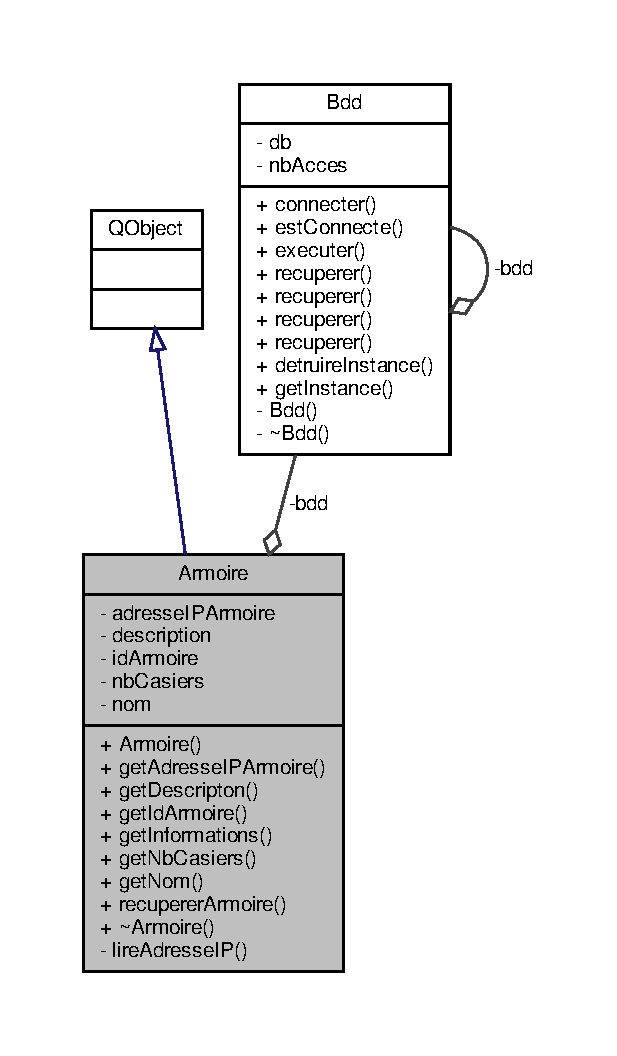
\includegraphics[width=296pt]{class_armoire__coll__graph}
\end{center}
\end{figure}
\subsubsection*{Signaux}
\begin{DoxyCompactItemize}
\item 
void \hyperlink{class_armoire_a1fc00ceaa842f579ee31c532a9b01508}{informations\+Armoire} (Q\+String\+List)
\end{DoxyCompactItemize}
\subsubsection*{Fonctions membres publiques}
\begin{DoxyCompactItemize}
\item 
\hyperlink{class_armoire_a5db260c682a9d2688afc0efbd5be8d14}{Armoire} (\hyperlink{class_q_object}{Q\+Object} $\ast$parent=nullptr)
\begin{DoxyCompactList}\small\item\em Définition du constructeur de la classe \hyperlink{class_armoire}{Armoire}. \end{DoxyCompactList}\item 
Q\+String \hyperlink{class_armoire_a706def736570580d7e5e3d2e29321c66}{get\+Adresse\+I\+P\+Armoire} () const
\begin{DoxyCompactList}\small\item\em Définition de la méthode get\+Adresse\+I\+P\+Armoire. \end{DoxyCompactList}\item 
Q\+String \hyperlink{class_armoire_a19af26aa7dedd03202d2484744dcad76}{get\+Descripton} () const
\begin{DoxyCompactList}\small\item\em Définition de la méthode get\+Descripton. \end{DoxyCompactList}\item 
Q\+String \hyperlink{class_armoire_a1a76e497170632b30f9821b396d53cec}{get\+Id\+Armoire} () const
\begin{DoxyCompactList}\small\item\em Définition de la méthode get\+Id\+Armoire. \end{DoxyCompactList}\item 
Q\+String\+List \hyperlink{class_armoire_a3e4d2ffc2fb91dd24d1160305ad36555}{get\+Informations} ()
\begin{DoxyCompactList}\small\item\em Définition de la méthode get\+Informations. \end{DoxyCompactList}\item 
Q\+String \hyperlink{class_armoire_aa94faaf53b6da5139a22a2ab21d4cf12}{get\+Nb\+Casiers} () const
\begin{DoxyCompactList}\small\item\em Définition de la méthode get\+Nb\+Casiers. \end{DoxyCompactList}\item 
Q\+String \hyperlink{class_armoire_a0045e45e0c9a465af765667344ce8bee}{get\+Nom} () const
\begin{DoxyCompactList}\small\item\em Définition de la méthode get\+Nom. \end{DoxyCompactList}\item 
void \hyperlink{class_armoire_a1c5266f9e4b01c0d2e1d244d2f11fffd}{recuperer\+Armoire} (Q\+String \hyperlink{class_armoire_a131caceb7d4b90cb7761851757e80f57}{id\+Armoire}=\char`\"{}1\char`\"{})
\begin{DoxyCompactList}\small\item\em Définition de la méthode recuperer\+Armoire. \end{DoxyCompactList}\item 
\hyperlink{class_armoire_a0f506a879391a987f12f59a23f60634e}{$\sim$\+Armoire} ()
\begin{DoxyCompactList}\small\item\em Définition du destructeur de la classe \hyperlink{class_armoire}{Armoire}. \end{DoxyCompactList}\end{DoxyCompactItemize}
\subsubsection*{Fonctions membres privées}
\begin{DoxyCompactItemize}
\item 
Q\+String \hyperlink{class_armoire_abc30649cc7d4f3c0cefcc54894aeb406}{lire\+Adresse\+IP} ()
\begin{DoxyCompactList}\small\item\em Définition de la méthode lire\+Adresse\+IP. \end{DoxyCompactList}\end{DoxyCompactItemize}
\subsubsection*{Attributs privés}
\begin{DoxyCompactItemize}
\item 
Q\+String \hyperlink{class_armoire_ab96bd042aa78eaefba0aefb860684ca6}{adresse\+I\+P\+Armoire}
\begin{DoxyCompactList}\small\item\em l\textquotesingle{}adresse IP de la Raspberry Pi \end{DoxyCompactList}\item 
\hyperlink{class_bdd}{Bdd} $\ast$ \hyperlink{class_armoire_a555f656018e7b600987128cdc792e320}{bdd}
\begin{DoxyCompactList}\small\item\em association d\textquotesingle{}un objet \hyperlink{class_bdd}{Bdd} (accès à la base de données) \end{DoxyCompactList}\item 
Q\+String \hyperlink{class_armoire_aa18be328693d7602439c779e30156c02}{description}
\begin{DoxyCompactList}\small\item\em la description de l\textquotesingle{}armoire \end{DoxyCompactList}\item 
Q\+String \hyperlink{class_armoire_a131caceb7d4b90cb7761851757e80f57}{id\+Armoire}
\begin{DoxyCompactList}\small\item\em l\textquotesingle{}id de l\textquotesingle{}armoire \end{DoxyCompactList}\item 
Q\+String \hyperlink{class_armoire_a9c4e926b7cddb13d097b75b3f5ef3de8}{nb\+Casiers}
\begin{DoxyCompactList}\small\item\em le nombre de casiers dans l\textquotesingle{}armoire \end{DoxyCompactList}\item 
Q\+String \hyperlink{class_armoire_a1de028da0fa3f085e2feaad8311d8795}{nom}
\begin{DoxyCompactList}\small\item\em le nom de l\textquotesingle{}armoire \end{DoxyCompactList}\end{DoxyCompactItemize}


\subsubsection{Description détaillée}
La classe \hyperlink{class_armoire}{Armoire} traite les articles. 

\begin{DoxyAuthor}{Auteur}
Tranchat Joffrey
\end{DoxyAuthor}
\begin{DoxyVersion}{Version}
1.\+0
\end{DoxyVersion}
\begin{DoxyDate}{Date}
Dimanche 22 Mars 2020 
\end{DoxyDate}


Définition à la ligne \hyperlink{_armoire_8h_source_l00049}{49} du fichier \hyperlink{_armoire_8h_source}{Armoire.\+h}.



\subsubsection{Documentation des constructeurs et destructeur}
\mbox{\Hypertarget{class_armoire_a5db260c682a9d2688afc0efbd5be8d14}\label{class_armoire_a5db260c682a9d2688afc0efbd5be8d14}} 
\index{Armoire@{Armoire}!Armoire@{Armoire}}
\index{Armoire@{Armoire}!Armoire@{Armoire}}
\paragraph{\texorpdfstring{Armoire()}{Armoire()}}
{\footnotesize\ttfamily Armoire\+::\+Armoire (\begin{DoxyParamCaption}\item[{\hyperlink{class_q_object}{Q\+Object} $\ast$}]{parent = {\ttfamily nullptr} }\end{DoxyParamCaption})}



Définition du constructeur de la classe \hyperlink{class_armoire}{Armoire}. 

Initialise un objet \hyperlink{class_armoire}{Armoire} 
\begin{DoxyParams}{Paramètres}
{\em parent} & l\textquotesingle{}objet \hyperlink{class_q_object}{Q\+Object} parent \\
\hline
\end{DoxyParams}


Définition à la ligne \hyperlink{_armoire_8cpp_source_l00022}{22} du fichier \hyperlink{_armoire_8cpp_source}{Armoire.\+cpp}.



Références \hyperlink{_armoire_8h_source_l00070}{adresse\+I\+P\+Armoire}, \hyperlink{_armoire_8h_source_l00065}{bdd}, \hyperlink{_bdd_8cpp_source_l00053}{Bdd\+::get\+Instance()}, \hyperlink{_armoire_8cpp_source_l00149}{lire\+Adresse\+I\+P()}, et \hyperlink{_armoire_8cpp_source_l00049}{recuperer\+Armoire()}.


\begin{DoxyCode}
00022                                 : \hyperlink{class_q_object}{QObject}(parent)
00023 \{
00024 \textcolor{preprocessor}{    #ifdef DEBUG\_ARMOIRE}
00025         qDebug() << Q\_FUNC\_INFO;
00026 \textcolor{preprocessor}{    #endif}
00027     \hyperlink{class_armoire_a555f656018e7b600987128cdc792e320}{bdd} = \hyperlink{class_bdd_a6f55c29d593da12ca31fad02f5adfe24}{Bdd::getInstance}();
00028     \hyperlink{class_armoire_ab96bd042aa78eaefba0aefb860684ca6}{adresseIPArmoire} = \hyperlink{class_armoire_abc30649cc7d4f3c0cefcc54894aeb406}{lireAdresseIP}();
00029     \hyperlink{class_armoire_a1c5266f9e4b01c0d2e1d244d2f11fffd}{recupererArmoire}();
00030 \}
\end{DoxyCode}
\mbox{\Hypertarget{class_armoire_a0f506a879391a987f12f59a23f60634e}\label{class_armoire_a0f506a879391a987f12f59a23f60634e}} 
\index{Armoire@{Armoire}!````~Armoire@{$\sim$\+Armoire}}
\index{````~Armoire@{$\sim$\+Armoire}!Armoire@{Armoire}}
\paragraph{\texorpdfstring{$\sim$\+Armoire()}{~Armoire()}}
{\footnotesize\ttfamily Armoire\+::$\sim$\+Armoire (\begin{DoxyParamCaption}{ }\end{DoxyParamCaption})}



Définition du destructeur de la classe \hyperlink{class_armoire}{Armoire}. 

Detruit un objet \hyperlink{class_armoire}{Armoire} 

Définition à la ligne \hyperlink{_armoire_8cpp_source_l00036}{36} du fichier \hyperlink{_armoire_8cpp_source}{Armoire.\+cpp}.



Références \hyperlink{_bdd_8cpp_source_l00073}{Bdd\+::detruire\+Instance()}.


\begin{DoxyCode}
00037 \{
00038     \hyperlink{class_bdd_af89fa3ffa107c7859a3964bf032cfdb7}{Bdd::detruireInstance}();
00039 \textcolor{preprocessor}{    #ifdef DEBUG\_ARMOIRE}
00040         qDebug() << Q\_FUNC\_INFO;
00041 \textcolor{preprocessor}{    #endif}
00042 \}
\end{DoxyCode}


\subsubsection{Documentation des fonctions membres}
\mbox{\Hypertarget{class_armoire_a706def736570580d7e5e3d2e29321c66}\label{class_armoire_a706def736570580d7e5e3d2e29321c66}} 
\index{Armoire@{Armoire}!get\+Adresse\+I\+P\+Armoire@{get\+Adresse\+I\+P\+Armoire}}
\index{get\+Adresse\+I\+P\+Armoire@{get\+Adresse\+I\+P\+Armoire}!Armoire@{Armoire}}
\paragraph{\texorpdfstring{get\+Adresse\+I\+P\+Armoire()}{getAdresseIPArmoire()}}
{\footnotesize\ttfamily Q\+String Armoire\+::get\+Adresse\+I\+P\+Armoire (\begin{DoxyParamCaption}{ }\end{DoxyParamCaption}) const}



Définition de la méthode get\+Adresse\+I\+P\+Armoire. 

renvoie l\textquotesingle{}adresse IP de l\textquotesingle{}armoire \begin{DoxyReturn}{Renvoie}
l\textquotesingle{}adresse IP de l\textquotesingle{}armoire 
\end{DoxyReturn}


Définition à la ligne \hyperlink{_armoire_8cpp_source_l00138}{138} du fichier \hyperlink{_armoire_8cpp_source}{Armoire.\+cpp}.



Références \hyperlink{_armoire_8h_source_l00070}{adresse\+I\+P\+Armoire}.


\begin{DoxyCode}
00139 \{
00140     \textcolor{keywordflow}{return} \hyperlink{class_armoire_ab96bd042aa78eaefba0aefb860684ca6}{adresseIPArmoire};
00141 \}
\end{DoxyCode}
\mbox{\Hypertarget{class_armoire_a19af26aa7dedd03202d2484744dcad76}\label{class_armoire_a19af26aa7dedd03202d2484744dcad76}} 
\index{Armoire@{Armoire}!get\+Descripton@{get\+Descripton}}
\index{get\+Descripton@{get\+Descripton}!Armoire@{Armoire}}
\paragraph{\texorpdfstring{get\+Descripton()}{getDescripton()}}
{\footnotesize\ttfamily Q\+String Armoire\+::get\+Descripton (\begin{DoxyParamCaption}{ }\end{DoxyParamCaption}) const}



Définition de la méthode get\+Descripton. 

renvoie la description de l\textquotesingle{}armoire \begin{DoxyReturn}{Renvoie}
la description de l\textquotesingle{}armoire 
\end{DoxyReturn}


Définition à la ligne \hyperlink{_armoire_8cpp_source_l00116}{116} du fichier \hyperlink{_armoire_8cpp_source}{Armoire.\+cpp}.



Références \hyperlink{_armoire_8h_source_l00068}{description}.


\begin{DoxyCode}
00117 \{
00118     \textcolor{keywordflow}{return} \hyperlink{class_armoire_aa18be328693d7602439c779e30156c02}{description};
00119 \}
\end{DoxyCode}
\mbox{\Hypertarget{class_armoire_a1a76e497170632b30f9821b396d53cec}\label{class_armoire_a1a76e497170632b30f9821b396d53cec}} 
\index{Armoire@{Armoire}!get\+Id\+Armoire@{get\+Id\+Armoire}}
\index{get\+Id\+Armoire@{get\+Id\+Armoire}!Armoire@{Armoire}}
\paragraph{\texorpdfstring{get\+Id\+Armoire()}{getIdArmoire()}}
{\footnotesize\ttfamily Q\+String Armoire\+::get\+Id\+Armoire (\begin{DoxyParamCaption}{ }\end{DoxyParamCaption}) const}



Définition de la méthode get\+Id\+Armoire. 

renvoie l\textquotesingle{}id de l\textquotesingle{}armoire \begin{DoxyReturn}{Renvoie}
id de l\textquotesingle{}armoire 
\end{DoxyReturn}


Définition à la ligne \hyperlink{_armoire_8cpp_source_l00094}{94} du fichier \hyperlink{_armoire_8cpp_source}{Armoire.\+cpp}.



Références \hyperlink{_armoire_8h_source_l00066}{id\+Armoire}.


\begin{DoxyCode}
00095 \{
00096     \textcolor{keywordflow}{return} \hyperlink{class_armoire_a131caceb7d4b90cb7761851757e80f57}{idArmoire};
00097 \}
\end{DoxyCode}
\mbox{\Hypertarget{class_armoire_a3e4d2ffc2fb91dd24d1160305ad36555}\label{class_armoire_a3e4d2ffc2fb91dd24d1160305ad36555}} 
\index{Armoire@{Armoire}!get\+Informations@{get\+Informations}}
\index{get\+Informations@{get\+Informations}!Armoire@{Armoire}}
\paragraph{\texorpdfstring{get\+Informations()}{getInformations()}}
{\footnotesize\ttfamily Q\+String\+List Armoire\+::get\+Informations (\begin{DoxyParamCaption}{ }\end{DoxyParamCaption})}



Définition de la méthode get\+Informations. 

renvoie les informations de l\textquotesingle{}armoire \begin{DoxyReturn}{Renvoie}
informations de l\textquotesingle{}armoire 
\end{DoxyReturn}


Définition à la ligne \hyperlink{_armoire_8cpp_source_l00078}{78} du fichier \hyperlink{_armoire_8cpp_source}{Armoire.\+cpp}.



Références \hyperlink{_armoire_8h_source_l00070}{adresse\+I\+P\+Armoire}, \hyperlink{_armoire_8h_source_l00068}{description}, \hyperlink{_armoire_8h_source_l00066}{id\+Armoire}, \hyperlink{class_armoire_a1fc00ceaa842f579ee31c532a9b01508}{informations\+Armoire()}, \hyperlink{_armoire_8h_source_l00069}{nb\+Casiers}, et \hyperlink{_armoire_8h_source_l00067}{nom}.



Référencé par \hyperlink{_supervision_8cpp_source_l00111}{Supervision\+::get\+Informations\+Armoire()}.


\begin{DoxyCode}
00079 \{
00080     QStringList informations;
00081 
00082     informations << \hyperlink{class_armoire_a131caceb7d4b90cb7761851757e80f57}{idArmoire} << \hyperlink{class_armoire_a1de028da0fa3f085e2feaad8311d8795}{nom} << \hyperlink{class_armoire_aa18be328693d7602439c779e30156c02}{description} << 
      \hyperlink{class_armoire_a9c4e926b7cddb13d097b75b3f5ef3de8}{nbCasiers} << \hyperlink{class_armoire_ab96bd042aa78eaefba0aefb860684ca6}{adresseIPArmoire};
00083 
00084     emit \hyperlink{class_armoire_a1fc00ceaa842f579ee31c532a9b01508}{informationsArmoire}(informations);
00085 
00086     \textcolor{keywordflow}{return} informations;
00087 \}
\end{DoxyCode}
\mbox{\Hypertarget{class_armoire_aa94faaf53b6da5139a22a2ab21d4cf12}\label{class_armoire_aa94faaf53b6da5139a22a2ab21d4cf12}} 
\index{Armoire@{Armoire}!get\+Nb\+Casiers@{get\+Nb\+Casiers}}
\index{get\+Nb\+Casiers@{get\+Nb\+Casiers}!Armoire@{Armoire}}
\paragraph{\texorpdfstring{get\+Nb\+Casiers()}{getNbCasiers()}}
{\footnotesize\ttfamily Q\+String Armoire\+::get\+Nb\+Casiers (\begin{DoxyParamCaption}{ }\end{DoxyParamCaption}) const}



Définition de la méthode get\+Nb\+Casiers. 

renvoie le nombre de casiers dans l\textquotesingle{}armoire \begin{DoxyReturn}{Renvoie}
le nombre de casiers dans l\textquotesingle{}armoire 
\end{DoxyReturn}


Définition à la ligne \hyperlink{_armoire_8cpp_source_l00127}{127} du fichier \hyperlink{_armoire_8cpp_source}{Armoire.\+cpp}.



Références \hyperlink{_armoire_8h_source_l00069}{nb\+Casiers}.



Référencé par \hyperlink{_supervision_8cpp_source_l00090}{Supervision\+::creer\+Casiers()}.


\begin{DoxyCode}
00128 \{
00129     \textcolor{keywordflow}{return} \hyperlink{class_armoire_a9c4e926b7cddb13d097b75b3f5ef3de8}{nbCasiers};
00130 \}
\end{DoxyCode}
\mbox{\Hypertarget{class_armoire_a0045e45e0c9a465af765667344ce8bee}\label{class_armoire_a0045e45e0c9a465af765667344ce8bee}} 
\index{Armoire@{Armoire}!get\+Nom@{get\+Nom}}
\index{get\+Nom@{get\+Nom}!Armoire@{Armoire}}
\paragraph{\texorpdfstring{get\+Nom()}{getNom()}}
{\footnotesize\ttfamily Q\+String Armoire\+::get\+Nom (\begin{DoxyParamCaption}{ }\end{DoxyParamCaption}) const}



Définition de la méthode get\+Nom. 

renvoie le nom de l\textquotesingle{}armoire \begin{DoxyReturn}{Renvoie}
le nom de l\textquotesingle{}armoire 
\end{DoxyReturn}


Définition à la ligne \hyperlink{_armoire_8cpp_source_l00105}{105} du fichier \hyperlink{_armoire_8cpp_source}{Armoire.\+cpp}.



Références \hyperlink{_armoire_8h_source_l00067}{nom}.


\begin{DoxyCode}
00106 \{
00107     \textcolor{keywordflow}{return} \hyperlink{class_armoire_a1de028da0fa3f085e2feaad8311d8795}{nom};
00108 \}
\end{DoxyCode}
\mbox{\Hypertarget{class_armoire_a1fc00ceaa842f579ee31c532a9b01508}\label{class_armoire_a1fc00ceaa842f579ee31c532a9b01508}} 
\index{Armoire@{Armoire}!informations\+Armoire@{informations\+Armoire}}
\index{informations\+Armoire@{informations\+Armoire}!Armoire@{Armoire}}
\paragraph{\texorpdfstring{informations\+Armoire}{informationsArmoire}}
{\footnotesize\ttfamily void Armoire\+::informations\+Armoire (\begin{DoxyParamCaption}\item[{Q\+String\+List}]{ }\end{DoxyParamCaption})\hspace{0.3cm}{\ttfamily [signal]}}



Référencé par \hyperlink{_armoire_8cpp_source_l00078}{get\+Informations()}.

\mbox{\Hypertarget{class_armoire_abc30649cc7d4f3c0cefcc54894aeb406}\label{class_armoire_abc30649cc7d4f3c0cefcc54894aeb406}} 
\index{Armoire@{Armoire}!lire\+Adresse\+IP@{lire\+Adresse\+IP}}
\index{lire\+Adresse\+IP@{lire\+Adresse\+IP}!Armoire@{Armoire}}
\paragraph{\texorpdfstring{lire\+Adresse\+I\+P()}{lireAdresseIP()}}
{\footnotesize\ttfamily Q\+String Armoire\+::lire\+Adresse\+IP (\begin{DoxyParamCaption}{ }\end{DoxyParamCaption})\hspace{0.3cm}{\ttfamily [private]}}



Définition de la méthode lire\+Adresse\+IP. 

Récupère l\textquotesingle{}adresse IP de la Raspberry Pi \begin{DoxyReturn}{Renvoie}
l\textquotesingle{}adresse IP de la Raspberry Pi 
\end{DoxyReturn}


Définition à la ligne \hyperlink{_armoire_8cpp_source_l00149}{149} du fichier \hyperlink{_armoire_8cpp_source}{Armoire.\+cpp}.



Référencé par \hyperlink{_armoire_8cpp_source_l00022}{Armoire()}.


\begin{DoxyCode}
00150 \{
00151     QStringList adresses;
00152     \textcolor{keywordflow}{foreach}(QHostAddress adresse, QNetworkInterface::allAddresses())
00153     \{
00154         \textcolor{comment}{// Filtre les adresses localhost ...}
00155         \textcolor{keywordflow}{if}(adresse != QHostAddress::LocalHostIPv6
00156            && adresse != QHostAddress::LocalHost
00157            \textcolor{comment}{// ... APIPA ...}
00158            && !adresse.isInSubnet(QHostAddress::parseSubnet(\textcolor{stringliteral}{"169.254.0.0/16"}))
00159            \textcolor{comment}{// ... Lien Local IPv6}
00160            && !adresse.isInSubnet(QHostAddress::parseSubnet(\textcolor{stringliteral}{"FE80::/64"})))
00161         \{
00162             qDebug() << Q\_FUNC\_INFO << adresse.toString();
00163             adresses << adresse.toString();
00164         \}
00165     \}
00166 
00167     \textcolor{keywordflow}{foreach}(QString adresse, adresses)
00168     \{
00169 \textcolor{preprocessor}{        #ifdef DEBUG\_ARMOIRE}
00170             qDebug() << Q\_FUNC\_INFO << adresse;
00171 \textcolor{preprocessor}{        #endif}
00172         \textcolor{keywordflow}{if}(adresse.contains(\textcolor{stringliteral}{"192."}))
00173             \textcolor{keywordflow}{return} adresse;
00174     \}
00175 
00176     \textcolor{comment}{/*if(adresses.count() > 0)}
00177 \textcolor{comment}{    \{}
00178 \textcolor{comment}{        return adresses.at(0);}
00179 \textcolor{comment}{    \}*/}
00180 
00181     \textcolor{keywordflow}{return} QString(\textcolor{stringliteral}{""});
00182 \}
\end{DoxyCode}
\mbox{\Hypertarget{class_armoire_a1c5266f9e4b01c0d2e1d244d2f11fffd}\label{class_armoire_a1c5266f9e4b01c0d2e1d244d2f11fffd}} 
\index{Armoire@{Armoire}!recuperer\+Armoire@{recuperer\+Armoire}}
\index{recuperer\+Armoire@{recuperer\+Armoire}!Armoire@{Armoire}}
\paragraph{\texorpdfstring{recuperer\+Armoire()}{recupererArmoire()}}
{\footnotesize\ttfamily void Armoire\+::recuperer\+Armoire (\begin{DoxyParamCaption}\item[{Q\+String}]{id\+Armoire = {\ttfamily \char`\"{}1\char`\"{}} }\end{DoxyParamCaption})}



Définition de la méthode recuperer\+Armoire. 

Récupère les données de l\textquotesingle{}armoire dans la base de données 
\begin{DoxyParams}{Paramètres}
{\em id\+Armoire} & l\textquotesingle{}id de l\textquotesingle{}armoire \\
\hline
\end{DoxyParams}


Définition à la ligne \hyperlink{_armoire_8cpp_source_l00049}{49} du fichier \hyperlink{_armoire_8cpp_source}{Armoire.\+cpp}.



Références \hyperlink{_armoire_8h_source_l00065}{bdd}, \hyperlink{_armoire_8h_source_l00068}{description}, \hyperlink{_armoire_8h_source_l00069}{nb\+Casiers}, \hyperlink{_armoire_8h_source_l00067}{nom}, \hyperlink{_bdd_8cpp_source_l00187}{Bdd\+::recuperer()}, \hyperlink{_armoire_8h_source_l00031}{T\+A\+B\+L\+E\+\_\+\+A\+R\+M\+O\+I\+R\+E\+\_\+\+D\+E\+S\+C\+R\+I\+P\+T\+I\+ON}, \hyperlink{_armoire_8h_source_l00029}{T\+A\+B\+L\+E\+\_\+\+A\+R\+M\+O\+I\+R\+E\+\_\+\+I\+D\+\_\+\+A\+R\+M\+O\+I\+RE}, \hyperlink{_armoire_8h_source_l00032}{T\+A\+B\+L\+E\+\_\+\+A\+R\+M\+O\+I\+R\+E\+\_\+\+N\+B\+\_\+\+C\+A\+S\+I\+E\+RS}, et \hyperlink{_armoire_8h_source_l00030}{T\+A\+B\+L\+E\+\_\+\+A\+R\+M\+O\+I\+R\+E\+\_\+\+N\+OM}.



Référencé par \hyperlink{_armoire_8cpp_source_l00022}{Armoire()}.


\begin{DoxyCode}
00050 \{
00051     QString requeteBDD;
00052 
00053     \textcolor{keywordflow}{if}(!\hyperlink{class_armoire_a131caceb7d4b90cb7761851757e80f57}{idArmoire}.isEmpty()) \textcolor{comment}{// par id}
00054     \{
00055         requeteBDD = \textcolor{stringliteral}{"SELECT * from Armoire where idArmoire = '"} + \hyperlink{class_armoire_a131caceb7d4b90cb7761851757e80f57}{idArmoire} + \textcolor{stringliteral}{"'"};
00056         QStringList donnees;
00057         \hyperlink{class_armoire_a555f656018e7b600987128cdc792e320}{bdd}->\hyperlink{class_bdd_a8f25d29d309041bbf875700db0efd97b}{recuperer}(requeteBDD, donnees);
00058 
00059 \textcolor{preprocessor}{        #ifdef DEBUG\_ARMOIRE}
00060             qDebug() << Q\_FUNC\_INFO << donnees;
00061 \textcolor{preprocessor}{        #endif}
00062 
00063         \textcolor{keywordflow}{if}(donnees.size() > 0)
00064         \{
00065             this->\hyperlink{class_armoire_a131caceb7d4b90cb7761851757e80f57}{idArmoire} = donnees.at(\hyperlink{_armoire_8h_a8c8e83929e4df868beea17eda4fb5dada167bbea3f9d799583c77d0a6b12ed99e}{TABLE\_ARMOIRE\_ID\_ARMOIRE});
00066             \hyperlink{class_armoire_a1de028da0fa3f085e2feaad8311d8795}{nom} = donnees.at(\hyperlink{_armoire_8h_a8c8e83929e4df868beea17eda4fb5dadaed87f53039b2f5f5401a4b4c9ea8a706}{TABLE\_ARMOIRE\_NOM});
00067             \hyperlink{class_armoire_aa18be328693d7602439c779e30156c02}{description} = donnees.at(\hyperlink{_armoire_8h_a8c8e83929e4df868beea17eda4fb5dadaa46613f3c7eb048c8392fb780e801cc8}{TABLE\_ARMOIRE\_DESCRIPTION});
00068             \hyperlink{class_armoire_a9c4e926b7cddb13d097b75b3f5ef3de8}{nbCasiers} = donnees.at(\hyperlink{_armoire_8h_a8c8e83929e4df868beea17eda4fb5dada92634af3316ad54be209ef14cc8a8981}{TABLE\_ARMOIRE\_NB\_CASIERS});
00069         \}
00070     \}    
00071 \}
\end{DoxyCode}


\subsubsection{Documentation des données membres}
\mbox{\Hypertarget{class_armoire_ab96bd042aa78eaefba0aefb860684ca6}\label{class_armoire_ab96bd042aa78eaefba0aefb860684ca6}} 
\index{Armoire@{Armoire}!adresse\+I\+P\+Armoire@{adresse\+I\+P\+Armoire}}
\index{adresse\+I\+P\+Armoire@{adresse\+I\+P\+Armoire}!Armoire@{Armoire}}
\paragraph{\texorpdfstring{adresse\+I\+P\+Armoire}{adresseIPArmoire}}
{\footnotesize\ttfamily Q\+String Armoire\+::adresse\+I\+P\+Armoire\hspace{0.3cm}{\ttfamily [private]}}



l\textquotesingle{}adresse IP de la Raspberry Pi 



Définition à la ligne \hyperlink{_armoire_8h_source_l00070}{70} du fichier \hyperlink{_armoire_8h_source}{Armoire.\+h}.



Référencé par \hyperlink{_armoire_8cpp_source_l00022}{Armoire()}, \hyperlink{_armoire_8cpp_source_l00138}{get\+Adresse\+I\+P\+Armoire()}, et \hyperlink{_armoire_8cpp_source_l00078}{get\+Informations()}.

\mbox{\Hypertarget{class_armoire_a555f656018e7b600987128cdc792e320}\label{class_armoire_a555f656018e7b600987128cdc792e320}} 
\index{Armoire@{Armoire}!bdd@{bdd}}
\index{bdd@{bdd}!Armoire@{Armoire}}
\paragraph{\texorpdfstring{bdd}{bdd}}
{\footnotesize\ttfamily \hyperlink{class_bdd}{Bdd}$\ast$ Armoire\+::bdd\hspace{0.3cm}{\ttfamily [private]}}



association d\textquotesingle{}un objet \hyperlink{class_bdd}{Bdd} (accès à la base de données) 



Définition à la ligne \hyperlink{_armoire_8h_source_l00065}{65} du fichier \hyperlink{_armoire_8h_source}{Armoire.\+h}.



Référencé par \hyperlink{_armoire_8cpp_source_l00022}{Armoire()}, et \hyperlink{_armoire_8cpp_source_l00049}{recuperer\+Armoire()}.

\mbox{\Hypertarget{class_armoire_aa18be328693d7602439c779e30156c02}\label{class_armoire_aa18be328693d7602439c779e30156c02}} 
\index{Armoire@{Armoire}!description@{description}}
\index{description@{description}!Armoire@{Armoire}}
\paragraph{\texorpdfstring{description}{description}}
{\footnotesize\ttfamily Q\+String Armoire\+::description\hspace{0.3cm}{\ttfamily [private]}}



la description de l\textquotesingle{}armoire 



Définition à la ligne \hyperlink{_armoire_8h_source_l00068}{68} du fichier \hyperlink{_armoire_8h_source}{Armoire.\+h}.



Référencé par \hyperlink{_armoire_8cpp_source_l00116}{get\+Descripton()}, \hyperlink{_armoire_8cpp_source_l00078}{get\+Informations()}, et \hyperlink{_armoire_8cpp_source_l00049}{recuperer\+Armoire()}.

\mbox{\Hypertarget{class_armoire_a131caceb7d4b90cb7761851757e80f57}\label{class_armoire_a131caceb7d4b90cb7761851757e80f57}} 
\index{Armoire@{Armoire}!id\+Armoire@{id\+Armoire}}
\index{id\+Armoire@{id\+Armoire}!Armoire@{Armoire}}
\paragraph{\texorpdfstring{id\+Armoire}{idArmoire}}
{\footnotesize\ttfamily Q\+String Armoire\+::id\+Armoire\hspace{0.3cm}{\ttfamily [private]}}



l\textquotesingle{}id de l\textquotesingle{}armoire 



Définition à la ligne \hyperlink{_armoire_8h_source_l00066}{66} du fichier \hyperlink{_armoire_8h_source}{Armoire.\+h}.



Référencé par \hyperlink{_armoire_8cpp_source_l00094}{get\+Id\+Armoire()}, et \hyperlink{_armoire_8cpp_source_l00078}{get\+Informations()}.

\mbox{\Hypertarget{class_armoire_a9c4e926b7cddb13d097b75b3f5ef3de8}\label{class_armoire_a9c4e926b7cddb13d097b75b3f5ef3de8}} 
\index{Armoire@{Armoire}!nb\+Casiers@{nb\+Casiers}}
\index{nb\+Casiers@{nb\+Casiers}!Armoire@{Armoire}}
\paragraph{\texorpdfstring{nb\+Casiers}{nbCasiers}}
{\footnotesize\ttfamily Q\+String Armoire\+::nb\+Casiers\hspace{0.3cm}{\ttfamily [private]}}



le nombre de casiers dans l\textquotesingle{}armoire 



Définition à la ligne \hyperlink{_armoire_8h_source_l00069}{69} du fichier \hyperlink{_armoire_8h_source}{Armoire.\+h}.



Référencé par \hyperlink{_armoire_8cpp_source_l00078}{get\+Informations()}, \hyperlink{_armoire_8cpp_source_l00127}{get\+Nb\+Casiers()}, et \hyperlink{_armoire_8cpp_source_l00049}{recuperer\+Armoire()}.

\mbox{\Hypertarget{class_armoire_a1de028da0fa3f085e2feaad8311d8795}\label{class_armoire_a1de028da0fa3f085e2feaad8311d8795}} 
\index{Armoire@{Armoire}!nom@{nom}}
\index{nom@{nom}!Armoire@{Armoire}}
\paragraph{\texorpdfstring{nom}{nom}}
{\footnotesize\ttfamily Q\+String Armoire\+::nom\hspace{0.3cm}{\ttfamily [private]}}



le nom de l\textquotesingle{}armoire 



Définition à la ligne \hyperlink{_armoire_8h_source_l00067}{67} du fichier \hyperlink{_armoire_8h_source}{Armoire.\+h}.



Référencé par \hyperlink{_armoire_8cpp_source_l00078}{get\+Informations()}, \hyperlink{_armoire_8cpp_source_l00105}{get\+Nom()}, et \hyperlink{_armoire_8cpp_source_l00049}{recuperer\+Armoire()}.



La documentation de cette classe a été générée à partir des fichiers suivants \+:\begin{DoxyCompactItemize}
\item 
\hyperlink{_armoire_8h}{Armoire.\+h}\item 
\hyperlink{_armoire_8cpp}{Armoire.\+cpp}\end{DoxyCompactItemize}

\hypertarget{class_article}{}\subsection{Référence de la classe Article}
\label{class_article}\index{Article@{Article}}


La classe \hyperlink{class_article}{Article} traite les articles.  




{\ttfamily \#include $<$Article.\+h$>$}



Graphe de collaboration de Article\+:
\nopagebreak
\begin{figure}[H]
\begin{center}
\leavevmode
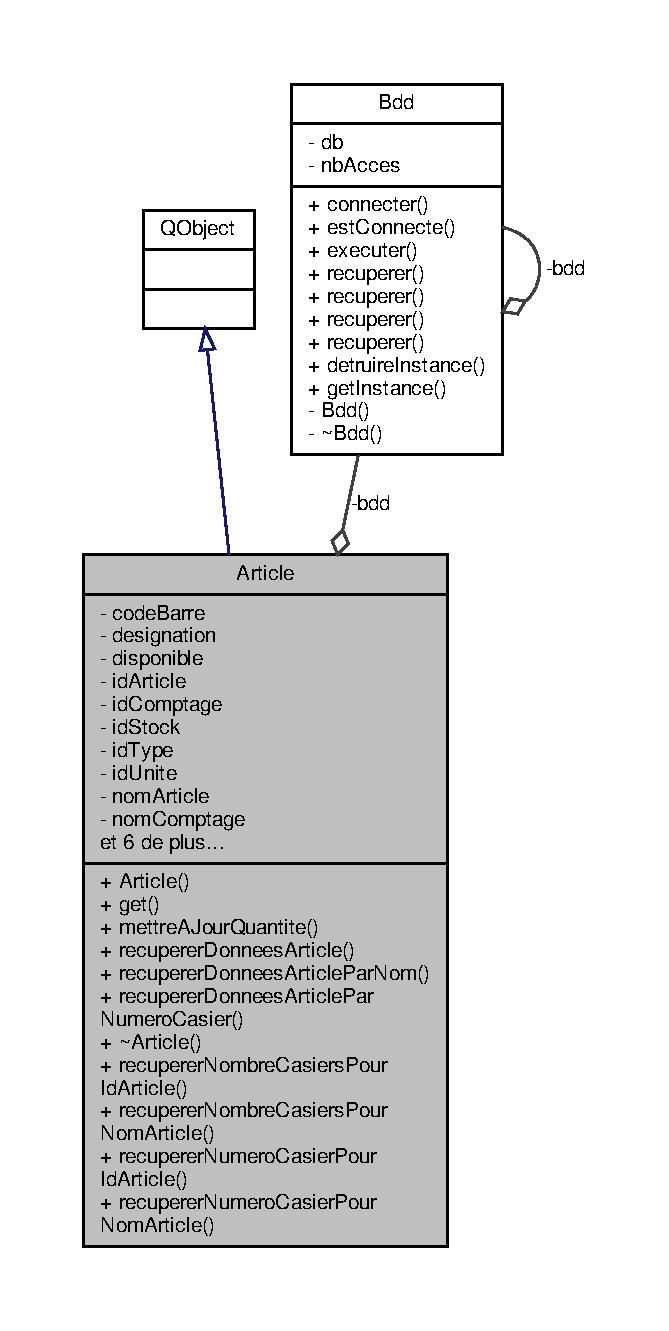
\includegraphics[height=550pt]{class_article__coll__graph}
\end{center}
\end{figure}
\subsubsection*{Fonctions membres publiques}
\begin{DoxyCompactItemize}
\item 
\hyperlink{class_article_a27b5b7af25138f7a465215be3a9deca4}{Article} (\hyperlink{class_q_object}{Q\+Object} $\ast$parent=nullptr)
\begin{DoxyCompactList}\small\item\em Définition du constructeur de la classe \hyperlink{class_article}{Article}. \end{DoxyCompactList}\item 
Q\+String \hyperlink{class_article_a81e89d4821991a69277f3a0f8e88a001}{get} (\hyperlink{_article_8h_a159354683cfd6e1b578172fbe6490ab6}{Champ\+Article} champ)
\begin{DoxyCompactList}\small\item\em Définition de la méthode get. \end{DoxyCompactList}\item 
void \hyperlink{class_article_a5777f36d74974ff21e712a9875c2d8bf}{mettre\+A\+Jour\+Quantite} (Q\+String \hyperlink{class_article_a0870104453080b43bc271346217a864b}{quantite})
\begin{DoxyCompactList}\small\item\em Définition de la méthode mettre\+A\+Jour\+Quantite. \end{DoxyCompactList}\item 
bool \hyperlink{class_article_ae657464da12790b763659ca98a948f50}{recuperer\+Donnees\+Article} (Q\+String \hyperlink{class_article_a9f2f7a04139f26accec145066a5aacae}{id\+Article}, int num\+Casier=0)
\begin{DoxyCompactList}\small\item\em Récupère les données d\textquotesingle{}un article de l\textquotesingle{}armoire dans la base de données par son id\+Article. \end{DoxyCompactList}\item 
bool \hyperlink{class_article_a6eab145b46f5e1786c5ddf669ffabb6e}{recuperer\+Donnees\+Article\+Par\+Nom} (Q\+String \hyperlink{class_article_a0ba6c08f7dd54e4b7caf673ecd6b41a6}{nom\+Article}, int num\+Casier=0)
\begin{DoxyCompactList}\small\item\em Récupère les données d\textquotesingle{}un article de l\textquotesingle{}armoire dans la base de données par son nom\+Article. \end{DoxyCompactList}\item 
bool \hyperlink{class_article_a5d8241c703f142bbc8b011f867fd953f}{recuperer\+Donnees\+Article\+Par\+Numero\+Casier} (Q\+String \hyperlink{class_article_a4b8dd9598cc16200c60c7f55196fc26d}{numero\+Casier})
\begin{DoxyCompactList}\small\item\em Définition de la méthode recuperer\+Donnees\+Article\+Par\+Numero\+Casier. \end{DoxyCompactList}\item 
\hyperlink{class_article_a5c429e49b30104b1069044d0e1a6aa1a}{$\sim$\+Article} ()
\begin{DoxyCompactList}\small\item\em Définition de la méthode $\sim$\+Article. \end{DoxyCompactList}\end{DoxyCompactItemize}
\subsubsection*{Fonctions membres publiques statiques}
\begin{DoxyCompactItemize}
\item 
static unsigned int \hyperlink{class_article_a537f0aa471a7466425b6abf6c34058d6}{recuperer\+Nombre\+Casiers\+Pour\+Id\+Article} (Q\+String \hyperlink{class_article_a9f2f7a04139f26accec145066a5aacae}{id\+Article})
\begin{DoxyCompactList}\small\item\em Définition de la méthode recuperer\+Nombre\+Casiers\+Pour\+Id\+Article. \end{DoxyCompactList}\item 
static unsigned int \hyperlink{class_article_acdd796ad55a7fde0c229c8c2df7050cc}{recuperer\+Nombre\+Casiers\+Pour\+Nom\+Article} (Q\+String \hyperlink{class_article_a0ba6c08f7dd54e4b7caf673ecd6b41a6}{nom\+Article})
\begin{DoxyCompactList}\small\item\em Définition de la méthode recuperer\+Nombre\+Casiers\+Pour\+Nom\+Article. \end{DoxyCompactList}\item 
static Q\+Vector$<$ Q\+String $>$ \hyperlink{class_article_aa7aeaee7858b50714e9c022899b9b82d}{recuperer\+Numero\+Casier\+Pour\+Id\+Article} (Q\+String \hyperlink{class_article_a9f2f7a04139f26accec145066a5aacae}{id\+Article})
\begin{DoxyCompactList}\small\item\em Définition de la méthode recuperer\+Numero\+Casier\+Pour\+Id\+Article. \end{DoxyCompactList}\item 
static Q\+Vector$<$ Q\+String $>$ \hyperlink{class_article_aa311f3d149340622383c418444aa65a4}{recuperer\+Numero\+Casier\+Pour\+Nom\+Article} (Q\+String \hyperlink{class_article_a0ba6c08f7dd54e4b7caf673ecd6b41a6}{nom\+Article})
\begin{DoxyCompactList}\small\item\em Définition de la méthode recuperer\+Numero\+Casier\+Pour\+Nom\+Article. \end{DoxyCompactList}\end{DoxyCompactItemize}
\subsubsection*{Attributs privés}
\begin{DoxyCompactItemize}
\item 
Q\+String \hyperlink{class_article_a28db45ee4a48155c297be5c7c2eb54b9}{code\+Barre}
\begin{DoxyCompactList}\small\item\em code\+Barre de l\textquotesingle{}article récupéré \end{DoxyCompactList}\item 
Q\+String \hyperlink{class_article_a46a953cc2b35c8d868b27e8fa21c7a3a}{designation}
\begin{DoxyCompactList}\small\item\em designation de l\textquotesingle{}article récupéré \end{DoxyCompactList}\item 
Q\+String \hyperlink{class_article_ac361aa1f57e32243854735e84c6891e2}{disponible}
\begin{DoxyCompactList}\small\item\em disponibilité de l\textquotesingle{}article récupéré \end{DoxyCompactList}\item 
Q\+String \hyperlink{class_article_a9f2f7a04139f26accec145066a5aacae}{id\+Article}
\begin{DoxyCompactList}\small\item\em id\+Article de l\textquotesingle{}article récupéré \end{DoxyCompactList}\item 
Q\+String \hyperlink{class_article_adc8cef4c963c0fcc6d486dab4bd60e17}{id\+Comptage}
\begin{DoxyCompactList}\small\item\em id\+Comptage de l\textquotesingle{}article récupéré \end{DoxyCompactList}\item 
Q\+String \hyperlink{class_article_afb7785930598d5fbdafb707acdd3eec1}{id\+Stock}
\begin{DoxyCompactList}\small\item\em id\+Stock de l\textquotesingle{}article récupéré \end{DoxyCompactList}\item 
Q\+String \hyperlink{class_article_a1586203d0eb334a3298ca719f924083d}{id\+Type}
\begin{DoxyCompactList}\small\item\em id\+Type de l\textquotesingle{}article récupéré \end{DoxyCompactList}\item 
Q\+String \hyperlink{class_article_a702cff16cb9cd0774383ceba81d83869}{id\+Unite}
\begin{DoxyCompactList}\small\item\em id\+Unite de l\textquotesingle{}article récupéré \end{DoxyCompactList}\item 
Q\+String \hyperlink{class_article_a0ba6c08f7dd54e4b7caf673ecd6b41a6}{nom\+Article}
\begin{DoxyCompactList}\small\item\em nom\+Article de l\textquotesingle{}article récupéré \end{DoxyCompactList}\item 
Q\+String \hyperlink{class_article_a1953a03d4505797952054141dbb2e327}{nom\+Comptage}
\begin{DoxyCompactList}\small\item\em nom\+Comptage de l\textquotesingle{}article récupéré \end{DoxyCompactList}\item 
Q\+String \hyperlink{class_article_a06489a7445495277e44c7179b7cf8bbc}{nom\+Type}
\begin{DoxyCompactList}\small\item\em nom\+Type de l\textquotesingle{}article récupéré \end{DoxyCompactList}\item 
Q\+String \hyperlink{class_article_a43a20e248e57150af0546c9f4b6b74c3}{nom\+Unite}
\begin{DoxyCompactList}\small\item\em nom\+Unite de l\textquotesingle{}article récupéré \end{DoxyCompactList}\item 
Q\+String \hyperlink{class_article_a4b8dd9598cc16200c60c7f55196fc26d}{numero\+Casier}
\begin{DoxyCompactList}\small\item\em numero\+Casier de l\textquotesingle{}article récupéré \end{DoxyCompactList}\item 
Q\+String \hyperlink{class_article_ac42217ed32ef1466b099f3e4a6a913f0}{poids\+Article}
\begin{DoxyCompactList}\small\item\em poids\+Article de l\textquotesingle{}article récupéré \end{DoxyCompactList}\item 
Q\+String \hyperlink{class_article_a0870104453080b43bc271346217a864b}{quantite}
\begin{DoxyCompactList}\small\item\em quantite de l\textquotesingle{}article récupéré \end{DoxyCompactList}\item 
Q\+String \hyperlink{class_article_abacf2d29d4b2e3e7b49256bc48d5fe64}{tare}
\begin{DoxyCompactList}\small\item\em tare du numéro de casier de l\textquotesingle{}article récupéré \end{DoxyCompactList}\end{DoxyCompactItemize}
\subsubsection*{Attributs privés statiques}
\begin{DoxyCompactItemize}
\item 
static \hyperlink{class_bdd}{Bdd} $\ast$ \hyperlink{class_article_a7221cec4212d86d74f479b9ee683ee8a}{bdd} = \hyperlink{class_bdd_a6f55c29d593da12ca31fad02f5adfe24}{Bdd\+::get\+Instance}()
\begin{DoxyCompactList}\small\item\em association d\textquotesingle{}un objet \hyperlink{class_bdd}{Bdd} (accès à la base de données) \end{DoxyCompactList}\end{DoxyCompactItemize}


\subsubsection{Description détaillée}
La classe \hyperlink{class_article}{Article} traite les articles. 

\begin{DoxyAuthor}{Auteur}
Tranchat Joffrey
\end{DoxyAuthor}
\begin{DoxyVersion}{Version}
1.\+0
\end{DoxyVersion}
\begin{DoxyDate}{Date}
Mercredi 11 Mars 2020 
\end{DoxyDate}


Définition à la ligne \hyperlink{_article_8h_source_l00063}{63} du fichier \hyperlink{_article_8h_source}{Article.\+h}.



\subsubsection{Documentation des constructeurs et destructeur}
\mbox{\Hypertarget{class_article_a27b5b7af25138f7a465215be3a9deca4}\label{class_article_a27b5b7af25138f7a465215be3a9deca4}} 
\index{Article@{Article}!Article@{Article}}
\index{Article@{Article}!Article@{Article}}
\paragraph{\texorpdfstring{Article()}{Article()}}
{\footnotesize\ttfamily Article\+::\+Article (\begin{DoxyParamCaption}\item[{\hyperlink{class_q_object}{Q\+Object} $\ast$}]{parent = {\ttfamily nullptr} }\end{DoxyParamCaption})}



Définition du constructeur de la classe \hyperlink{class_article}{Article}. 

Initialise un objet \hyperlink{class_article}{Article} 
\begin{DoxyParams}{Paramètres}
{\em parent} & l\textquotesingle{}objet \hyperlink{class_q_object}{Q\+Object} parent \\
\hline
\end{DoxyParams}


Définition à la ligne \hyperlink{_article_8cpp_source_l00024}{24} du fichier \hyperlink{_article_8cpp_source}{Article.\+cpp}.


\begin{DoxyCode}
00024                                 : \hyperlink{class_q_object}{QObject}(parent)
00025 \{
00026 \textcolor{preprocessor}{    #ifdef DEBUG\_ARTICLE}
00027         qDebug() << Q\_FUNC\_INFO;
00028 \textcolor{preprocessor}{    #endif}
00029     \textcolor{comment}{//bdd = Bdd::getInstance();}
00030 \}
\end{DoxyCode}
\mbox{\Hypertarget{class_article_a5c429e49b30104b1069044d0e1a6aa1a}\label{class_article_a5c429e49b30104b1069044d0e1a6aa1a}} 
\index{Article@{Article}!````~Article@{$\sim$\+Article}}
\index{````~Article@{$\sim$\+Article}!Article@{Article}}
\paragraph{\texorpdfstring{$\sim$\+Article()}{~Article()}}
{\footnotesize\ttfamily Article\+::$\sim$\+Article (\begin{DoxyParamCaption}{ }\end{DoxyParamCaption})}



Définition de la méthode $\sim$\+Article. 

Détruit un objet \hyperlink{class_article}{Article} 

Définition à la ligne \hyperlink{_article_8cpp_source_l00036}{36} du fichier \hyperlink{_article_8cpp_source}{Article.\+cpp}.


\begin{DoxyCode}
00037 \{
00038     \textcolor{comment}{//Bdd::detruireInstance();}
00039 \textcolor{preprocessor}{    #ifdef DEBUG\_ARTICLE}
00040         qDebug() << Q\_FUNC\_INFO;
00041 \textcolor{preprocessor}{    #endif}
00042 \}
\end{DoxyCode}


\subsubsection{Documentation des fonctions membres}
\mbox{\Hypertarget{class_article_a81e89d4821991a69277f3a0f8e88a001}\label{class_article_a81e89d4821991a69277f3a0f8e88a001}} 
\index{Article@{Article}!get@{get}}
\index{get@{get}!Article@{Article}}
\paragraph{\texorpdfstring{get()}{get()}}
{\footnotesize\ttfamily Q\+String Article\+::get (\begin{DoxyParamCaption}\item[{\hyperlink{_article_8h_a159354683cfd6e1b578172fbe6490ab6}{Champ\+Article}}]{champ }\end{DoxyParamCaption})}



Définition de la méthode get. 

Accesseur get pour les différents champs d\textquotesingle{}un \hyperlink{class_article}{Article} 
\begin{DoxyParams}{Paramètres}
{\em champ} & un champ de la table = un attribut \\
\hline
\end{DoxyParams}
\begin{DoxyReturn}{Renvoie}

\end{DoxyReturn}


Définition à la ligne \hyperlink{_article_8cpp_source_l00266}{266} du fichier \hyperlink{_article_8cpp_source}{Article.\+cpp}.



Références \hyperlink{_article_8h_source_l00090}{code\+Barre}, \hyperlink{_article_8h_source_l00091}{designation}, \hyperlink{_article_8h_source_l00093}{disponible}, \hyperlink{_article_8h_source_l00084}{id\+Article}, \hyperlink{_article_8h_source_l00088}{id\+Comptage}, \hyperlink{_article_8h_source_l00083}{id\+Stock}, \hyperlink{_article_8h_source_l00086}{id\+Type}, \hyperlink{_article_8h_source_l00096}{id\+Unite}, \hyperlink{_article_8h_source_l00085}{nom\+Article}, \hyperlink{_article_8h_source_l00089}{nom\+Comptage}, \hyperlink{_article_8h_source_l00087}{nom\+Type}, \hyperlink{_article_8h_source_l00097}{nom\+Unite}, \hyperlink{_article_8h_source_l00098}{numero\+Casier}, \hyperlink{_article_8h_source_l00094}{poids\+Article}, \hyperlink{_article_8h_source_l00092}{quantite}, \hyperlink{_article_8h_source_l00038}{T\+A\+B\+L\+E\+\_\+\+A\+R\+T\+I\+C\+L\+E\+\_\+\+C\+O\+D\+E\+\_\+\+B\+A\+R\+RE}, \hyperlink{_article_8h_source_l00039}{T\+A\+B\+L\+E\+\_\+\+A\+R\+T\+I\+C\+L\+E\+\_\+\+D\+E\+S\+I\+G\+N\+A\+T\+I\+ON}, \hyperlink{_article_8h_source_l00041}{T\+A\+B\+L\+E\+\_\+\+A\+R\+T\+I\+C\+L\+E\+\_\+\+D\+I\+S\+P\+O\+N\+I\+B\+LE}, \hyperlink{_article_8h_source_l00032}{T\+A\+B\+L\+E\+\_\+\+A\+R\+T\+I\+C\+L\+E\+\_\+\+I\+D\+\_\+\+A\+R\+T\+I\+C\+LE}, \hyperlink{_article_8h_source_l00036}{T\+A\+B\+L\+E\+\_\+\+A\+R\+T\+I\+C\+L\+E\+\_\+\+I\+D\+\_\+\+C\+O\+M\+P\+T\+A\+GE}, \hyperlink{_article_8h_source_l00031}{T\+A\+B\+L\+E\+\_\+\+A\+R\+T\+I\+C\+L\+E\+\_\+\+I\+D\+\_\+\+S\+T\+O\+CK}, \hyperlink{_article_8h_source_l00034}{T\+A\+B\+L\+E\+\_\+\+A\+R\+T\+I\+C\+L\+E\+\_\+\+I\+D\+\_\+\+T\+Y\+PE}, \hyperlink{_article_8h_source_l00044}{T\+A\+B\+L\+E\+\_\+\+A\+R\+T\+I\+C\+L\+E\+\_\+\+I\+D\+\_\+\+U\+N\+I\+TE}, \hyperlink{_article_8h_source_l00033}{T\+A\+B\+L\+E\+\_\+\+A\+R\+T\+I\+C\+L\+E\+\_\+\+N\+O\+M\+\_\+\+A\+R\+T\+I\+C\+LE}, \hyperlink{_article_8h_source_l00037}{T\+A\+B\+L\+E\+\_\+\+A\+R\+T\+I\+C\+L\+E\+\_\+\+N\+O\+M\+\_\+\+C\+O\+M\+P\+T\+A\+GE}, \hyperlink{_article_8h_source_l00035}{T\+A\+B\+L\+E\+\_\+\+A\+R\+T\+I\+C\+L\+E\+\_\+\+N\+O\+M\+\_\+\+T\+Y\+PE}, \hyperlink{_article_8h_source_l00045}{T\+A\+B\+L\+E\+\_\+\+A\+R\+T\+I\+C\+L\+E\+\_\+\+N\+O\+M\+\_\+\+U\+N\+I\+TE}, \hyperlink{_article_8h_source_l00046}{T\+A\+B\+L\+E\+\_\+\+A\+R\+T\+I\+C\+L\+E\+\_\+\+N\+U\+M\+E\+R\+O\+\_\+\+C\+A\+S\+I\+ER}, \hyperlink{_article_8h_source_l00042}{T\+A\+B\+L\+E\+\_\+\+A\+R\+T\+I\+C\+L\+E\+\_\+\+P\+O\+I\+DS}, \hyperlink{_article_8h_source_l00040}{T\+A\+B\+L\+E\+\_\+\+A\+R\+T\+I\+C\+L\+E\+\_\+\+Q\+U\+A\+N\+T\+I\+TE}, \hyperlink{_article_8h_source_l00043}{T\+A\+B\+L\+E\+\_\+\+A\+R\+T\+I\+C\+L\+E\+\_\+\+T\+A\+RE}, et \hyperlink{_article_8h_source_l00095}{tare}.



Référencé par \hyperlink{_supervision_8cpp_source_l00508}{Supervision\+::ajouter\+Donnees\+Article()}, et \hyperlink{_supervision_8cpp_source_l00370}{Supervision\+::traiter\+Trame\+Poids()}.


\begin{DoxyCode}
00267 \{
00268     \textcolor{keywordflow}{switch}(champ)
00269     \{
00270         \textcolor{keywordflow}{case} \hyperlink{_article_8h_a159354683cfd6e1b578172fbe6490ab6acfb8962aaa35363f43d27a9f6f1ae265}{TABLE\_ARTICLE\_ID\_STOCK}:
00271             \textcolor{keywordflow}{return} this->\hyperlink{class_article_afb7785930598d5fbdafb707acdd3eec1}{idStock};
00272             \textcolor{keywordflow}{break};
00273         \textcolor{keywordflow}{case} \hyperlink{_article_8h_a159354683cfd6e1b578172fbe6490ab6a9282e68cff8aecde470ad5004f0e5ebb}{TABLE\_ARTICLE\_ID\_ARTICLE}:
00274             \textcolor{keywordflow}{return} this->\hyperlink{class_article_a9f2f7a04139f26accec145066a5aacae}{idArticle};
00275             \textcolor{keywordflow}{break};
00276         \textcolor{keywordflow}{case} \hyperlink{_article_8h_a159354683cfd6e1b578172fbe6490ab6a7a309a358c54f9ea482a222d0cb4d135}{TABLE\_ARTICLE\_NOM\_ARTICLE}:
00277             \textcolor{keywordflow}{return} this->\hyperlink{class_article_a0ba6c08f7dd54e4b7caf673ecd6b41a6}{nomArticle};
00278             \textcolor{keywordflow}{break};
00279         \textcolor{keywordflow}{case} \hyperlink{_article_8h_a159354683cfd6e1b578172fbe6490ab6a57d25aaddbe360d849497b01b865599c}{TABLE\_ARTICLE\_ID\_TYPE}:
00280             \textcolor{keywordflow}{return} this->\hyperlink{class_article_a1586203d0eb334a3298ca719f924083d}{idType};
00281             \textcolor{keywordflow}{break};
00282         \textcolor{keywordflow}{case} \hyperlink{_article_8h_a159354683cfd6e1b578172fbe6490ab6a7644b9669e82ebdf66baef0dff84f46c}{TABLE\_ARTICLE\_NOM\_TYPE}:
00283             \textcolor{keywordflow}{return} this->\hyperlink{class_article_a06489a7445495277e44c7179b7cf8bbc}{nomType};
00284             \textcolor{keywordflow}{break};
00285         \textcolor{keywordflow}{case} \hyperlink{_article_8h_a159354683cfd6e1b578172fbe6490ab6ad0cf55fa9bf7bc4a120c207ba2712860}{TABLE\_ARTICLE\_ID\_COMPTAGE}:
00286             \textcolor{keywordflow}{return} this->\hyperlink{class_article_adc8cef4c963c0fcc6d486dab4bd60e17}{idComptage};
00287             \textcolor{keywordflow}{break};
00288         \textcolor{keywordflow}{case} \hyperlink{_article_8h_a159354683cfd6e1b578172fbe6490ab6a525a8c35de3d4035d3db311a090a0509}{TABLE\_ARTICLE\_NOM\_COMPTAGE}:
00289             \textcolor{keywordflow}{return} this->\hyperlink{class_article_a1953a03d4505797952054141dbb2e327}{nomComptage};
00290             \textcolor{keywordflow}{break};
00291         \textcolor{keywordflow}{case} \hyperlink{_article_8h_a159354683cfd6e1b578172fbe6490ab6a00db8f6a07d38794d43ec1c40514bf6e}{TABLE\_ARTICLE\_CODE\_BARRE}:
00292             \textcolor{keywordflow}{return} this->\hyperlink{class_article_a28db45ee4a48155c297be5c7c2eb54b9}{codeBarre};
00293             \textcolor{keywordflow}{break};
00294         \textcolor{keywordflow}{case} \hyperlink{_article_8h_a159354683cfd6e1b578172fbe6490ab6ade71fc2eebb11113817148897a1867be}{TABLE\_ARTICLE\_DESIGNATION}:
00295             \textcolor{keywordflow}{return} this->\hyperlink{class_article_a46a953cc2b35c8d868b27e8fa21c7a3a}{designation};
00296             \textcolor{keywordflow}{break};
00297         \textcolor{keywordflow}{case} \hyperlink{_article_8h_a159354683cfd6e1b578172fbe6490ab6a7273e06be37f8ea80b1c9c16224ebb86}{TABLE\_ARTICLE\_QUANTITE}:
00298             \textcolor{keywordflow}{return} this->\hyperlink{class_article_a0870104453080b43bc271346217a864b}{quantite};
00299             \textcolor{keywordflow}{break};
00300         \textcolor{keywordflow}{case} \hyperlink{_article_8h_a159354683cfd6e1b578172fbe6490ab6a105c98cbf3533c6bd74eb706c5d524d6}{TABLE\_ARTICLE\_DISPONIBLE}:
00301             \textcolor{keywordflow}{return} this->\hyperlink{class_article_ac361aa1f57e32243854735e84c6891e2}{disponible};
00302             \textcolor{keywordflow}{break};
00303         \textcolor{keywordflow}{case} \hyperlink{_article_8h_a159354683cfd6e1b578172fbe6490ab6a8e65e0dbe78b66152adb0ffd76dd2ece}{TABLE\_ARTICLE\_POIDS}:
00304             \textcolor{keywordflow}{return} this->\hyperlink{class_article_ac42217ed32ef1466b099f3e4a6a913f0}{poidsArticle};
00305             \textcolor{keywordflow}{break};
00306         \textcolor{keywordflow}{case} \hyperlink{_article_8h_a159354683cfd6e1b578172fbe6490ab6a970d883b74adb323da887e30bef922f5}{TABLE\_ARTICLE\_TARE}:
00307             \textcolor{keywordflow}{return} this->\hyperlink{class_article_abacf2d29d4b2e3e7b49256bc48d5fe64}{tare};
00308             \textcolor{keywordflow}{break};
00309         \textcolor{keywordflow}{case} \hyperlink{_article_8h_a159354683cfd6e1b578172fbe6490ab6aa27f54cec32c08b45beaf39f1259ae92}{TABLE\_ARTICLE\_ID\_UNITE}:
00310             \textcolor{keywordflow}{return} this->\hyperlink{class_article_a702cff16cb9cd0774383ceba81d83869}{idUnite};
00311             \textcolor{keywordflow}{break};
00312         \textcolor{keywordflow}{case} \hyperlink{_article_8h_a159354683cfd6e1b578172fbe6490ab6abc2184dab6c03e59872ced7183608174}{TABLE\_ARTICLE\_NOM\_UNITE}:
00313             \textcolor{keywordflow}{return} this->\hyperlink{class_article_a43a20e248e57150af0546c9f4b6b74c3}{nomUnite};
00314             \textcolor{keywordflow}{break};
00315         \textcolor{keywordflow}{case} \hyperlink{_article_8h_a159354683cfd6e1b578172fbe6490ab6a43ae9bea39dd3f12e8732bcd2d7c0223}{TABLE\_ARTICLE\_NUMERO\_CASIER}:
00316             \textcolor{keywordflow}{return} this->\hyperlink{class_article_a4b8dd9598cc16200c60c7f55196fc26d}{numeroCasier};
00317             \textcolor{keywordflow}{break};
00318         \textcolor{keywordflow}{default}:
00319             qDebug() << Q\_FUNC\_INFO << champ << \textcolor{stringliteral}{"champ inconnu"};
00320     \}
00321     \textcolor{keywordflow}{return} QString(\textcolor{stringliteral}{""});
00322 \}
\end{DoxyCode}
\mbox{\Hypertarget{class_article_a5777f36d74974ff21e712a9875c2d8bf}\label{class_article_a5777f36d74974ff21e712a9875c2d8bf}} 
\index{Article@{Article}!mettre\+A\+Jour\+Quantite@{mettre\+A\+Jour\+Quantite}}
\index{mettre\+A\+Jour\+Quantite@{mettre\+A\+Jour\+Quantite}!Article@{Article}}
\paragraph{\texorpdfstring{mettre\+A\+Jour\+Quantite()}{mettreAJourQuantite()}}
{\footnotesize\ttfamily void Article\+::mettre\+A\+Jour\+Quantite (\begin{DoxyParamCaption}\item[{Q\+String}]{quantite }\end{DoxyParamCaption})}



Définition de la méthode mettre\+A\+Jour\+Quantite. 

permet de mettre à jour la quantite disponible d\textquotesingle{}un article 
\begin{DoxyParams}{Paramètres}
{\em quantite} & \\
\hline
\end{DoxyParams}


Définition à la ligne \hyperlink{_article_8cpp_source_l00329}{329} du fichier \hyperlink{_article_8cpp_source}{Article.\+cpp}.



Références \hyperlink{_article_8h_source_l00082}{bdd}, \hyperlink{_bdd_8cpp_source_l00146}{Bdd\+::executer()}, \hyperlink{_article_8h_source_l00084}{id\+Article}, et \hyperlink{_article_8h_source_l00092}{quantite}.



Référencé par \hyperlink{_supervision_8cpp_source_l00370}{Supervision\+::traiter\+Trame\+Poids()}.


\begin{DoxyCode}
00330 \{
00331     \textcolor{keywordflow}{if}(\hyperlink{class_article_a9f2f7a04139f26accec145066a5aacae}{idArticle}.isEmpty())
00332         \textcolor{keywordflow}{return};
00333     \textcolor{keywordflow}{if}(this->\hyperlink{class_article_a0870104453080b43bc271346217a864b}{quantite} != \hyperlink{class_article_a0870104453080b43bc271346217a864b}{quantite})
00334     \{
00335 \textcolor{preprocessor}{        #ifdef DEBUG\_ARTICLE}
00336             qDebug() << Q\_FUNC\_INFO << \textcolor{stringliteral}{"quantite"} << \hyperlink{class_article_a0870104453080b43bc271346217a864b}{quantite};
00337 \textcolor{preprocessor}{        #endif}
00338         this->quantite = \hyperlink{class_article_a0870104453080b43bc271346217a864b}{quantite};
00339         QString requete = \textcolor{stringliteral}{"UPDATE Stock SET Disponible ="} + quantite + \textcolor{stringliteral}{" WHERE idArticle ="} + 
      \hyperlink{class_article_a9f2f7a04139f26accec145066a5aacae}{idArticle} + \textcolor{stringliteral}{";"};
00340         \hyperlink{class_article_a7221cec4212d86d74f479b9ee683ee8a}{bdd}->\hyperlink{class_bdd_ab6ae645b4b54ce5df8dc9b422fb39faa}{executer}(requete);
00341     \}
00342 \}
\end{DoxyCode}
\mbox{\Hypertarget{class_article_ae657464da12790b763659ca98a948f50}\label{class_article_ae657464da12790b763659ca98a948f50}} 
\index{Article@{Article}!recuperer\+Donnees\+Article@{recuperer\+Donnees\+Article}}
\index{recuperer\+Donnees\+Article@{recuperer\+Donnees\+Article}!Article@{Article}}
\paragraph{\texorpdfstring{recuperer\+Donnees\+Article()}{recupererDonneesArticle()}}
{\footnotesize\ttfamily bool Article\+::recuperer\+Donnees\+Article (\begin{DoxyParamCaption}\item[{Q\+String}]{id\+Article,  }\item[{int}]{num\+Casier = {\ttfamily 0} }\end{DoxyParamCaption})}



Récupère les données d\textquotesingle{}un article de l\textquotesingle{}armoire dans la base de données par son id\+Article. 


\begin{DoxyParams}{Paramètres}
{\em id\+Article} & \\
\hline
{\em num\+Casier} & si égal à 0, l\textquotesingle{}article est dans un seul casier sinon égal au numéro de casier \\
\hline
\end{DoxyParams}
\begin{DoxyReturn}{Renvoie}
true si l\textquotesingle{}article a été récupéré sinon false 
\end{DoxyReturn}


Définition à la ligne \hyperlink{_article_8cpp_source_l00050}{50} du fichier \hyperlink{_article_8cpp_source}{Article.\+cpp}.



Références \hyperlink{_article_8h_source_l00082}{bdd}, \hyperlink{_article_8h_source_l00090}{code\+Barre}, \hyperlink{_article_8h_source_l00091}{designation}, \hyperlink{_article_8h_source_l00093}{disponible}, \hyperlink{_article_8h_source_l00088}{id\+Comptage}, \hyperlink{_article_8h_source_l00083}{id\+Stock}, \hyperlink{_article_8h_source_l00086}{id\+Type}, \hyperlink{_article_8h_source_l00096}{id\+Unite}, \hyperlink{_article_8h_source_l00085}{nom\+Article}, \hyperlink{_article_8h_source_l00089}{nom\+Comptage}, \hyperlink{_article_8h_source_l00087}{nom\+Type}, \hyperlink{_article_8h_source_l00097}{nom\+Unite}, \hyperlink{_article_8h_source_l00098}{numero\+Casier}, \hyperlink{_article_8h_source_l00094}{poids\+Article}, \hyperlink{_article_8h_source_l00092}{quantite}, \hyperlink{_bdd_8cpp_source_l00187}{Bdd\+::recuperer()}, \hyperlink{_article_8h_source_l00038}{T\+A\+B\+L\+E\+\_\+\+A\+R\+T\+I\+C\+L\+E\+\_\+\+C\+O\+D\+E\+\_\+\+B\+A\+R\+RE}, \hyperlink{_article_8h_source_l00039}{T\+A\+B\+L\+E\+\_\+\+A\+R\+T\+I\+C\+L\+E\+\_\+\+D\+E\+S\+I\+G\+N\+A\+T\+I\+ON}, \hyperlink{_article_8h_source_l00041}{T\+A\+B\+L\+E\+\_\+\+A\+R\+T\+I\+C\+L\+E\+\_\+\+D\+I\+S\+P\+O\+N\+I\+B\+LE}, \hyperlink{_article_8h_source_l00032}{T\+A\+B\+L\+E\+\_\+\+A\+R\+T\+I\+C\+L\+E\+\_\+\+I\+D\+\_\+\+A\+R\+T\+I\+C\+LE}, \hyperlink{_article_8h_source_l00036}{T\+A\+B\+L\+E\+\_\+\+A\+R\+T\+I\+C\+L\+E\+\_\+\+I\+D\+\_\+\+C\+O\+M\+P\+T\+A\+GE}, \hyperlink{_article_8h_source_l00031}{T\+A\+B\+L\+E\+\_\+\+A\+R\+T\+I\+C\+L\+E\+\_\+\+I\+D\+\_\+\+S\+T\+O\+CK}, \hyperlink{_article_8h_source_l00034}{T\+A\+B\+L\+E\+\_\+\+A\+R\+T\+I\+C\+L\+E\+\_\+\+I\+D\+\_\+\+T\+Y\+PE}, \hyperlink{_article_8h_source_l00044}{T\+A\+B\+L\+E\+\_\+\+A\+R\+T\+I\+C\+L\+E\+\_\+\+I\+D\+\_\+\+U\+N\+I\+TE}, \hyperlink{_article_8h_source_l00033}{T\+A\+B\+L\+E\+\_\+\+A\+R\+T\+I\+C\+L\+E\+\_\+\+N\+O\+M\+\_\+\+A\+R\+T\+I\+C\+LE}, \hyperlink{_article_8h_source_l00037}{T\+A\+B\+L\+E\+\_\+\+A\+R\+T\+I\+C\+L\+E\+\_\+\+N\+O\+M\+\_\+\+C\+O\+M\+P\+T\+A\+GE}, \hyperlink{_article_8h_source_l00035}{T\+A\+B\+L\+E\+\_\+\+A\+R\+T\+I\+C\+L\+E\+\_\+\+N\+O\+M\+\_\+\+T\+Y\+PE}, \hyperlink{_article_8h_source_l00045}{T\+A\+B\+L\+E\+\_\+\+A\+R\+T\+I\+C\+L\+E\+\_\+\+N\+O\+M\+\_\+\+U\+N\+I\+TE}, \hyperlink{_article_8h_source_l00046}{T\+A\+B\+L\+E\+\_\+\+A\+R\+T\+I\+C\+L\+E\+\_\+\+N\+U\+M\+E\+R\+O\+\_\+\+C\+A\+S\+I\+ER}, \hyperlink{_article_8h_source_l00042}{T\+A\+B\+L\+E\+\_\+\+A\+R\+T\+I\+C\+L\+E\+\_\+\+P\+O\+I\+DS}, \hyperlink{_article_8h_source_l00040}{T\+A\+B\+L\+E\+\_\+\+A\+R\+T\+I\+C\+L\+E\+\_\+\+Q\+U\+A\+N\+T\+I\+TE}, \hyperlink{_article_8h_source_l00043}{T\+A\+B\+L\+E\+\_\+\+A\+R\+T\+I\+C\+L\+E\+\_\+\+T\+A\+RE}, et \hyperlink{_article_8h_source_l00095}{tare}.


\begin{DoxyCode}
00051 \{
00052     \textcolor{keywordflow}{if}(\hyperlink{class_article_a9f2f7a04139f26accec145066a5aacae}{idArticle}.isEmpty())
00053         \textcolor{keywordflow}{return} \textcolor{keyword}{false};
00054 
00055     QString requeteBDD;
00056 
00057     \textcolor{keywordflow}{if}(numCasier == 0)
00058     \{
00059         requeteBDD = \textcolor{stringliteral}{"SELECT Stock.idStock, Article.idArticle, Article.Nom AS Article, Type.idType,
       Type.nom AS Type, Comptage.idComptage, Comptage.Nom AS Comptage, Article.Code, Article.Designation, Stock.Quantite,
       Stock.Disponible, Article.Poids, Stock.Tare, Unite.idUnite, Unite.Nom, Stock.numeroCasier FROM Stock INNER
       JOIN Article ON Article.idArticle=Stock.idArticle INNER JOIN Type ON Type.idType=Article.idType INNER JOIN
       Comptage ON Comptage.idComptage=Stock.idComptage INNER JOIN Unite ON Unite.idUnite=Stock.idUnite WHERE
       Article.idArticle = '"} + \hyperlink{class_article_a9f2f7a04139f26accec145066a5aacae}{idArticle} + \textcolor{stringliteral}{"'"};
00060     \}
00061     \textcolor{keywordflow}{else}
00062     \{
00063         requeteBDD = \textcolor{stringliteral}{"SELECT Stock.idStock, Article.idArticle, Article.Nom AS Article, Type.idType,
       Type.nom AS Type, Comptage.idComptage, Comptage.Nom AS Comptage, Article.Code, Article.Designation, Stock.Quantite,
       Stock.Disponible, Article.Poids, Stock.Tare, Unite.idUnite, Unite.Nom, Stock.numeroCasier FROM Stock INNER
       JOIN Article ON Article.idArticle=Stock.idArticle INNER JOIN Type ON Type.idType=Article.idType INNER JOIN
       Comptage ON Comptage.idComptage=Stock.idComptage INNER JOIN Unite ON Unite.idUnite=Stock.idUnite WHERE
       Article.idArticle = '"} + \hyperlink{class_article_a9f2f7a04139f26accec145066a5aacae}{idArticle} + \textcolor{stringliteral}{"' AND Stock.numeroCasier = '"} + numCasier + \textcolor{stringliteral}{"'"};
00064     \}
00065 
00066     QStringList donnees; \textcolor{comment}{// un seul casier pour cet article}
00067     \hyperlink{class_article_a7221cec4212d86d74f479b9ee683ee8a}{bdd}->\hyperlink{class_bdd_a8f25d29d309041bbf875700db0efd97b}{recuperer}(requeteBDD, donnees);
00068 
00069 \textcolor{preprocessor}{    #ifdef DEBUG\_ARTICLE}
00070         qDebug() << Q\_FUNC\_INFO << donnees;
00071 \textcolor{preprocessor}{    #endif}
00072 
00073     \textcolor{keywordflow}{if}(donnees.size() > 0)
00074     \{
00075         this->\hyperlink{class_article_afb7785930598d5fbdafb707acdd3eec1}{idStock} = donnees.at(\hyperlink{_article_8h_a159354683cfd6e1b578172fbe6490ab6acfb8962aaa35363f43d27a9f6f1ae265}{TABLE\_ARTICLE\_ID\_STOCK});
00076         this->\hyperlink{class_article_a9f2f7a04139f26accec145066a5aacae}{idArticle} = donnees.at(\hyperlink{_article_8h_a159354683cfd6e1b578172fbe6490ab6a9282e68cff8aecde470ad5004f0e5ebb}{TABLE\_ARTICLE\_ID\_ARTICLE});
00077         this->\hyperlink{class_article_a0ba6c08f7dd54e4b7caf673ecd6b41a6}{nomArticle} = donnees.at(\hyperlink{_article_8h_a159354683cfd6e1b578172fbe6490ab6a7a309a358c54f9ea482a222d0cb4d135}{TABLE\_ARTICLE\_NOM\_ARTICLE});
00078         this->\hyperlink{class_article_a1586203d0eb334a3298ca719f924083d}{idType} = donnees.at(\hyperlink{_article_8h_a159354683cfd6e1b578172fbe6490ab6a57d25aaddbe360d849497b01b865599c}{TABLE\_ARTICLE\_ID\_TYPE});
00079         this->\hyperlink{class_article_a06489a7445495277e44c7179b7cf8bbc}{nomType} = donnees.at(\hyperlink{_article_8h_a159354683cfd6e1b578172fbe6490ab6a7644b9669e82ebdf66baef0dff84f46c}{TABLE\_ARTICLE\_NOM\_TYPE});
00080         this->\hyperlink{class_article_adc8cef4c963c0fcc6d486dab4bd60e17}{idComptage} = donnees.at(\hyperlink{_article_8h_a159354683cfd6e1b578172fbe6490ab6ad0cf55fa9bf7bc4a120c207ba2712860}{TABLE\_ARTICLE\_ID\_COMPTAGE});
00081         this->\hyperlink{class_article_a1953a03d4505797952054141dbb2e327}{nomComptage} = donnees.at(\hyperlink{_article_8h_a159354683cfd6e1b578172fbe6490ab6a525a8c35de3d4035d3db311a090a0509}{TABLE\_ARTICLE\_NOM\_COMPTAGE});
00082         this->\hyperlink{class_article_a28db45ee4a48155c297be5c7c2eb54b9}{codeBarre} = donnees.at(\hyperlink{_article_8h_a159354683cfd6e1b578172fbe6490ab6a00db8f6a07d38794d43ec1c40514bf6e}{TABLE\_ARTICLE\_CODE\_BARRE});
00083         this->\hyperlink{class_article_a46a953cc2b35c8d868b27e8fa21c7a3a}{designation} = donnees.at(\hyperlink{_article_8h_a159354683cfd6e1b578172fbe6490ab6ade71fc2eebb11113817148897a1867be}{TABLE\_ARTICLE\_DESIGNATION});
00084         this->\hyperlink{class_article_a0870104453080b43bc271346217a864b}{quantite} = donnees.at(\hyperlink{_article_8h_a159354683cfd6e1b578172fbe6490ab6a7273e06be37f8ea80b1c9c16224ebb86}{TABLE\_ARTICLE\_QUANTITE});
00085         this->\hyperlink{class_article_ac361aa1f57e32243854735e84c6891e2}{disponible} = donnees.at(\hyperlink{_article_8h_a159354683cfd6e1b578172fbe6490ab6a105c98cbf3533c6bd74eb706c5d524d6}{TABLE\_ARTICLE\_DISPONIBLE});
00086         this->\hyperlink{class_article_ac42217ed32ef1466b099f3e4a6a913f0}{poidsArticle} = donnees.at(\hyperlink{_article_8h_a159354683cfd6e1b578172fbe6490ab6a8e65e0dbe78b66152adb0ffd76dd2ece}{TABLE\_ARTICLE\_POIDS});
00087         this->\hyperlink{class_article_abacf2d29d4b2e3e7b49256bc48d5fe64}{tare} = donnees.at(\hyperlink{_article_8h_a159354683cfd6e1b578172fbe6490ab6a970d883b74adb323da887e30bef922f5}{TABLE\_ARTICLE\_TARE});
00088         this->\hyperlink{class_article_a702cff16cb9cd0774383ceba81d83869}{idUnite} = donnees.at(\hyperlink{_article_8h_a159354683cfd6e1b578172fbe6490ab6aa27f54cec32c08b45beaf39f1259ae92}{TABLE\_ARTICLE\_ID\_UNITE});
00089         this->\hyperlink{class_article_a43a20e248e57150af0546c9f4b6b74c3}{nomUnite} = donnees.at(\hyperlink{_article_8h_a159354683cfd6e1b578172fbe6490ab6abc2184dab6c03e59872ced7183608174}{TABLE\_ARTICLE\_NOM\_UNITE});
00090         this->\hyperlink{class_article_a4b8dd9598cc16200c60c7f55196fc26d}{numeroCasier} = donnees.at(\hyperlink{_article_8h_a159354683cfd6e1b578172fbe6490ab6a43ae9bea39dd3f12e8732bcd2d7c0223}{TABLE\_ARTICLE\_NUMERO\_CASIER})
      ;
00091         \textcolor{keywordflow}{return} \textcolor{keyword}{true};
00092     \}
00093 
00094     \textcolor{keywordflow}{return} \textcolor{keyword}{false};
00095 \}
\end{DoxyCode}
\mbox{\Hypertarget{class_article_a6eab145b46f5e1786c5ddf669ffabb6e}\label{class_article_a6eab145b46f5e1786c5ddf669ffabb6e}} 
\index{Article@{Article}!recuperer\+Donnees\+Article\+Par\+Nom@{recuperer\+Donnees\+Article\+Par\+Nom}}
\index{recuperer\+Donnees\+Article\+Par\+Nom@{recuperer\+Donnees\+Article\+Par\+Nom}!Article@{Article}}
\paragraph{\texorpdfstring{recuperer\+Donnees\+Article\+Par\+Nom()}{recupererDonneesArticleParNom()}}
{\footnotesize\ttfamily bool Article\+::recuperer\+Donnees\+Article\+Par\+Nom (\begin{DoxyParamCaption}\item[{Q\+String}]{nom\+Article,  }\item[{int}]{num\+Casier = {\ttfamily 0} }\end{DoxyParamCaption})}



Récupère les données d\textquotesingle{}un article de l\textquotesingle{}armoire dans la base de données par son nom\+Article. 


\begin{DoxyParams}{Paramètres}
{\em nom\+Article} & \\
\hline
{\em num\+Casier} & si égal à 0, l\textquotesingle{}article est dans un seul casier sinon égal au numéro de casier \\
\hline
\end{DoxyParams}
\begin{DoxyReturn}{Renvoie}
true si l\textquotesingle{}article a été récupéré sinon false 
\end{DoxyReturn}


Définition à la ligne \hyperlink{_article_8cpp_source_l00103}{103} du fichier \hyperlink{_article_8cpp_source}{Article.\+cpp}.



Références \hyperlink{_article_8h_source_l00082}{bdd}, \hyperlink{_article_8h_source_l00090}{code\+Barre}, \hyperlink{_article_8h_source_l00091}{designation}, \hyperlink{_article_8h_source_l00093}{disponible}, \hyperlink{_article_8h_source_l00084}{id\+Article}, \hyperlink{_article_8h_source_l00088}{id\+Comptage}, \hyperlink{_article_8h_source_l00083}{id\+Stock}, \hyperlink{_article_8h_source_l00086}{id\+Type}, \hyperlink{_article_8h_source_l00096}{id\+Unite}, \hyperlink{_article_8h_source_l00089}{nom\+Comptage}, \hyperlink{_article_8h_source_l00087}{nom\+Type}, \hyperlink{_article_8h_source_l00097}{nom\+Unite}, \hyperlink{_article_8h_source_l00098}{numero\+Casier}, \hyperlink{_article_8h_source_l00094}{poids\+Article}, \hyperlink{_article_8h_source_l00092}{quantite}, \hyperlink{_bdd_8cpp_source_l00187}{Bdd\+::recuperer()}, \hyperlink{_article_8h_source_l00038}{T\+A\+B\+L\+E\+\_\+\+A\+R\+T\+I\+C\+L\+E\+\_\+\+C\+O\+D\+E\+\_\+\+B\+A\+R\+RE}, \hyperlink{_article_8h_source_l00039}{T\+A\+B\+L\+E\+\_\+\+A\+R\+T\+I\+C\+L\+E\+\_\+\+D\+E\+S\+I\+G\+N\+A\+T\+I\+ON}, \hyperlink{_article_8h_source_l00041}{T\+A\+B\+L\+E\+\_\+\+A\+R\+T\+I\+C\+L\+E\+\_\+\+D\+I\+S\+P\+O\+N\+I\+B\+LE}, \hyperlink{_article_8h_source_l00032}{T\+A\+B\+L\+E\+\_\+\+A\+R\+T\+I\+C\+L\+E\+\_\+\+I\+D\+\_\+\+A\+R\+T\+I\+C\+LE}, \hyperlink{_article_8h_source_l00036}{T\+A\+B\+L\+E\+\_\+\+A\+R\+T\+I\+C\+L\+E\+\_\+\+I\+D\+\_\+\+C\+O\+M\+P\+T\+A\+GE}, \hyperlink{_article_8h_source_l00031}{T\+A\+B\+L\+E\+\_\+\+A\+R\+T\+I\+C\+L\+E\+\_\+\+I\+D\+\_\+\+S\+T\+O\+CK}, \hyperlink{_article_8h_source_l00034}{T\+A\+B\+L\+E\+\_\+\+A\+R\+T\+I\+C\+L\+E\+\_\+\+I\+D\+\_\+\+T\+Y\+PE}, \hyperlink{_article_8h_source_l00044}{T\+A\+B\+L\+E\+\_\+\+A\+R\+T\+I\+C\+L\+E\+\_\+\+I\+D\+\_\+\+U\+N\+I\+TE}, \hyperlink{_article_8h_source_l00033}{T\+A\+B\+L\+E\+\_\+\+A\+R\+T\+I\+C\+L\+E\+\_\+\+N\+O\+M\+\_\+\+A\+R\+T\+I\+C\+LE}, \hyperlink{_article_8h_source_l00037}{T\+A\+B\+L\+E\+\_\+\+A\+R\+T\+I\+C\+L\+E\+\_\+\+N\+O\+M\+\_\+\+C\+O\+M\+P\+T\+A\+GE}, \hyperlink{_article_8h_source_l00035}{T\+A\+B\+L\+E\+\_\+\+A\+R\+T\+I\+C\+L\+E\+\_\+\+N\+O\+M\+\_\+\+T\+Y\+PE}, \hyperlink{_article_8h_source_l00045}{T\+A\+B\+L\+E\+\_\+\+A\+R\+T\+I\+C\+L\+E\+\_\+\+N\+O\+M\+\_\+\+U\+N\+I\+TE}, \hyperlink{_article_8h_source_l00046}{T\+A\+B\+L\+E\+\_\+\+A\+R\+T\+I\+C\+L\+E\+\_\+\+N\+U\+M\+E\+R\+O\+\_\+\+C\+A\+S\+I\+ER}, \hyperlink{_article_8h_source_l00042}{T\+A\+B\+L\+E\+\_\+\+A\+R\+T\+I\+C\+L\+E\+\_\+\+P\+O\+I\+DS}, \hyperlink{_article_8h_source_l00040}{T\+A\+B\+L\+E\+\_\+\+A\+R\+T\+I\+C\+L\+E\+\_\+\+Q\+U\+A\+N\+T\+I\+TE}, \hyperlink{_article_8h_source_l00043}{T\+A\+B\+L\+E\+\_\+\+A\+R\+T\+I\+C\+L\+E\+\_\+\+T\+A\+RE}, et \hyperlink{_article_8h_source_l00095}{tare}.



Référencé par \hyperlink{_supervision_8cpp_source_l00320}{Supervision\+::selectionner\+Article()}.


\begin{DoxyCode}
00104 \{
00105     \textcolor{keywordflow}{if}(\hyperlink{class_article_a0ba6c08f7dd54e4b7caf673ecd6b41a6}{nomArticle}.isEmpty())
00106         \textcolor{keywordflow}{return} \textcolor{keyword}{false};
00107 
00108     QString requeteBDD;
00109 
00110     \textcolor{keywordflow}{if}(numCasier == 0)
00111     \{
00112         requeteBDD = \textcolor{stringliteral}{"SELECT Stock.idStock, Article.idArticle, Article.Nom AS Article, Type.idType,
       Type.nom AS Type, Comptage.idComptage, Comptage.Nom AS Comptage, Article.Code, Article.Designation, Stock.Quantite,
       Stock.Disponible, Article.Poids, Stock.Tare, Unite.idUnite, Unite.Nom, Stock.numeroCasier FROM Stock INNER
       JOIN Article ON Article.idArticle=Stock.idArticle INNER JOIN Type ON Type.idType=Article.idType INNER JOIN
       Comptage ON Comptage.idComptage=Stock.idComptage INNER JOIN Unite ON Unite.idUnite=Stock.idUnite WHERE
       Article.Nom = '"} + \hyperlink{class_article_a0ba6c08f7dd54e4b7caf673ecd6b41a6}{nomArticle} + \textcolor{stringliteral}{"'"};
00113     \}
00114     \textcolor{keywordflow}{else}
00115     \{
00116         requeteBDD = \textcolor{stringliteral}{"SELECT Stock.idStock, Article.idArticle, Article.Nom AS Article, Type.idType,
       Type.nom AS Type, Comptage.idComptage, Comptage.Nom AS Comptage, Article.Code, Article.Designation, Stock.Quantite,
       Stock.Disponible, Article.Poids, Stock.Tare, Unite.idUnite, Unite.Nom, Stock.numeroCasier FROM Stock INNER
       JOIN Article ON Article.idArticle=Stock.idArticle INNER JOIN Type ON Type.idType=Article.idType INNER JOIN
       Comptage ON Comptage.idComptage=Stock.idComptage INNER JOIN Unite ON Unite.idUnite=Stock.idUnite WHERE
       Article.Nom = '"} + \hyperlink{class_article_a0ba6c08f7dd54e4b7caf673ecd6b41a6}{nomArticle} + \textcolor{stringliteral}{"' AND Stock.numeroCasier = '"} + numCasier + \textcolor{stringliteral}{"'"};
00117     \}
00118 
00119     QStringList donnees; \textcolor{comment}{// un seul casier pour cet article}
00120     \hyperlink{class_article_a7221cec4212d86d74f479b9ee683ee8a}{bdd}->\hyperlink{class_bdd_a8f25d29d309041bbf875700db0efd97b}{recuperer}(requeteBDD, donnees);
00121 
00122 \textcolor{preprocessor}{    #ifdef DEBUG\_ARTICLE}
00123         qDebug() << Q\_FUNC\_INFO << donnees;
00124 \textcolor{preprocessor}{    #endif}
00125 
00126     \textcolor{keywordflow}{if}(donnees.size() > 0)
00127     \{
00128         this->\hyperlink{class_article_afb7785930598d5fbdafb707acdd3eec1}{idStock} = donnees.at(\hyperlink{_article_8h_a159354683cfd6e1b578172fbe6490ab6acfb8962aaa35363f43d27a9f6f1ae265}{TABLE\_ARTICLE\_ID\_STOCK});
00129         this->\hyperlink{class_article_a9f2f7a04139f26accec145066a5aacae}{idArticle} = donnees.at(\hyperlink{_article_8h_a159354683cfd6e1b578172fbe6490ab6a9282e68cff8aecde470ad5004f0e5ebb}{TABLE\_ARTICLE\_ID\_ARTICLE});
00130         this->\hyperlink{class_article_a0ba6c08f7dd54e4b7caf673ecd6b41a6}{nomArticle} = donnees.at(\hyperlink{_article_8h_a159354683cfd6e1b578172fbe6490ab6a7a309a358c54f9ea482a222d0cb4d135}{TABLE\_ARTICLE\_NOM\_ARTICLE});
00131         this->\hyperlink{class_article_a1586203d0eb334a3298ca719f924083d}{idType} = donnees.at(\hyperlink{_article_8h_a159354683cfd6e1b578172fbe6490ab6a57d25aaddbe360d849497b01b865599c}{TABLE\_ARTICLE\_ID\_TYPE});
00132         this->\hyperlink{class_article_a06489a7445495277e44c7179b7cf8bbc}{nomType} = donnees.at(\hyperlink{_article_8h_a159354683cfd6e1b578172fbe6490ab6a7644b9669e82ebdf66baef0dff84f46c}{TABLE\_ARTICLE\_NOM\_TYPE});
00133         this->\hyperlink{class_article_adc8cef4c963c0fcc6d486dab4bd60e17}{idComptage} = donnees.at(\hyperlink{_article_8h_a159354683cfd6e1b578172fbe6490ab6ad0cf55fa9bf7bc4a120c207ba2712860}{TABLE\_ARTICLE\_ID\_COMPTAGE});
00134         this->\hyperlink{class_article_a1953a03d4505797952054141dbb2e327}{nomComptage} = donnees.at(\hyperlink{_article_8h_a159354683cfd6e1b578172fbe6490ab6a525a8c35de3d4035d3db311a090a0509}{TABLE\_ARTICLE\_NOM\_COMPTAGE});
00135         this->\hyperlink{class_article_a28db45ee4a48155c297be5c7c2eb54b9}{codeBarre} = donnees.at(\hyperlink{_article_8h_a159354683cfd6e1b578172fbe6490ab6a00db8f6a07d38794d43ec1c40514bf6e}{TABLE\_ARTICLE\_CODE\_BARRE});
00136         this->\hyperlink{class_article_a46a953cc2b35c8d868b27e8fa21c7a3a}{designation} = donnees.at(\hyperlink{_article_8h_a159354683cfd6e1b578172fbe6490ab6ade71fc2eebb11113817148897a1867be}{TABLE\_ARTICLE\_DESIGNATION});
00137         this->\hyperlink{class_article_a0870104453080b43bc271346217a864b}{quantite} = donnees.at(\hyperlink{_article_8h_a159354683cfd6e1b578172fbe6490ab6a7273e06be37f8ea80b1c9c16224ebb86}{TABLE\_ARTICLE\_QUANTITE});
00138         this->\hyperlink{class_article_ac361aa1f57e32243854735e84c6891e2}{disponible} = donnees.at(\hyperlink{_article_8h_a159354683cfd6e1b578172fbe6490ab6a105c98cbf3533c6bd74eb706c5d524d6}{TABLE\_ARTICLE\_DISPONIBLE});
00139         this->\hyperlink{class_article_ac42217ed32ef1466b099f3e4a6a913f0}{poidsArticle} = donnees.at(\hyperlink{_article_8h_a159354683cfd6e1b578172fbe6490ab6a8e65e0dbe78b66152adb0ffd76dd2ece}{TABLE\_ARTICLE\_POIDS});
00140         this->\hyperlink{class_article_abacf2d29d4b2e3e7b49256bc48d5fe64}{tare} = donnees.at(\hyperlink{_article_8h_a159354683cfd6e1b578172fbe6490ab6a970d883b74adb323da887e30bef922f5}{TABLE\_ARTICLE\_TARE});
00141         this->\hyperlink{class_article_a702cff16cb9cd0774383ceba81d83869}{idUnite} = donnees.at(\hyperlink{_article_8h_a159354683cfd6e1b578172fbe6490ab6aa27f54cec32c08b45beaf39f1259ae92}{TABLE\_ARTICLE\_ID\_UNITE});
00142         this->\hyperlink{class_article_a43a20e248e57150af0546c9f4b6b74c3}{nomUnite} = donnees.at(\hyperlink{_article_8h_a159354683cfd6e1b578172fbe6490ab6abc2184dab6c03e59872ced7183608174}{TABLE\_ARTICLE\_NOM\_UNITE});
00143         this->\hyperlink{class_article_a4b8dd9598cc16200c60c7f55196fc26d}{numeroCasier} = donnees.at(\hyperlink{_article_8h_a159354683cfd6e1b578172fbe6490ab6a43ae9bea39dd3f12e8732bcd2d7c0223}{TABLE\_ARTICLE\_NUMERO\_CASIER})
      ;
00144         \textcolor{keywordflow}{return} \textcolor{keyword}{true};
00145     \}
00146 
00147     \textcolor{keywordflow}{return} \textcolor{keyword}{false};
00148 \}
\end{DoxyCode}
\mbox{\Hypertarget{class_article_a5d8241c703f142bbc8b011f867fd953f}\label{class_article_a5d8241c703f142bbc8b011f867fd953f}} 
\index{Article@{Article}!recuperer\+Donnees\+Article\+Par\+Numero\+Casier@{recuperer\+Donnees\+Article\+Par\+Numero\+Casier}}
\index{recuperer\+Donnees\+Article\+Par\+Numero\+Casier@{recuperer\+Donnees\+Article\+Par\+Numero\+Casier}!Article@{Article}}
\paragraph{\texorpdfstring{recuperer\+Donnees\+Article\+Par\+Numero\+Casier()}{recupererDonneesArticleParNumeroCasier()}}
{\footnotesize\ttfamily bool Article\+::recuperer\+Donnees\+Article\+Par\+Numero\+Casier (\begin{DoxyParamCaption}\item[{Q\+String}]{numero\+Casier }\end{DoxyParamCaption})}



Définition de la méthode recuperer\+Donnees\+Article\+Par\+Numero\+Casier. 

permet de recuperer les données d\textquotesingle{}un article grâçe au numéro du casier 
\begin{DoxyParams}{Paramètres}
{\em numero\+Casier} & le numéro du casier \\
\hline
\end{DoxyParams}
\begin{DoxyReturn}{Renvoie}
un booleen pour verifier si la mise à jour des données a bien était faite 
\end{DoxyReturn}


Définition à la ligne \hyperlink{_article_8cpp_source_l00156}{156} du fichier \hyperlink{_article_8cpp_source}{Article.\+cpp}.



Références \hyperlink{_article_8h_source_l00082}{bdd}, \hyperlink{_article_8h_source_l00090}{code\+Barre}, \hyperlink{_article_8h_source_l00091}{designation}, \hyperlink{_article_8h_source_l00093}{disponible}, \hyperlink{_article_8h_source_l00084}{id\+Article}, \hyperlink{_article_8h_source_l00088}{id\+Comptage}, \hyperlink{_article_8h_source_l00083}{id\+Stock}, \hyperlink{_article_8h_source_l00086}{id\+Type}, \hyperlink{_article_8h_source_l00096}{id\+Unite}, \hyperlink{_article_8h_source_l00085}{nom\+Article}, \hyperlink{_article_8h_source_l00089}{nom\+Comptage}, \hyperlink{_article_8h_source_l00087}{nom\+Type}, \hyperlink{_article_8h_source_l00097}{nom\+Unite}, \hyperlink{_article_8h_source_l00094}{poids\+Article}, \hyperlink{_article_8h_source_l00092}{quantite}, \hyperlink{_bdd_8cpp_source_l00187}{Bdd\+::recuperer()}, \hyperlink{_article_8h_source_l00038}{T\+A\+B\+L\+E\+\_\+\+A\+R\+T\+I\+C\+L\+E\+\_\+\+C\+O\+D\+E\+\_\+\+B\+A\+R\+RE}, \hyperlink{_article_8h_source_l00039}{T\+A\+B\+L\+E\+\_\+\+A\+R\+T\+I\+C\+L\+E\+\_\+\+D\+E\+S\+I\+G\+N\+A\+T\+I\+ON}, \hyperlink{_article_8h_source_l00041}{T\+A\+B\+L\+E\+\_\+\+A\+R\+T\+I\+C\+L\+E\+\_\+\+D\+I\+S\+P\+O\+N\+I\+B\+LE}, \hyperlink{_article_8h_source_l00032}{T\+A\+B\+L\+E\+\_\+\+A\+R\+T\+I\+C\+L\+E\+\_\+\+I\+D\+\_\+\+A\+R\+T\+I\+C\+LE}, \hyperlink{_article_8h_source_l00036}{T\+A\+B\+L\+E\+\_\+\+A\+R\+T\+I\+C\+L\+E\+\_\+\+I\+D\+\_\+\+C\+O\+M\+P\+T\+A\+GE}, \hyperlink{_article_8h_source_l00031}{T\+A\+B\+L\+E\+\_\+\+A\+R\+T\+I\+C\+L\+E\+\_\+\+I\+D\+\_\+\+S\+T\+O\+CK}, \hyperlink{_article_8h_source_l00034}{T\+A\+B\+L\+E\+\_\+\+A\+R\+T\+I\+C\+L\+E\+\_\+\+I\+D\+\_\+\+T\+Y\+PE}, \hyperlink{_article_8h_source_l00044}{T\+A\+B\+L\+E\+\_\+\+A\+R\+T\+I\+C\+L\+E\+\_\+\+I\+D\+\_\+\+U\+N\+I\+TE}, \hyperlink{_article_8h_source_l00033}{T\+A\+B\+L\+E\+\_\+\+A\+R\+T\+I\+C\+L\+E\+\_\+\+N\+O\+M\+\_\+\+A\+R\+T\+I\+C\+LE}, \hyperlink{_article_8h_source_l00037}{T\+A\+B\+L\+E\+\_\+\+A\+R\+T\+I\+C\+L\+E\+\_\+\+N\+O\+M\+\_\+\+C\+O\+M\+P\+T\+A\+GE}, \hyperlink{_article_8h_source_l00035}{T\+A\+B\+L\+E\+\_\+\+A\+R\+T\+I\+C\+L\+E\+\_\+\+N\+O\+M\+\_\+\+T\+Y\+PE}, \hyperlink{_article_8h_source_l00045}{T\+A\+B\+L\+E\+\_\+\+A\+R\+T\+I\+C\+L\+E\+\_\+\+N\+O\+M\+\_\+\+U\+N\+I\+TE}, \hyperlink{_article_8h_source_l00046}{T\+A\+B\+L\+E\+\_\+\+A\+R\+T\+I\+C\+L\+E\+\_\+\+N\+U\+M\+E\+R\+O\+\_\+\+C\+A\+S\+I\+ER}, \hyperlink{_article_8h_source_l00042}{T\+A\+B\+L\+E\+\_\+\+A\+R\+T\+I\+C\+L\+E\+\_\+\+P\+O\+I\+DS}, \hyperlink{_article_8h_source_l00040}{T\+A\+B\+L\+E\+\_\+\+A\+R\+T\+I\+C\+L\+E\+\_\+\+Q\+U\+A\+N\+T\+I\+TE}, \hyperlink{_article_8h_source_l00043}{T\+A\+B\+L\+E\+\_\+\+A\+R\+T\+I\+C\+L\+E\+\_\+\+T\+A\+RE}, et \hyperlink{_article_8h_source_l00095}{tare}.



Référencé par \hyperlink{_supervision_8cpp_source_l00320}{Supervision\+::selectionner\+Article()}, et \hyperlink{_supervision_8cpp_source_l00370}{Supervision\+::traiter\+Trame\+Poids()}.


\begin{DoxyCode}
00157 \{
00158     \textcolor{keywordflow}{if}(\hyperlink{class_article_a4b8dd9598cc16200c60c7f55196fc26d}{numeroCasier}.isEmpty())
00159         \textcolor{keywordflow}{return} \textcolor{keyword}{false};
00160 
00161     QString requeteBDD;
00162 
00163     requeteBDD = \textcolor{stringliteral}{"SELECT Stock.idStock, Article.idArticle, Article.Nom AS Article, Type.idType, Type.nom AS
       Type, Comptage.idComptage, Comptage.Nom AS Comptage, Article.Code, Article.Designation, Stock.Quantite,
       Stock.Disponible, Article.Poids, Stock.Tare, Unite.idUnite, Unite.Nom, Stock.numeroCasier FROM Stock INNER JOIN
       Article ON Article.idArticle=Stock.idArticle INNER JOIN Type ON Type.idType=Article.idType INNER JOIN
       Comptage ON Comptage.idComptage=Stock.idComptage INNER JOIN Unite ON Unite.idUnite=Stock.idUnite WHERE
       Stock.numeroCasier = '"} + \hyperlink{class_article_a4b8dd9598cc16200c60c7f55196fc26d}{numeroCasier} + \textcolor{stringliteral}{"'"};
00164 
00165     QStringList donnees;
00166     \hyperlink{class_article_a7221cec4212d86d74f479b9ee683ee8a}{bdd}->\hyperlink{class_bdd_a8f25d29d309041bbf875700db0efd97b}{recuperer}(requeteBDD, donnees);
00167 
00168 \textcolor{preprocessor}{    #ifdef DEBUG\_ARTICLE}
00169         qDebug() << Q\_FUNC\_INFO << donnees;
00170 \textcolor{preprocessor}{    #endif}
00171 
00172     \textcolor{keywordflow}{if}(donnees.size() > 0)
00173     \{
00174         this->\hyperlink{class_article_afb7785930598d5fbdafb707acdd3eec1}{idStock} = donnees.at(\hyperlink{_article_8h_a159354683cfd6e1b578172fbe6490ab6acfb8962aaa35363f43d27a9f6f1ae265}{TABLE\_ARTICLE\_ID\_STOCK});
00175         this->\hyperlink{class_article_a9f2f7a04139f26accec145066a5aacae}{idArticle} = donnees.at(\hyperlink{_article_8h_a159354683cfd6e1b578172fbe6490ab6a9282e68cff8aecde470ad5004f0e5ebb}{TABLE\_ARTICLE\_ID\_ARTICLE});
00176         this->\hyperlink{class_article_a0ba6c08f7dd54e4b7caf673ecd6b41a6}{nomArticle} = donnees.at(\hyperlink{_article_8h_a159354683cfd6e1b578172fbe6490ab6a7a309a358c54f9ea482a222d0cb4d135}{TABLE\_ARTICLE\_NOM\_ARTICLE});
00177         this->\hyperlink{class_article_a1586203d0eb334a3298ca719f924083d}{idType} = donnees.at(\hyperlink{_article_8h_a159354683cfd6e1b578172fbe6490ab6a57d25aaddbe360d849497b01b865599c}{TABLE\_ARTICLE\_ID\_TYPE});
00178         this->\hyperlink{class_article_a06489a7445495277e44c7179b7cf8bbc}{nomType} = donnees.at(\hyperlink{_article_8h_a159354683cfd6e1b578172fbe6490ab6a7644b9669e82ebdf66baef0dff84f46c}{TABLE\_ARTICLE\_NOM\_TYPE});
00179         this->\hyperlink{class_article_adc8cef4c963c0fcc6d486dab4bd60e17}{idComptage} = donnees.at(\hyperlink{_article_8h_a159354683cfd6e1b578172fbe6490ab6ad0cf55fa9bf7bc4a120c207ba2712860}{TABLE\_ARTICLE\_ID\_COMPTAGE});
00180         this->\hyperlink{class_article_a1953a03d4505797952054141dbb2e327}{nomComptage} = donnees.at(\hyperlink{_article_8h_a159354683cfd6e1b578172fbe6490ab6a525a8c35de3d4035d3db311a090a0509}{TABLE\_ARTICLE\_NOM\_COMPTAGE});
00181         this->\hyperlink{class_article_a28db45ee4a48155c297be5c7c2eb54b9}{codeBarre} = donnees.at(\hyperlink{_article_8h_a159354683cfd6e1b578172fbe6490ab6a00db8f6a07d38794d43ec1c40514bf6e}{TABLE\_ARTICLE\_CODE\_BARRE});
00182         this->\hyperlink{class_article_a46a953cc2b35c8d868b27e8fa21c7a3a}{designation} = donnees.at(\hyperlink{_article_8h_a159354683cfd6e1b578172fbe6490ab6ade71fc2eebb11113817148897a1867be}{TABLE\_ARTICLE\_DESIGNATION});
00183         this->\hyperlink{class_article_a0870104453080b43bc271346217a864b}{quantite} = donnees.at(\hyperlink{_article_8h_a159354683cfd6e1b578172fbe6490ab6a7273e06be37f8ea80b1c9c16224ebb86}{TABLE\_ARTICLE\_QUANTITE});
00184         this->\hyperlink{class_article_ac361aa1f57e32243854735e84c6891e2}{disponible} = donnees.at(\hyperlink{_article_8h_a159354683cfd6e1b578172fbe6490ab6a105c98cbf3533c6bd74eb706c5d524d6}{TABLE\_ARTICLE\_DISPONIBLE});
00185         this->\hyperlink{class_article_ac42217ed32ef1466b099f3e4a6a913f0}{poidsArticle} = donnees.at(\hyperlink{_article_8h_a159354683cfd6e1b578172fbe6490ab6a8e65e0dbe78b66152adb0ffd76dd2ece}{TABLE\_ARTICLE\_POIDS});
00186         this->\hyperlink{class_article_abacf2d29d4b2e3e7b49256bc48d5fe64}{tare} = donnees.at(\hyperlink{_article_8h_a159354683cfd6e1b578172fbe6490ab6a970d883b74adb323da887e30bef922f5}{TABLE\_ARTICLE\_TARE});
00187         this->\hyperlink{class_article_a702cff16cb9cd0774383ceba81d83869}{idUnite} = donnees.at(\hyperlink{_article_8h_a159354683cfd6e1b578172fbe6490ab6aa27f54cec32c08b45beaf39f1259ae92}{TABLE\_ARTICLE\_ID\_UNITE});
00188         this->\hyperlink{class_article_a43a20e248e57150af0546c9f4b6b74c3}{nomUnite} = donnees.at(\hyperlink{_article_8h_a159354683cfd6e1b578172fbe6490ab6abc2184dab6c03e59872ced7183608174}{TABLE\_ARTICLE\_NOM\_UNITE});
00189         this->\hyperlink{class_article_a4b8dd9598cc16200c60c7f55196fc26d}{numeroCasier} = donnees.at(\hyperlink{_article_8h_a159354683cfd6e1b578172fbe6490ab6a43ae9bea39dd3f12e8732bcd2d7c0223}{TABLE\_ARTICLE\_NUMERO\_CASIER})
      ;
00190         \textcolor{keywordflow}{return} \textcolor{keyword}{true};
00191     \}
00192 
00193     \textcolor{keywordflow}{return} \textcolor{keyword}{false};
00194 \}
\end{DoxyCode}
\mbox{\Hypertarget{class_article_a537f0aa471a7466425b6abf6c34058d6}\label{class_article_a537f0aa471a7466425b6abf6c34058d6}} 
\index{Article@{Article}!recuperer\+Nombre\+Casiers\+Pour\+Id\+Article@{recuperer\+Nombre\+Casiers\+Pour\+Id\+Article}}
\index{recuperer\+Nombre\+Casiers\+Pour\+Id\+Article@{recuperer\+Nombre\+Casiers\+Pour\+Id\+Article}!Article@{Article}}
\paragraph{\texorpdfstring{recuperer\+Nombre\+Casiers\+Pour\+Id\+Article()}{recupererNombreCasiersPourIdArticle()}}
{\footnotesize\ttfamily unsigned int Article\+::recuperer\+Nombre\+Casiers\+Pour\+Id\+Article (\begin{DoxyParamCaption}\item[{Q\+String}]{id\+Article }\end{DoxyParamCaption})\hspace{0.3cm}{\ttfamily [static]}}



Définition de la méthode recuperer\+Nombre\+Casiers\+Pour\+Id\+Article. 

permet de recuperer le nombre de casiers à partir de l\textquotesingle{}id d\textquotesingle{}un article 
\begin{DoxyParams}{Paramètres}
{\em id\+Article} & l\textquotesingle{}id d\textquotesingle{}un article \\
\hline
\end{DoxyParams}
\begin{DoxyReturn}{Renvoie}
un unsigned int qui correspond au nombre de casier 
\end{DoxyReturn}


Définition à la ligne \hyperlink{_article_8cpp_source_l00202}{202} du fichier \hyperlink{_article_8cpp_source}{Article.\+cpp}.



Références \hyperlink{_article_8h_source_l00082}{bdd}, et \hyperlink{_bdd_8cpp_source_l00187}{Bdd\+::recuperer()}.


\begin{DoxyCode}
00203 \{
00204     QString requete = \textcolor{stringliteral}{"SELECT COUNT(Stock.idArticle) FROM Stock INNER JOIN Article ON Stock.idArticle =
       Article.idArticle WHERE Article.idArticle = '"} + \hyperlink{class_article_a9f2f7a04139f26accec145066a5aacae}{idArticle} + \textcolor{stringliteral}{"'"};
00205 
00206     QString donnees;
00207     \hyperlink{class_article_a7221cec4212d86d74f479b9ee683ee8a}{bdd}->\hyperlink{class_bdd_a8f25d29d309041bbf875700db0efd97b}{recuperer}(requete, donnees);
00208 
00209     \textcolor{keywordflow}{return} donnees.toUInt();
00210 \}
\end{DoxyCode}
\mbox{\Hypertarget{class_article_acdd796ad55a7fde0c229c8c2df7050cc}\label{class_article_acdd796ad55a7fde0c229c8c2df7050cc}} 
\index{Article@{Article}!recuperer\+Nombre\+Casiers\+Pour\+Nom\+Article@{recuperer\+Nombre\+Casiers\+Pour\+Nom\+Article}}
\index{recuperer\+Nombre\+Casiers\+Pour\+Nom\+Article@{recuperer\+Nombre\+Casiers\+Pour\+Nom\+Article}!Article@{Article}}
\paragraph{\texorpdfstring{recuperer\+Nombre\+Casiers\+Pour\+Nom\+Article()}{recupererNombreCasiersPourNomArticle()}}
{\footnotesize\ttfamily unsigned int Article\+::recuperer\+Nombre\+Casiers\+Pour\+Nom\+Article (\begin{DoxyParamCaption}\item[{Q\+String}]{nom\+Article }\end{DoxyParamCaption})\hspace{0.3cm}{\ttfamily [static]}}



Définition de la méthode recuperer\+Nombre\+Casiers\+Pour\+Nom\+Article. 

permet de recuperer le nombre de casiers à partir du nom d\textquotesingle{}un article 
\begin{DoxyParams}{Paramètres}
{\em nom\+Article} & le nom d\textquotesingle{}un article \\
\hline
\end{DoxyParams}
\begin{DoxyReturn}{Renvoie}
un unsigned int qui correspond au nombre de casier 
\end{DoxyReturn}


Définition à la ligne \hyperlink{_article_8cpp_source_l00218}{218} du fichier \hyperlink{_article_8cpp_source}{Article.\+cpp}.



Références \hyperlink{_article_8h_source_l00082}{bdd}, et \hyperlink{_bdd_8cpp_source_l00187}{Bdd\+::recuperer()}.



Référencé par \hyperlink{_supervision_8cpp_source_l00320}{Supervision\+::selectionner\+Article()}.


\begin{DoxyCode}
00219 \{
00220     QString requete = \textcolor{stringliteral}{"SELECT COUNT(Stock.idArticle) FROM Stock INNER JOIN Article ON Stock.idArticle =
       Article.idArticle WHERE Article.Nom = '"} + \hyperlink{class_article_a0ba6c08f7dd54e4b7caf673ecd6b41a6}{nomArticle} + \textcolor{stringliteral}{"'"};
00221 
00222     QString donnees;
00223     \hyperlink{class_article_a7221cec4212d86d74f479b9ee683ee8a}{bdd}->\hyperlink{class_bdd_a8f25d29d309041bbf875700db0efd97b}{recuperer}(requete, donnees);
00224 
00225     \textcolor{keywordflow}{return} donnees.toUInt();
00226 \}
\end{DoxyCode}
\mbox{\Hypertarget{class_article_aa7aeaee7858b50714e9c022899b9b82d}\label{class_article_aa7aeaee7858b50714e9c022899b9b82d}} 
\index{Article@{Article}!recuperer\+Numero\+Casier\+Pour\+Id\+Article@{recuperer\+Numero\+Casier\+Pour\+Id\+Article}}
\index{recuperer\+Numero\+Casier\+Pour\+Id\+Article@{recuperer\+Numero\+Casier\+Pour\+Id\+Article}!Article@{Article}}
\paragraph{\texorpdfstring{recuperer\+Numero\+Casier\+Pour\+Id\+Article()}{recupererNumeroCasierPourIdArticle()}}
{\footnotesize\ttfamily Q\+Vector$<$ Q\+String $>$ Article\+::recuperer\+Numero\+Casier\+Pour\+Id\+Article (\begin{DoxyParamCaption}\item[{Q\+String}]{id\+Article }\end{DoxyParamCaption})\hspace{0.3cm}{\ttfamily [static]}}



Définition de la méthode recuperer\+Numero\+Casier\+Pour\+Id\+Article. 

permet de recuperer le numero des casiers à partir de l\textquotesingle{}id d\textquotesingle{}un article 
\begin{DoxyParams}{Paramètres}
{\em id\+Article} & l\textquotesingle{}id d\textquotesingle{}un article \\
\hline
\end{DoxyParams}
\begin{DoxyReturn}{Renvoie}
le numero des casiers 
\end{DoxyReturn}


Définition à la ligne \hyperlink{_article_8cpp_source_l00234}{234} du fichier \hyperlink{_article_8cpp_source}{Article.\+cpp}.



Références \hyperlink{_article_8h_source_l00082}{bdd}, et \hyperlink{_bdd_8cpp_source_l00187}{Bdd\+::recuperer()}.


\begin{DoxyCode}
00235 \{
00236     QString requete = \textcolor{stringliteral}{"SELECT Stock.numeroCasier FROM Stock INNER JOIN Article ON
       Article.idArticle=Stock.idArticle INNER JOIN Type ON Type.idType=Article.idType INNER JOIN Comptage ON
       Comptage.idComptage=Stock.idComptage INNER JOIN Unite ON Unite.idUnite=Stock.idUnite WHERE Article.idArticle = '"} + 
      \hyperlink{class_article_a9f2f7a04139f26accec145066a5aacae}{idArticle} + \textcolor{stringliteral}{"'"};
00237 
00238     QVector<QString> donnees;
00239     \hyperlink{class_article_a7221cec4212d86d74f479b9ee683ee8a}{bdd}->\hyperlink{class_bdd_a8f25d29d309041bbf875700db0efd97b}{recuperer}(requete, donnees);
00240 
00241     \textcolor{keywordflow}{return} donnees;
00242 \}
\end{DoxyCode}
\mbox{\Hypertarget{class_article_aa311f3d149340622383c418444aa65a4}\label{class_article_aa311f3d149340622383c418444aa65a4}} 
\index{Article@{Article}!recuperer\+Numero\+Casier\+Pour\+Nom\+Article@{recuperer\+Numero\+Casier\+Pour\+Nom\+Article}}
\index{recuperer\+Numero\+Casier\+Pour\+Nom\+Article@{recuperer\+Numero\+Casier\+Pour\+Nom\+Article}!Article@{Article}}
\paragraph{\texorpdfstring{recuperer\+Numero\+Casier\+Pour\+Nom\+Article()}{recupererNumeroCasierPourNomArticle()}}
{\footnotesize\ttfamily Q\+Vector$<$ Q\+String $>$ Article\+::recuperer\+Numero\+Casier\+Pour\+Nom\+Article (\begin{DoxyParamCaption}\item[{Q\+String}]{nom\+Article }\end{DoxyParamCaption})\hspace{0.3cm}{\ttfamily [static]}}



Définition de la méthode recuperer\+Numero\+Casier\+Pour\+Nom\+Article. 

permet de recuperer le numero des casiers à partir du nom d\textquotesingle{}un article 
\begin{DoxyParams}{Paramètres}
{\em nom\+Article} & le nom d\textquotesingle{}un article \\
\hline
\end{DoxyParams}
\begin{DoxyReturn}{Renvoie}
le numero des casiers 
\end{DoxyReturn}


Définition à la ligne \hyperlink{_article_8cpp_source_l00250}{250} du fichier \hyperlink{_article_8cpp_source}{Article.\+cpp}.



Références \hyperlink{_article_8h_source_l00082}{bdd}, et \hyperlink{_bdd_8cpp_source_l00187}{Bdd\+::recuperer()}.



Référencé par \hyperlink{_supervision_8cpp_source_l00320}{Supervision\+::selectionner\+Article()}.


\begin{DoxyCode}
00251 \{
00252     QString requete = \textcolor{stringliteral}{"SELECT Stock.numeroCasier FROM Stock INNER JOIN Article ON
       Article.idArticle=Stock.idArticle INNER JOIN Type ON Type.idType=Article.idType INNER JOIN Comptage ON
       Comptage.idComptage=Stock.idComptage INNER JOIN Unite ON Unite.idUnite=Stock.idUnite WHERE Article.Nom = '"} + 
      \hyperlink{class_article_a0ba6c08f7dd54e4b7caf673ecd6b41a6}{nomArticle} + \textcolor{stringliteral}{"'"};
00253 
00254     QVector<QString> donnees;
00255     \hyperlink{class_article_a7221cec4212d86d74f479b9ee683ee8a}{bdd}->\hyperlink{class_bdd_a8f25d29d309041bbf875700db0efd97b}{recuperer}(requete, donnees);
00256 
00257     \textcolor{keywordflow}{return} donnees;
00258 \}
\end{DoxyCode}


\subsubsection{Documentation des données membres}
\mbox{\Hypertarget{class_article_a7221cec4212d86d74f479b9ee683ee8a}\label{class_article_a7221cec4212d86d74f479b9ee683ee8a}} 
\index{Article@{Article}!bdd@{bdd}}
\index{bdd@{bdd}!Article@{Article}}
\paragraph{\texorpdfstring{bdd}{bdd}}
{\footnotesize\ttfamily \hyperlink{class_bdd}{Bdd} $\ast$ Article\+::bdd = \hyperlink{class_bdd_a6f55c29d593da12ca31fad02f5adfe24}{Bdd\+::get\+Instance}()\hspace{0.3cm}{\ttfamily [static]}, {\ttfamily [private]}}



association d\textquotesingle{}un objet \hyperlink{class_bdd}{Bdd} (accès à la base de données) 



Définition à la ligne \hyperlink{_article_8h_source_l00082}{82} du fichier \hyperlink{_article_8h_source}{Article.\+h}.



Référencé par \hyperlink{_article_8cpp_source_l00329}{mettre\+A\+Jour\+Quantite()}, \hyperlink{_article_8cpp_source_l00050}{recuperer\+Donnees\+Article()}, \hyperlink{_article_8cpp_source_l00103}{recuperer\+Donnees\+Article\+Par\+Nom()}, \hyperlink{_article_8cpp_source_l00156}{recuperer\+Donnees\+Article\+Par\+Numero\+Casier()}, \hyperlink{_article_8cpp_source_l00202}{recuperer\+Nombre\+Casiers\+Pour\+Id\+Article()}, \hyperlink{_article_8cpp_source_l00218}{recuperer\+Nombre\+Casiers\+Pour\+Nom\+Article()}, \hyperlink{_article_8cpp_source_l00234}{recuperer\+Numero\+Casier\+Pour\+Id\+Article()}, et \hyperlink{_article_8cpp_source_l00250}{recuperer\+Numero\+Casier\+Pour\+Nom\+Article()}.

\mbox{\Hypertarget{class_article_a28db45ee4a48155c297be5c7c2eb54b9}\label{class_article_a28db45ee4a48155c297be5c7c2eb54b9}} 
\index{Article@{Article}!code\+Barre@{code\+Barre}}
\index{code\+Barre@{code\+Barre}!Article@{Article}}
\paragraph{\texorpdfstring{code\+Barre}{codeBarre}}
{\footnotesize\ttfamily Q\+String Article\+::code\+Barre\hspace{0.3cm}{\ttfamily [private]}}



code\+Barre de l\textquotesingle{}article récupéré 



Définition à la ligne \hyperlink{_article_8h_source_l00090}{90} du fichier \hyperlink{_article_8h_source}{Article.\+h}.



Référencé par \hyperlink{_article_8cpp_source_l00266}{get()}, \hyperlink{_article_8cpp_source_l00050}{recuperer\+Donnees\+Article()}, \hyperlink{_article_8cpp_source_l00103}{recuperer\+Donnees\+Article\+Par\+Nom()}, et \hyperlink{_article_8cpp_source_l00156}{recuperer\+Donnees\+Article\+Par\+Numero\+Casier()}.

\mbox{\Hypertarget{class_article_a46a953cc2b35c8d868b27e8fa21c7a3a}\label{class_article_a46a953cc2b35c8d868b27e8fa21c7a3a}} 
\index{Article@{Article}!designation@{designation}}
\index{designation@{designation}!Article@{Article}}
\paragraph{\texorpdfstring{designation}{designation}}
{\footnotesize\ttfamily Q\+String Article\+::designation\hspace{0.3cm}{\ttfamily [private]}}



designation de l\textquotesingle{}article récupéré 



Définition à la ligne \hyperlink{_article_8h_source_l00091}{91} du fichier \hyperlink{_article_8h_source}{Article.\+h}.



Référencé par \hyperlink{_article_8cpp_source_l00266}{get()}, \hyperlink{_article_8cpp_source_l00050}{recuperer\+Donnees\+Article()}, \hyperlink{_article_8cpp_source_l00103}{recuperer\+Donnees\+Article\+Par\+Nom()}, et \hyperlink{_article_8cpp_source_l00156}{recuperer\+Donnees\+Article\+Par\+Numero\+Casier()}.

\mbox{\Hypertarget{class_article_ac361aa1f57e32243854735e84c6891e2}\label{class_article_ac361aa1f57e32243854735e84c6891e2}} 
\index{Article@{Article}!disponible@{disponible}}
\index{disponible@{disponible}!Article@{Article}}
\paragraph{\texorpdfstring{disponible}{disponible}}
{\footnotesize\ttfamily Q\+String Article\+::disponible\hspace{0.3cm}{\ttfamily [private]}}



disponibilité de l\textquotesingle{}article récupéré 



Définition à la ligne \hyperlink{_article_8h_source_l00093}{93} du fichier \hyperlink{_article_8h_source}{Article.\+h}.



Référencé par \hyperlink{_article_8cpp_source_l00266}{get()}, \hyperlink{_article_8cpp_source_l00050}{recuperer\+Donnees\+Article()}, \hyperlink{_article_8cpp_source_l00103}{recuperer\+Donnees\+Article\+Par\+Nom()}, et \hyperlink{_article_8cpp_source_l00156}{recuperer\+Donnees\+Article\+Par\+Numero\+Casier()}.

\mbox{\Hypertarget{class_article_a9f2f7a04139f26accec145066a5aacae}\label{class_article_a9f2f7a04139f26accec145066a5aacae}} 
\index{Article@{Article}!id\+Article@{id\+Article}}
\index{id\+Article@{id\+Article}!Article@{Article}}
\paragraph{\texorpdfstring{id\+Article}{idArticle}}
{\footnotesize\ttfamily Q\+String Article\+::id\+Article\hspace{0.3cm}{\ttfamily [private]}}



id\+Article de l\textquotesingle{}article récupéré 



Définition à la ligne \hyperlink{_article_8h_source_l00084}{84} du fichier \hyperlink{_article_8h_source}{Article.\+h}.



Référencé par \hyperlink{_article_8cpp_source_l00266}{get()}, \hyperlink{_article_8cpp_source_l00329}{mettre\+A\+Jour\+Quantite()}, \hyperlink{_article_8cpp_source_l00103}{recuperer\+Donnees\+Article\+Par\+Nom()}, et \hyperlink{_article_8cpp_source_l00156}{recuperer\+Donnees\+Article\+Par\+Numero\+Casier()}.

\mbox{\Hypertarget{class_article_adc8cef4c963c0fcc6d486dab4bd60e17}\label{class_article_adc8cef4c963c0fcc6d486dab4bd60e17}} 
\index{Article@{Article}!id\+Comptage@{id\+Comptage}}
\index{id\+Comptage@{id\+Comptage}!Article@{Article}}
\paragraph{\texorpdfstring{id\+Comptage}{idComptage}}
{\footnotesize\ttfamily Q\+String Article\+::id\+Comptage\hspace{0.3cm}{\ttfamily [private]}}



id\+Comptage de l\textquotesingle{}article récupéré 



Définition à la ligne \hyperlink{_article_8h_source_l00088}{88} du fichier \hyperlink{_article_8h_source}{Article.\+h}.



Référencé par \hyperlink{_article_8cpp_source_l00266}{get()}, \hyperlink{_article_8cpp_source_l00050}{recuperer\+Donnees\+Article()}, \hyperlink{_article_8cpp_source_l00103}{recuperer\+Donnees\+Article\+Par\+Nom()}, et \hyperlink{_article_8cpp_source_l00156}{recuperer\+Donnees\+Article\+Par\+Numero\+Casier()}.

\mbox{\Hypertarget{class_article_afb7785930598d5fbdafb707acdd3eec1}\label{class_article_afb7785930598d5fbdafb707acdd3eec1}} 
\index{Article@{Article}!id\+Stock@{id\+Stock}}
\index{id\+Stock@{id\+Stock}!Article@{Article}}
\paragraph{\texorpdfstring{id\+Stock}{idStock}}
{\footnotesize\ttfamily Q\+String Article\+::id\+Stock\hspace{0.3cm}{\ttfamily [private]}}



id\+Stock de l\textquotesingle{}article récupéré 



Définition à la ligne \hyperlink{_article_8h_source_l00083}{83} du fichier \hyperlink{_article_8h_source}{Article.\+h}.



Référencé par \hyperlink{_article_8cpp_source_l00266}{get()}, \hyperlink{_article_8cpp_source_l00050}{recuperer\+Donnees\+Article()}, \hyperlink{_article_8cpp_source_l00103}{recuperer\+Donnees\+Article\+Par\+Nom()}, et \hyperlink{_article_8cpp_source_l00156}{recuperer\+Donnees\+Article\+Par\+Numero\+Casier()}.

\mbox{\Hypertarget{class_article_a1586203d0eb334a3298ca719f924083d}\label{class_article_a1586203d0eb334a3298ca719f924083d}} 
\index{Article@{Article}!id\+Type@{id\+Type}}
\index{id\+Type@{id\+Type}!Article@{Article}}
\paragraph{\texorpdfstring{id\+Type}{idType}}
{\footnotesize\ttfamily Q\+String Article\+::id\+Type\hspace{0.3cm}{\ttfamily [private]}}



id\+Type de l\textquotesingle{}article récupéré 



Définition à la ligne \hyperlink{_article_8h_source_l00086}{86} du fichier \hyperlink{_article_8h_source}{Article.\+h}.



Référencé par \hyperlink{_article_8cpp_source_l00266}{get()}, \hyperlink{_article_8cpp_source_l00050}{recuperer\+Donnees\+Article()}, \hyperlink{_article_8cpp_source_l00103}{recuperer\+Donnees\+Article\+Par\+Nom()}, et \hyperlink{_article_8cpp_source_l00156}{recuperer\+Donnees\+Article\+Par\+Numero\+Casier()}.

\mbox{\Hypertarget{class_article_a702cff16cb9cd0774383ceba81d83869}\label{class_article_a702cff16cb9cd0774383ceba81d83869}} 
\index{Article@{Article}!id\+Unite@{id\+Unite}}
\index{id\+Unite@{id\+Unite}!Article@{Article}}
\paragraph{\texorpdfstring{id\+Unite}{idUnite}}
{\footnotesize\ttfamily Q\+String Article\+::id\+Unite\hspace{0.3cm}{\ttfamily [private]}}



id\+Unite de l\textquotesingle{}article récupéré 



Définition à la ligne \hyperlink{_article_8h_source_l00096}{96} du fichier \hyperlink{_article_8h_source}{Article.\+h}.



Référencé par \hyperlink{_article_8cpp_source_l00266}{get()}, \hyperlink{_article_8cpp_source_l00050}{recuperer\+Donnees\+Article()}, \hyperlink{_article_8cpp_source_l00103}{recuperer\+Donnees\+Article\+Par\+Nom()}, et \hyperlink{_article_8cpp_source_l00156}{recuperer\+Donnees\+Article\+Par\+Numero\+Casier()}.

\mbox{\Hypertarget{class_article_a0ba6c08f7dd54e4b7caf673ecd6b41a6}\label{class_article_a0ba6c08f7dd54e4b7caf673ecd6b41a6}} 
\index{Article@{Article}!nom\+Article@{nom\+Article}}
\index{nom\+Article@{nom\+Article}!Article@{Article}}
\paragraph{\texorpdfstring{nom\+Article}{nomArticle}}
{\footnotesize\ttfamily Q\+String Article\+::nom\+Article\hspace{0.3cm}{\ttfamily [private]}}



nom\+Article de l\textquotesingle{}article récupéré 



Définition à la ligne \hyperlink{_article_8h_source_l00085}{85} du fichier \hyperlink{_article_8h_source}{Article.\+h}.



Référencé par \hyperlink{_article_8cpp_source_l00266}{get()}, \hyperlink{_article_8cpp_source_l00050}{recuperer\+Donnees\+Article()}, et \hyperlink{_article_8cpp_source_l00156}{recuperer\+Donnees\+Article\+Par\+Numero\+Casier()}.

\mbox{\Hypertarget{class_article_a1953a03d4505797952054141dbb2e327}\label{class_article_a1953a03d4505797952054141dbb2e327}} 
\index{Article@{Article}!nom\+Comptage@{nom\+Comptage}}
\index{nom\+Comptage@{nom\+Comptage}!Article@{Article}}
\paragraph{\texorpdfstring{nom\+Comptage}{nomComptage}}
{\footnotesize\ttfamily Q\+String Article\+::nom\+Comptage\hspace{0.3cm}{\ttfamily [private]}}



nom\+Comptage de l\textquotesingle{}article récupéré 



Définition à la ligne \hyperlink{_article_8h_source_l00089}{89} du fichier \hyperlink{_article_8h_source}{Article.\+h}.



Référencé par \hyperlink{_article_8cpp_source_l00266}{get()}, \hyperlink{_article_8cpp_source_l00050}{recuperer\+Donnees\+Article()}, \hyperlink{_article_8cpp_source_l00103}{recuperer\+Donnees\+Article\+Par\+Nom()}, et \hyperlink{_article_8cpp_source_l00156}{recuperer\+Donnees\+Article\+Par\+Numero\+Casier()}.

\mbox{\Hypertarget{class_article_a06489a7445495277e44c7179b7cf8bbc}\label{class_article_a06489a7445495277e44c7179b7cf8bbc}} 
\index{Article@{Article}!nom\+Type@{nom\+Type}}
\index{nom\+Type@{nom\+Type}!Article@{Article}}
\paragraph{\texorpdfstring{nom\+Type}{nomType}}
{\footnotesize\ttfamily Q\+String Article\+::nom\+Type\hspace{0.3cm}{\ttfamily [private]}}



nom\+Type de l\textquotesingle{}article récupéré 



Définition à la ligne \hyperlink{_article_8h_source_l00087}{87} du fichier \hyperlink{_article_8h_source}{Article.\+h}.



Référencé par \hyperlink{_article_8cpp_source_l00266}{get()}, \hyperlink{_article_8cpp_source_l00050}{recuperer\+Donnees\+Article()}, \hyperlink{_article_8cpp_source_l00103}{recuperer\+Donnees\+Article\+Par\+Nom()}, et \hyperlink{_article_8cpp_source_l00156}{recuperer\+Donnees\+Article\+Par\+Numero\+Casier()}.

\mbox{\Hypertarget{class_article_a43a20e248e57150af0546c9f4b6b74c3}\label{class_article_a43a20e248e57150af0546c9f4b6b74c3}} 
\index{Article@{Article}!nom\+Unite@{nom\+Unite}}
\index{nom\+Unite@{nom\+Unite}!Article@{Article}}
\paragraph{\texorpdfstring{nom\+Unite}{nomUnite}}
{\footnotesize\ttfamily Q\+String Article\+::nom\+Unite\hspace{0.3cm}{\ttfamily [private]}}



nom\+Unite de l\textquotesingle{}article récupéré 



Définition à la ligne \hyperlink{_article_8h_source_l00097}{97} du fichier \hyperlink{_article_8h_source}{Article.\+h}.



Référencé par \hyperlink{_article_8cpp_source_l00266}{get()}, \hyperlink{_article_8cpp_source_l00050}{recuperer\+Donnees\+Article()}, \hyperlink{_article_8cpp_source_l00103}{recuperer\+Donnees\+Article\+Par\+Nom()}, et \hyperlink{_article_8cpp_source_l00156}{recuperer\+Donnees\+Article\+Par\+Numero\+Casier()}.

\mbox{\Hypertarget{class_article_a4b8dd9598cc16200c60c7f55196fc26d}\label{class_article_a4b8dd9598cc16200c60c7f55196fc26d}} 
\index{Article@{Article}!numero\+Casier@{numero\+Casier}}
\index{numero\+Casier@{numero\+Casier}!Article@{Article}}
\paragraph{\texorpdfstring{numero\+Casier}{numeroCasier}}
{\footnotesize\ttfamily Q\+String Article\+::numero\+Casier\hspace{0.3cm}{\ttfamily [private]}}



numero\+Casier de l\textquotesingle{}article récupéré 



Définition à la ligne \hyperlink{_article_8h_source_l00098}{98} du fichier \hyperlink{_article_8h_source}{Article.\+h}.



Référencé par \hyperlink{_article_8cpp_source_l00266}{get()}, \hyperlink{_article_8cpp_source_l00050}{recuperer\+Donnees\+Article()}, et \hyperlink{_article_8cpp_source_l00103}{recuperer\+Donnees\+Article\+Par\+Nom()}.

\mbox{\Hypertarget{class_article_ac42217ed32ef1466b099f3e4a6a913f0}\label{class_article_ac42217ed32ef1466b099f3e4a6a913f0}} 
\index{Article@{Article}!poids\+Article@{poids\+Article}}
\index{poids\+Article@{poids\+Article}!Article@{Article}}
\paragraph{\texorpdfstring{poids\+Article}{poidsArticle}}
{\footnotesize\ttfamily Q\+String Article\+::poids\+Article\hspace{0.3cm}{\ttfamily [private]}}



poids\+Article de l\textquotesingle{}article récupéré 



Définition à la ligne \hyperlink{_article_8h_source_l00094}{94} du fichier \hyperlink{_article_8h_source}{Article.\+h}.



Référencé par \hyperlink{_article_8cpp_source_l00266}{get()}, \hyperlink{_article_8cpp_source_l00050}{recuperer\+Donnees\+Article()}, \hyperlink{_article_8cpp_source_l00103}{recuperer\+Donnees\+Article\+Par\+Nom()}, et \hyperlink{_article_8cpp_source_l00156}{recuperer\+Donnees\+Article\+Par\+Numero\+Casier()}.

\mbox{\Hypertarget{class_article_a0870104453080b43bc271346217a864b}\label{class_article_a0870104453080b43bc271346217a864b}} 
\index{Article@{Article}!quantite@{quantite}}
\index{quantite@{quantite}!Article@{Article}}
\paragraph{\texorpdfstring{quantite}{quantite}}
{\footnotesize\ttfamily Q\+String Article\+::quantite\hspace{0.3cm}{\ttfamily [private]}}



quantite de l\textquotesingle{}article récupéré 



Définition à la ligne \hyperlink{_article_8h_source_l00092}{92} du fichier \hyperlink{_article_8h_source}{Article.\+h}.



Référencé par \hyperlink{_article_8cpp_source_l00266}{get()}, \hyperlink{_article_8cpp_source_l00329}{mettre\+A\+Jour\+Quantite()}, \hyperlink{_article_8cpp_source_l00050}{recuperer\+Donnees\+Article()}, \hyperlink{_article_8cpp_source_l00103}{recuperer\+Donnees\+Article\+Par\+Nom()}, et \hyperlink{_article_8cpp_source_l00156}{recuperer\+Donnees\+Article\+Par\+Numero\+Casier()}.

\mbox{\Hypertarget{class_article_abacf2d29d4b2e3e7b49256bc48d5fe64}\label{class_article_abacf2d29d4b2e3e7b49256bc48d5fe64}} 
\index{Article@{Article}!tare@{tare}}
\index{tare@{tare}!Article@{Article}}
\paragraph{\texorpdfstring{tare}{tare}}
{\footnotesize\ttfamily Q\+String Article\+::tare\hspace{0.3cm}{\ttfamily [private]}}



tare du numéro de casier de l\textquotesingle{}article récupéré 



Définition à la ligne \hyperlink{_article_8h_source_l00095}{95} du fichier \hyperlink{_article_8h_source}{Article.\+h}.



Référencé par \hyperlink{_article_8cpp_source_l00266}{get()}, \hyperlink{_article_8cpp_source_l00050}{recuperer\+Donnees\+Article()}, \hyperlink{_article_8cpp_source_l00103}{recuperer\+Donnees\+Article\+Par\+Nom()}, et \hyperlink{_article_8cpp_source_l00156}{recuperer\+Donnees\+Article\+Par\+Numero\+Casier()}.



La documentation de cette classe a été générée à partir des fichiers suivants \+:\begin{DoxyCompactItemize}
\item 
\hyperlink{_article_8h}{Article.\+h}\item 
\hyperlink{_article_8cpp}{Article.\+cpp}\end{DoxyCompactItemize}

\hypertarget{class_bdd}{}\subsection{Référence de la classe Bdd}
\label{class_bdd}\index{Bdd@{Bdd}}


Déclaration de la classe utilisant la base de données.  




{\ttfamily \#include $<$Bdd.\+h$>$}



Graphe de collaboration de Bdd\+:
\nopagebreak
\begin{figure}[H]
\begin{center}
\leavevmode
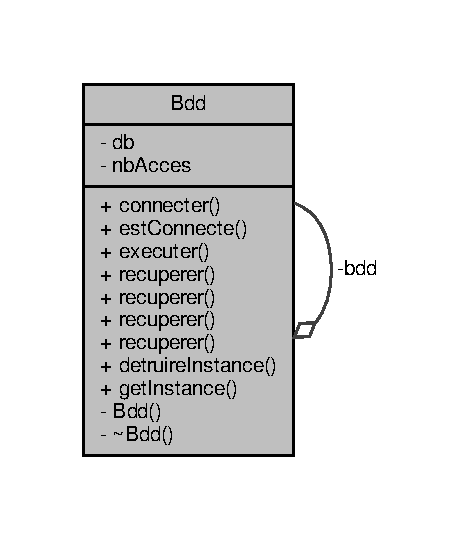
\includegraphics[width=221pt]{class_bdd__coll__graph}
\end{center}
\end{figure}
\subsubsection*{Fonctions membres publiques}
\begin{DoxyCompactItemize}
\item 
bool \hyperlink{class_bdd_a1a234e773787295f521d66685149176b}{connecter} ()
\begin{DoxyCompactList}\small\item\em Définition méthose \hyperlink{class_bdd_a1a234e773787295f521d66685149176b}{connecter()} \end{DoxyCompactList}\item 
bool \hyperlink{class_bdd_afeb7ee6793705cb94a94560fd53e3e9d}{est\+Connecte} ()
\begin{DoxyCompactList}\small\item\em retourne l\textquotesingle{}état de connexion à la base de données \end{DoxyCompactList}\item 
bool \hyperlink{class_bdd_ab6ae645b4b54ce5df8dc9b422fb39faa}{executer} (Q\+String requete)
\begin{DoxyCompactList}\small\item\em exécute une requête S\+QL de type U\+P\+D\+A\+TE, I\+N\+S\+E\+RT et D\+E\+L\+E\+TE \end{DoxyCompactList}\item 
bool \hyperlink{class_bdd_a8f25d29d309041bbf875700db0efd97b}{recuperer} (Q\+String requete, Q\+String \&donnees)
\begin{DoxyCompactList}\small\item\em exécute une requête S\+QL de type S\+E\+L\+E\+CT et récupère un champ d\textquotesingle{}un seul enregistrement \end{DoxyCompactList}\item 
bool \hyperlink{class_bdd_a397b32b8bc612aadf95bf0595e37ec7c}{recuperer} (Q\+String requete, Q\+String\+List \&donnees)
\begin{DoxyCompactList}\small\item\em exécute une requête S\+QL de type S\+E\+L\+E\+CT et récupère plusieurs champs d\textquotesingle{}un seul enregistrement \end{DoxyCompactList}\item 
bool \hyperlink{class_bdd_ae155534b5b1a9daa94ee2106fcf0f37d}{recuperer} (Q\+String requete, Q\+Vector$<$ Q\+String $>$ \&donnees)
\begin{DoxyCompactList}\small\item\em exécute une requête S\+QL de type S\+E\+L\+E\+CT et récupère un seul champ de plusieurs enregistrements \end{DoxyCompactList}\item 
bool \hyperlink{class_bdd_a482cd502a23b933712400044e1ba3e37}{recuperer} (Q\+String requete, Q\+Vector$<$ Q\+String\+List $>$ \&donnees)
\begin{DoxyCompactList}\small\item\em exécute une requête S\+QL de type S\+E\+L\+E\+CT et récupère plusieurs champs de plusieurs enregistrements \end{DoxyCompactList}\end{DoxyCompactItemize}
\subsubsection*{Fonctions membres publiques statiques}
\begin{DoxyCompactItemize}
\item 
static void \hyperlink{class_bdd_af89fa3ffa107c7859a3964bf032cfdb7}{detruire\+Instance} ()
\begin{DoxyCompactList}\small\item\em Définition méthode \hyperlink{class_bdd_af89fa3ffa107c7859a3964bf032cfdb7}{detruire\+Instance()} \end{DoxyCompactList}\item 
static \hyperlink{class_bdd}{Bdd} $\ast$ \hyperlink{class_bdd_a6f55c29d593da12ca31fad02f5adfe24}{get\+Instance} ()
\begin{DoxyCompactList}\small\item\em Définition méthode \hyperlink{class_bdd_a6f55c29d593da12ca31fad02f5adfe24}{get\+Instance()} \end{DoxyCompactList}\end{DoxyCompactItemize}
\subsubsection*{Fonctions membres privées}
\begin{DoxyCompactItemize}
\item 
\hyperlink{class_bdd_a5306aeacb2baa3be8d4d3f8326527f60}{Bdd} ()
\begin{DoxyCompactList}\small\item\em Définition du constructeur de la classe \hyperlink{class_bdd}{Bdd}. \end{DoxyCompactList}\item 
\hyperlink{class_bdd_a5029277f27f8cfcf9d8603fb331a15dd}{$\sim$\+Bdd} ()
\begin{DoxyCompactList}\small\item\em Définition du destructeur de la classe \hyperlink{class_bdd}{Bdd}. \end{DoxyCompactList}\end{DoxyCompactItemize}
\subsubsection*{Attributs privés}
\begin{DoxyCompactItemize}
\item 
Q\+Sql\+Database \hyperlink{class_bdd_a8628c1686deda86999f86689c3e7268e}{db}
\begin{DoxyCompactList}\small\item\em pour la connexion à la base de données My\+S\+QL \end{DoxyCompactList}\end{DoxyCompactItemize}
\subsubsection*{Attributs privés statiques}
\begin{DoxyCompactItemize}
\item 
static \hyperlink{class_bdd}{Bdd} $\ast$ \hyperlink{class_bdd_a09bd3b3a31feedf3dd42a507e0249213}{bdd} = N\+U\+LL
\begin{DoxyCompactList}\small\item\em pointeur sur l\textquotesingle{}instance unique \end{DoxyCompactList}\item 
static int \hyperlink{class_bdd_a9fb6aa118a28c27307f27fd7662e462d}{nb\+Acces} = 0
\begin{DoxyCompactList}\small\item\em compte le nombre d\textquotesingle{}accès à l\textquotesingle{}instance unique \end{DoxyCompactList}\end{DoxyCompactItemize}


\subsubsection{Description détaillée}
Déclaration de la classe utilisant la base de données. 

\begin{DoxyAuthor}{Auteur}
Legger Pierre-\/\+Antoine 

Tranchat Joffrey
\end{DoxyAuthor}
\begin{DoxyVersion}{Version}
1.\+0
\end{DoxyVersion}
\begin{DoxyDate}{Date}
Vendredi 14 Février 
\end{DoxyDate}


Définition à la ligne \hyperlink{_bdd_8h_source_l00042}{42} du fichier \hyperlink{_bdd_8h_source}{Bdd.\+h}.



\subsubsection{Documentation des constructeurs et destructeur}
\mbox{\Hypertarget{class_bdd_a5306aeacb2baa3be8d4d3f8326527f60}\label{class_bdd_a5306aeacb2baa3be8d4d3f8326527f60}} 
\index{Bdd@{Bdd}!Bdd@{Bdd}}
\index{Bdd@{Bdd}!Bdd@{Bdd}}
\paragraph{\texorpdfstring{Bdd()}{Bdd()}}
{\footnotesize\ttfamily Bdd\+::\+Bdd (\begin{DoxyParamCaption}{ }\end{DoxyParamCaption})\hspace{0.3cm}{\ttfamily [private]}}



Définition du constructeur de la classe \hyperlink{class_bdd}{Bdd}. 

initialise le type My\+S\+QL pour la connexion à la base de données 

Définition à la ligne \hyperlink{_bdd_8cpp_source_l00027}{27} du fichier \hyperlink{_bdd_8cpp_source}{Bdd.\+cpp}.



Références \hyperlink{_bdd_8h_source_l00063}{db}.



Référencé par \hyperlink{_bdd_8cpp_source_l00053}{get\+Instance()}.


\begin{DoxyCode}
00028 \{
00029 \textcolor{preprocessor}{    #ifdef DEBUG\_BDD}
00030     qDebug() << Q\_FUNC\_INFO;
00031 \textcolor{preprocessor}{    #endif}
00032     \hyperlink{class_bdd_a8628c1686deda86999f86689c3e7268e}{db} = QSqlDatabase::addDatabase(\textcolor{stringliteral}{"QMYSQL"});
00033 \}
\end{DoxyCode}
\mbox{\Hypertarget{class_bdd_a5029277f27f8cfcf9d8603fb331a15dd}\label{class_bdd_a5029277f27f8cfcf9d8603fb331a15dd}} 
\index{Bdd@{Bdd}!````~Bdd@{$\sim$\+Bdd}}
\index{````~Bdd@{$\sim$\+Bdd}!Bdd@{Bdd}}
\paragraph{\texorpdfstring{$\sim$\+Bdd()}{~Bdd()}}
{\footnotesize\ttfamily Bdd\+::$\sim$\+Bdd (\begin{DoxyParamCaption}{ }\end{DoxyParamCaption})\hspace{0.3cm}{\ttfamily [private]}}



Définition du destructeur de la classe \hyperlink{class_bdd}{Bdd}. 

destructeur de la classe \hyperlink{class_bdd}{Bdd} 

Définition à la ligne \hyperlink{_bdd_8cpp_source_l00040}{40} du fichier \hyperlink{_bdd_8cpp_source}{Bdd.\+cpp}.


\begin{DoxyCode}
00041 \{
00042 \textcolor{preprocessor}{    #ifdef DEBUG\_BDD}
00043     qDebug() << Q\_FUNC\_INFO;
00044 \textcolor{preprocessor}{    #endif}
00045 \}
\end{DoxyCode}


\subsubsection{Documentation des fonctions membres}
\mbox{\Hypertarget{class_bdd_a1a234e773787295f521d66685149176b}\label{class_bdd_a1a234e773787295f521d66685149176b}} 
\index{Bdd@{Bdd}!connecter@{connecter}}
\index{connecter@{connecter}!Bdd@{Bdd}}
\paragraph{\texorpdfstring{connecter()}{connecter()}}
{\footnotesize\ttfamily bool Bdd\+::connecter (\begin{DoxyParamCaption}{ }\end{DoxyParamCaption})}



Définition méthose \hyperlink{class_bdd_a1a234e773787295f521d66685149176b}{connecter()} 

permet de se connecter à la base de données \begin{DoxyReturn}{Renvoie}
boolean 
\end{DoxyReturn}


Définition à la ligne \hyperlink{_bdd_8cpp_source_l00093}{93} du fichier \hyperlink{_bdd_8cpp_source}{Bdd.\+cpp}.



Références \hyperlink{_bdd_8h_source_l00013}{D\+A\+T\+A\+B\+A\+S\+E\+N\+A\+ME}, \hyperlink{_bdd_8h_source_l00063}{db}, \hyperlink{_bdd_8h_source_l00010}{H\+O\+S\+T\+N\+A\+ME}, \hyperlink{_bdd_8h_source_l00012}{P\+A\+S\+S\+W\+O\+RD}, et \hyperlink{_bdd_8h_source_l00011}{U\+S\+E\+R\+N\+A\+ME}.



Référencé par \hyperlink{_supervision_8cpp_source_l00036}{Supervision\+::\+Supervision()}.


\begin{DoxyCode}
00094 \{
00095     \textcolor{keywordflow}{if}(!\hyperlink{class_bdd_a8628c1686deda86999f86689c3e7268e}{db}.isOpen())
00096     \{
00097         \hyperlink{class_bdd_a8628c1686deda86999f86689c3e7268e}{db}.setHostName(\hyperlink{_bdd_8h_a63ebf0552e7b4b8f37af87147904ffce}{HOSTNAME});
00098         \hyperlink{class_bdd_a8628c1686deda86999f86689c3e7268e}{db}.setUserName(\hyperlink{_bdd_8h_a3a747cf18fa28f0de7920de0f89f5144}{USERNAME});
00099         \hyperlink{class_bdd_a8628c1686deda86999f86689c3e7268e}{db}.setPassword(\hyperlink{_bdd_8h_a9e8538fad4eee548302ad9f60e6d47ca}{PASSWORD});
00100         \hyperlink{class_bdd_a8628c1686deda86999f86689c3e7268e}{db}.setDatabaseName(\hyperlink{_bdd_8h_aed52a1560b7fbe28f212643a9be8a139}{DATABASENAME});
00101 
00102 \textcolor{preprocessor}{        #ifdef DEBUG\_BDD}
00103         qDebug() << Q\_FUNC\_INFO << \textcolor{stringliteral}{"HostName"} << \hyperlink{class_bdd_a8628c1686deda86999f86689c3e7268e}{db}.hostName();
00104         qDebug() << Q\_FUNC\_INFO << \textcolor{stringliteral}{"UserName"} << \hyperlink{class_bdd_a8628c1686deda86999f86689c3e7268e}{db}.userName();
00105         qDebug() << Q\_FUNC\_INFO << \textcolor{stringliteral}{"DatabaseName"} << \hyperlink{class_bdd_a8628c1686deda86999f86689c3e7268e}{db}.databaseName();
00106 \textcolor{preprocessor}{        #endif}
00107         \textcolor{keywordflow}{if}(\hyperlink{class_bdd_a8628c1686deda86999f86689c3e7268e}{db}.open())
00108         \{
00109 \textcolor{preprocessor}{            #ifdef DEBUG\_BDD}
00110             qDebug() << Q\_FUNC\_INFO << QString::fromUtf8(\textcolor{stringliteral}{"connexion réussie à %1"}).arg(
      \hyperlink{class_bdd_a8628c1686deda86999f86689c3e7268e}{db}.hostName());
00111 \textcolor{preprocessor}{            #endif}
00112 
00113             \textcolor{keywordflow}{return} \textcolor{keyword}{true};
00114         \}
00115         \textcolor{keywordflow}{else}
00116         \{
00117             qDebug() << Q\_FUNC\_INFO << QString::fromUtf8(\textcolor{stringliteral}{"erreur : impossible de se connecter à la base de
       données !"});
00118 
00119             QMessageBox::critical(0, QString::fromUtf8(\textcolor{stringliteral}{"e-stock"}), QString::fromUtf8(\textcolor{stringliteral}{"Impossible de se
       connecter à la base de données !"}));
00120             \textcolor{keywordflow}{return} \textcolor{keyword}{false};
00121         \}
00122 
00123     \}
00124     \textcolor{keywordflow}{else}
00125         \textcolor{keywordflow}{return} \textcolor{keyword}{true};
00126 \}
\end{DoxyCode}
\mbox{\Hypertarget{class_bdd_af89fa3ffa107c7859a3964bf032cfdb7}\label{class_bdd_af89fa3ffa107c7859a3964bf032cfdb7}} 
\index{Bdd@{Bdd}!detruire\+Instance@{detruire\+Instance}}
\index{detruire\+Instance@{detruire\+Instance}!Bdd@{Bdd}}
\paragraph{\texorpdfstring{detruire\+Instance()}{detruireInstance()}}
{\footnotesize\ttfamily void Bdd\+::detruire\+Instance (\begin{DoxyParamCaption}{ }\end{DoxyParamCaption})\hspace{0.3cm}{\ttfamily [static]}}



Définition méthode \hyperlink{class_bdd_af89fa3ffa107c7859a3964bf032cfdb7}{detruire\+Instance()} 

détruit l\textquotesingle{}instance de la \hyperlink{class_bdd}{Bdd} si elle existe et si personne l\textquotesingle{}utilise 

Définition à la ligne \hyperlink{_bdd_8cpp_source_l00073}{73} du fichier \hyperlink{_bdd_8cpp_source}{Bdd.\+cpp}.



Références \hyperlink{_bdd_8h_source_l00064}{bdd}, et \hyperlink{_bdd_8h_source_l00065}{nb\+Acces}.



Référencé par \hyperlink{_armoire_8cpp_source_l00036}{Armoire\+::$\sim$\+Armoire()}.


\begin{DoxyCode}
00074 \{
00075     \textcolor{keywordflow}{if}(\hyperlink{class_bdd_a09bd3b3a31feedf3dd42a507e0249213}{bdd} != NULL)
00076     \{
00077         \hyperlink{class_bdd_a9fb6aa118a28c27307f27fd7662e462d}{nbAcces}--;
00078 \textcolor{preprocessor}{        #ifdef DEBUG\_BASEDEDONNEES}
00079         qDebug() << Q\_FUNC\_INFO << \textcolor{stringliteral}{"nbAcces"} << \hyperlink{class_bdd_a9fb6aa118a28c27307f27fd7662e462d}{nbAcces};
00080 \textcolor{preprocessor}{        #endif}
00081 
00082         \textcolor{keywordflow}{if}(nbAcces == 0)
00083             \textcolor{keyword}{delete} \hyperlink{class_bdd_a09bd3b3a31feedf3dd42a507e0249213}{bdd};
00084     \}
00085 \}
\end{DoxyCode}
\mbox{\Hypertarget{class_bdd_afeb7ee6793705cb94a94560fd53e3e9d}\label{class_bdd_afeb7ee6793705cb94a94560fd53e3e9d}} 
\index{Bdd@{Bdd}!est\+Connecte@{est\+Connecte}}
\index{est\+Connecte@{est\+Connecte}!Bdd@{Bdd}}
\paragraph{\texorpdfstring{est\+Connecte()}{estConnecte()}}
{\footnotesize\ttfamily bool Bdd\+::est\+Connecte (\begin{DoxyParamCaption}{ }\end{DoxyParamCaption})}



retourne l\textquotesingle{}état de connexion à la base de données 

retourne l\textquotesingle{}état de connexion à la base de données \begin{DoxyReturn}{Renvoie}
boolean true si connecté à la base de données sinon false 
\end{DoxyReturn}


Définition à la ligne \hyperlink{_bdd_8cpp_source_l00134}{134} du fichier \hyperlink{_bdd_8cpp_source}{Bdd.\+cpp}.



Références \hyperlink{_bdd_8h_source_l00063}{db}.


\begin{DoxyCode}
00135 \{
00136     \textcolor{keywordflow}{return} \hyperlink{class_bdd_a8628c1686deda86999f86689c3e7268e}{db}.isOpen();
00137 \}
\end{DoxyCode}
\mbox{\Hypertarget{class_bdd_ab6ae645b4b54ce5df8dc9b422fb39faa}\label{class_bdd_ab6ae645b4b54ce5df8dc9b422fb39faa}} 
\index{Bdd@{Bdd}!executer@{executer}}
\index{executer@{executer}!Bdd@{Bdd}}
\paragraph{\texorpdfstring{executer()}{executer()}}
{\footnotesize\ttfamily bool Bdd\+::executer (\begin{DoxyParamCaption}\item[{Q\+String}]{requete }\end{DoxyParamCaption})}



exécute une requête S\+QL de type U\+P\+D\+A\+TE, I\+N\+S\+E\+RT et D\+E\+L\+E\+TE 

exécute une requête S\+QL de type U\+P\+D\+A\+TE, I\+N\+S\+E\+RT et D\+E\+L\+E\+TE 
\begin{DoxyParams}[1]{Paramètres}
\mbox{\tt in}  & {\em requete} & une requête S\+QL de type U\+P\+D\+A\+TE, I\+N\+S\+E\+RT et D\+E\+L\+E\+TE \\
\hline
\end{DoxyParams}
\begin{DoxyReturn}{Renvoie}
boolean true si la requête a été exécutée avec succès sinon false 
\end{DoxyReturn}


Définition à la ligne \hyperlink{_bdd_8cpp_source_l00146}{146} du fichier \hyperlink{_bdd_8cpp_source}{Bdd.\+cpp}.



Références \hyperlink{_bdd_8h_source_l00063}{db}.



Référencé par \hyperlink{_article_8cpp_source_l00329}{Article\+::mettre\+A\+Jour\+Quantite()}, et \hyperlink{_supervision_8cpp_source_l00141}{Supervision\+::verifier\+Authentification\+Identifiant()}.


\begin{DoxyCode}
00147 \{
00148     QSqlQuery r;
00149     \textcolor{keywordtype}{bool} retour;
00150 
00151     \textcolor{keywordflow}{if}(\hyperlink{class_bdd_a8628c1686deda86999f86689c3e7268e}{db}.isOpen())
00152     \{
00153         \textcolor{keywordflow}{if}(requete.contains(\textcolor{stringliteral}{"UPDATE"}) || requete.contains(\textcolor{stringliteral}{"INSERT"}) || requete.contains(\textcolor{stringliteral}{"DELETE"}))
00154         \{
00155             retour = r.exec(requete);
00156 \textcolor{preprocessor}{            #ifdef DEBUG\_BASEDEDONNEES}
00157             qDebug() << Q\_FUNC\_INFO << QString::fromUtf8(\textcolor{stringliteral}{"Retour %1 pour la requete : %2"}).arg(
      QString::number(retour)).arg(requete);
00158 \textcolor{preprocessor}{            #endif}
00159             \textcolor{keywordflow}{if}(retour)
00160             \{
00161                 \textcolor{keywordflow}{return} \textcolor{keyword}{true};
00162             \}
00163             \textcolor{keywordflow}{else}
00164             \{
00165                 qDebug() << Q\_FUNC\_INFO << QString::fromUtf8(\textcolor{stringliteral}{"Erreur : %1 pour la requête %2"}).arg(r.
      lastError().text()).arg(requete);
00166                 \textcolor{keywordflow}{return} \textcolor{keyword}{false};
00167             \}
00168         \}
00169         \textcolor{keywordflow}{else}
00170         \{
00171             qDebug() << Q\_FUNC\_INFO << QString::fromUtf8(\textcolor{stringliteral}{"Erreur : requête %1 non autorisée !"}).arg(requete
      );
00172             \textcolor{keywordflow}{return} \textcolor{keyword}{false};
00173         \}
00174     \}
00175     \textcolor{keywordflow}{else}
00176         \textcolor{keywordflow}{return} \textcolor{keyword}{false};
00177 
00178 \}
\end{DoxyCode}
\mbox{\Hypertarget{class_bdd_a6f55c29d593da12ca31fad02f5adfe24}\label{class_bdd_a6f55c29d593da12ca31fad02f5adfe24}} 
\index{Bdd@{Bdd}!get\+Instance@{get\+Instance}}
\index{get\+Instance@{get\+Instance}!Bdd@{Bdd}}
\paragraph{\texorpdfstring{get\+Instance()}{getInstance()}}
{\footnotesize\ttfamily \hyperlink{class_bdd}{Bdd} $\ast$ Bdd\+::get\+Instance (\begin{DoxyParamCaption}{ }\end{DoxyParamCaption})\hspace{0.3cm}{\ttfamily [static]}}



Définition méthode \hyperlink{class_bdd_a6f55c29d593da12ca31fad02f5adfe24}{get\+Instance()} 

permet l\textquotesingle{}instanciation d\textquotesingle{}un objet \hyperlink{class_bdd}{Bdd} en vérifiant qu\textquotesingle{}il n\textquotesingle{}en existe pas déja un \begin{DoxyReturn}{Renvoie}
bdd l\textquotesingle{}instance unique 
\end{DoxyReturn}


Définition à la ligne \hyperlink{_bdd_8cpp_source_l00053}{53} du fichier \hyperlink{_bdd_8cpp_source}{Bdd.\+cpp}.



Références \hyperlink{_bdd_8cpp_source_l00027}{Bdd()}, \hyperlink{_bdd_8h_source_l00064}{bdd}, et \hyperlink{_bdd_8h_source_l00065}{nb\+Acces}.



Référencé par \hyperlink{_armoire_8cpp_source_l00022}{Armoire\+::\+Armoire()}, et \hyperlink{_supervision_8cpp_source_l00036}{Supervision\+::\+Supervision()}.


\begin{DoxyCode}
00054 \{
00055     \textcolor{keywordflow}{if}(\hyperlink{class_bdd_a09bd3b3a31feedf3dd42a507e0249213}{bdd} == NULL)
00056         \hyperlink{class_bdd_a09bd3b3a31feedf3dd42a507e0249213}{bdd} = \textcolor{keyword}{new} \hyperlink{class_bdd_a5306aeacb2baa3be8d4d3f8326527f60}{Bdd}();
00057 
00058     \hyperlink{class_bdd_a9fb6aa118a28c27307f27fd7662e462d}{nbAcces}++;
00059 
00060 \textcolor{preprocessor}{    #ifdef DEBUG\_BDD}
00061     qDebug() << Q\_FUNC\_INFO << \textcolor{stringliteral}{"nbAcces"} << \hyperlink{class_bdd_a9fb6aa118a28c27307f27fd7662e462d}{nbAcces};
00062 \textcolor{preprocessor}{    #endif}
00063 
00064     \textcolor{keywordflow}{return} \hyperlink{class_bdd_a09bd3b3a31feedf3dd42a507e0249213}{bdd};
00065 
00066 \}
\end{DoxyCode}
\mbox{\Hypertarget{class_bdd_a8f25d29d309041bbf875700db0efd97b}\label{class_bdd_a8f25d29d309041bbf875700db0efd97b}} 
\index{Bdd@{Bdd}!recuperer@{recuperer}}
\index{recuperer@{recuperer}!Bdd@{Bdd}}
\paragraph{\texorpdfstring{recuperer()}{recuperer()}\hspace{0.1cm}{\footnotesize\ttfamily [1/4]}}
{\footnotesize\ttfamily bool Bdd\+::recuperer (\begin{DoxyParamCaption}\item[{Q\+String}]{requete,  }\item[{Q\+String \&}]{donnees }\end{DoxyParamCaption})}



exécute une requête S\+QL de type S\+E\+L\+E\+CT et récupère un champ d\textquotesingle{}un seul enregistrement 


\begin{DoxyParams}[1]{Paramètres}
\mbox{\tt in}  & {\em requete} & une requête S\+QL de type S\+E\+L\+E\+CT \\
\hline
\mbox{\tt out}  & {\em donnees} & le champ Q\+String récupéré \\
\hline
\end{DoxyParams}
\begin{DoxyReturn}{Renvoie}
boolean true si la requête a été exécutée avec succès sinon false 
\end{DoxyReturn}


Définition à la ligne \hyperlink{_bdd_8cpp_source_l00187}{187} du fichier \hyperlink{_bdd_8cpp_source}{Bdd.\+cpp}.



Références \hyperlink{_bdd_8h_source_l00063}{db}.



Référencé par \hyperlink{_supervision_8cpp_source_l00305}{Supervision\+::rechercher\+Article()}, \hyperlink{_armoire_8cpp_source_l00049}{Armoire\+::recuperer\+Armoire()}, \hyperlink{_article_8cpp_source_l00050}{Article\+::recuperer\+Donnees\+Article()}, \hyperlink{_article_8cpp_source_l00103}{Article\+::recuperer\+Donnees\+Article\+Par\+Nom()}, \hyperlink{_article_8cpp_source_l00156}{Article\+::recuperer\+Donnees\+Article\+Par\+Numero\+Casier()}, \hyperlink{_supervision_8cpp_source_l00165}{Supervision\+::recuperer\+Donnees\+Utilisateur()}, \hyperlink{_article_8cpp_source_l00202}{Article\+::recuperer\+Nombre\+Casiers\+Pour\+Id\+Article()}, \hyperlink{_article_8cpp_source_l00218}{Article\+::recuperer\+Nombre\+Casiers\+Pour\+Nom\+Article()}, \hyperlink{_article_8cpp_source_l00234}{Article\+::recuperer\+Numero\+Casier\+Pour\+Id\+Article()}, et \hyperlink{_article_8cpp_source_l00250}{Article\+::recuperer\+Numero\+Casier\+Pour\+Nom\+Article()}.


\begin{DoxyCode}
00188 \{
00189     QSqlQuery r;
00190     \textcolor{keywordtype}{bool} retour;
00191 
00192     \textcolor{keywordflow}{if}(\hyperlink{class_bdd_a8628c1686deda86999f86689c3e7268e}{db}.isOpen())
00193     \{
00194         \textcolor{keywordflow}{if}(requete.contains(\textcolor{stringliteral}{"SELECT"}))
00195         \{
00196             retour = r.exec(requete);
00197 \textcolor{preprocessor}{            #ifdef DEBUG\_BASEDEDONNEES}
00198             qDebug() << Q\_FUNC\_INFO << QString::fromUtf8(\textcolor{stringliteral}{"Retour %1 pour la requete : %2"}).arg(
      QString::number(retour)).arg(requete);
00199 \textcolor{preprocessor}{            #endif}
00200             \textcolor{keywordflow}{if}(retour)
00201             \{
00202                 \textcolor{comment}{// on se positionne sur l'enregistrement}
00203                 r.first();
00204 
00205                 \textcolor{comment}{// on vérifie l'état de l'enregistrement retourné}
00206                 \textcolor{keywordflow}{if}(!r.isValid())
00207                 \{
00208 \textcolor{preprocessor}{                    #ifdef DEBUG\_BASEDEDONNEES}
00209                     qDebug() << Q\_FUNC\_INFO << QString::fromUtf8(\textcolor{stringliteral}{"Résultat non valide !"});
00210 \textcolor{preprocessor}{                    #endif}
00211                     \textcolor{keywordflow}{return} \textcolor{keyword}{false};
00212                 \}
00213 
00214                 \textcolor{comment}{// on récupère sous forme de QString la valeur du champ}
00215                 \textcolor{keywordflow}{if}(r.isNull(0))
00216                 \{
00217 \textcolor{preprocessor}{                    #ifdef DEBUG\_BASEDEDONNEES}
00218                     qDebug() << Q\_FUNC\_INFO << QString::fromUtf8(\textcolor{stringliteral}{"Aucun résultat !"});
00219 \textcolor{preprocessor}{                    #endif}
00220                     \textcolor{keywordflow}{return} \textcolor{keyword}{false};
00221                 \}
00222                 donnees = r.value(0).toString();
00223 \textcolor{preprocessor}{                #ifdef DEBUG\_BASEDEDONNEES}
00224                 qDebug() << Q\_FUNC\_INFO << \textcolor{stringliteral}{"Enregistrement -> "} << donnees;
00225 \textcolor{preprocessor}{                #endif}
00226                 \textcolor{keywordflow}{return} \textcolor{keyword}{true};
00227             \}
00228             \textcolor{keywordflow}{else}
00229             \{
00230                 qDebug() << Q\_FUNC\_INFO << QString::fromUtf8(\textcolor{stringliteral}{"Erreur : %1 pour la requête %2"}).arg(r.
      lastError().text()).arg(requete);
00231                 \textcolor{keywordflow}{return} \textcolor{keyword}{false};
00232             \}
00233         \}
00234         \textcolor{keywordflow}{else}
00235         \{
00236             qDebug() << Q\_FUNC\_INFO << QString::fromUtf8(\textcolor{stringliteral}{"Erreur : requête %1 non autorisée !"}).arg(requete
      );
00237             \textcolor{keywordflow}{return} \textcolor{keyword}{false};
00238         \}
00239     \}
00240     \textcolor{keywordflow}{else}
00241         \textcolor{keywordflow}{return} \textcolor{keyword}{false};
00242 \}
\end{DoxyCode}
\mbox{\Hypertarget{class_bdd_a397b32b8bc612aadf95bf0595e37ec7c}\label{class_bdd_a397b32b8bc612aadf95bf0595e37ec7c}} 
\index{Bdd@{Bdd}!recuperer@{recuperer}}
\index{recuperer@{recuperer}!Bdd@{Bdd}}
\paragraph{\texorpdfstring{recuperer()}{recuperer()}\hspace{0.1cm}{\footnotesize\ttfamily [2/4]}}
{\footnotesize\ttfamily bool Bdd\+::recuperer (\begin{DoxyParamCaption}\item[{Q\+String}]{requete,  }\item[{Q\+String\+List \&}]{donnees }\end{DoxyParamCaption})}



exécute une requête S\+QL de type S\+E\+L\+E\+CT et récupère plusieurs champs d\textquotesingle{}un seul enregistrement 


\begin{DoxyParams}[1]{Paramètres}
\mbox{\tt in}  & {\em requete} & une requête S\+QL de type S\+E\+L\+E\+CT \\
\hline
\mbox{\tt out}  & {\em donnees} & plusieurs champs d\textquotesingle{}un seul enregistrement dans un Q\+String\+List \\
\hline
\end{DoxyParams}
\begin{DoxyReturn}{Renvoie}
boolean true si la requête a été exécutée avec succès sinon false 
\end{DoxyReturn}


Définition à la ligne \hyperlink{_bdd_8cpp_source_l00251}{251} du fichier \hyperlink{_bdd_8cpp_source}{Bdd.\+cpp}.



Références \hyperlink{_bdd_8h_source_l00063}{db}.


\begin{DoxyCode}
00252 \{
00253     QSqlQuery r;
00254     \textcolor{keywordtype}{bool} retour;
00255 
00256     \textcolor{keywordflow}{if}(\hyperlink{class_bdd_a8628c1686deda86999f86689c3e7268e}{db}.isOpen())
00257     \{
00258         \textcolor{keywordflow}{if}(requete.contains(\textcolor{stringliteral}{"SELECT"}))
00259         \{
00260             retour = r.exec(requete);
00261 \textcolor{preprocessor}{            #ifdef DEBUG\_BASEDEDONNEES}
00262             qDebug() << QString::fromUtf8(\textcolor{stringliteral}{"Retour %1 pour la requete : %2"}).arg(QString::number(retour)).
      arg(requete);
00263 \textcolor{preprocessor}{            #endif}
00264             \textcolor{keywordflow}{if}(retour)
00265             \{
00266                 \textcolor{comment}{// on se positionne sur l'enregistrement}
00267                 r.first();
00268 
00269                 \textcolor{comment}{// on vérifie l'état de l'enregistrement retourné}
00270                 \textcolor{keywordflow}{if}(!r.isValid())
00271                 \{
00272 \textcolor{preprocessor}{                    #ifdef DEBUG\_BASEDEDONNEES}
00273                     qDebug() << Q\_FUNC\_INFO << QString::fromUtf8(\textcolor{stringliteral}{"Résultat non valide !"});
00274 \textcolor{preprocessor}{                    #endif}
00275                     \textcolor{keywordflow}{return} \textcolor{keyword}{false};
00276                 \}
00277 
00278                 \textcolor{comment}{// on récupère sous forme de QString la valeur de tous les champs sélectionnés}
00279                 \textcolor{comment}{// et on les stocke dans une liste de QString}
00280                 \textcolor{keywordflow}{for}(\textcolor{keywordtype}{int} i=0;i<r.record().count();i++)
00281                     \textcolor{keywordflow}{if}(!r.isNull(i))
00282                         donnees << r.value(i).toString();
00283 \textcolor{preprocessor}{                #ifdef DEBUG\_BASEDEDONNEES}
00284                 qDebug() << Q\_FUNC\_INFO << \textcolor{stringliteral}{"Enregistrement -> "} << donnees;
00285 \textcolor{preprocessor}{                #endif}
00286                 \textcolor{keywordflow}{return} \textcolor{keyword}{true};
00287             \}
00288             \textcolor{keywordflow}{else}
00289             \{
00290                 qDebug() << Q\_FUNC\_INFO << QString::fromUtf8(\textcolor{stringliteral}{"Erreur : %1 pour la requête %2"}).arg(r.
      lastError().text()).arg(requete);
00291                 \textcolor{keywordflow}{return} \textcolor{keyword}{false};
00292             \}
00293         \}
00294         \textcolor{keywordflow}{else}
00295         \{
00296             qDebug() << Q\_FUNC\_INFO << QString::fromUtf8(\textcolor{stringliteral}{"Erreur : requête %1 non autorisée !"}).arg(requete
      );
00297             \textcolor{keywordflow}{return} \textcolor{keyword}{false};
00298         \}
00299     \}
00300     \textcolor{keywordflow}{else}
00301         \textcolor{keywordflow}{return} \textcolor{keyword}{false};
00302 \}
\end{DoxyCode}
\mbox{\Hypertarget{class_bdd_ae155534b5b1a9daa94ee2106fcf0f37d}\label{class_bdd_ae155534b5b1a9daa94ee2106fcf0f37d}} 
\index{Bdd@{Bdd}!recuperer@{recuperer}}
\index{recuperer@{recuperer}!Bdd@{Bdd}}
\paragraph{\texorpdfstring{recuperer()}{recuperer()}\hspace{0.1cm}{\footnotesize\ttfamily [3/4]}}
{\footnotesize\ttfamily bool Bdd\+::recuperer (\begin{DoxyParamCaption}\item[{Q\+String}]{requete,  }\item[{Q\+Vector$<$ Q\+String $>$ \&}]{donnees }\end{DoxyParamCaption})}



exécute une requête S\+QL de type S\+E\+L\+E\+CT et récupère un seul champ de plusieurs enregistrements 


\begin{DoxyParams}[1]{Paramètres}
\mbox{\tt in}  & {\em requete} & une requête S\+QL de type S\+E\+L\+E\+CT \\
\hline
\mbox{\tt out}  & {\em donnees} & un seul champ de plusieurs enregistrements dans un Q\+Vector de Q\+String \\
\hline
\end{DoxyParams}
\begin{DoxyReturn}{Renvoie}
boolean true si la requête a été exécutée avec succès sinon false 
\end{DoxyReturn}


Définition à la ligne \hyperlink{_bdd_8cpp_source_l00311}{311} du fichier \hyperlink{_bdd_8cpp_source}{Bdd.\+cpp}.



Références \hyperlink{_bdd_8h_source_l00063}{db}.


\begin{DoxyCode}
00312 \{
00313     QSqlQuery r;
00314     \textcolor{keywordtype}{bool} retour;
00315     QString data;
00316 
00317     \textcolor{keywordflow}{if}(\hyperlink{class_bdd_a8628c1686deda86999f86689c3e7268e}{db}.isOpen())
00318     \{
00319         \textcolor{keywordflow}{if}(requete.contains(\textcolor{stringliteral}{"SELECT"}))
00320         \{
00321             retour = r.exec(requete);
00322 \textcolor{preprocessor}{            #ifdef DEBUG\_BASEDEDONNEES}
00323             qDebug() << Q\_FUNC\_INFO << QString::fromUtf8(\textcolor{stringliteral}{"Retour %1 pour la requete : %2"}).arg(
      QString::number(retour)).arg(requete);
00324 \textcolor{preprocessor}{            #endif}
00325             \textcolor{keywordflow}{if}(retour)
00326             \{
00327                 \textcolor{comment}{// pour chaque enregistrement}
00328                 \textcolor{keywordflow}{while} ( r.next() )
00329                 \{
00330                     \textcolor{comment}{// on récupère sous forme de QString la valeur du champs sélectionné}
00331                     data = r.value(0).toString();
00332 
00333 \textcolor{preprocessor}{                    #ifdef DEBUG\_BASEDEDONNEES}
00334                     \textcolor{comment}{//qDebug() << Q\_FUNC\_INFO << "Enregistrement -> " << data;}
00335 \textcolor{preprocessor}{                    #endif}
00336 
00337                     \textcolor{comment}{// on stocke l'enregistrement dans le QVector}
00338                     donnees.push\_back(data);
00339                 \}
00340 \textcolor{preprocessor}{                #ifdef DEBUG\_BASEDEDONNEES}
00341                 qDebug() << Q\_FUNC\_INFO << \textcolor{stringliteral}{"Enregistrement -> "} << donnees;
00342 \textcolor{preprocessor}{                #endif}
00343                 \textcolor{keywordflow}{return} \textcolor{keyword}{true};
00344             \}
00345             \textcolor{keywordflow}{else}
00346             \{
00347                 qDebug() << Q\_FUNC\_INFO << QString::fromUtf8(\textcolor{stringliteral}{"Erreur : %1 pour la requête %2"}).arg(r.
      lastError().text()).arg(requete);
00348                 \textcolor{keywordflow}{return} \textcolor{keyword}{false};
00349             \}
00350         \}
00351         \textcolor{keywordflow}{else}
00352         \{
00353             qDebug() << Q\_FUNC\_INFO << QString::fromUtf8(\textcolor{stringliteral}{"Erreur : requête %1 non autorisée !"}).arg(requete
      );
00354             \textcolor{keywordflow}{return} \textcolor{keyword}{false};
00355         \}
00356     \}
00357     \textcolor{keywordflow}{else}
00358         \textcolor{keywordflow}{return} \textcolor{keyword}{false};
00359 \}
\end{DoxyCode}
\mbox{\Hypertarget{class_bdd_a482cd502a23b933712400044e1ba3e37}\label{class_bdd_a482cd502a23b933712400044e1ba3e37}} 
\index{Bdd@{Bdd}!recuperer@{recuperer}}
\index{recuperer@{recuperer}!Bdd@{Bdd}}
\paragraph{\texorpdfstring{recuperer()}{recuperer()}\hspace{0.1cm}{\footnotesize\ttfamily [4/4]}}
{\footnotesize\ttfamily bool Bdd\+::recuperer (\begin{DoxyParamCaption}\item[{Q\+String}]{requete,  }\item[{Q\+Vector$<$ Q\+String\+List $>$ \&}]{donnees }\end{DoxyParamCaption})}



exécute une requête S\+QL de type S\+E\+L\+E\+CT et récupère plusieurs champs de plusieurs enregistrements 


\begin{DoxyParams}[1]{Paramètres}
\mbox{\tt in}  & {\em requete} & une requête S\+QL de type S\+E\+L\+E\+CT \\
\hline
\mbox{\tt out}  & {\em donnees} & \+: plusieurs champs de plusieurs enregistrements dans un Q\+Vector de Q\+String\+List \\
\hline
\end{DoxyParams}
\begin{DoxyReturn}{Renvoie}
boolean true si la requête a été exécutée avec succès sinon false 
\end{DoxyReturn}


Définition à la ligne \hyperlink{_bdd_8cpp_source_l00367}{367} du fichier \hyperlink{_bdd_8cpp_source}{Bdd.\+cpp}.



Références \hyperlink{_bdd_8h_source_l00063}{db}.


\begin{DoxyCode}
00368 \{
00369     QSqlQuery r;
00370     \textcolor{keywordtype}{bool} retour;
00371     QStringList data;
00372 
00373     \textcolor{keywordflow}{if}(\hyperlink{class_bdd_a8628c1686deda86999f86689c3e7268e}{db}.isOpen())
00374     \{
00375         \textcolor{keywordflow}{if}(requete.contains(\textcolor{stringliteral}{"SELECT"}))
00376         \{
00377             retour = r.exec(requete);
00378 \textcolor{preprocessor}{            #ifdef DEBUG\_BASEDEDONNEES}
00379             qDebug() << Q\_FUNC\_INFO << QString::fromUtf8(\textcolor{stringliteral}{"Retour %1 pour la requete : %2"}).arg(
      QString::number(retour)).arg(requete);
00380 \textcolor{preprocessor}{            #endif}
00381             \textcolor{keywordflow}{if}(retour)
00382             \{
00383                 \textcolor{comment}{// pour chaque enregistrement}
00384                 \textcolor{keywordflow}{while} ( r.next() )
00385                 \{
00386                     \textcolor{comment}{// on récupère sous forme de QString la valeur de tous les champs sélectionnés}
00387                     \textcolor{comment}{// et on les stocke dans une liste de QString}
00388                     \textcolor{keywordflow}{for}(\textcolor{keywordtype}{int} i=0;i<r.record().count();i++)
00389                         data << r.value(i).toString();
00390 
00391 \textcolor{preprocessor}{                    #ifdef DEBUG\_BASEDEDONNEES}
00392                     \textcolor{comment}{//qDebug() << Q\_FUNC\_INFO << "Enregistrement -> " << data;}
00393                     \textcolor{comment}{/*for(int i=0;i<r.record().count();i++)}
00394 \textcolor{comment}{                        qDebug() << r.value(i).toString();*/}
00395 \textcolor{preprocessor}{                    #endif}
00396 
00397                     \textcolor{comment}{// on stocke l'enregistrement dans le QVector}
00398                     donnees.push\_back(data);
00399 
00400                     \textcolor{comment}{// on efface la liste de QString pour le prochain enregistrement}
00401                     data.clear();
00402                 \}
00403 \textcolor{preprocessor}{                #ifdef DEBUG\_BASEDEDONNEES}
00404                 qDebug() << Q\_FUNC\_INFO << \textcolor{stringliteral}{"Enregistrement -> "} << donnees;
00405 \textcolor{preprocessor}{                #endif}
00406                 \textcolor{keywordflow}{return} \textcolor{keyword}{true};
00407             \}
00408             \textcolor{keywordflow}{else}
00409             \{
00410                 qDebug() << Q\_FUNC\_INFO << QString::fromUtf8(\textcolor{stringliteral}{"Erreur : %1 pour la requête %2"}).arg(r.
      lastError().text()).arg(requete);
00411                 \textcolor{keywordflow}{return} \textcolor{keyword}{false};
00412             \}
00413         \}
00414         \textcolor{keywordflow}{else}
00415         \{
00416             qDebug() << Q\_FUNC\_INFO << QString::fromUtf8(\textcolor{stringliteral}{"Erreur : requête %1 non autorisée !"}).arg(requete
      );
00417             \textcolor{keywordflow}{return} \textcolor{keyword}{false};
00418         \}
00419     \}
00420     \textcolor{keywordflow}{else}
00421         \textcolor{keywordflow}{return} \textcolor{keyword}{false};
00422 \}
\end{DoxyCode}


\subsubsection{Documentation des données membres}
\mbox{\Hypertarget{class_bdd_a09bd3b3a31feedf3dd42a507e0249213}\label{class_bdd_a09bd3b3a31feedf3dd42a507e0249213}} 
\index{Bdd@{Bdd}!bdd@{bdd}}
\index{bdd@{bdd}!Bdd@{Bdd}}
\paragraph{\texorpdfstring{bdd}{bdd}}
{\footnotesize\ttfamily \hyperlink{class_bdd}{Bdd} $\ast$ Bdd\+::bdd = N\+U\+LL\hspace{0.3cm}{\ttfamily [static]}, {\ttfamily [private]}}



pointeur sur l\textquotesingle{}instance unique 



Définition à la ligne \hyperlink{_bdd_8h_source_l00064}{64} du fichier \hyperlink{_bdd_8h_source}{Bdd.\+h}.



Référencé par \hyperlink{_bdd_8cpp_source_l00073}{detruire\+Instance()}, et \hyperlink{_bdd_8cpp_source_l00053}{get\+Instance()}.

\mbox{\Hypertarget{class_bdd_a8628c1686deda86999f86689c3e7268e}\label{class_bdd_a8628c1686deda86999f86689c3e7268e}} 
\index{Bdd@{Bdd}!db@{db}}
\index{db@{db}!Bdd@{Bdd}}
\paragraph{\texorpdfstring{db}{db}}
{\footnotesize\ttfamily Q\+Sql\+Database Bdd\+::db\hspace{0.3cm}{\ttfamily [private]}}



pour la connexion à la base de données My\+S\+QL 



Définition à la ligne \hyperlink{_bdd_8h_source_l00063}{63} du fichier \hyperlink{_bdd_8h_source}{Bdd.\+h}.



Référencé par \hyperlink{_bdd_8cpp_source_l00027}{Bdd()}, \hyperlink{_bdd_8cpp_source_l00093}{connecter()}, \hyperlink{_bdd_8cpp_source_l00134}{est\+Connecte()}, \hyperlink{_bdd_8cpp_source_l00146}{executer()}, et \hyperlink{_bdd_8cpp_source_l00187}{recuperer()}.

\mbox{\Hypertarget{class_bdd_a9fb6aa118a28c27307f27fd7662e462d}\label{class_bdd_a9fb6aa118a28c27307f27fd7662e462d}} 
\index{Bdd@{Bdd}!nb\+Acces@{nb\+Acces}}
\index{nb\+Acces@{nb\+Acces}!Bdd@{Bdd}}
\paragraph{\texorpdfstring{nb\+Acces}{nbAcces}}
{\footnotesize\ttfamily int Bdd\+::nb\+Acces = 0\hspace{0.3cm}{\ttfamily [static]}, {\ttfamily [private]}}



compte le nombre d\textquotesingle{}accès à l\textquotesingle{}instance unique 



Définition à la ligne \hyperlink{_bdd_8h_source_l00065}{65} du fichier \hyperlink{_bdd_8h_source}{Bdd.\+h}.



Référencé par \hyperlink{_bdd_8cpp_source_l00073}{detruire\+Instance()}, et \hyperlink{_bdd_8cpp_source_l00053}{get\+Instance()}.



La documentation de cette classe a été générée à partir des fichiers suivants \+:\begin{DoxyCompactItemize}
\item 
\hyperlink{_bdd_8h}{Bdd.\+h}\item 
\hyperlink{_bdd_8cpp}{Bdd.\+cpp}\end{DoxyCompactItemize}

\hypertarget{class_casier}{}\subsection{Référence de la classe Casier}
\label{class_casier}\index{Casier@{Casier}}


La classe \hyperlink{class_casier}{Casier} gère le casier contenant des articles.  




{\ttfamily \#include $<$Casier.\+h$>$}



Graphe de collaboration de Casier\+:
\nopagebreak
\begin{figure}[H]
\begin{center}
\leavevmode
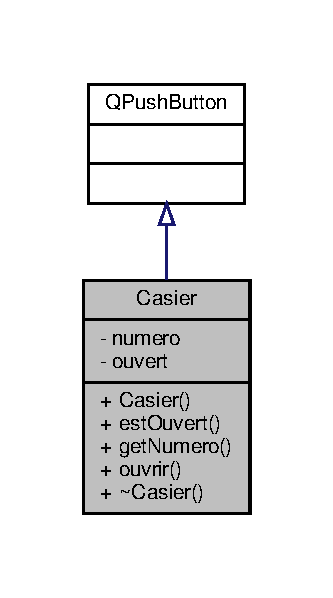
\includegraphics[width=160pt]{class_casier__coll__graph}
\end{center}
\end{figure}
\subsubsection*{Fonctions membres publiques}
\begin{DoxyCompactItemize}
\item 
\hyperlink{class_casier_aed1cd4435ff913a68b69d8119481bb8f}{Casier} (int \hyperlink{class_casier_a17aa23e73b177559266a9fb17f63b812}{numero}, Q\+Widget $\ast$parent=0)
\begin{DoxyCompactList}\small\item\em Définition de la méthode \hyperlink{class_casier}{Casier}. \end{DoxyCompactList}\item 
bool \hyperlink{class_casier_ab26fd4da845423355835da8d445ed5dd}{est\+Ouvert} () const
\begin{DoxyCompactList}\small\item\em Définition de la méthode est\+Ouvert. \end{DoxyCompactList}\item 
int \hyperlink{class_casier_a061b024a2733a5bb1dfcc43bb0022707}{get\+Numero} () const
\begin{DoxyCompactList}\small\item\em Définition de la méthode get\+Numero. \end{DoxyCompactList}\item 
void \hyperlink{class_casier_ac4b0de3ba58dc2bab52b049b278f4f90}{ouvrir} ()
\begin{DoxyCompactList}\small\item\em Définition de la méthode ouvrir. \end{DoxyCompactList}\item 
\hyperlink{class_casier_a4aebc2219ccd4612cf79413904bb9340}{$\sim$\+Casier} ()
\begin{DoxyCompactList}\small\item\em Définition du destructeur de la classe \hyperlink{class_casier}{Casier}. \end{DoxyCompactList}\end{DoxyCompactItemize}
\subsubsection*{Attributs privés}
\begin{DoxyCompactItemize}
\item 
int \hyperlink{class_casier_a17aa23e73b177559266a9fb17f63b812}{numero}
\item 
bool \hyperlink{class_casier_afe544ed1a87ce714a9fbbe16126669e4}{ouvert}
\end{DoxyCompactItemize}


\subsubsection{Description détaillée}
La classe \hyperlink{class_casier}{Casier} gère le casier contenant des articles. 

\begin{DoxyAuthor}{Auteur}
Tranchat Joffrey 

Legger Pierre-\/\+Antoine
\end{DoxyAuthor}
\begin{DoxyVersion}{Version}
1.\+0
\end{DoxyVersion}
\begin{DoxyDate}{Date}
samedi 28 Mars 2020 
\end{DoxyDate}


Définition à la ligne \hyperlink{_casier_8h_source_l00032}{32} du fichier \hyperlink{_casier_8h_source}{Casier.\+h}.



\subsubsection{Documentation des constructeurs et destructeur}
\mbox{\Hypertarget{class_casier_aed1cd4435ff913a68b69d8119481bb8f}\label{class_casier_aed1cd4435ff913a68b69d8119481bb8f}} 
\index{Casier@{Casier}!Casier@{Casier}}
\index{Casier@{Casier}!Casier@{Casier}}
\paragraph{\texorpdfstring{Casier()}{Casier()}}
{\footnotesize\ttfamily Casier\+::\+Casier (\begin{DoxyParamCaption}\item[{int}]{numero,  }\item[{Q\+Widget $\ast$}]{parent = {\ttfamily 0} }\end{DoxyParamCaption})}



Définition de la méthode \hyperlink{class_casier}{Casier}. 


\begin{DoxyParams}{Paramètres}
{\em numero} & \\
\hline
{\em parent} & \\
\hline
\end{DoxyParams}
initialise un objet \hyperlink{class_casier}{Casier} \begin{DoxyRefDesc}{A faire}
\item[\hyperlink{todo__todo000001}{A faire}]Définir une constante pour une taille minimum du casier dans l\textquotesingle{}I\+HM \end{DoxyRefDesc}


\begin{DoxyRefDesc}{A faire}
\item[\hyperlink{todo__todo000002}{A faire}]Gérer les différentes couleurs de fond par rapport à l\textquotesingle{}état (ouvert/fermé, vide, ...) \end{DoxyRefDesc}


\begin{DoxyRefDesc}{A faire}
\item[\hyperlink{todo__todo000003}{A faire}]Connecter signal/slot si nécessaire \end{DoxyRefDesc}


Définition à la ligne \hyperlink{_casier_8cpp_source_l00023}{23} du fichier \hyperlink{_casier_8cpp_source}{Casier.\+cpp}.



Références \hyperlink{_casier_8h_source_l00044}{numero}.


\begin{DoxyCode}
00023                                           : \hyperlink{class_q_push_button}{QPushButton}(parent), 
      \hyperlink{class_casier_a17aa23e73b177559266a9fb17f63b812}{numero}(\hyperlink{class_casier_a17aa23e73b177559266a9fb17f63b812}{numero}), \hyperlink{class_casier_afe544ed1a87ce714a9fbbe16126669e4}{ouvert}(\textcolor{keyword}{false})
00024 \{
00025     qDebug() << Q\_FUNC\_INFO << \hyperlink{class_casier_a17aa23e73b177559266a9fb17f63b812}{numero};
00026     setText(\textcolor{stringliteral}{"Casier "} + QString::number(numero));
00027 
00031     setMaximumHeight(100);
00032     setContentsMargins(10, 0, 10, 0); \textcolor{comment}{// Marges : Gauche Haut Droite Bas}
00036 \textcolor{comment}{}    \textcolor{comment}{//setStyleSheet("background-color: rgb(85, 85, 85);");}
00037     \textcolor{comment}{//setStyleSheet("background-color: rgb(239, 41, 41);");}
00038     setStyleSheet(\textcolor{stringliteral}{"background-color: rgb(115, 210, 22);"});
00039 
00044 \}
\end{DoxyCode}
\mbox{\Hypertarget{class_casier_a4aebc2219ccd4612cf79413904bb9340}\label{class_casier_a4aebc2219ccd4612cf79413904bb9340}} 
\index{Casier@{Casier}!````~Casier@{$\sim$\+Casier}}
\index{````~Casier@{$\sim$\+Casier}!Casier@{Casier}}
\paragraph{\texorpdfstring{$\sim$\+Casier()}{~Casier()}}
{\footnotesize\ttfamily Casier\+::$\sim$\+Casier (\begin{DoxyParamCaption}{ }\end{DoxyParamCaption})}



Définition du destructeur de la classe \hyperlink{class_casier}{Casier}. 

Détruit un objet \hyperlink{class_casier}{Casier} 

Définition à la ligne \hyperlink{_casier_8cpp_source_l00050}{50} du fichier \hyperlink{_casier_8cpp_source}{Casier.\+cpp}.



Références \hyperlink{_casier_8h_source_l00044}{numero}.


\begin{DoxyCode}
00051 \{
00052     qDebug() << Q\_FUNC\_INFO << \hyperlink{class_casier_a17aa23e73b177559266a9fb17f63b812}{numero};
00053 \}
\end{DoxyCode}


\subsubsection{Documentation des fonctions membres}
\mbox{\Hypertarget{class_casier_ab26fd4da845423355835da8d445ed5dd}\label{class_casier_ab26fd4da845423355835da8d445ed5dd}} 
\index{Casier@{Casier}!est\+Ouvert@{est\+Ouvert}}
\index{est\+Ouvert@{est\+Ouvert}!Casier@{Casier}}
\paragraph{\texorpdfstring{est\+Ouvert()}{estOuvert()}}
{\footnotesize\ttfamily bool Casier\+::est\+Ouvert (\begin{DoxyParamCaption}{ }\end{DoxyParamCaption}) const}



Définition de la méthode est\+Ouvert. 

renvoie l\textquotesingle{}état ouvert/fermer du casier \begin{DoxyReturn}{Renvoie}
état du casier 
\end{DoxyReturn}


Définition à la ligne \hyperlink{_casier_8cpp_source_l00070}{70} du fichier \hyperlink{_casier_8cpp_source}{Casier.\+cpp}.



Références \hyperlink{_casier_8h_source_l00045}{ouvert}.


\begin{DoxyCode}
00071 \{
00072     \textcolor{keywordflow}{return} \hyperlink{class_casier_afe544ed1a87ce714a9fbbe16126669e4}{ouvert};
00073 \}
\end{DoxyCode}
\mbox{\Hypertarget{class_casier_a061b024a2733a5bb1dfcc43bb0022707}\label{class_casier_a061b024a2733a5bb1dfcc43bb0022707}} 
\index{Casier@{Casier}!get\+Numero@{get\+Numero}}
\index{get\+Numero@{get\+Numero}!Casier@{Casier}}
\paragraph{\texorpdfstring{get\+Numero()}{getNumero()}}
{\footnotesize\ttfamily int Casier\+::get\+Numero (\begin{DoxyParamCaption}{ }\end{DoxyParamCaption}) const}



Définition de la méthode get\+Numero. 

renvoie le numero du caiser \begin{DoxyReturn}{Renvoie}
numero du casier 
\end{DoxyReturn}


Définition à la ligne \hyperlink{_casier_8cpp_source_l00060}{60} du fichier \hyperlink{_casier_8cpp_source}{Casier.\+cpp}.



Références \hyperlink{_casier_8h_source_l00044}{numero}.



Référencé par \hyperlink{_ihm_8cpp_source_l00087}{Ihm\+::placer\+Casier()}.


\begin{DoxyCode}
00061 \{
00062     \textcolor{keywordflow}{return} \hyperlink{class_casier_a17aa23e73b177559266a9fb17f63b812}{numero};
00063 \}
\end{DoxyCode}
\mbox{\Hypertarget{class_casier_ac4b0de3ba58dc2bab52b049b278f4f90}\label{class_casier_ac4b0de3ba58dc2bab52b049b278f4f90}} 
\index{Casier@{Casier}!ouvrir@{ouvrir}}
\index{ouvrir@{ouvrir}!Casier@{Casier}}
\paragraph{\texorpdfstring{ouvrir()}{ouvrir()}}
{\footnotesize\ttfamily void Casier\+::ouvrir (\begin{DoxyParamCaption}{ }\end{DoxyParamCaption})}



Définition de la méthode ouvrir. 

envoie la trame d\textquotesingle{}ouverture du casier \begin{DoxyRefDesc}{A faire}
\item[\hyperlink{todo__todo000004}{A faire}]Envoyer trame ouverture \end{DoxyRefDesc}


Définition à la ligne \hyperlink{_casier_8cpp_source_l00079}{79} du fichier \hyperlink{_casier_8cpp_source}{Casier.\+cpp}.


\begin{DoxyCode}
00080 \{
00084 \}
\end{DoxyCode}


\subsubsection{Documentation des données membres}
\mbox{\Hypertarget{class_casier_a17aa23e73b177559266a9fb17f63b812}\label{class_casier_a17aa23e73b177559266a9fb17f63b812}} 
\index{Casier@{Casier}!numero@{numero}}
\index{numero@{numero}!Casier@{Casier}}
\paragraph{\texorpdfstring{numero}{numero}}
{\footnotesize\ttfamily int Casier\+::numero\hspace{0.3cm}{\ttfamily [private]}}



Définition à la ligne \hyperlink{_casier_8h_source_l00044}{44} du fichier \hyperlink{_casier_8h_source}{Casier.\+h}.



Référencé par \hyperlink{_casier_8cpp_source_l00023}{Casier()}, \hyperlink{_casier_8cpp_source_l00060}{get\+Numero()}, et \hyperlink{_casier_8cpp_source_l00050}{$\sim$\+Casier()}.

\mbox{\Hypertarget{class_casier_afe544ed1a87ce714a9fbbe16126669e4}\label{class_casier_afe544ed1a87ce714a9fbbe16126669e4}} 
\index{Casier@{Casier}!ouvert@{ouvert}}
\index{ouvert@{ouvert}!Casier@{Casier}}
\paragraph{\texorpdfstring{ouvert}{ouvert}}
{\footnotesize\ttfamily bool Casier\+::ouvert\hspace{0.3cm}{\ttfamily [private]}}



Définition à la ligne \hyperlink{_casier_8h_source_l00045}{45} du fichier \hyperlink{_casier_8h_source}{Casier.\+h}.



Référencé par \hyperlink{_casier_8cpp_source_l00070}{est\+Ouvert()}.



La documentation de cette classe a été générée à partir des fichiers suivants \+:\begin{DoxyCompactItemize}
\item 
\hyperlink{_casier_8h}{Casier.\+h}\item 
\hyperlink{_casier_8cpp}{Casier.\+cpp}\end{DoxyCompactItemize}

\hypertarget{class_code_barre}{}\subsection{Référence de la classe Code\+Barre}
\label{class_code_barre}\index{Code\+Barre@{Code\+Barre}}


Déclaration de la classe \hyperlink{class_code_barre}{Code\+Barre}.  




{\ttfamily \#include $<$Code\+Barre.\+h$>$}



Graphe de collaboration de Code\+Barre\+:
\nopagebreak
\begin{figure}[H]
\begin{center}
\leavevmode
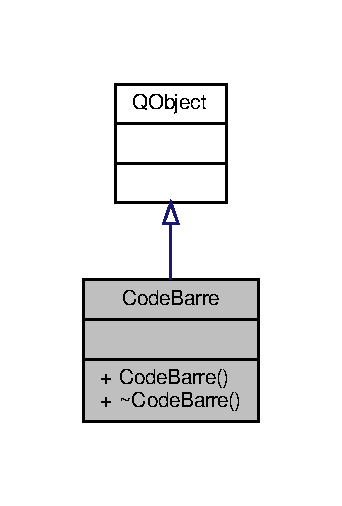
\includegraphics[width=164pt]{class_code_barre__coll__graph}
\end{center}
\end{figure}
\subsubsection*{Fonctions membres publiques}
\begin{DoxyCompactItemize}
\item 
\hyperlink{class_code_barre_a8134bef083f6fa0e01c848d5edd83754}{Code\+Barre} (\hyperlink{class_q_object}{Q\+Object} $\ast$parent=nullptr)
\begin{DoxyCompactList}\small\item\em Définition du constructeur de la classe Code\+Bare. \end{DoxyCompactList}\item 
\hyperlink{class_code_barre_a5bb3df2e5c7fba829f0274da4c359f6c}{$\sim$\+Code\+Barre} ()
\begin{DoxyCompactList}\small\item\em Définition du destructeur de la classe Code\+Bare. \end{DoxyCompactList}\end{DoxyCompactItemize}


\subsubsection{Description détaillée}
Déclaration de la classe \hyperlink{class_code_barre}{Code\+Barre}. 

\begin{DoxyAuthor}{Auteur}
Tranchat Joffrey
\end{DoxyAuthor}
\begin{DoxyVersion}{Version}
1.\+0
\end{DoxyVersion}
\begin{DoxyDate}{Date}
Mercredi 12 Février 2020 
\end{DoxyDate}


Définition à la ligne \hyperlink{_code_barre_8h_source_l00031}{31} du fichier \hyperlink{_code_barre_8h_source}{Code\+Barre.\+h}.



\subsubsection{Documentation des constructeurs et destructeur}
\mbox{\Hypertarget{class_code_barre_a8134bef083f6fa0e01c848d5edd83754}\label{class_code_barre_a8134bef083f6fa0e01c848d5edd83754}} 
\index{Code\+Barre@{Code\+Barre}!Code\+Barre@{Code\+Barre}}
\index{Code\+Barre@{Code\+Barre}!Code\+Barre@{Code\+Barre}}
\paragraph{\texorpdfstring{Code\+Barre()}{CodeBarre()}}
{\footnotesize\ttfamily Code\+Barre\+::\+Code\+Barre (\begin{DoxyParamCaption}\item[{\hyperlink{class_q_object}{Q\+Object} $\ast$}]{parent = {\ttfamily nullptr} }\end{DoxyParamCaption})}



Définition du constructeur de la classe Code\+Bare. 


\begin{DoxyParams}{Paramètres}
{\em parent} & \\
\hline
\end{DoxyParams}
initialise un objet \hyperlink{class_code_barre}{Code\+Barre} 

Définition à la ligne \hyperlink{_code_barre_8cpp_source_l00021}{21} du fichier \hyperlink{_code_barre_8cpp_source}{Code\+Barre.\+cpp}.


\begin{DoxyCode}
00021                                     : \hyperlink{class_q_object}{QObject}(parent)
00022 \{
00023 
00024 \}
\end{DoxyCode}
\mbox{\Hypertarget{class_code_barre_a5bb3df2e5c7fba829f0274da4c359f6c}\label{class_code_barre_a5bb3df2e5c7fba829f0274da4c359f6c}} 
\index{Code\+Barre@{Code\+Barre}!````~Code\+Barre@{$\sim$\+Code\+Barre}}
\index{````~Code\+Barre@{$\sim$\+Code\+Barre}!Code\+Barre@{Code\+Barre}}
\paragraph{\texorpdfstring{$\sim$\+Code\+Barre()}{~CodeBarre()}}
{\footnotesize\ttfamily Code\+Barre\+::$\sim$\+Code\+Barre (\begin{DoxyParamCaption}{ }\end{DoxyParamCaption})}



Définition du destructeur de la classe Code\+Bare. 

Détruit un objet \hyperlink{class_code_barre}{Code\+Barre} 

Définition à la ligne \hyperlink{_code_barre_8cpp_source_l00030}{30} du fichier \hyperlink{_code_barre_8cpp_source}{Code\+Barre.\+cpp}.


\begin{DoxyCode}
00031 \{
00032 
00033 \}
\end{DoxyCode}


La documentation de cette classe a été générée à partir des fichiers suivants \+:\begin{DoxyCompactItemize}
\item 
\hyperlink{_code_barre_8h}{Code\+Barre.\+h}\item 
\hyperlink{_code_barre_8cpp}{Code\+Barre.\+cpp}\end{DoxyCompactItemize}

\hypertarget{class_communication}{}\subsection{Référence de la classe Communication}
\label{class_communication}\index{Communication@{Communication}}


La classe \hyperlink{class_communication}{Communication} permet de communiquer avec le port série.  




{\ttfamily \#include $<$Communication.\+h$>$}



Graphe de collaboration de Communication\+:
\nopagebreak
\begin{figure}[H]
\begin{center}
\leavevmode
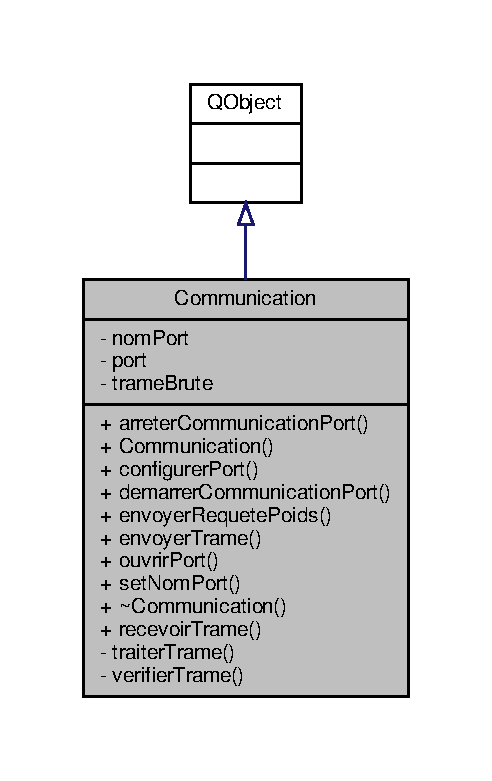
\includegraphics[width=236pt]{class_communication__coll__graph}
\end{center}
\end{figure}
\subsubsection*{Connecteurs publics}
\begin{DoxyCompactItemize}
\item 
void \hyperlink{class_communication_a0b8edc96112e71e1ec4a28cc6309cbbc}{recevoir\+Trame} ()
\begin{DoxyCompactList}\small\item\em Définition de la méthode recevoir\+Trame. \end{DoxyCompactList}\end{DoxyCompactItemize}
\subsubsection*{Signaux}
\begin{DoxyCompactItemize}
\item 
void \hyperlink{class_communication_a8beb7417ede75d0056b06788ef72d21b}{envoie\+Trame\+Etat} (Q\+String trame)
\item 
void \hyperlink{class_communication_a9fb098f5b5cb8931efefc58984529119}{envoie\+Trame\+Ouverture} (Q\+String trame)
\item 
void \hyperlink{class_communication_aaea5653e8aa1b50b4774caf65db21409}{envoie\+Trame\+Poids} (Q\+String trame)
\end{DoxyCompactItemize}
\subsubsection*{Fonctions membres publiques}
\begin{DoxyCompactItemize}
\item 
void \hyperlink{class_communication_aa447a2fe9e2e5c2467a0816865a77340}{arreter\+Communication\+Port} ()
\begin{DoxyCompactList}\small\item\em Définition de la méthode arreter\+Communication\+Port. \end{DoxyCompactList}\item 
\hyperlink{class_communication_a56cf4b262e592bcae1d987c3dd00487f}{Communication} (\hyperlink{class_q_object}{Q\+Object} $\ast$parent=nullptr)
\begin{DoxyCompactList}\small\item\em Constructeur de la classe \hyperlink{class_communication}{Communication}. \end{DoxyCompactList}\item 
void \hyperlink{class_communication_ae39284eac0920a3d11c085b48c6234da}{configurer\+Port} ()
\begin{DoxyCompactList}\small\item\em Définition de la méthode configurer\+Port. \end{DoxyCompactList}\item 
void \hyperlink{class_communication_a8fe8d15efd2590a1061a015f5f761924}{demarrer\+Communication\+Port} ()
\begin{DoxyCompactList}\small\item\em Définition de la méthode demarrer\+Communication\+Port. \end{DoxyCompactList}\item 
void \hyperlink{class_communication_ab8f5efe1d44805be0081e986b2687a12}{envoyer\+Requete\+Poids} (Q\+String numero\+Casier=0)
\begin{DoxyCompactList}\small\item\em Définition de la méthode envoyer\+Requete\+Poids. \end{DoxyCompactList}\item 
void \hyperlink{class_communication_a53c26abe4c16ff155a15929dd5ad07cf}{envoyer\+Trame} (Q\+String trame)
\begin{DoxyCompactList}\small\item\em Définition de la méthode envoyer\+Trame. \end{DoxyCompactList}\item 
void \hyperlink{class_communication_ad5969603a6b7232d0227a461fd479251}{ouvrir\+Port} ()
\begin{DoxyCompactList}\small\item\em Définition de la métohde ouvrir\+Port. \end{DoxyCompactList}\item 
void \hyperlink{class_communication_a06a0f05f4555c6e3586e1800bbaa5e13}{set\+Nom\+Port} (Q\+String nouveau\+Port\+Serie)
\begin{DoxyCompactList}\small\item\em Définition de la méthode set\+Nom\+Port. \end{DoxyCompactList}\item 
\hyperlink{class_communication_a75ba08ce908d45251e28e4c1db94e6f4}{$\sim$\+Communication} ()
\begin{DoxyCompactList}\small\item\em Destructeur de la classe \hyperlink{class_communication}{Communication}. \end{DoxyCompactList}\end{DoxyCompactItemize}
\subsubsection*{Fonctions membres privées}
\begin{DoxyCompactItemize}
\item 
void \hyperlink{class_communication_ab4ff84d0fb69ffa990bc61939c95a093}{traiter\+Trame} (Q\+String trame)
\begin{DoxyCompactList}\small\item\em Définition de la méthode Traiter\+Trame. \end{DoxyCompactList}\item 
bool \hyperlink{class_communication_a3958c8f275ff8d50dca85afe65c795d1}{verifier\+Trame} (Q\+String trame)
\begin{DoxyCompactList}\small\item\em Définition de la méthode verifier\+Trame. \end{DoxyCompactList}\end{DoxyCompactItemize}
\subsubsection*{Attributs privés}
\begin{DoxyCompactItemize}
\item 
Q\+String \hyperlink{class_communication_a5fa89ee1fc732871f3f8f177fb50bf2a}{nom\+Port}
\begin{DoxyCompactList}\small\item\em Variable qui contient le nom du port serie. \end{DoxyCompactList}\item 
Q\+Serial\+Port $\ast$ \hyperlink{class_communication_aff7d55208f31232fbdc1dcec488908f1}{port}
\begin{DoxyCompactList}\small\item\em Variable pointeur sur le port. \end{DoxyCompactList}\item 
Q\+String \hyperlink{class_communication_a7a55775be5e16249315fe5faef4f13b4}{trame\+Brute}
\begin{DoxyCompactList}\small\item\em Variable qui contient la trame brute. \end{DoxyCompactList}\end{DoxyCompactItemize}


\subsubsection{Description détaillée}
La classe \hyperlink{class_communication}{Communication} permet de communiquer avec le port série. 

\begin{DoxyAuthor}{Auteur}
Tranchat Joffrey 

Legger Pierre-\/\+Antoine
\end{DoxyAuthor}
\begin{DoxyVersion}{Version}
1.\+0
\end{DoxyVersion}
\begin{DoxyDate}{Date}
jeudi 12 Mars 2020 
\end{DoxyDate}


Définition à la ligne \hyperlink{_communication_8h_source_l00046}{46} du fichier \hyperlink{_communication_8h_source}{Communication.\+h}.



\subsubsection{Documentation des constructeurs et destructeur}
\mbox{\Hypertarget{class_communication_a56cf4b262e592bcae1d987c3dd00487f}\label{class_communication_a56cf4b262e592bcae1d987c3dd00487f}} 
\index{Communication@{Communication}!Communication@{Communication}}
\index{Communication@{Communication}!Communication@{Communication}}
\paragraph{\texorpdfstring{Communication()}{Communication()}}
{\footnotesize\ttfamily Communication\+::\+Communication (\begin{DoxyParamCaption}\item[{\hyperlink{class_q_object}{Q\+Object} $\ast$}]{parent = {\ttfamily nullptr} }\end{DoxyParamCaption})}



Constructeur de la classe \hyperlink{class_communication}{Communication}. 

initialise un objet \hyperlink{class_communication}{Communication} 
\begin{DoxyParams}{Paramètres}
{\em parent} & \\
\hline
\end{DoxyParams}


Définition à la ligne \hyperlink{_communication_8cpp_source_l00023}{23} du fichier \hyperlink{_communication_8cpp_source}{Communication.\+cpp}.


\begin{DoxyCode}
00023                                             : \hyperlink{class_q_object}{QObject}(parent), \hyperlink{class_communication_aff7d55208f31232fbdc1dcec488908f1}{port}(\textcolor{keyword}{new} QSerialPort(\textcolor{keyword}{this})), 
      \hyperlink{class_communication_a7a55775be5e16249315fe5faef4f13b4}{trameBrute}(\textcolor{stringliteral}{"\(\backslash\)0"}), \hyperlink{class_communication_a5fa89ee1fc732871f3f8f177fb50bf2a}{nomPort}(\hyperlink{_communication_8h_a8542e30f71d5d41f405c329f0e9bafd7}{SERIAL\_PORT\_NAME})
00024 \{
00025     qDebug() << Q\_FUNC\_INFO;
00026 \}
\end{DoxyCode}
\mbox{\Hypertarget{class_communication_a75ba08ce908d45251e28e4c1db94e6f4}\label{class_communication_a75ba08ce908d45251e28e4c1db94e6f4}} 
\index{Communication@{Communication}!````~Communication@{$\sim$\+Communication}}
\index{````~Communication@{$\sim$\+Communication}!Communication@{Communication}}
\paragraph{\texorpdfstring{$\sim$\+Communication()}{~Communication()}}
{\footnotesize\ttfamily Communication\+::$\sim$\+Communication (\begin{DoxyParamCaption}{ }\end{DoxyParamCaption})}



Destructeur de la classe \hyperlink{class_communication}{Communication}. 

Détruit uun objet \hyperlink{class_communication}{Communication} et ferme le port série 

Définition à la ligne \hyperlink{_communication_8cpp_source_l00032}{32} du fichier \hyperlink{_communication_8cpp_source}{Communication.\+cpp}.



Références \hyperlink{_communication_8h_source_l00067}{port}.


\begin{DoxyCode}
00033 \{
00034     \hyperlink{class_communication_aff7d55208f31232fbdc1dcec488908f1}{port}->close();
00035     qDebug() << Q\_FUNC\_INFO;
00036 \}
\end{DoxyCode}


\subsubsection{Documentation des fonctions membres}
\mbox{\Hypertarget{class_communication_aa447a2fe9e2e5c2467a0816865a77340}\label{class_communication_aa447a2fe9e2e5c2467a0816865a77340}} 
\index{Communication@{Communication}!arreter\+Communication\+Port@{arreter\+Communication\+Port}}
\index{arreter\+Communication\+Port@{arreter\+Communication\+Port}!Communication@{Communication}}
\paragraph{\texorpdfstring{arreter\+Communication\+Port()}{arreterCommunicationPort()}}
{\footnotesize\ttfamily void Communication\+::arreter\+Communication\+Port (\begin{DoxyParamCaption}{ }\end{DoxyParamCaption})}



Définition de la méthode arreter\+Communication\+Port. 

Méthode qui ferme le port série 

Définition à la ligne \hyperlink{_communication_8cpp_source_l00053}{53} du fichier \hyperlink{_communication_8cpp_source}{Communication.\+cpp}.



Références \hyperlink{_communication_8h_source_l00067}{port}.


\begin{DoxyCode}
00054 \{
00055     qDebug() << Q\_FUNC\_INFO;
00056     \hyperlink{class_communication_aff7d55208f31232fbdc1dcec488908f1}{port}->close();
00057 \}
\end{DoxyCode}
\mbox{\Hypertarget{class_communication_ae39284eac0920a3d11c085b48c6234da}\label{class_communication_ae39284eac0920a3d11c085b48c6234da}} 
\index{Communication@{Communication}!configurer\+Port@{configurer\+Port}}
\index{configurer\+Port@{configurer\+Port}!Communication@{Communication}}
\paragraph{\texorpdfstring{configurer\+Port()}{configurerPort()}}
{\footnotesize\ttfamily void Communication\+::configurer\+Port (\begin{DoxyParamCaption}{ }\end{DoxyParamCaption})}



Définition de la méthode configurer\+Port. 

Méthode qui configure le port serie par défaut 

Définition à la ligne \hyperlink{_communication_8cpp_source_l00063}{63} du fichier \hyperlink{_communication_8cpp_source}{Communication.\+cpp}.



Références \hyperlink{_communication_8h_source_l00069}{nom\+Port}, et \hyperlink{_communication_8h_source_l00067}{port}.



Référencé par \hyperlink{_communication_8cpp_source_l00042}{demarrer\+Communication\+Port()}.


\begin{DoxyCode}
00064 \{
00065     qDebug() << Q\_FUNC\_INFO;
00066     \hyperlink{class_communication_aff7d55208f31232fbdc1dcec488908f1}{port}->setPortName(\hyperlink{class_communication_a5fa89ee1fc732871f3f8f177fb50bf2a}{nomPort});
00067     \hyperlink{class_communication_aff7d55208f31232fbdc1dcec488908f1}{port}->setBaudRate(QSerialPort::Baud9600);
00068     \hyperlink{class_communication_aff7d55208f31232fbdc1dcec488908f1}{port}->setDataBits(QSerialPort::Data8);
00069     \hyperlink{class_communication_aff7d55208f31232fbdc1dcec488908f1}{port}->setParity(QSerialPort::NoParity);
00070     \hyperlink{class_communication_aff7d55208f31232fbdc1dcec488908f1}{port}->setStopBits(QSerialPort::OneStop);
00071     \hyperlink{class_communication_aff7d55208f31232fbdc1dcec488908f1}{port}->setFlowControl(QSerialPort::NoFlowControl);
00072 \}
\end{DoxyCode}
\mbox{\Hypertarget{class_communication_a8fe8d15efd2590a1061a015f5f761924}\label{class_communication_a8fe8d15efd2590a1061a015f5f761924}} 
\index{Communication@{Communication}!demarrer\+Communication\+Port@{demarrer\+Communication\+Port}}
\index{demarrer\+Communication\+Port@{demarrer\+Communication\+Port}!Communication@{Communication}}
\paragraph{\texorpdfstring{demarrer\+Communication\+Port()}{demarrerCommunicationPort()}}
{\footnotesize\ttfamily void Communication\+::demarrer\+Communication\+Port (\begin{DoxyParamCaption}{ }\end{DoxyParamCaption})}



Définition de la méthode demarrer\+Communication\+Port. 

Méthode qui démarre la configuration du port serie et ouvre le port serie 

Définition à la ligne \hyperlink{_communication_8cpp_source_l00042}{42} du fichier \hyperlink{_communication_8cpp_source}{Communication.\+cpp}.



Références \hyperlink{_communication_8cpp_source_l00063}{configurer\+Port()}, et \hyperlink{_communication_8cpp_source_l00078}{ouvrir\+Port()}.



Référencé par \hyperlink{_supervision_8cpp_source_l00036}{Supervision\+::\+Supervision()}.


\begin{DoxyCode}
00043 \{
00044     qDebug() << Q\_FUNC\_INFO;
00045     \hyperlink{class_communication_ae39284eac0920a3d11c085b48c6234da}{configurerPort}();
00046     \hyperlink{class_communication_ad5969603a6b7232d0227a461fd479251}{ouvrirPort}();
00047 \}
\end{DoxyCode}
\mbox{\Hypertarget{class_communication_a8beb7417ede75d0056b06788ef72d21b}\label{class_communication_a8beb7417ede75d0056b06788ef72d21b}} 
\index{Communication@{Communication}!envoie\+Trame\+Etat@{envoie\+Trame\+Etat}}
\index{envoie\+Trame\+Etat@{envoie\+Trame\+Etat}!Communication@{Communication}}
\paragraph{\texorpdfstring{envoie\+Trame\+Etat}{envoieTrameEtat}}
{\footnotesize\ttfamily void Communication\+::envoie\+Trame\+Etat (\begin{DoxyParamCaption}\item[{Q\+String}]{trame }\end{DoxyParamCaption})\hspace{0.3cm}{\ttfamily [signal]}}



Référencé par \hyperlink{_communication_8cpp_source_l00158}{traiter\+Trame()}.

\mbox{\Hypertarget{class_communication_a9fb098f5b5cb8931efefc58984529119}\label{class_communication_a9fb098f5b5cb8931efefc58984529119}} 
\index{Communication@{Communication}!envoie\+Trame\+Ouverture@{envoie\+Trame\+Ouverture}}
\index{envoie\+Trame\+Ouverture@{envoie\+Trame\+Ouverture}!Communication@{Communication}}
\paragraph{\texorpdfstring{envoie\+Trame\+Ouverture}{envoieTrameOuverture}}
{\footnotesize\ttfamily void Communication\+::envoie\+Trame\+Ouverture (\begin{DoxyParamCaption}\item[{Q\+String}]{trame }\end{DoxyParamCaption})\hspace{0.3cm}{\ttfamily [signal]}}



Référencé par \hyperlink{_communication_8cpp_source_l00158}{traiter\+Trame()}.

\mbox{\Hypertarget{class_communication_aaea5653e8aa1b50b4774caf65db21409}\label{class_communication_aaea5653e8aa1b50b4774caf65db21409}} 
\index{Communication@{Communication}!envoie\+Trame\+Poids@{envoie\+Trame\+Poids}}
\index{envoie\+Trame\+Poids@{envoie\+Trame\+Poids}!Communication@{Communication}}
\paragraph{\texorpdfstring{envoie\+Trame\+Poids}{envoieTramePoids}}
{\footnotesize\ttfamily void Communication\+::envoie\+Trame\+Poids (\begin{DoxyParamCaption}\item[{Q\+String}]{trame }\end{DoxyParamCaption})\hspace{0.3cm}{\ttfamily [signal]}}



Référencé par \hyperlink{_communication_8cpp_source_l00158}{traiter\+Trame()}.

\mbox{\Hypertarget{class_communication_ab8f5efe1d44805be0081e986b2687a12}\label{class_communication_ab8f5efe1d44805be0081e986b2687a12}} 
\index{Communication@{Communication}!envoyer\+Requete\+Poids@{envoyer\+Requete\+Poids}}
\index{envoyer\+Requete\+Poids@{envoyer\+Requete\+Poids}!Communication@{Communication}}
\paragraph{\texorpdfstring{envoyer\+Requete\+Poids()}{envoyerRequetePoids()}}
{\footnotesize\ttfamily void Communication\+::envoyer\+Requete\+Poids (\begin{DoxyParamCaption}\item[{Q\+String}]{numero\+Casier = {\ttfamily 0} }\end{DoxyParamCaption})}



Définition de la méthode envoyer\+Requete\+Poids. 

Méthode qui permet d\textquotesingle{}envoyer une requête pour peser un casier 
\begin{DoxyParams}{Paramètres}
{\em numero\+Casier} & \\
\hline
\end{DoxyParams}


Définition à la ligne \hyperlink{_communication_8cpp_source_l00179}{179} du fichier \hyperlink{_communication_8cpp_source}{Communication.\+cpp}.



Références \hyperlink{_communication_8cpp_source_l00107}{envoyer\+Trame()}.



Référencé par \hyperlink{_supervision_8cpp_source_l00036}{Supervision\+::\+Supervision()}.


\begin{DoxyCode}
00180 \{
00181     QString trame = \textcolor{stringliteral}{"CASIERS;3;"} + numeroCasier + \textcolor{stringliteral}{";\(\backslash\)r\(\backslash\)n"};
00182     \hyperlink{class_communication_a53c26abe4c16ff155a15929dd5ad07cf}{envoyerTrame}(trame);
00183 \}
\end{DoxyCode}
\mbox{\Hypertarget{class_communication_a53c26abe4c16ff155a15929dd5ad07cf}\label{class_communication_a53c26abe4c16ff155a15929dd5ad07cf}} 
\index{Communication@{Communication}!envoyer\+Trame@{envoyer\+Trame}}
\index{envoyer\+Trame@{envoyer\+Trame}!Communication@{Communication}}
\paragraph{\texorpdfstring{envoyer\+Trame()}{envoyerTrame()}}
{\footnotesize\ttfamily void Communication\+::envoyer\+Trame (\begin{DoxyParamCaption}\item[{Q\+String}]{trame }\end{DoxyParamCaption})}



Définition de la méthode envoyer\+Trame. 

Méthode qui permet d\textquotesingle{}envoyer une trame via le port série 
\begin{DoxyParams}{Paramètres}
{\em trame} & \\
\hline
\end{DoxyParams}


Définition à la ligne \hyperlink{_communication_8cpp_source_l00107}{107} du fichier \hyperlink{_communication_8cpp_source}{Communication.\+cpp}.



Références \hyperlink{_communication_8h_source_l00067}{port}.



Référencé par \hyperlink{_communication_8cpp_source_l00179}{envoyer\+Requete\+Poids()}.


\begin{DoxyCode}
00108 \{
00109     \textcolor{keywordflow}{if} (\hyperlink{class_communication_aff7d55208f31232fbdc1dcec488908f1}{port}->isOpen())
00110     \{
00111        \hyperlink{class_communication_aff7d55208f31232fbdc1dcec488908f1}{port}->write(trame.toLatin1());
00112     \}
00113 \}
\end{DoxyCode}
\mbox{\Hypertarget{class_communication_ad5969603a6b7232d0227a461fd479251}\label{class_communication_ad5969603a6b7232d0227a461fd479251}} 
\index{Communication@{Communication}!ouvrir\+Port@{ouvrir\+Port}}
\index{ouvrir\+Port@{ouvrir\+Port}!Communication@{Communication}}
\paragraph{\texorpdfstring{ouvrir\+Port()}{ouvrirPort()}}
{\footnotesize\ttfamily void Communication\+::ouvrir\+Port (\begin{DoxyParamCaption}{ }\end{DoxyParamCaption})}



Définition de la métohde ouvrir\+Port. 

Méthode qui ouvre le port serie en lecture et écriture 

Définition à la ligne \hyperlink{_communication_8cpp_source_l00078}{78} du fichier \hyperlink{_communication_8cpp_source}{Communication.\+cpp}.



Références \hyperlink{_communication_8h_source_l00069}{nom\+Port}, \hyperlink{_communication_8h_source_l00067}{port}, et \hyperlink{_communication_8cpp_source_l00119}{recevoir\+Trame()}.



Référencé par \hyperlink{_communication_8cpp_source_l00042}{demarrer\+Communication\+Port()}.


\begin{DoxyCode}
00079 \{
00080     \textcolor{keywordflow}{if} (\hyperlink{class_communication_aff7d55208f31232fbdc1dcec488908f1}{port}->open(QIODevice::ReadWrite))
00081     \{
00082         qDebug() << Q\_FUNC\_INFO << \textcolor{stringliteral}{"connecté au port"} << \hyperlink{class_communication_a5fa89ee1fc732871f3f8f177fb50bf2a}{nomPort};
00083         connect(\hyperlink{class_communication_aff7d55208f31232fbdc1dcec488908f1}{port}, SIGNAL(readyRead()), \textcolor{keyword}{this}, SLOT(\hyperlink{class_communication_a0b8edc96112e71e1ec4a28cc6309cbbc}{recevoirTrame}()));
00084     \}
00085     \textcolor{keywordflow}{else}
00086     \{
00087         qDebug() << Q\_FUNC\_INFO << \textcolor{stringliteral}{"erreur ouverture du port"} << \hyperlink{class_communication_aff7d55208f31232fbdc1dcec488908f1}{port}->error();
00088     \}
00089 \}
\end{DoxyCode}
\mbox{\Hypertarget{class_communication_a0b8edc96112e71e1ec4a28cc6309cbbc}\label{class_communication_a0b8edc96112e71e1ec4a28cc6309cbbc}} 
\index{Communication@{Communication}!recevoir\+Trame@{recevoir\+Trame}}
\index{recevoir\+Trame@{recevoir\+Trame}!Communication@{Communication}}
\paragraph{\texorpdfstring{recevoir\+Trame}{recevoirTrame}}
{\footnotesize\ttfamily void Communication\+::recevoir\+Trame (\begin{DoxyParamCaption}{ }\end{DoxyParamCaption})\hspace{0.3cm}{\ttfamily [slot]}}



Définition de la méthode recevoir\+Trame. 

Méthode qui permet de recevoir une trame via le port série 

Définition à la ligne \hyperlink{_communication_8cpp_source_l00119}{119} du fichier \hyperlink{_communication_8cpp_source}{Communication.\+cpp}.



Références \hyperlink{_communication_8h_source_l00067}{port}, \hyperlink{_communication_8cpp_source_l00158}{traiter\+Trame()}, \hyperlink{_communication_8h_source_l00068}{trame\+Brute}, et \hyperlink{_communication_8cpp_source_l00138}{verifier\+Trame()}.



Référencé par \hyperlink{_communication_8cpp_source_l00078}{ouvrir\+Port()}.


\begin{DoxyCode}
00120 \{
00121     \hyperlink{class_communication_a7a55775be5e16249315fe5faef4f13b4}{trameBrute} = \textcolor{stringliteral}{"\(\backslash\)0"};
00122 
00123     \textcolor{keywordflow}{while} (\hyperlink{class_communication_aff7d55208f31232fbdc1dcec488908f1}{port}->waitForReadyRead(500))
00124     \{
00125         \hyperlink{class_communication_a7a55775be5e16249315fe5faef4f13b4}{trameBrute}.append(\hyperlink{class_communication_aff7d55208f31232fbdc1dcec488908f1}{port}->readAll());
00126     \}    
00127 
00128     \textcolor{keywordflow}{if}(\hyperlink{class_communication_a3958c8f275ff8d50dca85afe65c795d1}{verifierTrame}(\hyperlink{class_communication_a7a55775be5e16249315fe5faef4f13b4}{trameBrute}))
00129         \hyperlink{class_communication_ab4ff84d0fb69ffa990bc61939c95a093}{traiterTrame}(\hyperlink{class_communication_a7a55775be5e16249315fe5faef4f13b4}{trameBrute});
00130 \}
\end{DoxyCode}
\mbox{\Hypertarget{class_communication_a06a0f05f4555c6e3586e1800bbaa5e13}\label{class_communication_a06a0f05f4555c6e3586e1800bbaa5e13}} 
\index{Communication@{Communication}!set\+Nom\+Port@{set\+Nom\+Port}}
\index{set\+Nom\+Port@{set\+Nom\+Port}!Communication@{Communication}}
\paragraph{\texorpdfstring{set\+Nom\+Port()}{setNomPort()}}
{\footnotesize\ttfamily void Communication\+::set\+Nom\+Port (\begin{DoxyParamCaption}\item[{Q\+String}]{nouveau\+Port\+Serie }\end{DoxyParamCaption})}



Définition de la méthode set\+Nom\+Port. 

Méthode qui permet de définir le nom du port série à utiliser 
\begin{DoxyParams}{Paramètres}
{\em nouveau\+Port\+Serie} & \\
\hline
\end{DoxyParams}


Définition à la ligne \hyperlink{_communication_8cpp_source_l00096}{96} du fichier \hyperlink{_communication_8cpp_source}{Communication.\+cpp}.



Références \hyperlink{_communication_8h_source_l00069}{nom\+Port}.


\begin{DoxyCode}
00097 \{
00098     \hyperlink{class_communication_a5fa89ee1fc732871f3f8f177fb50bf2a}{nomPort} = nouveauPortSerie;
00099     qDebug() << Q\_FUNC\_INFO << \hyperlink{class_communication_a5fa89ee1fc732871f3f8f177fb50bf2a}{nomPort};
00100 \}
\end{DoxyCode}
\mbox{\Hypertarget{class_communication_ab4ff84d0fb69ffa990bc61939c95a093}\label{class_communication_ab4ff84d0fb69ffa990bc61939c95a093}} 
\index{Communication@{Communication}!traiter\+Trame@{traiter\+Trame}}
\index{traiter\+Trame@{traiter\+Trame}!Communication@{Communication}}
\paragraph{\texorpdfstring{traiter\+Trame()}{traiterTrame()}}
{\footnotesize\ttfamily void Communication\+::traiter\+Trame (\begin{DoxyParamCaption}\item[{Q\+String}]{trame }\end{DoxyParamCaption})\hspace{0.3cm}{\ttfamily [private]}}



Définition de la méthode Traiter\+Trame. 

Méthode qui signale le type de trame reçue 
\begin{DoxyParams}{Paramètres}
{\em trame} & \\
\hline
\end{DoxyParams}


Définition à la ligne \hyperlink{_communication_8cpp_source_l00158}{158} du fichier \hyperlink{_communication_8cpp_source}{Communication.\+cpp}.



Références \hyperlink{_communication_8h_source_l00026}{D\+E\+L\+I\+M\+I\+T\+E\+U\+R\+\_\+\+C\+H\+A\+MP}, \hyperlink{_communication_8h_source_l00025}{E\+N\+\_\+\+T\+E\+TE}, \hyperlink{class_communication_a8beb7417ede75d0056b06788ef72d21b}{envoie\+Trame\+Etat()}, \hyperlink{class_communication_a9fb098f5b5cb8931efefc58984529119}{envoie\+Trame\+Ouverture()}, \hyperlink{class_communication_aaea5653e8aa1b50b4774caf65db21409}{envoie\+Trame\+Poids()}, \hyperlink{_communication_8h_source_l00031}{T\+R\+A\+M\+E\+\_\+\+E\+T\+AT}, \hyperlink{_communication_8h_source_l00030}{T\+R\+A\+M\+E\+\_\+\+O\+U\+V\+E\+R\+T\+U\+RE}, et \hyperlink{_communication_8h_source_l00032}{T\+R\+A\+M\+E\+\_\+\+P\+O\+I\+DS}.



Référencé par \hyperlink{_communication_8cpp_source_l00119}{recevoir\+Trame()}.


\begin{DoxyCode}
00159 \{
00160     \textcolor{keywordflow}{if}(trame.startsWith(\hyperlink{_communication_8h_add7c72d962d885317215f93ae8a9dc28}{EN\_TETE} + \hyperlink{_communication_8h_ac3d2c8b3b9dbc07cedf0bfa8a75d268f}{DELIMITEUR\_CHAMP} + 
      \hyperlink{_communication_8h_ad49128d4b2d459f0d7f057b2e59fb2d5}{TRAME\_OUVERTURE} + \hyperlink{_communication_8h_ac3d2c8b3b9dbc07cedf0bfa8a75d268f}{DELIMITEUR\_CHAMP}))
00161     \{
00162         emit \hyperlink{class_communication_a9fb098f5b5cb8931efefc58984529119}{envoieTrameOuverture}(trame);
00163     \}
00164     \textcolor{keywordflow}{else} \textcolor{keywordflow}{if}(trame.startsWith(\hyperlink{_communication_8h_add7c72d962d885317215f93ae8a9dc28}{EN\_TETE} + \hyperlink{_communication_8h_ac3d2c8b3b9dbc07cedf0bfa8a75d268f}{DELIMITEUR\_CHAMP} + 
      \hyperlink{_communication_8h_a57c2e74056a9338d26f264703e2158d8}{TRAME\_ETAT} + \hyperlink{_communication_8h_ac3d2c8b3b9dbc07cedf0bfa8a75d268f}{DELIMITEUR\_CHAMP}))
00165     \{
00166         emit \hyperlink{class_communication_a8beb7417ede75d0056b06788ef72d21b}{envoieTrameEtat}(trame);
00167     \}
00168     \textcolor{keywordflow}{else} \textcolor{keywordflow}{if}(trame.startsWith(\hyperlink{_communication_8h_add7c72d962d885317215f93ae8a9dc28}{EN\_TETE} + \hyperlink{_communication_8h_ac3d2c8b3b9dbc07cedf0bfa8a75d268f}{DELIMITEUR\_CHAMP} + 
      \hyperlink{_communication_8h_a3a24fc54a5e48cb3eb9786ce61933a6c}{TRAME\_POIDS} + \hyperlink{_communication_8h_ac3d2c8b3b9dbc07cedf0bfa8a75d268f}{DELIMITEUR\_CHAMP}))
00169     \{
00170         emit \hyperlink{class_communication_aaea5653e8aa1b50b4774caf65db21409}{envoieTramePoids}(trame);
00171     \}
00172 \}
\end{DoxyCode}
\mbox{\Hypertarget{class_communication_a3958c8f275ff8d50dca85afe65c795d1}\label{class_communication_a3958c8f275ff8d50dca85afe65c795d1}} 
\index{Communication@{Communication}!verifier\+Trame@{verifier\+Trame}}
\index{verifier\+Trame@{verifier\+Trame}!Communication@{Communication}}
\paragraph{\texorpdfstring{verifier\+Trame()}{verifierTrame()}}
{\footnotesize\ttfamily bool Communication\+::verifier\+Trame (\begin{DoxyParamCaption}\item[{Q\+String}]{trame }\end{DoxyParamCaption})\hspace{0.3cm}{\ttfamily [private]}}



Définition de la méthode verifier\+Trame. 

Méthode qui vérifie si la trame respecte le protocole 
\begin{DoxyParams}{Paramètres}
{\em trame} & \\
\hline
\end{DoxyParams}
\begin{DoxyReturn}{Renvoie}
un booleen qui indique si la trame est correct ou nom 
\end{DoxyReturn}


Définition à la ligne \hyperlink{_communication_8cpp_source_l00138}{138} du fichier \hyperlink{_communication_8cpp_source}{Communication.\+cpp}.



Références \hyperlink{_communication_8h_source_l00027}{D\+E\+L\+I\+M\+I\+T\+E\+U\+R\+\_\+\+F\+IN}, et \hyperlink{_communication_8h_source_l00025}{E\+N\+\_\+\+T\+E\+TE}.



Référencé par \hyperlink{_communication_8cpp_source_l00119}{recevoir\+Trame()}.


\begin{DoxyCode}
00139 \{
00140     qDebug() << Q\_FUNC\_INFO << trame;
00141     \textcolor{keywordflow}{if}(!trame.startsWith(\hyperlink{_communication_8h_add7c72d962d885317215f93ae8a9dc28}{EN\_TETE}))
00142     \{
00143         \textcolor{keywordflow}{return} \textcolor{keyword}{false};
00144     \}
00145     \textcolor{keywordflow}{if}(!trame.endsWith(\hyperlink{_communication_8h_aafcc0c7b4996f7783c9f4e766a233487}{DELIMITEUR\_FIN}))
00146     \{
00147         \textcolor{keywordflow}{return} \textcolor{keyword}{false};
00148     \}
00149 
00150     \textcolor{keywordflow}{return} \textcolor{keyword}{true};
00151 \}
\end{DoxyCode}


\subsubsection{Documentation des données membres}
\mbox{\Hypertarget{class_communication_a5fa89ee1fc732871f3f8f177fb50bf2a}\label{class_communication_a5fa89ee1fc732871f3f8f177fb50bf2a}} 
\index{Communication@{Communication}!nom\+Port@{nom\+Port}}
\index{nom\+Port@{nom\+Port}!Communication@{Communication}}
\paragraph{\texorpdfstring{nom\+Port}{nomPort}}
{\footnotesize\ttfamily Q\+String Communication\+::nom\+Port\hspace{0.3cm}{\ttfamily [private]}}



Variable qui contient le nom du port serie. 



Définition à la ligne \hyperlink{_communication_8h_source_l00069}{69} du fichier \hyperlink{_communication_8h_source}{Communication.\+h}.



Référencé par \hyperlink{_communication_8cpp_source_l00063}{configurer\+Port()}, \hyperlink{_communication_8cpp_source_l00078}{ouvrir\+Port()}, et \hyperlink{_communication_8cpp_source_l00096}{set\+Nom\+Port()}.

\mbox{\Hypertarget{class_communication_aff7d55208f31232fbdc1dcec488908f1}\label{class_communication_aff7d55208f31232fbdc1dcec488908f1}} 
\index{Communication@{Communication}!port@{port}}
\index{port@{port}!Communication@{Communication}}
\paragraph{\texorpdfstring{port}{port}}
{\footnotesize\ttfamily Q\+Serial\+Port$\ast$ Communication\+::port\hspace{0.3cm}{\ttfamily [private]}}



Variable pointeur sur le port. 



Définition à la ligne \hyperlink{_communication_8h_source_l00067}{67} du fichier \hyperlink{_communication_8h_source}{Communication.\+h}.



Référencé par \hyperlink{_communication_8cpp_source_l00053}{arreter\+Communication\+Port()}, \hyperlink{_communication_8cpp_source_l00063}{configurer\+Port()}, \hyperlink{_communication_8cpp_source_l00107}{envoyer\+Trame()}, \hyperlink{_communication_8cpp_source_l00078}{ouvrir\+Port()}, \hyperlink{_communication_8cpp_source_l00119}{recevoir\+Trame()}, et \hyperlink{_communication_8cpp_source_l00032}{$\sim$\+Communication()}.

\mbox{\Hypertarget{class_communication_a7a55775be5e16249315fe5faef4f13b4}\label{class_communication_a7a55775be5e16249315fe5faef4f13b4}} 
\index{Communication@{Communication}!trame\+Brute@{trame\+Brute}}
\index{trame\+Brute@{trame\+Brute}!Communication@{Communication}}
\paragraph{\texorpdfstring{trame\+Brute}{trameBrute}}
{\footnotesize\ttfamily Q\+String Communication\+::trame\+Brute\hspace{0.3cm}{\ttfamily [private]}}



Variable qui contient la trame brute. 



Définition à la ligne \hyperlink{_communication_8h_source_l00068}{68} du fichier \hyperlink{_communication_8h_source}{Communication.\+h}.



Référencé par \hyperlink{_communication_8cpp_source_l00119}{recevoir\+Trame()}.



La documentation de cette classe a été générée à partir des fichiers suivants \+:\begin{DoxyCompactItemize}
\item 
\hyperlink{_communication_8h}{Communication.\+h}\item 
\hyperlink{_communication_8cpp}{Communication.\+cpp}\end{DoxyCompactItemize}

\hypertarget{class_ihm}{}\subsection{Référence de la classe Ihm}
\label{class_ihm}\index{Ihm@{Ihm}}


Déclaration de la classe \hyperlink{class_ihm}{Ihm}.  




{\ttfamily \#include $<$Ihm.\+h$>$}



Graphe de collaboration de Ihm\+:
\nopagebreak
\begin{figure}[H]
\begin{center}
\leavevmode
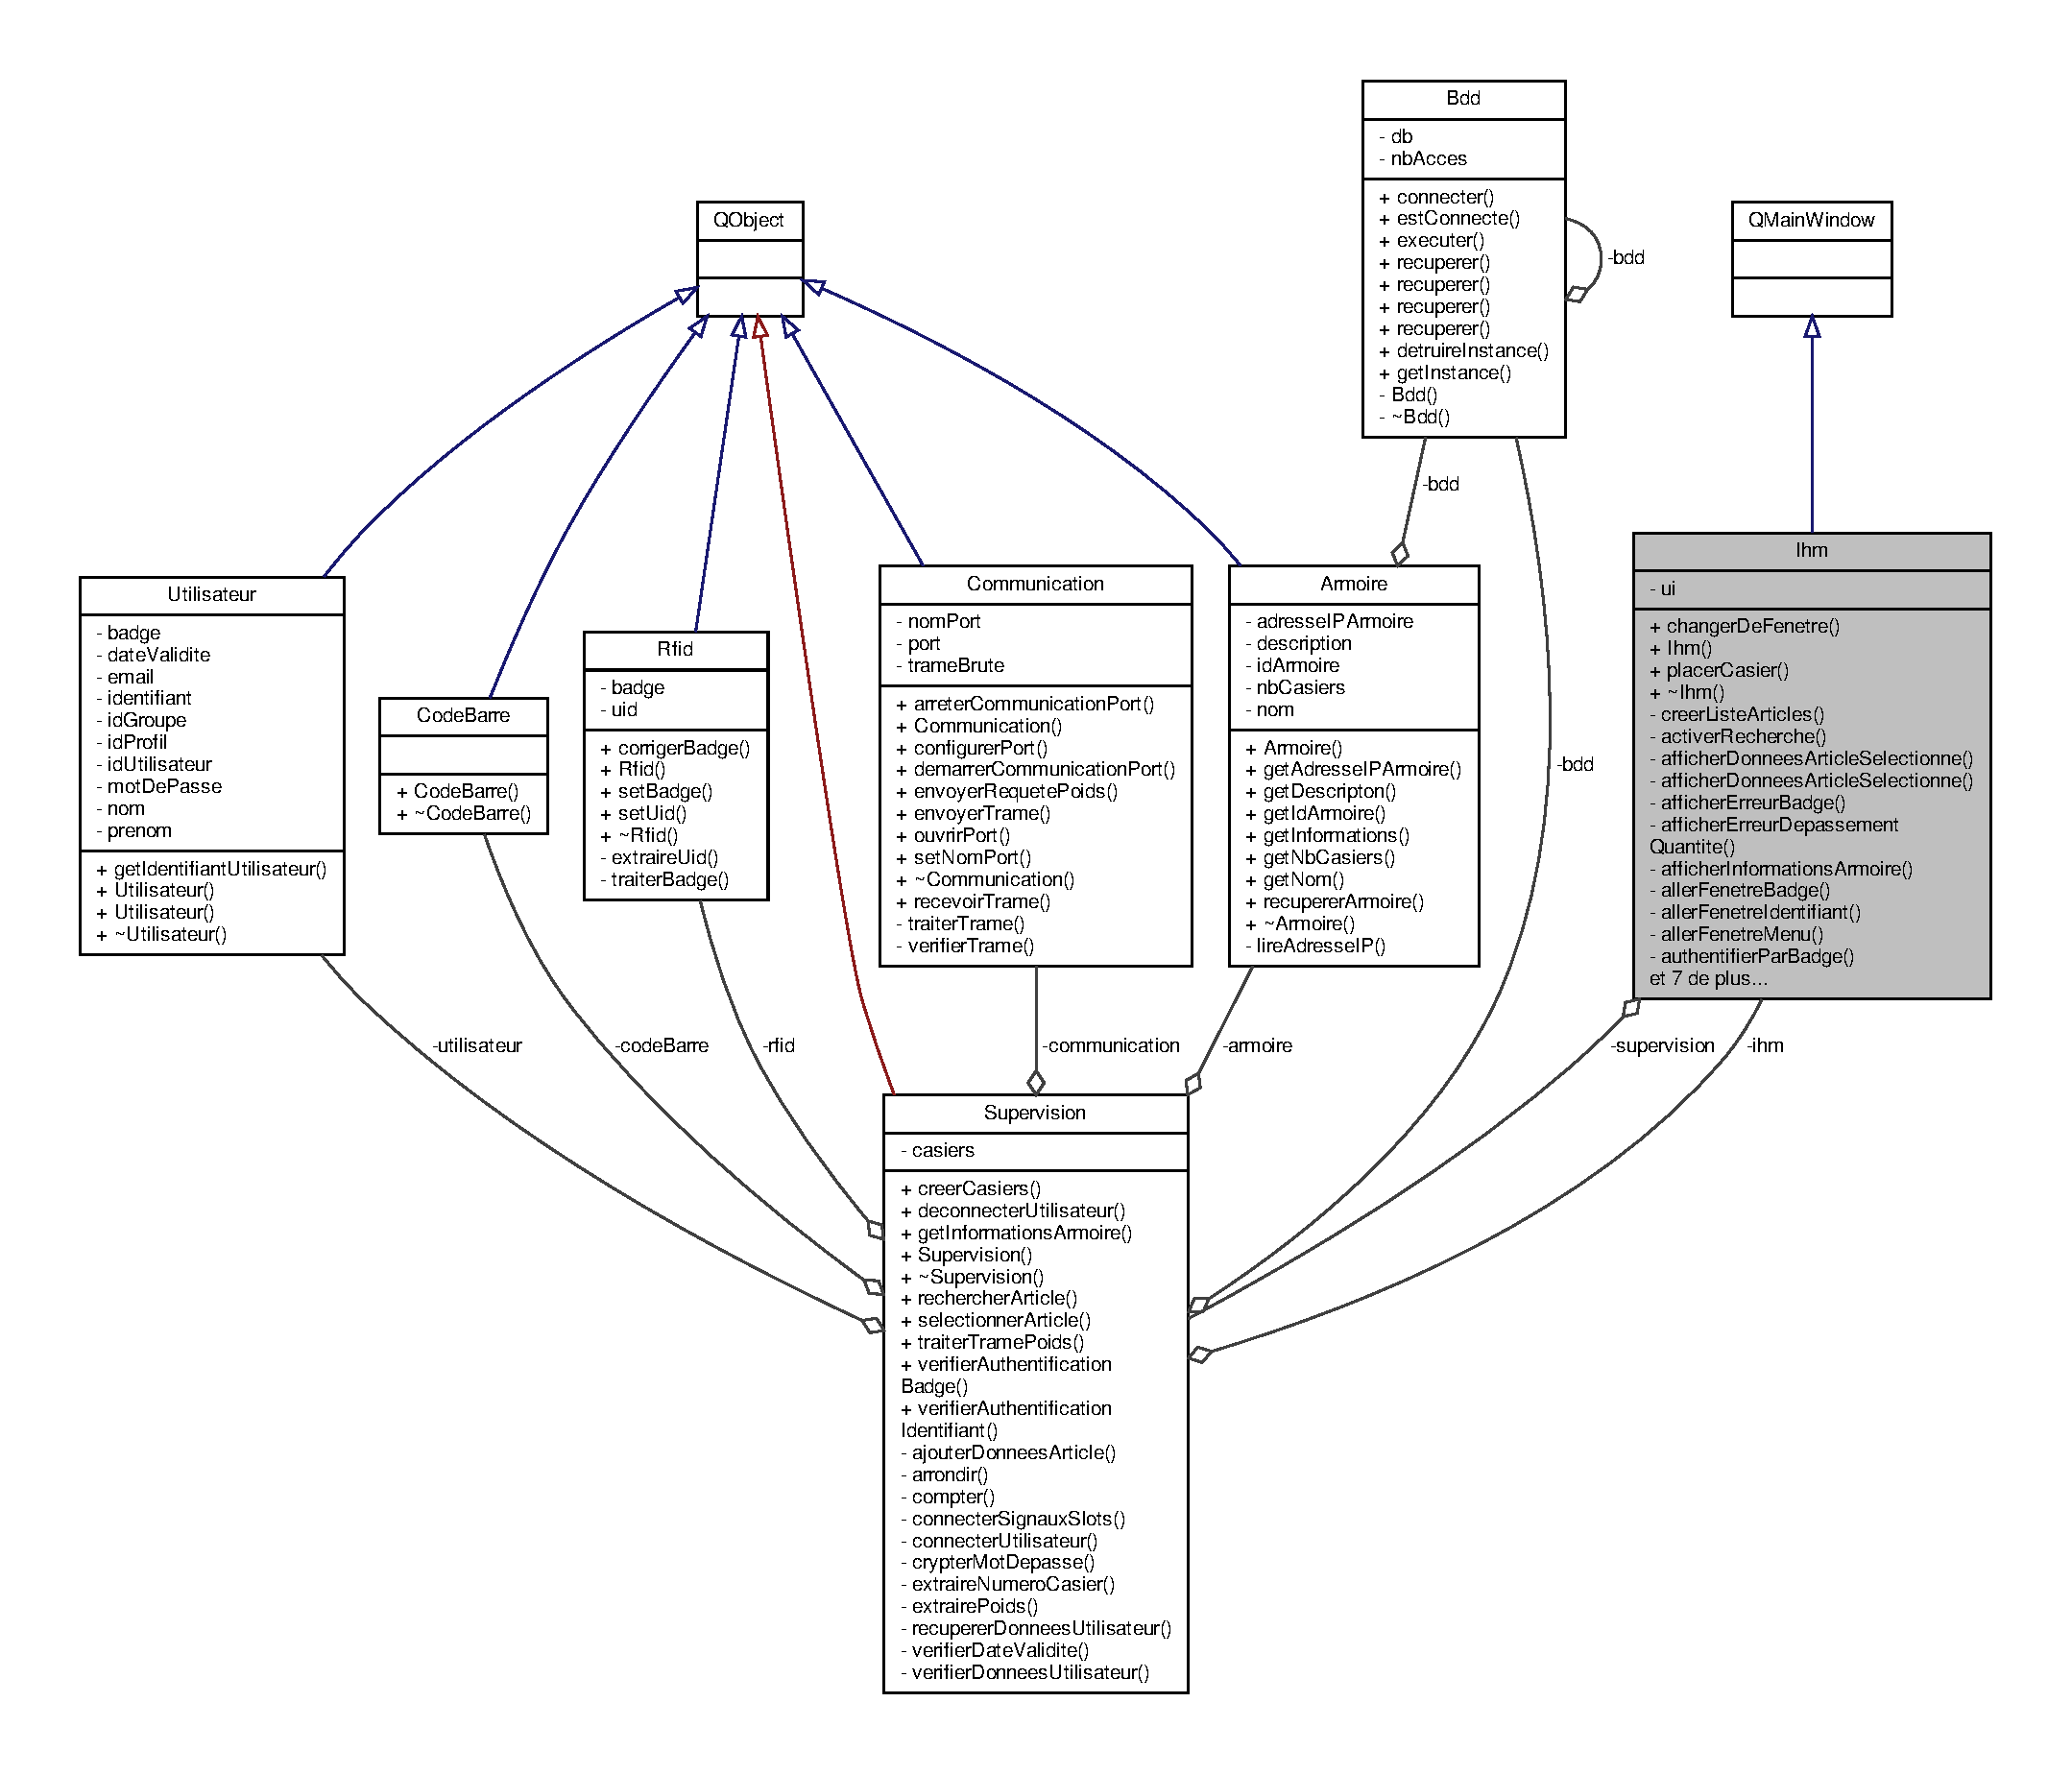
\includegraphics[width=350pt]{class_ihm__coll__graph}
\end{center}
\end{figure}
\subsubsection*{Signaux}
\begin{DoxyCompactItemize}
\item 
void \hyperlink{class_ihm_aef14440b8cc3c9ec92289199ecb7c32f}{article\+Selectionne} (Q\+String)
\item 
void \hyperlink{class_ihm_a15daf0d4cd7c9afd6c97788e54328133}{badge\+Detecte} (Q\+String)
\item 
void \hyperlink{class_ihm_a7cbb2cb835ec643c0a673082d2956405}{identifiant\+Detecte} (Q\+String identifiant, Q\+String mot\+De\+Passe)
\item 
void \hyperlink{class_ihm_a3805ec42b0de42e9210b9561b08f3ecd}{recherche\+Article} (Q\+String)
\end{DoxyCompactItemize}
\subsubsection*{Fonctions membres publiques}
\begin{DoxyCompactItemize}
\item 
void \hyperlink{class_ihm_ab33d5d0a85d60a8d41bae11c34435d50}{changer\+De\+Fenetre} (int fenetre)
\begin{DoxyCompactList}\small\item\em Définition de la méthode changer\+De\+Fenetre. \end{DoxyCompactList}\item 
\hyperlink{class_ihm_a50a7a15775452923868348bdbe4fa51e}{Ihm} (Q\+Widget $\ast$parent=nullptr)
\begin{DoxyCompactList}\small\item\em Constructeur de la classe \hyperlink{class_ihm}{Ihm}. \end{DoxyCompactList}\item 
void \hyperlink{class_ihm_a4ba75b0606c75d616dab3afd67660fd4}{placer\+Casier} (\hyperlink{class_casier}{Casier} $\ast$casier)
\begin{DoxyCompactList}\small\item\em Définition de la méthode placer\+Casier. \end{DoxyCompactList}\item 
\hyperlink{class_ihm_add292ea9005bacd1de44dd1ed9ede5b9}{$\sim$\+Ihm} ()
\begin{DoxyCompactList}\small\item\em Destructeur de la classe \hyperlink{class_ihm}{Ihm}. \end{DoxyCompactList}\end{DoxyCompactItemize}
\subsubsection*{Connecteurs privés}
\begin{DoxyCompactItemize}
\item 
void \hyperlink{class_ihm_a3ef457d0b75d54ab131d97f7461daab6}{activer\+Recherche} ()
\begin{DoxyCompactList}\small\item\em Définition de la méthode traiter\+Demande\+De\+Connexion. \end{DoxyCompactList}\item 
void \hyperlink{class_ihm_aca73421fd372dc490c12f77e3bbdf00c}{afficher\+Donnees\+Article\+Selectionne} (Q\+String\+List donnees\+Article)
\begin{DoxyCompactList}\small\item\em Définition de la méthode afficher\+Donnees\+Article\+Selectionne. \end{DoxyCompactList}\item 
void \hyperlink{class_ihm_af3569c42ee3f9cd38580d01a07212e44}{afficher\+Donnees\+Article\+Selectionne} (Q\+Vector$<$ Q\+String\+List $>$ donnees\+Article)
\begin{DoxyCompactList}\small\item\em Définition de la méthode afficher\+Donnees\+Article\+Selectionne. \end{DoxyCompactList}\item 
void \hyperlink{class_ihm_afbfa4f7fcca1b18186a24f1204ae8bbb}{afficher\+Erreur\+Badge} (Q\+String message)
\begin{DoxyCompactList}\small\item\em Définition de la méthode afficher\+Erreur\+Badge. \end{DoxyCompactList}\item 
void \hyperlink{class_ihm_ab6c01e8cc623695d7489be63a4309af7}{afficher\+Erreur\+Depassement\+Quantite} ()
\begin{DoxyCompactList}\small\item\em Définition de la méthode afficher\+Erreur\+Depassement\+Quantite. \end{DoxyCompactList}\item 
void \hyperlink{class_ihm_a9baabf33ec07777144921013c354884e}{afficher\+Informations\+Armoire} (Q\+String\+List informations\+Armoire)
\begin{DoxyCompactList}\small\item\em Définition de la méthode afficher\+Informations\+Armoire. \end{DoxyCompactList}\item 
void \hyperlink{class_ihm_a08d82e976e48a2f8fced132a4ba22049}{aller\+Fenetre\+Badge} ()
\begin{DoxyCompactList}\small\item\em Définition de la méthode aller\+Fenetre\+Badge. \end{DoxyCompactList}\item 
void \hyperlink{class_ihm_ac464b57ceab0451e8bbc56e40c1bb3a9}{aller\+Fenetre\+Identifiant} ()
\begin{DoxyCompactList}\small\item\em Définition de la méthode aller\+Fenetre\+Identifiant. \end{DoxyCompactList}\item 
void \hyperlink{class_ihm_ad158f31ff15add856dfae37a5f40da27}{aller\+Fenetre\+Menu} ()
\begin{DoxyCompactList}\small\item\em Définition de la méthode aller\+Fenetre\+Menu. \end{DoxyCompactList}\item 
void \hyperlink{class_ihm_abf037b73a8416097f768dd6eb7e20e0e}{authentifier\+Par\+Badge} ()
\begin{DoxyCompactList}\small\item\em Définition de la méthode authentifier\+Par\+Badge. \end{DoxyCompactList}\item 
void \hyperlink{class_ihm_afac914d96f4070dd7fd9e53d4b5989c1}{authentifier\+Par\+Identifiant} ()
\begin{DoxyCompactList}\small\item\em Définition de la méthode authentifier\+Par\+Identifiant. \end{DoxyCompactList}\item 
void \hyperlink{class_ihm_a4c4b8c870f639fba192a3c6eff52883d}{deconnecter\+Utilisateur} ()
\begin{DoxyCompactList}\small\item\em Définition de la méthode deconnecter\+Utilisateur. \end{DoxyCompactList}\item 
void \hyperlink{class_ihm_acb37df89789d7c82be7336519091bc1f}{effacer\+Recherche\+Article} ()
\begin{DoxyCompactList}\small\item\em Définition de la méthode effacer\+Recherche\+Article. \end{DoxyCompactList}\item 
void \hyperlink{class_ihm_a9b30cf664493a0089f95ec8b977a8f1e}{mettre\+A\+Jour\+Liste\+Articles} (Q\+Vector$<$ Q\+String\+List $>$ articles\+Trouves)
\begin{DoxyCompactList}\small\item\em Définition de la méthode mettre\+A\+Jour\+Liste\+Articles. \end{DoxyCompactList}\item 
void \hyperlink{class_ihm_a03b67c17f7bd3b8b2ef8d095f460a6b9}{rechercher\+Article} ()
\begin{DoxyCompactList}\small\item\em Définition de la méthode rechercher\+Article. \end{DoxyCompactList}\item 
void \hyperlink{class_ihm_ad9b83836021fc8542db033da186cc64c}{selectionner\+Article} (int index)
\begin{DoxyCompactList}\small\item\em Définition de la méthode selectionner\+Article. \end{DoxyCompactList}\item 
void \hyperlink{class_ihm_a70f9dcc2df7d4d05ab43a809efeeeb06}{traiter\+Demande\+De\+Connexion} (bool reponse, Q\+String message)
\begin{DoxyCompactList}\small\item\em Définition de la méthode traiter\+Demande\+De\+Connexion. \end{DoxyCompactList}\end{DoxyCompactItemize}
\subsubsection*{Fonctions membres privées}
\begin{DoxyCompactItemize}
\item 
void \hyperlink{class_ihm_ab632796a21015964c8d7615edb09261c}{creer\+Liste\+Articles} (const Q\+Vector$<$ Q\+String\+List $>$ \&articles\+Trouves)
\begin{DoxyCompactList}\small\item\em Définition de la méthode creer\+Liste\+Articles. \end{DoxyCompactList}\end{DoxyCompactItemize}
\subsubsection*{Attributs privés}
\begin{DoxyCompactItemize}
\item 
\hyperlink{class_supervision}{Supervision} $\ast$ \hyperlink{class_ihm_a454ab89ced1b27fcb42d550e443e780c}{supervision}
\begin{DoxyCompactList}\small\item\em association vers supervision \end{DoxyCompactList}\item 
Ui\+::\+Ihm $\ast$ \hyperlink{class_ihm_a0ac5f47856566ceeeca1720109bf70ea}{ui}
\begin{DoxyCompactList}\small\item\em contenu de l\textquotesingle{}interface utilisateur \end{DoxyCompactList}\end{DoxyCompactItemize}


\subsubsection{Description détaillée}
Déclaration de la classe \hyperlink{class_ihm}{Ihm}. 

\begin{DoxyAuthor}{Auteur}
Legger Pierre-\/\+Antoine 

Tranchat Joffrey
\end{DoxyAuthor}
\begin{DoxyVersion}{Version}
1.\+0
\end{DoxyVersion}
\begin{DoxyDate}{Date}
Vendredi 12 Février 2020 
\end{DoxyDate}


Définition à la ligne \hyperlink{_ihm_8h_source_l00062}{62} du fichier \hyperlink{_ihm_8h_source}{Ihm.\+h}.



\subsubsection{Documentation des constructeurs et destructeur}
\mbox{\Hypertarget{class_ihm_a50a7a15775452923868348bdbe4fa51e}\label{class_ihm_a50a7a15775452923868348bdbe4fa51e}} 
\index{Ihm@{Ihm}!Ihm@{Ihm}}
\index{Ihm@{Ihm}!Ihm@{Ihm}}
\paragraph{\texorpdfstring{Ihm()}{Ihm()}}
{\footnotesize\ttfamily Ihm\+::\+Ihm (\begin{DoxyParamCaption}\item[{Q\+Widget $\ast$}]{parent = {\ttfamily nullptr} }\end{DoxyParamCaption})\hspace{0.3cm}{\ttfamily [explicit]}}



Constructeur de la classe \hyperlink{class_ihm}{Ihm}. 

Initialise un objet \hyperlink{class_ihm}{Ihm} 
\begin{DoxyParams}{Paramètres}
{\em parent} & \\
\hline
\end{DoxyParams}


Définition à la ligne \hyperlink{_ihm_8cpp_source_l00029}{29} du fichier \hyperlink{_ihm_8cpp_source}{Ihm.\+cpp}.



Références \hyperlink{_ihm_8cpp_source_l00244}{activer\+Recherche()}, \hyperlink{_ihm_8cpp_source_l00169}{aller\+Fenetre\+Badge()}, \hyperlink{_ihm_8cpp_source_l00180}{aller\+Fenetre\+Identifiant()}, \hyperlink{_ihm_8cpp_source_l00119}{authentifier\+Par\+Badge()}, \hyperlink{_ihm_8cpp_source_l00139}{authentifier\+Par\+Identifiant()}, \hyperlink{_supervision_8cpp_source_l00090}{Supervision\+::creer\+Casiers()}, \hyperlink{_ihm_8cpp_source_l00159}{deconnecter\+Utilisateur()}, \hyperlink{_supervision_8cpp_source_l00111}{Supervision\+::get\+Informations\+Armoire()}, \hyperlink{_ihm_8cpp_source_l00256}{rechercher\+Article()}, \hyperlink{_ihm_8h_source_l00100}{supervision}, et \hyperlink{_ihm_8h_source_l00099}{ui}.


\begin{DoxyCode}
00029                         : \hyperlink{class_q_main_window}{QMainWindow}(parent), \hyperlink{class_ihm_a0ac5f47856566ceeeca1720109bf70ea}{ui}(\textcolor{keyword}{new} Ui::Ihm), 
      \hyperlink{class_ihm_a454ab89ced1b27fcb42d550e443e780c}{supervision}(\textcolor{keyword}{new} \hyperlink{class_supervision}{Supervision}(\textcolor{keyword}{this}))
00030 \{
00031     \hyperlink{class_ihm_a0ac5f47856566ceeeca1720109bf70ea}{ui}->setupUi(\textcolor{keyword}{this});
00032     \textcolor{comment}{// Suppression des parties inutile du QMainWindow}
00033     \textcolor{keyword}{delete} \hyperlink{class_ihm_a0ac5f47856566ceeeca1720109bf70ea}{ui}->menuBar;
00034     \textcolor{keyword}{delete} \hyperlink{class_ihm_a0ac5f47856566ceeeca1720109bf70ea}{ui}->mainToolBar;
00035     \textcolor{keyword}{delete} \hyperlink{class_ihm_a0ac5f47856566ceeeca1720109bf70ea}{ui}->statusBar;
00036 
00037     \textcolor{comment}{// Affiche la fenêtre par défaut en plein écran}
00038     \hyperlink{class_ihm_a08d82e976e48a2f8fced132a4ba22049}{allerFenetreBadge}();
00039 
00040     \textcolor{comment}{// Met la fenêtre en plein écran fenêtrer}
00041     setWindowFlags(Qt::WindowStaysOnTopHint);
00042     setWindowFlags(Qt::FramelessWindowHint);
00043     \textcolor{comment}{// Pour la Raspberry Pi}
00044     \textcolor{comment}{//showMaximized();}
00045 
00046     \textcolor{comment}{// Les deux types d'authentifiaction}
00047     connect(\hyperlink{class_ihm_a0ac5f47856566ceeeca1720109bf70ea}{ui}->lineBadge, SIGNAL(editingFinished()), \textcolor{keyword}{this}, SLOT(
      \hyperlink{class_ihm_abf037b73a8416097f768dd6eb7e20e0e}{authentifierParBadge}()));
00048     connect(\hyperlink{class_ihm_a0ac5f47856566ceeeca1720109bf70ea}{ui}->pushSeConnecter, SIGNAL(clicked()), \textcolor{keyword}{this}, SLOT(
      \hyperlink{class_ihm_afac914d96f4070dd7fd9e53d4b5989c1}{authentifierParIdentifiant}()));
00049     connect(\hyperlink{class_ihm_a0ac5f47856566ceeeca1720109bf70ea}{ui}->pushSeDeconnecter, SIGNAL(clicked()), \textcolor{keyword}{this}, SLOT(
      \hyperlink{class_ihm_a4c4b8c870f639fba192a3c6eff52883d}{deconnecterUtilisateur}()));
00050 
00051     \textcolor{comment}{// Les deux fenêtres d'authentifiaction}
00052     connect(\hyperlink{class_ihm_a0ac5f47856566ceeeca1720109bf70ea}{ui}->pushParIdentifiant, SIGNAL(clicked()), \textcolor{keyword}{this}, SLOT(
      \hyperlink{class_ihm_ac464b57ceab0451e8bbc56e40c1bb3a9}{allerFenetreIdentifiant}()));
00053     connect(\hyperlink{class_ihm_a0ac5f47856566ceeeca1720109bf70ea}{ui}->pushParBadge, SIGNAL(clicked()), \textcolor{keyword}{this}, SLOT(\hyperlink{class_ihm_a08d82e976e48a2f8fced132a4ba22049}{allerFenetreBadge}()));
00054 
00055     \textcolor{comment}{// Article}
00056     connect(\hyperlink{class_ihm_a0ac5f47856566ceeeca1720109bf70ea}{ui}->lineRecherche, SIGNAL(textChanged(QString)), \textcolor{keyword}{this}, SLOT(
      \hyperlink{class_ihm_a3ef457d0b75d54ab131d97f7461daab6}{activerRecherche}()));
00057     connect(\hyperlink{class_ihm_a0ac5f47856566ceeeca1720109bf70ea}{ui}->pushRecherche, SIGNAL(clicked(\textcolor{keywordtype}{bool})), \textcolor{keyword}{this}, SLOT(
      \hyperlink{class_ihm_a03b67c17f7bd3b8b2ef8d095f460a6b9}{rechercherArticle}()));
00058 
00059     \hyperlink{class_ihm_a454ab89ced1b27fcb42d550e443e780c}{supervision}->\hyperlink{class_supervision_a72bd93799fcf5423a5f0c5538d4ec892}{getInformationsArmoire}();
00060     \hyperlink{class_ihm_a454ab89ced1b27fcb42d550e443e780c}{supervision}->\hyperlink{class_supervision_a558665fd7e7c44653907883afd9a58bf}{creerCasiers}();
00061 \}
\end{DoxyCode}
\mbox{\Hypertarget{class_ihm_add292ea9005bacd1de44dd1ed9ede5b9}\label{class_ihm_add292ea9005bacd1de44dd1ed9ede5b9}} 
\index{Ihm@{Ihm}!````~Ihm@{$\sim$\+Ihm}}
\index{````~Ihm@{$\sim$\+Ihm}!Ihm@{Ihm}}
\paragraph{\texorpdfstring{$\sim$\+Ihm()}{~Ihm()}}
{\footnotesize\ttfamily Ihm\+::$\sim$\+Ihm (\begin{DoxyParamCaption}{ }\end{DoxyParamCaption})}



Destructeur de la classe \hyperlink{class_ihm}{Ihm}. 

Détruit un objet \hyperlink{class_ihm}{Ihm} 

Définition à la ligne \hyperlink{_ihm_8cpp_source_l00067}{67} du fichier \hyperlink{_ihm_8cpp_source}{Ihm.\+cpp}.



Références \hyperlink{_ihm_8h_source_l00099}{ui}.


\begin{DoxyCode}
00068 \{
00069     \textcolor{keyword}{delete} \hyperlink{class_ihm_a0ac5f47856566ceeeca1720109bf70ea}{ui};
00070 \}
\end{DoxyCode}


\subsubsection{Documentation des fonctions membres}
\mbox{\Hypertarget{class_ihm_a3ef457d0b75d54ab131d97f7461daab6}\label{class_ihm_a3ef457d0b75d54ab131d97f7461daab6}} 
\index{Ihm@{Ihm}!activer\+Recherche@{activer\+Recherche}}
\index{activer\+Recherche@{activer\+Recherche}!Ihm@{Ihm}}
\paragraph{\texorpdfstring{activer\+Recherche}{activerRecherche}}
{\footnotesize\ttfamily void Ihm\+::activer\+Recherche (\begin{DoxyParamCaption}{ }\end{DoxyParamCaption})\hspace{0.3cm}{\ttfamily [private]}, {\ttfamily [slot]}}



Définition de la méthode traiter\+Demande\+De\+Connexion. 

traite la demande de connexion 

Définition à la ligne \hyperlink{_ihm_8cpp_source_l00244}{244} du fichier \hyperlink{_ihm_8cpp_source}{Ihm.\+cpp}.



Références \hyperlink{_ihm_8h_source_l00099}{ui}.



Référencé par \hyperlink{_ihm_8cpp_source_l00029}{Ihm()}.


\begin{DoxyCode}
00245 \{
00246     \textcolor{keywordflow}{if}(!\hyperlink{class_ihm_a0ac5f47856566ceeeca1720109bf70ea}{ui}->lineRecherche->text().isEmpty())
00247         \hyperlink{class_ihm_a0ac5f47856566ceeeca1720109bf70ea}{ui}->pushRecherche->setEnabled(\textcolor{keyword}{true});
00248     \textcolor{keywordflow}{else}
00249         \hyperlink{class_ihm_a0ac5f47856566ceeeca1720109bf70ea}{ui}->pushRecherche->setEnabled(\textcolor{keyword}{false});
00250 \}
\end{DoxyCode}
\mbox{\Hypertarget{class_ihm_aca73421fd372dc490c12f77e3bbdf00c}\label{class_ihm_aca73421fd372dc490c12f77e3bbdf00c}} 
\index{Ihm@{Ihm}!afficher\+Donnees\+Article\+Selectionne@{afficher\+Donnees\+Article\+Selectionne}}
\index{afficher\+Donnees\+Article\+Selectionne@{afficher\+Donnees\+Article\+Selectionne}!Ihm@{Ihm}}
\paragraph{\texorpdfstring{afficher\+Donnees\+Article\+Selectionne}{afficherDonneesArticleSelectionne}\hspace{0.1cm}{\footnotesize\ttfamily [1/2]}}
{\footnotesize\ttfamily void Ihm\+::afficher\+Donnees\+Article\+Selectionne (\begin{DoxyParamCaption}\item[{Q\+String\+List}]{donnees\+Article }\end{DoxyParamCaption})\hspace{0.3cm}{\ttfamily [private]}, {\ttfamily [slot]}}



Définition de la méthode afficher\+Donnees\+Article\+Selectionne. 

Affiche les données de l\textquotesingle{}article sélectionnée 
\begin{DoxyParams}{Paramètres}
{\em donnees\+Article} & \\
\hline
\end{DoxyParams}


Définition à la ligne \hyperlink{_ihm_8cpp_source_l00305}{305} du fichier \hyperlink{_ihm_8cpp_source}{Ihm.\+cpp}.



Références \hyperlink{_ihm_8h_source_l00037}{A\+R\+T\+I\+C\+L\+E\+\_\+\+D\+I\+S\+P\+O\+N\+I\+B\+LE}, \hyperlink{_ihm_8h_source_l00036}{A\+R\+T\+I\+C\+L\+E\+\_\+\+Q\+U\+A\+N\+T\+I\+TE}, \hyperlink{_ihm_8h_source_l00038}{N\+U\+M\+E\+R\+O\+\_\+\+C\+A\+S\+I\+E\+RS}, et \hyperlink{_ihm_8h_source_l00099}{ui}.


\begin{DoxyCode}
00306 \{
00307     \hyperlink{class_ihm_a0ac5f47856566ceeeca1720109bf70ea}{ui}->labelCasier->setText(\textcolor{stringliteral}{"Casier :"});
00308     \hyperlink{class_ihm_a0ac5f47856566ceeeca1720109bf70ea}{ui}->labelQuantiteNombre->setText(donneesArticle.at(\hyperlink{_ihm_8h_ac91f014239536b9bb49d4265ca91d0d5}{ARTICLE\_QUANTITE}));
00309     \hyperlink{class_ihm_a0ac5f47856566ceeeca1720109bf70ea}{ui}->labelDisponibleNombre->setText(donneesArticle.at(\hyperlink{_ihm_8h_a2c5f129a41ff7dac8fa0d97af2d1efd5}{ARTICLE\_DISPONIBLE}));
00310     \hyperlink{class_ihm_a0ac5f47856566ceeeca1720109bf70ea}{ui}->labelCasierNombre->setText(donneesArticle.at(\hyperlink{_ihm_8h_a7935787ef2fa7206f347feff73167ce6}{NUMERO\_CASIERS}));
00311 \}
\end{DoxyCode}
\mbox{\Hypertarget{class_ihm_af3569c42ee3f9cd38580d01a07212e44}\label{class_ihm_af3569c42ee3f9cd38580d01a07212e44}} 
\index{Ihm@{Ihm}!afficher\+Donnees\+Article\+Selectionne@{afficher\+Donnees\+Article\+Selectionne}}
\index{afficher\+Donnees\+Article\+Selectionne@{afficher\+Donnees\+Article\+Selectionne}!Ihm@{Ihm}}
\paragraph{\texorpdfstring{afficher\+Donnees\+Article\+Selectionne}{afficherDonneesArticleSelectionne}\hspace{0.1cm}{\footnotesize\ttfamily [2/2]}}
{\footnotesize\ttfamily void Ihm\+::afficher\+Donnees\+Article\+Selectionne (\begin{DoxyParamCaption}\item[{Q\+Vector$<$ Q\+String\+List $>$}]{donnees\+Article }\end{DoxyParamCaption})\hspace{0.3cm}{\ttfamily [private]}, {\ttfamily [slot]}}



Définition de la méthode afficher\+Donnees\+Article\+Selectionne. 

Affiche les données des articles sélectionnés 
\begin{DoxyParams}{Paramètres}
{\em donnees\+Article} & \\
\hline
\end{DoxyParams}


Définition à la ligne \hyperlink{_ihm_8cpp_source_l00318}{318} du fichier \hyperlink{_ihm_8cpp_source}{Ihm.\+cpp}.



Références \hyperlink{_ihm_8h_source_l00037}{A\+R\+T\+I\+C\+L\+E\+\_\+\+D\+I\+S\+P\+O\+N\+I\+B\+LE}, \hyperlink{_ihm_8h_source_l00036}{A\+R\+T\+I\+C\+L\+E\+\_\+\+Q\+U\+A\+N\+T\+I\+TE}, \hyperlink{_ihm_8h_source_l00038}{N\+U\+M\+E\+R\+O\+\_\+\+C\+A\+S\+I\+E\+RS}, et \hyperlink{_ihm_8h_source_l00099}{ui}.


\begin{DoxyCode}
00319 \{
00320     \textcolor{keywordflow}{if}(donneesArticle.size() <= 0)
00321         \textcolor{keywordflow}{return};
00322     \textcolor{keywordtype}{unsigned} \textcolor{keywordtype}{int} articleQuantite = 0;
00323     \textcolor{keywordtype}{unsigned} \textcolor{keywordtype}{int} articleDisponible = 0;
00324     QString casiersQuantite;
00325     QString casiersDisponible;
00326     QString casiers;
00327     \textcolor{keywordtype}{int} nombreCasiers = donneesArticle.size();
00328 
00329     \textcolor{keywordflow}{for}(\textcolor{keywordtype}{int} i = 0; i < nombreCasiers; i++)
00330     \{
00331 \textcolor{preprocessor}{        #ifdef DEBUG\_IHM}
00332             qDebug() << Q\_FUNC\_INFO << \textcolor{stringliteral}{"disponible"} << (donneesArticle[i].at(
      \hyperlink{_ihm_8h_a2c5f129a41ff7dac8fa0d97af2d1efd5}{ARTICLE\_DISPONIBLE})).toUInt();
00333             qDebug() << Q\_FUNC\_INFO << \textcolor{stringliteral}{"articleDisponible"} << articleDisponible;
00334             qDebug() << Q\_FUNC\_INFO << \textcolor{stringliteral}{"quantite"} << (donneesArticle[i].at(
      \hyperlink{_ihm_8h_ac91f014239536b9bb49d4265ca91d0d5}{ARTICLE\_QUANTITE})).toUInt();
00335             qDebug() << Q\_FUNC\_INFO << \textcolor{stringliteral}{"articleQuantite"} << articleQuantite;
00336 \textcolor{preprocessor}{        #endif}
00337         articleDisponible += (donneesArticle[i].at(\hyperlink{_ihm_8h_a2c5f129a41ff7dac8fa0d97af2d1efd5}{ARTICLE\_DISPONIBLE})).toUInt();
00338         articleQuantite += (donneesArticle[i].at(\hyperlink{_ihm_8h_ac91f014239536b9bb49d4265ca91d0d5}{ARTICLE\_QUANTITE})).toUInt();
00339 
00340         \textcolor{keywordflow}{if}(i == 0)
00341         \{
00342             casiers = donneesArticle[i].at(\hyperlink{_ihm_8h_a7935787ef2fa7206f347feff73167ce6}{NUMERO\_CASIERS});
00343             casiersDisponible = QString(\textcolor{stringliteral}{" ("}) + donneesArticle[i].at(
      \hyperlink{_ihm_8h_a2c5f129a41ff7dac8fa0d97af2d1efd5}{ARTICLE\_DISPONIBLE});
00344             casiersQuantite = QString(\textcolor{stringliteral}{" ("}) + donneesArticle[i].at(
      \hyperlink{_ihm_8h_ac91f014239536b9bb49d4265ca91d0d5}{ARTICLE\_QUANTITE});
00345         \}
00346         \textcolor{keywordflow}{else}
00347         \{
00348             casiers += \textcolor{stringliteral}{" et "} + donneesArticle[i].at(\hyperlink{_ihm_8h_a7935787ef2fa7206f347feff73167ce6}{NUMERO\_CASIERS});
00349             casiersDisponible += QString(\textcolor{stringliteral}{" et "}) + donneesArticle[i].at(
      \hyperlink{_ihm_8h_a2c5f129a41ff7dac8fa0d97af2d1efd5}{ARTICLE\_DISPONIBLE});
00350             casiersQuantite += QString(\textcolor{stringliteral}{" et "}) + donneesArticle[i].at(
      \hyperlink{_ihm_8h_ac91f014239536b9bb49d4265ca91d0d5}{ARTICLE\_QUANTITE});
00351         \}
00352     \}
00353     casiersDisponible += QString(\textcolor{stringliteral}{")"});
00354     casiersQuantite += QString(\textcolor{stringliteral}{")"});
00355 
00356     \hyperlink{class_ihm_a0ac5f47856566ceeeca1720109bf70ea}{ui}->labelCasier->setText(\textcolor{stringliteral}{"Casiers :"});
00357     \hyperlink{class_ihm_a0ac5f47856566ceeeca1720109bf70ea}{ui}->labelQuantiteNombre->setText(QString::number(articleQuantite) + casiersQuantite);
00358     \hyperlink{class_ihm_a0ac5f47856566ceeeca1720109bf70ea}{ui}->labelDisponibleNombre->setText(QString::number(articleDisponible) + casiersDisponible);
00359     \hyperlink{class_ihm_a0ac5f47856566ceeeca1720109bf70ea}{ui}->labelCasierNombre->setText(casiers);
00360 \}
\end{DoxyCode}
\mbox{\Hypertarget{class_ihm_afbfa4f7fcca1b18186a24f1204ae8bbb}\label{class_ihm_afbfa4f7fcca1b18186a24f1204ae8bbb}} 
\index{Ihm@{Ihm}!afficher\+Erreur\+Badge@{afficher\+Erreur\+Badge}}
\index{afficher\+Erreur\+Badge@{afficher\+Erreur\+Badge}!Ihm@{Ihm}}
\paragraph{\texorpdfstring{afficher\+Erreur\+Badge}{afficherErreurBadge}}
{\footnotesize\ttfamily void Ihm\+::afficher\+Erreur\+Badge (\begin{DoxyParamCaption}\item[{Q\+String}]{message }\end{DoxyParamCaption})\hspace{0.3cm}{\ttfamily [private]}, {\ttfamily [slot]}}



Définition de la méthode afficher\+Erreur\+Badge. 

Affiche Erreur\+Badge 
\begin{DoxyParams}{Paramètres}
{\em message} & \\
\hline
\end{DoxyParams}


Définition à la ligne \hyperlink{_ihm_8cpp_source_l00208}{208} du fichier \hyperlink{_ihm_8cpp_source}{Ihm.\+cpp}.



Références \hyperlink{_ihm_8h_source_l00099}{ui}.


\begin{DoxyCode}
00209 \{
00210     \hyperlink{class_ihm_a0ac5f47856566ceeeca1720109bf70ea}{ui}->labelErreurBadge->setText(message);
00211 \}
\end{DoxyCode}
\mbox{\Hypertarget{class_ihm_ab6c01e8cc623695d7489be63a4309af7}\label{class_ihm_ab6c01e8cc623695d7489be63a4309af7}} 
\index{Ihm@{Ihm}!afficher\+Erreur\+Depassement\+Quantite@{afficher\+Erreur\+Depassement\+Quantite}}
\index{afficher\+Erreur\+Depassement\+Quantite@{afficher\+Erreur\+Depassement\+Quantite}!Ihm@{Ihm}}
\paragraph{\texorpdfstring{afficher\+Erreur\+Depassement\+Quantite}{afficherErreurDepassementQuantite}}
{\footnotesize\ttfamily void Ihm\+::afficher\+Erreur\+Depassement\+Quantite (\begin{DoxyParamCaption}{ }\end{DoxyParamCaption})\hspace{0.3cm}{\ttfamily [private]}, {\ttfamily [slot]}}



Définition de la méthode afficher\+Erreur\+Depassement\+Quantite. 

Affiche que la quantite est dépasser 

Définition à la ligne \hyperlink{_ihm_8cpp_source_l00217}{217} du fichier \hyperlink{_ihm_8cpp_source}{Ihm.\+cpp}.



Références \hyperlink{_ihm_8h_source_l00031}{A\+P\+P\+L\+I\+C\+A\+T\+I\+ON}, et \hyperlink{_ihm_8h_source_l00034}{M\+E\+S\+S\+A\+G\+E\+\_\+\+E\+R\+R\+E\+U\+R\+\_\+\+D\+E\+P\+A\+S\+S\+E\+M\+E\+N\+T\+\_\+\+Q\+U\+A\+N\+T\+I\+TE}.


\begin{DoxyCode}
00218 \{
00219     QMessageBox::critical(\textcolor{keyword}{nullptr}, \hyperlink{_ihm_8h_a796bd7c6ba2e59281760fb155c6287e8}{APPLICATION}, QString::fromUtf8(
      \hyperlink{_ihm_8h_a6f69dbaa1a7d36f46cb64b31933b0251}{MESSAGE\_ERREUR\_DEPASSEMENT\_QUANTITE}));
00220 \}
\end{DoxyCode}
\mbox{\Hypertarget{class_ihm_a9baabf33ec07777144921013c354884e}\label{class_ihm_a9baabf33ec07777144921013c354884e}} 
\index{Ihm@{Ihm}!afficher\+Informations\+Armoire@{afficher\+Informations\+Armoire}}
\index{afficher\+Informations\+Armoire@{afficher\+Informations\+Armoire}!Ihm@{Ihm}}
\paragraph{\texorpdfstring{afficher\+Informations\+Armoire}{afficherInformationsArmoire}}
{\footnotesize\ttfamily void Ihm\+::afficher\+Informations\+Armoire (\begin{DoxyParamCaption}\item[{Q\+String\+List}]{informations\+Armoire }\end{DoxyParamCaption})\hspace{0.3cm}{\ttfamily [private]}, {\ttfamily [slot]}}



Définition de la méthode afficher\+Informations\+Armoire. 

Affiche les informations de l\textquotesingle{}armoire 
\begin{DoxyParams}{Paramètres}
{\em informations\+Armoire} & \\
\hline
\end{DoxyParams}


Définition à la ligne \hyperlink{_ihm_8cpp_source_l00106}{106} du fichier \hyperlink{_ihm_8cpp_source}{Ihm.\+cpp}.



Références \hyperlink{_armoire_8h_source_l00031}{T\+A\+B\+L\+E\+\_\+\+A\+R\+M\+O\+I\+R\+E\+\_\+\+D\+E\+S\+C\+R\+I\+P\+T\+I\+ON}, \hyperlink{_armoire_8h_source_l00032}{T\+A\+B\+L\+E\+\_\+\+A\+R\+M\+O\+I\+R\+E\+\_\+\+N\+B\+\_\+\+C\+A\+S\+I\+E\+RS}, \hyperlink{_armoire_8h_source_l00030}{T\+A\+B\+L\+E\+\_\+\+A\+R\+M\+O\+I\+R\+E\+\_\+\+N\+OM}, et \hyperlink{_ihm_8h_source_l00099}{ui}.


\begin{DoxyCode}
00107 \{
00108 \textcolor{preprocessor}{    #ifdef DEBUG\_IHM}
00109         qDebug() << Q\_FUNC\_INFO << \textcolor{stringliteral}{"informationsArmoire"} << informationsArmoire;
00110 \textcolor{preprocessor}{    #endif}
00111     \hyperlink{class_ihm_a0ac5f47856566ceeeca1720109bf70ea}{ui}->labelNomArmoire->setText(informationsArmoire.at(\hyperlink{_armoire_8h_a8c8e83929e4df868beea17eda4fb5dadaed87f53039b2f5f5401a4b4c9ea8a706}{TABLE\_ARMOIRE\_NOM}) + \textcolor{stringliteral}{" "} + 
      informationsArmoire.at(\hyperlink{_armoire_8h_a8c8e83929e4df868beea17eda4fb5dadaa46613f3c7eb048c8392fb780e801cc8}{TABLE\_ARMOIRE\_DESCRIPTION}) + \textcolor{stringliteral}{" ("} + informationsArmoire.at(
      \hyperlink{_armoire_8h_a8c8e83929e4df868beea17eda4fb5dada92634af3316ad54be209ef14cc8a8981}{TABLE\_ARMOIRE\_NB\_CASIERS}+1) + \textcolor{stringliteral}{")"});
00112     \hyperlink{class_ihm_a0ac5f47856566ceeeca1720109bf70ea}{ui}->labelNbCasiers->setText(informationsArmoire.at(
      \hyperlink{_armoire_8h_a8c8e83929e4df868beea17eda4fb5dada92634af3316ad54be209ef14cc8a8981}{TABLE\_ARMOIRE\_NB\_CASIERS}));
00113 \}
\end{DoxyCode}
\mbox{\Hypertarget{class_ihm_a08d82e976e48a2f8fced132a4ba22049}\label{class_ihm_a08d82e976e48a2f8fced132a4ba22049}} 
\index{Ihm@{Ihm}!aller\+Fenetre\+Badge@{aller\+Fenetre\+Badge}}
\index{aller\+Fenetre\+Badge@{aller\+Fenetre\+Badge}!Ihm@{Ihm}}
\paragraph{\texorpdfstring{aller\+Fenetre\+Badge}{allerFenetreBadge}}
{\footnotesize\ttfamily void Ihm\+::aller\+Fenetre\+Badge (\begin{DoxyParamCaption}{ }\end{DoxyParamCaption})\hspace{0.3cm}{\ttfamily [private]}, {\ttfamily [slot]}}



Définition de la méthode aller\+Fenetre\+Badge. 

Permet de se rendre à la fenêtre badge 

Définition à la ligne \hyperlink{_ihm_8cpp_source_l00169}{169} du fichier \hyperlink{_ihm_8cpp_source}{Ihm.\+cpp}.



Références \hyperlink{_ihm_8cpp_source_l00077}{changer\+De\+Fenetre()}, \hyperlink{_ihm_8h_source_l00026}{F\+E\+N\+E\+T\+R\+E\+\_\+\+B\+A\+D\+GE}, et \hyperlink{_ihm_8h_source_l00099}{ui}.



Référencé par \hyperlink{_ihm_8cpp_source_l00029}{Ihm()}.


\begin{DoxyCode}
00170 \{
00171     \hyperlink{class_ihm_ab33d5d0a85d60a8d41bae11c34435d50}{changerDeFenetre}(\hyperlink{_ihm_8h_a280ed5a4ea1cf0cd4c224443fa33db12a1f316de8685375f757a120ce0fde7af2}{FENETRE\_BADGE});
00172     \hyperlink{class_ihm_a0ac5f47856566ceeeca1720109bf70ea}{ui}->lineBadge->setFocus();
00173 \}
\end{DoxyCode}
\mbox{\Hypertarget{class_ihm_ac464b57ceab0451e8bbc56e40c1bb3a9}\label{class_ihm_ac464b57ceab0451e8bbc56e40c1bb3a9}} 
\index{Ihm@{Ihm}!aller\+Fenetre\+Identifiant@{aller\+Fenetre\+Identifiant}}
\index{aller\+Fenetre\+Identifiant@{aller\+Fenetre\+Identifiant}!Ihm@{Ihm}}
\paragraph{\texorpdfstring{aller\+Fenetre\+Identifiant}{allerFenetreIdentifiant}}
{\footnotesize\ttfamily void Ihm\+::aller\+Fenetre\+Identifiant (\begin{DoxyParamCaption}{ }\end{DoxyParamCaption})\hspace{0.3cm}{\ttfamily [private]}, {\ttfamily [slot]}}



Définition de la méthode aller\+Fenetre\+Identifiant. 

Permet de se rendre à la fenêtre identifiant 

Définition à la ligne \hyperlink{_ihm_8cpp_source_l00180}{180} du fichier \hyperlink{_ihm_8cpp_source}{Ihm.\+cpp}.



Références \hyperlink{_ihm_8cpp_source_l00077}{changer\+De\+Fenetre()}, \hyperlink{_ihm_8h_source_l00027}{F\+E\+N\+E\+T\+R\+E\+\_\+\+I\+D\+E\+N\+T\+I\+F\+I\+A\+NT}, et \hyperlink{_ihm_8h_source_l00099}{ui}.



Référencé par \hyperlink{_ihm_8cpp_source_l00029}{Ihm()}.


\begin{DoxyCode}
00181 \{
00182     \hyperlink{class_ihm_ab33d5d0a85d60a8d41bae11c34435d50}{changerDeFenetre}(\hyperlink{_ihm_8h_a280ed5a4ea1cf0cd4c224443fa33db12ab4af46727ba2f30a07d0dbf72fe1c6f5}{FENETRE\_IDENTIFIANT});
00183     \hyperlink{class_ihm_a0ac5f47856566ceeeca1720109bf70ea}{ui}->lineIdentifiant->setFocus();
00184 \}
\end{DoxyCode}
\mbox{\Hypertarget{class_ihm_ad158f31ff15add856dfae37a5f40da27}\label{class_ihm_ad158f31ff15add856dfae37a5f40da27}} 
\index{Ihm@{Ihm}!aller\+Fenetre\+Menu@{aller\+Fenetre\+Menu}}
\index{aller\+Fenetre\+Menu@{aller\+Fenetre\+Menu}!Ihm@{Ihm}}
\paragraph{\texorpdfstring{aller\+Fenetre\+Menu}{allerFenetreMenu}}
{\footnotesize\ttfamily void Ihm\+::aller\+Fenetre\+Menu (\begin{DoxyParamCaption}{ }\end{DoxyParamCaption})\hspace{0.3cm}{\ttfamily [private]}, {\ttfamily [slot]}}



Définition de la méthode aller\+Fenetre\+Menu. 

Permet de se rendre à la fenêtre menu 

Définition à la ligne \hyperlink{_ihm_8cpp_source_l00190}{190} du fichier \hyperlink{_ihm_8cpp_source}{Ihm.\+cpp}.



Références \hyperlink{_ihm_8cpp_source_l00077}{changer\+De\+Fenetre()}, \hyperlink{_ihm_8h_source_l00028}{F\+E\+N\+E\+T\+R\+E\+\_\+\+M\+E\+NU}, \hyperlink{class_ihm_a3805ec42b0de42e9210b9561b08f3ecd}{recherche\+Article()}, et \hyperlink{_ihm_8h_source_l00099}{ui}.



Référencé par \hyperlink{_ihm_8cpp_source_l00228}{traiter\+Demande\+De\+Connexion()}.


\begin{DoxyCode}
00191 \{
00192     \hyperlink{class_ihm_ab33d5d0a85d60a8d41bae11c34435d50}{changerDeFenetre}(\hyperlink{_ihm_8h_a280ed5a4ea1cf0cd4c224443fa33db12aab522f0c9f0507be961991070788221f}{FENETRE\_MENU});
00193     \textcolor{comment}{// Initialisation widgets}
00194     \hyperlink{class_ihm_a0ac5f47856566ceeeca1720109bf70ea}{ui}->comboBoxArticle->clear();
00195     \hyperlink{class_ihm_a0ac5f47856566ceeeca1720109bf70ea}{ui}->comboBoxArticle->addItem(\textcolor{stringliteral}{"Sélectionner un article"});
00196     \hyperlink{class_ihm_a0ac5f47856566ceeeca1720109bf70ea}{ui}->pushRecherche->setEnabled(\textcolor{keyword}{false});
00197     \hyperlink{class_ihm_a0ac5f47856566ceeeca1720109bf70ea}{ui}->lineRecherche->setFocus();
00198     \textcolor{comment}{// Lance une recherche de tous les articles}
00199     emit \hyperlink{class_ihm_a3805ec42b0de42e9210b9561b08f3ecd}{rechercheArticle}(\textcolor{stringliteral}{""});
00200 \}
\end{DoxyCode}
\mbox{\Hypertarget{class_ihm_aef14440b8cc3c9ec92289199ecb7c32f}\label{class_ihm_aef14440b8cc3c9ec92289199ecb7c32f}} 
\index{Ihm@{Ihm}!article\+Selectionne@{article\+Selectionne}}
\index{article\+Selectionne@{article\+Selectionne}!Ihm@{Ihm}}
\paragraph{\texorpdfstring{article\+Selectionne}{articleSelectionne}}
{\footnotesize\ttfamily void Ihm\+::article\+Selectionne (\begin{DoxyParamCaption}\item[{Q\+String}]{ }\end{DoxyParamCaption})\hspace{0.3cm}{\ttfamily [signal]}}

\mbox{\Hypertarget{class_ihm_abf037b73a8416097f768dd6eb7e20e0e}\label{class_ihm_abf037b73a8416097f768dd6eb7e20e0e}} 
\index{Ihm@{Ihm}!authentifier\+Par\+Badge@{authentifier\+Par\+Badge}}
\index{authentifier\+Par\+Badge@{authentifier\+Par\+Badge}!Ihm@{Ihm}}
\paragraph{\texorpdfstring{authentifier\+Par\+Badge}{authentifierParBadge}}
{\footnotesize\ttfamily void Ihm\+::authentifier\+Par\+Badge (\begin{DoxyParamCaption}{ }\end{DoxyParamCaption})\hspace{0.3cm}{\ttfamily [private]}, {\ttfamily [slot]}}



Définition de la méthode authentifier\+Par\+Badge. 

Récupère le badge et l\textquotesingle{}envoie à la méthode permettant de traiter le badge 

Définition à la ligne \hyperlink{_ihm_8cpp_source_l00119}{119} du fichier \hyperlink{_ihm_8cpp_source}{Ihm.\+cpp}.



Références \hyperlink{class_ihm_a15daf0d4cd7c9afd6c97788e54328133}{badge\+Detecte()}, et \hyperlink{_ihm_8h_source_l00099}{ui}.



Référencé par \hyperlink{_ihm_8cpp_source_l00029}{Ihm()}.


\begin{DoxyCode}
00120 \{
00121     \hyperlink{class_ihm_a0ac5f47856566ceeeca1720109bf70ea}{ui}->labelErreurBadge->clear();
00122 
00123     \textcolor{keywordflow}{if}(\hyperlink{class_ihm_a0ac5f47856566ceeeca1720109bf70ea}{ui}->lineBadge->text() != \textcolor{stringliteral}{""})
00124     \{
00125 \textcolor{preprocessor}{        #ifdef DEBUG\_IHM}
00126             qDebug() << Q\_FUNC\_INFO << \textcolor{stringliteral}{"Contenu brut badge"} << \hyperlink{class_ihm_a0ac5f47856566ceeeca1720109bf70ea}{ui}->lineBadge->text();
00127 \textcolor{preprocessor}{        #endif}
00128 
00129         QString trameBadge = \hyperlink{class_ihm_a0ac5f47856566ceeeca1720109bf70ea}{ui}->lineBadge->text();
00130         \hyperlink{class_ihm_a0ac5f47856566ceeeca1720109bf70ea}{ui}->lineBadge->clear();
00131         emit \hyperlink{class_ihm_a15daf0d4cd7c9afd6c97788e54328133}{badgeDetecte}(trameBadge);
00132     \}
00133 \}
\end{DoxyCode}
\mbox{\Hypertarget{class_ihm_afac914d96f4070dd7fd9e53d4b5989c1}\label{class_ihm_afac914d96f4070dd7fd9e53d4b5989c1}} 
\index{Ihm@{Ihm}!authentifier\+Par\+Identifiant@{authentifier\+Par\+Identifiant}}
\index{authentifier\+Par\+Identifiant@{authentifier\+Par\+Identifiant}!Ihm@{Ihm}}
\paragraph{\texorpdfstring{authentifier\+Par\+Identifiant}{authentifierParIdentifiant}}
{\footnotesize\ttfamily void Ihm\+::authentifier\+Par\+Identifiant (\begin{DoxyParamCaption}{ }\end{DoxyParamCaption})\hspace{0.3cm}{\ttfamily [private]}, {\ttfamily [slot]}}



Définition de la méthode authentifier\+Par\+Identifiant. 

Récupère les identifiants et l\textquotesingle{}envoie à la méthode permettant de s\textquotesingle{}authentifier par identifiant 

Définition à la ligne \hyperlink{_ihm_8cpp_source_l00139}{139} du fichier \hyperlink{_ihm_8cpp_source}{Ihm.\+cpp}.



Références \hyperlink{class_ihm_a7cbb2cb835ec643c0a673082d2956405}{identifiant\+Detecte()}, et \hyperlink{_ihm_8h_source_l00099}{ui}.



Référencé par \hyperlink{_ihm_8cpp_source_l00029}{Ihm()}.


\begin{DoxyCode}
00140 \{
00141     \textcolor{keywordflow}{if}(\hyperlink{class_ihm_a0ac5f47856566ceeeca1720109bf70ea}{ui}->lineIdentifiant->text() != \textcolor{stringliteral}{""})
00142     \{
00143 \textcolor{preprocessor}{        #ifdef DEBUG\_IHM}
00144             qDebug() << Q\_FUNC\_INFO << \textcolor{stringliteral}{"Identifiant"} << \hyperlink{class_ihm_a0ac5f47856566ceeeca1720109bf70ea}{ui}->lineIdentifiant->text() << \textcolor{stringliteral}{"MotDePasse"} << 
      \hyperlink{class_ihm_a0ac5f47856566ceeeca1720109bf70ea}{ui}->lineMotDePasse->text();
00145 \textcolor{preprocessor}{        #endif}
00146 
00147         QString identifiant = \hyperlink{class_ihm_a0ac5f47856566ceeeca1720109bf70ea}{ui}->lineIdentifiant->text();
00148         QString motDePasse = \hyperlink{class_ihm_a0ac5f47856566ceeeca1720109bf70ea}{ui}->lineMotDePasse->text();
00149         \hyperlink{class_ihm_a0ac5f47856566ceeeca1720109bf70ea}{ui}->lineIdentifiant->clear();
00150         \hyperlink{class_ihm_a0ac5f47856566ceeeca1720109bf70ea}{ui}->lineMotDePasse->clear();
00151         emit \hyperlink{class_ihm_a7cbb2cb835ec643c0a673082d2956405}{identifiantDetecte}(identifiant, motDePasse);
00152     \}
00153 \}
\end{DoxyCode}
\mbox{\Hypertarget{class_ihm_a15daf0d4cd7c9afd6c97788e54328133}\label{class_ihm_a15daf0d4cd7c9afd6c97788e54328133}} 
\index{Ihm@{Ihm}!badge\+Detecte@{badge\+Detecte}}
\index{badge\+Detecte@{badge\+Detecte}!Ihm@{Ihm}}
\paragraph{\texorpdfstring{badge\+Detecte}{badgeDetecte}}
{\footnotesize\ttfamily void Ihm\+::badge\+Detecte (\begin{DoxyParamCaption}\item[{Q\+String}]{ }\end{DoxyParamCaption})\hspace{0.3cm}{\ttfamily [signal]}}



Référencé par \hyperlink{_ihm_8cpp_source_l00119}{authentifier\+Par\+Badge()}.

\mbox{\Hypertarget{class_ihm_ab33d5d0a85d60a8d41bae11c34435d50}\label{class_ihm_ab33d5d0a85d60a8d41bae11c34435d50}} 
\index{Ihm@{Ihm}!changer\+De\+Fenetre@{changer\+De\+Fenetre}}
\index{changer\+De\+Fenetre@{changer\+De\+Fenetre}!Ihm@{Ihm}}
\paragraph{\texorpdfstring{changer\+De\+Fenetre()}{changerDeFenetre()}}
{\footnotesize\ttfamily void Ihm\+::changer\+De\+Fenetre (\begin{DoxyParamCaption}\item[{int}]{fenetre }\end{DoxyParamCaption})}



Définition de la méthode changer\+De\+Fenetre. 

Permet de changer de fenêtre sur l\textquotesingle{}ihm 
\begin{DoxyParams}{Paramètres}
{\em fenetre} & \\
\hline
\end{DoxyParams}


Définition à la ligne \hyperlink{_ihm_8cpp_source_l00077}{77} du fichier \hyperlink{_ihm_8cpp_source}{Ihm.\+cpp}.



Références \hyperlink{_ihm_8h_source_l00099}{ui}.



Référencé par \hyperlink{_ihm_8cpp_source_l00169}{aller\+Fenetre\+Badge()}, \hyperlink{_ihm_8cpp_source_l00180}{aller\+Fenetre\+Identifiant()}, \hyperlink{_ihm_8cpp_source_l00190}{aller\+Fenetre\+Menu()}, et \hyperlink{_ihm_8cpp_source_l00159}{deconnecter\+Utilisateur()}.


\begin{DoxyCode}
00078 \{
00079     \hyperlink{class_ihm_a0ac5f47856566ceeeca1720109bf70ea}{ui}->stackedWidget->setCurrentIndex(fenetre);
00080 \}
\end{DoxyCode}
\mbox{\Hypertarget{class_ihm_ab632796a21015964c8d7615edb09261c}\label{class_ihm_ab632796a21015964c8d7615edb09261c}} 
\index{Ihm@{Ihm}!creer\+Liste\+Articles@{creer\+Liste\+Articles}}
\index{creer\+Liste\+Articles@{creer\+Liste\+Articles}!Ihm@{Ihm}}
\paragraph{\texorpdfstring{creer\+Liste\+Articles()}{creerListeArticles()}}
{\footnotesize\ttfamily void Ihm\+::creer\+Liste\+Articles (\begin{DoxyParamCaption}\item[{const Q\+Vector$<$ Q\+String\+List $>$ \&}]{articles\+Trouves }\end{DoxyParamCaption})\hspace{0.3cm}{\ttfamily [private]}}



Définition de la méthode creer\+Liste\+Articles. 

Crée la liste déroulante contenant les articles issus d\textquotesingle{}une recherche 
\begin{DoxyParams}{Paramètres}
{\em articles\+Trouves} & \\
\hline
\end{DoxyParams}


Définition à la ligne \hyperlink{_ihm_8cpp_source_l00367}{367} du fichier \hyperlink{_ihm_8cpp_source}{Ihm.\+cpp}.



Références \hyperlink{_ihm_8cpp_source_l00291}{selectionner\+Article()}, et \hyperlink{_ihm_8h_source_l00099}{ui}.



Référencé par \hyperlink{_ihm_8cpp_source_l00276}{mettre\+A\+Jour\+Liste\+Articles()}.


\begin{DoxyCode}
00368 \{
00369     disconnect(\hyperlink{class_ihm_a0ac5f47856566ceeeca1720109bf70ea}{ui}->comboBoxArticle, SIGNAL(currentIndexChanged(\textcolor{keywordtype}{int})), \textcolor{keyword}{this}, SLOT(
      \hyperlink{class_ihm_ad9b83836021fc8542db033da186cc64c}{selectionnerArticle}(\textcolor{keywordtype}{int})));
00370     \hyperlink{class_ihm_a0ac5f47856566ceeeca1720109bf70ea}{ui}->comboBoxArticle->clear();
00371 
00372     \hyperlink{class_ihm_a0ac5f47856566ceeeca1720109bf70ea}{ui}->comboBoxArticle->addItem(\textcolor{stringliteral}{"Sélectionner un article"});
00373     \textcolor{keywordflow}{for}(\textcolor{keywordtype}{int} i = 0 ; i < articlesTrouves.size() ; i++)
00374     \{
00375         \textcolor{keywordflow}{if}(\hyperlink{class_ihm_a0ac5f47856566ceeeca1720109bf70ea}{ui}->comboBoxArticle->findText(articlesTrouves[i].at(2)) == -1)
00376         \{
00377             \hyperlink{class_ihm_a0ac5f47856566ceeeca1720109bf70ea}{ui}->comboBoxArticle->addItem(articlesTrouves[i].at(2));
00378         \}
00379     \}
00380     connect(\hyperlink{class_ihm_a0ac5f47856566ceeeca1720109bf70ea}{ui}->comboBoxArticle, SIGNAL(currentIndexChanged(\textcolor{keywordtype}{int})), \textcolor{keyword}{this}, SLOT(
      \hyperlink{class_ihm_ad9b83836021fc8542db033da186cc64c}{selectionnerArticle}(\textcolor{keywordtype}{int})));
00381 \}
\end{DoxyCode}
\mbox{\Hypertarget{class_ihm_a4c4b8c870f639fba192a3c6eff52883d}\label{class_ihm_a4c4b8c870f639fba192a3c6eff52883d}} 
\index{Ihm@{Ihm}!deconnecter\+Utilisateur@{deconnecter\+Utilisateur}}
\index{deconnecter\+Utilisateur@{deconnecter\+Utilisateur}!Ihm@{Ihm}}
\paragraph{\texorpdfstring{deconnecter\+Utilisateur}{deconnecterUtilisateur}}
{\footnotesize\ttfamily void Ihm\+::deconnecter\+Utilisateur (\begin{DoxyParamCaption}{ }\end{DoxyParamCaption})\hspace{0.3cm}{\ttfamily [private]}, {\ttfamily [slot]}}



Définition de la méthode deconnecter\+Utilisateur. 

Permet de déconnecter l\textquotesingle{}utilisateur 

Définition à la ligne \hyperlink{_ihm_8cpp_source_l00159}{159} du fichier \hyperlink{_ihm_8cpp_source}{Ihm.\+cpp}.



Références \hyperlink{_ihm_8cpp_source_l00077}{changer\+De\+Fenetre()}, \hyperlink{_supervision_8cpp_source_l00076}{Supervision\+::deconnecter\+Utilisateur()}, \hyperlink{_ihm_8h_source_l00026}{F\+E\+N\+E\+T\+R\+E\+\_\+\+B\+A\+D\+GE}, et \hyperlink{_ihm_8h_source_l00100}{supervision}.



Référencé par \hyperlink{_ihm_8cpp_source_l00029}{Ihm()}.


\begin{DoxyCode}
00160 \{
00161     \hyperlink{class_ihm_a454ab89ced1b27fcb42d550e443e780c}{supervision}->\hyperlink{class_supervision_a164a1ad89264ea252401818df325eab8}{deconnecterUtilisateur}();
00162     \hyperlink{class_ihm_ab33d5d0a85d60a8d41bae11c34435d50}{changerDeFenetre}(\hyperlink{_ihm_8h_a280ed5a4ea1cf0cd4c224443fa33db12a1f316de8685375f757a120ce0fde7af2}{FENETRE\_BADGE});
00163 \}
\end{DoxyCode}
\mbox{\Hypertarget{class_ihm_acb37df89789d7c82be7336519091bc1f}\label{class_ihm_acb37df89789d7c82be7336519091bc1f}} 
\index{Ihm@{Ihm}!effacer\+Recherche\+Article@{effacer\+Recherche\+Article}}
\index{effacer\+Recherche\+Article@{effacer\+Recherche\+Article}!Ihm@{Ihm}}
\paragraph{\texorpdfstring{effacer\+Recherche\+Article}{effacerRechercheArticle}}
{\footnotesize\ttfamily void Ihm\+::effacer\+Recherche\+Article (\begin{DoxyParamCaption}{ }\end{DoxyParamCaption})\hspace{0.3cm}{\ttfamily [private]}, {\ttfamily [slot]}}



Définition de la méthode effacer\+Recherche\+Article. 

efface la recherche de l\textquotesingle{}article 

Définition à la ligne \hyperlink{_ihm_8cpp_source_l00266}{266} du fichier \hyperlink{_ihm_8cpp_source}{Ihm.\+cpp}.



Références \hyperlink{_ihm_8h_source_l00099}{ui}.



Référencé par \hyperlink{_ihm_8cpp_source_l00276}{mettre\+A\+Jour\+Liste\+Articles()}.


\begin{DoxyCode}
00267 \{
00268     \hyperlink{class_ihm_a0ac5f47856566ceeeca1720109bf70ea}{ui}->lineRecherche->setText(\textcolor{stringliteral}{""});
00269 \}
\end{DoxyCode}
\mbox{\Hypertarget{class_ihm_a7cbb2cb835ec643c0a673082d2956405}\label{class_ihm_a7cbb2cb835ec643c0a673082d2956405}} 
\index{Ihm@{Ihm}!identifiant\+Detecte@{identifiant\+Detecte}}
\index{identifiant\+Detecte@{identifiant\+Detecte}!Ihm@{Ihm}}
\paragraph{\texorpdfstring{identifiant\+Detecte}{identifiantDetecte}}
{\footnotesize\ttfamily void Ihm\+::identifiant\+Detecte (\begin{DoxyParamCaption}\item[{Q\+String}]{identifiant,  }\item[{Q\+String}]{mot\+De\+Passe }\end{DoxyParamCaption})\hspace{0.3cm}{\ttfamily [signal]}}



Référencé par \hyperlink{_ihm_8cpp_source_l00139}{authentifier\+Par\+Identifiant()}.

\mbox{\Hypertarget{class_ihm_a9b30cf664493a0089f95ec8b977a8f1e}\label{class_ihm_a9b30cf664493a0089f95ec8b977a8f1e}} 
\index{Ihm@{Ihm}!mettre\+A\+Jour\+Liste\+Articles@{mettre\+A\+Jour\+Liste\+Articles}}
\index{mettre\+A\+Jour\+Liste\+Articles@{mettre\+A\+Jour\+Liste\+Articles}!Ihm@{Ihm}}
\paragraph{\texorpdfstring{mettre\+A\+Jour\+Liste\+Articles}{mettreAJourListeArticles}}
{\footnotesize\ttfamily void Ihm\+::mettre\+A\+Jour\+Liste\+Articles (\begin{DoxyParamCaption}\item[{Q\+Vector$<$ Q\+String\+List $>$}]{articles\+Trouves }\end{DoxyParamCaption})\hspace{0.3cm}{\ttfamily [private]}, {\ttfamily [slot]}}



Définition de la méthode mettre\+A\+Jour\+Liste\+Articles. 

Mets à jour la liste des articles 
\begin{DoxyParams}{Paramètres}
{\em articles\+Trouves} & \\
\hline
\end{DoxyParams}


Définition à la ligne \hyperlink{_ihm_8cpp_source_l00276}{276} du fichier \hyperlink{_ihm_8cpp_source}{Ihm.\+cpp}.



Références \hyperlink{_ihm_8cpp_source_l00367}{creer\+Liste\+Articles()}, et \hyperlink{_ihm_8cpp_source_l00266}{effacer\+Recherche\+Article()}.


\begin{DoxyCode}
00277 \{
00278 \textcolor{preprocessor}{    #ifdef DEBUG\_IHM}
00279         qDebug() << Q\_FUNC\_INFO << \textcolor{stringliteral}{"articlesTrouves"} << articlesTrouves.size() << articlesTrouves;
00280 \textcolor{preprocessor}{    #endif}
00281     \hyperlink{class_ihm_ab632796a21015964c8d7615edb09261c}{creerListeArticles}(articlesTrouves);
00282 
00283     \hyperlink{class_ihm_acb37df89789d7c82be7336519091bc1f}{effacerRechercheArticle}();
00284 \}
\end{DoxyCode}
\mbox{\Hypertarget{class_ihm_a4ba75b0606c75d616dab3afd67660fd4}\label{class_ihm_a4ba75b0606c75d616dab3afd67660fd4}} 
\index{Ihm@{Ihm}!placer\+Casier@{placer\+Casier}}
\index{placer\+Casier@{placer\+Casier}!Ihm@{Ihm}}
\paragraph{\texorpdfstring{placer\+Casier()}{placerCasier()}}
{\footnotesize\ttfamily void Ihm\+::placer\+Casier (\begin{DoxyParamCaption}\item[{\hyperlink{class_casier}{Casier} $\ast$}]{casier }\end{DoxyParamCaption})}



Définition de la méthode placer\+Casier. 

gère l\textquotesingle{}affichage des casiers en fonction du nombre de ces derniers 
\begin{DoxyParams}{Paramètres}
{\em $\ast$casier} & \\
\hline
\end{DoxyParams}


Définition à la ligne \hyperlink{_ihm_8cpp_source_l00087}{87} du fichier \hyperlink{_ihm_8cpp_source}{Ihm.\+cpp}.



Références \hyperlink{_casier_8cpp_source_l00060}{Casier\+::get\+Numero()}, et \hyperlink{_ihm_8h_source_l00099}{ui}.



Référencé par \hyperlink{_supervision_8cpp_source_l00090}{Supervision\+::creer\+Casiers()}.


\begin{DoxyCode}
00088 \{
00089     \textcolor{comment}{// pair/impair -> droite/gauche ?}
00090     \textcolor{keywordtype}{int} numero = casier->\hyperlink{class_casier_a061b024a2733a5bb1dfcc43bb0022707}{getNumero}() - 1;
00091     \textcolor{keywordflow}{if}((numero+1)%2)
00092     \{
00093         \hyperlink{class_ihm_a0ac5f47856566ceeeca1720109bf70ea}{ui}->gridLayoutCasiers->addWidget(casier, numero/2, 0, 1, 1);
00094     \}
00095     \textcolor{keywordflow}{else}
00096     \{
00097         \hyperlink{class_ihm_a0ac5f47856566ceeeca1720109bf70ea}{ui}->gridLayoutCasiers->addWidget(casier, numero/2, 1, 1, 1);
00098     \}
00099 \}
\end{DoxyCode}
\mbox{\Hypertarget{class_ihm_a3805ec42b0de42e9210b9561b08f3ecd}\label{class_ihm_a3805ec42b0de42e9210b9561b08f3ecd}} 
\index{Ihm@{Ihm}!recherche\+Article@{recherche\+Article}}
\index{recherche\+Article@{recherche\+Article}!Ihm@{Ihm}}
\paragraph{\texorpdfstring{recherche\+Article}{rechercheArticle}}
{\footnotesize\ttfamily void Ihm\+::recherche\+Article (\begin{DoxyParamCaption}\item[{Q\+String}]{ }\end{DoxyParamCaption})\hspace{0.3cm}{\ttfamily [signal]}}



Référencé par \hyperlink{_ihm_8cpp_source_l00190}{aller\+Fenetre\+Menu()}.

\mbox{\Hypertarget{class_ihm_a03b67c17f7bd3b8b2ef8d095f460a6b9}\label{class_ihm_a03b67c17f7bd3b8b2ef8d095f460a6b9}} 
\index{Ihm@{Ihm}!rechercher\+Article@{rechercher\+Article}}
\index{rechercher\+Article@{rechercher\+Article}!Ihm@{Ihm}}
\paragraph{\texorpdfstring{rechercher\+Article}{rechercherArticle}}
{\footnotesize\ttfamily void Ihm\+::rechercher\+Article (\begin{DoxyParamCaption}{ }\end{DoxyParamCaption})\hspace{0.3cm}{\ttfamily [private]}, {\ttfamily [slot]}}



Définition de la méthode rechercher\+Article. 

récupère l\textquotesingle{}article à rechercher et l\textquotesingle{}envoie à la méthode qui effectue la recherche 

Définition à la ligne \hyperlink{_ihm_8cpp_source_l00256}{256} du fichier \hyperlink{_ihm_8cpp_source}{Ihm.\+cpp}.



Références \hyperlink{_supervision_8cpp_source_l00305}{Supervision\+::rechercher\+Article()}, \hyperlink{_ihm_8h_source_l00100}{supervision}, et \hyperlink{_ihm_8h_source_l00099}{ui}.



Référencé par \hyperlink{_ihm_8cpp_source_l00029}{Ihm()}.


\begin{DoxyCode}
00257 \{
00258     \textcolor{keywordflow}{if}(!\hyperlink{class_ihm_a0ac5f47856566ceeeca1720109bf70ea}{ui}->lineRecherche->text().isEmpty())
00259         \hyperlink{class_ihm_a454ab89ced1b27fcb42d550e443e780c}{supervision}->\hyperlink{class_supervision_af2df200be6727338110b81812703d0ae}{rechercherArticle}(\hyperlink{class_ihm_a0ac5f47856566ceeeca1720109bf70ea}{ui}->lineRecherche->text());
00260 \}
\end{DoxyCode}
\mbox{\Hypertarget{class_ihm_ad9b83836021fc8542db033da186cc64c}\label{class_ihm_ad9b83836021fc8542db033da186cc64c}} 
\index{Ihm@{Ihm}!selectionner\+Article@{selectionner\+Article}}
\index{selectionner\+Article@{selectionner\+Article}!Ihm@{Ihm}}
\paragraph{\texorpdfstring{selectionner\+Article}{selectionnerArticle}}
{\footnotesize\ttfamily void Ihm\+::selectionner\+Article (\begin{DoxyParamCaption}\item[{int}]{index }\end{DoxyParamCaption})\hspace{0.3cm}{\ttfamily [private]}, {\ttfamily [slot]}}



Définition de la méthode selectionner\+Article. 

selectionne un \hyperlink{class_article}{Article} 
\begin{DoxyParams}{Paramètres}
{\em index} & \\
\hline
\end{DoxyParams}


Définition à la ligne \hyperlink{_ihm_8cpp_source_l00291}{291} du fichier \hyperlink{_ihm_8cpp_source}{Ihm.\+cpp}.



Références \hyperlink{_supervision_8cpp_source_l00320}{Supervision\+::selectionner\+Article()}, \hyperlink{_ihm_8h_source_l00100}{supervision}, et \hyperlink{_ihm_8h_source_l00099}{ui}.



Référencé par \hyperlink{_ihm_8cpp_source_l00367}{creer\+Liste\+Articles()}.


\begin{DoxyCode}
00292 \{
00293 \textcolor{preprocessor}{    #ifdef DEBUG\_IHM}
00294         qDebug() << Q\_FUNC\_INFO << \textcolor{stringliteral}{"index"} << index << \hyperlink{class_ihm_a0ac5f47856566ceeeca1720109bf70ea}{ui}->comboBoxArticle->currentText();
00295 \textcolor{preprocessor}{    #endif}
00296 
00297     \hyperlink{class_ihm_a454ab89ced1b27fcb42d550e443e780c}{supervision}->\hyperlink{class_supervision_a2efb7e4dabe2664c9cfd41d703b6250c}{selectionnerArticle}(\hyperlink{class_ihm_a0ac5f47856566ceeeca1720109bf70ea}{ui}->comboBoxArticle->currentText());
00298 \}
\end{DoxyCode}
\mbox{\Hypertarget{class_ihm_a70f9dcc2df7d4d05ab43a809efeeeb06}\label{class_ihm_a70f9dcc2df7d4d05ab43a809efeeeb06}} 
\index{Ihm@{Ihm}!traiter\+Demande\+De\+Connexion@{traiter\+Demande\+De\+Connexion}}
\index{traiter\+Demande\+De\+Connexion@{traiter\+Demande\+De\+Connexion}!Ihm@{Ihm}}
\paragraph{\texorpdfstring{traiter\+Demande\+De\+Connexion}{traiterDemandeDeConnexion}}
{\footnotesize\ttfamily void Ihm\+::traiter\+Demande\+De\+Connexion (\begin{DoxyParamCaption}\item[{bool}]{reponse,  }\item[{Q\+String}]{message }\end{DoxyParamCaption})\hspace{0.3cm}{\ttfamily [private]}, {\ttfamily [slot]}}



Définition de la méthode traiter\+Demande\+De\+Connexion. 

traite la demande de connexion 
\begin{DoxyParams}{Paramètres}
{\em reponse} & \\
\hline
{\em message} & \\
\hline
\end{DoxyParams}


Définition à la ligne \hyperlink{_ihm_8cpp_source_l00228}{228} du fichier \hyperlink{_ihm_8cpp_source}{Ihm.\+cpp}.



Références \hyperlink{_ihm_8cpp_source_l00190}{aller\+Fenetre\+Menu()}, et \hyperlink{_ihm_8h_source_l00031}{A\+P\+P\+L\+I\+C\+A\+T\+I\+ON}.


\begin{DoxyCode}
00229 \{
00230     \textcolor{keywordflow}{if}(reponse)
00231     \{
00232         \hyperlink{class_ihm_ad158f31ff15add856dfae37a5f40da27}{allerFenetreMenu}();
00233     \}
00234     \textcolor{keywordflow}{else}
00235     \{
00236         QMessageBox::critical(\textcolor{keyword}{nullptr}, \hyperlink{_ihm_8h_a796bd7c6ba2e59281760fb155c6287e8}{APPLICATION}, message);
00237     \}
00238 \}
\end{DoxyCode}


\subsubsection{Documentation des données membres}
\mbox{\Hypertarget{class_ihm_a454ab89ced1b27fcb42d550e443e780c}\label{class_ihm_a454ab89ced1b27fcb42d550e443e780c}} 
\index{Ihm@{Ihm}!supervision@{supervision}}
\index{supervision@{supervision}!Ihm@{Ihm}}
\paragraph{\texorpdfstring{supervision}{supervision}}
{\footnotesize\ttfamily \hyperlink{class_supervision}{Supervision}$\ast$ Ihm\+::supervision\hspace{0.3cm}{\ttfamily [private]}}



association vers supervision 



Définition à la ligne \hyperlink{_ihm_8h_source_l00100}{100} du fichier \hyperlink{_ihm_8h_source}{Ihm.\+h}.



Référencé par \hyperlink{_ihm_8cpp_source_l00159}{deconnecter\+Utilisateur()}, \hyperlink{_ihm_8cpp_source_l00029}{Ihm()}, \hyperlink{_ihm_8cpp_source_l00256}{rechercher\+Article()}, et \hyperlink{_ihm_8cpp_source_l00291}{selectionner\+Article()}.

\mbox{\Hypertarget{class_ihm_a0ac5f47856566ceeeca1720109bf70ea}\label{class_ihm_a0ac5f47856566ceeeca1720109bf70ea}} 
\index{Ihm@{Ihm}!ui@{ui}}
\index{ui@{ui}!Ihm@{Ihm}}
\paragraph{\texorpdfstring{ui}{ui}}
{\footnotesize\ttfamily Ui\+::\+Ihm$\ast$ Ihm\+::ui\hspace{0.3cm}{\ttfamily [private]}}



contenu de l\textquotesingle{}interface utilisateur 



Définition à la ligne \hyperlink{_ihm_8h_source_l00099}{99} du fichier \hyperlink{_ihm_8h_source}{Ihm.\+h}.



Référencé par \hyperlink{_ihm_8cpp_source_l00244}{activer\+Recherche()}, \hyperlink{_ihm_8cpp_source_l00305}{afficher\+Donnees\+Article\+Selectionne()}, \hyperlink{_ihm_8cpp_source_l00208}{afficher\+Erreur\+Badge()}, \hyperlink{_ihm_8cpp_source_l00106}{afficher\+Informations\+Armoire()}, \hyperlink{_ihm_8cpp_source_l00169}{aller\+Fenetre\+Badge()}, \hyperlink{_ihm_8cpp_source_l00180}{aller\+Fenetre\+Identifiant()}, \hyperlink{_ihm_8cpp_source_l00190}{aller\+Fenetre\+Menu()}, \hyperlink{_ihm_8cpp_source_l00119}{authentifier\+Par\+Badge()}, \hyperlink{_ihm_8cpp_source_l00139}{authentifier\+Par\+Identifiant()}, \hyperlink{_ihm_8cpp_source_l00077}{changer\+De\+Fenetre()}, \hyperlink{_ihm_8cpp_source_l00367}{creer\+Liste\+Articles()}, \hyperlink{_ihm_8cpp_source_l00266}{effacer\+Recherche\+Article()}, \hyperlink{_ihm_8cpp_source_l00029}{Ihm()}, \hyperlink{_ihm_8cpp_source_l00087}{placer\+Casier()}, \hyperlink{_ihm_8cpp_source_l00256}{rechercher\+Article()}, \hyperlink{_ihm_8cpp_source_l00291}{selectionner\+Article()}, et \hyperlink{_ihm_8cpp_source_l00067}{$\sim$\+Ihm()}.



La documentation de cette classe a été générée à partir des fichiers suivants \+:\begin{DoxyCompactItemize}
\item 
\hyperlink{_ihm_8h}{Ihm.\+h}\item 
\hyperlink{_ihm_8cpp}{Ihm.\+cpp}\end{DoxyCompactItemize}

\hypertarget{class_q_main_window}{}\subsection{Référence de la classe Q\+Main\+Window}
\label{class_q_main_window}\index{Q\+Main\+Window@{Q\+Main\+Window}}


Graphe de collaboration de Q\+Main\+Window\+:
\nopagebreak
\begin{figure}[H]
\begin{center}
\leavevmode
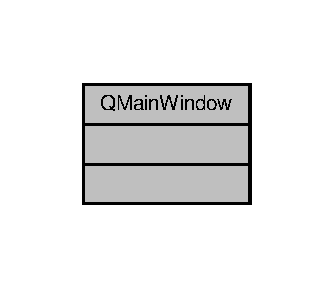
\includegraphics[width=160pt]{class_q_main_window__coll__graph}
\end{center}
\end{figure}


La documentation de cette classe a été générée à partir du fichier suivant \+:\begin{DoxyCompactItemize}
\item 
\hyperlink{_ihm_8h}{Ihm.\+h}\end{DoxyCompactItemize}

\hypertarget{class_q_object}{}\subsection{Référence de la classe Q\+Object}
\label{class_q_object}\index{Q\+Object@{Q\+Object}}


Graphe de collaboration de Q\+Object\+:
\nopagebreak
\begin{figure}[H]
\begin{center}
\leavevmode
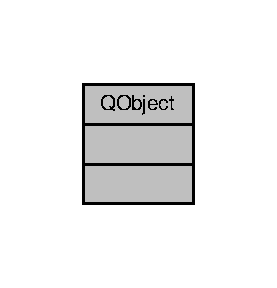
\includegraphics[width=133pt]{class_q_object__coll__graph}
\end{center}
\end{figure}


La documentation de cette classe a été générée à partir du fichier suivant \+:\begin{DoxyCompactItemize}
\item 
\hyperlink{_rfid_8h}{Rfid.\+h}\end{DoxyCompactItemize}

\hypertarget{class_q_push_button}{}\subsection{Référence de la classe Q\+Push\+Button}
\label{class_q_push_button}\index{Q\+Push\+Button@{Q\+Push\+Button}}


Graphe de collaboration de Q\+Push\+Button\+:
\nopagebreak
\begin{figure}[H]
\begin{center}
\leavevmode
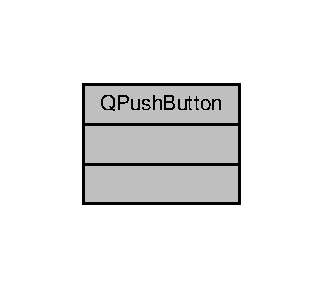
\includegraphics[width=155pt]{class_q_push_button__coll__graph}
\end{center}
\end{figure}


La documentation de cette classe a été générée à partir du fichier suivant \+:\begin{DoxyCompactItemize}
\item 
\hyperlink{_casier_8h}{Casier.\+h}\end{DoxyCompactItemize}

\hypertarget{class_rfid}{}\subsection{Référence de la classe Rfid}
\label{class_rfid}\index{Rfid@{Rfid}}


La classe \hyperlink{class_rfid}{Rfid} traite la trame reçue d\textquotesingle{}un lecteur \hyperlink{class_rfid}{Rfid}.  




{\ttfamily \#include $<$Rfid.\+h$>$}



Graphe de collaboration de Rfid\+:
\nopagebreak
\begin{figure}[H]
\begin{center}
\leavevmode
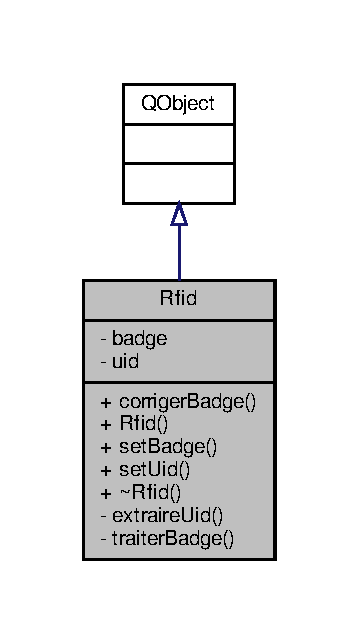
\includegraphics[width=172pt]{class_rfid__coll__graph}
\end{center}
\end{figure}
\subsubsection*{Signaux}
\begin{DoxyCompactItemize}
\item 
void \hyperlink{class_rfid_a896a20a2fbe2ac7d842456a1161717cb}{erreur\+Badge\+Invalide} (Q\+String message)
\item 
void \hyperlink{class_rfid_a76990ba3147098e80ac6fc67af6439d1}{nouveau\+Uid\+Badge} (Q\+String \hyperlink{class_rfid_ac634cd26ffbe1c6da3967dc4af53b734}{badge})
\end{DoxyCompactItemize}
\subsubsection*{Fonctions membres publiques}
\begin{DoxyCompactItemize}
\item 
Q\+String \hyperlink{class_rfid_afb99366646ac75b7e1d28302d38bf4f2}{corriger\+Badge} (Q\+String \hyperlink{class_rfid_ac634cd26ffbe1c6da3967dc4af53b734}{badge})
\begin{DoxyCompactList}\small\item\em Définition de la méthode \hyperlink{class_rfid_afb99366646ac75b7e1d28302d38bf4f2}{corriger\+Badge(\+Q\+String badge)} \end{DoxyCompactList}\item 
\hyperlink{class_rfid_aa00c7163ce0e3fda6596353d40a458a9}{Rfid} (\hyperlink{class_q_object}{Q\+Object} $\ast$parent=nullptr)
\begin{DoxyCompactList}\small\item\em Définition du constructeur de la classe \hyperlink{class_rfid}{Rfid}. \end{DoxyCompactList}\item 
void \hyperlink{class_rfid_a51021c0899dab1d5fb08e3dd6d93e425}{set\+Badge} (Q\+String \hyperlink{class_rfid_ac634cd26ffbe1c6da3967dc4af53b734}{badge})
\begin{DoxyCompactList}\small\item\em Définition de la méthode \hyperlink{class_rfid_a51021c0899dab1d5fb08e3dd6d93e425}{set\+Badge(\+Q\+String badge)} \end{DoxyCompactList}\item 
void \hyperlink{class_rfid_ac79b994b32bf7a7cbad9d9988e721564}{set\+Uid} (Q\+String \hyperlink{class_rfid_a157b71d282a7e067c65b431dbae6c6c8}{uid})
\begin{DoxyCompactList}\small\item\em Définition de la méthode \hyperlink{class_rfid_ac79b994b32bf7a7cbad9d9988e721564}{set\+Uid(\+Q\+String uid)} \end{DoxyCompactList}\item 
\hyperlink{class_rfid_a563836053a71a9fdc566a812da0cf5c1}{$\sim$\+Rfid} ()
\begin{DoxyCompactList}\small\item\em Définition du destructeur de la classe \hyperlink{class_rfid}{Rfid}. \end{DoxyCompactList}\end{DoxyCompactItemize}
\subsubsection*{Connecteurs privés}
\begin{DoxyCompactItemize}
\item 
void \hyperlink{class_rfid_a5b4f31b235afebee620e42c52ab60213}{traiter\+Badge} (Q\+String trame\+Badge)
\begin{DoxyCompactList}\small\item\em Définition de la méthode \hyperlink{class_rfid_a5b4f31b235afebee620e42c52ab60213}{Rfid\+::traiter\+Badge(\+Q\+String trame\+Badge)} \end{DoxyCompactList}\end{DoxyCompactItemize}
\subsubsection*{Fonctions membres privées}
\begin{DoxyCompactItemize}
\item 
void \hyperlink{class_rfid_a884e849f175045d78587e1e09a87cb00}{extraire\+Uid} ()
\begin{DoxyCompactList}\small\item\em Définition de la méthode \hyperlink{class_rfid_a884e849f175045d78587e1e09a87cb00}{Rfid\+::extraire\+Uid()} \end{DoxyCompactList}\end{DoxyCompactItemize}
\subsubsection*{Attributs privés}
\begin{DoxyCompactItemize}
\item 
Q\+String \hyperlink{class_rfid_ac634cd26ffbe1c6da3967dc4af53b734}{badge}
\begin{DoxyCompactList}\small\item\em trame reçue d\textquotesingle{}un badge \end{DoxyCompactList}\item 
Q\+String \hyperlink{class_rfid_a157b71d282a7e067c65b431dbae6c6c8}{uid}
\begin{DoxyCompactList}\small\item\em l\textquotesingle{}U\+ID extrait de la trame badge \end{DoxyCompactList}\end{DoxyCompactItemize}


\subsubsection{Description détaillée}
La classe \hyperlink{class_rfid}{Rfid} traite la trame reçue d\textquotesingle{}un lecteur \hyperlink{class_rfid}{Rfid}. 

\begin{DoxyAuthor}{Auteur}
Legger Pierre-\/\+Antoine
\end{DoxyAuthor}
\begin{DoxyVersion}{Version}
1.\+0
\end{DoxyVersion}
\begin{DoxyDate}{Date}
Mercredi 4 Mars 2020 
\end{DoxyDate}


Définition à la ligne \hyperlink{_rfid_8h_source_l00035}{35} du fichier \hyperlink{_rfid_8h_source}{Rfid.\+h}.



\subsubsection{Documentation des constructeurs et destructeur}
\mbox{\Hypertarget{class_rfid_aa00c7163ce0e3fda6596353d40a458a9}\label{class_rfid_aa00c7163ce0e3fda6596353d40a458a9}} 
\index{Rfid@{Rfid}!Rfid@{Rfid}}
\index{Rfid@{Rfid}!Rfid@{Rfid}}
\paragraph{\texorpdfstring{Rfid()}{Rfid()}}
{\footnotesize\ttfamily Rfid\+::\+Rfid (\begin{DoxyParamCaption}\item[{\hyperlink{class_q_object}{Q\+Object} $\ast$}]{parent = {\ttfamily nullptr} }\end{DoxyParamCaption})}



Définition du constructeur de la classe \hyperlink{class_rfid}{Rfid}. 

Initialise un objet \hyperlink{class_rfid}{Rfid} 
\begin{DoxyParams}{Paramètres}
{\em parent} & l\textquotesingle{}objet \hyperlink{class_q_object}{Q\+Object} parent \\
\hline
\end{DoxyParams}


Définition à la ligne \hyperlink{_rfid_8cpp_source_l00022}{22} du fichier \hyperlink{_rfid_8cpp_source}{Rfid.\+cpp}.


\begin{DoxyCode}
00022                           : \hyperlink{class_q_object}{QObject}(parent), \hyperlink{class_rfid_ac634cd26ffbe1c6da3967dc4af53b734}{badge}(\textcolor{stringliteral}{""})
00023 \{
00024 \}
\end{DoxyCode}
\mbox{\Hypertarget{class_rfid_a563836053a71a9fdc566a812da0cf5c1}\label{class_rfid_a563836053a71a9fdc566a812da0cf5c1}} 
\index{Rfid@{Rfid}!````~Rfid@{$\sim$\+Rfid}}
\index{````~Rfid@{$\sim$\+Rfid}!Rfid@{Rfid}}
\paragraph{\texorpdfstring{$\sim$\+Rfid()}{~Rfid()}}
{\footnotesize\ttfamily Rfid\+::$\sim$\+Rfid (\begin{DoxyParamCaption}{ }\end{DoxyParamCaption})}



Définition du destructeur de la classe \hyperlink{class_rfid}{Rfid}. 

Détruitun objet \hyperlink{class_rfid}{Rfid} 

Définition à la ligne \hyperlink{_rfid_8cpp_source_l00031}{31} du fichier \hyperlink{_rfid_8cpp_source}{Rfid.\+cpp}.


\begin{DoxyCode}
00032 \{
00033 
00034 \}
\end{DoxyCode}


\subsubsection{Documentation des fonctions membres}
\mbox{\Hypertarget{class_rfid_afb99366646ac75b7e1d28302d38bf4f2}\label{class_rfid_afb99366646ac75b7e1d28302d38bf4f2}} 
\index{Rfid@{Rfid}!corriger\+Badge@{corriger\+Badge}}
\index{corriger\+Badge@{corriger\+Badge}!Rfid@{Rfid}}
\paragraph{\texorpdfstring{corriger\+Badge()}{corrigerBadge()}}
{\footnotesize\ttfamily Q\+String Rfid\+::corriger\+Badge (\begin{DoxyParamCaption}\item[{Q\+String}]{badge }\end{DoxyParamCaption})}



Définition de la méthode \hyperlink{class_rfid_afb99366646ac75b7e1d28302d38bf4f2}{corriger\+Badge(\+Q\+String badge)} 

La trame reçue provient de l\textquotesingle{}émulation d\textquotesingle{}un clavier Q\+W\+E\+R\+TY qu\textquotesingle{}il faut traduire en A\+Z\+E\+R\+TY 
\begin{DoxyParams}{Paramètres}
{\em badge} & la trame badge en format Q\+W\+E\+R\+TY \\
\hline
\end{DoxyParams}
\begin{DoxyReturn}{Renvoie}
la trame badge en format A\+Z\+E\+R\+TY 
\end{DoxyReturn}


Définition à la ligne \hyperlink{_rfid_8cpp_source_l00043}{43} du fichier \hyperlink{_rfid_8cpp_source}{Rfid.\+cpp}.



Référencé par \hyperlink{_rfid_8cpp_source_l00097}{traiter\+Badge()}.


\begin{DoxyCode}
00044 \{
00045     QString badgeCorrige = \textcolor{stringliteral}{""};
00046 
00047     \textcolor{keywordflow}{if}(!\hyperlink{class_rfid_ac634cd26ffbe1c6da3967dc4af53b734}{badge}.isEmpty())
00048     \{
00049         \textcolor{comment}{// effectue les remplacements des touches QWERTY en touches AZERTY}
00050         badgeCorrige = \hyperlink{class_rfid_ac634cd26ffbe1c6da3967dc4af53b734}{badge}.replace(QString::fromUtf8(\textcolor{stringliteral}{"Q"}), \textcolor{stringliteral}{"A"});
00051         badgeCorrige = \hyperlink{class_rfid_ac634cd26ffbe1c6da3967dc4af53b734}{badge}.replace(QString::fromUtf8(\textcolor{stringliteral}{"W"}), \textcolor{stringliteral}{"Z"});
00052         badgeCorrige = \hyperlink{class_rfid_ac634cd26ffbe1c6da3967dc4af53b734}{badge}.replace(QString::fromUtf8(\textcolor{stringliteral}{"q"}), \textcolor{stringliteral}{"q"});
00053         badgeCorrige = \hyperlink{class_rfid_ac634cd26ffbe1c6da3967dc4af53b734}{badge}.replace(QString::fromUtf8(\textcolor{stringliteral}{"w"}), \textcolor{stringliteral}{"z"});
00054         badgeCorrige = \hyperlink{class_rfid_ac634cd26ffbe1c6da3967dc4af53b734}{badge}.replace(QString::fromUtf8(\textcolor{stringliteral}{"M"}), \textcolor{stringliteral}{":"});
00055         badgeCorrige = \hyperlink{class_rfid_ac634cd26ffbe1c6da3967dc4af53b734}{badge}.replace(QString::fromUtf8(\textcolor{stringliteral}{"à"}), \textcolor{stringliteral}{"0"});
00056         badgeCorrige = \hyperlink{class_rfid_ac634cd26ffbe1c6da3967dc4af53b734}{badge}.replace(QString::fromUtf8(\textcolor{stringliteral}{"&"}), \textcolor{stringliteral}{"1"});
00057         badgeCorrige = \hyperlink{class_rfid_ac634cd26ffbe1c6da3967dc4af53b734}{badge}.replace(QString::fromUtf8(\textcolor{stringliteral}{"é"}), \textcolor{stringliteral}{"2"});
00058         badgeCorrige = \hyperlink{class_rfid_ac634cd26ffbe1c6da3967dc4af53b734}{badge}.replace(QString::fromUtf8(\textcolor{stringliteral}{"\(\backslash\)""}), \textcolor{stringliteral}{"3"});
00059         badgeCorrige = \hyperlink{class_rfid_ac634cd26ffbe1c6da3967dc4af53b734}{badge}.replace(QString::fromUtf8(\textcolor{stringliteral}{"'"}), \textcolor{stringliteral}{"4"});
00060         badgeCorrige = \hyperlink{class_rfid_ac634cd26ffbe1c6da3967dc4af53b734}{badge}.replace(QString::fromUtf8(\textcolor{stringliteral}{"("}), \textcolor{stringliteral}{"5"});
00061         badgeCorrige = \hyperlink{class_rfid_ac634cd26ffbe1c6da3967dc4af53b734}{badge}.replace(QString::fromUtf8(\textcolor{stringliteral}{"-"}), \textcolor{stringliteral}{"6"});
00062         badgeCorrige = \hyperlink{class_rfid_ac634cd26ffbe1c6da3967dc4af53b734}{badge}.replace(QString::fromUtf8(\textcolor{stringliteral}{"è"}), \textcolor{stringliteral}{"7"});
00063         badgeCorrige = \hyperlink{class_rfid_ac634cd26ffbe1c6da3967dc4af53b734}{badge}.replace(QString::fromUtf8(\textcolor{stringliteral}{"\_"}), \textcolor{stringliteral}{"8"});
00064         badgeCorrige = \hyperlink{class_rfid_ac634cd26ffbe1c6da3967dc4af53b734}{badge}.replace(QString::fromUtf8(\textcolor{stringliteral}{"ç"}), \textcolor{stringliteral}{"9"});
00065     \}
00066     \textcolor{keywordflow}{return} badgeCorrige;
00067 \}
\end{DoxyCode}
\mbox{\Hypertarget{class_rfid_a896a20a2fbe2ac7d842456a1161717cb}\label{class_rfid_a896a20a2fbe2ac7d842456a1161717cb}} 
\index{Rfid@{Rfid}!erreur\+Badge\+Invalide@{erreur\+Badge\+Invalide}}
\index{erreur\+Badge\+Invalide@{erreur\+Badge\+Invalide}!Rfid@{Rfid}}
\paragraph{\texorpdfstring{erreur\+Badge\+Invalide}{erreurBadgeInvalide}}
{\footnotesize\ttfamily void Rfid\+::erreur\+Badge\+Invalide (\begin{DoxyParamCaption}\item[{Q\+String}]{message }\end{DoxyParamCaption})\hspace{0.3cm}{\ttfamily [signal]}}



Référencé par \hyperlink{_rfid_8cpp_source_l00097}{traiter\+Badge()}.

\mbox{\Hypertarget{class_rfid_a884e849f175045d78587e1e09a87cb00}\label{class_rfid_a884e849f175045d78587e1e09a87cb00}} 
\index{Rfid@{Rfid}!extraire\+Uid@{extraire\+Uid}}
\index{extraire\+Uid@{extraire\+Uid}!Rfid@{Rfid}}
\paragraph{\texorpdfstring{extraire\+Uid()}{extraireUid()}}
{\footnotesize\ttfamily void Rfid\+::extraire\+Uid (\begin{DoxyParamCaption}{ }\end{DoxyParamCaption})\hspace{0.3cm}{\ttfamily [private]}}



Définition de la méthode \hyperlink{class_rfid_a884e849f175045d78587e1e09a87cb00}{Rfid\+::extraire\+Uid()} 

Extrait l\textquotesingle{}U\+ID de la trame badge 

Définition à la ligne \hyperlink{_rfid_8cpp_source_l00130}{130} du fichier \hyperlink{_rfid_8cpp_source}{Rfid.\+cpp}.



Références \hyperlink{_rfid_8h_source_l00056}{badge}, et \hyperlink{_rfid_8cpp_source_l00086}{set\+Uid()}.



Référencé par \hyperlink{_rfid_8cpp_source_l00097}{traiter\+Badge()}.


\begin{DoxyCode}
00131 \{
00132     \hyperlink{class_rfid_ac79b994b32bf7a7cbad9d9988e721564}{setUid}(\hyperlink{class_rfid_ac634cd26ffbe1c6da3967dc4af53b734}{badge}.section(\textcolor{charliteral}{':'},1,1));
00133 \}
\end{DoxyCode}
\mbox{\Hypertarget{class_rfid_a76990ba3147098e80ac6fc67af6439d1}\label{class_rfid_a76990ba3147098e80ac6fc67af6439d1}} 
\index{Rfid@{Rfid}!nouveau\+Uid\+Badge@{nouveau\+Uid\+Badge}}
\index{nouveau\+Uid\+Badge@{nouveau\+Uid\+Badge}!Rfid@{Rfid}}
\paragraph{\texorpdfstring{nouveau\+Uid\+Badge}{nouveauUidBadge}}
{\footnotesize\ttfamily void Rfid\+::nouveau\+Uid\+Badge (\begin{DoxyParamCaption}\item[{Q\+String}]{badge }\end{DoxyParamCaption})\hspace{0.3cm}{\ttfamily [signal]}}



Référencé par \hyperlink{_rfid_8cpp_source_l00097}{traiter\+Badge()}.

\mbox{\Hypertarget{class_rfid_a51021c0899dab1d5fb08e3dd6d93e425}\label{class_rfid_a51021c0899dab1d5fb08e3dd6d93e425}} 
\index{Rfid@{Rfid}!set\+Badge@{set\+Badge}}
\index{set\+Badge@{set\+Badge}!Rfid@{Rfid}}
\paragraph{\texorpdfstring{set\+Badge()}{setBadge()}}
{\footnotesize\ttfamily void Rfid\+::set\+Badge (\begin{DoxyParamCaption}\item[{Q\+String}]{badge }\end{DoxyParamCaption})}



Définition de la méthode \hyperlink{class_rfid_a51021c0899dab1d5fb08e3dd6d93e425}{set\+Badge(\+Q\+String badge)} 

Accesseur set de l\textquotesingle{}attribut badge 
\begin{DoxyParams}{Paramètres}
{\em badge} & \\
\hline
\end{DoxyParams}


Définition à la ligne \hyperlink{_rfid_8cpp_source_l00075}{75} du fichier \hyperlink{_rfid_8cpp_source}{Rfid.\+cpp}.



Références \hyperlink{_rfid_8h_source_l00056}{badge}.



Référencé par \hyperlink{_rfid_8cpp_source_l00097}{traiter\+Badge()}.


\begin{DoxyCode}
00076 \{
00077     this->\hyperlink{class_rfid_ac634cd26ffbe1c6da3967dc4af53b734}{badge} = \hyperlink{class_rfid_ac634cd26ffbe1c6da3967dc4af53b734}{badge};
00078 \}
\end{DoxyCode}
\mbox{\Hypertarget{class_rfid_ac79b994b32bf7a7cbad9d9988e721564}\label{class_rfid_ac79b994b32bf7a7cbad9d9988e721564}} 
\index{Rfid@{Rfid}!set\+Uid@{set\+Uid}}
\index{set\+Uid@{set\+Uid}!Rfid@{Rfid}}
\paragraph{\texorpdfstring{set\+Uid()}{setUid()}}
{\footnotesize\ttfamily void Rfid\+::set\+Uid (\begin{DoxyParamCaption}\item[{Q\+String}]{uid }\end{DoxyParamCaption})}



Définition de la méthode \hyperlink{class_rfid_ac79b994b32bf7a7cbad9d9988e721564}{set\+Uid(\+Q\+String uid)} 

Accesseur set de l\textquotesingle{}attribut uid 
\begin{DoxyParams}{Paramètres}
{\em uid} & \\
\hline
\end{DoxyParams}


Définition à la ligne \hyperlink{_rfid_8cpp_source_l00086}{86} du fichier \hyperlink{_rfid_8cpp_source}{Rfid.\+cpp}.



Références \hyperlink{_rfid_8h_source_l00057}{uid}.



Référencé par \hyperlink{_rfid_8cpp_source_l00130}{extraire\+Uid()}.


\begin{DoxyCode}
00087 \{
00088     this->\hyperlink{class_rfid_a157b71d282a7e067c65b431dbae6c6c8}{uid} = \hyperlink{class_rfid_a157b71d282a7e067c65b431dbae6c6c8}{uid};
00089 \}
\end{DoxyCode}
\mbox{\Hypertarget{class_rfid_a5b4f31b235afebee620e42c52ab60213}\label{class_rfid_a5b4f31b235afebee620e42c52ab60213}} 
\index{Rfid@{Rfid}!traiter\+Badge@{traiter\+Badge}}
\index{traiter\+Badge@{traiter\+Badge}!Rfid@{Rfid}}
\paragraph{\texorpdfstring{traiter\+Badge}{traiterBadge}}
{\footnotesize\ttfamily void Rfid\+::traiter\+Badge (\begin{DoxyParamCaption}\item[{Q\+String}]{trame\+Badge }\end{DoxyParamCaption})\hspace{0.3cm}{\ttfamily [private]}, {\ttfamily [slot]}}



Définition de la méthode \hyperlink{class_rfid_a5b4f31b235afebee620e42c52ab60213}{Rfid\+::traiter\+Badge(\+Q\+String trame\+Badge)} 

Extrait l\textquotesingle{}U\+ID d\textquotesingle{}une trame badge valide 
\begin{DoxyParams}{Paramètres}
{\em trame\+Badge} & la trame reçue du lecteur \hyperlink{class_rfid}{Rfid} \\
\hline
\end{DoxyParams}


Définition à la ligne \hyperlink{_rfid_8cpp_source_l00097}{97} du fichier \hyperlink{_rfid_8cpp_source}{Rfid.\+cpp}.



Références \hyperlink{_rfid_8h_source_l00056}{badge}, \hyperlink{_rfid_8cpp_source_l00043}{corriger\+Badge()}, \hyperlink{_rfid_8h_source_l00018}{E\+R\+R\+E\+U\+R\+\_\+\+B\+A\+D\+G\+E\+\_\+\+I\+N\+V\+A\+L\+I\+DE}, \hyperlink{class_rfid_a896a20a2fbe2ac7d842456a1161717cb}{erreur\+Badge\+Invalide()}, \hyperlink{_rfid_8cpp_source_l00130}{extraire\+Uid()}, \hyperlink{class_rfid_a76990ba3147098e80ac6fc67af6439d1}{nouveau\+Uid\+Badge()}, \hyperlink{_rfid_8cpp_source_l00075}{set\+Badge()}, et \hyperlink{_rfid_8h_source_l00057}{uid}.


\begin{DoxyCode}
00098 \{
00099     \textcolor{comment}{/*}
00100 \textcolor{comment}{     * Format trame reçue : RFID:xxxxxxxx}
00101 \textcolor{comment}{     * xxxxxxxx -> uid du badge}
00102 \textcolor{comment}{     */}
00103     \hyperlink{class_rfid_a51021c0899dab1d5fb08e3dd6d93e425}{setBadge}(\hyperlink{class_rfid_afb99366646ac75b7e1d28302d38bf4f2}{corrigerBadge}(trameBadge));    
00104 
00105 \textcolor{preprocessor}{    #ifdef DEBUG\_RFID}
00106         qDebug() << Q\_FUNC\_INFO << \textcolor{stringliteral}{"Badge"} << \hyperlink{class_rfid_ac634cd26ffbe1c6da3967dc4af53b734}{badge};
00107 \textcolor{preprocessor}{    #endif}
00108 
00109     \textcolor{comment}{// Vérifier si la trame est valide}
00110     \textcolor{keywordflow}{if}(badge.startsWith(\textcolor{stringliteral}{"RFID:"}))
00111     \{
00112         \hyperlink{class_rfid_a884e849f175045d78587e1e09a87cb00}{extraireUid}();
00113 
00114         emit \hyperlink{class_rfid_a76990ba3147098e80ac6fc67af6439d1}{nouveauUidBadge}(\hyperlink{class_rfid_a157b71d282a7e067c65b431dbae6c6c8}{uid});
00115 \textcolor{preprocessor}{        #ifdef DEBUG\_RFID}
00116             qDebug() << Q\_FUNC\_INFO << \textcolor{stringliteral}{"UID"} << \hyperlink{class_rfid_a157b71d282a7e067c65b431dbae6c6c8}{uid};
00117 \textcolor{preprocessor}{        #endif}
00118     \}
00119     \textcolor{keywordflow}{else}
00120     \{
00121         emit \hyperlink{class_rfid_a896a20a2fbe2ac7d842456a1161717cb}{erreurBadgeInvalide}(\hyperlink{_rfid_8h_aad43c23a448ffc828e0b6014cfaf980a}{ERREUR\_BADGE\_INVALIDE});
00122     \}
00123 \}
\end{DoxyCode}


\subsubsection{Documentation des données membres}
\mbox{\Hypertarget{class_rfid_ac634cd26ffbe1c6da3967dc4af53b734}\label{class_rfid_ac634cd26ffbe1c6da3967dc4af53b734}} 
\index{Rfid@{Rfid}!badge@{badge}}
\index{badge@{badge}!Rfid@{Rfid}}
\paragraph{\texorpdfstring{badge}{badge}}
{\footnotesize\ttfamily Q\+String Rfid\+::badge\hspace{0.3cm}{\ttfamily [private]}}



trame reçue d\textquotesingle{}un badge 



Définition à la ligne \hyperlink{_rfid_8h_source_l00056}{56} du fichier \hyperlink{_rfid_8h_source}{Rfid.\+h}.



Référencé par \hyperlink{_rfid_8cpp_source_l00130}{extraire\+Uid()}, \hyperlink{_rfid_8cpp_source_l00075}{set\+Badge()}, et \hyperlink{_rfid_8cpp_source_l00097}{traiter\+Badge()}.

\mbox{\Hypertarget{class_rfid_a157b71d282a7e067c65b431dbae6c6c8}\label{class_rfid_a157b71d282a7e067c65b431dbae6c6c8}} 
\index{Rfid@{Rfid}!uid@{uid}}
\index{uid@{uid}!Rfid@{Rfid}}
\paragraph{\texorpdfstring{uid}{uid}}
{\footnotesize\ttfamily Q\+String Rfid\+::uid\hspace{0.3cm}{\ttfamily [private]}}



l\textquotesingle{}U\+ID extrait de la trame badge 



Définition à la ligne \hyperlink{_rfid_8h_source_l00057}{57} du fichier \hyperlink{_rfid_8h_source}{Rfid.\+h}.



Référencé par \hyperlink{_rfid_8cpp_source_l00086}{set\+Uid()}, et \hyperlink{_rfid_8cpp_source_l00097}{traiter\+Badge()}.



La documentation de cette classe a été générée à partir des fichiers suivants \+:\begin{DoxyCompactItemize}
\item 
\hyperlink{_rfid_8h}{Rfid.\+h}\item 
\hyperlink{_rfid_8cpp}{Rfid.\+cpp}\end{DoxyCompactItemize}

\hypertarget{class_supervision}{}\subsection{Référence de la classe Supervision}
\label{class_supervision}\index{Supervision@{Supervision}}


La classe \hyperlink{class_supervision}{Supervision} permet de superviser l\textquotesingle{}ensemble de l\textquotesingle{}application.  




{\ttfamily \#include $<$Supervision.\+h$>$}



Graphe de collaboration de Supervision\+:
\nopagebreak
\begin{figure}[H]
\begin{center}
\leavevmode
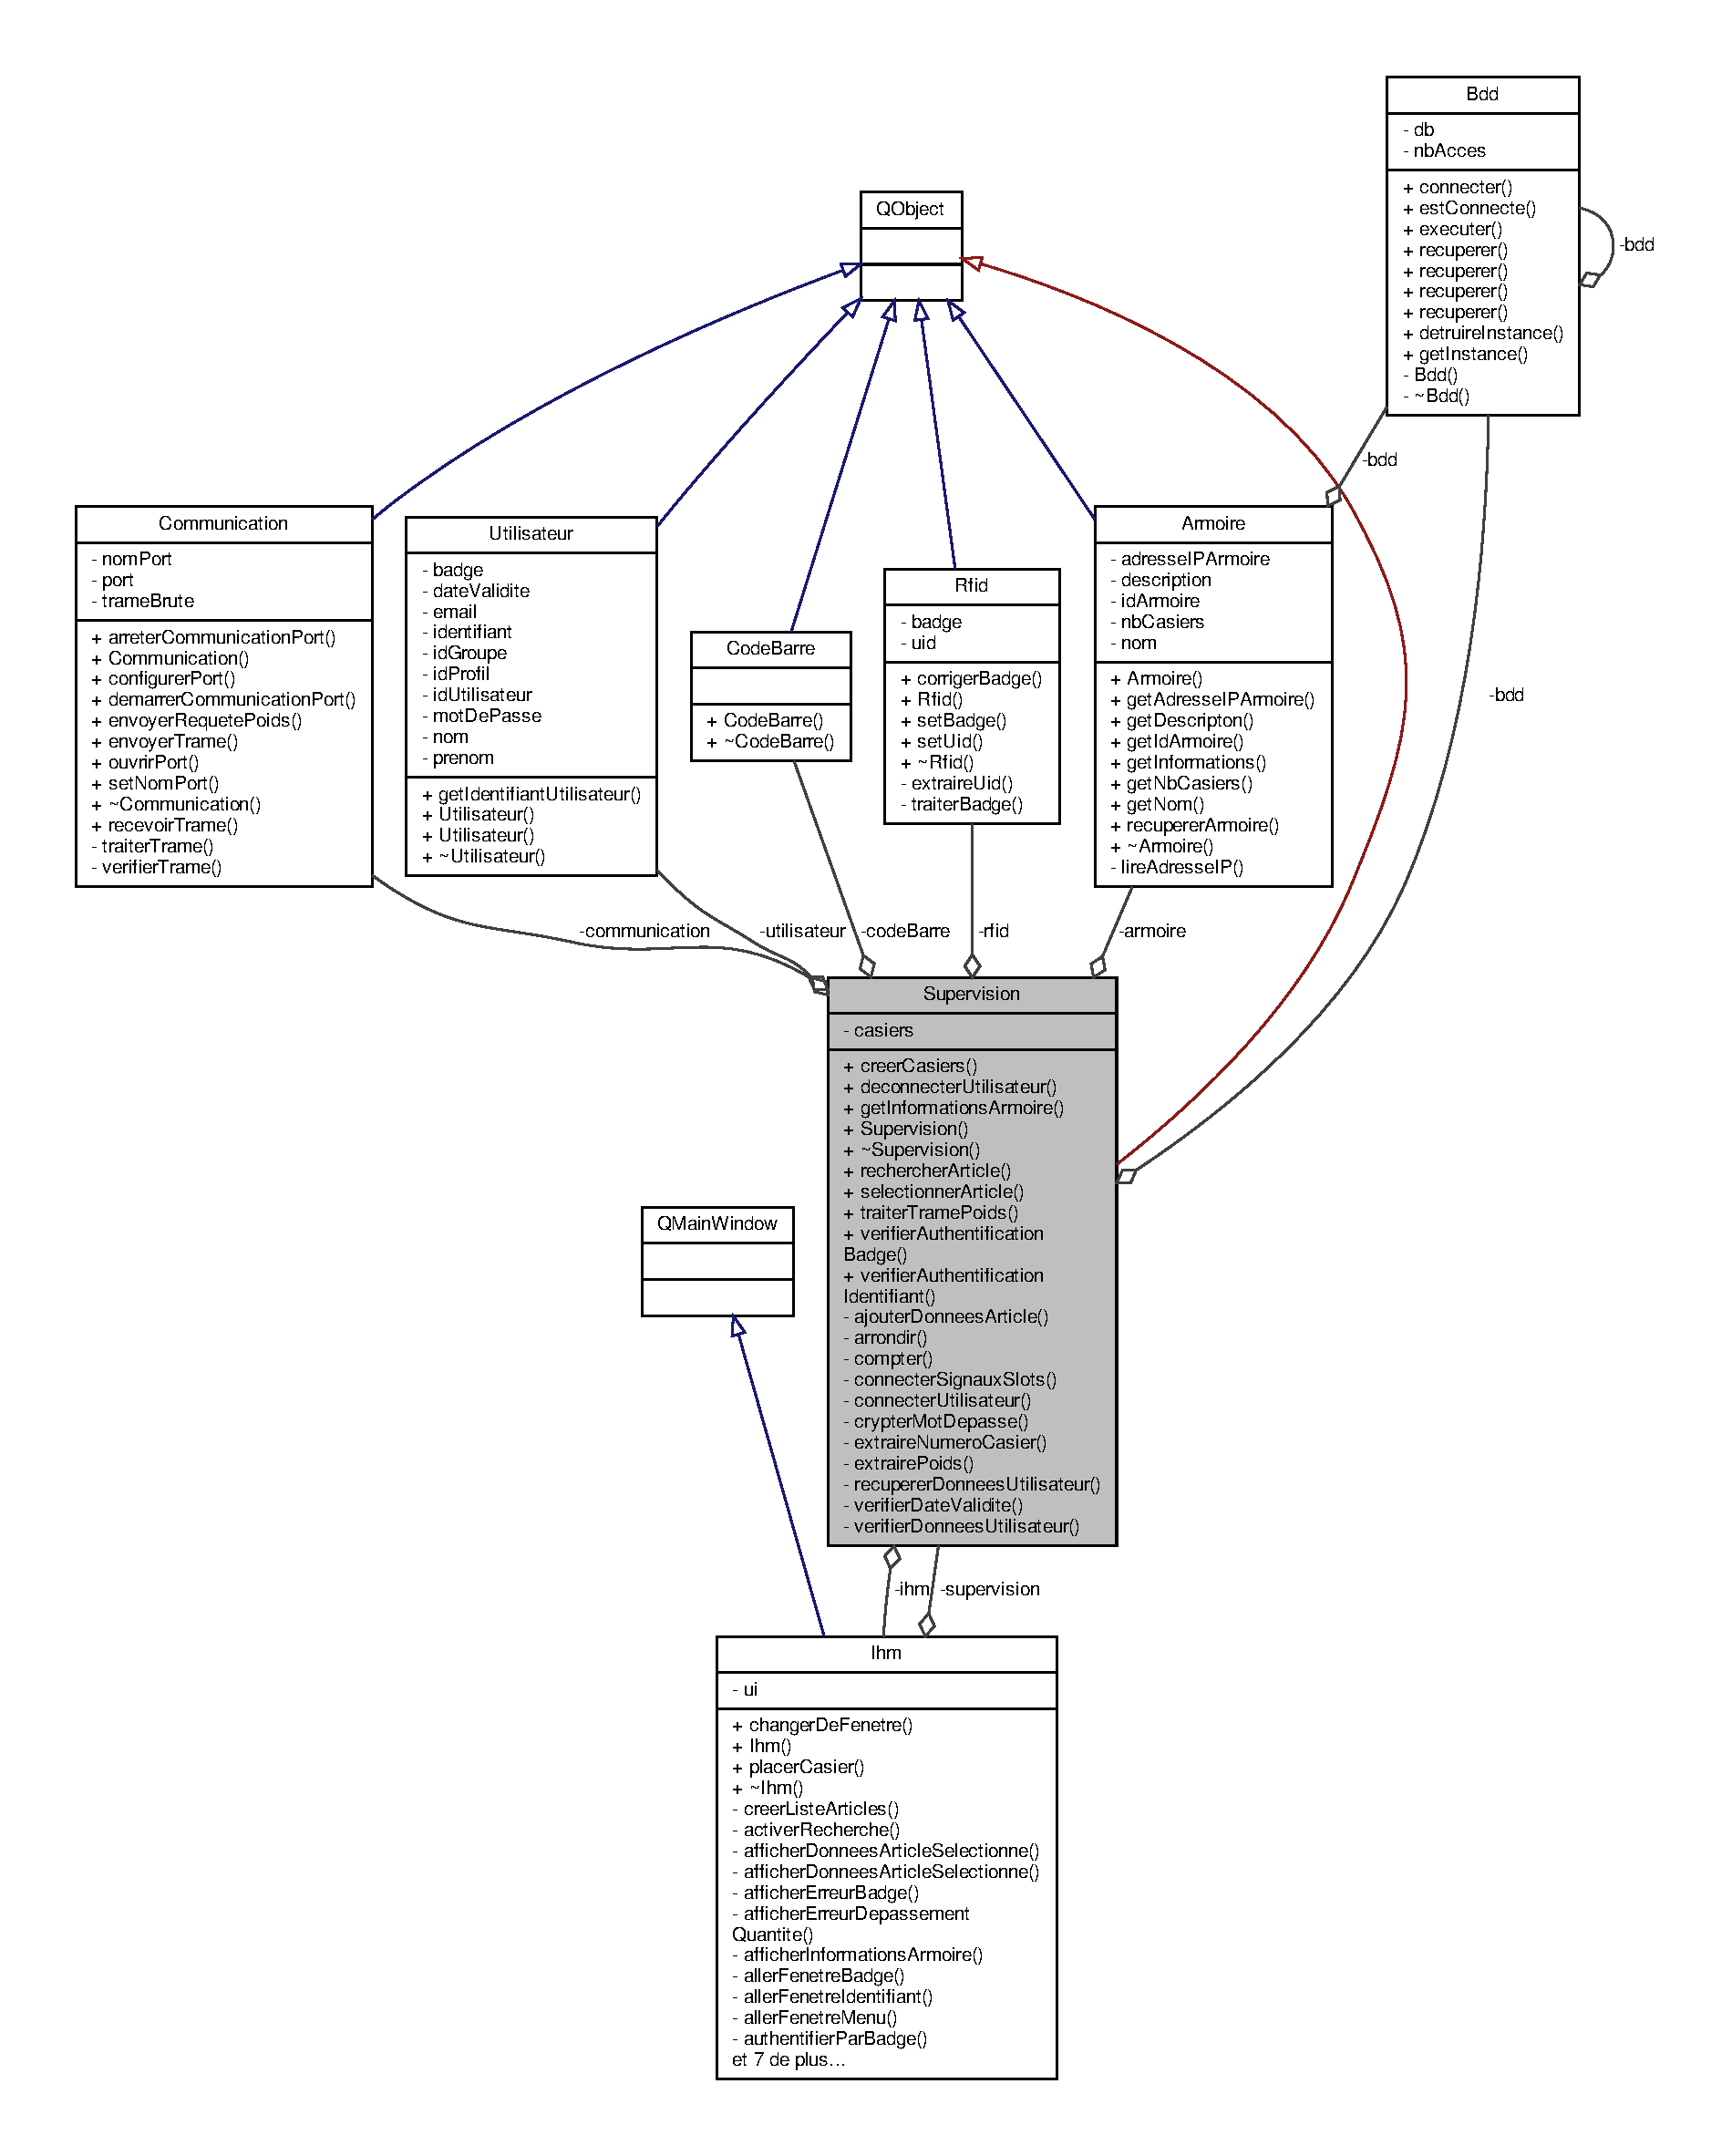
\includegraphics[width=350pt]{class_supervision__coll__graph}
\end{center}
\end{figure}
\subsubsection*{Connecteurs publics}
\begin{DoxyCompactItemize}
\item 
void \hyperlink{class_supervision_af2df200be6727338110b81812703d0ae}{rechercher\+Article} (Q\+String recherche)
\begin{DoxyCompactList}\small\item\em Définition de la méthode rechercher\+Article. \end{DoxyCompactList}\item 
void \hyperlink{class_supervision_a2efb7e4dabe2664c9cfd41d703b6250c}{selectionner\+Article} (Q\+String nom\+Article)
\begin{DoxyCompactList}\small\item\em Définition de la méthode selectionner\+Article. \end{DoxyCompactList}\item 
void \hyperlink{class_supervision_ae72bdcb7d70bbb8e13cf61be95ee7c06}{traiter\+Trame\+Poids} (Q\+String trame)
\begin{DoxyCompactList}\small\item\em Définition de la méthode traiter\+Trame\+Poids. \end{DoxyCompactList}\item 
void \hyperlink{class_supervision_a07e7f0cd8b114182be56ebb5645e62fe}{verifier\+Authentification\+Badge} (Q\+String badge)
\begin{DoxyCompactList}\small\item\em Définition de la méthode verifier\+Authentification\+Badge. \end{DoxyCompactList}\item 
void \hyperlink{class_supervision_ac596674d302f1f747d65c8334aa1ced9}{verifier\+Authentification\+Identifiant} (Q\+String identifiant, Q\+String mot\+De\+Passe)
\begin{DoxyCompactList}\small\item\em Définition de la méthode verifier\+Authentification\+Identifiant. \end{DoxyCompactList}\end{DoxyCompactItemize}
\subsubsection*{Signaux}
\begin{DoxyCompactItemize}
\item 
void \hyperlink{class_supervision_a3023468d106abfe7dc697e61a63778ed}{articles\+Trouves} (Q\+Vector$<$ Q\+String\+List $>$)
\item 
void \hyperlink{class_supervision_ae486eafc331964e223c35ae2b54fa669}{donnees\+Article\+Selectionne} (Q\+Vector$<$ Q\+String\+List $>$)
\item 
void \hyperlink{class_supervision_ae01e53be90edf2656432c5da56331b9d}{donnees\+Article\+Selectionne} (Q\+String\+List)
\item 
void \hyperlink{class_supervision_a3fb19a3c16324a21af956fd272ca469d}{erreur\+Depassement\+Quantite} ()
\item 
void \hyperlink{class_supervision_a116ed6de0e9e3c9c94886235e9f6d6e8}{reponse\+Demande\+De\+Connexion} (bool, Q\+String)
\end{DoxyCompactItemize}
\subsubsection*{Fonctions membres publiques}
\begin{DoxyCompactItemize}
\item 
void \hyperlink{class_supervision_a558665fd7e7c44653907883afd9a58bf}{creer\+Casiers} ()
\begin{DoxyCompactList}\small\item\em Définition de la méthode creer\+Casiers. \end{DoxyCompactList}\item 
void \hyperlink{class_supervision_a164a1ad89264ea252401818df325eab8}{deconnecter\+Utilisateur} ()
\begin{DoxyCompactList}\small\item\em Méthode qui permet la déconnexion de l\textquotesingle{}utilisateur. \end{DoxyCompactList}\item 
Q\+String\+List \hyperlink{class_supervision_a72bd93799fcf5423a5f0c5538d4ec892}{get\+Informations\+Armoire} ()
\begin{DoxyCompactList}\small\item\em Définition de la méthode get\+Informations\+Armoire. \end{DoxyCompactList}\item 
\hyperlink{class_supervision_af3f0ed8f5aadd6b4aa5e0eac2813d8c4}{Supervision} (\hyperlink{class_ihm}{Ihm} $\ast$parent=nullptr)
\begin{DoxyCompactList}\small\item\em Définition du constructeur de la classe \hyperlink{class_supervision}{Supervision}. \end{DoxyCompactList}\item 
\hyperlink{class_supervision_a5058e6aec3356006c8efe66bf223ec94}{$\sim$\+Supervision} ()
\begin{DoxyCompactList}\small\item\em Définition du destructeur de \hyperlink{class_supervision}{Supervision}. \end{DoxyCompactList}\end{DoxyCompactItemize}
\subsubsection*{Fonctions membres privées}
\begin{DoxyCompactItemize}
\item 
void \hyperlink{class_supervision_ae6fc43cb8bdfd8045367c08d8e440359}{ajouter\+Donnees\+Article} (\hyperlink{class_article}{Article} $\ast$article, Q\+Vector$<$ Q\+String\+List $>$ \&donnees\+Article, Q\+String\+List \&donnees)
\begin{DoxyCompactList}\small\item\em Définition de la méthode ajouter\+Donnees\+Article. \end{DoxyCompactList}\item 
int \hyperlink{class_supervision_a16fde33340a8bc8b0936926cd6dc0657}{arrondir} (Q\+String arrondire)
\begin{DoxyCompactList}\small\item\em Définition de la méthode arrondir. \end{DoxyCompactList}\item 
int \hyperlink{class_supervision_a81b1b8960cb2857be4a6789cf27cd413}{compter} (Q\+String poid\+Article, Q\+String poid\+Total, Q\+String tare)
\begin{DoxyCompactList}\small\item\em Définition de la méthode compter. \end{DoxyCompactList}\item 
void \hyperlink{class_supervision_ac3bb2f3834b09a81ae9a767502ff693b}{connecter\+Signaux\+Slots} ()
\begin{DoxyCompactList}\small\item\em Définition de la méthode connecter\+Signaux\+Slots. \end{DoxyCompactList}\item 
void \hyperlink{class_supervision_a7c397ca5f79afa2709a657d7185dfbe1}{connecter\+Utilisateur} (Q\+String\+List \&donnees)
\begin{DoxyCompactList}\small\item\em Définition de la méthode connecter\+Utilisateur. \end{DoxyCompactList}\item 
void \hyperlink{class_supervision_ac58c5b922ce85af75c2233cd3265d201}{crypter\+Mot\+Depasse} (Q\+String \&mot\+De\+Passe)
\begin{DoxyCompactList}\small\item\em Définition de la méthode crypter\+Mot\+Depasse. \end{DoxyCompactList}\item 
Q\+String \hyperlink{class_supervision_a141a35024b0cb74636a8c6810a1ab26d}{extraire\+Numero\+Casier} (Q\+String trame)
\begin{DoxyCompactList}\small\item\em Définition de la méthode extraire\+Numero\+Casier. \end{DoxyCompactList}\item 
Q\+String \hyperlink{class_supervision_afdef41cd85f2ecfae9d1dc46f556a034}{extraire\+Poids} (Q\+String trame)
\begin{DoxyCompactList}\small\item\em Définition de la méthode extraire\+Poids. \end{DoxyCompactList}\item 
Q\+String\+List \hyperlink{class_supervision_a137b6c505742a4ada6ab38193eef01dd}{recuperer\+Donnees\+Utilisateur} (Q\+String requete\+B\+DD)
\begin{DoxyCompactList}\small\item\em Définition de la méthode recuperer\+Donnees\+Utilisateur. \end{DoxyCompactList}\item 
bool \hyperlink{class_supervision_acc886b933823993f1e3873582e05e690}{verifier\+Date\+Validite} (Q\+String string\+Date\+Validite)
\begin{DoxyCompactList}\small\item\em Définition de la méthode verifier\+Date\+Validite. \end{DoxyCompactList}\item 
bool \hyperlink{class_supervision_ae3400dad53c52bc09198e8d7f80e0e67}{verifier\+Donnees\+Utilisateur} (Q\+String\+List \&donnees)
\begin{DoxyCompactList}\small\item\em Définition de la méthode verifier\+Donnees\+Utilisateur. \end{DoxyCompactList}\end{DoxyCompactItemize}
\subsubsection*{Attributs privés}
\begin{DoxyCompactItemize}
\item 
\hyperlink{class_armoire}{Armoire} $\ast$ \hyperlink{class_supervision_a9f974b5c47899192395e539a0f11034c}{armoire}
\begin{DoxyCompactList}\small\item\em association d\textquotesingle{}un objet \hyperlink{class_armoire}{Armoire} \end{DoxyCompactList}\item 
\hyperlink{class_bdd}{Bdd} $\ast$ \hyperlink{class_supervision_ac9a970d4f511f2eed5da4aed037533ab}{bdd}
\begin{DoxyCompactList}\small\item\em association d\textquotesingle{}un objet \hyperlink{class_bdd}{Bdd} (accès à la base de données) \end{DoxyCompactList}\item 
Q\+Vector$<$ \hyperlink{class_casier}{Casier} $\ast$ $>$ \hyperlink{class_supervision_a3ac996538c83f3bd3df36095b0abb1b2}{casiers}
\begin{DoxyCompactList}\small\item\em les casiers de l\textquotesingle{}armoire \end{DoxyCompactList}\item 
\hyperlink{class_code_barre}{Code\+Barre} $\ast$ \hyperlink{class_supervision_ac01c57f7fd9d043ab46d439e55e426e5}{code\+Barre}
\begin{DoxyCompactList}\small\item\em association d\textquotesingle{}un objet \hyperlink{class_code_barre}{Code\+Barre} \end{DoxyCompactList}\item 
\hyperlink{class_communication}{Communication} $\ast$ \hyperlink{class_supervision_a045be64d74de4f7688574eec108220a5}{communication}
\begin{DoxyCompactList}\small\item\em association d\textquotesingle{}un objet \hyperlink{class_communication}{Communication} \end{DoxyCompactList}\item 
\hyperlink{class_ihm}{Ihm} $\ast$ \hyperlink{class_supervision_a5aa823c55bf1531497bbb8fdbc6c5528}{ihm}
\begin{DoxyCompactList}\small\item\em association d\textquotesingle{}un objet \hyperlink{class_ihm}{Ihm} (fenêtre princiaple de l\textquotesingle{}application) \end{DoxyCompactList}\item 
\hyperlink{class_rfid}{Rfid} $\ast$ \hyperlink{class_supervision_a3ec5986105208e9a2b02b7e97bf61090}{rfid}
\begin{DoxyCompactList}\small\item\em association d\textquotesingle{}un objet \hyperlink{class_rfid}{Rfid} (le lecteur de badge) \end{DoxyCompactList}\item 
\hyperlink{class_utilisateur}{Utilisateur} $\ast$ \hyperlink{class_supervision_a92384f2b12b2549cee988f83add8ad49}{utilisateur}
\begin{DoxyCompactList}\small\item\em association d\textquotesingle{}un objet \hyperlink{class_utilisateur}{Utilisateur} (l\textquotesingle{}utilisateur authentifié) \end{DoxyCompactList}\end{DoxyCompactItemize}


\subsubsection{Description détaillée}
La classe \hyperlink{class_supervision}{Supervision} permet de superviser l\textquotesingle{}ensemble de l\textquotesingle{}application. 

\begin{DoxyAuthor}{Auteur}
Legger Pierre-\/\+Antoine 

Tranchat Joffrey
\end{DoxyAuthor}
\begin{DoxyVersion}{Version}
1.\+0
\end{DoxyVersion}
\begin{DoxyDate}{Date}
Mercredi 12 Février 2020 
\end{DoxyDate}


Définition à la ligne \hyperlink{_supervision_8h_source_l00052}{52} du fichier \hyperlink{_supervision_8h_source}{Supervision.\+h}.



\subsubsection{Documentation des constructeurs et destructeur}
\mbox{\Hypertarget{class_supervision_af3f0ed8f5aadd6b4aa5e0eac2813d8c4}\label{class_supervision_af3f0ed8f5aadd6b4aa5e0eac2813d8c4}} 
\index{Supervision@{Supervision}!Supervision@{Supervision}}
\index{Supervision@{Supervision}!Supervision@{Supervision}}
\paragraph{\texorpdfstring{Supervision()}{Supervision()}}
{\footnotesize\ttfamily Supervision\+::\+Supervision (\begin{DoxyParamCaption}\item[{\hyperlink{class_ihm}{Ihm} $\ast$}]{parent = {\ttfamily nullptr} }\end{DoxyParamCaption})}



Définition du constructeur de la classe \hyperlink{class_supervision}{Supervision}. 

Initialise la supervision 
\begin{DoxyParams}{Paramètres}
{\em parent} & l\textquotesingle{}objet \hyperlink{class_q_object}{Q\+Object} parent \\
\hline
\end{DoxyParams}


Définition à la ligne \hyperlink{_supervision_8cpp_source_l00036}{36} du fichier \hyperlink{_supervision_8cpp_source}{Supervision.\+cpp}.



Références \hyperlink{_supervision_8h_source_l00084}{armoire}, \hyperlink{_supervision_8h_source_l00080}{bdd}, \hyperlink{_supervision_8h_source_l00083}{code\+Barre}, \hyperlink{_supervision_8h_source_l00085}{communication}, \hyperlink{_bdd_8cpp_source_l00093}{Bdd\+::connecter()}, \hyperlink{_supervision_8cpp_source_l00273}{connecter\+Signaux\+Slots()}, \hyperlink{_communication_8cpp_source_l00042}{Communication\+::demarrer\+Communication\+Port()}, \hyperlink{_communication_8cpp_source_l00179}{Communication\+::envoyer\+Requete\+Poids()}, \hyperlink{_bdd_8cpp_source_l00053}{Bdd\+::get\+Instance()}, \hyperlink{_supervision_8h_source_l00081}{rfid}, \hyperlink{_supervision_8cpp_source_l00370}{traiter\+Trame\+Poids()}, et \hyperlink{_supervision_8h_source_l00082}{utilisateur}.


\begin{DoxyCode}
00036                                     : \hyperlink{class_q_object}{QObject}(parent), \hyperlink{class_supervision_a5aa823c55bf1531497bbb8fdbc6c5528}{ihm}(parent)
00037 \{
00038     \textcolor{comment}{// Instancie les objets dont la classe Supervision coordonne les actions}
00039     \hyperlink{class_supervision_ac9a970d4f511f2eed5da4aed037533ab}{bdd} = \hyperlink{class_bdd_a6f55c29d593da12ca31fad02f5adfe24}{Bdd::getInstance}();
00040     \hyperlink{class_supervision_ac9a970d4f511f2eed5da4aed037533ab}{bdd}->\hyperlink{class_bdd_a1a234e773787295f521d66685149176b}{connecter}();
00041     \hyperlink{class_supervision_ac01c57f7fd9d043ab46d439e55e426e5}{codeBarre} = \textcolor{keyword}{new} \hyperlink{class_code_barre}{CodeBarre}(\textcolor{keyword}{this});
00042     \textcolor{comment}{//portSerie = new Communication(this);}
00043     \hyperlink{class_supervision_a3ec5986105208e9a2b02b7e97bf61090}{rfid} = \textcolor{keyword}{new} \hyperlink{class_rfid}{Rfid}(\textcolor{keyword}{this});
00044     \hyperlink{class_supervision_a92384f2b12b2549cee988f83add8ad49}{utilisateur} = \textcolor{keyword}{nullptr};
00045     \hyperlink{class_supervision_a9f974b5c47899192395e539a0f11034c}{armoire} = \textcolor{keyword}{new} \hyperlink{class_armoire}{Armoire}(\textcolor{keyword}{this});    
00046     \hyperlink{class_supervision_a045be64d74de4f7688574eec108220a5}{communication} = \textcolor{keyword}{new} \hyperlink{class_communication}{Communication}(\textcolor{keyword}{this});
00047 
00048     \hyperlink{class_supervision_ac3bb2f3834b09a81ae9a767502ff693b}{connecterSignauxSlots}();
00049 
00050     \hyperlink{class_supervision_a045be64d74de4f7688574eec108220a5}{communication}->\hyperlink{class_communication_a8fe8d15efd2590a1061a015f5f761924}{demarrerCommunicationPort}();
00051 
00052 \textcolor{preprocessor}{    #ifdef SUPERVISION\_TEST\_POIDS}
00053         QString trameTest = \textcolor{stringliteral}{"CASIERS;3;1;2100"};
00054         \hyperlink{class_supervision_ae72bdcb7d70bbb8e13cf61be95ee7c06}{traiterTramePoids}(trameTest);
00055 \textcolor{preprocessor}{    #endif}
00056 
00057     \textcolor{comment}{//envoyer demande trame poids au démarrage pour mettre à jour le stock au démarrage}
00058     \hyperlink{class_supervision_a045be64d74de4f7688574eec108220a5}{communication}->\hyperlink{class_communication_ab8f5efe1d44805be0081e986b2687a12}{envoyerRequetePoids}();
00059 \}
\end{DoxyCode}
\mbox{\Hypertarget{class_supervision_a5058e6aec3356006c8efe66bf223ec94}\label{class_supervision_a5058e6aec3356006c8efe66bf223ec94}} 
\index{Supervision@{Supervision}!````~Supervision@{$\sim$\+Supervision}}
\index{````~Supervision@{$\sim$\+Supervision}!Supervision@{Supervision}}
\paragraph{\texorpdfstring{$\sim$\+Supervision()}{~Supervision()}}
{\footnotesize\ttfamily Supervision\+::$\sim$\+Supervision (\begin{DoxyParamCaption}{ }\end{DoxyParamCaption})}



Définition du destructeur de \hyperlink{class_supervision}{Supervision}. 

Détruit un objet \hyperlink{class_supervision}{Supervision} 

Définition à la ligne \hyperlink{_supervision_8cpp_source_l00066}{66} du fichier \hyperlink{_supervision_8cpp_source}{Supervision.\+cpp}.


\begin{DoxyCode}
00067 \{
00068 
00069 \}
\end{DoxyCode}


\subsubsection{Documentation des fonctions membres}
\mbox{\Hypertarget{class_supervision_ae6fc43cb8bdfd8045367c08d8e440359}\label{class_supervision_ae6fc43cb8bdfd8045367c08d8e440359}} 
\index{Supervision@{Supervision}!ajouter\+Donnees\+Article@{ajouter\+Donnees\+Article}}
\index{ajouter\+Donnees\+Article@{ajouter\+Donnees\+Article}!Supervision@{Supervision}}
\paragraph{\texorpdfstring{ajouter\+Donnees\+Article()}{ajouterDonneesArticle()}}
{\footnotesize\ttfamily void Supervision\+::ajouter\+Donnees\+Article (\begin{DoxyParamCaption}\item[{\hyperlink{class_article}{Article} $\ast$}]{article,  }\item[{Q\+Vector$<$ Q\+String\+List $>$ \&}]{donnees\+Article,  }\item[{Q\+String\+List \&}]{donnees }\end{DoxyParamCaption})\hspace{0.3cm}{\ttfamily [private]}}



Définition de la méthode ajouter\+Donnees\+Article. 

permet d\textquotesingle{}ajouter des données d\textquotesingle{}un article d\textquotesingle{}un casier 
\begin{DoxyParams}{Paramètres}
{\em article} & \\
\hline
{\em donnees\+Article} & \\
\hline
{\em donnees} & \\
\hline
\end{DoxyParams}


Définition à la ligne \hyperlink{_supervision_8cpp_source_l00508}{508} du fichier \hyperlink{_supervision_8cpp_source}{Supervision.\+cpp}.



Références \hyperlink{_article_8cpp_source_l00266}{Article\+::get()}, \hyperlink{_article_8h_source_l00041}{T\+A\+B\+L\+E\+\_\+\+A\+R\+T\+I\+C\+L\+E\+\_\+\+D\+I\+S\+P\+O\+N\+I\+B\+LE}, \hyperlink{_article_8h_source_l00046}{T\+A\+B\+L\+E\+\_\+\+A\+R\+T\+I\+C\+L\+E\+\_\+\+N\+U\+M\+E\+R\+O\+\_\+\+C\+A\+S\+I\+ER}, et \hyperlink{_article_8h_source_l00040}{T\+A\+B\+L\+E\+\_\+\+A\+R\+T\+I\+C\+L\+E\+\_\+\+Q\+U\+A\+N\+T\+I\+TE}.



Référencé par \hyperlink{_supervision_8cpp_source_l00320}{selectionner\+Article()}.


\begin{DoxyCode}
00509 \{
00510     donnees << article->\hyperlink{class_article_a81e89d4821991a69277f3a0f8e88a001}{get}(\hyperlink{_article_8h_a159354683cfd6e1b578172fbe6490ab6a7273e06be37f8ea80b1c9c16224ebb86}{TABLE\_ARTICLE\_QUANTITE});
00511     donnees << article->\hyperlink{class_article_a81e89d4821991a69277f3a0f8e88a001}{get}(\hyperlink{_article_8h_a159354683cfd6e1b578172fbe6490ab6a105c98cbf3533c6bd74eb706c5d524d6}{TABLE\_ARTICLE\_DISPONIBLE});
00512     donnees << article->\hyperlink{class_article_a81e89d4821991a69277f3a0f8e88a001}{get}(\hyperlink{_article_8h_a159354683cfd6e1b578172fbe6490ab6a43ae9bea39dd3f12e8732bcd2d7c0223}{TABLE\_ARTICLE\_NUMERO\_CASIER});
00513 
00514     donneesArticle.push\_back(donnees);
00515     donnees.clear();
00516 \}
\end{DoxyCode}
\mbox{\Hypertarget{class_supervision_a16fde33340a8bc8b0936926cd6dc0657}\label{class_supervision_a16fde33340a8bc8b0936926cd6dc0657}} 
\index{Supervision@{Supervision}!arrondir@{arrondir}}
\index{arrondir@{arrondir}!Supervision@{Supervision}}
\paragraph{\texorpdfstring{arrondir()}{arrondir()}}
{\footnotesize\ttfamily int Supervision\+::arrondir (\begin{DoxyParamCaption}\item[{Q\+String}]{arrondire }\end{DoxyParamCaption})\hspace{0.3cm}{\ttfamily [private]}}



Définition de la méthode arrondir. 

permet d\textquotesingle{}arrondir 
\begin{DoxyParams}{Paramètres}
{\em arrondire} & le nombre à arrondir \\
\hline
\end{DoxyParams}
\begin{DoxyReturn}{Renvoie}
le nombre arrondie sous forme d\textquotesingle{}un entier 
\end{DoxyReturn}


Définition à la ligne \hyperlink{_supervision_8cpp_source_l00492}{492} du fichier \hyperlink{_supervision_8cpp_source}{Supervision.\+cpp}.



Références \hyperlink{_supervision_8h_source_l00026}{P\+R\+E\+C\+I\+S\+I\+ON}.



Référencé par \hyperlink{_supervision_8cpp_source_l00452}{compter()}.


\begin{DoxyCode}
00493 \{
00494     \textcolor{keywordtype}{double} doubleArrondire = arrondire.toDouble();
00495     QString strArrondire = QString::number(doubleArrondire, \textcolor{charliteral}{'f'}, \hyperlink{_supervision_8h_a9c7b069fee3c8184e14a7de8e5da2dc6}{PRECISION});
00496     \textcolor{keywordtype}{int} doubleArrondie = strArrondire.toInt();
00497 
00498     \textcolor{keywordflow}{return} doubleArrondie;
00499 \}
\end{DoxyCode}
\mbox{\Hypertarget{class_supervision_a3023468d106abfe7dc697e61a63778ed}\label{class_supervision_a3023468d106abfe7dc697e61a63778ed}} 
\index{Supervision@{Supervision}!articles\+Trouves@{articles\+Trouves}}
\index{articles\+Trouves@{articles\+Trouves}!Supervision@{Supervision}}
\paragraph{\texorpdfstring{articles\+Trouves}{articlesTrouves}}
{\footnotesize\ttfamily void Supervision\+::articles\+Trouves (\begin{DoxyParamCaption}\item[{Q\+Vector$<$ Q\+String\+List $>$}]{ }\end{DoxyParamCaption})\hspace{0.3cm}{\ttfamily [signal]}}



Référencé par \hyperlink{_supervision_8cpp_source_l00273}{connecter\+Signaux\+Slots()}, et \hyperlink{_supervision_8cpp_source_l00305}{rechercher\+Article()}.

\mbox{\Hypertarget{class_supervision_a81b1b8960cb2857be4a6789cf27cd413}\label{class_supervision_a81b1b8960cb2857be4a6789cf27cd413}} 
\index{Supervision@{Supervision}!compter@{compter}}
\index{compter@{compter}!Supervision@{Supervision}}
\paragraph{\texorpdfstring{compter()}{compter()}}
{\footnotesize\ttfamily int Supervision\+::compter (\begin{DoxyParamCaption}\item[{Q\+String}]{poids\+Article,  }\item[{Q\+String}]{poids\+Total,  }\item[{Q\+String}]{tare }\end{DoxyParamCaption})\hspace{0.3cm}{\ttfamily [private]}}



Définition de la méthode compter. 

assure le comptage automatique du nombre d\textquotesingle{}article présent dans le casier 
\begin{DoxyParams}{Paramètres}
{\em poids\+Article} & le poids total dans le casier \\
\hline
{\em poids\+Total} & le poids d\textquotesingle{}un article \\
\hline
{\em tare} & \\
\hline
\end{DoxyParams}
\begin{DoxyReturn}{Renvoie}
la quantite d\textquotesingle{}article présent dans le casier sous forme d\textquotesingle{}un entier 
\end{DoxyReturn}


Définition à la ligne \hyperlink{_supervision_8cpp_source_l00452}{452} du fichier \hyperlink{_supervision_8cpp_source}{Supervision.\+cpp}.



Références \hyperlink{_supervision_8cpp_source_l00492}{arrondir()}, et \hyperlink{_supervision_8h_source_l00026}{P\+R\+E\+C\+I\+S\+I\+ON}.



Référencé par \hyperlink{_supervision_8cpp_source_l00370}{traiter\+Trame\+Poids()}.


\begin{DoxyCode}
00453 \{
00454     \textcolor{comment}{//arrondie et conversion en entier}
00455     \textcolor{keywordtype}{int} intPoidsArticle = \hyperlink{class_supervision_a16fde33340a8bc8b0936926cd6dc0657}{arrondir}(poidsArticle);
00456 
00457 \textcolor{preprocessor}{    #ifdef DEBUG\_SUPERVISION}
00458         qDebug() << Q\_FUNC\_INFO << \textcolor{stringliteral}{"intPoidsArticle:"} << intPoidsArticle;
00459 \textcolor{preprocessor}{    #endif}
00460 
00461     \textcolor{keywordtype}{int} intPoidsTotal = \hyperlink{class_supervision_a16fde33340a8bc8b0936926cd6dc0657}{arrondir}(poidsTotal);
00462 
00463 \textcolor{preprocessor}{    #ifdef DEBUG\_SUPERVISION}
00464         qDebug() << Q\_FUNC\_INFO << \textcolor{stringliteral}{"intPoidsTotal:"} << intPoidsTotal;
00465 \textcolor{preprocessor}{    #endif}
00466 
00467     \textcolor{keywordtype}{int} intTare = \hyperlink{class_supervision_a16fde33340a8bc8b0936926cd6dc0657}{arrondir}(tare);
00468 
00469 \textcolor{preprocessor}{    #ifdef DEBUG\_SUPERVISION}
00470         qDebug() << Q\_FUNC\_INFO << \textcolor{stringliteral}{"tare:"} << intTare;
00471 \textcolor{preprocessor}{    #endif}
00472 
00473     \textcolor{comment}{//comptage du nombre d'articles}
00474 
00475     \textcolor{keywordtype}{double} doubleNombreArticle = (intPoidsTotal - intTare) / intPoidsArticle;
00476     QString strNombreArticle = QString::number(doubleNombreArticle, \textcolor{charliteral}{'f'}, 
      \hyperlink{_supervision_8h_a9c7b069fee3c8184e14a7de8e5da2dc6}{PRECISION});
00477     \textcolor{keywordtype}{int} nombreArticle = strNombreArticle.toInt();
00478 
00479 \textcolor{preprocessor}{    #ifdef DEBUG\_SUPERVISION}
00480         qDebug() << Q\_FUNC\_INFO << \textcolor{stringliteral}{"nombreArticle:"} << nombreArticle;
00481 \textcolor{preprocessor}{    #endif}
00482 
00483     \textcolor{keywordflow}{return} nombreArticle;
00484 \}
\end{DoxyCode}
\mbox{\Hypertarget{class_supervision_ac3bb2f3834b09a81ae9a767502ff693b}\label{class_supervision_ac3bb2f3834b09a81ae9a767502ff693b}} 
\index{Supervision@{Supervision}!connecter\+Signaux\+Slots@{connecter\+Signaux\+Slots}}
\index{connecter\+Signaux\+Slots@{connecter\+Signaux\+Slots}!Supervision@{Supervision}}
\paragraph{\texorpdfstring{connecter\+Signaux\+Slots()}{connecterSignauxSlots()}}
{\footnotesize\ttfamily void Supervision\+::connecter\+Signaux\+Slots (\begin{DoxyParamCaption}{ }\end{DoxyParamCaption})\hspace{0.3cm}{\ttfamily [private]}}



Définition de la méthode connecter\+Signaux\+Slots. 

Etablie la connexion entre les diffrents signaux et slots 

Définition à la ligne \hyperlink{_supervision_8cpp_source_l00273}{273} du fichier \hyperlink{_supervision_8cpp_source}{Supervision.\+cpp}.



Références \hyperlink{_supervision_8h_source_l00084}{armoire}, \hyperlink{class_supervision_a3023468d106abfe7dc697e61a63778ed}{articles\+Trouves()}, \hyperlink{_supervision_8h_source_l00085}{communication}, \hyperlink{class_supervision_ae486eafc331964e223c35ae2b54fa669}{donnees\+Article\+Selectionne()}, \hyperlink{class_supervision_a3fb19a3c16324a21af956fd272ca469d}{erreur\+Depassement\+Quantite()}, \hyperlink{_supervision_8h_source_l00079}{ihm}, \hyperlink{_supervision_8cpp_source_l00305}{rechercher\+Article()}, \hyperlink{class_supervision_a116ed6de0e9e3c9c94886235e9f6d6e8}{reponse\+Demande\+De\+Connexion()}, \hyperlink{_supervision_8h_source_l00081}{rfid}, \hyperlink{_supervision_8cpp_source_l00320}{selectionner\+Article()}, \hyperlink{_supervision_8cpp_source_l00370}{traiter\+Trame\+Poids()}, \hyperlink{_supervision_8cpp_source_l00124}{verifier\+Authentification\+Badge()}, et \hyperlink{_supervision_8cpp_source_l00141}{verifier\+Authentification\+Identifiant()}.



Référencé par \hyperlink{_supervision_8cpp_source_l00036}{Supervision()}.


\begin{DoxyCode}
00274 \{
00275     \textcolor{comment}{// Armoire}
00276     connect(\hyperlink{class_supervision_a9f974b5c47899192395e539a0f11034c}{armoire}, SIGNAL(informationsArmoire(QStringList)), \hyperlink{class_supervision_a5aa823c55bf1531497bbb8fdbc6c5528}{ihm}, SLOT(
      afficherInformationsArmoire(QStringList)));
00277 
00278     \textcolor{comment}{// Authentification Badge}
00279     connect(\hyperlink{class_supervision_a5aa823c55bf1531497bbb8fdbc6c5528}{ihm}, SIGNAL(badgeDetecte(QString)), \hyperlink{class_supervision_a3ec5986105208e9a2b02b7e97bf61090}{rfid}, SLOT(traiterBadge(QString)));
00280     connect(\hyperlink{class_supervision_a3ec5986105208e9a2b02b7e97bf61090}{rfid}, SIGNAL(erreurBadgeInvalide(QString)), \hyperlink{class_supervision_a5aa823c55bf1531497bbb8fdbc6c5528}{ihm}, SLOT(afficherErreurBadge(QString)));
00281     connect(\hyperlink{class_supervision_a3ec5986105208e9a2b02b7e97bf61090}{rfid}, SIGNAL(nouveauUidBadge(QString)), \textcolor{keyword}{this}, SLOT(
      \hyperlink{class_supervision_a07e7f0cd8b114182be56ebb5645e62fe}{verifierAuthentificationBadge}(QString)));
00282 
00283     \textcolor{comment}{// Authentification Identifiant}
00284     connect(\hyperlink{class_supervision_a5aa823c55bf1531497bbb8fdbc6c5528}{ihm}, SIGNAL(identifiantDetecte(QString, QString)), \textcolor{keyword}{this}, SLOT(
      \hyperlink{class_supervision_ac596674d302f1f747d65c8334aa1ced9}{verifierAuthentificationIdentifiant}(QString, QString)));
00285 
00286     \textcolor{comment}{// Authentification Utilisateur}
00287     connect(\textcolor{keyword}{this}, SIGNAL(\hyperlink{class_supervision_a116ed6de0e9e3c9c94886235e9f6d6e8}{reponseDemandeDeConnexion}(\textcolor{keywordtype}{bool},QString)), 
      \hyperlink{class_supervision_a5aa823c55bf1531497bbb8fdbc6c5528}{ihm}, SLOT(traiterDemandeDeConnexion(\textcolor{keywordtype}{bool},QString)));
00288 
00289     \textcolor{comment}{// Article}
00290     connect(\hyperlink{class_supervision_a045be64d74de4f7688574eec108220a5}{communication}, SIGNAL(envoieTramePoids(QString)), \textcolor{keyword}{this}, SLOT(
      \hyperlink{class_supervision_ae72bdcb7d70bbb8e13cf61be95ee7c06}{traiterTramePoids}(QString)));
00291     connect(\hyperlink{class_supervision_a5aa823c55bf1531497bbb8fdbc6c5528}{ihm}, SIGNAL(rechercheArticle(QString)), \textcolor{keyword}{this}, SLOT(
      \hyperlink{class_supervision_af2df200be6727338110b81812703d0ae}{rechercherArticle}(QString)));
00292     connect(\textcolor{keyword}{this}, SIGNAL(\hyperlink{class_supervision_a3023468d106abfe7dc697e61a63778ed}{articlesTrouves}(QVector<QStringList>)), 
      \hyperlink{class_supervision_a5aa823c55bf1531497bbb8fdbc6c5528}{ihm}, SLOT(mettreAJourListeArticles(QVector<QStringList>)));
00293     connect(\hyperlink{class_supervision_a5aa823c55bf1531497bbb8fdbc6c5528}{ihm}, SIGNAL(articleSelectionne(QString)), \textcolor{keyword}{this}, SLOT(
      \hyperlink{class_supervision_a2efb7e4dabe2664c9cfd41d703b6250c}{selectionnerArticle}(QString)));
00294     connect(\textcolor{keyword}{this}, SIGNAL(\hyperlink{class_supervision_ae486eafc331964e223c35ae2b54fa669}{donneesArticleSelectionne}(QStringList)), 
      \hyperlink{class_supervision_a5aa823c55bf1531497bbb8fdbc6c5528}{ihm}, SLOT(afficherDonneesArticleSelectionne(QStringList)));
00295     connect(\textcolor{keyword}{this}, SIGNAL(\hyperlink{class_supervision_ae486eafc331964e223c35ae2b54fa669}{donneesArticleSelectionne}(QVector<QStringList>)), 
      \hyperlink{class_supervision_a5aa823c55bf1531497bbb8fdbc6c5528}{ihm}, SLOT(afficherDonneesArticleSelectionne(QVector<QStringList>)));
00296     connect(\textcolor{keyword}{this}, SIGNAL(\hyperlink{class_supervision_a3fb19a3c16324a21af956fd272ca469d}{erreurDepassementQuantite}()), 
      \hyperlink{class_supervision_a5aa823c55bf1531497bbb8fdbc6c5528}{ihm}, SLOT(afficherErreurDepassementQuantite()));
00297 \}
\end{DoxyCode}
\mbox{\Hypertarget{class_supervision_a7c397ca5f79afa2709a657d7185dfbe1}\label{class_supervision_a7c397ca5f79afa2709a657d7185dfbe1}} 
\index{Supervision@{Supervision}!connecter\+Utilisateur@{connecter\+Utilisateur}}
\index{connecter\+Utilisateur@{connecter\+Utilisateur}!Supervision@{Supervision}}
\paragraph{\texorpdfstring{connecter\+Utilisateur()}{connecterUtilisateur()}}
{\footnotesize\ttfamily void Supervision\+::connecter\+Utilisateur (\begin{DoxyParamCaption}\item[{Q\+String\+List \&}]{donnees }\end{DoxyParamCaption})\hspace{0.3cm}{\ttfamily [private]}}



Définition de la méthode connecter\+Utilisateur. 

Connecte l\textquotesingle{}utilisateur et le supprime si il en existe un 
\begin{DoxyParams}{Paramètres}
{\em donnees} & Plusieurs chaînes de caractères des données utilisateur \\
\hline
\end{DoxyParams}


Définition à la ligne \hyperlink{_supervision_8cpp_source_l00256}{256} du fichier \hyperlink{_supervision_8cpp_source}{Supervision.\+cpp}.



Références \hyperlink{_supervision_8cpp_source_l00076}{deconnecter\+Utilisateur()}, \hyperlink{_utilisateur_8cpp_source_l00078}{Utilisateur\+::get\+Identifiant\+Utilisateur()}, et \hyperlink{_supervision_8h_source_l00082}{utilisateur}.



Référencé par \hyperlink{_supervision_8cpp_source_l00124}{verifier\+Authentification\+Badge()}, et \hyperlink{_supervision_8cpp_source_l00141}{verifier\+Authentification\+Identifiant()}.


\begin{DoxyCode}
00257 \{
00258     \textcolor{keywordflow}{if}(\hyperlink{class_supervision_a92384f2b12b2549cee988f83add8ad49}{utilisateur} != \textcolor{keyword}{nullptr})
00259     \{
00260         \hyperlink{class_supervision_a164a1ad89264ea252401818df325eab8}{deconnecterUtilisateur}();
00261     \}
00262     \hyperlink{class_supervision_a92384f2b12b2549cee988f83add8ad49}{utilisateur} = \textcolor{keyword}{new} \hyperlink{class_utilisateur}{Utilisateur}(donnees, \textcolor{keyword}{this});
00263 \textcolor{preprocessor}{    #ifdef DEBUG\_SUPERVISION}
00264         qDebug() << Q\_FUNC\_INFO << \hyperlink{class_supervision_a92384f2b12b2549cee988f83add8ad49}{utilisateur}->
      \hyperlink{class_utilisateur_af944ac02cca7914480e20f46c4dd0e56}{getIdentifiantUtilisateur}() << \textcolor{stringliteral}{"authentifié"};
00265 \textcolor{preprocessor}{    #endif}
00266 \}
\end{DoxyCode}
\mbox{\Hypertarget{class_supervision_a558665fd7e7c44653907883afd9a58bf}\label{class_supervision_a558665fd7e7c44653907883afd9a58bf}} 
\index{Supervision@{Supervision}!creer\+Casiers@{creer\+Casiers}}
\index{creer\+Casiers@{creer\+Casiers}!Supervision@{Supervision}}
\paragraph{\texorpdfstring{creer\+Casiers()}{creerCasiers()}}
{\footnotesize\ttfamily void Supervision\+::creer\+Casiers (\begin{DoxyParamCaption}{ }\end{DoxyParamCaption})}



Définition de la méthode creer\+Casiers. 

Méthode qui crée les casiers à gérer 

Définition à la ligne \hyperlink{_supervision_8cpp_source_l00090}{90} du fichier \hyperlink{_supervision_8cpp_source}{Supervision.\+cpp}.



Références \hyperlink{_supervision_8h_source_l00084}{armoire}, \hyperlink{_supervision_8h_source_l00086}{casiers}, \hyperlink{_armoire_8cpp_source_l00127}{Armoire\+::get\+Nb\+Casiers()}, \hyperlink{_supervision_8h_source_l00079}{ihm}, et \hyperlink{_ihm_8cpp_source_l00087}{Ihm\+::placer\+Casier()}.



Référencé par \hyperlink{_ihm_8cpp_source_l00029}{Ihm\+::\+Ihm()}.


\begin{DoxyCode}
00091 \{
00092     QString nbCasiers = \hyperlink{class_supervision_a9f974b5c47899192395e539a0f11034c}{armoire}->\hyperlink{class_armoire_aa94faaf53b6da5139a22a2ab21d4cf12}{getNbCasiers}();
00093     qDebug() << Q\_FUNC\_INFO << \textcolor{stringliteral}{"nbCasiers"} << nbCasiers;
00094     \textcolor{keywordflow}{if}(!nbCasiers.isEmpty())
00095     \{
00096         \textcolor{keywordflow}{for}(\textcolor{keywordtype}{int} i=0; i < nbCasiers.toInt(); i++)
00097         \{
00098             \hyperlink{class_casier}{Casier}* casier = \textcolor{keyword}{new} \hyperlink{class_casier}{Casier}(i+1, \hyperlink{class_supervision_a5aa823c55bf1531497bbb8fdbc6c5528}{ihm});
00099             \hyperlink{class_supervision_a3ac996538c83f3bd3df36095b0abb1b2}{casiers}.push\_back(casier);
00100             \hyperlink{class_supervision_a5aa823c55bf1531497bbb8fdbc6c5528}{ihm}->\hyperlink{class_ihm_a4ba75b0606c75d616dab3afd67660fd4}{placerCasier}(casier);
00101         \}
00102     \}
00103 \}
\end{DoxyCode}
\mbox{\Hypertarget{class_supervision_ac58c5b922ce85af75c2233cd3265d201}\label{class_supervision_ac58c5b922ce85af75c2233cd3265d201}} 
\index{Supervision@{Supervision}!crypter\+Mot\+Depasse@{crypter\+Mot\+Depasse}}
\index{crypter\+Mot\+Depasse@{crypter\+Mot\+Depasse}!Supervision@{Supervision}}
\paragraph{\texorpdfstring{crypter\+Mot\+Depasse()}{crypterMotDepasse()}}
{\footnotesize\ttfamily void Supervision\+::crypter\+Mot\+Depasse (\begin{DoxyParamCaption}\item[{Q\+String \&}]{mot\+De\+Passe }\end{DoxyParamCaption})\hspace{0.3cm}{\ttfamily [private]}}



Définition de la méthode crypter\+Mot\+Depasse. 

Crypte le mots de passe avec la méthode Md5 puis vers l\textquotesingle{}hexadécimal 
\begin{DoxyParams}{Paramètres}
{\em mot\+De\+Passe} & Chaîne de caractères du mot de passe \\
\hline
\end{DoxyParams}


Définition à la ligne \hyperlink{_supervision_8cpp_source_l00179}{179} du fichier \hyperlink{_supervision_8cpp_source}{Supervision.\+cpp}.



Référencé par \hyperlink{_supervision_8cpp_source_l00141}{verifier\+Authentification\+Identifiant()}.


\begin{DoxyCode}
00180 \{
00181     \textcolor{keywordflow}{if}(!motDePasse.isEmpty())
00182     \{
00183     motDePasse = QString(QCryptographicHash::hash((motDePasse).toLatin1(), QCryptographicHash::Md5).toHex()
      );
00184     \}
00185 
00186 \textcolor{preprocessor}{    #ifdef DEBUG\_SUPERVISION}
00187         qDebug() << Q\_FUNC\_INFO << \textcolor{stringliteral}{"Mot de passe crypte"} << motDePasse;
00188 \textcolor{preprocessor}{    #endif}
00189 \}
\end{DoxyCode}
\mbox{\Hypertarget{class_supervision_a164a1ad89264ea252401818df325eab8}\label{class_supervision_a164a1ad89264ea252401818df325eab8}} 
\index{Supervision@{Supervision}!deconnecter\+Utilisateur@{deconnecter\+Utilisateur}}
\index{deconnecter\+Utilisateur@{deconnecter\+Utilisateur}!Supervision@{Supervision}}
\paragraph{\texorpdfstring{deconnecter\+Utilisateur()}{deconnecterUtilisateur()}}
{\footnotesize\ttfamily void Supervision\+::deconnecter\+Utilisateur (\begin{DoxyParamCaption}{ }\end{DoxyParamCaption})}



Méthode qui permet la déconnexion de l\textquotesingle{}utilisateur. 

Supprime les données de l\textquotesingle{}utilisateur 

Définition à la ligne \hyperlink{_supervision_8cpp_source_l00076}{76} du fichier \hyperlink{_supervision_8cpp_source}{Supervision.\+cpp}.



Références \hyperlink{_supervision_8h_source_l00082}{utilisateur}.



Référencé par \hyperlink{_supervision_8cpp_source_l00256}{connecter\+Utilisateur()}, et \hyperlink{_ihm_8cpp_source_l00159}{Ihm\+::deconnecter\+Utilisateur()}.


\begin{DoxyCode}
00077 \{
00078     \textcolor{keywordflow}{if}(\hyperlink{class_supervision_a92384f2b12b2549cee988f83add8ad49}{utilisateur} != \textcolor{keyword}{nullptr})
00079     \{
00080         \textcolor{keyword}{delete} \hyperlink{class_supervision_a92384f2b12b2549cee988f83add8ad49}{utilisateur};
00081         \hyperlink{class_supervision_a92384f2b12b2549cee988f83add8ad49}{utilisateur} = \textcolor{keyword}{nullptr};
00082     \}
00083 \}
\end{DoxyCode}
\mbox{\Hypertarget{class_supervision_ae486eafc331964e223c35ae2b54fa669}\label{class_supervision_ae486eafc331964e223c35ae2b54fa669}} 
\index{Supervision@{Supervision}!donnees\+Article\+Selectionne@{donnees\+Article\+Selectionne}}
\index{donnees\+Article\+Selectionne@{donnees\+Article\+Selectionne}!Supervision@{Supervision}}
\paragraph{\texorpdfstring{donnees\+Article\+Selectionne}{donneesArticleSelectionne}\hspace{0.1cm}{\footnotesize\ttfamily [1/2]}}
{\footnotesize\ttfamily void Supervision\+::donnees\+Article\+Selectionne (\begin{DoxyParamCaption}\item[{Q\+Vector$<$ Q\+String\+List $>$}]{ }\end{DoxyParamCaption})\hspace{0.3cm}{\ttfamily [signal]}}



Référencé par \hyperlink{_supervision_8cpp_source_l00273}{connecter\+Signaux\+Slots()}, et \hyperlink{_supervision_8cpp_source_l00320}{selectionner\+Article()}.

\mbox{\Hypertarget{class_supervision_ae01e53be90edf2656432c5da56331b9d}\label{class_supervision_ae01e53be90edf2656432c5da56331b9d}} 
\index{Supervision@{Supervision}!donnees\+Article\+Selectionne@{donnees\+Article\+Selectionne}}
\index{donnees\+Article\+Selectionne@{donnees\+Article\+Selectionne}!Supervision@{Supervision}}
\paragraph{\texorpdfstring{donnees\+Article\+Selectionne}{donneesArticleSelectionne}\hspace{0.1cm}{\footnotesize\ttfamily [2/2]}}
{\footnotesize\ttfamily void Supervision\+::donnees\+Article\+Selectionne (\begin{DoxyParamCaption}\item[{Q\+String\+List}]{ }\end{DoxyParamCaption})\hspace{0.3cm}{\ttfamily [signal]}}

\mbox{\Hypertarget{class_supervision_a3fb19a3c16324a21af956fd272ca469d}\label{class_supervision_a3fb19a3c16324a21af956fd272ca469d}} 
\index{Supervision@{Supervision}!erreur\+Depassement\+Quantite@{erreur\+Depassement\+Quantite}}
\index{erreur\+Depassement\+Quantite@{erreur\+Depassement\+Quantite}!Supervision@{Supervision}}
\paragraph{\texorpdfstring{erreur\+Depassement\+Quantite}{erreurDepassementQuantite}}
{\footnotesize\ttfamily void Supervision\+::erreur\+Depassement\+Quantite (\begin{DoxyParamCaption}{ }\end{DoxyParamCaption})\hspace{0.3cm}{\ttfamily [signal]}}



Référencé par \hyperlink{_supervision_8cpp_source_l00273}{connecter\+Signaux\+Slots()}, et \hyperlink{_supervision_8cpp_source_l00370}{traiter\+Trame\+Poids()}.

\mbox{\Hypertarget{class_supervision_a141a35024b0cb74636a8c6810a1ab26d}\label{class_supervision_a141a35024b0cb74636a8c6810a1ab26d}} 
\index{Supervision@{Supervision}!extraire\+Numero\+Casier@{extraire\+Numero\+Casier}}
\index{extraire\+Numero\+Casier@{extraire\+Numero\+Casier}!Supervision@{Supervision}}
\paragraph{\texorpdfstring{extraire\+Numero\+Casier()}{extraireNumeroCasier()}}
{\footnotesize\ttfamily Q\+String Supervision\+::extraire\+Numero\+Casier (\begin{DoxyParamCaption}\item[{Q\+String}]{trame }\end{DoxyParamCaption})\hspace{0.3cm}{\ttfamily [private]}}



Définition de la méthode extraire\+Numero\+Casier. 

extrait le numéro de casier de la trame 
\begin{DoxyParams}{Paramètres}
{\em trame} & \\
\hline
\end{DoxyParams}
\begin{DoxyReturn}{Renvoie}
le numéro du casier 
\end{DoxyReturn}


Définition à la ligne \hyperlink{_supervision_8cpp_source_l00433}{433} du fichier \hyperlink{_supervision_8cpp_source}{Supervision.\+cpp}.



Référencé par \hyperlink{_supervision_8cpp_source_l00370}{traiter\+Trame\+Poids()}.


\begin{DoxyCode}
00434 \{
00435     QString numCasier = trame.section(\textcolor{charliteral}{';'},2,2);
00436 
00437 \textcolor{preprocessor}{    #ifdef DEBUG\_SUPERVISION}
00438         qDebug() << Q\_FUNC\_INFO << \textcolor{stringliteral}{"numCasier:"} << numCasier;
00439 \textcolor{preprocessor}{    #endif}
00440 
00441     \textcolor{keywordflow}{return} numCasier;
00442 \}
\end{DoxyCode}
\mbox{\Hypertarget{class_supervision_afdef41cd85f2ecfae9d1dc46f556a034}\label{class_supervision_afdef41cd85f2ecfae9d1dc46f556a034}} 
\index{Supervision@{Supervision}!extraire\+Poids@{extraire\+Poids}}
\index{extraire\+Poids@{extraire\+Poids}!Supervision@{Supervision}}
\paragraph{\texorpdfstring{extraire\+Poids()}{extrairePoids()}}
{\footnotesize\ttfamily Q\+String Supervision\+::extraire\+Poids (\begin{DoxyParamCaption}\item[{Q\+String}]{trame }\end{DoxyParamCaption})\hspace{0.3cm}{\ttfamily [private]}}



Définition de la méthode extraire\+Poids. 

extrait le poids de l\textquotesingle{}article de la trame 
\begin{DoxyParams}{Paramètres}
{\em trame} & \\
\hline
\end{DoxyParams}
\begin{DoxyReturn}{Renvoie}
le poids de l\textquotesingle{}article sous forme d\textquotesingle{}un Q\+String 
\end{DoxyReturn}


Définition à la ligne \hyperlink{_supervision_8cpp_source_l00415}{415} du fichier \hyperlink{_supervision_8cpp_source}{Supervision.\+cpp}.



Référencé par \hyperlink{_supervision_8cpp_source_l00370}{traiter\+Trame\+Poids()}.


\begin{DoxyCode}
00416 \{
00417     QString poids = trame.section(\textcolor{charliteral}{';'},3,3);
00418 
00419 \textcolor{preprocessor}{    #ifdef DEBUG\_SUPERVISION}
00420         qDebug() << Q\_FUNC\_INFO << \textcolor{stringliteral}{"poids:"} << poids;
00421 \textcolor{preprocessor}{    #endif}
00422 
00423     \textcolor{keywordflow}{return} poids;
00424 \}
\end{DoxyCode}
\mbox{\Hypertarget{class_supervision_a72bd93799fcf5423a5f0c5538d4ec892}\label{class_supervision_a72bd93799fcf5423a5f0c5538d4ec892}} 
\index{Supervision@{Supervision}!get\+Informations\+Armoire@{get\+Informations\+Armoire}}
\index{get\+Informations\+Armoire@{get\+Informations\+Armoire}!Supervision@{Supervision}}
\paragraph{\texorpdfstring{get\+Informations\+Armoire()}{getInformationsArmoire()}}
{\footnotesize\ttfamily Q\+String\+List Supervision\+::get\+Informations\+Armoire (\begin{DoxyParamCaption}{ }\end{DoxyParamCaption})}



Définition de la méthode get\+Informations\+Armoire. 

Récupère les informations (nom, ...) sur l\textquotesingle{}armoire \begin{DoxyReturn}{Renvoie}
les informations (nom, ...) sur l\textquotesingle{}armoire sous la forme d\textquotesingle{}un Q\+String\+List 
\end{DoxyReturn}


Définition à la ligne \hyperlink{_supervision_8cpp_source_l00111}{111} du fichier \hyperlink{_supervision_8cpp_source}{Supervision.\+cpp}.



Références \hyperlink{_supervision_8h_source_l00084}{armoire}, et \hyperlink{_armoire_8cpp_source_l00078}{Armoire\+::get\+Informations()}.



Référencé par \hyperlink{_ihm_8cpp_source_l00029}{Ihm\+::\+Ihm()}.


\begin{DoxyCode}
00112 \{
00113     QStringList informationsArmoire = \hyperlink{class_supervision_a9f974b5c47899192395e539a0f11034c}{armoire}->\hyperlink{class_armoire_a3e4d2ffc2fb91dd24d1160305ad36555}{getInformations}();
00114 
00115     \textcolor{keywordflow}{return} informationsArmoire;
00116 \}
\end{DoxyCode}
\mbox{\Hypertarget{class_supervision_af2df200be6727338110b81812703d0ae}\label{class_supervision_af2df200be6727338110b81812703d0ae}} 
\index{Supervision@{Supervision}!rechercher\+Article@{rechercher\+Article}}
\index{rechercher\+Article@{rechercher\+Article}!Supervision@{Supervision}}
\paragraph{\texorpdfstring{rechercher\+Article}{rechercherArticle}}
{\footnotesize\ttfamily void Supervision\+::rechercher\+Article (\begin{DoxyParamCaption}\item[{Q\+String}]{recherche }\end{DoxyParamCaption})\hspace{0.3cm}{\ttfamily [slot]}}



Définition de la méthode rechercher\+Article. 

Recherche un \hyperlink{class_article}{Article} 
\begin{DoxyParams}{Paramètres}
{\em recherche} & \\
\hline
\end{DoxyParams}


Définition à la ligne \hyperlink{_supervision_8cpp_source_l00305}{305} du fichier \hyperlink{_supervision_8cpp_source}{Supervision.\+cpp}.



Références \hyperlink{class_supervision_a3023468d106abfe7dc697e61a63778ed}{articles\+Trouves()}, \hyperlink{_supervision_8h_source_l00080}{bdd}, et \hyperlink{_bdd_8cpp_source_l00187}{Bdd\+::recuperer()}.



Référencé par \hyperlink{_supervision_8cpp_source_l00273}{connecter\+Signaux\+Slots()}, et \hyperlink{_ihm_8cpp_source_l00256}{Ihm\+::rechercher\+Article()}.


\begin{DoxyCode}
00306 \{
00307     QString requete = \textcolor{stringliteral}{"SELECT Stock.NumeroCasier, Article.idType, Article.Nom, Stock.Quantite,
       Stock.Disponible, Article.Designation FROM Stock INNER JOIN Article ON Stock.idArticle = Article.idArticle WHERE
       Article.Nom LIKE '%"} + recherche + \textcolor{stringliteral}{"%' OR Article.Code LIKE '%"} + recherche + \textcolor{stringliteral}{"%' OR Article.Designation LIKE '%"} +
       recherche + \textcolor{stringliteral}{"%' ORDER BY Stock.NumeroCasier ASC"};
00308 
00309     QVector<QStringList> listeArticlesTrouves;
00310     \hyperlink{class_supervision_ac9a970d4f511f2eed5da4aed037533ab}{bdd}->\hyperlink{class_bdd_a8f25d29d309041bbf875700db0efd97b}{recuperer}(requete, listeArticlesTrouves);
00311 
00312     emit \hyperlink{class_supervision_a3023468d106abfe7dc697e61a63778ed}{articlesTrouves}(listeArticlesTrouves);
00313 \}
\end{DoxyCode}
\mbox{\Hypertarget{class_supervision_a137b6c505742a4ada6ab38193eef01dd}\label{class_supervision_a137b6c505742a4ada6ab38193eef01dd}} 
\index{Supervision@{Supervision}!recuperer\+Donnees\+Utilisateur@{recuperer\+Donnees\+Utilisateur}}
\index{recuperer\+Donnees\+Utilisateur@{recuperer\+Donnees\+Utilisateur}!Supervision@{Supervision}}
\paragraph{\texorpdfstring{recuperer\+Donnees\+Utilisateur()}{recupererDonneesUtilisateur()}}
{\footnotesize\ttfamily Q\+String\+List Supervision\+::recuperer\+Donnees\+Utilisateur (\begin{DoxyParamCaption}\item[{Q\+String}]{requete\+B\+DD }\end{DoxyParamCaption})\hspace{0.3cm}{\ttfamily [private]}}



Définition de la méthode recuperer\+Donnees\+Utilisateur. 

Récupére des données utilisateur dans la base de donnéess 
\begin{DoxyParams}{Paramètres}
{\em requete\+B\+DD} & \\
\hline
\end{DoxyParams}
\begin{DoxyReturn}{Renvoie}
La liste des données utilisateur 
\end{DoxyReturn}


Définition à la ligne \hyperlink{_supervision_8cpp_source_l00165}{165} du fichier \hyperlink{_supervision_8cpp_source}{Supervision.\+cpp}.



Références \hyperlink{_supervision_8h_source_l00080}{bdd}, et \hyperlink{_bdd_8cpp_source_l00187}{Bdd\+::recuperer()}.



Référencé par \hyperlink{_supervision_8cpp_source_l00124}{verifier\+Authentification\+Badge()}, et \hyperlink{_supervision_8cpp_source_l00141}{verifier\+Authentification\+Identifiant()}.


\begin{DoxyCode}
00166 \{
00167     QStringList donnees;
00168     \hyperlink{class_supervision_ac9a970d4f511f2eed5da4aed037533ab}{bdd}->\hyperlink{class_bdd_a8f25d29d309041bbf875700db0efd97b}{recuperer}(requeteBDD, donnees);
00169 
00170     \textcolor{keywordflow}{return} donnees;
00171 \}
\end{DoxyCode}
\mbox{\Hypertarget{class_supervision_a116ed6de0e9e3c9c94886235e9f6d6e8}\label{class_supervision_a116ed6de0e9e3c9c94886235e9f6d6e8}} 
\index{Supervision@{Supervision}!reponse\+Demande\+De\+Connexion@{reponse\+Demande\+De\+Connexion}}
\index{reponse\+Demande\+De\+Connexion@{reponse\+Demande\+De\+Connexion}!Supervision@{Supervision}}
\paragraph{\texorpdfstring{reponse\+Demande\+De\+Connexion}{reponseDemandeDeConnexion}}
{\footnotesize\ttfamily void Supervision\+::reponse\+Demande\+De\+Connexion (\begin{DoxyParamCaption}\item[{bool}]{,  }\item[{Q\+String}]{ }\end{DoxyParamCaption})\hspace{0.3cm}{\ttfamily [signal]}}



Référencé par \hyperlink{_supervision_8cpp_source_l00273}{connecter\+Signaux\+Slots()}, et \hyperlink{_supervision_8cpp_source_l00224}{verifier\+Donnees\+Utilisateur()}.

\mbox{\Hypertarget{class_supervision_a2efb7e4dabe2664c9cfd41d703b6250c}\label{class_supervision_a2efb7e4dabe2664c9cfd41d703b6250c}} 
\index{Supervision@{Supervision}!selectionner\+Article@{selectionner\+Article}}
\index{selectionner\+Article@{selectionner\+Article}!Supervision@{Supervision}}
\paragraph{\texorpdfstring{selectionner\+Article}{selectionnerArticle}}
{\footnotesize\ttfamily void Supervision\+::selectionner\+Article (\begin{DoxyParamCaption}\item[{Q\+String}]{nom\+Article }\end{DoxyParamCaption})\hspace{0.3cm}{\ttfamily [slot]}}



Définition de la méthode selectionner\+Article. 

sélectionne un article 
\begin{DoxyParams}{Paramètres}
{\em nom\+Article} & \\
\hline
\end{DoxyParams}


Définition à la ligne \hyperlink{_supervision_8cpp_source_l00320}{320} du fichier \hyperlink{_supervision_8cpp_source}{Supervision.\+cpp}.



Références \hyperlink{_supervision_8cpp_source_l00508}{ajouter\+Donnees\+Article()}, \hyperlink{class_supervision_ae486eafc331964e223c35ae2b54fa669}{donnees\+Article\+Selectionne()}, \hyperlink{_article_8cpp_source_l00103}{Article\+::recuperer\+Donnees\+Article\+Par\+Nom()}, \hyperlink{_article_8cpp_source_l00156}{Article\+::recuperer\+Donnees\+Article\+Par\+Numero\+Casier()}, \hyperlink{_article_8cpp_source_l00218}{Article\+::recuperer\+Nombre\+Casiers\+Pour\+Nom\+Article()}, et \hyperlink{_article_8cpp_source_l00250}{Article\+::recuperer\+Numero\+Casier\+Pour\+Nom\+Article()}.



Référencé par \hyperlink{_supervision_8cpp_source_l00273}{connecter\+Signaux\+Slots()}, et \hyperlink{_ihm_8cpp_source_l00291}{Ihm\+::selectionner\+Article()}.


\begin{DoxyCode}
00321 \{
00322 \textcolor{preprocessor}{    #ifdef DEBUG\_SUPERVISION}
00323         qDebug() << Q\_FUNC\_INFO << \textcolor{stringliteral}{"Nom article"} << nomArticle;
00324 \textcolor{preprocessor}{    #endif}
00325 
00326     \hyperlink{class_article}{Article} *article = \textcolor{keyword}{new} \hyperlink{class_article}{Article}(\textcolor{keyword}{this});
00327     QVector<QStringList> donneesArticle;
00328     QStringList donnees;
00329 
00330     \textcolor{keywordtype}{unsigned} \textcolor{keywordtype}{int} nombreCasiers = \hyperlink{class_article_acdd796ad55a7fde0c229c8c2df7050cc}{Article::recupererNombreCasiersPourNomArticle}
      (nomArticle);    
00331 \textcolor{preprocessor}{    #ifdef DEBUG\_SUPERVISION}
00332         qDebug() << Q\_FUNC\_INFO << \textcolor{stringliteral}{"nombreCasiers"} << nombreCasiers;
00333 \textcolor{preprocessor}{    #endif}
00334 
00335     \textcolor{keywordflow}{if}(nombreCasiers > 1)
00336     \{
00337         QVector<QString> numeroDesCasiers;
00338 
00339         numeroDesCasiers = \hyperlink{class_article_aa311f3d149340622383c418444aa65a4}{Article::recupererNumeroCasierPourNomArticle}
      (nomArticle);
00340 
00341         \textcolor{keywordflow}{for}(\textcolor{keywordtype}{int} i = 0; i < numeroDesCasiers.size(); i++)
00342         \{
00343             article->\hyperlink{class_article_a5d8241c703f142bbc8b011f867fd953f}{recupererDonneesArticleParNumeroCasier}(
      numeroDesCasiers[i]);
00344             \hyperlink{class_supervision_ae6fc43cb8bdfd8045367c08d8e440359}{ajouterDonneesArticle}(article, donneesArticle, donnees);
00345         \}
00346 
00347         \textcolor{keywordflow}{if}(!donneesArticle.isEmpty())
00348         \{
00349             emit \hyperlink{class_supervision_ae486eafc331964e223c35ae2b54fa669}{donneesArticleSelectionne}(donneesArticle);
00350         \}
00351     \}
00352     \textcolor{keywordflow}{else}
00353     \{
00354         article->\hyperlink{class_article_a6eab145b46f5e1786c5ddf669ffabb6e}{recupererDonneesArticleParNom}(nomArticle);
00355         \hyperlink{class_supervision_ae6fc43cb8bdfd8045367c08d8e440359}{ajouterDonneesArticle}(article, donneesArticle, donnees);
00356 
00357         \textcolor{keywordflow}{if}(!donneesArticle.isEmpty())
00358         \{
00359             emit \hyperlink{class_supervision_ae486eafc331964e223c35ae2b54fa669}{donneesArticleSelectionne}(donneesArticle.at(0));
00360         \}
00361     \}
00362 \}
\end{DoxyCode}
\mbox{\Hypertarget{class_supervision_ae72bdcb7d70bbb8e13cf61be95ee7c06}\label{class_supervision_ae72bdcb7d70bbb8e13cf61be95ee7c06}} 
\index{Supervision@{Supervision}!traiter\+Trame\+Poids@{traiter\+Trame\+Poids}}
\index{traiter\+Trame\+Poids@{traiter\+Trame\+Poids}!Supervision@{Supervision}}
\paragraph{\texorpdfstring{traiter\+Trame\+Poids}{traiterTramePoids}}
{\footnotesize\ttfamily void Supervision\+::traiter\+Trame\+Poids (\begin{DoxyParamCaption}\item[{Q\+String}]{trame }\end{DoxyParamCaption})\hspace{0.3cm}{\ttfamily [slot]}}



Définition de la méthode traiter\+Trame\+Poids. 

traite la trame poids reçue 
\begin{DoxyParams}{Paramètres}
{\em trame} & \\
\hline
\end{DoxyParams}


Définition à la ligne \hyperlink{_supervision_8cpp_source_l00370}{370} du fichier \hyperlink{_supervision_8cpp_source}{Supervision.\+cpp}.



Références \hyperlink{_supervision_8cpp_source_l00452}{compter()}, \hyperlink{class_supervision_a3fb19a3c16324a21af956fd272ca469d}{erreur\+Depassement\+Quantite()}, \hyperlink{_supervision_8cpp_source_l00433}{extraire\+Numero\+Casier()}, \hyperlink{_supervision_8cpp_source_l00415}{extraire\+Poids()}, \hyperlink{_article_8cpp_source_l00266}{Article\+::get()}, \hyperlink{_article_8cpp_source_l00329}{Article\+::mettre\+A\+Jour\+Quantite()}, \hyperlink{_article_8cpp_source_l00156}{Article\+::recuperer\+Donnees\+Article\+Par\+Numero\+Casier()}, \hyperlink{_article_8h_source_l00041}{T\+A\+B\+L\+E\+\_\+\+A\+R\+T\+I\+C\+L\+E\+\_\+\+D\+I\+S\+P\+O\+N\+I\+B\+LE}, \hyperlink{_article_8h_source_l00033}{T\+A\+B\+L\+E\+\_\+\+A\+R\+T\+I\+C\+L\+E\+\_\+\+N\+O\+M\+\_\+\+A\+R\+T\+I\+C\+LE}, \hyperlink{_article_8h_source_l00042}{T\+A\+B\+L\+E\+\_\+\+A\+R\+T\+I\+C\+L\+E\+\_\+\+P\+O\+I\+DS}, \hyperlink{_article_8h_source_l00040}{T\+A\+B\+L\+E\+\_\+\+A\+R\+T\+I\+C\+L\+E\+\_\+\+Q\+U\+A\+N\+T\+I\+TE}, et \hyperlink{_article_8h_source_l00043}{T\+A\+B\+L\+E\+\_\+\+A\+R\+T\+I\+C\+L\+E\+\_\+\+T\+A\+RE}.



Référencé par \hyperlink{_supervision_8cpp_source_l00273}{connecter\+Signaux\+Slots()}, et \hyperlink{_supervision_8cpp_source_l00036}{Supervision()}.


\begin{DoxyCode}
00371 \{
00372 \textcolor{preprocessor}{    #ifdef DEBUG\_SUPERVISION}
00373         qDebug() << Q\_FUNC\_INFO << trame;
00374 \textcolor{preprocessor}{    #endif    }
00375 
00376     QString numCasier = \hyperlink{class_supervision_a141a35024b0cb74636a8c6810a1ab26d}{extraireNumeroCasier}(trame);
00377 
00378     \hyperlink{class_article}{Article} *article = \textcolor{keyword}{new} \hyperlink{class_article}{Article}(\textcolor{keyword}{this});
00379     \textcolor{keywordflow}{if}(article->\hyperlink{class_article_a5d8241c703f142bbc8b011f867fd953f}{recupererDonneesArticleParNumeroCasier}(numCasier))
00380     \{
00381 \textcolor{preprocessor}{        #ifdef DEBUG\_SUPERVISION}
00382             qDebug() << Q\_FUNC\_INFO << \textcolor{stringliteral}{"Article"} << article->\hyperlink{class_article_a81e89d4821991a69277f3a0f8e88a001}{get}(
      \hyperlink{_article_8h_a159354683cfd6e1b578172fbe6490ab6a7a309a358c54f9ea482a222d0cb4d135}{TABLE\_ARTICLE\_NOM\_ARTICLE}) << article->\hyperlink{class_article_a81e89d4821991a69277f3a0f8e88a001}{get}(
      \hyperlink{_article_8h_a159354683cfd6e1b578172fbe6490ab6a7273e06be37f8ea80b1c9c16224ebb86}{TABLE\_ARTICLE\_QUANTITE}) << article->\hyperlink{class_article_a81e89d4821991a69277f3a0f8e88a001}{get}(
      \hyperlink{_article_8h_a159354683cfd6e1b578172fbe6490ab6a105c98cbf3533c6bd74eb706c5d524d6}{TABLE\_ARTICLE\_DISPONIBLE});
00383 \textcolor{preprocessor}{        #endif}
00384 
00385         \textcolor{keywordtype}{int} nombreArticle = \hyperlink{class_supervision_a81b1b8960cb2857be4a6789cf27cd413}{compter}(article->\hyperlink{class_article_a81e89d4821991a69277f3a0f8e88a001}{get}(\hyperlink{_article_8h_a159354683cfd6e1b578172fbe6490ab6a8e65e0dbe78b66152adb0ffd76dd2ece}{TABLE\_ARTICLE\_POIDS}), 
      \hyperlink{class_supervision_afdef41cd85f2ecfae9d1dc46f556a034}{extrairePoids}(trame), article->\hyperlink{class_article_a81e89d4821991a69277f3a0f8e88a001}{get}(\hyperlink{_article_8h_a159354683cfd6e1b578172fbe6490ab6a970d883b74adb323da887e30bef922f5}{TABLE\_ARTICLE\_TARE}));
00386 
00387         QString strArticleQuantite = article->\hyperlink{class_article_a81e89d4821991a69277f3a0f8e88a001}{get}(\hyperlink{_article_8h_a159354683cfd6e1b578172fbe6490ab6a7273e06be37f8ea80b1c9c16224ebb86}{TABLE\_ARTICLE\_QUANTITE});
00388 
00389         \textcolor{keywordtype}{int} articleQuantite = strArticleQuantite.toInt();
00390 
00391         \textcolor{keywordflow}{if}(nombreArticle > articleQuantite)
00392         \{
00393             emit \hyperlink{class_supervision_a3fb19a3c16324a21af956fd272ca469d}{erreurDepassementQuantite}();
00394         \}
00395         \textcolor{keywordflow}{else}
00396         \{
00397             article->\hyperlink{class_article_a5777f36d74974ff21e712a9875c2d8bf}{mettreAJourQuantite}(QString::number(nombreArticle));
00398         \}
00399     \}
00400     \textcolor{keywordflow}{else}
00401     \{
00402 \textcolor{preprocessor}{        #ifdef DEBUG\_SUPERVISION}
00403             qDebug() << Q\_FUNC\_INFO << \textcolor{stringliteral}{"Article introuvable !"};
00404 \textcolor{preprocessor}{        #endif}
00405     \}
00406 \}
\end{DoxyCode}
\mbox{\Hypertarget{class_supervision_a07e7f0cd8b114182be56ebb5645e62fe}\label{class_supervision_a07e7f0cd8b114182be56ebb5645e62fe}} 
\index{Supervision@{Supervision}!verifier\+Authentification\+Badge@{verifier\+Authentification\+Badge}}
\index{verifier\+Authentification\+Badge@{verifier\+Authentification\+Badge}!Supervision@{Supervision}}
\paragraph{\texorpdfstring{verifier\+Authentification\+Badge}{verifierAuthentificationBadge}}
{\footnotesize\ttfamily void Supervision\+::verifier\+Authentification\+Badge (\begin{DoxyParamCaption}\item[{Q\+String}]{badge }\end{DoxyParamCaption})\hspace{0.3cm}{\ttfamily [slot]}}



Définition de la méthode verifier\+Authentification\+Badge. 

Permet la vérification des données utilisateur par badge 
\begin{DoxyParams}{Paramètres}
{\em badge} & Chaîne de caractères de l\textquotesingle{}uid du badge \\
\hline
\end{DoxyParams}


Définition à la ligne \hyperlink{_supervision_8cpp_source_l00124}{124} du fichier \hyperlink{_supervision_8cpp_source}{Supervision.\+cpp}.



Références \hyperlink{_supervision_8cpp_source_l00256}{connecter\+Utilisateur()}, \hyperlink{_supervision_8cpp_source_l00165}{recuperer\+Donnees\+Utilisateur()}, et \hyperlink{_supervision_8cpp_source_l00224}{verifier\+Donnees\+Utilisateur()}.



Référencé par \hyperlink{_supervision_8cpp_source_l00273}{connecter\+Signaux\+Slots()}.


\begin{DoxyCode}
00125 \{
00126     QString requeteBDD = \textcolor{stringliteral}{"SELECT * from Utilisateur where Badge = '"} + badge + \textcolor{stringliteral}{"';"};
00127     QStringList donnees = \hyperlink{class_supervision_a137b6c505742a4ada6ab38193eef01dd}{recupererDonneesUtilisateur}(requeteBDD);
00128     \textcolor{keywordflow}{if}(\hyperlink{class_supervision_ae3400dad53c52bc09198e8d7f80e0e67}{verifierDonneesUtilisateur}(donnees))
00129     \{
00130         \hyperlink{class_supervision_a7c397ca5f79afa2709a657d7185dfbe1}{connecterUtilisateur}(donnees);
00131     \}
00132 \}
\end{DoxyCode}
\mbox{\Hypertarget{class_supervision_ac596674d302f1f747d65c8334aa1ced9}\label{class_supervision_ac596674d302f1f747d65c8334aa1ced9}} 
\index{Supervision@{Supervision}!verifier\+Authentification\+Identifiant@{verifier\+Authentification\+Identifiant}}
\index{verifier\+Authentification\+Identifiant@{verifier\+Authentification\+Identifiant}!Supervision@{Supervision}}
\paragraph{\texorpdfstring{verifier\+Authentification\+Identifiant}{verifierAuthentificationIdentifiant}}
{\footnotesize\ttfamily void Supervision\+::verifier\+Authentification\+Identifiant (\begin{DoxyParamCaption}\item[{Q\+String}]{identifiant,  }\item[{Q\+String}]{mot\+De\+Passe }\end{DoxyParamCaption})\hspace{0.3cm}{\ttfamily [slot]}}



Définition de la méthode verifier\+Authentification\+Identifiant. 

Permet la vérification des données utilisateur par champs 
\begin{DoxyParams}{Paramètres}
{\em identifiant} & Chaîne de caractères de l\textquotesingle{}identifiant \\
\hline
{\em mot\+De\+Passe} & Chaîne de caractères du mot de passe \\
\hline
\end{DoxyParams}


Définition à la ligne \hyperlink{_supervision_8cpp_source_l00141}{141} du fichier \hyperlink{_supervision_8cpp_source}{Supervision.\+cpp}.



Références \hyperlink{_supervision_8h_source_l00080}{bdd}, \hyperlink{_supervision_8cpp_source_l00256}{connecter\+Utilisateur()}, \hyperlink{_supervision_8cpp_source_l00179}{crypter\+Mot\+Depasse()}, \hyperlink{_bdd_8cpp_source_l00146}{Bdd\+::executer()}, \hyperlink{_supervision_8cpp_source_l00165}{recuperer\+Donnees\+Utilisateur()}, et \hyperlink{_supervision_8cpp_source_l00224}{verifier\+Donnees\+Utilisateur()}.



Référencé par \hyperlink{_supervision_8cpp_source_l00273}{connecter\+Signaux\+Slots()}.


\begin{DoxyCode}
00142 \{
00143     this->\hyperlink{class_supervision_ac58c5b922ce85af75c2233cd3265d201}{crypterMotDepasse}(motDePasse);
00144 
00145 \textcolor{preprocessor}{    #ifdef CHANGE\_PASSWORD\_BEFORE}
00146     QString requete = QString(\textcolor{stringliteral}{"UPDATE Utilisateur SET MotDePasse='%1' WHERE Identifiant='%2'"}).arg(
      motDePasse).arg(identifiant);
00147     \hyperlink{class_supervision_ac9a970d4f511f2eed5da4aed037533ab}{bdd}->\hyperlink{class_bdd_ab6ae645b4b54ce5df8dc9b422fb39faa}{executer}(requete);
00148 \textcolor{preprocessor}{    #endif}
00149 
00150     QString requeteBDD = \textcolor{stringliteral}{"SELECT * from Utilisateur where Identifiant =  '"} + identifiant + \textcolor{stringliteral}{"' &&
       MotDePasse = '"} + motDePasse + \textcolor{stringliteral}{"';"};
00151     QStringList donnees = \hyperlink{class_supervision_a137b6c505742a4ada6ab38193eef01dd}{recupererDonneesUtilisateur}(requeteBDD);
00152     \textcolor{keywordflow}{if}(\hyperlink{class_supervision_ae3400dad53c52bc09198e8d7f80e0e67}{verifierDonneesUtilisateur}(donnees))
00153     \{
00154         \hyperlink{class_supervision_a7c397ca5f79afa2709a657d7185dfbe1}{connecterUtilisateur}(donnees);
00155     \}
00156 \}
\end{DoxyCode}
\mbox{\Hypertarget{class_supervision_acc886b933823993f1e3873582e05e690}\label{class_supervision_acc886b933823993f1e3873582e05e690}} 
\index{Supervision@{Supervision}!verifier\+Date\+Validite@{verifier\+Date\+Validite}}
\index{verifier\+Date\+Validite@{verifier\+Date\+Validite}!Supervision@{Supervision}}
\paragraph{\texorpdfstring{verifier\+Date\+Validite()}{verifierDateValidite()}}
{\footnotesize\ttfamily bool Supervision\+::verifier\+Date\+Validite (\begin{DoxyParamCaption}\item[{Q\+String}]{string\+Date\+Validite }\end{DoxyParamCaption})\hspace{0.3cm}{\ttfamily [private]}}



Définition de la méthode verifier\+Date\+Validite. 

Permet de vérifier la date de validité 
\begin{DoxyParams}{Paramètres}
{\em string\+Date\+Validite} & Chaîne de caractères de la date de validité \\
\hline
\end{DoxyParams}
\begin{DoxyReturn}{Renvoie}
Si la date de validité est valide 
\end{DoxyReturn}


Définition à la ligne \hyperlink{_supervision_8cpp_source_l00198}{198} du fichier \hyperlink{_supervision_8cpp_source}{Supervision.\+cpp}.



Référencé par \hyperlink{_supervision_8cpp_source_l00224}{verifier\+Donnees\+Utilisateur()}.


\begin{DoxyCode}
00199 \{
00200     \textcolor{comment}{// Verification de la date de validité}
00201     QDate dateValidite = dateValidite.fromString(stringDateValidite,\textcolor{stringliteral}{"yyyy-MM-dd"});
00202     QDate dateActuelle = QDate::currentDate();
00203 
00204 \textcolor{preprocessor}{    #ifdef DEBUG\_SUPERVISION}
00205         qDebug() << \textcolor{stringliteral}{"Date actuelle"} << dateActuelle;
00206         qDebug() << \textcolor{stringliteral}{"Date validité"} << dateValidite;
00207 \textcolor{preprocessor}{    #endif}
00208 
00209     \textcolor{keywordflow}{if}(dateActuelle <= dateValidite)
00210     \{
00211         \textcolor{keywordflow}{return} \textcolor{keyword}{true};
00212     \}
00213 
00214     \textcolor{keywordflow}{return} \textcolor{keyword}{false};
00215 \}
\end{DoxyCode}
\mbox{\Hypertarget{class_supervision_ae3400dad53c52bc09198e8d7f80e0e67}\label{class_supervision_ae3400dad53c52bc09198e8d7f80e0e67}} 
\index{Supervision@{Supervision}!verifier\+Donnees\+Utilisateur@{verifier\+Donnees\+Utilisateur}}
\index{verifier\+Donnees\+Utilisateur@{verifier\+Donnees\+Utilisateur}!Supervision@{Supervision}}
\paragraph{\texorpdfstring{verifier\+Donnees\+Utilisateur()}{verifierDonneesUtilisateur()}}
{\footnotesize\ttfamily bool Supervision\+::verifier\+Donnees\+Utilisateur (\begin{DoxyParamCaption}\item[{Q\+String\+List \&}]{donnees }\end{DoxyParamCaption})\hspace{0.3cm}{\ttfamily [private]}}



Définition de la méthode verifier\+Donnees\+Utilisateur. 

Vérfie la date de validité et que les données ne sont pas vide sinon renvoie des erreurs 
\begin{DoxyParams}{Paramètres}
{\em donnees} & Chaîne de caractères de la date de validité \\
\hline
\end{DoxyParams}
\begin{DoxyReturn}{Renvoie}
Si la demande de connexion est autoriser 
\end{DoxyReturn}


Définition à la ligne \hyperlink{_supervision_8cpp_source_l00224}{224} du fichier \hyperlink{_supervision_8cpp_source}{Supervision.\+cpp}.



Références \hyperlink{_ihm_8h_source_l00033}{M\+E\+S\+S\+A\+G\+E\+\_\+\+E\+R\+R\+E\+U\+R\+\_\+\+U\+T\+I\+L\+I\+S\+A\+T\+E\+U\+R\+\_\+\+D\+A\+T\+E\+\_\+\+N\+O\+N\+\_\+\+V\+A\+L\+I\+DE}, \hyperlink{_ihm_8h_source_l00032}{M\+E\+S\+S\+A\+G\+E\+\_\+\+E\+R\+R\+E\+U\+R\+\_\+\+U\+T\+I\+L\+I\+S\+A\+T\+E\+U\+R\+\_\+\+N\+O\+N\+\_\+\+V\+A\+L\+I\+DE}, \hyperlink{class_supervision_a116ed6de0e9e3c9c94886235e9f6d6e8}{reponse\+Demande\+De\+Connexion()}, \hyperlink{_utilisateur_8h_source_l00032}{T\+A\+B\+L\+E\+\_\+\+U\+T\+I\+L\+I\+S\+A\+T\+E\+U\+R\+\_\+\+D\+A\+T\+E\+\_\+\+V\+A\+L\+I\+D\+I\+TE}, et \hyperlink{_supervision_8cpp_source_l00198}{verifier\+Date\+Validite()}.



Référencé par \hyperlink{_supervision_8cpp_source_l00124}{verifier\+Authentification\+Badge()}, et \hyperlink{_supervision_8cpp_source_l00141}{verifier\+Authentification\+Identifiant()}.


\begin{DoxyCode}
00225 \{
00226 \textcolor{preprocessor}{    #ifdef DEBUG\_SUPERVISON}
00227         qDebug() << Q\_FUNC\_INFO << donnees;
00228 \textcolor{preprocessor}{    #endif}
00229 
00230     \textcolor{keywordflow}{if}(!donnees.isEmpty())
00231     \{
00232         \textcolor{keywordflow}{if}(\hyperlink{class_supervision_acc886b933823993f1e3873582e05e690}{verifierDateValidite}(donnees.at(
      \hyperlink{_utilisateur_8h_a2ee8bc4f44f3f2562a41638ec1d84ffca1a0604e4b99c353c04b8ee64a2524cca}{TABLE\_UTILISATEUR\_DATE\_VALIDITE})))
00233         \{
00234             emit \hyperlink{class_supervision_a116ed6de0e9e3c9c94886235e9f6d6e8}{reponseDemandeDeConnexion}(\textcolor{keyword}{true}, \textcolor{stringliteral}{""});
00235             \textcolor{keywordflow}{return} \textcolor{keyword}{true};
00236         \}
00237         \textcolor{keywordflow}{else}
00238         \{
00239             emit \hyperlink{class_supervision_a116ed6de0e9e3c9c94886235e9f6d6e8}{reponseDemandeDeConnexion}(\textcolor{keyword}{false}, 
      \hyperlink{_ihm_8h_a65a121daaef1677092ae2f6fa3392a10}{MESSAGE\_ERREUR\_UTILISATEUR\_DATE\_NON\_VALIDE});
00240             \textcolor{keywordflow}{return} \textcolor{keyword}{false};
00241         \}
00242     \}
00243     \textcolor{keywordflow}{else}
00244     \{
00245         emit \hyperlink{class_supervision_a116ed6de0e9e3c9c94886235e9f6d6e8}{reponseDemandeDeConnexion}(\textcolor{keyword}{false}, 
      \hyperlink{_ihm_8h_ac7f9ed2a1a76baab688e98e093b5d8fd}{MESSAGE\_ERREUR\_UTILISATEUR\_NON\_VALIDE});
00246         \textcolor{keywordflow}{return} \textcolor{keyword}{false};
00247     \}
00248 \}
\end{DoxyCode}


\subsubsection{Documentation des données membres}
\mbox{\Hypertarget{class_supervision_a9f974b5c47899192395e539a0f11034c}\label{class_supervision_a9f974b5c47899192395e539a0f11034c}} 
\index{Supervision@{Supervision}!armoire@{armoire}}
\index{armoire@{armoire}!Supervision@{Supervision}}
\paragraph{\texorpdfstring{armoire}{armoire}}
{\footnotesize\ttfamily \hyperlink{class_armoire}{Armoire}$\ast$ Supervision\+::armoire\hspace{0.3cm}{\ttfamily [private]}}



association d\textquotesingle{}un objet \hyperlink{class_armoire}{Armoire} 



Définition à la ligne \hyperlink{_supervision_8h_source_l00084}{84} du fichier \hyperlink{_supervision_8h_source}{Supervision.\+h}.



Référencé par \hyperlink{_supervision_8cpp_source_l00273}{connecter\+Signaux\+Slots()}, \hyperlink{_supervision_8cpp_source_l00090}{creer\+Casiers()}, \hyperlink{_supervision_8cpp_source_l00111}{get\+Informations\+Armoire()}, et \hyperlink{_supervision_8cpp_source_l00036}{Supervision()}.

\mbox{\Hypertarget{class_supervision_ac9a970d4f511f2eed5da4aed037533ab}\label{class_supervision_ac9a970d4f511f2eed5da4aed037533ab}} 
\index{Supervision@{Supervision}!bdd@{bdd}}
\index{bdd@{bdd}!Supervision@{Supervision}}
\paragraph{\texorpdfstring{bdd}{bdd}}
{\footnotesize\ttfamily \hyperlink{class_bdd}{Bdd}$\ast$ Supervision\+::bdd\hspace{0.3cm}{\ttfamily [private]}}



association d\textquotesingle{}un objet \hyperlink{class_bdd}{Bdd} (accès à la base de données) 



Définition à la ligne \hyperlink{_supervision_8h_source_l00080}{80} du fichier \hyperlink{_supervision_8h_source}{Supervision.\+h}.



Référencé par \hyperlink{_supervision_8cpp_source_l00305}{rechercher\+Article()}, \hyperlink{_supervision_8cpp_source_l00165}{recuperer\+Donnees\+Utilisateur()}, \hyperlink{_supervision_8cpp_source_l00036}{Supervision()}, et \hyperlink{_supervision_8cpp_source_l00141}{verifier\+Authentification\+Identifiant()}.

\mbox{\Hypertarget{class_supervision_a3ac996538c83f3bd3df36095b0abb1b2}\label{class_supervision_a3ac996538c83f3bd3df36095b0abb1b2}} 
\index{Supervision@{Supervision}!casiers@{casiers}}
\index{casiers@{casiers}!Supervision@{Supervision}}
\paragraph{\texorpdfstring{casiers}{casiers}}
{\footnotesize\ttfamily Q\+Vector$<$\hyperlink{class_casier}{Casier}$\ast$$>$ Supervision\+::casiers\hspace{0.3cm}{\ttfamily [private]}}



les casiers de l\textquotesingle{}armoire 



Définition à la ligne \hyperlink{_supervision_8h_source_l00086}{86} du fichier \hyperlink{_supervision_8h_source}{Supervision.\+h}.



Référencé par \hyperlink{_supervision_8cpp_source_l00090}{creer\+Casiers()}.

\mbox{\Hypertarget{class_supervision_ac01c57f7fd9d043ab46d439e55e426e5}\label{class_supervision_ac01c57f7fd9d043ab46d439e55e426e5}} 
\index{Supervision@{Supervision}!code\+Barre@{code\+Barre}}
\index{code\+Barre@{code\+Barre}!Supervision@{Supervision}}
\paragraph{\texorpdfstring{code\+Barre}{codeBarre}}
{\footnotesize\ttfamily \hyperlink{class_code_barre}{Code\+Barre}$\ast$ Supervision\+::code\+Barre\hspace{0.3cm}{\ttfamily [private]}}



association d\textquotesingle{}un objet \hyperlink{class_code_barre}{Code\+Barre} 



Définition à la ligne \hyperlink{_supervision_8h_source_l00083}{83} du fichier \hyperlink{_supervision_8h_source}{Supervision.\+h}.



Référencé par \hyperlink{_supervision_8cpp_source_l00036}{Supervision()}.

\mbox{\Hypertarget{class_supervision_a045be64d74de4f7688574eec108220a5}\label{class_supervision_a045be64d74de4f7688574eec108220a5}} 
\index{Supervision@{Supervision}!communication@{communication}}
\index{communication@{communication}!Supervision@{Supervision}}
\paragraph{\texorpdfstring{communication}{communication}}
{\footnotesize\ttfamily \hyperlink{class_communication}{Communication}$\ast$ Supervision\+::communication\hspace{0.3cm}{\ttfamily [private]}}



association d\textquotesingle{}un objet \hyperlink{class_communication}{Communication} 



Définition à la ligne \hyperlink{_supervision_8h_source_l00085}{85} du fichier \hyperlink{_supervision_8h_source}{Supervision.\+h}.



Référencé par \hyperlink{_supervision_8cpp_source_l00273}{connecter\+Signaux\+Slots()}, et \hyperlink{_supervision_8cpp_source_l00036}{Supervision()}.

\mbox{\Hypertarget{class_supervision_a5aa823c55bf1531497bbb8fdbc6c5528}\label{class_supervision_a5aa823c55bf1531497bbb8fdbc6c5528}} 
\index{Supervision@{Supervision}!ihm@{ihm}}
\index{ihm@{ihm}!Supervision@{Supervision}}
\paragraph{\texorpdfstring{ihm}{ihm}}
{\footnotesize\ttfamily \hyperlink{class_ihm}{Ihm}$\ast$ Supervision\+::ihm\hspace{0.3cm}{\ttfamily [private]}}



association d\textquotesingle{}un objet \hyperlink{class_ihm}{Ihm} (fenêtre princiaple de l\textquotesingle{}application) 



Définition à la ligne \hyperlink{_supervision_8h_source_l00079}{79} du fichier \hyperlink{_supervision_8h_source}{Supervision.\+h}.



Référencé par \hyperlink{_supervision_8cpp_source_l00273}{connecter\+Signaux\+Slots()}, et \hyperlink{_supervision_8cpp_source_l00090}{creer\+Casiers()}.

\mbox{\Hypertarget{class_supervision_a3ec5986105208e9a2b02b7e97bf61090}\label{class_supervision_a3ec5986105208e9a2b02b7e97bf61090}} 
\index{Supervision@{Supervision}!rfid@{rfid}}
\index{rfid@{rfid}!Supervision@{Supervision}}
\paragraph{\texorpdfstring{rfid}{rfid}}
{\footnotesize\ttfamily \hyperlink{class_rfid}{Rfid}$\ast$ Supervision\+::rfid\hspace{0.3cm}{\ttfamily [private]}}



association d\textquotesingle{}un objet \hyperlink{class_rfid}{Rfid} (le lecteur de badge) 



Définition à la ligne \hyperlink{_supervision_8h_source_l00081}{81} du fichier \hyperlink{_supervision_8h_source}{Supervision.\+h}.



Référencé par \hyperlink{_supervision_8cpp_source_l00273}{connecter\+Signaux\+Slots()}, et \hyperlink{_supervision_8cpp_source_l00036}{Supervision()}.

\mbox{\Hypertarget{class_supervision_a92384f2b12b2549cee988f83add8ad49}\label{class_supervision_a92384f2b12b2549cee988f83add8ad49}} 
\index{Supervision@{Supervision}!utilisateur@{utilisateur}}
\index{utilisateur@{utilisateur}!Supervision@{Supervision}}
\paragraph{\texorpdfstring{utilisateur}{utilisateur}}
{\footnotesize\ttfamily \hyperlink{class_utilisateur}{Utilisateur}$\ast$ Supervision\+::utilisateur\hspace{0.3cm}{\ttfamily [private]}}



association d\textquotesingle{}un objet \hyperlink{class_utilisateur}{Utilisateur} (l\textquotesingle{}utilisateur authentifié) 



Définition à la ligne \hyperlink{_supervision_8h_source_l00082}{82} du fichier \hyperlink{_supervision_8h_source}{Supervision.\+h}.



Référencé par \hyperlink{_supervision_8cpp_source_l00256}{connecter\+Utilisateur()}, \hyperlink{_supervision_8cpp_source_l00076}{deconnecter\+Utilisateur()}, et \hyperlink{_supervision_8cpp_source_l00036}{Supervision()}.



La documentation de cette classe a été générée à partir des fichiers suivants \+:\begin{DoxyCompactItemize}
\item 
\hyperlink{_supervision_8h}{Supervision.\+h}\item 
\hyperlink{_supervision_8cpp}{Supervision.\+cpp}\end{DoxyCompactItemize}

\hypertarget{class_utilisateur}{}\subsection{Référence de la classe Utilisateur}
\label{class_utilisateur}\index{Utilisateur@{Utilisateur}}


La classe \hyperlink{class_utilisateur}{Utilisateur} gère les données relative à l\textquotesingle{}utilisateur.  




{\ttfamily \#include $<$Utilisateur.\+h$>$}



Graphe de collaboration de Utilisateur\+:
\nopagebreak
\begin{figure}[H]
\begin{center}
\leavevmode
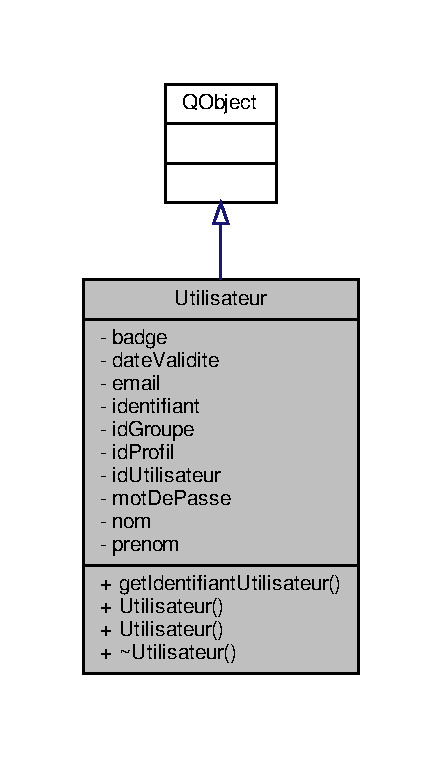
\includegraphics[width=212pt]{class_utilisateur__coll__graph}
\end{center}
\end{figure}
\subsubsection*{Fonctions membres publiques}
\begin{DoxyCompactItemize}
\item 
Q\+String \hyperlink{class_utilisateur_af944ac02cca7914480e20f46c4dd0e56}{get\+Identifiant\+Utilisateur} ()
\begin{DoxyCompactList}\small\item\em Définition de la méthode get\+Identifiant\+Utilisateur. \end{DoxyCompactList}\item 
\hyperlink{class_utilisateur_a89e539739c5f6c6790909ac5fc5729b8}{Utilisateur} (\hyperlink{class_q_object}{Q\+Object} $\ast$parent=nullptr)
\begin{DoxyCompactList}\small\item\em Constructeur de la classe \hyperlink{class_utilisateur}{Utilisateur}. \end{DoxyCompactList}\item 
\hyperlink{class_utilisateur_a6bfd9ef83e910946f3cf3b6e0fcca343}{Utilisateur} (Q\+String\+List donnees, \hyperlink{class_q_object}{Q\+Object} $\ast$parent=nullptr)
\begin{DoxyCompactList}\small\item\em Constructeur de la classe \hyperlink{class_utilisateur}{Utilisateur}. \end{DoxyCompactList}\item 
\hyperlink{class_utilisateur_a6631539ceecd6140fe525eb91485537b}{$\sim$\+Utilisateur} ()
\begin{DoxyCompactList}\small\item\em Destructeur de la classe \hyperlink{class_utilisateur}{Utilisateur}. \end{DoxyCompactList}\end{DoxyCompactItemize}
\subsubsection*{Attributs privés}
\begin{DoxyCompactItemize}
\item 
Q\+String \hyperlink{class_utilisateur_a77b48aa9d1f0ec04c69d45476897fec6}{badge}
\begin{DoxyCompactList}\small\item\em badge de l\textquotesingle{}utilisateur connecté \end{DoxyCompactList}\item 
Q\+String \hyperlink{class_utilisateur_a898cd6f5a64d733ad49a8a74388326cd}{date\+Validite}
\begin{DoxyCompactList}\small\item\em date\+Validite du compte \end{DoxyCompactList}\item 
Q\+String \hyperlink{class_utilisateur_a2f45443ce5277a5e6baefe5121e66555}{email}
\begin{DoxyCompactList}\small\item\em email de l\textquotesingle{}utilisateur connecté \end{DoxyCompactList}\item 
Q\+String \hyperlink{class_utilisateur_a1e79e47202a2c716346f47adbbeb2511}{identifiant}
\begin{DoxyCompactList}\small\item\em identifiant de l\textquotesingle{}utilisateur connecté \end{DoxyCompactList}\item 
Q\+String \hyperlink{class_utilisateur_a13c3425772da1d5501e6fe4a2f2b8194}{id\+Groupe}
\begin{DoxyCompactList}\small\item\em id\+Groupe de l\textquotesingle{}utilisateur connecté \end{DoxyCompactList}\item 
Q\+String \hyperlink{class_utilisateur_a042947e8b86637d1eb012c3fc89a959e}{id\+Profil}
\begin{DoxyCompactList}\small\item\em id\+Profil de l\textquotesingle{}utilisateur connecté \end{DoxyCompactList}\item 
Q\+String \hyperlink{class_utilisateur_ae1763e7a52c82c63506bc4160cdabb20}{id\+Utilisateur}
\begin{DoxyCompactList}\small\item\em id\+Utilisateur de l\textquotesingle{}utilisateur connecté \end{DoxyCompactList}\item 
Q\+String \hyperlink{class_utilisateur_a4f6a17d0fb5c231bcb414396236a056f}{mot\+De\+Passe}
\begin{DoxyCompactList}\small\item\em mot\+De\+Passe de l\textquotesingle{}utilisateur connecté \end{DoxyCompactList}\item 
Q\+String \hyperlink{class_utilisateur_a1096e809aca4b7cf453a7af93cb72502}{nom}
\begin{DoxyCompactList}\small\item\em nom de l\textquotesingle{}utilisateur connecté \end{DoxyCompactList}\item 
Q\+String \hyperlink{class_utilisateur_a1dd0779807b19298f30f39d9c371170f}{prenom}
\begin{DoxyCompactList}\small\item\em prenom de l\textquotesingle{}utilisateur connecté \end{DoxyCompactList}\end{DoxyCompactItemize}


\subsubsection{Description détaillée}
La classe \hyperlink{class_utilisateur}{Utilisateur} gère les données relative à l\textquotesingle{}utilisateur. 

\begin{DoxyAuthor}{Auteur}
Legger Pierre-\/\+Antoine
\end{DoxyAuthor}
\begin{DoxyVersion}{Version}
1.\+0
\end{DoxyVersion}
\begin{DoxyDate}{Date}
mercredi 04 Mars 2020 
\end{DoxyDate}


Définition à la ligne \hyperlink{_utilisateur_8h_source_l00052}{52} du fichier \hyperlink{_utilisateur_8h_source}{Utilisateur.\+h}.



\subsubsection{Documentation des constructeurs et destructeur}
\mbox{\Hypertarget{class_utilisateur_a89e539739c5f6c6790909ac5fc5729b8}\label{class_utilisateur_a89e539739c5f6c6790909ac5fc5729b8}} 
\index{Utilisateur@{Utilisateur}!Utilisateur@{Utilisateur}}
\index{Utilisateur@{Utilisateur}!Utilisateur@{Utilisateur}}
\paragraph{\texorpdfstring{Utilisateur()}{Utilisateur()}\hspace{0.1cm}{\footnotesize\ttfamily [1/2]}}
{\footnotesize\ttfamily Utilisateur\+::\+Utilisateur (\begin{DoxyParamCaption}\item[{\hyperlink{class_q_object}{Q\+Object} $\ast$}]{parent = {\ttfamily nullptr} }\end{DoxyParamCaption})}



Constructeur de la classe \hyperlink{class_utilisateur}{Utilisateur}. 

Initialise un objet \hyperlink{class_utilisateur}{Utilisateur} 
\begin{DoxyParams}{Paramètres}
{\em parent} & \\
\hline
\end{DoxyParams}


Définition à la ligne \hyperlink{_utilisateur_8cpp_source_l00022}{22} du fichier \hyperlink{_utilisateur_8cpp_source}{Utilisateur.\+cpp}.



Références \hyperlink{_utilisateur_8h_source_l00075}{badge}, \hyperlink{_utilisateur_8h_source_l00072}{date\+Validite}, \hyperlink{_utilisateur_8h_source_l00076}{email}, \hyperlink{_utilisateur_8h_source_l00073}{identifiant}, \hyperlink{_utilisateur_8h_source_l00069}{id\+Groupe}, \hyperlink{_utilisateur_8h_source_l00068}{id\+Profil}, \hyperlink{_utilisateur_8h_source_l00067}{id\+Utilisateur}, \hyperlink{_utilisateur_8h_source_l00074}{mot\+De\+Passe}, \hyperlink{_utilisateur_8h_source_l00070}{nom}, et \hyperlink{_utilisateur_8h_source_l00071}{prenom}.


\begin{DoxyCode}
00022                                         : \hyperlink{class_q_object}{QObject}(parent)
00023 \{
00024 \textcolor{preprocessor}{    #ifdef DEBUG\_UTILISATEUR}
00025         qDebug() << Q\_FUNC\_INFO;
00026 \textcolor{preprocessor}{    #endif}
00027     \hyperlink{class_utilisateur_ae1763e7a52c82c63506bc4160cdabb20}{idUtilisateur} = \textcolor{stringliteral}{""};
00028     \hyperlink{class_utilisateur_a042947e8b86637d1eb012c3fc89a959e}{idProfil} = \textcolor{stringliteral}{""};
00029     \hyperlink{class_utilisateur_a13c3425772da1d5501e6fe4a2f2b8194}{idGroupe} = \textcolor{stringliteral}{""};
00030     \hyperlink{class_utilisateur_a1096e809aca4b7cf453a7af93cb72502}{nom} = \textcolor{stringliteral}{""};
00031     \hyperlink{class_utilisateur_a1dd0779807b19298f30f39d9c371170f}{prenom} = \textcolor{stringliteral}{""};
00032     \hyperlink{class_utilisateur_a898cd6f5a64d733ad49a8a74388326cd}{dateValidite} = \textcolor{stringliteral}{""};
00033     \hyperlink{class_utilisateur_a1e79e47202a2c716346f47adbbeb2511}{identifiant} = \textcolor{stringliteral}{""};
00034     \hyperlink{class_utilisateur_a4f6a17d0fb5c231bcb414396236a056f}{motDePasse} = \textcolor{stringliteral}{""};
00035     \hyperlink{class_utilisateur_a77b48aa9d1f0ec04c69d45476897fec6}{badge} = \textcolor{stringliteral}{""};
00036     \hyperlink{class_utilisateur_a2f45443ce5277a5e6baefe5121e66555}{email} = \textcolor{stringliteral}{""};
00037 \}
\end{DoxyCode}
\mbox{\Hypertarget{class_utilisateur_a6bfd9ef83e910946f3cf3b6e0fcca343}\label{class_utilisateur_a6bfd9ef83e910946f3cf3b6e0fcca343}} 
\index{Utilisateur@{Utilisateur}!Utilisateur@{Utilisateur}}
\index{Utilisateur@{Utilisateur}!Utilisateur@{Utilisateur}}
\paragraph{\texorpdfstring{Utilisateur()}{Utilisateur()}\hspace{0.1cm}{\footnotesize\ttfamily [2/2]}}
{\footnotesize\ttfamily Utilisateur\+::\+Utilisateur (\begin{DoxyParamCaption}\item[{Q\+String\+List}]{donnees,  }\item[{\hyperlink{class_q_object}{Q\+Object} $\ast$}]{parent = {\ttfamily nullptr} }\end{DoxyParamCaption})}



Constructeur de la classe \hyperlink{class_utilisateur}{Utilisateur}. 

Initialise un objet \hyperlink{class_utilisateur}{Utilisateur} 
\begin{DoxyParams}{Paramètres}
{\em donnees} & \\
\hline
{\em parent} & \\
\hline
\end{DoxyParams}


Définition à la ligne \hyperlink{_utilisateur_8cpp_source_l00045}{45} du fichier \hyperlink{_utilisateur_8cpp_source}{Utilisateur.\+cpp}.



Références \hyperlink{_utilisateur_8h_source_l00075}{badge}, \hyperlink{_utilisateur_8h_source_l00072}{date\+Validite}, \hyperlink{_utilisateur_8h_source_l00076}{email}, \hyperlink{_utilisateur_8h_source_l00073}{identifiant}, \hyperlink{_utilisateur_8h_source_l00069}{id\+Groupe}, \hyperlink{_utilisateur_8h_source_l00068}{id\+Profil}, \hyperlink{_utilisateur_8h_source_l00067}{id\+Utilisateur}, \hyperlink{_utilisateur_8h_source_l00074}{mot\+De\+Passe}, \hyperlink{_utilisateur_8h_source_l00070}{nom}, \hyperlink{_utilisateur_8h_source_l00071}{prenom}, \hyperlink{_utilisateur_8h_source_l00035}{T\+A\+B\+L\+E\+\_\+\+U\+T\+I\+L\+I\+S\+A\+T\+E\+U\+R\+\_\+\+B\+A\+D\+GE}, \hyperlink{_utilisateur_8h_source_l00032}{T\+A\+B\+L\+E\+\_\+\+U\+T\+I\+L\+I\+S\+A\+T\+E\+U\+R\+\_\+\+D\+A\+T\+E\+\_\+\+V\+A\+L\+I\+D\+I\+TE}, \hyperlink{_utilisateur_8h_source_l00036}{T\+A\+B\+L\+E\+\_\+\+U\+T\+I\+L\+I\+S\+A\+T\+E\+U\+R\+\_\+\+E\+M\+A\+IL}, \hyperlink{_utilisateur_8h_source_l00029}{T\+A\+B\+L\+E\+\_\+\+U\+T\+I\+L\+I\+S\+A\+T\+E\+U\+R\+\_\+\+I\+D\+\_\+\+G\+R\+O\+U\+PE}, \hyperlink{_utilisateur_8h_source_l00028}{T\+A\+B\+L\+E\+\_\+\+U\+T\+I\+L\+I\+S\+A\+T\+E\+U\+R\+\_\+\+I\+D\+\_\+\+P\+R\+O\+F\+IL}, \hyperlink{_utilisateur_8h_source_l00027}{T\+A\+B\+L\+E\+\_\+\+U\+T\+I\+L\+I\+S\+A\+T\+E\+U\+R\+\_\+\+I\+D\+\_\+\+U\+T\+I\+L\+I\+S\+A\+T\+E\+UR}, \hyperlink{_utilisateur_8h_source_l00033}{T\+A\+B\+L\+E\+\_\+\+U\+T\+I\+L\+I\+S\+A\+T\+E\+U\+R\+\_\+\+I\+D\+E\+N\+T\+I\+F\+I\+A\+NT}, \hyperlink{_utilisateur_8h_source_l00034}{T\+A\+B\+L\+E\+\_\+\+U\+T\+I\+L\+I\+S\+A\+T\+E\+U\+R\+\_\+\+M\+O\+T\+\_\+\+D\+E\+\_\+\+P\+A\+S\+SE}, \hyperlink{_utilisateur_8h_source_l00030}{T\+A\+B\+L\+E\+\_\+\+U\+T\+I\+L\+I\+S\+A\+T\+E\+U\+R\+\_\+\+N\+OM}, et \hyperlink{_utilisateur_8h_source_l00031}{T\+A\+B\+L\+E\+\_\+\+U\+T\+I\+L\+I\+S\+A\+T\+E\+U\+R\+\_\+\+P\+R\+E\+N\+OM}.


\begin{DoxyCode}
00045                                                              : \hyperlink{class_q_object}{QObject}(parent)
00046 \{
00047 \textcolor{preprocessor}{    #ifdef DEBUG\_UTILISATEUR}
00048         qDebug() << Q\_FUNC\_INFO << donnees;
00049 \textcolor{preprocessor}{    #endif}
00050     \hyperlink{class_utilisateur_ae1763e7a52c82c63506bc4160cdabb20}{idUtilisateur} = donnees.at(\hyperlink{_utilisateur_8h_a2ee8bc4f44f3f2562a41638ec1d84ffcaf3d5820c10eaf883bc549062f87b1d29}{TABLE\_UTILISATEUR\_ID\_UTILISATEUR}
      );
00051     \hyperlink{class_utilisateur_a042947e8b86637d1eb012c3fc89a959e}{idProfil} = donnees.at(\hyperlink{_utilisateur_8h_a2ee8bc4f44f3f2562a41638ec1d84ffca4cc2b30f6bc705490fc4190e0d8668cc}{TABLE\_UTILISATEUR\_ID\_PROFIL});
00052     \hyperlink{class_utilisateur_a13c3425772da1d5501e6fe4a2f2b8194}{idGroupe} = donnees.at(\hyperlink{_utilisateur_8h_a2ee8bc4f44f3f2562a41638ec1d84ffcaafd6ac7708481835f0c9aa3dbcddd1e8}{TABLE\_UTILISATEUR\_ID\_GROUPE});
00053     \hyperlink{class_utilisateur_a1096e809aca4b7cf453a7af93cb72502}{nom} = donnees.at(\hyperlink{_utilisateur_8h_a2ee8bc4f44f3f2562a41638ec1d84ffca79ab7400bfc906a77d1f56988349ebd4}{TABLE\_UTILISATEUR\_NOM});
00054     \hyperlink{class_utilisateur_a1dd0779807b19298f30f39d9c371170f}{prenom} = donnees.at(\hyperlink{_utilisateur_8h_a2ee8bc4f44f3f2562a41638ec1d84ffcab8ef43f3428ce1b6a50b1f15e6771d75}{TABLE\_UTILISATEUR\_PRENOM});
00055     \hyperlink{class_utilisateur_a898cd6f5a64d733ad49a8a74388326cd}{dateValidite} = donnees.at(\hyperlink{_utilisateur_8h_a2ee8bc4f44f3f2562a41638ec1d84ffca1a0604e4b99c353c04b8ee64a2524cca}{TABLE\_UTILISATEUR\_DATE\_VALIDITE});
00056     \hyperlink{class_utilisateur_a1e79e47202a2c716346f47adbbeb2511}{identifiant} = donnees.at(\hyperlink{_utilisateur_8h_a2ee8bc4f44f3f2562a41638ec1d84ffca00d7c04c0ac35952230b782d3cdb4942}{TABLE\_UTILISATEUR\_IDENTIFIANT});
00057     \hyperlink{class_utilisateur_a4f6a17d0fb5c231bcb414396236a056f}{motDePasse} = donnees.at(\hyperlink{_utilisateur_8h_a2ee8bc4f44f3f2562a41638ec1d84ffca09688a0481708cf5d77cd6a438d12623}{TABLE\_UTILISATEUR\_MOT\_DE\_PASSE});
00058     \hyperlink{class_utilisateur_a77b48aa9d1f0ec04c69d45476897fec6}{badge} = donnees.at(\hyperlink{_utilisateur_8h_a2ee8bc4f44f3f2562a41638ec1d84ffca9d0825de5c0afa69202e7773e7e10d1f}{TABLE\_UTILISATEUR\_BADGE});
00059     \hyperlink{class_utilisateur_a2f45443ce5277a5e6baefe5121e66555}{email} = donnees.at(\hyperlink{_utilisateur_8h_a2ee8bc4f44f3f2562a41638ec1d84ffca64c38d44af4e843f5930551e5ac1733f}{TABLE\_UTILISATEUR\_EMAIL});
00060 \}
\end{DoxyCode}
\mbox{\Hypertarget{class_utilisateur_a6631539ceecd6140fe525eb91485537b}\label{class_utilisateur_a6631539ceecd6140fe525eb91485537b}} 
\index{Utilisateur@{Utilisateur}!````~Utilisateur@{$\sim$\+Utilisateur}}
\index{````~Utilisateur@{$\sim$\+Utilisateur}!Utilisateur@{Utilisateur}}
\paragraph{\texorpdfstring{$\sim$\+Utilisateur()}{~Utilisateur()}}
{\footnotesize\ttfamily Utilisateur\+::$\sim$\+Utilisateur (\begin{DoxyParamCaption}{ }\end{DoxyParamCaption})}



Destructeur de la classe \hyperlink{class_utilisateur}{Utilisateur}. 

Détruit un objet \hyperlink{class_utilisateur}{Utilisateur} 

Définition à la ligne \hyperlink{_utilisateur_8cpp_source_l00067}{67} du fichier \hyperlink{_utilisateur_8cpp_source}{Utilisateur.\+cpp}.


\begin{DoxyCode}
00068 \{
00069 
00070 \}
\end{DoxyCode}


\subsubsection{Documentation des fonctions membres}
\mbox{\Hypertarget{class_utilisateur_af944ac02cca7914480e20f46c4dd0e56}\label{class_utilisateur_af944ac02cca7914480e20f46c4dd0e56}} 
\index{Utilisateur@{Utilisateur}!get\+Identifiant\+Utilisateur@{get\+Identifiant\+Utilisateur}}
\index{get\+Identifiant\+Utilisateur@{get\+Identifiant\+Utilisateur}!Utilisateur@{Utilisateur}}
\paragraph{\texorpdfstring{get\+Identifiant\+Utilisateur()}{getIdentifiantUtilisateur()}}
{\footnotesize\ttfamily Q\+String Utilisateur\+::get\+Identifiant\+Utilisateur (\begin{DoxyParamCaption}{ }\end{DoxyParamCaption})}



Définition de la méthode get\+Identifiant\+Utilisateur. 

retourne les identifiant de l\textquotesingle{}utilisateur \begin{DoxyReturn}{Renvoie}
les identifiants 
\end{DoxyReturn}


Définition à la ligne \hyperlink{_utilisateur_8cpp_source_l00078}{78} du fichier \hyperlink{_utilisateur_8cpp_source}{Utilisateur.\+cpp}.



Références \hyperlink{_utilisateur_8h_source_l00070}{nom}, et \hyperlink{_utilisateur_8h_source_l00071}{prenom}.



Référencé par \hyperlink{_supervision_8cpp_source_l00256}{Supervision\+::connecter\+Utilisateur()}.


\begin{DoxyCode}
00079 \{
00080     \textcolor{keywordflow}{return} \hyperlink{class_utilisateur_a1096e809aca4b7cf453a7af93cb72502}{nom} + \textcolor{stringliteral}{" "} + \hyperlink{class_utilisateur_a1dd0779807b19298f30f39d9c371170f}{prenom};
00081 \}
\end{DoxyCode}


\subsubsection{Documentation des données membres}
\mbox{\Hypertarget{class_utilisateur_a77b48aa9d1f0ec04c69d45476897fec6}\label{class_utilisateur_a77b48aa9d1f0ec04c69d45476897fec6}} 
\index{Utilisateur@{Utilisateur}!badge@{badge}}
\index{badge@{badge}!Utilisateur@{Utilisateur}}
\paragraph{\texorpdfstring{badge}{badge}}
{\footnotesize\ttfamily Q\+String Utilisateur\+::badge\hspace{0.3cm}{\ttfamily [private]}}



badge de l\textquotesingle{}utilisateur connecté 



Définition à la ligne \hyperlink{_utilisateur_8h_source_l00075}{75} du fichier \hyperlink{_utilisateur_8h_source}{Utilisateur.\+h}.



Référencé par \hyperlink{_utilisateur_8cpp_source_l00022}{Utilisateur()}.

\mbox{\Hypertarget{class_utilisateur_a898cd6f5a64d733ad49a8a74388326cd}\label{class_utilisateur_a898cd6f5a64d733ad49a8a74388326cd}} 
\index{Utilisateur@{Utilisateur}!date\+Validite@{date\+Validite}}
\index{date\+Validite@{date\+Validite}!Utilisateur@{Utilisateur}}
\paragraph{\texorpdfstring{date\+Validite}{dateValidite}}
{\footnotesize\ttfamily Q\+String Utilisateur\+::date\+Validite\hspace{0.3cm}{\ttfamily [private]}}



date\+Validite du compte 



Définition à la ligne \hyperlink{_utilisateur_8h_source_l00072}{72} du fichier \hyperlink{_utilisateur_8h_source}{Utilisateur.\+h}.



Référencé par \hyperlink{_utilisateur_8cpp_source_l00022}{Utilisateur()}.

\mbox{\Hypertarget{class_utilisateur_a2f45443ce5277a5e6baefe5121e66555}\label{class_utilisateur_a2f45443ce5277a5e6baefe5121e66555}} 
\index{Utilisateur@{Utilisateur}!email@{email}}
\index{email@{email}!Utilisateur@{Utilisateur}}
\paragraph{\texorpdfstring{email}{email}}
{\footnotesize\ttfamily Q\+String Utilisateur\+::email\hspace{0.3cm}{\ttfamily [private]}}



email de l\textquotesingle{}utilisateur connecté 



Définition à la ligne \hyperlink{_utilisateur_8h_source_l00076}{76} du fichier \hyperlink{_utilisateur_8h_source}{Utilisateur.\+h}.



Référencé par \hyperlink{_utilisateur_8cpp_source_l00022}{Utilisateur()}.

\mbox{\Hypertarget{class_utilisateur_a1e79e47202a2c716346f47adbbeb2511}\label{class_utilisateur_a1e79e47202a2c716346f47adbbeb2511}} 
\index{Utilisateur@{Utilisateur}!identifiant@{identifiant}}
\index{identifiant@{identifiant}!Utilisateur@{Utilisateur}}
\paragraph{\texorpdfstring{identifiant}{identifiant}}
{\footnotesize\ttfamily Q\+String Utilisateur\+::identifiant\hspace{0.3cm}{\ttfamily [private]}}



identifiant de l\textquotesingle{}utilisateur connecté 



Définition à la ligne \hyperlink{_utilisateur_8h_source_l00073}{73} du fichier \hyperlink{_utilisateur_8h_source}{Utilisateur.\+h}.



Référencé par \hyperlink{_utilisateur_8cpp_source_l00022}{Utilisateur()}.

\mbox{\Hypertarget{class_utilisateur_a13c3425772da1d5501e6fe4a2f2b8194}\label{class_utilisateur_a13c3425772da1d5501e6fe4a2f2b8194}} 
\index{Utilisateur@{Utilisateur}!id\+Groupe@{id\+Groupe}}
\index{id\+Groupe@{id\+Groupe}!Utilisateur@{Utilisateur}}
\paragraph{\texorpdfstring{id\+Groupe}{idGroupe}}
{\footnotesize\ttfamily Q\+String Utilisateur\+::id\+Groupe\hspace{0.3cm}{\ttfamily [private]}}



id\+Groupe de l\textquotesingle{}utilisateur connecté 



Définition à la ligne \hyperlink{_utilisateur_8h_source_l00069}{69} du fichier \hyperlink{_utilisateur_8h_source}{Utilisateur.\+h}.



Référencé par \hyperlink{_utilisateur_8cpp_source_l00022}{Utilisateur()}.

\mbox{\Hypertarget{class_utilisateur_a042947e8b86637d1eb012c3fc89a959e}\label{class_utilisateur_a042947e8b86637d1eb012c3fc89a959e}} 
\index{Utilisateur@{Utilisateur}!id\+Profil@{id\+Profil}}
\index{id\+Profil@{id\+Profil}!Utilisateur@{Utilisateur}}
\paragraph{\texorpdfstring{id\+Profil}{idProfil}}
{\footnotesize\ttfamily Q\+String Utilisateur\+::id\+Profil\hspace{0.3cm}{\ttfamily [private]}}



id\+Profil de l\textquotesingle{}utilisateur connecté 



Définition à la ligne \hyperlink{_utilisateur_8h_source_l00068}{68} du fichier \hyperlink{_utilisateur_8h_source}{Utilisateur.\+h}.



Référencé par \hyperlink{_utilisateur_8cpp_source_l00022}{Utilisateur()}.

\mbox{\Hypertarget{class_utilisateur_ae1763e7a52c82c63506bc4160cdabb20}\label{class_utilisateur_ae1763e7a52c82c63506bc4160cdabb20}} 
\index{Utilisateur@{Utilisateur}!id\+Utilisateur@{id\+Utilisateur}}
\index{id\+Utilisateur@{id\+Utilisateur}!Utilisateur@{Utilisateur}}
\paragraph{\texorpdfstring{id\+Utilisateur}{idUtilisateur}}
{\footnotesize\ttfamily Q\+String Utilisateur\+::id\+Utilisateur\hspace{0.3cm}{\ttfamily [private]}}



id\+Utilisateur de l\textquotesingle{}utilisateur connecté 



Définition à la ligne \hyperlink{_utilisateur_8h_source_l00067}{67} du fichier \hyperlink{_utilisateur_8h_source}{Utilisateur.\+h}.



Référencé par \hyperlink{_utilisateur_8cpp_source_l00022}{Utilisateur()}.

\mbox{\Hypertarget{class_utilisateur_a4f6a17d0fb5c231bcb414396236a056f}\label{class_utilisateur_a4f6a17d0fb5c231bcb414396236a056f}} 
\index{Utilisateur@{Utilisateur}!mot\+De\+Passe@{mot\+De\+Passe}}
\index{mot\+De\+Passe@{mot\+De\+Passe}!Utilisateur@{Utilisateur}}
\paragraph{\texorpdfstring{mot\+De\+Passe}{motDePasse}}
{\footnotesize\ttfamily Q\+String Utilisateur\+::mot\+De\+Passe\hspace{0.3cm}{\ttfamily [private]}}



mot\+De\+Passe de l\textquotesingle{}utilisateur connecté 



Définition à la ligne \hyperlink{_utilisateur_8h_source_l00074}{74} du fichier \hyperlink{_utilisateur_8h_source}{Utilisateur.\+h}.



Référencé par \hyperlink{_utilisateur_8cpp_source_l00022}{Utilisateur()}.

\mbox{\Hypertarget{class_utilisateur_a1096e809aca4b7cf453a7af93cb72502}\label{class_utilisateur_a1096e809aca4b7cf453a7af93cb72502}} 
\index{Utilisateur@{Utilisateur}!nom@{nom}}
\index{nom@{nom}!Utilisateur@{Utilisateur}}
\paragraph{\texorpdfstring{nom}{nom}}
{\footnotesize\ttfamily Q\+String Utilisateur\+::nom\hspace{0.3cm}{\ttfamily [private]}}



nom de l\textquotesingle{}utilisateur connecté 



Définition à la ligne \hyperlink{_utilisateur_8h_source_l00070}{70} du fichier \hyperlink{_utilisateur_8h_source}{Utilisateur.\+h}.



Référencé par \hyperlink{_utilisateur_8cpp_source_l00078}{get\+Identifiant\+Utilisateur()}, et \hyperlink{_utilisateur_8cpp_source_l00022}{Utilisateur()}.

\mbox{\Hypertarget{class_utilisateur_a1dd0779807b19298f30f39d9c371170f}\label{class_utilisateur_a1dd0779807b19298f30f39d9c371170f}} 
\index{Utilisateur@{Utilisateur}!prenom@{prenom}}
\index{prenom@{prenom}!Utilisateur@{Utilisateur}}
\paragraph{\texorpdfstring{prenom}{prenom}}
{\footnotesize\ttfamily Q\+String Utilisateur\+::prenom\hspace{0.3cm}{\ttfamily [private]}}



prenom de l\textquotesingle{}utilisateur connecté 



Définition à la ligne \hyperlink{_utilisateur_8h_source_l00071}{71} du fichier \hyperlink{_utilisateur_8h_source}{Utilisateur.\+h}.



Référencé par \hyperlink{_utilisateur_8cpp_source_l00078}{get\+Identifiant\+Utilisateur()}, et \hyperlink{_utilisateur_8cpp_source_l00022}{Utilisateur()}.



La documentation de cette classe a été générée à partir des fichiers suivants \+:\begin{DoxyCompactItemize}
\item 
\hyperlink{_utilisateur_8h}{Utilisateur.\+h}\item 
\hyperlink{_utilisateur_8cpp}{Utilisateur.\+cpp}\end{DoxyCompactItemize}

\section{Documentation des fichiers}
\hypertarget{_armoire_8cpp}{}\subsection{Référence du fichier Armoire.\+cpp}
\label{_armoire_8cpp}\index{Armoire.\+cpp@{Armoire.\+cpp}}


Définition de la classe \hyperlink{class_armoire}{Armoire}.  


{\ttfamily \#include \char`\"{}Armoire.\+h\char`\"{}}\newline
{\ttfamily \#include \char`\"{}Bdd.\+h\char`\"{}}\newline
{\ttfamily \#include $<$Q\+Network\+Interface$>$}\newline


\subsubsection{Description détaillée}
Définition de la classe \hyperlink{class_armoire}{Armoire}. 

\begin{DoxyAuthor}{Auteur}
Tranchat Joffrey
\end{DoxyAuthor}
\begin{DoxyVersion}{Version}
1.\+0
\end{DoxyVersion}
\begin{DoxyDate}{Date}
22 Mars 2020 
\end{DoxyDate}


Définition dans le fichier \hyperlink{_armoire_8cpp_source}{Armoire.\+cpp}.


\hypertarget{_armoire_8cpp_source}{}\subsection{Armoire.\+cpp}
\label{_armoire_8cpp_source}\index{Armoire.\+cpp@{Armoire.\+cpp}}

\begin{DoxyCode}
00001 \textcolor{preprocessor}{#include "\hyperlink{_armoire_8h}{Armoire.h}"}
00002 \textcolor{preprocessor}{#include "\hyperlink{_bdd_8h}{Bdd.h}"}
00003 \textcolor{preprocessor}{#include <QNetworkInterface>}
00004 
\Hypertarget{_armoire_8cpp_source_l00022}\hyperlink{class_armoire_a5db260c682a9d2688afc0efbd5be8d14}{00022} \hyperlink{class_armoire_a5db260c682a9d2688afc0efbd5be8d14}{Armoire::Armoire}(\hyperlink{class_q_object}{QObject} *parent) : \hyperlink{class_q_object}{QObject}(parent)
00023 \{
00024 \textcolor{preprocessor}{    #ifdef DEBUG\_ARMOIRE}
00025         qDebug() << Q\_FUNC\_INFO;
00026 \textcolor{preprocessor}{    #endif}
00027     \hyperlink{class_armoire_a555f656018e7b600987128cdc792e320}{bdd} = \hyperlink{class_bdd_a6f55c29d593da12ca31fad02f5adfe24}{Bdd::getInstance}();
00028     \hyperlink{class_armoire_ab96bd042aa78eaefba0aefb860684ca6}{adresseIPArmoire} = \hyperlink{class_armoire_abc30649cc7d4f3c0cefcc54894aeb406}{lireAdresseIP}();
00029     \hyperlink{class_armoire_a1c5266f9e4b01c0d2e1d244d2f11fffd}{recupererArmoire}();
00030 \}
00031 
\Hypertarget{_armoire_8cpp_source_l00036}\hyperlink{class_armoire_a0f506a879391a987f12f59a23f60634e}{00036} \hyperlink{class_armoire_a0f506a879391a987f12f59a23f60634e}{Armoire::~Armoire}()
00037 \{
00038     \hyperlink{class_bdd_af89fa3ffa107c7859a3964bf032cfdb7}{Bdd::detruireInstance}();
00039 \textcolor{preprocessor}{    #ifdef DEBUG\_ARMOIRE}
00040         qDebug() << Q\_FUNC\_INFO;
00041 \textcolor{preprocessor}{    #endif}
00042 \}
00043 
\Hypertarget{_armoire_8cpp_source_l00049}\hyperlink{class_armoire_a1c5266f9e4b01c0d2e1d244d2f11fffd}{00049} \textcolor{keywordtype}{void} \hyperlink{class_armoire_a1c5266f9e4b01c0d2e1d244d2f11fffd}{Armoire::recupererArmoire}(QString \hyperlink{class_armoire_a131caceb7d4b90cb7761851757e80f57}{idArmoire})
00050 \{
00051     QString requeteBDD;
00052 
00053     \textcolor{keywordflow}{if}(!idArmoire.isEmpty()) \textcolor{comment}{// par id}
00054     \{
00055         requeteBDD = \textcolor{stringliteral}{"SELECT * from Armoire where idArmoire = '"} + idArmoire + \textcolor{stringliteral}{"'"};
00056         QStringList donnees;
00057         \hyperlink{class_armoire_a555f656018e7b600987128cdc792e320}{bdd}->\hyperlink{class_bdd_a8f25d29d309041bbf875700db0efd97b}{recuperer}(requeteBDD, donnees);
00058 
00059 \textcolor{preprocessor}{        #ifdef DEBUG\_ARMOIRE}
00060             qDebug() << Q\_FUNC\_INFO << donnees;
00061 \textcolor{preprocessor}{        #endif}
00062 
00063         \textcolor{keywordflow}{if}(donnees.size() > 0)
00064         \{
00065             this->idArmoire = donnees.at(\hyperlink{_armoire_8h_a8c8e83929e4df868beea17eda4fb5dada167bbea3f9d799583c77d0a6b12ed99e}{TABLE\_ARMOIRE\_ID\_ARMOIRE});
00066             \hyperlink{class_armoire_a1de028da0fa3f085e2feaad8311d8795}{nom} = donnees.at(\hyperlink{_armoire_8h_a8c8e83929e4df868beea17eda4fb5dadaed87f53039b2f5f5401a4b4c9ea8a706}{TABLE\_ARMOIRE\_NOM});
00067             \hyperlink{class_armoire_aa18be328693d7602439c779e30156c02}{description} = donnees.at(\hyperlink{_armoire_8h_a8c8e83929e4df868beea17eda4fb5dadaa46613f3c7eb048c8392fb780e801cc8}{TABLE\_ARMOIRE\_DESCRIPTION});
00068             \hyperlink{class_armoire_a9c4e926b7cddb13d097b75b3f5ef3de8}{nbCasiers} = donnees.at(\hyperlink{_armoire_8h_a8c8e83929e4df868beea17eda4fb5dada92634af3316ad54be209ef14cc8a8981}{TABLE\_ARMOIRE\_NB\_CASIERS});
00069         \}
00070     \}    
00071 \}
00072 
\Hypertarget{_armoire_8cpp_source_l00078}\hyperlink{class_armoire_a3e4d2ffc2fb91dd24d1160305ad36555}{00078} QStringList \hyperlink{class_armoire_a3e4d2ffc2fb91dd24d1160305ad36555}{Armoire::getInformations}()
00079 \{
00080     QStringList informations;
00081 
00082     informations << \hyperlink{class_armoire_a131caceb7d4b90cb7761851757e80f57}{idArmoire} << \hyperlink{class_armoire_a1de028da0fa3f085e2feaad8311d8795}{nom} << \hyperlink{class_armoire_aa18be328693d7602439c779e30156c02}{description} << 
      \hyperlink{class_armoire_a9c4e926b7cddb13d097b75b3f5ef3de8}{nbCasiers} << \hyperlink{class_armoire_ab96bd042aa78eaefba0aefb860684ca6}{adresseIPArmoire};
00083 
00084     emit \hyperlink{class_armoire_a1fc00ceaa842f579ee31c532a9b01508}{informationsArmoire}(informations);
00085 
00086     \textcolor{keywordflow}{return} informations;
00087 \}
00088 
\Hypertarget{_armoire_8cpp_source_l00094}\hyperlink{class_armoire_a1a76e497170632b30f9821b396d53cec}{00094} QString \hyperlink{class_armoire_a1a76e497170632b30f9821b396d53cec}{Armoire::getIdArmoire}()\textcolor{keyword}{ const}
00095 \textcolor{keyword}{}\{
00096     \textcolor{keywordflow}{return} \hyperlink{class_armoire_a131caceb7d4b90cb7761851757e80f57}{idArmoire};
00097 \}
00098 
\Hypertarget{_armoire_8cpp_source_l00105}\hyperlink{class_armoire_a0045e45e0c9a465af765667344ce8bee}{00105} QString \hyperlink{class_armoire_a0045e45e0c9a465af765667344ce8bee}{Armoire::getNom}()\textcolor{keyword}{ const}
00106 \textcolor{keyword}{}\{
00107     \textcolor{keywordflow}{return} \hyperlink{class_armoire_a1de028da0fa3f085e2feaad8311d8795}{nom};
00108 \}
00109 
\Hypertarget{_armoire_8cpp_source_l00116}\hyperlink{class_armoire_a19af26aa7dedd03202d2484744dcad76}{00116} QString \hyperlink{class_armoire_a19af26aa7dedd03202d2484744dcad76}{Armoire::getDescripton}()\textcolor{keyword}{ const}
00117 \textcolor{keyword}{}\{
00118     \textcolor{keywordflow}{return} \hyperlink{class_armoire_aa18be328693d7602439c779e30156c02}{description};
00119 \}
00120 
\Hypertarget{_armoire_8cpp_source_l00127}\hyperlink{class_armoire_aa94faaf53b6da5139a22a2ab21d4cf12}{00127} QString \hyperlink{class_armoire_aa94faaf53b6da5139a22a2ab21d4cf12}{Armoire::getNbCasiers}()\textcolor{keyword}{ const}
00128 \textcolor{keyword}{}\{
00129     \textcolor{keywordflow}{return} \hyperlink{class_armoire_a9c4e926b7cddb13d097b75b3f5ef3de8}{nbCasiers};
00130 \}
00131 
\Hypertarget{_armoire_8cpp_source_l00138}\hyperlink{class_armoire_a706def736570580d7e5e3d2e29321c66}{00138} QString \hyperlink{class_armoire_a706def736570580d7e5e3d2e29321c66}{Armoire::getAdresseIPArmoire}()\textcolor{keyword}{ const}
00139 \textcolor{keyword}{}\{
00140     \textcolor{keywordflow}{return} \hyperlink{class_armoire_ab96bd042aa78eaefba0aefb860684ca6}{adresseIPArmoire};
00141 \}
00142 
\Hypertarget{_armoire_8cpp_source_l00149}\hyperlink{class_armoire_abc30649cc7d4f3c0cefcc54894aeb406}{00149} QString \hyperlink{class_armoire_abc30649cc7d4f3c0cefcc54894aeb406}{Armoire::lireAdresseIP}()
00150 \{
00151     QStringList adresses;
00152     \textcolor{keywordflow}{foreach}(QHostAddress adresse, QNetworkInterface::allAddresses())
00153     \{
00154         \textcolor{comment}{// Filtre les adresses localhost ...}
00155         \textcolor{keywordflow}{if}(adresse != QHostAddress::LocalHostIPv6
00156            && adresse != QHostAddress::LocalHost
00157            \textcolor{comment}{// ... APIPA ...}
00158            && !adresse.isInSubnet(QHostAddress::parseSubnet(\textcolor{stringliteral}{"169.254.0.0/16"}))
00159            \textcolor{comment}{// ... Lien Local IPv6}
00160            && !adresse.isInSubnet(QHostAddress::parseSubnet(\textcolor{stringliteral}{"FE80::/64"})))
00161         \{
00162             qDebug() << Q\_FUNC\_INFO << adresse.toString();
00163             adresses << adresse.toString();
00164         \}
00165     \}
00166 
00167     \textcolor{keywordflow}{foreach}(QString adresse, adresses)
00168     \{
00169 \textcolor{preprocessor}{        #ifdef DEBUG\_ARMOIRE}
00170             qDebug() << Q\_FUNC\_INFO << adresse;
00171 \textcolor{preprocessor}{        #endif}
00172         \textcolor{keywordflow}{if}(adresse.contains(\textcolor{stringliteral}{"192."}))
00173             \textcolor{keywordflow}{return} adresse;
00174     \}
00175 
00176     \textcolor{comment}{/*if(adresses.count() > 0)}
00177 \textcolor{comment}{    \{}
00178 \textcolor{comment}{        return adresses.at(0);}
00179 \textcolor{comment}{    \}*/}
00180 
00181     \textcolor{keywordflow}{return} QString(\textcolor{stringliteral}{""});
00182 \}
\end{DoxyCode}

\hypertarget{_armoire_8h}{}\subsection{Référence du fichier Armoire.\+h}
\label{_armoire_8h}\index{Armoire.\+h@{Armoire.\+h}}


Déclaration de la classe \hyperlink{class_armoire}{Armoire}.  


{\ttfamily \#include $<$Q\+Object$>$}\newline
{\ttfamily \#include $<$Q\+String$>$}\newline
{\ttfamily \#include $<$Q\+Debug$>$}\newline
\subsubsection*{Classes}
\begin{DoxyCompactItemize}
\item 
class \hyperlink{class_armoire}{Armoire}
\begin{DoxyCompactList}\small\item\em La classe \hyperlink{class_armoire}{Armoire} traite les articles. \end{DoxyCompactList}\end{DoxyCompactItemize}
\subsubsection*{Macros}
\begin{DoxyCompactItemize}
\item 
\#define \hyperlink{_armoire_8h_a15e7936003b0c10a4cf49799119463ab}{D\+E\+B\+U\+G\+\_\+\+A\+R\+M\+O\+I\+RE}
\end{DoxyCompactItemize}
\subsubsection*{Énumérations}
\begin{DoxyCompactItemize}
\item 
enum \hyperlink{_armoire_8h_a8c8e83929e4df868beea17eda4fb5dad}{Champ\+Armoire} \{ \hyperlink{_armoire_8h_a8c8e83929e4df868beea17eda4fb5dada167bbea3f9d799583c77d0a6b12ed99e}{T\+A\+B\+L\+E\+\_\+\+A\+R\+M\+O\+I\+R\+E\+\_\+\+I\+D\+\_\+\+A\+R\+M\+O\+I\+RE}, 
\hyperlink{_armoire_8h_a8c8e83929e4df868beea17eda4fb5dadaed87f53039b2f5f5401a4b4c9ea8a706}{T\+A\+B\+L\+E\+\_\+\+A\+R\+M\+O\+I\+R\+E\+\_\+\+N\+OM}, 
\hyperlink{_armoire_8h_a8c8e83929e4df868beea17eda4fb5dadaa46613f3c7eb048c8392fb780e801cc8}{T\+A\+B\+L\+E\+\_\+\+A\+R\+M\+O\+I\+R\+E\+\_\+\+D\+E\+S\+C\+R\+I\+P\+T\+I\+ON}, 
\hyperlink{_armoire_8h_a8c8e83929e4df868beea17eda4fb5dada92634af3316ad54be209ef14cc8a8981}{T\+A\+B\+L\+E\+\_\+\+A\+R\+M\+O\+I\+R\+E\+\_\+\+N\+B\+\_\+\+C\+A\+S\+I\+E\+RS}
 \}\begin{DoxyCompactList}\small\item\em Définit les différents champs de la table \hyperlink{class_armoire}{Armoire}. \end{DoxyCompactList}
\end{DoxyCompactItemize}


\subsubsection{Description détaillée}
Déclaration de la classe \hyperlink{class_armoire}{Armoire}. 

\begin{DoxyAuthor}{Auteur}
Tranchat Joffrey
\end{DoxyAuthor}
\begin{DoxyVersion}{Version}
1.\+0
\end{DoxyVersion}
\begin{DoxyDate}{Date}
Dimanche 22 Mars 2020 
\end{DoxyDate}


Définition dans le fichier \hyperlink{_armoire_8h_source}{Armoire.\+h}.



\subsubsection{Documentation des macros}
\mbox{\Hypertarget{_armoire_8h_a15e7936003b0c10a4cf49799119463ab}\label{_armoire_8h_a15e7936003b0c10a4cf49799119463ab}} 
\index{Armoire.\+h@{Armoire.\+h}!D\+E\+B\+U\+G\+\_\+\+A\+R\+M\+O\+I\+RE@{D\+E\+B\+U\+G\+\_\+\+A\+R\+M\+O\+I\+RE}}
\index{D\+E\+B\+U\+G\+\_\+\+A\+R\+M\+O\+I\+RE@{D\+E\+B\+U\+G\+\_\+\+A\+R\+M\+O\+I\+RE}!Armoire.\+h@{Armoire.\+h}}
\paragraph{\texorpdfstring{D\+E\+B\+U\+G\+\_\+\+A\+R\+M\+O\+I\+RE}{DEBUG\_ARMOIRE}}
{\footnotesize\ttfamily \#define D\+E\+B\+U\+G\+\_\+\+A\+R\+M\+O\+I\+RE}



Définition à la ligne \hyperlink{_armoire_8h_source_l00021}{21} du fichier \hyperlink{_armoire_8h_source}{Armoire.\+h}.



\subsubsection{Documentation du type de l\textquotesingle{}énumération}
\mbox{\Hypertarget{_armoire_8h_a8c8e83929e4df868beea17eda4fb5dad}\label{_armoire_8h_a8c8e83929e4df868beea17eda4fb5dad}} 
\index{Armoire.\+h@{Armoire.\+h}!Champ\+Armoire@{Champ\+Armoire}}
\index{Champ\+Armoire@{Champ\+Armoire}!Armoire.\+h@{Armoire.\+h}}
\paragraph{\texorpdfstring{Champ\+Armoire}{ChampArmoire}}
{\footnotesize\ttfamily enum \hyperlink{_armoire_8h_a8c8e83929e4df868beea17eda4fb5dad}{Champ\+Armoire}}



Définit les différents champs de la table \hyperlink{class_armoire}{Armoire}. 

\begin{DoxyEnumFields}{Valeurs énumérées}
\raisebox{\heightof{T}}[0pt][0pt]{\index{T\+A\+B\+L\+E\+\_\+\+A\+R\+M\+O\+I\+R\+E\+\_\+\+I\+D\+\_\+\+A\+R\+M\+O\+I\+RE@{T\+A\+B\+L\+E\+\_\+\+A\+R\+M\+O\+I\+R\+E\+\_\+\+I\+D\+\_\+\+A\+R\+M\+O\+I\+RE}!Armoire.\+h@{Armoire.\+h}}\index{Armoire.\+h@{Armoire.\+h}!T\+A\+B\+L\+E\+\_\+\+A\+R\+M\+O\+I\+R\+E\+\_\+\+I\+D\+\_\+\+A\+R\+M\+O\+I\+RE@{T\+A\+B\+L\+E\+\_\+\+A\+R\+M\+O\+I\+R\+E\+\_\+\+I\+D\+\_\+\+A\+R\+M\+O\+I\+RE}}}\mbox{\Hypertarget{_armoire_8h_a8c8e83929e4df868beea17eda4fb5dada167bbea3f9d799583c77d0a6b12ed99e}\label{_armoire_8h_a8c8e83929e4df868beea17eda4fb5dada167bbea3f9d799583c77d0a6b12ed99e}} 
T\+A\+B\+L\+E\+\_\+\+A\+R\+M\+O\+I\+R\+E\+\_\+\+I\+D\+\_\+\+A\+R\+M\+O\+I\+RE&\\
\hline

\raisebox{\heightof{T}}[0pt][0pt]{\index{T\+A\+B\+L\+E\+\_\+\+A\+R\+M\+O\+I\+R\+E\+\_\+\+N\+OM@{T\+A\+B\+L\+E\+\_\+\+A\+R\+M\+O\+I\+R\+E\+\_\+\+N\+OM}!Armoire.\+h@{Armoire.\+h}}\index{Armoire.\+h@{Armoire.\+h}!T\+A\+B\+L\+E\+\_\+\+A\+R\+M\+O\+I\+R\+E\+\_\+\+N\+OM@{T\+A\+B\+L\+E\+\_\+\+A\+R\+M\+O\+I\+R\+E\+\_\+\+N\+OM}}}\mbox{\Hypertarget{_armoire_8h_a8c8e83929e4df868beea17eda4fb5dadaed87f53039b2f5f5401a4b4c9ea8a706}\label{_armoire_8h_a8c8e83929e4df868beea17eda4fb5dadaed87f53039b2f5f5401a4b4c9ea8a706}} 
T\+A\+B\+L\+E\+\_\+\+A\+R\+M\+O\+I\+R\+E\+\_\+\+N\+OM&\\
\hline

\raisebox{\heightof{T}}[0pt][0pt]{\index{T\+A\+B\+L\+E\+\_\+\+A\+R\+M\+O\+I\+R\+E\+\_\+\+D\+E\+S\+C\+R\+I\+P\+T\+I\+ON@{T\+A\+B\+L\+E\+\_\+\+A\+R\+M\+O\+I\+R\+E\+\_\+\+D\+E\+S\+C\+R\+I\+P\+T\+I\+ON}!Armoire.\+h@{Armoire.\+h}}\index{Armoire.\+h@{Armoire.\+h}!T\+A\+B\+L\+E\+\_\+\+A\+R\+M\+O\+I\+R\+E\+\_\+\+D\+E\+S\+C\+R\+I\+P\+T\+I\+ON@{T\+A\+B\+L\+E\+\_\+\+A\+R\+M\+O\+I\+R\+E\+\_\+\+D\+E\+S\+C\+R\+I\+P\+T\+I\+ON}}}\mbox{\Hypertarget{_armoire_8h_a8c8e83929e4df868beea17eda4fb5dadaa46613f3c7eb048c8392fb780e801cc8}\label{_armoire_8h_a8c8e83929e4df868beea17eda4fb5dadaa46613f3c7eb048c8392fb780e801cc8}} 
T\+A\+B\+L\+E\+\_\+\+A\+R\+M\+O\+I\+R\+E\+\_\+\+D\+E\+S\+C\+R\+I\+P\+T\+I\+ON&\\
\hline

\raisebox{\heightof{T}}[0pt][0pt]{\index{T\+A\+B\+L\+E\+\_\+\+A\+R\+M\+O\+I\+R\+E\+\_\+\+N\+B\+\_\+\+C\+A\+S\+I\+E\+RS@{T\+A\+B\+L\+E\+\_\+\+A\+R\+M\+O\+I\+R\+E\+\_\+\+N\+B\+\_\+\+C\+A\+S\+I\+E\+RS}!Armoire.\+h@{Armoire.\+h}}\index{Armoire.\+h@{Armoire.\+h}!T\+A\+B\+L\+E\+\_\+\+A\+R\+M\+O\+I\+R\+E\+\_\+\+N\+B\+\_\+\+C\+A\+S\+I\+E\+RS@{T\+A\+B\+L\+E\+\_\+\+A\+R\+M\+O\+I\+R\+E\+\_\+\+N\+B\+\_\+\+C\+A\+S\+I\+E\+RS}}}\mbox{\Hypertarget{_armoire_8h_a8c8e83929e4df868beea17eda4fb5dada92634af3316ad54be209ef14cc8a8981}\label{_armoire_8h_a8c8e83929e4df868beea17eda4fb5dada92634af3316ad54be209ef14cc8a8981}} 
T\+A\+B\+L\+E\+\_\+\+A\+R\+M\+O\+I\+R\+E\+\_\+\+N\+B\+\_\+\+C\+A\+S\+I\+E\+RS&\\
\hline

\end{DoxyEnumFields}


Définition à la ligne \hyperlink{_armoire_8h_source_l00027}{27} du fichier \hyperlink{_armoire_8h_source}{Armoire.\+h}.


\begin{DoxyCode}
00028 \{
00029     \hyperlink{_armoire_8h_a8c8e83929e4df868beea17eda4fb5dada167bbea3f9d799583c77d0a6b12ed99e}{TABLE\_ARMOIRE\_ID\_ARMOIRE},
00030     \hyperlink{_armoire_8h_a8c8e83929e4df868beea17eda4fb5dadaed87f53039b2f5f5401a4b4c9ea8a706}{TABLE\_ARMOIRE\_NOM},
00031     \hyperlink{_armoire_8h_a8c8e83929e4df868beea17eda4fb5dadaa46613f3c7eb048c8392fb780e801cc8}{TABLE\_ARMOIRE\_DESCRIPTION},
00032     \hyperlink{_armoire_8h_a8c8e83929e4df868beea17eda4fb5dada92634af3316ad54be209ef14cc8a8981}{TABLE\_ARMOIRE\_NB\_CASIERS}
00033 \};
\end{DoxyCode}

\hypertarget{_armoire_8h_source}{}\subsection{Armoire.\+h}
\label{_armoire_8h_source}\index{Armoire.\+h@{Armoire.\+h}}

\begin{DoxyCode}
00001 \textcolor{preprocessor}{#ifndef ARMOIRE\_H}
00002 \textcolor{preprocessor}{#define ARMOIRE\_H}
00003 
00017 \textcolor{preprocessor}{#include <QObject>}
00018 \textcolor{preprocessor}{#include <QString>}
00019 \textcolor{preprocessor}{#include <QDebug>}
00020 
\Hypertarget{_armoire_8h_source_l00021}\hyperlink{_armoire_8h_a15e7936003b0c10a4cf49799119463ab}{00021} \textcolor{preprocessor}{#define DEBUG\_ARMOIRE}
00022 
\Hypertarget{_armoire_8h_source_l00027}\hyperlink{_armoire_8h_a8c8e83929e4df868beea17eda4fb5dad}{00027} \textcolor{keyword}{enum} \hyperlink{_armoire_8h_a8c8e83929e4df868beea17eda4fb5dad}{ChampArmoire}
00028 \{
\Hypertarget{_armoire_8h_source_l00029}\hyperlink{_armoire_8h_a8c8e83929e4df868beea17eda4fb5dada167bbea3f9d799583c77d0a6b12ed99e}{00029}     \hyperlink{_armoire_8h_a8c8e83929e4df868beea17eda4fb5dada167bbea3f9d799583c77d0a6b12ed99e}{TABLE\_ARMOIRE\_ID\_ARMOIRE},
\Hypertarget{_armoire_8h_source_l00030}\hyperlink{_armoire_8h_a8c8e83929e4df868beea17eda4fb5dadaed87f53039b2f5f5401a4b4c9ea8a706}{00030}     \hyperlink{_armoire_8h_a8c8e83929e4df868beea17eda4fb5dadaed87f53039b2f5f5401a4b4c9ea8a706}{TABLE\_ARMOIRE\_NOM},
\Hypertarget{_armoire_8h_source_l00031}\hyperlink{_armoire_8h_a8c8e83929e4df868beea17eda4fb5dadaa46613f3c7eb048c8392fb780e801cc8}{00031}     \hyperlink{_armoire_8h_a8c8e83929e4df868beea17eda4fb5dadaa46613f3c7eb048c8392fb780e801cc8}{TABLE\_ARMOIRE\_DESCRIPTION},
\Hypertarget{_armoire_8h_source_l00032}\hyperlink{_armoire_8h_a8c8e83929e4df868beea17eda4fb5dada92634af3316ad54be209ef14cc8a8981}{00032}     \hyperlink{_armoire_8h_a8c8e83929e4df868beea17eda4fb5dada92634af3316ad54be209ef14cc8a8981}{TABLE\_ARMOIRE\_NB\_CASIERS}
00033 \};
00034 
00035 \textcolor{keyword}{class }\hyperlink{class_bdd}{Bdd};
00036 
\Hypertarget{_armoire_8h_source_l00049}\hyperlink{class_armoire}{00049} \textcolor{keyword}{class }\hyperlink{class_armoire}{Armoire} : \textcolor{keyword}{public} \hyperlink{class_q_object}{QObject}
00050 \{
00051     Q\_OBJECT
00052 \textcolor{keyword}{public}:
00053     \hyperlink{class_armoire_a5db260c682a9d2688afc0efbd5be8d14}{Armoire}(\hyperlink{class_q_object}{QObject} *parent = \textcolor{keyword}{nullptr});
00054     \hyperlink{class_armoire_a0f506a879391a987f12f59a23f60634e}{~Armoire}();
00055 
00056     \textcolor{keywordtype}{void} \hyperlink{class_armoire_a1c5266f9e4b01c0d2e1d244d2f11fffd}{recupererArmoire}(QString \hyperlink{class_armoire_a131caceb7d4b90cb7761851757e80f57}{idArmoire}=\textcolor{stringliteral}{"1"});
00057     QStringList \hyperlink{class_armoire_a3e4d2ffc2fb91dd24d1160305ad36555}{getInformations}();
00058     QString \hyperlink{class_armoire_a1a76e497170632b30f9821b396d53cec}{getIdArmoire}() \textcolor{keyword}{const};
00059     QString \hyperlink{class_armoire_a0045e45e0c9a465af765667344ce8bee}{getNom}() \textcolor{keyword}{const};
00060     QString \hyperlink{class_armoire_a19af26aa7dedd03202d2484744dcad76}{getDescripton}() \textcolor{keyword}{const};
00061     QString \hyperlink{class_armoire_aa94faaf53b6da5139a22a2ab21d4cf12}{getNbCasiers}() \textcolor{keyword}{const};
00062     QString \hyperlink{class_armoire_a706def736570580d7e5e3d2e29321c66}{getAdresseIPArmoire}() \textcolor{keyword}{const};
00063 
00064 \textcolor{keyword}{private}:
\Hypertarget{_armoire_8h_source_l00065}\hyperlink{class_armoire_a555f656018e7b600987128cdc792e320}{00065}     \hyperlink{class_bdd}{Bdd} *\hyperlink{class_armoire_a555f656018e7b600987128cdc792e320}{bdd};                   
\Hypertarget{_armoire_8h_source_l00066}\hyperlink{class_armoire_a131caceb7d4b90cb7761851757e80f57}{00066}     QString \hyperlink{class_armoire_a131caceb7d4b90cb7761851757e80f57}{idArmoire};          
\Hypertarget{_armoire_8h_source_l00067}\hyperlink{class_armoire_a1de028da0fa3f085e2feaad8311d8795}{00067}     QString \hyperlink{class_armoire_a1de028da0fa3f085e2feaad8311d8795}{nom};                
\Hypertarget{_armoire_8h_source_l00068}\hyperlink{class_armoire_aa18be328693d7602439c779e30156c02}{00068}     QString \hyperlink{class_armoire_aa18be328693d7602439c779e30156c02}{description};        
\Hypertarget{_armoire_8h_source_l00069}\hyperlink{class_armoire_a9c4e926b7cddb13d097b75b3f5ef3de8}{00069}     QString \hyperlink{class_armoire_a9c4e926b7cddb13d097b75b3f5ef3de8}{nbCasiers};          
\Hypertarget{_armoire_8h_source_l00070}\hyperlink{class_armoire_ab96bd042aa78eaefba0aefb860684ca6}{00070}     QString \hyperlink{class_armoire_ab96bd042aa78eaefba0aefb860684ca6}{adresseIPArmoire};   
00071 
00072     QString \hyperlink{class_armoire_abc30649cc7d4f3c0cefcc54894aeb406}{lireAdresseIP}();
00073 
00074 signals:
00075     \textcolor{keywordtype}{void} \hyperlink{class_armoire_a1fc00ceaa842f579ee31c532a9b01508}{informationsArmoire}(QStringList);
00076 \};
00077 
00078 \textcolor{preprocessor}{#endif // ARMOIRE\_H}
\end{DoxyCode}

\hypertarget{_article_8cpp}{}\subsection{Référence du fichier Article.\+cpp}
\label{_article_8cpp}\index{Article.\+cpp@{Article.\+cpp}}


Définition de la classe \hyperlink{class_article}{Article}.  


{\ttfamily \#include \char`\"{}Article.\+h\char`\"{}}\newline
{\ttfamily \#include \char`\"{}Bdd.\+h\char`\"{}}\newline
{\ttfamily \#include $<$Qt\+Math$>$}\newline


\subsubsection{Description détaillée}
Définition de la classe \hyperlink{class_article}{Article}. 

\begin{DoxyAuthor}{Auteur}
Tranchat Joffrey
\end{DoxyAuthor}
\begin{DoxyVersion}{Version}
1.\+0
\end{DoxyVersion}
\begin{DoxyDate}{Date}
11 Mars 2020 
\end{DoxyDate}


Définition dans le fichier \hyperlink{_article_8cpp_source}{Article.\+cpp}.


\hypertarget{_article_8cpp_source}{}\subsection{Article.\+cpp}
\label{_article_8cpp_source}\index{Article.\+cpp@{Article.\+cpp}}

\begin{DoxyCode}
00001 \textcolor{preprocessor}{#include "\hyperlink{_article_8h}{Article.h}"}
00002 \textcolor{preprocessor}{#include "\hyperlink{_bdd_8h}{Bdd.h}"}
00003 \textcolor{preprocessor}{#include <QtMath>}
00004 
00017 \hyperlink{class_bdd}{Bdd}* Article::bdd = \hyperlink{class_bdd_a6f55c29d593da12ca31fad02f5adfe24}{Bdd::getInstance}();
00018 
\Hypertarget{_article_8cpp_source_l00024}\hyperlink{class_article_a27b5b7af25138f7a465215be3a9deca4}{00024} \hyperlink{class_article_a27b5b7af25138f7a465215be3a9deca4}{Article::Article}(\hyperlink{class_q_object}{QObject} *parent) : \hyperlink{class_q_object}{QObject}(parent)
00025 \{
00026 \textcolor{preprocessor}{    #ifdef DEBUG\_ARTICLE}
00027         qDebug() << Q\_FUNC\_INFO;
00028 \textcolor{preprocessor}{    #endif}
00029     \textcolor{comment}{//bdd = Bdd::getInstance();}
00030 \}
00031 
\Hypertarget{_article_8cpp_source_l00036}\hyperlink{class_article_a5c429e49b30104b1069044d0e1a6aa1a}{00036} \hyperlink{class_article_a5c429e49b30104b1069044d0e1a6aa1a}{Article::~Article}()
00037 \{
00038     \textcolor{comment}{//Bdd::detruireInstance();}
00039 \textcolor{preprocessor}{    #ifdef DEBUG\_ARTICLE}
00040         qDebug() << Q\_FUNC\_INFO;
00041 \textcolor{preprocessor}{    #endif}
00042 \}
00043 
\Hypertarget{_article_8cpp_source_l00050}\hyperlink{class_article_ae657464da12790b763659ca98a948f50}{00050} \textcolor{keywordtype}{bool} \hyperlink{class_article_ae657464da12790b763659ca98a948f50}{Article::recupererDonneesArticle}(QString 
      \hyperlink{class_article_a9f2f7a04139f26accec145066a5aacae}{idArticle}, \textcolor{keywordtype}{int} numCasier)
00051 \{
00052     \textcolor{keywordflow}{if}(idArticle.isEmpty())
00053         \textcolor{keywordflow}{return} \textcolor{keyword}{false};
00054 
00055     QString requeteBDD;
00056 
00057     \textcolor{keywordflow}{if}(numCasier == 0)
00058     \{
00059         requeteBDD = \textcolor{stringliteral}{"SELECT Stock.idStock, Article.idArticle, Article.Nom AS Article, Type.idType,
       Type.nom AS Type, Comptage.idComptage, Comptage.Nom AS Comptage, Article.Code, Article.Designation, Stock.Quantite,
       Stock.Disponible, Article.Poids, Stock.Tare, Unite.idUnite, Unite.Nom, Stock.numeroCasier FROM Stock INNER
       JOIN Article ON Article.idArticle=Stock.idArticle INNER JOIN Type ON Type.idType=Article.idType INNER JOIN
       Comptage ON Comptage.idComptage=Stock.idComptage INNER JOIN Unite ON Unite.idUnite=Stock.idUnite WHERE
       Article.idArticle = '"} + idArticle + \textcolor{stringliteral}{"'"};
00060     \}
00061     \textcolor{keywordflow}{else}
00062     \{
00063         requeteBDD = \textcolor{stringliteral}{"SELECT Stock.idStock, Article.idArticle, Article.Nom AS Article, Type.idType,
       Type.nom AS Type, Comptage.idComptage, Comptage.Nom AS Comptage, Article.Code, Article.Designation, Stock.Quantite,
       Stock.Disponible, Article.Poids, Stock.Tare, Unite.idUnite, Unite.Nom, Stock.numeroCasier FROM Stock INNER
       JOIN Article ON Article.idArticle=Stock.idArticle INNER JOIN Type ON Type.idType=Article.idType INNER JOIN
       Comptage ON Comptage.idComptage=Stock.idComptage INNER JOIN Unite ON Unite.idUnite=Stock.idUnite WHERE
       Article.idArticle = '"} + idArticle + \textcolor{stringliteral}{"' AND Stock.numeroCasier = '"} + numCasier + \textcolor{stringliteral}{"'"};
00064     \}
00065 
00066     QStringList donnees; \textcolor{comment}{// un seul casier pour cet article}
00067     \hyperlink{class_article_a7221cec4212d86d74f479b9ee683ee8a}{bdd}->\hyperlink{class_bdd_a8f25d29d309041bbf875700db0efd97b}{recuperer}(requeteBDD, donnees);
00068 
00069 \textcolor{preprocessor}{    #ifdef DEBUG\_ARTICLE}
00070         qDebug() << Q\_FUNC\_INFO << donnees;
00071 \textcolor{preprocessor}{    #endif}
00072 
00073     \textcolor{keywordflow}{if}(donnees.size() > 0)
00074     \{
00075         this->\hyperlink{class_article_afb7785930598d5fbdafb707acdd3eec1}{idStock} = donnees.at(\hyperlink{_article_8h_a159354683cfd6e1b578172fbe6490ab6acfb8962aaa35363f43d27a9f6f1ae265}{TABLE\_ARTICLE\_ID\_STOCK});
00076         this->idArticle = donnees.at(\hyperlink{_article_8h_a159354683cfd6e1b578172fbe6490ab6a9282e68cff8aecde470ad5004f0e5ebb}{TABLE\_ARTICLE\_ID\_ARTICLE});
00077         this->\hyperlink{class_article_a0ba6c08f7dd54e4b7caf673ecd6b41a6}{nomArticle} = donnees.at(\hyperlink{_article_8h_a159354683cfd6e1b578172fbe6490ab6a7a309a358c54f9ea482a222d0cb4d135}{TABLE\_ARTICLE\_NOM\_ARTICLE});
00078         this->\hyperlink{class_article_a1586203d0eb334a3298ca719f924083d}{idType} = donnees.at(\hyperlink{_article_8h_a159354683cfd6e1b578172fbe6490ab6a57d25aaddbe360d849497b01b865599c}{TABLE\_ARTICLE\_ID\_TYPE});
00079         this->\hyperlink{class_article_a06489a7445495277e44c7179b7cf8bbc}{nomType} = donnees.at(\hyperlink{_article_8h_a159354683cfd6e1b578172fbe6490ab6a7644b9669e82ebdf66baef0dff84f46c}{TABLE\_ARTICLE\_NOM\_TYPE});
00080         this->\hyperlink{class_article_adc8cef4c963c0fcc6d486dab4bd60e17}{idComptage} = donnees.at(\hyperlink{_article_8h_a159354683cfd6e1b578172fbe6490ab6ad0cf55fa9bf7bc4a120c207ba2712860}{TABLE\_ARTICLE\_ID\_COMPTAGE});
00081         this->\hyperlink{class_article_a1953a03d4505797952054141dbb2e327}{nomComptage} = donnees.at(\hyperlink{_article_8h_a159354683cfd6e1b578172fbe6490ab6a525a8c35de3d4035d3db311a090a0509}{TABLE\_ARTICLE\_NOM\_COMPTAGE});
00082         this->\hyperlink{class_article_a28db45ee4a48155c297be5c7c2eb54b9}{codeBarre} = donnees.at(\hyperlink{_article_8h_a159354683cfd6e1b578172fbe6490ab6a00db8f6a07d38794d43ec1c40514bf6e}{TABLE\_ARTICLE\_CODE\_BARRE});
00083         this->\hyperlink{class_article_a46a953cc2b35c8d868b27e8fa21c7a3a}{designation} = donnees.at(\hyperlink{_article_8h_a159354683cfd6e1b578172fbe6490ab6ade71fc2eebb11113817148897a1867be}{TABLE\_ARTICLE\_DESIGNATION});
00084         this->\hyperlink{class_article_a0870104453080b43bc271346217a864b}{quantite} = donnees.at(\hyperlink{_article_8h_a159354683cfd6e1b578172fbe6490ab6a7273e06be37f8ea80b1c9c16224ebb86}{TABLE\_ARTICLE\_QUANTITE});
00085         this->\hyperlink{class_article_ac361aa1f57e32243854735e84c6891e2}{disponible} = donnees.at(\hyperlink{_article_8h_a159354683cfd6e1b578172fbe6490ab6a105c98cbf3533c6bd74eb706c5d524d6}{TABLE\_ARTICLE\_DISPONIBLE});
00086         this->\hyperlink{class_article_ac42217ed32ef1466b099f3e4a6a913f0}{poidsArticle} = donnees.at(\hyperlink{_article_8h_a159354683cfd6e1b578172fbe6490ab6a8e65e0dbe78b66152adb0ffd76dd2ece}{TABLE\_ARTICLE\_POIDS});
00087         this->\hyperlink{class_article_abacf2d29d4b2e3e7b49256bc48d5fe64}{tare} = donnees.at(\hyperlink{_article_8h_a159354683cfd6e1b578172fbe6490ab6a970d883b74adb323da887e30bef922f5}{TABLE\_ARTICLE\_TARE});
00088         this->\hyperlink{class_article_a702cff16cb9cd0774383ceba81d83869}{idUnite} = donnees.at(\hyperlink{_article_8h_a159354683cfd6e1b578172fbe6490ab6aa27f54cec32c08b45beaf39f1259ae92}{TABLE\_ARTICLE\_ID\_UNITE});
00089         this->\hyperlink{class_article_a43a20e248e57150af0546c9f4b6b74c3}{nomUnite} = donnees.at(\hyperlink{_article_8h_a159354683cfd6e1b578172fbe6490ab6abc2184dab6c03e59872ced7183608174}{TABLE\_ARTICLE\_NOM\_UNITE});
00090         this->\hyperlink{class_article_a4b8dd9598cc16200c60c7f55196fc26d}{numeroCasier} = donnees.at(\hyperlink{_article_8h_a159354683cfd6e1b578172fbe6490ab6a43ae9bea39dd3f12e8732bcd2d7c0223}{TABLE\_ARTICLE\_NUMERO\_CASIER})
      ;
00091         \textcolor{keywordflow}{return} \textcolor{keyword}{true};
00092     \}
00093 
00094     \textcolor{keywordflow}{return} \textcolor{keyword}{false};
00095 \}
00096 
\Hypertarget{_article_8cpp_source_l00103}\hyperlink{class_article_a6eab145b46f5e1786c5ddf669ffabb6e}{00103} \textcolor{keywordtype}{bool} \hyperlink{class_article_a6eab145b46f5e1786c5ddf669ffabb6e}{Article::recupererDonneesArticleParNom}(QString 
      \hyperlink{class_article_a0ba6c08f7dd54e4b7caf673ecd6b41a6}{nomArticle}, \textcolor{keywordtype}{int} numCasier)
00104 \{
00105     \textcolor{keywordflow}{if}(nomArticle.isEmpty())
00106         \textcolor{keywordflow}{return} \textcolor{keyword}{false};
00107 
00108     QString requeteBDD;
00109 
00110     \textcolor{keywordflow}{if}(numCasier == 0)
00111     \{
00112         requeteBDD = \textcolor{stringliteral}{"SELECT Stock.idStock, Article.idArticle, Article.Nom AS Article, Type.idType,
       Type.nom AS Type, Comptage.idComptage, Comptage.Nom AS Comptage, Article.Code, Article.Designation, Stock.Quantite,
       Stock.Disponible, Article.Poids, Stock.Tare, Unite.idUnite, Unite.Nom, Stock.numeroCasier FROM Stock INNER
       JOIN Article ON Article.idArticle=Stock.idArticle INNER JOIN Type ON Type.idType=Article.idType INNER JOIN
       Comptage ON Comptage.idComptage=Stock.idComptage INNER JOIN Unite ON Unite.idUnite=Stock.idUnite WHERE
       Article.Nom = '"} + nomArticle + \textcolor{stringliteral}{"'"};
00113     \}
00114     \textcolor{keywordflow}{else}
00115     \{
00116         requeteBDD = \textcolor{stringliteral}{"SELECT Stock.idStock, Article.idArticle, Article.Nom AS Article, Type.idType,
       Type.nom AS Type, Comptage.idComptage, Comptage.Nom AS Comptage, Article.Code, Article.Designation, Stock.Quantite,
       Stock.Disponible, Article.Poids, Stock.Tare, Unite.idUnite, Unite.Nom, Stock.numeroCasier FROM Stock INNER
       JOIN Article ON Article.idArticle=Stock.idArticle INNER JOIN Type ON Type.idType=Article.idType INNER JOIN
       Comptage ON Comptage.idComptage=Stock.idComptage INNER JOIN Unite ON Unite.idUnite=Stock.idUnite WHERE
       Article.Nom = '"} + nomArticle + \textcolor{stringliteral}{"' AND Stock.numeroCasier = '"} + numCasier + \textcolor{stringliteral}{"'"};
00117     \}
00118 
00119     QStringList donnees; \textcolor{comment}{// un seul casier pour cet article}
00120     \hyperlink{class_article_a7221cec4212d86d74f479b9ee683ee8a}{bdd}->\hyperlink{class_bdd_a8f25d29d309041bbf875700db0efd97b}{recuperer}(requeteBDD, donnees);
00121 
00122 \textcolor{preprocessor}{    #ifdef DEBUG\_ARTICLE}
00123         qDebug() << Q\_FUNC\_INFO << donnees;
00124 \textcolor{preprocessor}{    #endif}
00125 
00126     \textcolor{keywordflow}{if}(donnees.size() > 0)
00127     \{
00128         this->\hyperlink{class_article_afb7785930598d5fbdafb707acdd3eec1}{idStock} = donnees.at(\hyperlink{_article_8h_a159354683cfd6e1b578172fbe6490ab6acfb8962aaa35363f43d27a9f6f1ae265}{TABLE\_ARTICLE\_ID\_STOCK});
00129         this->\hyperlink{class_article_a9f2f7a04139f26accec145066a5aacae}{idArticle} = donnees.at(\hyperlink{_article_8h_a159354683cfd6e1b578172fbe6490ab6a9282e68cff8aecde470ad5004f0e5ebb}{TABLE\_ARTICLE\_ID\_ARTICLE});
00130         this->nomArticle = donnees.at(\hyperlink{_article_8h_a159354683cfd6e1b578172fbe6490ab6a7a309a358c54f9ea482a222d0cb4d135}{TABLE\_ARTICLE\_NOM\_ARTICLE});
00131         this->\hyperlink{class_article_a1586203d0eb334a3298ca719f924083d}{idType} = donnees.at(\hyperlink{_article_8h_a159354683cfd6e1b578172fbe6490ab6a57d25aaddbe360d849497b01b865599c}{TABLE\_ARTICLE\_ID\_TYPE});
00132         this->\hyperlink{class_article_a06489a7445495277e44c7179b7cf8bbc}{nomType} = donnees.at(\hyperlink{_article_8h_a159354683cfd6e1b578172fbe6490ab6a7644b9669e82ebdf66baef0dff84f46c}{TABLE\_ARTICLE\_NOM\_TYPE});
00133         this->\hyperlink{class_article_adc8cef4c963c0fcc6d486dab4bd60e17}{idComptage} = donnees.at(\hyperlink{_article_8h_a159354683cfd6e1b578172fbe6490ab6ad0cf55fa9bf7bc4a120c207ba2712860}{TABLE\_ARTICLE\_ID\_COMPTAGE});
00134         this->\hyperlink{class_article_a1953a03d4505797952054141dbb2e327}{nomComptage} = donnees.at(\hyperlink{_article_8h_a159354683cfd6e1b578172fbe6490ab6a525a8c35de3d4035d3db311a090a0509}{TABLE\_ARTICLE\_NOM\_COMPTAGE});
00135         this->\hyperlink{class_article_a28db45ee4a48155c297be5c7c2eb54b9}{codeBarre} = donnees.at(\hyperlink{_article_8h_a159354683cfd6e1b578172fbe6490ab6a00db8f6a07d38794d43ec1c40514bf6e}{TABLE\_ARTICLE\_CODE\_BARRE});
00136         this->\hyperlink{class_article_a46a953cc2b35c8d868b27e8fa21c7a3a}{designation} = donnees.at(\hyperlink{_article_8h_a159354683cfd6e1b578172fbe6490ab6ade71fc2eebb11113817148897a1867be}{TABLE\_ARTICLE\_DESIGNATION});
00137         this->\hyperlink{class_article_a0870104453080b43bc271346217a864b}{quantite} = donnees.at(\hyperlink{_article_8h_a159354683cfd6e1b578172fbe6490ab6a7273e06be37f8ea80b1c9c16224ebb86}{TABLE\_ARTICLE\_QUANTITE});
00138         this->\hyperlink{class_article_ac361aa1f57e32243854735e84c6891e2}{disponible} = donnees.at(\hyperlink{_article_8h_a159354683cfd6e1b578172fbe6490ab6a105c98cbf3533c6bd74eb706c5d524d6}{TABLE\_ARTICLE\_DISPONIBLE});
00139         this->\hyperlink{class_article_ac42217ed32ef1466b099f3e4a6a913f0}{poidsArticle} = donnees.at(\hyperlink{_article_8h_a159354683cfd6e1b578172fbe6490ab6a8e65e0dbe78b66152adb0ffd76dd2ece}{TABLE\_ARTICLE\_POIDS});
00140         this->\hyperlink{class_article_abacf2d29d4b2e3e7b49256bc48d5fe64}{tare} = donnees.at(\hyperlink{_article_8h_a159354683cfd6e1b578172fbe6490ab6a970d883b74adb323da887e30bef922f5}{TABLE\_ARTICLE\_TARE});
00141         this->\hyperlink{class_article_a702cff16cb9cd0774383ceba81d83869}{idUnite} = donnees.at(\hyperlink{_article_8h_a159354683cfd6e1b578172fbe6490ab6aa27f54cec32c08b45beaf39f1259ae92}{TABLE\_ARTICLE\_ID\_UNITE});
00142         this->\hyperlink{class_article_a43a20e248e57150af0546c9f4b6b74c3}{nomUnite} = donnees.at(\hyperlink{_article_8h_a159354683cfd6e1b578172fbe6490ab6abc2184dab6c03e59872ced7183608174}{TABLE\_ARTICLE\_NOM\_UNITE});
00143         this->\hyperlink{class_article_a4b8dd9598cc16200c60c7f55196fc26d}{numeroCasier} = donnees.at(\hyperlink{_article_8h_a159354683cfd6e1b578172fbe6490ab6a43ae9bea39dd3f12e8732bcd2d7c0223}{TABLE\_ARTICLE\_NUMERO\_CASIER})
      ;
00144         \textcolor{keywordflow}{return} \textcolor{keyword}{true};
00145     \}
00146 
00147     \textcolor{keywordflow}{return} \textcolor{keyword}{false};
00148 \}
00149 
\Hypertarget{_article_8cpp_source_l00156}\hyperlink{class_article_a5d8241c703f142bbc8b011f867fd953f}{00156} \textcolor{keywordtype}{bool} \hyperlink{class_article_a5d8241c703f142bbc8b011f867fd953f}{Article::recupererDonneesArticleParNumeroCasier}(QString
       \hyperlink{class_article_a4b8dd9598cc16200c60c7f55196fc26d}{numeroCasier})
00157 \{
00158     \textcolor{keywordflow}{if}(numeroCasier.isEmpty())
00159         \textcolor{keywordflow}{return} \textcolor{keyword}{false};
00160 
00161     QString requeteBDD;
00162 
00163     requeteBDD = \textcolor{stringliteral}{"SELECT Stock.idStock, Article.idArticle, Article.Nom AS Article, Type.idType, Type.nom AS
       Type, Comptage.idComptage, Comptage.Nom AS Comptage, Article.Code, Article.Designation, Stock.Quantite,
       Stock.Disponible, Article.Poids, Stock.Tare, Unite.idUnite, Unite.Nom, Stock.numeroCasier FROM Stock INNER JOIN
       Article ON Article.idArticle=Stock.idArticle INNER JOIN Type ON Type.idType=Article.idType INNER JOIN
       Comptage ON Comptage.idComptage=Stock.idComptage INNER JOIN Unite ON Unite.idUnite=Stock.idUnite WHERE
       Stock.numeroCasier = '"} + numeroCasier + \textcolor{stringliteral}{"'"};
00164 
00165     QStringList donnees;
00166     \hyperlink{class_article_a7221cec4212d86d74f479b9ee683ee8a}{bdd}->\hyperlink{class_bdd_a8f25d29d309041bbf875700db0efd97b}{recuperer}(requeteBDD, donnees);
00167 
00168 \textcolor{preprocessor}{    #ifdef DEBUG\_ARTICLE}
00169         qDebug() << Q\_FUNC\_INFO << donnees;
00170 \textcolor{preprocessor}{    #endif}
00171 
00172     \textcolor{keywordflow}{if}(donnees.size() > 0)
00173     \{
00174         this->\hyperlink{class_article_afb7785930598d5fbdafb707acdd3eec1}{idStock} = donnees.at(\hyperlink{_article_8h_a159354683cfd6e1b578172fbe6490ab6acfb8962aaa35363f43d27a9f6f1ae265}{TABLE\_ARTICLE\_ID\_STOCK});
00175         this->\hyperlink{class_article_a9f2f7a04139f26accec145066a5aacae}{idArticle} = donnees.at(\hyperlink{_article_8h_a159354683cfd6e1b578172fbe6490ab6a9282e68cff8aecde470ad5004f0e5ebb}{TABLE\_ARTICLE\_ID\_ARTICLE});
00176         this->\hyperlink{class_article_a0ba6c08f7dd54e4b7caf673ecd6b41a6}{nomArticle} = donnees.at(\hyperlink{_article_8h_a159354683cfd6e1b578172fbe6490ab6a7a309a358c54f9ea482a222d0cb4d135}{TABLE\_ARTICLE\_NOM\_ARTICLE});
00177         this->\hyperlink{class_article_a1586203d0eb334a3298ca719f924083d}{idType} = donnees.at(\hyperlink{_article_8h_a159354683cfd6e1b578172fbe6490ab6a57d25aaddbe360d849497b01b865599c}{TABLE\_ARTICLE\_ID\_TYPE});
00178         this->\hyperlink{class_article_a06489a7445495277e44c7179b7cf8bbc}{nomType} = donnees.at(\hyperlink{_article_8h_a159354683cfd6e1b578172fbe6490ab6a7644b9669e82ebdf66baef0dff84f46c}{TABLE\_ARTICLE\_NOM\_TYPE});
00179         this->\hyperlink{class_article_adc8cef4c963c0fcc6d486dab4bd60e17}{idComptage} = donnees.at(\hyperlink{_article_8h_a159354683cfd6e1b578172fbe6490ab6ad0cf55fa9bf7bc4a120c207ba2712860}{TABLE\_ARTICLE\_ID\_COMPTAGE});
00180         this->\hyperlink{class_article_a1953a03d4505797952054141dbb2e327}{nomComptage} = donnees.at(\hyperlink{_article_8h_a159354683cfd6e1b578172fbe6490ab6a525a8c35de3d4035d3db311a090a0509}{TABLE\_ARTICLE\_NOM\_COMPTAGE});
00181         this->\hyperlink{class_article_a28db45ee4a48155c297be5c7c2eb54b9}{codeBarre} = donnees.at(\hyperlink{_article_8h_a159354683cfd6e1b578172fbe6490ab6a00db8f6a07d38794d43ec1c40514bf6e}{TABLE\_ARTICLE\_CODE\_BARRE});
00182         this->\hyperlink{class_article_a46a953cc2b35c8d868b27e8fa21c7a3a}{designation} = donnees.at(\hyperlink{_article_8h_a159354683cfd6e1b578172fbe6490ab6ade71fc2eebb11113817148897a1867be}{TABLE\_ARTICLE\_DESIGNATION});
00183         this->\hyperlink{class_article_a0870104453080b43bc271346217a864b}{quantite} = donnees.at(\hyperlink{_article_8h_a159354683cfd6e1b578172fbe6490ab6a7273e06be37f8ea80b1c9c16224ebb86}{TABLE\_ARTICLE\_QUANTITE});
00184         this->\hyperlink{class_article_ac361aa1f57e32243854735e84c6891e2}{disponible} = donnees.at(\hyperlink{_article_8h_a159354683cfd6e1b578172fbe6490ab6a105c98cbf3533c6bd74eb706c5d524d6}{TABLE\_ARTICLE\_DISPONIBLE});
00185         this->\hyperlink{class_article_ac42217ed32ef1466b099f3e4a6a913f0}{poidsArticle} = donnees.at(\hyperlink{_article_8h_a159354683cfd6e1b578172fbe6490ab6a8e65e0dbe78b66152adb0ffd76dd2ece}{TABLE\_ARTICLE\_POIDS});
00186         this->\hyperlink{class_article_abacf2d29d4b2e3e7b49256bc48d5fe64}{tare} = donnees.at(\hyperlink{_article_8h_a159354683cfd6e1b578172fbe6490ab6a970d883b74adb323da887e30bef922f5}{TABLE\_ARTICLE\_TARE});
00187         this->\hyperlink{class_article_a702cff16cb9cd0774383ceba81d83869}{idUnite} = donnees.at(\hyperlink{_article_8h_a159354683cfd6e1b578172fbe6490ab6aa27f54cec32c08b45beaf39f1259ae92}{TABLE\_ARTICLE\_ID\_UNITE});
00188         this->\hyperlink{class_article_a43a20e248e57150af0546c9f4b6b74c3}{nomUnite} = donnees.at(\hyperlink{_article_8h_a159354683cfd6e1b578172fbe6490ab6abc2184dab6c03e59872ced7183608174}{TABLE\_ARTICLE\_NOM\_UNITE});
00189         this->numeroCasier = donnees.at(\hyperlink{_article_8h_a159354683cfd6e1b578172fbe6490ab6a43ae9bea39dd3f12e8732bcd2d7c0223}{TABLE\_ARTICLE\_NUMERO\_CASIER});
00190         \textcolor{keywordflow}{return} \textcolor{keyword}{true};
00191     \}
00192 
00193     \textcolor{keywordflow}{return} \textcolor{keyword}{false};
00194 \}
00195 
\Hypertarget{_article_8cpp_source_l00202}\hyperlink{class_article_a537f0aa471a7466425b6abf6c34058d6}{00202} \textcolor{keywordtype}{unsigned} \textcolor{keywordtype}{int} \hyperlink{class_article_a537f0aa471a7466425b6abf6c34058d6}{Article::recupererNombreCasiersPourIdArticle}(
      QString \hyperlink{class_article_a9f2f7a04139f26accec145066a5aacae}{idArticle})
00203 \{
00204     QString requete = \textcolor{stringliteral}{"SELECT COUNT(Stock.idArticle) FROM Stock INNER JOIN Article ON Stock.idArticle =
       Article.idArticle WHERE Article.idArticle = '"} + idArticle + \textcolor{stringliteral}{"'"};
00205 
00206     QString donnees;
00207     \hyperlink{class_article_a7221cec4212d86d74f479b9ee683ee8a}{bdd}->\hyperlink{class_bdd_a8f25d29d309041bbf875700db0efd97b}{recuperer}(requete, donnees);
00208 
00209     \textcolor{keywordflow}{return} donnees.toUInt();
00210 \}
00211 
\Hypertarget{_article_8cpp_source_l00218}\hyperlink{class_article_acdd796ad55a7fde0c229c8c2df7050cc}{00218} \textcolor{keywordtype}{unsigned} \textcolor{keywordtype}{int} \hyperlink{class_article_acdd796ad55a7fde0c229c8c2df7050cc}{Article::recupererNombreCasiersPourNomArticle}(
      QString \hyperlink{class_article_a0ba6c08f7dd54e4b7caf673ecd6b41a6}{nomArticle})
00219 \{
00220     QString requete = \textcolor{stringliteral}{"SELECT COUNT(Stock.idArticle) FROM Stock INNER JOIN Article ON Stock.idArticle =
       Article.idArticle WHERE Article.Nom = '"} + nomArticle + \textcolor{stringliteral}{"'"};
00221 
00222     QString donnees;
00223     \hyperlink{class_article_a7221cec4212d86d74f479b9ee683ee8a}{bdd}->\hyperlink{class_bdd_a8f25d29d309041bbf875700db0efd97b}{recuperer}(requete, donnees);
00224 
00225     \textcolor{keywordflow}{return} donnees.toUInt();
00226 \}
00227 
\Hypertarget{_article_8cpp_source_l00234}\hyperlink{class_article_aa7aeaee7858b50714e9c022899b9b82d}{00234} QVector<QString> \hyperlink{class_article_aa7aeaee7858b50714e9c022899b9b82d}{Article::recupererNumeroCasierPourIdArticle}(
      QString \hyperlink{class_article_a9f2f7a04139f26accec145066a5aacae}{idArticle})
00235 \{
00236     QString requete = \textcolor{stringliteral}{"SELECT Stock.numeroCasier FROM Stock INNER JOIN Article ON
       Article.idArticle=Stock.idArticle INNER JOIN Type ON Type.idType=Article.idType INNER JOIN Comptage ON
       Comptage.idComptage=Stock.idComptage INNER JOIN Unite ON Unite.idUnite=Stock.idUnite WHERE Article.idArticle = '"} + idArticle + \textcolor{stringliteral}{"'"};
00237 
00238     QVector<QString> donnees;
00239     \hyperlink{class_article_a7221cec4212d86d74f479b9ee683ee8a}{bdd}->\hyperlink{class_bdd_a8f25d29d309041bbf875700db0efd97b}{recuperer}(requete, donnees);
00240 
00241     \textcolor{keywordflow}{return} donnees;
00242 \}
00243 
\Hypertarget{_article_8cpp_source_l00250}\hyperlink{class_article_aa311f3d149340622383c418444aa65a4}{00250} QVector<QString> \hyperlink{class_article_aa311f3d149340622383c418444aa65a4}{Article::recupererNumeroCasierPourNomArticle}(
      QString \hyperlink{class_article_a0ba6c08f7dd54e4b7caf673ecd6b41a6}{nomArticle})
00251 \{
00252     QString requete = \textcolor{stringliteral}{"SELECT Stock.numeroCasier FROM Stock INNER JOIN Article ON
       Article.idArticle=Stock.idArticle INNER JOIN Type ON Type.idType=Article.idType INNER JOIN Comptage ON
       Comptage.idComptage=Stock.idComptage INNER JOIN Unite ON Unite.idUnite=Stock.idUnite WHERE Article.Nom = '"} + nomArticle + \textcolor{stringliteral}{"'"};
00253 
00254     QVector<QString> donnees;
00255     \hyperlink{class_article_a7221cec4212d86d74f479b9ee683ee8a}{bdd}->\hyperlink{class_bdd_a8f25d29d309041bbf875700db0efd97b}{recuperer}(requete, donnees);
00256 
00257     \textcolor{keywordflow}{return} donnees;
00258 \}
00259 
\Hypertarget{_article_8cpp_source_l00266}\hyperlink{class_article_a81e89d4821991a69277f3a0f8e88a001}{00266} QString \hyperlink{class_article_a81e89d4821991a69277f3a0f8e88a001}{Article::get}(\hyperlink{_article_8h_a159354683cfd6e1b578172fbe6490ab6}{ChampArticle} champ)
00267 \{
00268     \textcolor{keywordflow}{switch}(champ)
00269     \{
00270         \textcolor{keywordflow}{case} \hyperlink{_article_8h_a159354683cfd6e1b578172fbe6490ab6acfb8962aaa35363f43d27a9f6f1ae265}{TABLE\_ARTICLE\_ID\_STOCK}:
00271             \textcolor{keywordflow}{return} this->\hyperlink{class_article_afb7785930598d5fbdafb707acdd3eec1}{idStock};
00272             \textcolor{keywordflow}{break};
00273         \textcolor{keywordflow}{case} \hyperlink{_article_8h_a159354683cfd6e1b578172fbe6490ab6a9282e68cff8aecde470ad5004f0e5ebb}{TABLE\_ARTICLE\_ID\_ARTICLE}:
00274             \textcolor{keywordflow}{return} this->\hyperlink{class_article_a9f2f7a04139f26accec145066a5aacae}{idArticle};
00275             \textcolor{keywordflow}{break};
00276         \textcolor{keywordflow}{case} \hyperlink{_article_8h_a159354683cfd6e1b578172fbe6490ab6a7a309a358c54f9ea482a222d0cb4d135}{TABLE\_ARTICLE\_NOM\_ARTICLE}:
00277             \textcolor{keywordflow}{return} this->\hyperlink{class_article_a0ba6c08f7dd54e4b7caf673ecd6b41a6}{nomArticle};
00278             \textcolor{keywordflow}{break};
00279         \textcolor{keywordflow}{case} \hyperlink{_article_8h_a159354683cfd6e1b578172fbe6490ab6a57d25aaddbe360d849497b01b865599c}{TABLE\_ARTICLE\_ID\_TYPE}:
00280             \textcolor{keywordflow}{return} this->\hyperlink{class_article_a1586203d0eb334a3298ca719f924083d}{idType};
00281             \textcolor{keywordflow}{break};
00282         \textcolor{keywordflow}{case} \hyperlink{_article_8h_a159354683cfd6e1b578172fbe6490ab6a7644b9669e82ebdf66baef0dff84f46c}{TABLE\_ARTICLE\_NOM\_TYPE}:
00283             \textcolor{keywordflow}{return} this->\hyperlink{class_article_a06489a7445495277e44c7179b7cf8bbc}{nomType};
00284             \textcolor{keywordflow}{break};
00285         \textcolor{keywordflow}{case} \hyperlink{_article_8h_a159354683cfd6e1b578172fbe6490ab6ad0cf55fa9bf7bc4a120c207ba2712860}{TABLE\_ARTICLE\_ID\_COMPTAGE}:
00286             \textcolor{keywordflow}{return} this->\hyperlink{class_article_adc8cef4c963c0fcc6d486dab4bd60e17}{idComptage};
00287             \textcolor{keywordflow}{break};
00288         \textcolor{keywordflow}{case} \hyperlink{_article_8h_a159354683cfd6e1b578172fbe6490ab6a525a8c35de3d4035d3db311a090a0509}{TABLE\_ARTICLE\_NOM\_COMPTAGE}:
00289             \textcolor{keywordflow}{return} this->\hyperlink{class_article_a1953a03d4505797952054141dbb2e327}{nomComptage};
00290             \textcolor{keywordflow}{break};
00291         \textcolor{keywordflow}{case} \hyperlink{_article_8h_a159354683cfd6e1b578172fbe6490ab6a00db8f6a07d38794d43ec1c40514bf6e}{TABLE\_ARTICLE\_CODE\_BARRE}:
00292             \textcolor{keywordflow}{return} this->\hyperlink{class_article_a28db45ee4a48155c297be5c7c2eb54b9}{codeBarre};
00293             \textcolor{keywordflow}{break};
00294         \textcolor{keywordflow}{case} \hyperlink{_article_8h_a159354683cfd6e1b578172fbe6490ab6ade71fc2eebb11113817148897a1867be}{TABLE\_ARTICLE\_DESIGNATION}:
00295             \textcolor{keywordflow}{return} this->\hyperlink{class_article_a46a953cc2b35c8d868b27e8fa21c7a3a}{designation};
00296             \textcolor{keywordflow}{break};
00297         \textcolor{keywordflow}{case} \hyperlink{_article_8h_a159354683cfd6e1b578172fbe6490ab6a7273e06be37f8ea80b1c9c16224ebb86}{TABLE\_ARTICLE\_QUANTITE}:
00298             \textcolor{keywordflow}{return} this->\hyperlink{class_article_a0870104453080b43bc271346217a864b}{quantite};
00299             \textcolor{keywordflow}{break};
00300         \textcolor{keywordflow}{case} \hyperlink{_article_8h_a159354683cfd6e1b578172fbe6490ab6a105c98cbf3533c6bd74eb706c5d524d6}{TABLE\_ARTICLE\_DISPONIBLE}:
00301             \textcolor{keywordflow}{return} this->\hyperlink{class_article_ac361aa1f57e32243854735e84c6891e2}{disponible};
00302             \textcolor{keywordflow}{break};
00303         \textcolor{keywordflow}{case} \hyperlink{_article_8h_a159354683cfd6e1b578172fbe6490ab6a8e65e0dbe78b66152adb0ffd76dd2ece}{TABLE\_ARTICLE\_POIDS}:
00304             \textcolor{keywordflow}{return} this->\hyperlink{class_article_ac42217ed32ef1466b099f3e4a6a913f0}{poidsArticle};
00305             \textcolor{keywordflow}{break};
00306         \textcolor{keywordflow}{case} \hyperlink{_article_8h_a159354683cfd6e1b578172fbe6490ab6a970d883b74adb323da887e30bef922f5}{TABLE\_ARTICLE\_TARE}:
00307             \textcolor{keywordflow}{return} this->\hyperlink{class_article_abacf2d29d4b2e3e7b49256bc48d5fe64}{tare};
00308             \textcolor{keywordflow}{break};
00309         \textcolor{keywordflow}{case} \hyperlink{_article_8h_a159354683cfd6e1b578172fbe6490ab6aa27f54cec32c08b45beaf39f1259ae92}{TABLE\_ARTICLE\_ID\_UNITE}:
00310             \textcolor{keywordflow}{return} this->\hyperlink{class_article_a702cff16cb9cd0774383ceba81d83869}{idUnite};
00311             \textcolor{keywordflow}{break};
00312         \textcolor{keywordflow}{case} \hyperlink{_article_8h_a159354683cfd6e1b578172fbe6490ab6abc2184dab6c03e59872ced7183608174}{TABLE\_ARTICLE\_NOM\_UNITE}:
00313             \textcolor{keywordflow}{return} this->\hyperlink{class_article_a43a20e248e57150af0546c9f4b6b74c3}{nomUnite};
00314             \textcolor{keywordflow}{break};
00315         \textcolor{keywordflow}{case} \hyperlink{_article_8h_a159354683cfd6e1b578172fbe6490ab6a43ae9bea39dd3f12e8732bcd2d7c0223}{TABLE\_ARTICLE\_NUMERO\_CASIER}:
00316             \textcolor{keywordflow}{return} this->\hyperlink{class_article_a4b8dd9598cc16200c60c7f55196fc26d}{numeroCasier};
00317             \textcolor{keywordflow}{break};
00318         \textcolor{keywordflow}{default}:
00319             qDebug() << Q\_FUNC\_INFO << champ << \textcolor{stringliteral}{"champ inconnu"};
00320     \}
00321     \textcolor{keywordflow}{return} QString(\textcolor{stringliteral}{""});
00322 \}
00323 
\Hypertarget{_article_8cpp_source_l00329}\hyperlink{class_article_a5777f36d74974ff21e712a9875c2d8bf}{00329} \textcolor{keywordtype}{void} \hyperlink{class_article_a5777f36d74974ff21e712a9875c2d8bf}{Article::mettreAJourQuantite}(QString \hyperlink{class_article_a0870104453080b43bc271346217a864b}{quantite})
00330 \{
00331     \textcolor{keywordflow}{if}(\hyperlink{class_article_a9f2f7a04139f26accec145066a5aacae}{idArticle}.isEmpty())
00332         \textcolor{keywordflow}{return};
00333     \textcolor{keywordflow}{if}(this->quantite != quantite)
00334     \{
00335 \textcolor{preprocessor}{        #ifdef DEBUG\_ARTICLE}
00336             qDebug() << Q\_FUNC\_INFO << \textcolor{stringliteral}{"quantite"} << \hyperlink{class_article_a0870104453080b43bc271346217a864b}{quantite};
00337 \textcolor{preprocessor}{        #endif}
00338         this->quantite = \hyperlink{class_article_a0870104453080b43bc271346217a864b}{quantite};
00339         QString requete = \textcolor{stringliteral}{"UPDATE Stock SET Disponible ="} + quantite + \textcolor{stringliteral}{" WHERE idArticle ="} + 
      \hyperlink{class_article_a9f2f7a04139f26accec145066a5aacae}{idArticle} + \textcolor{stringliteral}{";"};
00340         \hyperlink{class_article_a7221cec4212d86d74f479b9ee683ee8a}{bdd}->\hyperlink{class_bdd_ab6ae645b4b54ce5df8dc9b422fb39faa}{executer}(requete);
00341     \}
00342 \}
\end{DoxyCode}

\hypertarget{_article_8h}{}\subsection{Référence du fichier Article.\+h}
\label{_article_8h}\index{Article.\+h@{Article.\+h}}


Déclaration de la classe \hyperlink{class_article}{Article}.  


{\ttfamily \#include $<$Q\+Object$>$}\newline
{\ttfamily \#include $<$Q\+String$>$}\newline
{\ttfamily \#include $<$Q\+Debug$>$}\newline
\subsubsection*{Classes}
\begin{DoxyCompactItemize}
\item 
class \hyperlink{class_article}{Article}
\begin{DoxyCompactList}\small\item\em La classe \hyperlink{class_article}{Article} traite les articles. \end{DoxyCompactList}\end{DoxyCompactItemize}
\subsubsection*{Macros}
\begin{DoxyCompactItemize}
\item 
\#define \hyperlink{_article_8h_aaa66534d9250aa1182a3ab29a6c6bef2}{D\+E\+B\+U\+G\+\_\+\+A\+R\+T\+I\+C\+LE}
\end{DoxyCompactItemize}
\subsubsection*{Énumérations}
\begin{DoxyCompactItemize}
\item 
enum \hyperlink{_article_8h_a159354683cfd6e1b578172fbe6490ab6}{Champ\+Article} \{ \newline
\hyperlink{_article_8h_a159354683cfd6e1b578172fbe6490ab6acfb8962aaa35363f43d27a9f6f1ae265}{T\+A\+B\+L\+E\+\_\+\+A\+R\+T\+I\+C\+L\+E\+\_\+\+I\+D\+\_\+\+S\+T\+O\+CK}, 
\hyperlink{_article_8h_a159354683cfd6e1b578172fbe6490ab6a9282e68cff8aecde470ad5004f0e5ebb}{T\+A\+B\+L\+E\+\_\+\+A\+R\+T\+I\+C\+L\+E\+\_\+\+I\+D\+\_\+\+A\+R\+T\+I\+C\+LE}, 
\hyperlink{_article_8h_a159354683cfd6e1b578172fbe6490ab6a7a309a358c54f9ea482a222d0cb4d135}{T\+A\+B\+L\+E\+\_\+\+A\+R\+T\+I\+C\+L\+E\+\_\+\+N\+O\+M\+\_\+\+A\+R\+T\+I\+C\+LE}, 
\hyperlink{_article_8h_a159354683cfd6e1b578172fbe6490ab6a57d25aaddbe360d849497b01b865599c}{T\+A\+B\+L\+E\+\_\+\+A\+R\+T\+I\+C\+L\+E\+\_\+\+I\+D\+\_\+\+T\+Y\+PE}, 
\newline
\hyperlink{_article_8h_a159354683cfd6e1b578172fbe6490ab6a7644b9669e82ebdf66baef0dff84f46c}{T\+A\+B\+L\+E\+\_\+\+A\+R\+T\+I\+C\+L\+E\+\_\+\+N\+O\+M\+\_\+\+T\+Y\+PE}, 
\hyperlink{_article_8h_a159354683cfd6e1b578172fbe6490ab6ad0cf55fa9bf7bc4a120c207ba2712860}{T\+A\+B\+L\+E\+\_\+\+A\+R\+T\+I\+C\+L\+E\+\_\+\+I\+D\+\_\+\+C\+O\+M\+P\+T\+A\+GE}, 
\hyperlink{_article_8h_a159354683cfd6e1b578172fbe6490ab6a525a8c35de3d4035d3db311a090a0509}{T\+A\+B\+L\+E\+\_\+\+A\+R\+T\+I\+C\+L\+E\+\_\+\+N\+O\+M\+\_\+\+C\+O\+M\+P\+T\+A\+GE}, 
\hyperlink{_article_8h_a159354683cfd6e1b578172fbe6490ab6a00db8f6a07d38794d43ec1c40514bf6e}{T\+A\+B\+L\+E\+\_\+\+A\+R\+T\+I\+C\+L\+E\+\_\+\+C\+O\+D\+E\+\_\+\+B\+A\+R\+RE}, 
\newline
\hyperlink{_article_8h_a159354683cfd6e1b578172fbe6490ab6ade71fc2eebb11113817148897a1867be}{T\+A\+B\+L\+E\+\_\+\+A\+R\+T\+I\+C\+L\+E\+\_\+\+D\+E\+S\+I\+G\+N\+A\+T\+I\+ON}, 
\hyperlink{_article_8h_a159354683cfd6e1b578172fbe6490ab6a7273e06be37f8ea80b1c9c16224ebb86}{T\+A\+B\+L\+E\+\_\+\+A\+R\+T\+I\+C\+L\+E\+\_\+\+Q\+U\+A\+N\+T\+I\+TE}, 
\hyperlink{_article_8h_a159354683cfd6e1b578172fbe6490ab6a105c98cbf3533c6bd74eb706c5d524d6}{T\+A\+B\+L\+E\+\_\+\+A\+R\+T\+I\+C\+L\+E\+\_\+\+D\+I\+S\+P\+O\+N\+I\+B\+LE}, 
\hyperlink{_article_8h_a159354683cfd6e1b578172fbe6490ab6a8e65e0dbe78b66152adb0ffd76dd2ece}{T\+A\+B\+L\+E\+\_\+\+A\+R\+T\+I\+C\+L\+E\+\_\+\+P\+O\+I\+DS}, 
\newline
\hyperlink{_article_8h_a159354683cfd6e1b578172fbe6490ab6a970d883b74adb323da887e30bef922f5}{T\+A\+B\+L\+E\+\_\+\+A\+R\+T\+I\+C\+L\+E\+\_\+\+T\+A\+RE}, 
\hyperlink{_article_8h_a159354683cfd6e1b578172fbe6490ab6aa27f54cec32c08b45beaf39f1259ae92}{T\+A\+B\+L\+E\+\_\+\+A\+R\+T\+I\+C\+L\+E\+\_\+\+I\+D\+\_\+\+U\+N\+I\+TE}, 
\hyperlink{_article_8h_a159354683cfd6e1b578172fbe6490ab6abc2184dab6c03e59872ced7183608174}{T\+A\+B\+L\+E\+\_\+\+A\+R\+T\+I\+C\+L\+E\+\_\+\+N\+O\+M\+\_\+\+U\+N\+I\+TE}, 
\hyperlink{_article_8h_a159354683cfd6e1b578172fbe6490ab6a43ae9bea39dd3f12e8732bcd2d7c0223}{T\+A\+B\+L\+E\+\_\+\+A\+R\+T\+I\+C\+L\+E\+\_\+\+N\+U\+M\+E\+R\+O\+\_\+\+C\+A\+S\+I\+ER}
 \}\begin{DoxyCompactList}\small\item\em Définit les différents champs pour une requête d\textquotesingle{}un article dans le stock. \end{DoxyCompactList}
\end{DoxyCompactItemize}


\subsubsection{Description détaillée}
Déclaration de la classe \hyperlink{class_article}{Article}. 

\begin{DoxyAuthor}{Auteur}
Tranchat Joffrey
\end{DoxyAuthor}
\begin{DoxyVersion}{Version}
1.\+0
\end{DoxyVersion}
\begin{DoxyDate}{Date}
Mercredi 11 Mars 2020 
\end{DoxyDate}


Définition dans le fichier \hyperlink{_article_8h_source}{Article.\+h}.



\subsubsection{Documentation des macros}
\mbox{\Hypertarget{_article_8h_aaa66534d9250aa1182a3ab29a6c6bef2}\label{_article_8h_aaa66534d9250aa1182a3ab29a6c6bef2}} 
\index{Article.\+h@{Article.\+h}!D\+E\+B\+U\+G\+\_\+\+A\+R\+T\+I\+C\+LE@{D\+E\+B\+U\+G\+\_\+\+A\+R\+T\+I\+C\+LE}}
\index{D\+E\+B\+U\+G\+\_\+\+A\+R\+T\+I\+C\+LE@{D\+E\+B\+U\+G\+\_\+\+A\+R\+T\+I\+C\+LE}!Article.\+h@{Article.\+h}}
\paragraph{\texorpdfstring{D\+E\+B\+U\+G\+\_\+\+A\+R\+T\+I\+C\+LE}{DEBUG\_ARTICLE}}
{\footnotesize\ttfamily \#define D\+E\+B\+U\+G\+\_\+\+A\+R\+T\+I\+C\+LE}



Définition à la ligne \hyperlink{_article_8h_source_l00022}{22} du fichier \hyperlink{_article_8h_source}{Article.\+h}.



\subsubsection{Documentation du type de l\textquotesingle{}énumération}
\mbox{\Hypertarget{_article_8h_a159354683cfd6e1b578172fbe6490ab6}\label{_article_8h_a159354683cfd6e1b578172fbe6490ab6}} 
\index{Article.\+h@{Article.\+h}!Champ\+Article@{Champ\+Article}}
\index{Champ\+Article@{Champ\+Article}!Article.\+h@{Article.\+h}}
\paragraph{\texorpdfstring{Champ\+Article}{ChampArticle}}
{\footnotesize\ttfamily enum \hyperlink{_article_8h_a159354683cfd6e1b578172fbe6490ab6}{Champ\+Article}}



Définit les différents champs pour une requête d\textquotesingle{}un article dans le stock. 

\begin{DoxyEnumFields}{Valeurs énumérées}
\raisebox{\heightof{T}}[0pt][0pt]{\index{T\+A\+B\+L\+E\+\_\+\+A\+R\+T\+I\+C\+L\+E\+\_\+\+I\+D\+\_\+\+S\+T\+O\+CK@{T\+A\+B\+L\+E\+\_\+\+A\+R\+T\+I\+C\+L\+E\+\_\+\+I\+D\+\_\+\+S\+T\+O\+CK}!Article.\+h@{Article.\+h}}\index{Article.\+h@{Article.\+h}!T\+A\+B\+L\+E\+\_\+\+A\+R\+T\+I\+C\+L\+E\+\_\+\+I\+D\+\_\+\+S\+T\+O\+CK@{T\+A\+B\+L\+E\+\_\+\+A\+R\+T\+I\+C\+L\+E\+\_\+\+I\+D\+\_\+\+S\+T\+O\+CK}}}\mbox{\Hypertarget{_article_8h_a159354683cfd6e1b578172fbe6490ab6acfb8962aaa35363f43d27a9f6f1ae265}\label{_article_8h_a159354683cfd6e1b578172fbe6490ab6acfb8962aaa35363f43d27a9f6f1ae265}} 
T\+A\+B\+L\+E\+\_\+\+A\+R\+T\+I\+C\+L\+E\+\_\+\+I\+D\+\_\+\+S\+T\+O\+CK&\\
\hline

\raisebox{\heightof{T}}[0pt][0pt]{\index{T\+A\+B\+L\+E\+\_\+\+A\+R\+T\+I\+C\+L\+E\+\_\+\+I\+D\+\_\+\+A\+R\+T\+I\+C\+LE@{T\+A\+B\+L\+E\+\_\+\+A\+R\+T\+I\+C\+L\+E\+\_\+\+I\+D\+\_\+\+A\+R\+T\+I\+C\+LE}!Article.\+h@{Article.\+h}}\index{Article.\+h@{Article.\+h}!T\+A\+B\+L\+E\+\_\+\+A\+R\+T\+I\+C\+L\+E\+\_\+\+I\+D\+\_\+\+A\+R\+T\+I\+C\+LE@{T\+A\+B\+L\+E\+\_\+\+A\+R\+T\+I\+C\+L\+E\+\_\+\+I\+D\+\_\+\+A\+R\+T\+I\+C\+LE}}}\mbox{\Hypertarget{_article_8h_a159354683cfd6e1b578172fbe6490ab6a9282e68cff8aecde470ad5004f0e5ebb}\label{_article_8h_a159354683cfd6e1b578172fbe6490ab6a9282e68cff8aecde470ad5004f0e5ebb}} 
T\+A\+B\+L\+E\+\_\+\+A\+R\+T\+I\+C\+L\+E\+\_\+\+I\+D\+\_\+\+A\+R\+T\+I\+C\+LE&\\
\hline

\raisebox{\heightof{T}}[0pt][0pt]{\index{T\+A\+B\+L\+E\+\_\+\+A\+R\+T\+I\+C\+L\+E\+\_\+\+N\+O\+M\+\_\+\+A\+R\+T\+I\+C\+LE@{T\+A\+B\+L\+E\+\_\+\+A\+R\+T\+I\+C\+L\+E\+\_\+\+N\+O\+M\+\_\+\+A\+R\+T\+I\+C\+LE}!Article.\+h@{Article.\+h}}\index{Article.\+h@{Article.\+h}!T\+A\+B\+L\+E\+\_\+\+A\+R\+T\+I\+C\+L\+E\+\_\+\+N\+O\+M\+\_\+\+A\+R\+T\+I\+C\+LE@{T\+A\+B\+L\+E\+\_\+\+A\+R\+T\+I\+C\+L\+E\+\_\+\+N\+O\+M\+\_\+\+A\+R\+T\+I\+C\+LE}}}\mbox{\Hypertarget{_article_8h_a159354683cfd6e1b578172fbe6490ab6a7a309a358c54f9ea482a222d0cb4d135}\label{_article_8h_a159354683cfd6e1b578172fbe6490ab6a7a309a358c54f9ea482a222d0cb4d135}} 
T\+A\+B\+L\+E\+\_\+\+A\+R\+T\+I\+C\+L\+E\+\_\+\+N\+O\+M\+\_\+\+A\+R\+T\+I\+C\+LE&\\
\hline

\raisebox{\heightof{T}}[0pt][0pt]{\index{T\+A\+B\+L\+E\+\_\+\+A\+R\+T\+I\+C\+L\+E\+\_\+\+I\+D\+\_\+\+T\+Y\+PE@{T\+A\+B\+L\+E\+\_\+\+A\+R\+T\+I\+C\+L\+E\+\_\+\+I\+D\+\_\+\+T\+Y\+PE}!Article.\+h@{Article.\+h}}\index{Article.\+h@{Article.\+h}!T\+A\+B\+L\+E\+\_\+\+A\+R\+T\+I\+C\+L\+E\+\_\+\+I\+D\+\_\+\+T\+Y\+PE@{T\+A\+B\+L\+E\+\_\+\+A\+R\+T\+I\+C\+L\+E\+\_\+\+I\+D\+\_\+\+T\+Y\+PE}}}\mbox{\Hypertarget{_article_8h_a159354683cfd6e1b578172fbe6490ab6a57d25aaddbe360d849497b01b865599c}\label{_article_8h_a159354683cfd6e1b578172fbe6490ab6a57d25aaddbe360d849497b01b865599c}} 
T\+A\+B\+L\+E\+\_\+\+A\+R\+T\+I\+C\+L\+E\+\_\+\+I\+D\+\_\+\+T\+Y\+PE&\\
\hline

\raisebox{\heightof{T}}[0pt][0pt]{\index{T\+A\+B\+L\+E\+\_\+\+A\+R\+T\+I\+C\+L\+E\+\_\+\+N\+O\+M\+\_\+\+T\+Y\+PE@{T\+A\+B\+L\+E\+\_\+\+A\+R\+T\+I\+C\+L\+E\+\_\+\+N\+O\+M\+\_\+\+T\+Y\+PE}!Article.\+h@{Article.\+h}}\index{Article.\+h@{Article.\+h}!T\+A\+B\+L\+E\+\_\+\+A\+R\+T\+I\+C\+L\+E\+\_\+\+N\+O\+M\+\_\+\+T\+Y\+PE@{T\+A\+B\+L\+E\+\_\+\+A\+R\+T\+I\+C\+L\+E\+\_\+\+N\+O\+M\+\_\+\+T\+Y\+PE}}}\mbox{\Hypertarget{_article_8h_a159354683cfd6e1b578172fbe6490ab6a7644b9669e82ebdf66baef0dff84f46c}\label{_article_8h_a159354683cfd6e1b578172fbe6490ab6a7644b9669e82ebdf66baef0dff84f46c}} 
T\+A\+B\+L\+E\+\_\+\+A\+R\+T\+I\+C\+L\+E\+\_\+\+N\+O\+M\+\_\+\+T\+Y\+PE&\\
\hline

\raisebox{\heightof{T}}[0pt][0pt]{\index{T\+A\+B\+L\+E\+\_\+\+A\+R\+T\+I\+C\+L\+E\+\_\+\+I\+D\+\_\+\+C\+O\+M\+P\+T\+A\+GE@{T\+A\+B\+L\+E\+\_\+\+A\+R\+T\+I\+C\+L\+E\+\_\+\+I\+D\+\_\+\+C\+O\+M\+P\+T\+A\+GE}!Article.\+h@{Article.\+h}}\index{Article.\+h@{Article.\+h}!T\+A\+B\+L\+E\+\_\+\+A\+R\+T\+I\+C\+L\+E\+\_\+\+I\+D\+\_\+\+C\+O\+M\+P\+T\+A\+GE@{T\+A\+B\+L\+E\+\_\+\+A\+R\+T\+I\+C\+L\+E\+\_\+\+I\+D\+\_\+\+C\+O\+M\+P\+T\+A\+GE}}}\mbox{\Hypertarget{_article_8h_a159354683cfd6e1b578172fbe6490ab6ad0cf55fa9bf7bc4a120c207ba2712860}\label{_article_8h_a159354683cfd6e1b578172fbe6490ab6ad0cf55fa9bf7bc4a120c207ba2712860}} 
T\+A\+B\+L\+E\+\_\+\+A\+R\+T\+I\+C\+L\+E\+\_\+\+I\+D\+\_\+\+C\+O\+M\+P\+T\+A\+GE&\\
\hline

\raisebox{\heightof{T}}[0pt][0pt]{\index{T\+A\+B\+L\+E\+\_\+\+A\+R\+T\+I\+C\+L\+E\+\_\+\+N\+O\+M\+\_\+\+C\+O\+M\+P\+T\+A\+GE@{T\+A\+B\+L\+E\+\_\+\+A\+R\+T\+I\+C\+L\+E\+\_\+\+N\+O\+M\+\_\+\+C\+O\+M\+P\+T\+A\+GE}!Article.\+h@{Article.\+h}}\index{Article.\+h@{Article.\+h}!T\+A\+B\+L\+E\+\_\+\+A\+R\+T\+I\+C\+L\+E\+\_\+\+N\+O\+M\+\_\+\+C\+O\+M\+P\+T\+A\+GE@{T\+A\+B\+L\+E\+\_\+\+A\+R\+T\+I\+C\+L\+E\+\_\+\+N\+O\+M\+\_\+\+C\+O\+M\+P\+T\+A\+GE}}}\mbox{\Hypertarget{_article_8h_a159354683cfd6e1b578172fbe6490ab6a525a8c35de3d4035d3db311a090a0509}\label{_article_8h_a159354683cfd6e1b578172fbe6490ab6a525a8c35de3d4035d3db311a090a0509}} 
T\+A\+B\+L\+E\+\_\+\+A\+R\+T\+I\+C\+L\+E\+\_\+\+N\+O\+M\+\_\+\+C\+O\+M\+P\+T\+A\+GE&\\
\hline

\raisebox{\heightof{T}}[0pt][0pt]{\index{T\+A\+B\+L\+E\+\_\+\+A\+R\+T\+I\+C\+L\+E\+\_\+\+C\+O\+D\+E\+\_\+\+B\+A\+R\+RE@{T\+A\+B\+L\+E\+\_\+\+A\+R\+T\+I\+C\+L\+E\+\_\+\+C\+O\+D\+E\+\_\+\+B\+A\+R\+RE}!Article.\+h@{Article.\+h}}\index{Article.\+h@{Article.\+h}!T\+A\+B\+L\+E\+\_\+\+A\+R\+T\+I\+C\+L\+E\+\_\+\+C\+O\+D\+E\+\_\+\+B\+A\+R\+RE@{T\+A\+B\+L\+E\+\_\+\+A\+R\+T\+I\+C\+L\+E\+\_\+\+C\+O\+D\+E\+\_\+\+B\+A\+R\+RE}}}\mbox{\Hypertarget{_article_8h_a159354683cfd6e1b578172fbe6490ab6a00db8f6a07d38794d43ec1c40514bf6e}\label{_article_8h_a159354683cfd6e1b578172fbe6490ab6a00db8f6a07d38794d43ec1c40514bf6e}} 
T\+A\+B\+L\+E\+\_\+\+A\+R\+T\+I\+C\+L\+E\+\_\+\+C\+O\+D\+E\+\_\+\+B\+A\+R\+RE&\\
\hline

\raisebox{\heightof{T}}[0pt][0pt]{\index{T\+A\+B\+L\+E\+\_\+\+A\+R\+T\+I\+C\+L\+E\+\_\+\+D\+E\+S\+I\+G\+N\+A\+T\+I\+ON@{T\+A\+B\+L\+E\+\_\+\+A\+R\+T\+I\+C\+L\+E\+\_\+\+D\+E\+S\+I\+G\+N\+A\+T\+I\+ON}!Article.\+h@{Article.\+h}}\index{Article.\+h@{Article.\+h}!T\+A\+B\+L\+E\+\_\+\+A\+R\+T\+I\+C\+L\+E\+\_\+\+D\+E\+S\+I\+G\+N\+A\+T\+I\+ON@{T\+A\+B\+L\+E\+\_\+\+A\+R\+T\+I\+C\+L\+E\+\_\+\+D\+E\+S\+I\+G\+N\+A\+T\+I\+ON}}}\mbox{\Hypertarget{_article_8h_a159354683cfd6e1b578172fbe6490ab6ade71fc2eebb11113817148897a1867be}\label{_article_8h_a159354683cfd6e1b578172fbe6490ab6ade71fc2eebb11113817148897a1867be}} 
T\+A\+B\+L\+E\+\_\+\+A\+R\+T\+I\+C\+L\+E\+\_\+\+D\+E\+S\+I\+G\+N\+A\+T\+I\+ON&\\
\hline

\raisebox{\heightof{T}}[0pt][0pt]{\index{T\+A\+B\+L\+E\+\_\+\+A\+R\+T\+I\+C\+L\+E\+\_\+\+Q\+U\+A\+N\+T\+I\+TE@{T\+A\+B\+L\+E\+\_\+\+A\+R\+T\+I\+C\+L\+E\+\_\+\+Q\+U\+A\+N\+T\+I\+TE}!Article.\+h@{Article.\+h}}\index{Article.\+h@{Article.\+h}!T\+A\+B\+L\+E\+\_\+\+A\+R\+T\+I\+C\+L\+E\+\_\+\+Q\+U\+A\+N\+T\+I\+TE@{T\+A\+B\+L\+E\+\_\+\+A\+R\+T\+I\+C\+L\+E\+\_\+\+Q\+U\+A\+N\+T\+I\+TE}}}\mbox{\Hypertarget{_article_8h_a159354683cfd6e1b578172fbe6490ab6a7273e06be37f8ea80b1c9c16224ebb86}\label{_article_8h_a159354683cfd6e1b578172fbe6490ab6a7273e06be37f8ea80b1c9c16224ebb86}} 
T\+A\+B\+L\+E\+\_\+\+A\+R\+T\+I\+C\+L\+E\+\_\+\+Q\+U\+A\+N\+T\+I\+TE&\\
\hline

\raisebox{\heightof{T}}[0pt][0pt]{\index{T\+A\+B\+L\+E\+\_\+\+A\+R\+T\+I\+C\+L\+E\+\_\+\+D\+I\+S\+P\+O\+N\+I\+B\+LE@{T\+A\+B\+L\+E\+\_\+\+A\+R\+T\+I\+C\+L\+E\+\_\+\+D\+I\+S\+P\+O\+N\+I\+B\+LE}!Article.\+h@{Article.\+h}}\index{Article.\+h@{Article.\+h}!T\+A\+B\+L\+E\+\_\+\+A\+R\+T\+I\+C\+L\+E\+\_\+\+D\+I\+S\+P\+O\+N\+I\+B\+LE@{T\+A\+B\+L\+E\+\_\+\+A\+R\+T\+I\+C\+L\+E\+\_\+\+D\+I\+S\+P\+O\+N\+I\+B\+LE}}}\mbox{\Hypertarget{_article_8h_a159354683cfd6e1b578172fbe6490ab6a105c98cbf3533c6bd74eb706c5d524d6}\label{_article_8h_a159354683cfd6e1b578172fbe6490ab6a105c98cbf3533c6bd74eb706c5d524d6}} 
T\+A\+B\+L\+E\+\_\+\+A\+R\+T\+I\+C\+L\+E\+\_\+\+D\+I\+S\+P\+O\+N\+I\+B\+LE&\\
\hline

\raisebox{\heightof{T}}[0pt][0pt]{\index{T\+A\+B\+L\+E\+\_\+\+A\+R\+T\+I\+C\+L\+E\+\_\+\+P\+O\+I\+DS@{T\+A\+B\+L\+E\+\_\+\+A\+R\+T\+I\+C\+L\+E\+\_\+\+P\+O\+I\+DS}!Article.\+h@{Article.\+h}}\index{Article.\+h@{Article.\+h}!T\+A\+B\+L\+E\+\_\+\+A\+R\+T\+I\+C\+L\+E\+\_\+\+P\+O\+I\+DS@{T\+A\+B\+L\+E\+\_\+\+A\+R\+T\+I\+C\+L\+E\+\_\+\+P\+O\+I\+DS}}}\mbox{\Hypertarget{_article_8h_a159354683cfd6e1b578172fbe6490ab6a8e65e0dbe78b66152adb0ffd76dd2ece}\label{_article_8h_a159354683cfd6e1b578172fbe6490ab6a8e65e0dbe78b66152adb0ffd76dd2ece}} 
T\+A\+B\+L\+E\+\_\+\+A\+R\+T\+I\+C\+L\+E\+\_\+\+P\+O\+I\+DS&\\
\hline

\raisebox{\heightof{T}}[0pt][0pt]{\index{T\+A\+B\+L\+E\+\_\+\+A\+R\+T\+I\+C\+L\+E\+\_\+\+T\+A\+RE@{T\+A\+B\+L\+E\+\_\+\+A\+R\+T\+I\+C\+L\+E\+\_\+\+T\+A\+RE}!Article.\+h@{Article.\+h}}\index{Article.\+h@{Article.\+h}!T\+A\+B\+L\+E\+\_\+\+A\+R\+T\+I\+C\+L\+E\+\_\+\+T\+A\+RE@{T\+A\+B\+L\+E\+\_\+\+A\+R\+T\+I\+C\+L\+E\+\_\+\+T\+A\+RE}}}\mbox{\Hypertarget{_article_8h_a159354683cfd6e1b578172fbe6490ab6a970d883b74adb323da887e30bef922f5}\label{_article_8h_a159354683cfd6e1b578172fbe6490ab6a970d883b74adb323da887e30bef922f5}} 
T\+A\+B\+L\+E\+\_\+\+A\+R\+T\+I\+C\+L\+E\+\_\+\+T\+A\+RE&\\
\hline

\raisebox{\heightof{T}}[0pt][0pt]{\index{T\+A\+B\+L\+E\+\_\+\+A\+R\+T\+I\+C\+L\+E\+\_\+\+I\+D\+\_\+\+U\+N\+I\+TE@{T\+A\+B\+L\+E\+\_\+\+A\+R\+T\+I\+C\+L\+E\+\_\+\+I\+D\+\_\+\+U\+N\+I\+TE}!Article.\+h@{Article.\+h}}\index{Article.\+h@{Article.\+h}!T\+A\+B\+L\+E\+\_\+\+A\+R\+T\+I\+C\+L\+E\+\_\+\+I\+D\+\_\+\+U\+N\+I\+TE@{T\+A\+B\+L\+E\+\_\+\+A\+R\+T\+I\+C\+L\+E\+\_\+\+I\+D\+\_\+\+U\+N\+I\+TE}}}\mbox{\Hypertarget{_article_8h_a159354683cfd6e1b578172fbe6490ab6aa27f54cec32c08b45beaf39f1259ae92}\label{_article_8h_a159354683cfd6e1b578172fbe6490ab6aa27f54cec32c08b45beaf39f1259ae92}} 
T\+A\+B\+L\+E\+\_\+\+A\+R\+T\+I\+C\+L\+E\+\_\+\+I\+D\+\_\+\+U\+N\+I\+TE&\\
\hline

\raisebox{\heightof{T}}[0pt][0pt]{\index{T\+A\+B\+L\+E\+\_\+\+A\+R\+T\+I\+C\+L\+E\+\_\+\+N\+O\+M\+\_\+\+U\+N\+I\+TE@{T\+A\+B\+L\+E\+\_\+\+A\+R\+T\+I\+C\+L\+E\+\_\+\+N\+O\+M\+\_\+\+U\+N\+I\+TE}!Article.\+h@{Article.\+h}}\index{Article.\+h@{Article.\+h}!T\+A\+B\+L\+E\+\_\+\+A\+R\+T\+I\+C\+L\+E\+\_\+\+N\+O\+M\+\_\+\+U\+N\+I\+TE@{T\+A\+B\+L\+E\+\_\+\+A\+R\+T\+I\+C\+L\+E\+\_\+\+N\+O\+M\+\_\+\+U\+N\+I\+TE}}}\mbox{\Hypertarget{_article_8h_a159354683cfd6e1b578172fbe6490ab6abc2184dab6c03e59872ced7183608174}\label{_article_8h_a159354683cfd6e1b578172fbe6490ab6abc2184dab6c03e59872ced7183608174}} 
T\+A\+B\+L\+E\+\_\+\+A\+R\+T\+I\+C\+L\+E\+\_\+\+N\+O\+M\+\_\+\+U\+N\+I\+TE&\\
\hline

\raisebox{\heightof{T}}[0pt][0pt]{\index{T\+A\+B\+L\+E\+\_\+\+A\+R\+T\+I\+C\+L\+E\+\_\+\+N\+U\+M\+E\+R\+O\+\_\+\+C\+A\+S\+I\+ER@{T\+A\+B\+L\+E\+\_\+\+A\+R\+T\+I\+C\+L\+E\+\_\+\+N\+U\+M\+E\+R\+O\+\_\+\+C\+A\+S\+I\+ER}!Article.\+h@{Article.\+h}}\index{Article.\+h@{Article.\+h}!T\+A\+B\+L\+E\+\_\+\+A\+R\+T\+I\+C\+L\+E\+\_\+\+N\+U\+M\+E\+R\+O\+\_\+\+C\+A\+S\+I\+ER@{T\+A\+B\+L\+E\+\_\+\+A\+R\+T\+I\+C\+L\+E\+\_\+\+N\+U\+M\+E\+R\+O\+\_\+\+C\+A\+S\+I\+ER}}}\mbox{\Hypertarget{_article_8h_a159354683cfd6e1b578172fbe6490ab6a43ae9bea39dd3f12e8732bcd2d7c0223}\label{_article_8h_a159354683cfd6e1b578172fbe6490ab6a43ae9bea39dd3f12e8732bcd2d7c0223}} 
T\+A\+B\+L\+E\+\_\+\+A\+R\+T\+I\+C\+L\+E\+\_\+\+N\+U\+M\+E\+R\+O\+\_\+\+C\+A\+S\+I\+ER&\\
\hline

\end{DoxyEnumFields}


Définition à la ligne \hyperlink{_article_8h_source_l00029}{29} du fichier \hyperlink{_article_8h_source}{Article.\+h}.


\begin{DoxyCode}
00030 \{
00031     \hyperlink{_article_8h_a159354683cfd6e1b578172fbe6490ab6acfb8962aaa35363f43d27a9f6f1ae265}{TABLE\_ARTICLE\_ID\_STOCK},
00032     \hyperlink{_article_8h_a159354683cfd6e1b578172fbe6490ab6a9282e68cff8aecde470ad5004f0e5ebb}{TABLE\_ARTICLE\_ID\_ARTICLE},
00033     \hyperlink{_article_8h_a159354683cfd6e1b578172fbe6490ab6a7a309a358c54f9ea482a222d0cb4d135}{TABLE\_ARTICLE\_NOM\_ARTICLE},
00034     \hyperlink{_article_8h_a159354683cfd6e1b578172fbe6490ab6a57d25aaddbe360d849497b01b865599c}{TABLE\_ARTICLE\_ID\_TYPE},
00035     \hyperlink{_article_8h_a159354683cfd6e1b578172fbe6490ab6a7644b9669e82ebdf66baef0dff84f46c}{TABLE\_ARTICLE\_NOM\_TYPE},
00036     \hyperlink{_article_8h_a159354683cfd6e1b578172fbe6490ab6ad0cf55fa9bf7bc4a120c207ba2712860}{TABLE\_ARTICLE\_ID\_COMPTAGE},
00037     \hyperlink{_article_8h_a159354683cfd6e1b578172fbe6490ab6a525a8c35de3d4035d3db311a090a0509}{TABLE\_ARTICLE\_NOM\_COMPTAGE},
00038     \hyperlink{_article_8h_a159354683cfd6e1b578172fbe6490ab6a00db8f6a07d38794d43ec1c40514bf6e}{TABLE\_ARTICLE\_CODE\_BARRE},
00039     \hyperlink{_article_8h_a159354683cfd6e1b578172fbe6490ab6ade71fc2eebb11113817148897a1867be}{TABLE\_ARTICLE\_DESIGNATION},
00040     \hyperlink{_article_8h_a159354683cfd6e1b578172fbe6490ab6a7273e06be37f8ea80b1c9c16224ebb86}{TABLE\_ARTICLE\_QUANTITE},
00041     \hyperlink{_article_8h_a159354683cfd6e1b578172fbe6490ab6a105c98cbf3533c6bd74eb706c5d524d6}{TABLE\_ARTICLE\_DISPONIBLE},
00042     \hyperlink{_article_8h_a159354683cfd6e1b578172fbe6490ab6a8e65e0dbe78b66152adb0ffd76dd2ece}{TABLE\_ARTICLE\_POIDS},
00043     \hyperlink{_article_8h_a159354683cfd6e1b578172fbe6490ab6a970d883b74adb323da887e30bef922f5}{TABLE\_ARTICLE\_TARE},
00044     \hyperlink{_article_8h_a159354683cfd6e1b578172fbe6490ab6aa27f54cec32c08b45beaf39f1259ae92}{TABLE\_ARTICLE\_ID\_UNITE},
00045     \hyperlink{_article_8h_a159354683cfd6e1b578172fbe6490ab6abc2184dab6c03e59872ced7183608174}{TABLE\_ARTICLE\_NOM\_UNITE},
00046     \hyperlink{_article_8h_a159354683cfd6e1b578172fbe6490ab6a43ae9bea39dd3f12e8732bcd2d7c0223}{TABLE\_ARTICLE\_NUMERO\_CASIER}
00047 \};
\end{DoxyCode}

\hypertarget{_article_8h_source}{}\subsection{Article.\+h}
\label{_article_8h_source}\index{Article.\+h@{Article.\+h}}

\begin{DoxyCode}
00001 \textcolor{preprocessor}{#ifndef ARTICLE\_H}
00002 \textcolor{preprocessor}{#define ARTICLE\_H}
00003 
00004 
00018 \textcolor{preprocessor}{#include <QObject>}
00019 \textcolor{preprocessor}{#include <QString>}
00020 \textcolor{preprocessor}{#include <QDebug>}
00021 
\Hypertarget{_article_8h_source_l00022}\hyperlink{_article_8h_aaa66534d9250aa1182a3ab29a6c6bef2}{00022} \textcolor{preprocessor}{#define DEBUG\_ARTICLE}
00023 
\Hypertarget{_article_8h_source_l00029}\hyperlink{_article_8h_a159354683cfd6e1b578172fbe6490ab6}{00029} \textcolor{keyword}{enum} \hyperlink{_article_8h_a159354683cfd6e1b578172fbe6490ab6}{ChampArticle}
00030 \{
\Hypertarget{_article_8h_source_l00031}\hyperlink{_article_8h_a159354683cfd6e1b578172fbe6490ab6acfb8962aaa35363f43d27a9f6f1ae265}{00031}     \hyperlink{_article_8h_a159354683cfd6e1b578172fbe6490ab6acfb8962aaa35363f43d27a9f6f1ae265}{TABLE\_ARTICLE\_ID\_STOCK},
\Hypertarget{_article_8h_source_l00032}\hyperlink{_article_8h_a159354683cfd6e1b578172fbe6490ab6a9282e68cff8aecde470ad5004f0e5ebb}{00032}     \hyperlink{_article_8h_a159354683cfd6e1b578172fbe6490ab6a9282e68cff8aecde470ad5004f0e5ebb}{TABLE\_ARTICLE\_ID\_ARTICLE},
\Hypertarget{_article_8h_source_l00033}\hyperlink{_article_8h_a159354683cfd6e1b578172fbe6490ab6a7a309a358c54f9ea482a222d0cb4d135}{00033}     \hyperlink{_article_8h_a159354683cfd6e1b578172fbe6490ab6a7a309a358c54f9ea482a222d0cb4d135}{TABLE\_ARTICLE\_NOM\_ARTICLE},
\Hypertarget{_article_8h_source_l00034}\hyperlink{_article_8h_a159354683cfd6e1b578172fbe6490ab6a57d25aaddbe360d849497b01b865599c}{00034}     \hyperlink{_article_8h_a159354683cfd6e1b578172fbe6490ab6a57d25aaddbe360d849497b01b865599c}{TABLE\_ARTICLE\_ID\_TYPE},
\Hypertarget{_article_8h_source_l00035}\hyperlink{_article_8h_a159354683cfd6e1b578172fbe6490ab6a7644b9669e82ebdf66baef0dff84f46c}{00035}     \hyperlink{_article_8h_a159354683cfd6e1b578172fbe6490ab6a7644b9669e82ebdf66baef0dff84f46c}{TABLE\_ARTICLE\_NOM\_TYPE},
\Hypertarget{_article_8h_source_l00036}\hyperlink{_article_8h_a159354683cfd6e1b578172fbe6490ab6ad0cf55fa9bf7bc4a120c207ba2712860}{00036}     \hyperlink{_article_8h_a159354683cfd6e1b578172fbe6490ab6ad0cf55fa9bf7bc4a120c207ba2712860}{TABLE\_ARTICLE\_ID\_COMPTAGE},
\Hypertarget{_article_8h_source_l00037}\hyperlink{_article_8h_a159354683cfd6e1b578172fbe6490ab6a525a8c35de3d4035d3db311a090a0509}{00037}     \hyperlink{_article_8h_a159354683cfd6e1b578172fbe6490ab6a525a8c35de3d4035d3db311a090a0509}{TABLE\_ARTICLE\_NOM\_COMPTAGE},
\Hypertarget{_article_8h_source_l00038}\hyperlink{_article_8h_a159354683cfd6e1b578172fbe6490ab6a00db8f6a07d38794d43ec1c40514bf6e}{00038}     \hyperlink{_article_8h_a159354683cfd6e1b578172fbe6490ab6a00db8f6a07d38794d43ec1c40514bf6e}{TABLE\_ARTICLE\_CODE\_BARRE},
\Hypertarget{_article_8h_source_l00039}\hyperlink{_article_8h_a159354683cfd6e1b578172fbe6490ab6ade71fc2eebb11113817148897a1867be}{00039}     \hyperlink{_article_8h_a159354683cfd6e1b578172fbe6490ab6ade71fc2eebb11113817148897a1867be}{TABLE\_ARTICLE\_DESIGNATION},
\Hypertarget{_article_8h_source_l00040}\hyperlink{_article_8h_a159354683cfd6e1b578172fbe6490ab6a7273e06be37f8ea80b1c9c16224ebb86}{00040}     \hyperlink{_article_8h_a159354683cfd6e1b578172fbe6490ab6a7273e06be37f8ea80b1c9c16224ebb86}{TABLE\_ARTICLE\_QUANTITE},
\Hypertarget{_article_8h_source_l00041}\hyperlink{_article_8h_a159354683cfd6e1b578172fbe6490ab6a105c98cbf3533c6bd74eb706c5d524d6}{00041}     \hyperlink{_article_8h_a159354683cfd6e1b578172fbe6490ab6a105c98cbf3533c6bd74eb706c5d524d6}{TABLE\_ARTICLE\_DISPONIBLE},
\Hypertarget{_article_8h_source_l00042}\hyperlink{_article_8h_a159354683cfd6e1b578172fbe6490ab6a8e65e0dbe78b66152adb0ffd76dd2ece}{00042}     \hyperlink{_article_8h_a159354683cfd6e1b578172fbe6490ab6a8e65e0dbe78b66152adb0ffd76dd2ece}{TABLE\_ARTICLE\_POIDS},
\Hypertarget{_article_8h_source_l00043}\hyperlink{_article_8h_a159354683cfd6e1b578172fbe6490ab6a970d883b74adb323da887e30bef922f5}{00043}     \hyperlink{_article_8h_a159354683cfd6e1b578172fbe6490ab6a970d883b74adb323da887e30bef922f5}{TABLE\_ARTICLE\_TARE},
\Hypertarget{_article_8h_source_l00044}\hyperlink{_article_8h_a159354683cfd6e1b578172fbe6490ab6aa27f54cec32c08b45beaf39f1259ae92}{00044}     \hyperlink{_article_8h_a159354683cfd6e1b578172fbe6490ab6aa27f54cec32c08b45beaf39f1259ae92}{TABLE\_ARTICLE\_ID\_UNITE},
\Hypertarget{_article_8h_source_l00045}\hyperlink{_article_8h_a159354683cfd6e1b578172fbe6490ab6abc2184dab6c03e59872ced7183608174}{00045}     \hyperlink{_article_8h_a159354683cfd6e1b578172fbe6490ab6abc2184dab6c03e59872ced7183608174}{TABLE\_ARTICLE\_NOM\_UNITE},
\Hypertarget{_article_8h_source_l00046}\hyperlink{_article_8h_a159354683cfd6e1b578172fbe6490ab6a43ae9bea39dd3f12e8732bcd2d7c0223}{00046}     \hyperlink{_article_8h_a159354683cfd6e1b578172fbe6490ab6a43ae9bea39dd3f12e8732bcd2d7c0223}{TABLE\_ARTICLE\_NUMERO\_CASIER}
00047 \};
00048 
00049 \textcolor{keyword}{class }\hyperlink{class_bdd}{Bdd};
00050 
\Hypertarget{_article_8h_source_l00063}\hyperlink{class_article}{00063} \textcolor{keyword}{class }\hyperlink{class_article}{Article} : \textcolor{keyword}{public} \hyperlink{class_q_object}{QObject}
00064 \{
00065     Q\_OBJECT
00066 \textcolor{keyword}{public}:
00067     \hyperlink{class_article_a27b5b7af25138f7a465215be3a9deca4}{Article}(\hyperlink{class_q_object}{QObject} *parent = \textcolor{keyword}{nullptr});
00068     \hyperlink{class_article_a5c429e49b30104b1069044d0e1a6aa1a}{~Article}();
00069 
00070     \textcolor{keywordtype}{bool} \hyperlink{class_article_ae657464da12790b763659ca98a948f50}{recupererDonneesArticle}(QString \hyperlink{class_article_a9f2f7a04139f26accec145066a5aacae}{idArticle}, \textcolor{keywordtype}{int} numCasier=0);
00071     \textcolor{keywordtype}{bool} \hyperlink{class_article_a6eab145b46f5e1786c5ddf669ffabb6e}{recupererDonneesArticleParNom}(QString 
      \hyperlink{class_article_a0ba6c08f7dd54e4b7caf673ecd6b41a6}{nomArticle}, \textcolor{keywordtype}{int} numCasier=0);
00072     \textcolor{keywordtype}{bool} \hyperlink{class_article_a5d8241c703f142bbc8b011f867fd953f}{recupererDonneesArticleParNumeroCasier}(QString 
      \hyperlink{class_article_a4b8dd9598cc16200c60c7f55196fc26d}{numeroCasier});
00073     \textcolor{keyword}{static} \textcolor{keywordtype}{unsigned} \textcolor{keywordtype}{int} \hyperlink{class_article_a537f0aa471a7466425b6abf6c34058d6}{recupererNombreCasiersPourIdArticle}(QString 
      idArticle);
00074     \textcolor{keyword}{static} \textcolor{keywordtype}{unsigned} \textcolor{keywordtype}{int} \hyperlink{class_article_acdd796ad55a7fde0c229c8c2df7050cc}{recupererNombreCasiersPourNomArticle}(QString 
      nomArticle);
00075     \textcolor{keyword}{static} QVector<QString> \hyperlink{class_article_aa7aeaee7858b50714e9c022899b9b82d}{recupererNumeroCasierPourIdArticle}(QString 
      idArticle);
00076     \textcolor{keyword}{static} QVector<QString> \hyperlink{class_article_aa311f3d149340622383c418444aa65a4}{recupererNumeroCasierPourNomArticle}(QString 
      nomArticle);
00077 
00078     QString \textcolor{keyword}{get}(\hyperlink{_article_8h_a159354683cfd6e1b578172fbe6490ab6}{ChampArticle} champ);
00079     \textcolor{keywordtype}{void} \hyperlink{class_article_a5777f36d74974ff21e712a9875c2d8bf}{mettreAJourQuantite}(QString \hyperlink{class_article_a0870104453080b43bc271346217a864b}{quantite});
00080 
00081 \textcolor{keyword}{private}:
\Hypertarget{_article_8h_source_l00082}\hyperlink{class_article_a7221cec4212d86d74f479b9ee683ee8a}{00082}     \textcolor{keyword}{static} \hyperlink{class_bdd}{Bdd} *\hyperlink{class_article_a7221cec4212d86d74f479b9ee683ee8a}{bdd};        
\Hypertarget{_article_8h_source_l00083}\hyperlink{class_article_afb7785930598d5fbdafb707acdd3eec1}{00083}     QString \hyperlink{class_article_afb7785930598d5fbdafb707acdd3eec1}{idStock};        
\Hypertarget{_article_8h_source_l00084}\hyperlink{class_article_a9f2f7a04139f26accec145066a5aacae}{00084}     QString \hyperlink{class_article_a9f2f7a04139f26accec145066a5aacae}{idArticle};      
\Hypertarget{_article_8h_source_l00085}\hyperlink{class_article_a0ba6c08f7dd54e4b7caf673ecd6b41a6}{00085}     QString \hyperlink{class_article_a0ba6c08f7dd54e4b7caf673ecd6b41a6}{nomArticle};     
\Hypertarget{_article_8h_source_l00086}\hyperlink{class_article_a1586203d0eb334a3298ca719f924083d}{00086}     QString \hyperlink{class_article_a1586203d0eb334a3298ca719f924083d}{idType};         
\Hypertarget{_article_8h_source_l00087}\hyperlink{class_article_a06489a7445495277e44c7179b7cf8bbc}{00087}     QString \hyperlink{class_article_a06489a7445495277e44c7179b7cf8bbc}{nomType};        
\Hypertarget{_article_8h_source_l00088}\hyperlink{class_article_adc8cef4c963c0fcc6d486dab4bd60e17}{00088}     QString \hyperlink{class_article_adc8cef4c963c0fcc6d486dab4bd60e17}{idComptage};     
\Hypertarget{_article_8h_source_l00089}\hyperlink{class_article_a1953a03d4505797952054141dbb2e327}{00089}     QString \hyperlink{class_article_a1953a03d4505797952054141dbb2e327}{nomComptage};    
\Hypertarget{_article_8h_source_l00090}\hyperlink{class_article_a28db45ee4a48155c297be5c7c2eb54b9}{00090}     QString \hyperlink{class_article_a28db45ee4a48155c297be5c7c2eb54b9}{codeBarre};      
\Hypertarget{_article_8h_source_l00091}\hyperlink{class_article_a46a953cc2b35c8d868b27e8fa21c7a3a}{00091}     QString \hyperlink{class_article_a46a953cc2b35c8d868b27e8fa21c7a3a}{designation};    
\Hypertarget{_article_8h_source_l00092}\hyperlink{class_article_a0870104453080b43bc271346217a864b}{00092}     QString \hyperlink{class_article_a0870104453080b43bc271346217a864b}{quantite};       
\Hypertarget{_article_8h_source_l00093}\hyperlink{class_article_ac361aa1f57e32243854735e84c6891e2}{00093}     QString \hyperlink{class_article_ac361aa1f57e32243854735e84c6891e2}{disponible};     
\Hypertarget{_article_8h_source_l00094}\hyperlink{class_article_ac42217ed32ef1466b099f3e4a6a913f0}{00094}     QString \hyperlink{class_article_ac42217ed32ef1466b099f3e4a6a913f0}{poidsArticle};   
\Hypertarget{_article_8h_source_l00095}\hyperlink{class_article_abacf2d29d4b2e3e7b49256bc48d5fe64}{00095}     QString \hyperlink{class_article_abacf2d29d4b2e3e7b49256bc48d5fe64}{tare};           
\Hypertarget{_article_8h_source_l00096}\hyperlink{class_article_a702cff16cb9cd0774383ceba81d83869}{00096}     QString \hyperlink{class_article_a702cff16cb9cd0774383ceba81d83869}{idUnite};        
\Hypertarget{_article_8h_source_l00097}\hyperlink{class_article_a43a20e248e57150af0546c9f4b6b74c3}{00097}     QString \hyperlink{class_article_a43a20e248e57150af0546c9f4b6b74c3}{nomUnite};       
\Hypertarget{_article_8h_source_l00098}\hyperlink{class_article_a4b8dd9598cc16200c60c7f55196fc26d}{00098}     QString \hyperlink{class_article_a4b8dd9598cc16200c60c7f55196fc26d}{numeroCasier};   
00099 
00100 \textcolor{keyword}{private} slots:    
00101 
00102 signals:    
00103 
00104 \textcolor{keyword}{public} slots:
00105 \};
00106 
00107 \textcolor{preprocessor}{#endif // ARTICLE\_H}
\end{DoxyCode}

\hypertarget{_bdd_8cpp}{}\subsection{Référence du fichier Bdd.\+cpp}
\label{_bdd_8cpp}\index{Bdd.\+cpp@{Bdd.\+cpp}}


Définition de la classe \hyperlink{class_bdd}{Bdd}.  


{\ttfamily \#include \char`\"{}Bdd.\+h\char`\"{}}\newline
{\ttfamily \#include $<$Q\+Debug$>$}\newline
{\ttfamily \#include $<$Q\+Message\+Box$>$}\newline


\subsubsection{Description détaillée}
Définition de la classe \hyperlink{class_bdd}{Bdd}. 

\begin{DoxyAuthor}{Auteur}
Tranchat Joffrey 

Legger Pierre-\/\+Antoine 

Vaira Thierry
\end{DoxyAuthor}
\begin{DoxyVersion}{Version}
1.\+0
\end{DoxyVersion}
\begin{DoxyDate}{Date}
14 Février 2020 
\end{DoxyDate}


Définition dans le fichier \hyperlink{_bdd_8cpp_source}{Bdd.\+cpp}.


\hypertarget{_bdd_8cpp_source}{}\subsection{Bdd.\+cpp}
\label{_bdd_8cpp_source}\index{Bdd.\+cpp@{Bdd.\+cpp}}

\begin{DoxyCode}
00001 \textcolor{preprocessor}{#include "\hyperlink{_bdd_8h}{Bdd.h}"}
00002 \textcolor{preprocessor}{#include <QDebug>}
00003 \textcolor{preprocessor}{#include <QMessageBox>}
00004 
00019 \hyperlink{class_bdd}{Bdd}* Bdd::bdd = NULL;
00020 \textcolor{keywordtype}{int} \hyperlink{class_bdd_a9fb6aa118a28c27307f27fd7662e462d}{Bdd::nbAcces} = 0;
00021 
\Hypertarget{_bdd_8cpp_source_l00027}\hyperlink{class_bdd_a5306aeacb2baa3be8d4d3f8326527f60}{00027} \hyperlink{class_bdd_a5306aeacb2baa3be8d4d3f8326527f60}{Bdd::Bdd}()
00028 \{
00029 \textcolor{preprocessor}{    #ifdef DEBUG\_BDD}
00030     qDebug() << Q\_FUNC\_INFO;
00031 \textcolor{preprocessor}{    #endif}
00032     \hyperlink{class_bdd_a8628c1686deda86999f86689c3e7268e}{db} = QSqlDatabase::addDatabase(\textcolor{stringliteral}{"QMYSQL"});
00033 \}
00034 
\Hypertarget{_bdd_8cpp_source_l00040}\hyperlink{class_bdd_a5029277f27f8cfcf9d8603fb331a15dd}{00040} \hyperlink{class_bdd_a5029277f27f8cfcf9d8603fb331a15dd}{Bdd::~Bdd}()
00041 \{
00042 \textcolor{preprocessor}{    #ifdef DEBUG\_BDD}
00043     qDebug() << Q\_FUNC\_INFO;
00044 \textcolor{preprocessor}{    #endif}
00045 \}
00046 
\Hypertarget{_bdd_8cpp_source_l00053}\hyperlink{class_bdd_a6f55c29d593da12ca31fad02f5adfe24}{00053} \hyperlink{class_bdd}{Bdd}* \hyperlink{class_bdd_a6f55c29d593da12ca31fad02f5adfe24}{Bdd::getInstance}()
00054 \{
00055     \textcolor{keywordflow}{if}(\hyperlink{class_bdd_a09bd3b3a31feedf3dd42a507e0249213}{bdd} == NULL)
00056         \hyperlink{class_bdd_a09bd3b3a31feedf3dd42a507e0249213}{bdd} = \textcolor{keyword}{new} \hyperlink{class_bdd_a5306aeacb2baa3be8d4d3f8326527f60}{Bdd}();
00057 
00058     \hyperlink{class_bdd_a9fb6aa118a28c27307f27fd7662e462d}{nbAcces}++;
00059 
00060 \textcolor{preprocessor}{    #ifdef DEBUG\_BDD}
00061     qDebug() << Q\_FUNC\_INFO << \textcolor{stringliteral}{"nbAcces"} << \hyperlink{class_bdd_a9fb6aa118a28c27307f27fd7662e462d}{nbAcces};
00062 \textcolor{preprocessor}{    #endif}
00063 
00064     \textcolor{keywordflow}{return} \hyperlink{class_bdd_a09bd3b3a31feedf3dd42a507e0249213}{bdd};
00065 
00066 \}
00067 
\Hypertarget{_bdd_8cpp_source_l00073}\hyperlink{class_bdd_af89fa3ffa107c7859a3964bf032cfdb7}{00073} \textcolor{keywordtype}{void} \hyperlink{class_bdd_af89fa3ffa107c7859a3964bf032cfdb7}{Bdd::detruireInstance}()
00074 \{
00075     \textcolor{keywordflow}{if}(\hyperlink{class_bdd_a09bd3b3a31feedf3dd42a507e0249213}{bdd} != NULL)
00076     \{
00077         \hyperlink{class_bdd_a9fb6aa118a28c27307f27fd7662e462d}{nbAcces}--;
00078 \textcolor{preprocessor}{        #ifdef DEBUG\_BASEDEDONNEES}
00079         qDebug() << Q\_FUNC\_INFO << \textcolor{stringliteral}{"nbAcces"} << \hyperlink{class_bdd_a9fb6aa118a28c27307f27fd7662e462d}{nbAcces};
00080 \textcolor{preprocessor}{        #endif}
00081 
00082         \textcolor{keywordflow}{if}(nbAcces == 0)
00083             \textcolor{keyword}{delete} \hyperlink{class_bdd_a09bd3b3a31feedf3dd42a507e0249213}{bdd};
00084     \}
00085 \}
00086 
\Hypertarget{_bdd_8cpp_source_l00093}\hyperlink{class_bdd_a1a234e773787295f521d66685149176b}{00093} \textcolor{keywordtype}{bool} \hyperlink{class_bdd_a1a234e773787295f521d66685149176b}{Bdd::connecter}()
00094 \{
00095     \textcolor{keywordflow}{if}(!\hyperlink{class_bdd_a8628c1686deda86999f86689c3e7268e}{db}.isOpen())
00096     \{
00097         \hyperlink{class_bdd_a8628c1686deda86999f86689c3e7268e}{db}.setHostName(\hyperlink{_bdd_8h_a63ebf0552e7b4b8f37af87147904ffce}{HOSTNAME});
00098         \hyperlink{class_bdd_a8628c1686deda86999f86689c3e7268e}{db}.setUserName(\hyperlink{_bdd_8h_a3a747cf18fa28f0de7920de0f89f5144}{USERNAME});
00099         \hyperlink{class_bdd_a8628c1686deda86999f86689c3e7268e}{db}.setPassword(\hyperlink{_bdd_8h_a9e8538fad4eee548302ad9f60e6d47ca}{PASSWORD});
00100         \hyperlink{class_bdd_a8628c1686deda86999f86689c3e7268e}{db}.setDatabaseName(\hyperlink{_bdd_8h_aed52a1560b7fbe28f212643a9be8a139}{DATABASENAME});
00101 
00102 \textcolor{preprocessor}{        #ifdef DEBUG\_BDD}
00103         qDebug() << Q\_FUNC\_INFO << \textcolor{stringliteral}{"HostName"} << \hyperlink{class_bdd_a8628c1686deda86999f86689c3e7268e}{db}.hostName();
00104         qDebug() << Q\_FUNC\_INFO << \textcolor{stringliteral}{"UserName"} << \hyperlink{class_bdd_a8628c1686deda86999f86689c3e7268e}{db}.userName();
00105         qDebug() << Q\_FUNC\_INFO << \textcolor{stringliteral}{"DatabaseName"} << \hyperlink{class_bdd_a8628c1686deda86999f86689c3e7268e}{db}.databaseName();
00106 \textcolor{preprocessor}{        #endif}
00107         \textcolor{keywordflow}{if}(\hyperlink{class_bdd_a8628c1686deda86999f86689c3e7268e}{db}.open())
00108         \{
00109 \textcolor{preprocessor}{            #ifdef DEBUG\_BDD}
00110             qDebug() << Q\_FUNC\_INFO << QString::fromUtf8(\textcolor{stringliteral}{"connexion réussie à %1"}).arg(
      \hyperlink{class_bdd_a8628c1686deda86999f86689c3e7268e}{db}.hostName());
00111 \textcolor{preprocessor}{            #endif}
00112 
00113             \textcolor{keywordflow}{return} \textcolor{keyword}{true};
00114         \}
00115         \textcolor{keywordflow}{else}
00116         \{
00117             qDebug() << Q\_FUNC\_INFO << QString::fromUtf8(\textcolor{stringliteral}{"erreur : impossible de se connecter à la base de
       données !"});
00118 
00119             QMessageBox::critical(0, QString::fromUtf8(\textcolor{stringliteral}{"e-stock"}), QString::fromUtf8(\textcolor{stringliteral}{"Impossible de se
       connecter à la base de données !"}));
00120             \textcolor{keywordflow}{return} \textcolor{keyword}{false};
00121         \}
00122 
00123     \}
00124     \textcolor{keywordflow}{else}
00125         \textcolor{keywordflow}{return} \textcolor{keyword}{true};
00126 \}
00127 
\Hypertarget{_bdd_8cpp_source_l00134}\hyperlink{class_bdd_afeb7ee6793705cb94a94560fd53e3e9d}{00134} \textcolor{keywordtype}{bool} \hyperlink{class_bdd_afeb7ee6793705cb94a94560fd53e3e9d}{Bdd::estConnecte}()
00135 \{
00136     \textcolor{keywordflow}{return} \hyperlink{class_bdd_a8628c1686deda86999f86689c3e7268e}{db}.isOpen();
00137 \}
00138 
\Hypertarget{_bdd_8cpp_source_l00146}\hyperlink{class_bdd_ab6ae645b4b54ce5df8dc9b422fb39faa}{00146} \textcolor{keywordtype}{bool} \hyperlink{class_bdd_ab6ae645b4b54ce5df8dc9b422fb39faa}{Bdd::executer}(QString requete)
00147 \{
00148     QSqlQuery r;
00149     \textcolor{keywordtype}{bool} retour;
00150 
00151     \textcolor{keywordflow}{if}(\hyperlink{class_bdd_a8628c1686deda86999f86689c3e7268e}{db}.isOpen())
00152     \{
00153         \textcolor{keywordflow}{if}(requete.contains(\textcolor{stringliteral}{"UPDATE"}) || requete.contains(\textcolor{stringliteral}{"INSERT"}) || requete.contains(\textcolor{stringliteral}{"DELETE"}))
00154         \{
00155             retour = r.exec(requete);
00156 \textcolor{preprocessor}{            #ifdef DEBUG\_BASEDEDONNEES}
00157             qDebug() << Q\_FUNC\_INFO << QString::fromUtf8(\textcolor{stringliteral}{"Retour %1 pour la requete : %2"}).arg(
      QString::number(retour)).arg(requete);
00158 \textcolor{preprocessor}{            #endif}
00159             \textcolor{keywordflow}{if}(retour)
00160             \{
00161                 \textcolor{keywordflow}{return} \textcolor{keyword}{true};
00162             \}
00163             \textcolor{keywordflow}{else}
00164             \{
00165                 qDebug() << Q\_FUNC\_INFO << QString::fromUtf8(\textcolor{stringliteral}{"Erreur : %1 pour la requête %2"}).arg(r.
      lastError().text()).arg(requete);
00166                 \textcolor{keywordflow}{return} \textcolor{keyword}{false};
00167             \}
00168         \}
00169         \textcolor{keywordflow}{else}
00170         \{
00171             qDebug() << Q\_FUNC\_INFO << QString::fromUtf8(\textcolor{stringliteral}{"Erreur : requête %1 non autorisée !"}).arg(requete
      );
00172             \textcolor{keywordflow}{return} \textcolor{keyword}{false};
00173         \}
00174     \}
00175     \textcolor{keywordflow}{else}
00176         \textcolor{keywordflow}{return} \textcolor{keyword}{false};
00177 
00178 \}
00179 
\Hypertarget{_bdd_8cpp_source_l00187}\hyperlink{class_bdd_a8f25d29d309041bbf875700db0efd97b}{00187} \textcolor{keywordtype}{bool} \hyperlink{class_bdd_a8f25d29d309041bbf875700db0efd97b}{Bdd::recuperer}(QString requete, QString &donnees)
00188 \{
00189     QSqlQuery r;
00190     \textcolor{keywordtype}{bool} retour;
00191 
00192     \textcolor{keywordflow}{if}(\hyperlink{class_bdd_a8628c1686deda86999f86689c3e7268e}{db}.isOpen())
00193     \{
00194         \textcolor{keywordflow}{if}(requete.contains(\textcolor{stringliteral}{"SELECT"}))
00195         \{
00196             retour = r.exec(requete);
00197 \textcolor{preprocessor}{            #ifdef DEBUG\_BASEDEDONNEES}
00198             qDebug() << Q\_FUNC\_INFO << QString::fromUtf8(\textcolor{stringliteral}{"Retour %1 pour la requete : %2"}).arg(
      QString::number(retour)).arg(requete);
00199 \textcolor{preprocessor}{            #endif}
00200             \textcolor{keywordflow}{if}(retour)
00201             \{
00202                 \textcolor{comment}{// on se positionne sur l'enregistrement}
00203                 r.first();
00204 
00205                 \textcolor{comment}{// on vérifie l'état de l'enregistrement retourné}
00206                 \textcolor{keywordflow}{if}(!r.isValid())
00207                 \{
00208 \textcolor{preprocessor}{                    #ifdef DEBUG\_BASEDEDONNEES}
00209                     qDebug() << Q\_FUNC\_INFO << QString::fromUtf8(\textcolor{stringliteral}{"Résultat non valide !"});
00210 \textcolor{preprocessor}{                    #endif}
00211                     \textcolor{keywordflow}{return} \textcolor{keyword}{false};
00212                 \}
00213 
00214                 \textcolor{comment}{// on récupère sous forme de QString la valeur du champ}
00215                 \textcolor{keywordflow}{if}(r.isNull(0))
00216                 \{
00217 \textcolor{preprocessor}{                    #ifdef DEBUG\_BASEDEDONNEES}
00218                     qDebug() << Q\_FUNC\_INFO << QString::fromUtf8(\textcolor{stringliteral}{"Aucun résultat !"});
00219 \textcolor{preprocessor}{                    #endif}
00220                     \textcolor{keywordflow}{return} \textcolor{keyword}{false};
00221                 \}
00222                 donnees = r.value(0).toString();
00223 \textcolor{preprocessor}{                #ifdef DEBUG\_BASEDEDONNEES}
00224                 qDebug() << Q\_FUNC\_INFO << \textcolor{stringliteral}{"Enregistrement -> "} << donnees;
00225 \textcolor{preprocessor}{                #endif}
00226                 \textcolor{keywordflow}{return} \textcolor{keyword}{true};
00227             \}
00228             \textcolor{keywordflow}{else}
00229             \{
00230                 qDebug() << Q\_FUNC\_INFO << QString::fromUtf8(\textcolor{stringliteral}{"Erreur : %1 pour la requête %2"}).arg(r.
      lastError().text()).arg(requete);
00231                 \textcolor{keywordflow}{return} \textcolor{keyword}{false};
00232             \}
00233         \}
00234         \textcolor{keywordflow}{else}
00235         \{
00236             qDebug() << Q\_FUNC\_INFO << QString::fromUtf8(\textcolor{stringliteral}{"Erreur : requête %1 non autorisée !"}).arg(requete
      );
00237             \textcolor{keywordflow}{return} \textcolor{keyword}{false};
00238         \}
00239     \}
00240     \textcolor{keywordflow}{else}
00241         \textcolor{keywordflow}{return} \textcolor{keyword}{false};
00242 \}
00243 
\Hypertarget{_bdd_8cpp_source_l00251}\hyperlink{class_bdd_a397b32b8bc612aadf95bf0595e37ec7c}{00251} \textcolor{keywordtype}{bool} \hyperlink{class_bdd_a8f25d29d309041bbf875700db0efd97b}{Bdd::recuperer}(QString requete, QStringList &donnees)
00252 \{
00253     QSqlQuery r;
00254     \textcolor{keywordtype}{bool} retour;
00255 
00256     \textcolor{keywordflow}{if}(\hyperlink{class_bdd_a8628c1686deda86999f86689c3e7268e}{db}.isOpen())
00257     \{
00258         \textcolor{keywordflow}{if}(requete.contains(\textcolor{stringliteral}{"SELECT"}))
00259         \{
00260             retour = r.exec(requete);
00261 \textcolor{preprocessor}{            #ifdef DEBUG\_BASEDEDONNEES}
00262             qDebug() << QString::fromUtf8(\textcolor{stringliteral}{"Retour %1 pour la requete : %2"}).arg(QString::number(retour)).
      arg(requete);
00263 \textcolor{preprocessor}{            #endif}
00264             \textcolor{keywordflow}{if}(retour)
00265             \{
00266                 \textcolor{comment}{// on se positionne sur l'enregistrement}
00267                 r.first();
00268 
00269                 \textcolor{comment}{// on vérifie l'état de l'enregistrement retourné}
00270                 \textcolor{keywordflow}{if}(!r.isValid())
00271                 \{
00272 \textcolor{preprocessor}{                    #ifdef DEBUG\_BASEDEDONNEES}
00273                     qDebug() << Q\_FUNC\_INFO << QString::fromUtf8(\textcolor{stringliteral}{"Résultat non valide !"});
00274 \textcolor{preprocessor}{                    #endif}
00275                     \textcolor{keywordflow}{return} \textcolor{keyword}{false};
00276                 \}
00277 
00278                 \textcolor{comment}{// on récupère sous forme de QString la valeur de tous les champs sélectionnés}
00279                 \textcolor{comment}{// et on les stocke dans une liste de QString}
00280                 \textcolor{keywordflow}{for}(\textcolor{keywordtype}{int} i=0;i<r.record().count();i++)
00281                     \textcolor{keywordflow}{if}(!r.isNull(i))
00282                         donnees << r.value(i).toString();
00283 \textcolor{preprocessor}{                #ifdef DEBUG\_BASEDEDONNEES}
00284                 qDebug() << Q\_FUNC\_INFO << \textcolor{stringliteral}{"Enregistrement -> "} << donnees;
00285 \textcolor{preprocessor}{                #endif}
00286                 \textcolor{keywordflow}{return} \textcolor{keyword}{true};
00287             \}
00288             \textcolor{keywordflow}{else}
00289             \{
00290                 qDebug() << Q\_FUNC\_INFO << QString::fromUtf8(\textcolor{stringliteral}{"Erreur : %1 pour la requête %2"}).arg(r.
      lastError().text()).arg(requete);
00291                 \textcolor{keywordflow}{return} \textcolor{keyword}{false};
00292             \}
00293         \}
00294         \textcolor{keywordflow}{else}
00295         \{
00296             qDebug() << Q\_FUNC\_INFO << QString::fromUtf8(\textcolor{stringliteral}{"Erreur : requête %1 non autorisée !"}).arg(requete
      );
00297             \textcolor{keywordflow}{return} \textcolor{keyword}{false};
00298         \}
00299     \}
00300     \textcolor{keywordflow}{else}
00301         \textcolor{keywordflow}{return} \textcolor{keyword}{false};
00302 \}
00303 
\Hypertarget{_bdd_8cpp_source_l00311}\hyperlink{class_bdd_ae155534b5b1a9daa94ee2106fcf0f37d}{00311} \textcolor{keywordtype}{bool} \hyperlink{class_bdd_a8f25d29d309041bbf875700db0efd97b}{Bdd::recuperer}(QString requete, QVector<QString> &donnees)
00312 \{
00313     QSqlQuery r;
00314     \textcolor{keywordtype}{bool} retour;
00315     QString data;
00316 
00317     \textcolor{keywordflow}{if}(\hyperlink{class_bdd_a8628c1686deda86999f86689c3e7268e}{db}.isOpen())
00318     \{
00319         \textcolor{keywordflow}{if}(requete.contains(\textcolor{stringliteral}{"SELECT"}))
00320         \{
00321             retour = r.exec(requete);
00322 \textcolor{preprocessor}{            #ifdef DEBUG\_BASEDEDONNEES}
00323             qDebug() << Q\_FUNC\_INFO << QString::fromUtf8(\textcolor{stringliteral}{"Retour %1 pour la requete : %2"}).arg(
      QString::number(retour)).arg(requete);
00324 \textcolor{preprocessor}{            #endif}
00325             \textcolor{keywordflow}{if}(retour)
00326             \{
00327                 \textcolor{comment}{// pour chaque enregistrement}
00328                 \textcolor{keywordflow}{while} ( r.next() )
00329                 \{
00330                     \textcolor{comment}{// on récupère sous forme de QString la valeur du champs sélectionné}
00331                     data = r.value(0).toString();
00332 
00333 \textcolor{preprocessor}{                    #ifdef DEBUG\_BASEDEDONNEES}
00334                     \textcolor{comment}{//qDebug() << Q\_FUNC\_INFO << "Enregistrement -> " << data;}
00335 \textcolor{preprocessor}{                    #endif}
00336 
00337                     \textcolor{comment}{// on stocke l'enregistrement dans le QVector}
00338                     donnees.push\_back(data);
00339                 \}
00340 \textcolor{preprocessor}{                #ifdef DEBUG\_BASEDEDONNEES}
00341                 qDebug() << Q\_FUNC\_INFO << \textcolor{stringliteral}{"Enregistrement -> "} << donnees;
00342 \textcolor{preprocessor}{                #endif}
00343                 \textcolor{keywordflow}{return} \textcolor{keyword}{true};
00344             \}
00345             \textcolor{keywordflow}{else}
00346             \{
00347                 qDebug() << Q\_FUNC\_INFO << QString::fromUtf8(\textcolor{stringliteral}{"Erreur : %1 pour la requête %2"}).arg(r.
      lastError().text()).arg(requete);
00348                 \textcolor{keywordflow}{return} \textcolor{keyword}{false};
00349             \}
00350         \}
00351         \textcolor{keywordflow}{else}
00352         \{
00353             qDebug() << Q\_FUNC\_INFO << QString::fromUtf8(\textcolor{stringliteral}{"Erreur : requête %1 non autorisée !"}).arg(requete
      );
00354             \textcolor{keywordflow}{return} \textcolor{keyword}{false};
00355         \}
00356     \}
00357     \textcolor{keywordflow}{else}
00358         \textcolor{keywordflow}{return} \textcolor{keyword}{false};
00359 \}
00360 
\Hypertarget{_bdd_8cpp_source_l00367}\hyperlink{class_bdd_a482cd502a23b933712400044e1ba3e37}{00367} \textcolor{keywordtype}{bool} \hyperlink{class_bdd_a8f25d29d309041bbf875700db0efd97b}{Bdd::recuperer}(QString requete, QVector<QStringList> &donnees)
00368 \{
00369     QSqlQuery r;
00370     \textcolor{keywordtype}{bool} retour;
00371     QStringList data;
00372 
00373     \textcolor{keywordflow}{if}(\hyperlink{class_bdd_a8628c1686deda86999f86689c3e7268e}{db}.isOpen())
00374     \{
00375         \textcolor{keywordflow}{if}(requete.contains(\textcolor{stringliteral}{"SELECT"}))
00376         \{
00377             retour = r.exec(requete);
00378 \textcolor{preprocessor}{            #ifdef DEBUG\_BASEDEDONNEES}
00379             qDebug() << Q\_FUNC\_INFO << QString::fromUtf8(\textcolor{stringliteral}{"Retour %1 pour la requete : %2"}).arg(
      QString::number(retour)).arg(requete);
00380 \textcolor{preprocessor}{            #endif}
00381             \textcolor{keywordflow}{if}(retour)
00382             \{
00383                 \textcolor{comment}{// pour chaque enregistrement}
00384                 \textcolor{keywordflow}{while} ( r.next() )
00385                 \{
00386                     \textcolor{comment}{// on récupère sous forme de QString la valeur de tous les champs sélectionnés}
00387                     \textcolor{comment}{// et on les stocke dans une liste de QString}
00388                     \textcolor{keywordflow}{for}(\textcolor{keywordtype}{int} i=0;i<r.record().count();i++)
00389                         data << r.value(i).toString();
00390 
00391 \textcolor{preprocessor}{                    #ifdef DEBUG\_BASEDEDONNEES}
00392                     \textcolor{comment}{//qDebug() << Q\_FUNC\_INFO << "Enregistrement -> " << data;}
00393                     \textcolor{comment}{/*for(int i=0;i<r.record().count();i++)}
00394 \textcolor{comment}{                        qDebug() << r.value(i).toString();*/}
00395 \textcolor{preprocessor}{                    #endif}
00396 
00397                     \textcolor{comment}{// on stocke l'enregistrement dans le QVector}
00398                     donnees.push\_back(data);
00399 
00400                     \textcolor{comment}{// on efface la liste de QString pour le prochain enregistrement}
00401                     data.clear();
00402                 \}
00403 \textcolor{preprocessor}{                #ifdef DEBUG\_BASEDEDONNEES}
00404                 qDebug() << Q\_FUNC\_INFO << \textcolor{stringliteral}{"Enregistrement -> "} << donnees;
00405 \textcolor{preprocessor}{                #endif}
00406                 \textcolor{keywordflow}{return} \textcolor{keyword}{true};
00407             \}
00408             \textcolor{keywordflow}{else}
00409             \{
00410                 qDebug() << Q\_FUNC\_INFO << QString::fromUtf8(\textcolor{stringliteral}{"Erreur : %1 pour la requête %2"}).arg(r.
      lastError().text()).arg(requete);
00411                 \textcolor{keywordflow}{return} \textcolor{keyword}{false};
00412             \}
00413         \}
00414         \textcolor{keywordflow}{else}
00415         \{
00416             qDebug() << Q\_FUNC\_INFO << QString::fromUtf8(\textcolor{stringliteral}{"Erreur : requête %1 non autorisée !"}).arg(requete
      );
00417             \textcolor{keywordflow}{return} \textcolor{keyword}{false};
00418         \}
00419     \}
00420     \textcolor{keywordflow}{else}
00421         \textcolor{keywordflow}{return} \textcolor{keyword}{false};
00422 \}
\end{DoxyCode}

\hypertarget{_bdd_8h}{}\subsection{Référence du fichier Bdd.\+h}
\label{_bdd_8h}\index{Bdd.\+h@{Bdd.\+h}}


Déclaration de la classe \hyperlink{class_bdd}{Bdd}.  


{\ttfamily \#include $<$Qt\+Sql/\+Qt\+Sql$>$}\newline
{\ttfamily \#include $<$Qt\+Sql/\+Q\+Sql\+Database$>$}\newline
\subsubsection*{Classes}
\begin{DoxyCompactItemize}
\item 
class \hyperlink{class_bdd}{Bdd}
\begin{DoxyCompactList}\small\item\em Déclaration de la classe utilisant la base de données. \end{DoxyCompactList}\end{DoxyCompactItemize}
\subsubsection*{Macros}
\begin{DoxyCompactItemize}
\item 
\#define \hyperlink{_bdd_8h_aed52a1560b7fbe28f212643a9be8a139}{D\+A\+T\+A\+B\+A\+S\+E\+N\+A\+ME}~\char`\"{}e-\/stock\char`\"{}
\item 
\#define \hyperlink{_bdd_8h_a9e9e0719c95bed0f3d5ae4cba0c9f5e4}{D\+E\+B\+U\+G\+\_\+\+B\+A\+S\+E\+D\+E\+D\+O\+N\+N\+E\+ES}
\item 
\#define \hyperlink{_bdd_8h_ae551e5d865c59b5249ff9e5897f83b26}{D\+E\+B\+U\+G\+\_\+\+B\+DD}
\item 
\#define \hyperlink{_bdd_8h_a63ebf0552e7b4b8f37af87147904ffce}{H\+O\+S\+T\+N\+A\+ME}~\char`\"{}localhost\char`\"{}
\item 
\#define \hyperlink{_bdd_8h_a9e8538fad4eee548302ad9f60e6d47ca}{P\+A\+S\+S\+W\+O\+RD}~\char`\"{}password\char`\"{}
\item 
\#define \hyperlink{_bdd_8h_a3a747cf18fa28f0de7920de0f89f5144}{U\+S\+E\+R\+N\+A\+ME}~\char`\"{}estock\char`\"{}
\end{DoxyCompactItemize}


\subsubsection{Description détaillée}
Déclaration de la classe \hyperlink{class_bdd}{Bdd}. 

\begin{DoxyAuthor}{Auteur}
Tranchat Joffrey 

Legger Pierre-\/\+Antoine
\end{DoxyAuthor}
\begin{DoxyVersion}{Version}
1.\+0
\end{DoxyVersion}
\begin{DoxyDate}{Date}
Vendredi 14 Février 
\end{DoxyDate}


Définition dans le fichier \hyperlink{_bdd_8h_source}{Bdd.\+h}.



\subsubsection{Documentation des macros}
\mbox{\Hypertarget{_bdd_8h_aed52a1560b7fbe28f212643a9be8a139}\label{_bdd_8h_aed52a1560b7fbe28f212643a9be8a139}} 
\index{Bdd.\+h@{Bdd.\+h}!D\+A\+T\+A\+B\+A\+S\+E\+N\+A\+ME@{D\+A\+T\+A\+B\+A\+S\+E\+N\+A\+ME}}
\index{D\+A\+T\+A\+B\+A\+S\+E\+N\+A\+ME@{D\+A\+T\+A\+B\+A\+S\+E\+N\+A\+ME}!Bdd.\+h@{Bdd.\+h}}
\paragraph{\texorpdfstring{D\+A\+T\+A\+B\+A\+S\+E\+N\+A\+ME}{DATABASENAME}}
{\footnotesize\ttfamily \#define D\+A\+T\+A\+B\+A\+S\+E\+N\+A\+ME~\char`\"{}e-\/stock\char`\"{}}



Définition à la ligne \hyperlink{_bdd_8h_source_l00013}{13} du fichier \hyperlink{_bdd_8h_source}{Bdd.\+h}.



Référencé par \hyperlink{_bdd_8cpp_source_l00093}{Bdd\+::connecter()}.

\mbox{\Hypertarget{_bdd_8h_a9e9e0719c95bed0f3d5ae4cba0c9f5e4}\label{_bdd_8h_a9e9e0719c95bed0f3d5ae4cba0c9f5e4}} 
\index{Bdd.\+h@{Bdd.\+h}!D\+E\+B\+U\+G\+\_\+\+B\+A\+S\+E\+D\+E\+D\+O\+N\+N\+E\+ES@{D\+E\+B\+U\+G\+\_\+\+B\+A\+S\+E\+D\+E\+D\+O\+N\+N\+E\+ES}}
\index{D\+E\+B\+U\+G\+\_\+\+B\+A\+S\+E\+D\+E\+D\+O\+N\+N\+E\+ES@{D\+E\+B\+U\+G\+\_\+\+B\+A\+S\+E\+D\+E\+D\+O\+N\+N\+E\+ES}!Bdd.\+h@{Bdd.\+h}}
\paragraph{\texorpdfstring{D\+E\+B\+U\+G\+\_\+\+B\+A\+S\+E\+D\+E\+D\+O\+N\+N\+E\+ES}{DEBUG\_BASEDEDONNEES}}
{\footnotesize\ttfamily \#define D\+E\+B\+U\+G\+\_\+\+B\+A\+S\+E\+D\+E\+D\+O\+N\+N\+E\+ES}



Définition à la ligne \hyperlink{_bdd_8h_source_l00008}{8} du fichier \hyperlink{_bdd_8h_source}{Bdd.\+h}.

\mbox{\Hypertarget{_bdd_8h_ae551e5d865c59b5249ff9e5897f83b26}\label{_bdd_8h_ae551e5d865c59b5249ff9e5897f83b26}} 
\index{Bdd.\+h@{Bdd.\+h}!D\+E\+B\+U\+G\+\_\+\+B\+DD@{D\+E\+B\+U\+G\+\_\+\+B\+DD}}
\index{D\+E\+B\+U\+G\+\_\+\+B\+DD@{D\+E\+B\+U\+G\+\_\+\+B\+DD}!Bdd.\+h@{Bdd.\+h}}
\paragraph{\texorpdfstring{D\+E\+B\+U\+G\+\_\+\+B\+DD}{DEBUG\_BDD}}
{\footnotesize\ttfamily \#define D\+E\+B\+U\+G\+\_\+\+B\+DD}



Définition à la ligne \hyperlink{_bdd_8h_source_l00007}{7} du fichier \hyperlink{_bdd_8h_source}{Bdd.\+h}.

\mbox{\Hypertarget{_bdd_8h_a63ebf0552e7b4b8f37af87147904ffce}\label{_bdd_8h_a63ebf0552e7b4b8f37af87147904ffce}} 
\index{Bdd.\+h@{Bdd.\+h}!H\+O\+S\+T\+N\+A\+ME@{H\+O\+S\+T\+N\+A\+ME}}
\index{H\+O\+S\+T\+N\+A\+ME@{H\+O\+S\+T\+N\+A\+ME}!Bdd.\+h@{Bdd.\+h}}
\paragraph{\texorpdfstring{H\+O\+S\+T\+N\+A\+ME}{HOSTNAME}}
{\footnotesize\ttfamily \#define H\+O\+S\+T\+N\+A\+ME~\char`\"{}localhost\char`\"{}}



Définition à la ligne \hyperlink{_bdd_8h_source_l00010}{10} du fichier \hyperlink{_bdd_8h_source}{Bdd.\+h}.



Référencé par \hyperlink{_bdd_8cpp_source_l00093}{Bdd\+::connecter()}.

\mbox{\Hypertarget{_bdd_8h_a9e8538fad4eee548302ad9f60e6d47ca}\label{_bdd_8h_a9e8538fad4eee548302ad9f60e6d47ca}} 
\index{Bdd.\+h@{Bdd.\+h}!P\+A\+S\+S\+W\+O\+RD@{P\+A\+S\+S\+W\+O\+RD}}
\index{P\+A\+S\+S\+W\+O\+RD@{P\+A\+S\+S\+W\+O\+RD}!Bdd.\+h@{Bdd.\+h}}
\paragraph{\texorpdfstring{P\+A\+S\+S\+W\+O\+RD}{PASSWORD}}
{\footnotesize\ttfamily \#define P\+A\+S\+S\+W\+O\+RD~\char`\"{}password\char`\"{}}



Définition à la ligne \hyperlink{_bdd_8h_source_l00012}{12} du fichier \hyperlink{_bdd_8h_source}{Bdd.\+h}.



Référencé par \hyperlink{_bdd_8cpp_source_l00093}{Bdd\+::connecter()}.

\mbox{\Hypertarget{_bdd_8h_a3a747cf18fa28f0de7920de0f89f5144}\label{_bdd_8h_a3a747cf18fa28f0de7920de0f89f5144}} 
\index{Bdd.\+h@{Bdd.\+h}!U\+S\+E\+R\+N\+A\+ME@{U\+S\+E\+R\+N\+A\+ME}}
\index{U\+S\+E\+R\+N\+A\+ME@{U\+S\+E\+R\+N\+A\+ME}!Bdd.\+h@{Bdd.\+h}}
\paragraph{\texorpdfstring{U\+S\+E\+R\+N\+A\+ME}{USERNAME}}
{\footnotesize\ttfamily \#define U\+S\+E\+R\+N\+A\+ME~\char`\"{}estock\char`\"{}}



Définition à la ligne \hyperlink{_bdd_8h_source_l00011}{11} du fichier \hyperlink{_bdd_8h_source}{Bdd.\+h}.



Référencé par \hyperlink{_bdd_8cpp_source_l00093}{Bdd\+::connecter()}.


\hypertarget{_bdd_8h_source}{}\subsection{Bdd.\+h}
\label{_bdd_8h_source}\index{Bdd.\+h@{Bdd.\+h}}

\begin{DoxyCode}
00001 \textcolor{preprocessor}{#ifndef BDD\_H}
00002 \textcolor{preprocessor}{#define BDD\_H}
00003 
00004 \textcolor{preprocessor}{#include <QtSql/QtSql>}
00005 \textcolor{preprocessor}{#include <QtSql/QSqlDatabase>}
00006 
\Hypertarget{_bdd_8h_source_l00007}\hyperlink{_bdd_8h_ae551e5d865c59b5249ff9e5897f83b26}{00007} \textcolor{preprocessor}{#define DEBUG\_BDD}
\Hypertarget{_bdd_8h_source_l00008}\hyperlink{_bdd_8h_a9e9e0719c95bed0f3d5ae4cba0c9f5e4}{00008} \textcolor{preprocessor}{#define DEBUG\_BASEDEDONNEES}
00009 
\Hypertarget{_bdd_8h_source_l00010}\hyperlink{_bdd_8h_a63ebf0552e7b4b8f37af87147904ffce}{00010} \textcolor{preprocessor}{#define HOSTNAME       "localhost"}
\Hypertarget{_bdd_8h_source_l00011}\hyperlink{_bdd_8h_a3a747cf18fa28f0de7920de0f89f5144}{00011} \textcolor{preprocessor}{#define USERNAME       "estock"}
\Hypertarget{_bdd_8h_source_l00012}\hyperlink{_bdd_8h_a9e8538fad4eee548302ad9f60e6d47ca}{00012} \textcolor{preprocessor}{#define PASSWORD       "password"}
\Hypertarget{_bdd_8h_source_l00013}\hyperlink{_bdd_8h_aed52a1560b7fbe28f212643a9be8a139}{00013} \textcolor{preprocessor}{#define DATABASENAME   "e-stock"}
00014 
\Hypertarget{_bdd_8h_source_l00042}\hyperlink{class_bdd}{00042} \textcolor{keyword}{class }\hyperlink{class_bdd}{Bdd}
00043 \{
00044 \textcolor{keyword}{public}:    
00045     \textcolor{keyword}{static} \hyperlink{class_bdd}{Bdd}* \hyperlink{class_bdd_a6f55c29d593da12ca31fad02f5adfe24}{getInstance}();
00046     \textcolor{keyword}{static} \textcolor{keywordtype}{void} \hyperlink{class_bdd_af89fa3ffa107c7859a3964bf032cfdb7}{detruireInstance}();
00047 
00048     \textcolor{keywordtype}{bool} \hyperlink{class_bdd_a1a234e773787295f521d66685149176b}{connecter}();
00049     \textcolor{keywordtype}{bool} \hyperlink{class_bdd_afeb7ee6793705cb94a94560fd53e3e9d}{estConnecte}();
00050 
00051     \textcolor{comment}{/* uniquement pour : UPDATE, INSERT et DELETE */}
00052     \textcolor{keywordtype}{bool} \hyperlink{class_bdd_ab6ae645b4b54ce5df8dc9b422fb39faa}{executer}(QString requete);
00053 
00054     \textcolor{comment}{/* uniquement pour : SELECT */}
00055     \textcolor{keywordtype}{bool} \hyperlink{class_bdd_a8f25d29d309041bbf875700db0efd97b}{recuperer}(QString requete, QString &donnees); \textcolor{comment}{// 1 -> 1}
00056     \textcolor{keywordtype}{bool} \hyperlink{class_bdd_a8f25d29d309041bbf875700db0efd97b}{recuperer}(QString requete, QStringList &donnees); \textcolor{comment}{// 1 -> 1..*}
00057     \textcolor{keywordtype}{bool} \hyperlink{class_bdd_a8f25d29d309041bbf875700db0efd97b}{recuperer}(QString requete, QVector<QString> &donnees); \textcolor{comment}{// 1..* -> 1}
00058     \textcolor{keywordtype}{bool} \hyperlink{class_bdd_a8f25d29d309041bbf875700db0efd97b}{recuperer}(QString requete, QVector<QStringList> &donnees); \textcolor{comment}{// 1..* -> 1..*}
00059 
00060 \textcolor{keyword}{private}:
00061     \hyperlink{class_bdd_a5306aeacb2baa3be8d4d3f8326527f60}{Bdd}();
00062     \hyperlink{class_bdd_a5029277f27f8cfcf9d8603fb331a15dd}{~Bdd}();
\Hypertarget{_bdd_8h_source_l00063}\hyperlink{class_bdd_a8628c1686deda86999f86689c3e7268e}{00063}     QSqlDatabase \hyperlink{class_bdd_a8628c1686deda86999f86689c3e7268e}{db}; 
\Hypertarget{_bdd_8h_source_l00064}\hyperlink{class_bdd_a09bd3b3a31feedf3dd42a507e0249213}{00064}     \textcolor{keyword}{static} \hyperlink{class_bdd}{Bdd}* \hyperlink{class_bdd_a09bd3b3a31feedf3dd42a507e0249213}{bdd}; 
\Hypertarget{_bdd_8h_source_l00065}\hyperlink{class_bdd_a9fb6aa118a28c27307f27fd7662e462d}{00065}     \textcolor{keyword}{static} \textcolor{keywordtype}{int} \hyperlink{class_bdd_a9fb6aa118a28c27307f27fd7662e462d}{nbAcces}; 
00066 \};
00067 
00068 \textcolor{preprocessor}{#endif // BDD\_H}
\end{DoxyCode}

\hypertarget{_casier_8cpp}{}\subsection{Référence du fichier Casier.\+cpp}
\label{_casier_8cpp}\index{Casier.\+cpp@{Casier.\+cpp}}


Définition de la classe \hyperlink{class_casier}{Casier}.  


{\ttfamily \#include \char`\"{}Casier.\+h\char`\"{}}\newline


\subsubsection{Description détaillée}
Définition de la classe \hyperlink{class_casier}{Casier}. 

\begin{DoxyAuthor}{Auteur}
Legger Pierre-\/\+Antoine 

Tranchat Joffrey
\end{DoxyAuthor}
\begin{DoxyVersion}{Version}
1.\+0
\end{DoxyVersion}
\begin{DoxyDate}{Date}
samedi 28 Mars 2020 
\end{DoxyDate}


Définition dans le fichier \hyperlink{_casier_8cpp_source}{Casier.\+cpp}.


\hypertarget{_casier_8cpp_source}{}\subsection{Casier.\+cpp}
\label{_casier_8cpp_source}\index{Casier.\+cpp@{Casier.\+cpp}}

\begin{DoxyCode}
00001 \textcolor{preprocessor}{#include "\hyperlink{_casier_8h}{Casier.h}"}
00002 
\Hypertarget{_casier_8cpp_source_l00023}\hyperlink{class_casier_aed1cd4435ff913a68b69d8119481bb8f}{00023} \hyperlink{class_casier_aed1cd4435ff913a68b69d8119481bb8f}{Casier::Casier}(\textcolor{keywordtype}{int} numero, QWidget *parent) : \hyperlink{class_q_push_button}{QPushButton}(parent), numero(numero),
       ouvert(false)
00024 \{
00025     qDebug() << Q\_FUNC\_INFO << \hyperlink{class_casier_a17aa23e73b177559266a9fb17f63b812}{numero};
00026     setText(\textcolor{stringliteral}{"Casier "} + QString::number(numero));
00027 
00031     setMaximumHeight(100);
00032     setContentsMargins(10, 0, 10, 0); \textcolor{comment}{// Marges : Gauche Haut Droite Bas}
00036 \textcolor{comment}{}    \textcolor{comment}{//setStyleSheet("background-color: rgb(85, 85, 85);");}
00037     \textcolor{comment}{//setStyleSheet("background-color: rgb(239, 41, 41);");}
00038     setStyleSheet(\textcolor{stringliteral}{"background-color: rgb(115, 210, 22);"});
00039 
00044 \}
00045 
\Hypertarget{_casier_8cpp_source_l00050}\hyperlink{class_casier_a4aebc2219ccd4612cf79413904bb9340}{00050} \hyperlink{class_casier_a4aebc2219ccd4612cf79413904bb9340}{Casier::~Casier}()
00051 \{
00052     qDebug() << Q\_FUNC\_INFO << \hyperlink{class_casier_a17aa23e73b177559266a9fb17f63b812}{numero};
00053 \}
00054 
\Hypertarget{_casier_8cpp_source_l00060}\hyperlink{class_casier_a061b024a2733a5bb1dfcc43bb0022707}{00060} \textcolor{keywordtype}{int} \hyperlink{class_casier_a061b024a2733a5bb1dfcc43bb0022707}{Casier::getNumero}()\textcolor{keyword}{ const}
00061 \textcolor{keyword}{}\{
00062     \textcolor{keywordflow}{return} \hyperlink{class_casier_a17aa23e73b177559266a9fb17f63b812}{numero};
00063 \}
00064 
\Hypertarget{_casier_8cpp_source_l00070}\hyperlink{class_casier_ab26fd4da845423355835da8d445ed5dd}{00070} \textcolor{keywordtype}{bool} \hyperlink{class_casier_ab26fd4da845423355835da8d445ed5dd}{Casier::estOuvert}()\textcolor{keyword}{ const}
00071 \textcolor{keyword}{}\{
00072     \textcolor{keywordflow}{return} \hyperlink{class_casier_afe544ed1a87ce714a9fbbe16126669e4}{ouvert};
00073 \}
00074 
\Hypertarget{_casier_8cpp_source_l00079}\hyperlink{class_casier_ac4b0de3ba58dc2bab52b049b278f4f90}{00079} \textcolor{keywordtype}{void} \hyperlink{class_casier_ac4b0de3ba58dc2bab52b049b278f4f90}{Casier::ouvrir}()
00080 \{
00084 \}
00085 
\end{DoxyCode}

\hypertarget{_casier_8h}{}\subsection{Référence du fichier Casier.\+h}
\label{_casier_8h}\index{Casier.\+h@{Casier.\+h}}


Déclaration de la classe \hyperlink{class_casier}{Casier}.  


{\ttfamily \#include $<$Qt\+Widgets$>$}\newline
\subsubsection*{Classes}
\begin{DoxyCompactItemize}
\item 
class \hyperlink{class_casier}{Casier}
\begin{DoxyCompactList}\small\item\em La classe \hyperlink{class_casier}{Casier} gère le casier contenant des articles. \end{DoxyCompactList}\end{DoxyCompactItemize}


\subsubsection{Description détaillée}
Déclaration de la classe \hyperlink{class_casier}{Casier}. 

\begin{DoxyAuthor}{Auteur}

\end{DoxyAuthor}
\begin{DoxyVersion}{Version}
1.\+0
\end{DoxyVersion}
\begin{DoxyDate}{Date}

\end{DoxyDate}


Définition dans le fichier \hyperlink{_casier_8h_source}{Casier.\+h}.


\hypertarget{_casier_8h_source}{}\subsection{Casier.\+h}
\label{_casier_8h_source}\index{Casier.\+h@{Casier.\+h}}

\begin{DoxyCode}
00001 \textcolor{preprocessor}{#ifndef CASIER\_H}
00002 \textcolor{preprocessor}{#define CASIER\_H}
00003 
00017 \textcolor{preprocessor}{#include <QtWidgets>}
00018 
\Hypertarget{_casier_8h_source_l00032}\hyperlink{class_casier}{00032} \textcolor{keyword}{class }\hyperlink{class_casier}{Casier} : \textcolor{keyword}{public} \hyperlink{class_q_push_button}{QPushButton}
00033 \{
00034     Q\_OBJECT
00035 \textcolor{keyword}{public}:
00036     \hyperlink{class_casier_aed1cd4435ff913a68b69d8119481bb8f}{Casier}(\textcolor{keywordtype}{int} \hyperlink{class_casier_a17aa23e73b177559266a9fb17f63b812}{numero}, QWidget *parent=0);
00037     \hyperlink{class_casier_a4aebc2219ccd4612cf79413904bb9340}{~Casier}();
00038 
00039     \textcolor{keywordtype}{int} \hyperlink{class_casier_a061b024a2733a5bb1dfcc43bb0022707}{getNumero}() \textcolor{keyword}{const};
00040     \textcolor{keywordtype}{bool} \hyperlink{class_casier_ab26fd4da845423355835da8d445ed5dd}{estOuvert}() \textcolor{keyword}{const};
00041     \textcolor{keywordtype}{void} \hyperlink{class_casier_ac4b0de3ba58dc2bab52b049b278f4f90}{ouvrir}();
00042 
00043 \textcolor{keyword}{private}:
\Hypertarget{_casier_8h_source_l00044}\hyperlink{class_casier_a17aa23e73b177559266a9fb17f63b812}{00044}     \textcolor{keywordtype}{int} \hyperlink{class_casier_a17aa23e73b177559266a9fb17f63b812}{numero};
\Hypertarget{_casier_8h_source_l00045}\hyperlink{class_casier_afe544ed1a87ce714a9fbbe16126669e4}{00045}     \textcolor{keywordtype}{bool} \hyperlink{class_casier_afe544ed1a87ce714a9fbbe16126669e4}{ouvert};
00050 \textcolor{keyword}{public} slots:
00051 
00052 
00053 signals:
00054 
00055 \};
00056 
00057 \textcolor{preprocessor}{#endif // CASIER\_H}
\end{DoxyCode}

\hypertarget{_changelog_8md}{}\subsection{Référence du fichier Changelog.\+md}
\label{_changelog_8md}\index{Changelog.\+md@{Changelog.\+md}}

\hypertarget{_changelog_8md_source}{}\subsection{Changelog.\+md}

\begin{DoxyCode}
00001 \(\backslash\)page page\_changelog Changelog
00002 
00003 r82 | palegger | 2020-04-02 05:30:03 +0200 (jeu. 02 avril 2020) | 1 ligne
00004 
00005 correction diagramme
00006 
00007 r81 | jtranchat | 2020-04-01 23:57:17 +0200 (mer. 01 avril 2020) | 1 ligne
00008 
00009 ajout diagramme de classe scénario mettre à jour le stock
00010 
00011 r80 | jtranchat | 2020-04-01 21:47:00 +0200 (mer. 01 avril 2020) | 1 ligne
00012 
00013 ajout de la documentation doxygen pour la version 0.1
00014 
00015 r79 | jtranchat | 2020-04-01 21:16:21 +0200 (mer. 01 avril 2020) | 1 ligne
00016 
00017 création du tag 0.1
00018 
00019 r78 | palegger | 2020-04-01 20:13:44 +0200 (mer. 01 avril 2020) | 1 ligne
00020 
00021 ajout diagramme de sequence et de classe
00022 
00023 r77 | palegger | 2020-03-31 19:27:41 +0200 (mar. 31 mars 2020) | 1 ligne
00024 
00025 Amelioration de la gestion de plusieurs casiers
00026 
00027 r76 | jtranchat | 2020-03-31 12:04:31 +0200 (mar. 31 mars 2020) | 1 ligne
00028 
00029 ajout fonction envoyerRequetePoid
00030 
00031 r75 | jtranchat | 2020-03-29 18:40:55 +0200 (dim. 29 mars 2020) | 1 ligne
00032 
00033 modification diagramme mettre à jour le stock
00034 
00035 r74 | jtranchat | 2020-03-28 17:06:48 +0100 (sam. 28 mars 2020) | 1 ligne
00036 
00037 Ajout/modification de commentaire dans le projet
00038 
00039 r73 | jtranchat | 2020-03-28 15:18:53 +0100 (sam. 28 mars 2020) | 1 ligne
00040 
00041 ajout de commentaire dans la classe article
00042 
00043 r72 | jtranchat | 2020-03-28 15:03:00 +0100 (sam. 28 mars 2020) | 1 ligne
00044 
00045 ajout envoie requete trame poid au démarrage
00046 
00047 r71 | jtranchat | 2020-03-28 14:48:25 +0100 (sam. 28 mars 2020) | 1 ligne
00048 
00049 realisation todo dans traiterTramePoids()
00050 
00051 r70 | tvaira | 2020-03-28 09:39:43 +0100 (sam. 28 mars 2020) | 1 ligne
00052 
00053 Mise a jour Bouml
00054 
00055 r69 | tvaira | 2020-03-28 09:22:52 +0100 (sam. 28 mars 2020) | 2 lignes
00056 
00057 Ajout TODO pour l'itération 2
00058 
00059 r68 | tvaira | 2020-03-28 08:45:30 +0100 (sam. 28 mars 2020) | 2 lignes
00060 
00061 Révision de code
00062 
00063 r67 | tvaira | 2020-03-28 08:37:15 +0100 (sam. 28 mars 2020) | 1 ligne
00064 
00065 Modification BD
00066 
00067 r66 | palegger | 2020-03-28 04:48:31 +0100 (sam. 28 mars 2020) | 1 ligne
00068 
00069 Ajout fonctionnalite prise en charge un article dans plusieurs casiers
00070 
00071 r65 | palegger | 2020-03-27 19:17:54 +0100 (ven. 27 mars 2020) | 1 ligne
00072 
00073 resolution erreur liée a l'affichage
00074 
00075 r64 | jtranchat | 2020-03-26 23:56:51 +0100 (jeu. 26 mars 2020) | 1 ligne
00076 
00077 fonction traiter trame poids dans supervision + fonction compter() + fonction arrondie()
00078 
00079 r63 | jtranchat | 2020-03-24 18:09:49 +0100 (mar. 24 mars 2020) | 1 ligne
00080 
00081 definition fonction mettreAJourQuantite dans article
00082 
00083 r62 | tvaira | 2020-03-22 16:29:34 +0100 (dim. 22 mars 2020) | 1 ligne
00084 
00085 Modification exemples requêtes SQL
00086 
00087 r61 | tvaira | 2020-03-22 16:29:03 +0100 (dim. 22 mars 2020) | 2 lignes
00088 
00089 Révision du code pour Article et Supervision
00090 
00091 r60 | tvaira | 2020-03-22 15:34:38 +0100 (dim. 22 mars 2020) | 1 ligne
00092 
00093 Modification v0.3 SQL de la base de données
00094 
00095 r59 | tvaira | 2020-03-22 15:33:48 +0100 (dim. 22 mars 2020) | 2 lignes
00096 
00097 Ajout de la classe Armoire
00098 
00099 r58 | tvaira | 2020-03-22 09:11:24 +0100 (dim. 22 mars 2020) | 2 lignes
00100 
00101 Révision de code de la classe Communication
00102 
00103 r57 | jtranchat | 2020-03-22 00:36:09 +0100 (dim. 22 mars 2020) | 1 ligne
00104 
00105 ajout diagramme de mise à jour du stock
00106 
00107 r56 | palegger | 2020-03-21 20:50:21 +0100 (sam. 21 mars 2020) | 1 ligne
00108 
00109 Ajout Diagrame de séquence pour authentification par champs
00110 
00111 r55 | palegger | 2020-03-21 20:37:57 +0100 (sam. 21 mars 2020) | 1 ligne
00112 
00113 Ajout Diagrame de séquence pour authentification par champs
00114 
00115 r54 | tvaira | 2020-03-21 18:07:02 +0100 (sam. 21 mars 2020) | 1 ligne
00116 
00117 Validation des diagrammes de sequence
00118 
00119 r53 | palegger | 2020-03-21 04:52:49 +0100 (sam. 21 mars 2020) | 1 ligne
00120 
00121 Modification diagrame de séquence connexion par badge et ajout diagrame connexion par champs
00122 
00123 r52 | jtranchat | 2020-03-20 06:00:57 +0100 (ven. 20 mars 2020) | 1 ligne
00124 
00125 ajout de commentaire de la classe article plus ajout de commentaire dans Supervision
00126 
00127 r51 | tvaira | 2020-03-19 16:10:41 +0100 (jeu. 19 mars 2020) | 1 ligne
00128 
00129 Ajout du fichier SQL de base
00130 
00131 r50 | palegger | 2020-03-19 03:18:49 +0100 (jeu. 19 mars 2020) | 1 ligne
00132 
00133 Ajout de commentaires et de laisser vide si pas de mots de passe
00134 
00135 r49 | tvaira | 2020-03-17 12:06:14 +0100 (mar. 17 mars 2020) | 2 lignes
00136 
00137 Validation bouton Se déconnecter
00138 
00139 r48 | tvaira | 2020-03-17 11:54:05 +0100 (mar. 17 mars 2020) | 2 lignes
00140 
00141 Validation de crypterMotDepasse() (cf. define CHANGE\_PASSWORD\_BEFORE)
00142 
00143 r47 | tvaira | 2020-03-17 11:24:31 +0100 (mar. 17 mars 2020) | 2 lignes
00144 
00145 Exemple recherche articles pour FenetreMenu
00146 
00147 r46 | tvaira | 2020-03-17 10:36:28 +0100 (mar. 17 mars 2020) | 2 lignes
00148 
00149 Révision de code
00150 
00151 r45 | jtranchat | 2020-03-13 16:01:20 +0100 (ven. 13 mars 2020) | 1 ligne
00152 
00153 supression ROADBOOK et mise à jour du todo
00154 
00155 r44 | palegger | 2020-03-13 15:38:50 +0100 (ven. 13 mars 2020) | 1 ligne
00156 
00157 Liaison avec Esp effectuer
00158 
00159 r43 | palegger | 2020-03-13 14:00:32 +0100 (ven. 13 mars 2020) | 1 ligne
00160 
00161 Ajout page stock Ihm
00162 
00163 r42 | jtranchat | 2020-03-13 10:30:28 +0100 (ven. 13 mars 2020) | 1 ligne
00164 
00165 ajout fonction berifierTypeTrame
00166 
00167 r41 | jtranchat | 2020-03-13 10:27:47 +0100 (ven. 13 mars 2020) | 1 ligne
00168 
00169 correction bug comptage automatique
00170 
00171 r40 | jtranchat | 2020-03-12 15:33:28 +0100 (jeu. 12 mars 2020) | 1 ligne
00172 
00173 msie en place traiter trame
00174 
00175 r39 | jtranchat | 2020-03-12 12:32:06 +0100 (jeu. 12 mars 2020) | 1 ligne
00176 
00177 mise en place prendre et rapporter article automatique
00178 
00179 r38 | jtranchat | 2020-03-12 11:47:15 +0100 (jeu. 12 mars 2020) | 1 ligne
00180 
00181 mise en place du comptage automatique
00182 
00183 r37 | palegger | 2020-03-12 10:48:23 +0100 (jeu. 12 mars 2020) | 1 ligne
00184 
00185 Creation méthode de la classe Communication
00186 
00187 r36 | palegger | 2020-03-12 10:40:05 +0100 (jeu. 12 mars 2020) | 1 ligne
00188 
00189 Mise a jour Ihm
00190 
00191 r35 | palegger | 2020-03-12 10:01:13 +0100 (jeu. 12 mars 2020) | 2 lignes
00192 
00193 Mise a jour ROADBOOK
00194 
00195 r34 | palegger | 2020-03-11 11:57:51 +0100 (mer. 11 mars 2020) | 1 ligne
00196 
00197 Ajout crytage mot de passe
00198 
00199 r33 | palegger | 2020-03-11 10:47:57 +0100 (mer. 11 mars 2020) | 1 ligne
00200 
00201 Ajout verification de la verification de la date de validite
00202 
00203 r32 | jtranchat | 2020-03-11 10:44:39 +0100 (mer. 11 mars 2020) | 1 ligne
00204 
00205 ajout de la classe Article
00206 
00207 r31 | tvaira | 2020-03-07 09:47:19 +0100 (sam. 07 mars 2020) | 2 lignes
00208 
00209 Révision du code
00210 
00211 r30 | jtranchat | 2020-03-06 17:01:26 +0100 (ven. 06 mars 2020) | 1 ligne
00212 
00213 mise à jour ROADBOOK
00214 
00215 r29 | jtranchat | 2020-03-06 16:36:20 +0100 (ven. 06 mars 2020) | 1 ligne
00216 
00217 ajout de la fonction ajouter article
00218 
00219 r28 | palegger | 2020-03-06 16:10:24 +0100 (ven. 06 mars 2020) | 1 ligne
00220 
00221 Correction orthographe, Ajout fonction, Ajout fichier bouml avec diagramme de classe
00222 
00223 r27 | jtranchat | 2020-03-06 11:37:55 +0100 (ven. 06 mars 2020) | 1 ligne
00224 
00225 
00226 r26 | jtranchat | 2020-03-06 10:35:58 +0100 (ven. 06 mars 2020) | 1 ligne
00227 
00228 ajout de m'essage d'erreur dans ajouter article
00229 
00230 r25 | palegger | 2020-03-06 10:22:50 +0100 (ven. 06 mars 2020) | 1 ligne
00231 
00232 Ajout connexion RFID
00233 
00234 r24 | jtranchat | 2020-03-05 15:54:22 +0100 (jeu. 05 mars 2020) | 1 ligne
00235 
00236 ajout page prendre et rapporter artiv
00237 
00238 r23 | palegger | 2020-03-05 12:37:45 +0100 (jeu. 05 mars 2020) | 1 ligne
00239 
00240 Ajustement pour connexion identifiant
00241 
00242 r22 | palegger | 2020-03-05 12:29:45 +0100 (jeu. 05 mars 2020) | 1 ligne
00243 
00244 Connexion par identifiant fonctionnel
00245 
00246 r21 | palegger | 2020-03-05 10:47:21 +0100 (jeu. 05 mars 2020) | 1 ligne
00247 
00248 Connection bouton Se Connecter
00249 
00250 r20 | jtranchat | 2020-03-05 10:45:31 +0100 (jeu. 05 mars 2020) | 1 ligne
00251 
00252 correction bug
00253 
00254 r19 | jtranchat | 2020-03-05 10:28:50 +0100 (jeu. 05 mars 2020) | 1 ligne
00255 
00256 sa marche
00257 
00258 r18 | jtranchat | 2020-03-05 00:23:18 +0100 (jeu. 05 mars 2020) | 1 ligne
00259 
00260 ajout page menu principal et prendre ou rajouter un objet
00261 
00262 r17 | jtranchat | 2020-03-05 00:03:05 +0100 (jeu. 05 mars 2020) | 1 ligne
00263 
00264 mise a jour roadbook
00265 
00266 r16 | palegger | 2020-03-04 16:09:22 +0100 (mer. 04 mars 2020) | 1 ligne
00267 
00268 correction classe Utilisateur
00269 
00270 r15 | palegger | 2020-03-04 13:50:55 +0100 (mer. 04 mars 2020) | 1 ligne
00271 
00272 Ajout classe utilisateur
00273 
00274 r14 | jtranchat | 2020-03-04 12:32:39 +0100 (mer. 04 mars 2020) | 1 ligne
00275 
00276 modification pageAjouter
00277 
00278 r13 | jtranchat | 2020-03-04 12:16:06 +0100 (mer. 04 mars 2020) | 1 ligne
00279 
00280 ajout page pour ajuter un article
00281 
00282 r12 | palegger | 2020-03-04 01:34:59 +0100 (mer. 04 mars 2020) | 1 ligne
00283 
00284 Mise en place Ihm identifiant
00285 
00286 r11 | palegger | 2020-03-03 22:00:30 +0100 (mar. 03 mars 2020) | 1 ligne
00287 
00288 verification identifiant badge et affichage message d'erreur et passage a la fenetre identifiant
00289 
00290 r10 | tvaira | 2020-02-15 14:05:26 +0100 (sam. 15 févr. 2020) | 3 lignes
00291 
00292 Ajout des méthodes pour effecteur des requêtes SQL dans la classe Bdd
00293 Ajout des mécanismes Qt aux classes de l'application
00294 
00295 r9 | jtranchat | 2020-02-14 11:36:16 +0100 (ven. 14 févr. 2020) | 1 ligne
00296 
00297 ajout de commentaire 
00298 
00299 r8 | jtranchat | 2020-02-14 10:31:04 +0100 (ven. 14 févr. 2020) | 1 ligne
00300 
00301 mise en place d'un singleton pour la classe Bdd
00302 
00303 r7 | palegger | 2020-02-14 10:23:07 +0100 (ven. 14 févr. 2020) | 1 ligne
00304 
00305 Lecture badge Rfid
00306 
00307 r6 | jtranchat | 2020-02-14 09:54:13 +0100 (ven. 14 févr. 2020) | 1 ligne
00308 
00309 ajout de la connection avec la Bdd
00310 
00311 r5 | palegger | 2020-02-14 09:01:45 +0100 (ven. 14 févr. 2020) | 1 ligne
00312 
00313 Ajout relation entre classes
00314 
00315 r4 | jtranchat | 2020-02-13 15:57:31 +0100 (jeu. 13 févr. 2020) | 1 ligne
00316 
00317 mise à jour ROADBOOK
00318 
00319 r3 | jtranchat | 2020-02-13 12:29:48 +0100 (jeu. 13 févr. 2020) | 1 ligne
00320 
00321 ajout des fichiers sources du projet
00322 
00323 r2 | jtranchat | 2020-02-13 10:34:06 +0100 (jeu. 13 févr. 2020) | 1 ligne
00324 
00325 ajout fichier ROADBOOK + TODO
00326 
00327 r1 | www-data | 2020-02-01 15:03:10 +0100 (sam. 01 févr. 2020) | 1 ligne
00328 
00329 Creating initial repository structure
\end{DoxyCode}

\hypertarget{_code_barre_8cpp}{}\subsection{Référence du fichier Code\+Barre.\+cpp}
\label{_code_barre_8cpp}\index{Code\+Barre.\+cpp@{Code\+Barre.\+cpp}}


Définition de la classe Code\+Bare.  


{\ttfamily \#include \char`\"{}Code\+Barre.\+h\char`\"{}}\newline


\subsubsection{Description détaillée}
Définition de la classe Code\+Bare. 

\begin{DoxyAuthor}{Auteur}
Tranchat Joffrey
\end{DoxyAuthor}
\begin{DoxyVersion}{Version}
1.\+0
\end{DoxyVersion}
\begin{DoxyDate}{Date}
Mercredi 12 Février 2020 
\end{DoxyDate}


Définition dans le fichier \hyperlink{_code_barre_8cpp_source}{Code\+Barre.\+cpp}.


\hypertarget{_code_barre_8cpp_source}{}\subsection{Code\+Barre.\+cpp}
\label{_code_barre_8cpp_source}\index{Code\+Barre.\+cpp@{Code\+Barre.\+cpp}}

\begin{DoxyCode}
00001 \textcolor{preprocessor}{#include "\hyperlink{_code_barre_8h}{CodeBarre.h}"}
00002 
\Hypertarget{_code_barre_8cpp_source_l00021}\hyperlink{class_code_barre_a8134bef083f6fa0e01c848d5edd83754}{00021} \hyperlink{class_code_barre_a8134bef083f6fa0e01c848d5edd83754}{CodeBarre::CodeBarre}(\hyperlink{class_q_object}{QObject} *parent) : \hyperlink{class_q_object}{QObject}(parent)
00022 \{
00023 
00024 \}
00025 
\Hypertarget{_code_barre_8cpp_source_l00030}\hyperlink{class_code_barre_a5bb3df2e5c7fba829f0274da4c359f6c}{00030} \hyperlink{class_code_barre_a5bb3df2e5c7fba829f0274da4c359f6c}{CodeBarre::~CodeBarre}()
00031 \{
00032 
00033 \}
00034 
\end{DoxyCode}

\hypertarget{_code_barre_8h}{}\subsection{Référence du fichier Code\+Barre.\+h}
\label{_code_barre_8h}\index{Code\+Barre.\+h@{Code\+Barre.\+h}}


Déclaration de la classe Code\+Bare.  


{\ttfamily \#include $<$Q\+Object$>$}\newline
\subsubsection*{Classes}
\begin{DoxyCompactItemize}
\item 
class \hyperlink{class_code_barre}{Code\+Barre}
\begin{DoxyCompactList}\small\item\em Déclaration de la classe \hyperlink{class_code_barre}{Code\+Barre}. \end{DoxyCompactList}\end{DoxyCompactItemize}


\subsubsection{Description détaillée}
Déclaration de la classe Code\+Bare. 

\begin{DoxyAuthor}{Auteur}
Tranchat Joffrey
\end{DoxyAuthor}
\begin{DoxyVersion}{Version}
1.\+0
\end{DoxyVersion}
\begin{DoxyDate}{Date}
Mercredi 12 Février 2020 
\end{DoxyDate}


Définition dans le fichier \hyperlink{_code_barre_8h_source}{Code\+Barre.\+h}.


\hypertarget{_code_barre_8h_source}{}\subsection{Code\+Barre.\+h}
\label{_code_barre_8h_source}\index{Code\+Barre.\+h@{Code\+Barre.\+h}}

\begin{DoxyCode}
00001 \textcolor{preprocessor}{#ifndef CODEBARRE\_H}
00002 \textcolor{preprocessor}{#define CODEBARRE\_H}
00003 
00017 \textcolor{preprocessor}{#include <QObject>}
00018 
\Hypertarget{_code_barre_8h_source_l00031}\hyperlink{class_code_barre}{00031} \textcolor{keyword}{class }\hyperlink{class_code_barre}{CodeBarre} : \textcolor{keyword}{public} \hyperlink{class_q_object}{QObject}
00032 \{
00033     Q\_OBJECT
00034 
00035 \textcolor{keyword}{public}:
00036     \hyperlink{class_code_barre_a8134bef083f6fa0e01c848d5edd83754}{CodeBarre}(\hyperlink{class_q_object}{QObject} *parent = \textcolor{keyword}{nullptr});
00037     \hyperlink{class_code_barre_a5bb3df2e5c7fba829f0274da4c359f6c}{~CodeBarre}();
00038 \};
00039 
00040 \textcolor{preprocessor}{#endif // CODEBARRE\_H}
\end{DoxyCode}

\hypertarget{_communication_8cpp}{}\subsection{Référence du fichier Communication.\+cpp}
\label{_communication_8cpp}\index{Communication.\+cpp@{Communication.\+cpp}}


Déclaration de la classe \hyperlink{class_communication}{Communication}.  


{\ttfamily \#include \char`\"{}Communication.\+h\char`\"{}}\newline
{\ttfamily \#include $<$Q\+Debug$>$}\newline
{\ttfamily \#include $<$Q\+Object$>$}\newline


\subsubsection{Description détaillée}
Déclaration de la classe \hyperlink{class_communication}{Communication}. 

\begin{DoxyAuthor}{Auteur}
T\+R\+A\+N\+C\+H\+AT Joffrey 

L\+E\+G\+G\+ER Pierre-\/\+Antoine
\end{DoxyAuthor}
\begin{DoxyVersion}{Version}
1.\+0
\end{DoxyVersion}
\begin{DoxyDate}{Date}
jeudi 12 Mars2020 
\end{DoxyDate}


Définition dans le fichier \hyperlink{_communication_8cpp_source}{Communication.\+cpp}.


\hypertarget{_communication_8cpp_source}{}\subsection{Communication.\+cpp}
\label{_communication_8cpp_source}\index{Communication.\+cpp@{Communication.\+cpp}}

\begin{DoxyCode}
00001 \textcolor{preprocessor}{#include "\hyperlink{_communication_8h}{Communication.h}"}
00002 \textcolor{preprocessor}{#include <QDebug>}
00003 \textcolor{preprocessor}{#include <QObject>}
00004 
\Hypertarget{_communication_8cpp_source_l00023}\hyperlink{class_communication_a56cf4b262e592bcae1d987c3dd00487f}{00023} \hyperlink{class_communication_a56cf4b262e592bcae1d987c3dd00487f}{Communication::Communication}(\hyperlink{class_q_object}{QObject} *parent) : 
      \hyperlink{class_q_object}{QObject}(parent), port(new QSerialPort(this)), trameBrute(\textcolor{stringliteral}{"\(\backslash\)0"}), nomPort(
      \hyperlink{_communication_8h_a8542e30f71d5d41f405c329f0e9bafd7}{SERIAL\_PORT\_NAME})
00024 \{
00025     qDebug() << Q\_FUNC\_INFO;
00026 \}
00027 
\Hypertarget{_communication_8cpp_source_l00032}\hyperlink{class_communication_a75ba08ce908d45251e28e4c1db94e6f4}{00032} \hyperlink{class_communication_a75ba08ce908d45251e28e4c1db94e6f4}{Communication::~Communication}()
00033 \{
00034     \hyperlink{class_communication_aff7d55208f31232fbdc1dcec488908f1}{port}->close();
00035     qDebug() << Q\_FUNC\_INFO;
00036 \}
00037 
\Hypertarget{_communication_8cpp_source_l00042}\hyperlink{class_communication_a8fe8d15efd2590a1061a015f5f761924}{00042} \textcolor{keywordtype}{void} \hyperlink{class_communication_a8fe8d15efd2590a1061a015f5f761924}{Communication::demarrerCommunicationPort}()
00043 \{
00044     qDebug() << Q\_FUNC\_INFO;
00045     \hyperlink{class_communication_ae39284eac0920a3d11c085b48c6234da}{configurerPort}();
00046     \hyperlink{class_communication_ad5969603a6b7232d0227a461fd479251}{ouvrirPort}();
00047 \}
00048 
\Hypertarget{_communication_8cpp_source_l00053}\hyperlink{class_communication_aa447a2fe9e2e5c2467a0816865a77340}{00053} \textcolor{keywordtype}{void} \hyperlink{class_communication_aa447a2fe9e2e5c2467a0816865a77340}{Communication::arreterCommunicationPort}()
00054 \{
00055     qDebug() << Q\_FUNC\_INFO;
00056     \hyperlink{class_communication_aff7d55208f31232fbdc1dcec488908f1}{port}->close();
00057 \}
00058 
\Hypertarget{_communication_8cpp_source_l00063}\hyperlink{class_communication_ae39284eac0920a3d11c085b48c6234da}{00063} \textcolor{keywordtype}{void} \hyperlink{class_communication_ae39284eac0920a3d11c085b48c6234da}{Communication::configurerPort}()
00064 \{
00065     qDebug() << Q\_FUNC\_INFO;
00066     \hyperlink{class_communication_aff7d55208f31232fbdc1dcec488908f1}{port}->setPortName(\hyperlink{class_communication_a5fa89ee1fc732871f3f8f177fb50bf2a}{nomPort});
00067     \hyperlink{class_communication_aff7d55208f31232fbdc1dcec488908f1}{port}->setBaudRate(QSerialPort::Baud9600);
00068     \hyperlink{class_communication_aff7d55208f31232fbdc1dcec488908f1}{port}->setDataBits(QSerialPort::Data8);
00069     \hyperlink{class_communication_aff7d55208f31232fbdc1dcec488908f1}{port}->setParity(QSerialPort::NoParity);
00070     \hyperlink{class_communication_aff7d55208f31232fbdc1dcec488908f1}{port}->setStopBits(QSerialPort::OneStop);
00071     \hyperlink{class_communication_aff7d55208f31232fbdc1dcec488908f1}{port}->setFlowControl(QSerialPort::NoFlowControl);
00072 \}
00073 
\Hypertarget{_communication_8cpp_source_l00078}\hyperlink{class_communication_ad5969603a6b7232d0227a461fd479251}{00078} \textcolor{keywordtype}{void} \hyperlink{class_communication_ad5969603a6b7232d0227a461fd479251}{Communication::ouvrirPort}()
00079 \{
00080     \textcolor{keywordflow}{if} (\hyperlink{class_communication_aff7d55208f31232fbdc1dcec488908f1}{port}->open(QIODevice::ReadWrite))
00081     \{
00082         qDebug() << Q\_FUNC\_INFO << \textcolor{stringliteral}{"connecté au port"} << \hyperlink{class_communication_a5fa89ee1fc732871f3f8f177fb50bf2a}{nomPort};
00083         connect(\hyperlink{class_communication_aff7d55208f31232fbdc1dcec488908f1}{port}, SIGNAL(readyRead()), \textcolor{keyword}{this}, SLOT(\hyperlink{class_communication_a0b8edc96112e71e1ec4a28cc6309cbbc}{recevoirTrame}()));
00084     \}
00085     \textcolor{keywordflow}{else}
00086     \{
00087         qDebug() << Q\_FUNC\_INFO << \textcolor{stringliteral}{"erreur ouverture du port"} << \hyperlink{class_communication_aff7d55208f31232fbdc1dcec488908f1}{port}->error();
00088     \}
00089 \}
00090 
\Hypertarget{_communication_8cpp_source_l00096}\hyperlink{class_communication_a06a0f05f4555c6e3586e1800bbaa5e13}{00096} \textcolor{keywordtype}{void} \hyperlink{class_communication_a06a0f05f4555c6e3586e1800bbaa5e13}{Communication::setNomPort}(QString nouveauPortSerie)
00097 \{
00098     \hyperlink{class_communication_a5fa89ee1fc732871f3f8f177fb50bf2a}{nomPort} = nouveauPortSerie;
00099     qDebug() << Q\_FUNC\_INFO << \hyperlink{class_communication_a5fa89ee1fc732871f3f8f177fb50bf2a}{nomPort};
00100 \}
00101 
\Hypertarget{_communication_8cpp_source_l00107}\hyperlink{class_communication_a53c26abe4c16ff155a15929dd5ad07cf}{00107} \textcolor{keywordtype}{void} \hyperlink{class_communication_a53c26abe4c16ff155a15929dd5ad07cf}{Communication::envoyerTrame}(QString trame)
00108 \{
00109     \textcolor{keywordflow}{if} (\hyperlink{class_communication_aff7d55208f31232fbdc1dcec488908f1}{port}->isOpen())
00110     \{
00111        \hyperlink{class_communication_aff7d55208f31232fbdc1dcec488908f1}{port}->write(trame.toLatin1());
00112     \}
00113 \}
00114 
\Hypertarget{_communication_8cpp_source_l00119}\hyperlink{class_communication_a0b8edc96112e71e1ec4a28cc6309cbbc}{00119} \textcolor{keywordtype}{void} \hyperlink{class_communication_a0b8edc96112e71e1ec4a28cc6309cbbc}{Communication::recevoirTrame}()
00120 \{
00121     \hyperlink{class_communication_a7a55775be5e16249315fe5faef4f13b4}{trameBrute} = \textcolor{stringliteral}{"\(\backslash\)0"};
00122 
00123     \textcolor{keywordflow}{while} (\hyperlink{class_communication_aff7d55208f31232fbdc1dcec488908f1}{port}->waitForReadyRead(500))
00124     \{
00125         \hyperlink{class_communication_a7a55775be5e16249315fe5faef4f13b4}{trameBrute}.append(\hyperlink{class_communication_aff7d55208f31232fbdc1dcec488908f1}{port}->readAll());
00126     \}    
00127 
00128     \textcolor{keywordflow}{if}(\hyperlink{class_communication_a3958c8f275ff8d50dca85afe65c795d1}{verifierTrame}(\hyperlink{class_communication_a7a55775be5e16249315fe5faef4f13b4}{trameBrute}))
00129         \hyperlink{class_communication_ab4ff84d0fb69ffa990bc61939c95a093}{traiterTrame}(\hyperlink{class_communication_a7a55775be5e16249315fe5faef4f13b4}{trameBrute});
00130 \}
00131 
\Hypertarget{_communication_8cpp_source_l00138}\hyperlink{class_communication_a3958c8f275ff8d50dca85afe65c795d1}{00138} \textcolor{keywordtype}{bool} \hyperlink{class_communication_a3958c8f275ff8d50dca85afe65c795d1}{Communication::verifierTrame}(QString trame)
00139 \{
00140     qDebug() << Q\_FUNC\_INFO << trame;
00141     \textcolor{keywordflow}{if}(!trame.startsWith(\hyperlink{_communication_8h_add7c72d962d885317215f93ae8a9dc28}{EN\_TETE}))
00142     \{
00143         \textcolor{keywordflow}{return} \textcolor{keyword}{false};
00144     \}
00145     \textcolor{keywordflow}{if}(!trame.endsWith(\hyperlink{_communication_8h_aafcc0c7b4996f7783c9f4e766a233487}{DELIMITEUR\_FIN}))
00146     \{
00147         \textcolor{keywordflow}{return} \textcolor{keyword}{false};
00148     \}
00149 
00150     \textcolor{keywordflow}{return} \textcolor{keyword}{true};
00151 \}
00152 
\Hypertarget{_communication_8cpp_source_l00158}\hyperlink{class_communication_ab4ff84d0fb69ffa990bc61939c95a093}{00158} \textcolor{keywordtype}{void} \hyperlink{class_communication_ab4ff84d0fb69ffa990bc61939c95a093}{Communication::traiterTrame}(QString trame)
00159 \{
00160     \textcolor{keywordflow}{if}(trame.startsWith(\hyperlink{_communication_8h_add7c72d962d885317215f93ae8a9dc28}{EN\_TETE} + \hyperlink{_communication_8h_ac3d2c8b3b9dbc07cedf0bfa8a75d268f}{DELIMITEUR\_CHAMP} + 
      \hyperlink{_communication_8h_ad49128d4b2d459f0d7f057b2e59fb2d5}{TRAME\_OUVERTURE} + \hyperlink{_communication_8h_ac3d2c8b3b9dbc07cedf0bfa8a75d268f}{DELIMITEUR\_CHAMP}))
00161     \{
00162         emit \hyperlink{class_communication_a9fb098f5b5cb8931efefc58984529119}{envoieTrameOuverture}(trame);
00163     \}
00164     \textcolor{keywordflow}{else} \textcolor{keywordflow}{if}(trame.startsWith(\hyperlink{_communication_8h_add7c72d962d885317215f93ae8a9dc28}{EN\_TETE} + \hyperlink{_communication_8h_ac3d2c8b3b9dbc07cedf0bfa8a75d268f}{DELIMITEUR\_CHAMP} + 
      \hyperlink{_communication_8h_a57c2e74056a9338d26f264703e2158d8}{TRAME\_ETAT} + \hyperlink{_communication_8h_ac3d2c8b3b9dbc07cedf0bfa8a75d268f}{DELIMITEUR\_CHAMP}))
00165     \{
00166         emit \hyperlink{class_communication_a8beb7417ede75d0056b06788ef72d21b}{envoieTrameEtat}(trame);
00167     \}
00168     \textcolor{keywordflow}{else} \textcolor{keywordflow}{if}(trame.startsWith(\hyperlink{_communication_8h_add7c72d962d885317215f93ae8a9dc28}{EN\_TETE} + \hyperlink{_communication_8h_ac3d2c8b3b9dbc07cedf0bfa8a75d268f}{DELIMITEUR\_CHAMP} + 
      \hyperlink{_communication_8h_a3a24fc54a5e48cb3eb9786ce61933a6c}{TRAME\_POIDS} + \hyperlink{_communication_8h_ac3d2c8b3b9dbc07cedf0bfa8a75d268f}{DELIMITEUR\_CHAMP}))
00169     \{
00170         emit \hyperlink{class_communication_aaea5653e8aa1b50b4774caf65db21409}{envoieTramePoids}(trame);
00171     \}
00172 \}
00173 
\Hypertarget{_communication_8cpp_source_l00179}\hyperlink{class_communication_ab8f5efe1d44805be0081e986b2687a12}{00179} \textcolor{keywordtype}{void} \hyperlink{class_communication_ab8f5efe1d44805be0081e986b2687a12}{Communication::envoyerRequetePoids}(QString numeroCasier)
00180 \{
00181     QString trame = \textcolor{stringliteral}{"CASIERS;3;"} + numeroCasier + \textcolor{stringliteral}{";\(\backslash\)r\(\backslash\)n"};
00182     \hyperlink{class_communication_a53c26abe4c16ff155a15929dd5ad07cf}{envoyerTrame}(trame);
00183 \}
\end{DoxyCode}

\hypertarget{_communication_8h}{}\subsection{Référence du fichier Communication.\+h}
\label{_communication_8h}\index{Communication.\+h@{Communication.\+h}}


Définition de la classe \hyperlink{class_communication}{Communication}.  


{\ttfamily \#include $<$Q\+Object$>$}\newline
{\ttfamily \#include $<$Q\+String$>$}\newline
{\ttfamily \#include $<$Q\+Serial\+Port$>$}\newline
\subsubsection*{Classes}
\begin{DoxyCompactItemize}
\item 
class \hyperlink{class_communication}{Communication}
\begin{DoxyCompactList}\small\item\em La classe \hyperlink{class_communication}{Communication} permet de communiquer avec le port série. \end{DoxyCompactList}\end{DoxyCompactItemize}
\subsubsection*{Macros}
\begin{DoxyCompactItemize}
\item 
\#define \hyperlink{_communication_8h_ac3d2c8b3b9dbc07cedf0bfa8a75d268f}{D\+E\+L\+I\+M\+I\+T\+E\+U\+R\+\_\+\+C\+H\+A\+MP}~Q\+String(\char`\"{};\char`\"{})
\item 
\#define \hyperlink{_communication_8h_aafcc0c7b4996f7783c9f4e766a233487}{D\+E\+L\+I\+M\+I\+T\+E\+U\+R\+\_\+\+F\+IN}~Q\+String(\char`\"{}\textbackslash{}r\textbackslash{}n\char`\"{})
\item 
\#define \hyperlink{_communication_8h_add7c72d962d885317215f93ae8a9dc28}{E\+N\+\_\+\+T\+E\+TE}~Q\+String(\char`\"{}C\+A\+S\+I\+E\+RS\char`\"{})
\item 
\#define \hyperlink{_communication_8h_a8542e30f71d5d41f405c329f0e9bafd7}{S\+E\+R\+I\+A\+L\+\_\+\+P\+O\+R\+T\+\_\+\+N\+A\+ME}~\char`\"{}/dev/tty\+U\+S\+B0\char`\"{}
\begin{DoxyCompactList}\small\item\em Définit le nom du port série associé au SE. \end{DoxyCompactList}\item 
\#define \hyperlink{_communication_8h_a57c2e74056a9338d26f264703e2158d8}{T\+R\+A\+M\+E\+\_\+\+E\+T\+AT}~Q\+String(\char`\"{}2\char`\"{})
\item 
\#define \hyperlink{_communication_8h_ad49128d4b2d459f0d7f057b2e59fb2d5}{T\+R\+A\+M\+E\+\_\+\+O\+U\+V\+E\+R\+T\+U\+RE}~Q\+String(\char`\"{}1\char`\"{})
\item 
\#define \hyperlink{_communication_8h_a3a24fc54a5e48cb3eb9786ce61933a6c}{T\+R\+A\+M\+E\+\_\+\+P\+O\+I\+DS}~Q\+String(\char`\"{}3\char`\"{})
\end{DoxyCompactItemize}


\subsubsection{Description détaillée}
Définition de la classe \hyperlink{class_communication}{Communication}. 

La classe \hyperlink{class_communication}{Communication} permet de communiquer avec le port série \begin{DoxyAuthor}{Auteur}
T\+R\+A\+N\+C\+H\+AT Joffrey 

L\+E\+G\+G\+ER Pierre-\/\+Antoine 
\end{DoxyAuthor}
\begin{DoxyVersion}{Version}
1.\+0 
\end{DoxyVersion}


Définition dans le fichier \hyperlink{_communication_8h_source}{Communication.\+h}.



\subsubsection{Documentation des macros}
\mbox{\Hypertarget{_communication_8h_ac3d2c8b3b9dbc07cedf0bfa8a75d268f}\label{_communication_8h_ac3d2c8b3b9dbc07cedf0bfa8a75d268f}} 
\index{Communication.\+h@{Communication.\+h}!D\+E\+L\+I\+M\+I\+T\+E\+U\+R\+\_\+\+C\+H\+A\+MP@{D\+E\+L\+I\+M\+I\+T\+E\+U\+R\+\_\+\+C\+H\+A\+MP}}
\index{D\+E\+L\+I\+M\+I\+T\+E\+U\+R\+\_\+\+C\+H\+A\+MP@{D\+E\+L\+I\+M\+I\+T\+E\+U\+R\+\_\+\+C\+H\+A\+MP}!Communication.\+h@{Communication.\+h}}
\paragraph{\texorpdfstring{D\+E\+L\+I\+M\+I\+T\+E\+U\+R\+\_\+\+C\+H\+A\+MP}{DELIMITEUR\_CHAMP}}
{\footnotesize\ttfamily \#define D\+E\+L\+I\+M\+I\+T\+E\+U\+R\+\_\+\+C\+H\+A\+MP~Q\+String(\char`\"{};\char`\"{})}



Définition à la ligne \hyperlink{_communication_8h_source_l00026}{26} du fichier \hyperlink{_communication_8h_source}{Communication.\+h}.



Référencé par \hyperlink{_communication_8cpp_source_l00158}{Communication\+::traiter\+Trame()}.

\mbox{\Hypertarget{_communication_8h_aafcc0c7b4996f7783c9f4e766a233487}\label{_communication_8h_aafcc0c7b4996f7783c9f4e766a233487}} 
\index{Communication.\+h@{Communication.\+h}!D\+E\+L\+I\+M\+I\+T\+E\+U\+R\+\_\+\+F\+IN@{D\+E\+L\+I\+M\+I\+T\+E\+U\+R\+\_\+\+F\+IN}}
\index{D\+E\+L\+I\+M\+I\+T\+E\+U\+R\+\_\+\+F\+IN@{D\+E\+L\+I\+M\+I\+T\+E\+U\+R\+\_\+\+F\+IN}!Communication.\+h@{Communication.\+h}}
\paragraph{\texorpdfstring{D\+E\+L\+I\+M\+I\+T\+E\+U\+R\+\_\+\+F\+IN}{DELIMITEUR\_FIN}}
{\footnotesize\ttfamily \#define D\+E\+L\+I\+M\+I\+T\+E\+U\+R\+\_\+\+F\+IN~Q\+String(\char`\"{}\textbackslash{}r\textbackslash{}n\char`\"{})}



Définition à la ligne \hyperlink{_communication_8h_source_l00027}{27} du fichier \hyperlink{_communication_8h_source}{Communication.\+h}.



Référencé par \hyperlink{_communication_8cpp_source_l00138}{Communication\+::verifier\+Trame()}.

\mbox{\Hypertarget{_communication_8h_add7c72d962d885317215f93ae8a9dc28}\label{_communication_8h_add7c72d962d885317215f93ae8a9dc28}} 
\index{Communication.\+h@{Communication.\+h}!E\+N\+\_\+\+T\+E\+TE@{E\+N\+\_\+\+T\+E\+TE}}
\index{E\+N\+\_\+\+T\+E\+TE@{E\+N\+\_\+\+T\+E\+TE}!Communication.\+h@{Communication.\+h}}
\paragraph{\texorpdfstring{E\+N\+\_\+\+T\+E\+TE}{EN\_TETE}}
{\footnotesize\ttfamily \#define E\+N\+\_\+\+T\+E\+TE~Q\+String(\char`\"{}C\+A\+S\+I\+E\+RS\char`\"{})}



Définition à la ligne \hyperlink{_communication_8h_source_l00025}{25} du fichier \hyperlink{_communication_8h_source}{Communication.\+h}.



Référencé par \hyperlink{_communication_8cpp_source_l00158}{Communication\+::traiter\+Trame()}, et \hyperlink{_communication_8cpp_source_l00138}{Communication\+::verifier\+Trame()}.

\mbox{\Hypertarget{_communication_8h_a8542e30f71d5d41f405c329f0e9bafd7}\label{_communication_8h_a8542e30f71d5d41f405c329f0e9bafd7}} 
\index{Communication.\+h@{Communication.\+h}!S\+E\+R\+I\+A\+L\+\_\+\+P\+O\+R\+T\+\_\+\+N\+A\+ME@{S\+E\+R\+I\+A\+L\+\_\+\+P\+O\+R\+T\+\_\+\+N\+A\+ME}}
\index{S\+E\+R\+I\+A\+L\+\_\+\+P\+O\+R\+T\+\_\+\+N\+A\+ME@{S\+E\+R\+I\+A\+L\+\_\+\+P\+O\+R\+T\+\_\+\+N\+A\+ME}!Communication.\+h@{Communication.\+h}}
\paragraph{\texorpdfstring{S\+E\+R\+I\+A\+L\+\_\+\+P\+O\+R\+T\+\_\+\+N\+A\+ME}{SERIAL\_PORT\_NAME}}
{\footnotesize\ttfamily \#define S\+E\+R\+I\+A\+L\+\_\+\+P\+O\+R\+T\+\_\+\+N\+A\+ME~\char`\"{}/dev/tty\+U\+S\+B0\char`\"{}}



Définit le nom du port série associé au SE. 



Définition à la ligne \hyperlink{_communication_8h_source_l00022}{22} du fichier \hyperlink{_communication_8h_source}{Communication.\+h}.

\mbox{\Hypertarget{_communication_8h_a57c2e74056a9338d26f264703e2158d8}\label{_communication_8h_a57c2e74056a9338d26f264703e2158d8}} 
\index{Communication.\+h@{Communication.\+h}!T\+R\+A\+M\+E\+\_\+\+E\+T\+AT@{T\+R\+A\+M\+E\+\_\+\+E\+T\+AT}}
\index{T\+R\+A\+M\+E\+\_\+\+E\+T\+AT@{T\+R\+A\+M\+E\+\_\+\+E\+T\+AT}!Communication.\+h@{Communication.\+h}}
\paragraph{\texorpdfstring{T\+R\+A\+M\+E\+\_\+\+E\+T\+AT}{TRAME\_ETAT}}
{\footnotesize\ttfamily \#define T\+R\+A\+M\+E\+\_\+\+E\+T\+AT~Q\+String(\char`\"{}2\char`\"{})}



Définition à la ligne \hyperlink{_communication_8h_source_l00031}{31} du fichier \hyperlink{_communication_8h_source}{Communication.\+h}.



Référencé par \hyperlink{_communication_8cpp_source_l00158}{Communication\+::traiter\+Trame()}.

\mbox{\Hypertarget{_communication_8h_ad49128d4b2d459f0d7f057b2e59fb2d5}\label{_communication_8h_ad49128d4b2d459f0d7f057b2e59fb2d5}} 
\index{Communication.\+h@{Communication.\+h}!T\+R\+A\+M\+E\+\_\+\+O\+U\+V\+E\+R\+T\+U\+RE@{T\+R\+A\+M\+E\+\_\+\+O\+U\+V\+E\+R\+T\+U\+RE}}
\index{T\+R\+A\+M\+E\+\_\+\+O\+U\+V\+E\+R\+T\+U\+RE@{T\+R\+A\+M\+E\+\_\+\+O\+U\+V\+E\+R\+T\+U\+RE}!Communication.\+h@{Communication.\+h}}
\paragraph{\texorpdfstring{T\+R\+A\+M\+E\+\_\+\+O\+U\+V\+E\+R\+T\+U\+RE}{TRAME\_OUVERTURE}}
{\footnotesize\ttfamily \#define T\+R\+A\+M\+E\+\_\+\+O\+U\+V\+E\+R\+T\+U\+RE~Q\+String(\char`\"{}1\char`\"{})}



Définition à la ligne \hyperlink{_communication_8h_source_l00030}{30} du fichier \hyperlink{_communication_8h_source}{Communication.\+h}.



Référencé par \hyperlink{_communication_8cpp_source_l00158}{Communication\+::traiter\+Trame()}.

\mbox{\Hypertarget{_communication_8h_a3a24fc54a5e48cb3eb9786ce61933a6c}\label{_communication_8h_a3a24fc54a5e48cb3eb9786ce61933a6c}} 
\index{Communication.\+h@{Communication.\+h}!T\+R\+A\+M\+E\+\_\+\+P\+O\+I\+DS@{T\+R\+A\+M\+E\+\_\+\+P\+O\+I\+DS}}
\index{T\+R\+A\+M\+E\+\_\+\+P\+O\+I\+DS@{T\+R\+A\+M\+E\+\_\+\+P\+O\+I\+DS}!Communication.\+h@{Communication.\+h}}
\paragraph{\texorpdfstring{T\+R\+A\+M\+E\+\_\+\+P\+O\+I\+DS}{TRAME\_POIDS}}
{\footnotesize\ttfamily \#define T\+R\+A\+M\+E\+\_\+\+P\+O\+I\+DS~Q\+String(\char`\"{}3\char`\"{})}



Définition à la ligne \hyperlink{_communication_8h_source_l00032}{32} du fichier \hyperlink{_communication_8h_source}{Communication.\+h}.



Référencé par \hyperlink{_communication_8cpp_source_l00158}{Communication\+::traiter\+Trame()}.


\hypertarget{_communication_8h_source}{}\subsection{Communication.\+h}
\label{_communication_8h_source}\index{Communication.\+h@{Communication.\+h}}

\begin{DoxyCode}
00001 \textcolor{preprocessor}{#ifndef COMMUNICATION\_H}
00002 \textcolor{preprocessor}{#define COMMUNICATION\_H}
00003 
00004 \textcolor{preprocessor}{#include <QObject>}
00005 \textcolor{preprocessor}{#include <QString>}
00006 \textcolor{preprocessor}{#include <QSerialPort>}
00007 
00021 \textcolor{comment}{//#define SERIAL\_PORT\_NAME "/dev/se"}
\Hypertarget{_communication_8h_source_l00022}\hyperlink{_communication_8h_a8542e30f71d5d41f405c329f0e9bafd7}{00022} \textcolor{preprocessor}{#define SERIAL\_PORT\_NAME "/dev/ttyUSB0"}
00023 
00024 \textcolor{comment}{// Protocole e-stock}
\Hypertarget{_communication_8h_source_l00025}\hyperlink{_communication_8h_add7c72d962d885317215f93ae8a9dc28}{00025} \textcolor{preprocessor}{#define EN\_TETE             QString("CASIERS")}
\Hypertarget{_communication_8h_source_l00026}\hyperlink{_communication_8h_ac3d2c8b3b9dbc07cedf0bfa8a75d268f}{00026} \textcolor{preprocessor}{#define DELIMITEUR\_CHAMP    QString(";")}
\Hypertarget{_communication_8h_source_l00027}\hyperlink{_communication_8h_aafcc0c7b4996f7783c9f4e766a233487}{00027} \textcolor{preprocessor}{#define DELIMITEUR\_FIN      QString("\(\backslash\)r\(\backslash\)n")}
00028 
00029 \textcolor{comment}{// Types de trames}
\Hypertarget{_communication_8h_source_l00030}\hyperlink{_communication_8h_ad49128d4b2d459f0d7f057b2e59fb2d5}{00030} \textcolor{preprocessor}{#define TRAME\_OUVERTURE     QString("1")}
\Hypertarget{_communication_8h_source_l00031}\hyperlink{_communication_8h_a57c2e74056a9338d26f264703e2158d8}{00031} \textcolor{preprocessor}{#define TRAME\_ETAT          QString("2")}
\Hypertarget{_communication_8h_source_l00032}\hyperlink{_communication_8h_a3a24fc54a5e48cb3eb9786ce61933a6c}{00032} \textcolor{preprocessor}{#define TRAME\_POIDS         QString("3")}
00033 
\Hypertarget{_communication_8h_source_l00046}\hyperlink{class_communication}{00046} \textcolor{keyword}{class }\hyperlink{class_communication}{Communication} : \textcolor{keyword}{public} \hyperlink{class_q_object}{QObject}
00047 \{
00048     Q\_OBJECT
00049 
00050 \textcolor{keyword}{public}:
00051 
00052     \hyperlink{class_communication_a56cf4b262e592bcae1d987c3dd00487f}{Communication}(\hyperlink{class_q_object}{QObject} *parent = \textcolor{keyword}{nullptr});
00053     \hyperlink{class_communication_a75ba08ce908d45251e28e4c1db94e6f4}{~Communication}();
00054 
00055     \textcolor{keywordtype}{void} \hyperlink{class_communication_a8fe8d15efd2590a1061a015f5f761924}{demarrerCommunicationPort}();
00056     \textcolor{keywordtype}{void} \hyperlink{class_communication_aa447a2fe9e2e5c2467a0816865a77340}{arreterCommunicationPort}();
00057     \textcolor{keywordtype}{void} \hyperlink{class_communication_ae39284eac0920a3d11c085b48c6234da}{configurerPort}();
00058     \textcolor{keywordtype}{void} \hyperlink{class_communication_ad5969603a6b7232d0227a461fd479251}{ouvrirPort}();
00059     \textcolor{keywordtype}{void} \hyperlink{class_communication_a06a0f05f4555c6e3586e1800bbaa5e13}{setNomPort}(QString nouveauPortSerie);
00060     \textcolor{keywordtype}{void} \hyperlink{class_communication_a53c26abe4c16ff155a15929dd5ad07cf}{envoyerTrame}(QString trame);
00061     \textcolor{keywordtype}{void} \hyperlink{class_communication_ab8f5efe1d44805be0081e986b2687a12}{envoyerRequetePoids}(QString numeroCasier = 0);
00062 
00063 \textcolor{keyword}{public} slots:
00064     \textcolor{keywordtype}{void} \hyperlink{class_communication_a0b8edc96112e71e1ec4a28cc6309cbbc}{recevoirTrame}();
00065 
00066 \textcolor{keyword}{private}:
\Hypertarget{_communication_8h_source_l00067}\hyperlink{class_communication_aff7d55208f31232fbdc1dcec488908f1}{00067}      QSerialPort *\hyperlink{class_communication_aff7d55208f31232fbdc1dcec488908f1}{port}; 
\Hypertarget{_communication_8h_source_l00068}\hyperlink{class_communication_a7a55775be5e16249315fe5faef4f13b4}{00068}      QString \hyperlink{class_communication_a7a55775be5e16249315fe5faef4f13b4}{trameBrute}; 
\Hypertarget{_communication_8h_source_l00069}\hyperlink{class_communication_a5fa89ee1fc732871f3f8f177fb50bf2a}{00069}      QString \hyperlink{class_communication_a5fa89ee1fc732871f3f8f177fb50bf2a}{nomPort}; 
00070 
00071      \textcolor{keywordtype}{bool} \hyperlink{class_communication_a3958c8f275ff8d50dca85afe65c795d1}{verifierTrame}(QString trame);
00072      \textcolor{keywordtype}{void} \hyperlink{class_communication_ab4ff84d0fb69ffa990bc61939c95a093}{traiterTrame}(QString trame);
00073 
00074 signals:
00075      \textcolor{keywordtype}{void} \hyperlink{class_communication_a9fb098f5b5cb8931efefc58984529119}{envoieTrameOuverture}(QString trame);
00076      \textcolor{keywordtype}{void} \hyperlink{class_communication_a8beb7417ede75d0056b06788ef72d21b}{envoieTrameEtat}(QString trame);
00077      \textcolor{keywordtype}{void} \hyperlink{class_communication_aaea5653e8aa1b50b4774caf65db21409}{envoieTramePoids}(QString trame);
00078 \};
00079 
00080 \textcolor{preprocessor}{#endif // COMMUNICATION\_H}
\end{DoxyCode}

\hypertarget{_ihm_8cpp}{}\subsection{Référence du fichier Ihm.\+cpp}
\label{_ihm_8cpp}\index{Ihm.\+cpp@{Ihm.\+cpp}}


Définition de la classe \hyperlink{class_ihm}{Ihm}.  


{\ttfamily \#include \char`\"{}Ihm.\+h\char`\"{}}\newline
{\ttfamily \#include \char`\"{}ui\+\_\+\+Ihm.\+h\char`\"{}}\newline
{\ttfamily \#include \char`\"{}Supervision.\+h\char`\"{}}\newline
{\ttfamily \#include \char`\"{}Armoire.\+h\char`\"{}}\newline
{\ttfamily \#include \char`\"{}Casier.\+h\char`\"{}}\newline
{\ttfamily \#include $<$Q\+Message\+Box$>$}\newline
{\ttfamily \#include $<$Q\+Debug$>$}\newline
{\ttfamily \#include $<$Q\+String$>$}\newline


\subsubsection{Description détaillée}
Définition de la classe \hyperlink{class_ihm}{Ihm}. 

\begin{DoxyAuthor}{Auteur}
Legger Pierre-\/\+Antoine 

Tranchat Joffrey
\end{DoxyAuthor}
\begin{DoxyVersion}{Version}
1.\+0
\end{DoxyVersion}
\begin{DoxyDate}{Date}
Mercredi 12 Février 2020 
\end{DoxyDate}


Définition dans le fichier \hyperlink{_ihm_8cpp_source}{Ihm.\+cpp}.


\hypertarget{_ihm_8cpp_source}{}\subsection{Ihm.\+cpp}
\label{_ihm_8cpp_source}\index{Ihm.\+cpp@{Ihm.\+cpp}}

\begin{DoxyCode}
00001 \textcolor{preprocessor}{#include "\hyperlink{_ihm_8h}{Ihm.h}"}
00002 \textcolor{preprocessor}{#include "ui\_Ihm.h"}
00003 \textcolor{preprocessor}{#include "\hyperlink{_supervision_8h}{Supervision.h}"}
00004 \textcolor{preprocessor}{#include "\hyperlink{_armoire_8h}{Armoire.h}"}
00005 \textcolor{preprocessor}{#include "\hyperlink{_casier_8h}{Casier.h}"}
00006 \textcolor{preprocessor}{#include <QMessageBox>}
00007 \textcolor{preprocessor}{#include <QDebug>}
00008 \textcolor{preprocessor}{#include <QString>}
00009 
\Hypertarget{_ihm_8cpp_source_l00029}\hyperlink{class_ihm_a50a7a15775452923868348bdbe4fa51e}{00029} \hyperlink{class_ihm_a50a7a15775452923868348bdbe4fa51e}{Ihm::Ihm}(QWidget *parent) : \hyperlink{class_q_main_window}{QMainWindow}(parent), ui(new \hyperlink{namespace_ui}{Ui}::
      \hyperlink{class_ihm}{Ihm}), supervision(new \hyperlink{class_supervision}{Supervision}(this))
00030 \{
00031     \hyperlink{class_ihm_a0ac5f47856566ceeeca1720109bf70ea}{ui}->setupUi(\textcolor{keyword}{this});
00032     \textcolor{comment}{// Suppression des parties inutile du QMainWindow}
00033     \textcolor{keyword}{delete} \hyperlink{class_ihm_a0ac5f47856566ceeeca1720109bf70ea}{ui}->menuBar;
00034     \textcolor{keyword}{delete} \hyperlink{class_ihm_a0ac5f47856566ceeeca1720109bf70ea}{ui}->mainToolBar;
00035     \textcolor{keyword}{delete} \hyperlink{class_ihm_a0ac5f47856566ceeeca1720109bf70ea}{ui}->statusBar;
00036 
00037     \textcolor{comment}{// Affiche la fenêtre par défaut en plein écran}
00038     \hyperlink{class_ihm_a08d82e976e48a2f8fced132a4ba22049}{allerFenetreBadge}();
00039 
00040     \textcolor{comment}{// Met la fenêtre en plein écran fenêtrer}
00041     setWindowFlags(Qt::WindowStaysOnTopHint);
00042     setWindowFlags(Qt::FramelessWindowHint);
00043     \textcolor{comment}{// Pour la Raspberry Pi}
00044     \textcolor{comment}{//showMaximized();}
00045 
00046     \textcolor{comment}{// Les deux types d'authentifiaction}
00047     connect(\hyperlink{class_ihm_a0ac5f47856566ceeeca1720109bf70ea}{ui}->lineBadge, SIGNAL(editingFinished()), \textcolor{keyword}{this}, SLOT(
      \hyperlink{class_ihm_abf037b73a8416097f768dd6eb7e20e0e}{authentifierParBadge}()));
00048     connect(\hyperlink{class_ihm_a0ac5f47856566ceeeca1720109bf70ea}{ui}->pushSeConnecter, SIGNAL(clicked()), \textcolor{keyword}{this}, SLOT(
      \hyperlink{class_ihm_afac914d96f4070dd7fd9e53d4b5989c1}{authentifierParIdentifiant}()));
00049     connect(\hyperlink{class_ihm_a0ac5f47856566ceeeca1720109bf70ea}{ui}->pushSeDeconnecter, SIGNAL(clicked()), \textcolor{keyword}{this}, SLOT(
      \hyperlink{class_ihm_a4c4b8c870f639fba192a3c6eff52883d}{deconnecterUtilisateur}()));
00050 
00051     \textcolor{comment}{// Les deux fenêtres d'authentifiaction}
00052     connect(\hyperlink{class_ihm_a0ac5f47856566ceeeca1720109bf70ea}{ui}->pushParIdentifiant, SIGNAL(clicked()), \textcolor{keyword}{this}, SLOT(
      \hyperlink{class_ihm_ac464b57ceab0451e8bbc56e40c1bb3a9}{allerFenetreIdentifiant}()));
00053     connect(\hyperlink{class_ihm_a0ac5f47856566ceeeca1720109bf70ea}{ui}->pushParBadge, SIGNAL(clicked()), \textcolor{keyword}{this}, SLOT(\hyperlink{class_ihm_a08d82e976e48a2f8fced132a4ba22049}{allerFenetreBadge}()));
00054 
00055     \textcolor{comment}{// Article}
00056     connect(\hyperlink{class_ihm_a0ac5f47856566ceeeca1720109bf70ea}{ui}->lineRecherche, SIGNAL(textChanged(QString)), \textcolor{keyword}{this}, SLOT(
      \hyperlink{class_ihm_a3ef457d0b75d54ab131d97f7461daab6}{activerRecherche}()));
00057     connect(\hyperlink{class_ihm_a0ac5f47856566ceeeca1720109bf70ea}{ui}->pushRecherche, SIGNAL(clicked(\textcolor{keywordtype}{bool})), \textcolor{keyword}{this}, SLOT(
      \hyperlink{class_ihm_a03b67c17f7bd3b8b2ef8d095f460a6b9}{rechercherArticle}()));
00058 
00059     \hyperlink{class_ihm_a454ab89ced1b27fcb42d550e443e780c}{supervision}->\hyperlink{class_supervision_a72bd93799fcf5423a5f0c5538d4ec892}{getInformationsArmoire}();
00060     \hyperlink{class_ihm_a454ab89ced1b27fcb42d550e443e780c}{supervision}->\hyperlink{class_supervision_a558665fd7e7c44653907883afd9a58bf}{creerCasiers}();
00061 \}
00062 
\Hypertarget{_ihm_8cpp_source_l00067}\hyperlink{class_ihm_add292ea9005bacd1de44dd1ed9ede5b9}{00067} \hyperlink{class_ihm_add292ea9005bacd1de44dd1ed9ede5b9}{Ihm::~Ihm}()
00068 \{
00069     \textcolor{keyword}{delete} \hyperlink{class_ihm_a0ac5f47856566ceeeca1720109bf70ea}{ui};
00070 \}
00071 
\Hypertarget{_ihm_8cpp_source_l00077}\hyperlink{class_ihm_ab33d5d0a85d60a8d41bae11c34435d50}{00077} \textcolor{keywordtype}{void} \hyperlink{class_ihm_ab33d5d0a85d60a8d41bae11c34435d50}{Ihm::changerDeFenetre}(\textcolor{keywordtype}{int} fenetre)
00078 \{
00079     \hyperlink{class_ihm_a0ac5f47856566ceeeca1720109bf70ea}{ui}->stackedWidget->setCurrentIndex(fenetre);
00080 \}
00081 
\Hypertarget{_ihm_8cpp_source_l00087}\hyperlink{class_ihm_a4ba75b0606c75d616dab3afd67660fd4}{00087} \textcolor{keywordtype}{void} \hyperlink{class_ihm_a4ba75b0606c75d616dab3afd67660fd4}{Ihm::placerCasier}(\hyperlink{class_casier}{Casier} *casier)
00088 \{
00089     \textcolor{comment}{// pair/impair -> droite/gauche ?}
00090     \textcolor{keywordtype}{int} numero = casier->\hyperlink{class_casier_a061b024a2733a5bb1dfcc43bb0022707}{getNumero}() - 1;
00091     \textcolor{keywordflow}{if}((numero+1)%2)
00092     \{
00093         \hyperlink{class_ihm_a0ac5f47856566ceeeca1720109bf70ea}{ui}->gridLayoutCasiers->addWidget(casier, numero/2, 0, 1, 1);
00094     \}
00095     \textcolor{keywordflow}{else}
00096     \{
00097         \hyperlink{class_ihm_a0ac5f47856566ceeeca1720109bf70ea}{ui}->gridLayoutCasiers->addWidget(casier, numero/2, 1, 1, 1);
00098     \}
00099 \}
00100 
\Hypertarget{_ihm_8cpp_source_l00106}\hyperlink{class_ihm_a9baabf33ec07777144921013c354884e}{00106} \textcolor{keywordtype}{void} \hyperlink{class_ihm_a9baabf33ec07777144921013c354884e}{Ihm::afficherInformationsArmoire}(QStringList informationsArmoire)
00107 \{
00108 \textcolor{preprocessor}{    #ifdef DEBUG\_IHM}
00109         qDebug() << Q\_FUNC\_INFO << \textcolor{stringliteral}{"informationsArmoire"} << informationsArmoire;
00110 \textcolor{preprocessor}{    #endif}
00111     \hyperlink{class_ihm_a0ac5f47856566ceeeca1720109bf70ea}{ui}->labelNomArmoire->setText(informationsArmoire.at(\hyperlink{_armoire_8h_a8c8e83929e4df868beea17eda4fb5dadaed87f53039b2f5f5401a4b4c9ea8a706}{TABLE\_ARMOIRE\_NOM}) + \textcolor{stringliteral}{" "} + 
      informationsArmoire.at(\hyperlink{_armoire_8h_a8c8e83929e4df868beea17eda4fb5dadaa46613f3c7eb048c8392fb780e801cc8}{TABLE\_ARMOIRE\_DESCRIPTION}) + \textcolor{stringliteral}{" ("} + informationsArmoire.at(
      \hyperlink{_armoire_8h_a8c8e83929e4df868beea17eda4fb5dada92634af3316ad54be209ef14cc8a8981}{TABLE\_ARMOIRE\_NB\_CASIERS}+1) + \textcolor{stringliteral}{")"});
00112     \hyperlink{class_ihm_a0ac5f47856566ceeeca1720109bf70ea}{ui}->labelNbCasiers->setText(informationsArmoire.at(
      \hyperlink{_armoire_8h_a8c8e83929e4df868beea17eda4fb5dada92634af3316ad54be209ef14cc8a8981}{TABLE\_ARMOIRE\_NB\_CASIERS}));
00113 \}
00114 
\Hypertarget{_ihm_8cpp_source_l00119}\hyperlink{class_ihm_abf037b73a8416097f768dd6eb7e20e0e}{00119} \textcolor{keywordtype}{void} \hyperlink{class_ihm_abf037b73a8416097f768dd6eb7e20e0e}{Ihm::authentifierParBadge}()
00120 \{
00121     \hyperlink{class_ihm_a0ac5f47856566ceeeca1720109bf70ea}{ui}->labelErreurBadge->clear();
00122 
00123     \textcolor{keywordflow}{if}(\hyperlink{class_ihm_a0ac5f47856566ceeeca1720109bf70ea}{ui}->lineBadge->text() != \textcolor{stringliteral}{""})
00124     \{
00125 \textcolor{preprocessor}{        #ifdef DEBUG\_IHM}
00126             qDebug() << Q\_FUNC\_INFO << \textcolor{stringliteral}{"Contenu brut badge"} << \hyperlink{class_ihm_a0ac5f47856566ceeeca1720109bf70ea}{ui}->lineBadge->text();
00127 \textcolor{preprocessor}{        #endif}
00128 
00129         QString trameBadge = \hyperlink{class_ihm_a0ac5f47856566ceeeca1720109bf70ea}{ui}->lineBadge->text();
00130         \hyperlink{class_ihm_a0ac5f47856566ceeeca1720109bf70ea}{ui}->lineBadge->clear();
00131         emit \hyperlink{class_ihm_a15daf0d4cd7c9afd6c97788e54328133}{badgeDetecte}(trameBadge);
00132     \}
00133 \}
00134 
\Hypertarget{_ihm_8cpp_source_l00139}\hyperlink{class_ihm_afac914d96f4070dd7fd9e53d4b5989c1}{00139} \textcolor{keywordtype}{void} \hyperlink{class_ihm_afac914d96f4070dd7fd9e53d4b5989c1}{Ihm::authentifierParIdentifiant}()
00140 \{
00141     \textcolor{keywordflow}{if}(\hyperlink{class_ihm_a0ac5f47856566ceeeca1720109bf70ea}{ui}->lineIdentifiant->text() != \textcolor{stringliteral}{""})
00142     \{
00143 \textcolor{preprocessor}{        #ifdef DEBUG\_IHM}
00144             qDebug() << Q\_FUNC\_INFO << \textcolor{stringliteral}{"Identifiant"} << \hyperlink{class_ihm_a0ac5f47856566ceeeca1720109bf70ea}{ui}->lineIdentifiant->text() << \textcolor{stringliteral}{"MotDePasse"} << 
      \hyperlink{class_ihm_a0ac5f47856566ceeeca1720109bf70ea}{ui}->lineMotDePasse->text();
00145 \textcolor{preprocessor}{        #endif}
00146 
00147         QString identifiant = \hyperlink{class_ihm_a0ac5f47856566ceeeca1720109bf70ea}{ui}->lineIdentifiant->text();
00148         QString motDePasse = \hyperlink{class_ihm_a0ac5f47856566ceeeca1720109bf70ea}{ui}->lineMotDePasse->text();
00149         \hyperlink{class_ihm_a0ac5f47856566ceeeca1720109bf70ea}{ui}->lineIdentifiant->clear();
00150         \hyperlink{class_ihm_a0ac5f47856566ceeeca1720109bf70ea}{ui}->lineMotDePasse->clear();
00151         emit \hyperlink{class_ihm_a7cbb2cb835ec643c0a673082d2956405}{identifiantDetecte}(identifiant, motDePasse);
00152     \}
00153 \}
00154 
\Hypertarget{_ihm_8cpp_source_l00159}\hyperlink{class_ihm_a4c4b8c870f639fba192a3c6eff52883d}{00159} \textcolor{keywordtype}{void} \hyperlink{class_ihm_a4c4b8c870f639fba192a3c6eff52883d}{Ihm::deconnecterUtilisateur}()
00160 \{
00161     \hyperlink{class_ihm_a454ab89ced1b27fcb42d550e443e780c}{supervision}->\hyperlink{class_supervision_a164a1ad89264ea252401818df325eab8}{deconnecterUtilisateur}();
00162     \hyperlink{class_ihm_ab33d5d0a85d60a8d41bae11c34435d50}{changerDeFenetre}(\hyperlink{_ihm_8h_a280ed5a4ea1cf0cd4c224443fa33db12a1f316de8685375f757a120ce0fde7af2}{FENETRE\_BADGE});
00163 \}
00164 
\Hypertarget{_ihm_8cpp_source_l00169}\hyperlink{class_ihm_a08d82e976e48a2f8fced132a4ba22049}{00169} \textcolor{keywordtype}{void} \hyperlink{class_ihm_a08d82e976e48a2f8fced132a4ba22049}{Ihm::allerFenetreBadge}()
00170 \{
00171     \hyperlink{class_ihm_ab33d5d0a85d60a8d41bae11c34435d50}{changerDeFenetre}(\hyperlink{_ihm_8h_a280ed5a4ea1cf0cd4c224443fa33db12a1f316de8685375f757a120ce0fde7af2}{FENETRE\_BADGE});
00172     \hyperlink{class_ihm_a0ac5f47856566ceeeca1720109bf70ea}{ui}->lineBadge->setFocus();
00173 \}
00174 
\Hypertarget{_ihm_8cpp_source_l00180}\hyperlink{class_ihm_ac464b57ceab0451e8bbc56e40c1bb3a9}{00180} \textcolor{keywordtype}{void} \hyperlink{class_ihm_ac464b57ceab0451e8bbc56e40c1bb3a9}{Ihm::allerFenetreIdentifiant}()
00181 \{
00182     \hyperlink{class_ihm_ab33d5d0a85d60a8d41bae11c34435d50}{changerDeFenetre}(\hyperlink{_ihm_8h_a280ed5a4ea1cf0cd4c224443fa33db12ab4af46727ba2f30a07d0dbf72fe1c6f5}{FENETRE\_IDENTIFIANT});
00183     \hyperlink{class_ihm_a0ac5f47856566ceeeca1720109bf70ea}{ui}->lineIdentifiant->setFocus();
00184 \}
00185 
\Hypertarget{_ihm_8cpp_source_l00190}\hyperlink{class_ihm_ad158f31ff15add856dfae37a5f40da27}{00190} \textcolor{keywordtype}{void} \hyperlink{class_ihm_ad158f31ff15add856dfae37a5f40da27}{Ihm::allerFenetreMenu}()
00191 \{
00192     \hyperlink{class_ihm_ab33d5d0a85d60a8d41bae11c34435d50}{changerDeFenetre}(\hyperlink{_ihm_8h_a280ed5a4ea1cf0cd4c224443fa33db12aab522f0c9f0507be961991070788221f}{FENETRE\_MENU});
00193     \textcolor{comment}{// Initialisation widgets}
00194     \hyperlink{class_ihm_a0ac5f47856566ceeeca1720109bf70ea}{ui}->comboBoxArticle->clear();
00195     \hyperlink{class_ihm_a0ac5f47856566ceeeca1720109bf70ea}{ui}->comboBoxArticle->addItem(\textcolor{stringliteral}{"Sélectionner un article"});
00196     \hyperlink{class_ihm_a0ac5f47856566ceeeca1720109bf70ea}{ui}->pushRecherche->setEnabled(\textcolor{keyword}{false});
00197     \hyperlink{class_ihm_a0ac5f47856566ceeeca1720109bf70ea}{ui}->lineRecherche->setFocus();
00198     \textcolor{comment}{// Lance une recherche de tous les articles}
00199     emit \hyperlink{class_ihm_a3805ec42b0de42e9210b9561b08f3ecd}{rechercheArticle}(\textcolor{stringliteral}{""});
00200 \}
00201 
00202 
\Hypertarget{_ihm_8cpp_source_l00208}\hyperlink{class_ihm_afbfa4f7fcca1b18186a24f1204ae8bbb}{00208} \textcolor{keywordtype}{void} \hyperlink{class_ihm_afbfa4f7fcca1b18186a24f1204ae8bbb}{Ihm::afficherErreurBadge}(QString message)
00209 \{
00210     \hyperlink{class_ihm_a0ac5f47856566ceeeca1720109bf70ea}{ui}->labelErreurBadge->setText(message);
00211 \}
00212 
\Hypertarget{_ihm_8cpp_source_l00217}\hyperlink{class_ihm_ab6c01e8cc623695d7489be63a4309af7}{00217} \textcolor{keywordtype}{void} \hyperlink{class_ihm_ab6c01e8cc623695d7489be63a4309af7}{Ihm::afficherErreurDepassementQuantite}()
00218 \{
00219     QMessageBox::critical(\textcolor{keyword}{nullptr}, \hyperlink{_ihm_8h_a796bd7c6ba2e59281760fb155c6287e8}{APPLICATION}, QString::fromUtf8(
      \hyperlink{_ihm_8h_a6f69dbaa1a7d36f46cb64b31933b0251}{MESSAGE\_ERREUR\_DEPASSEMENT\_QUANTITE}));
00220 \}
00221 
\Hypertarget{_ihm_8cpp_source_l00228}\hyperlink{class_ihm_a70f9dcc2df7d4d05ab43a809efeeeb06}{00228} \textcolor{keywordtype}{void} \hyperlink{class_ihm_a70f9dcc2df7d4d05ab43a809efeeeb06}{Ihm::traiterDemandeDeConnexion}(\textcolor{keywordtype}{bool} reponse, QString message)
00229 \{
00230     \textcolor{keywordflow}{if}(reponse)
00231     \{
00232         \hyperlink{class_ihm_ad158f31ff15add856dfae37a5f40da27}{allerFenetreMenu}();
00233     \}
00234     \textcolor{keywordflow}{else}
00235     \{
00236         QMessageBox::critical(\textcolor{keyword}{nullptr}, \hyperlink{_ihm_8h_a796bd7c6ba2e59281760fb155c6287e8}{APPLICATION}, message);
00237     \}
00238 \}
00239 
\Hypertarget{_ihm_8cpp_source_l00244}\hyperlink{class_ihm_a3ef457d0b75d54ab131d97f7461daab6}{00244} \textcolor{keywordtype}{void} \hyperlink{class_ihm_a3ef457d0b75d54ab131d97f7461daab6}{Ihm::activerRecherche}()
00245 \{
00246     \textcolor{keywordflow}{if}(!\hyperlink{class_ihm_a0ac5f47856566ceeeca1720109bf70ea}{ui}->lineRecherche->text().isEmpty())
00247         \hyperlink{class_ihm_a0ac5f47856566ceeeca1720109bf70ea}{ui}->pushRecherche->setEnabled(\textcolor{keyword}{true});
00248     \textcolor{keywordflow}{else}
00249         \hyperlink{class_ihm_a0ac5f47856566ceeeca1720109bf70ea}{ui}->pushRecherche->setEnabled(\textcolor{keyword}{false});
00250 \}
00251 
\Hypertarget{_ihm_8cpp_source_l00256}\hyperlink{class_ihm_a03b67c17f7bd3b8b2ef8d095f460a6b9}{00256} \textcolor{keywordtype}{void} \hyperlink{class_ihm_a03b67c17f7bd3b8b2ef8d095f460a6b9}{Ihm::rechercherArticle}()
00257 \{
00258     \textcolor{keywordflow}{if}(!\hyperlink{class_ihm_a0ac5f47856566ceeeca1720109bf70ea}{ui}->lineRecherche->text().isEmpty())
00259         \hyperlink{class_ihm_a454ab89ced1b27fcb42d550e443e780c}{supervision}->\hyperlink{class_supervision_af2df200be6727338110b81812703d0ae}{rechercherArticle}(\hyperlink{class_ihm_a0ac5f47856566ceeeca1720109bf70ea}{ui}->lineRecherche->text());
00260 \}
00261 
\Hypertarget{_ihm_8cpp_source_l00266}\hyperlink{class_ihm_acb37df89789d7c82be7336519091bc1f}{00266} \textcolor{keywordtype}{void} \hyperlink{class_ihm_acb37df89789d7c82be7336519091bc1f}{Ihm::effacerRechercheArticle}()
00267 \{
00268     \hyperlink{class_ihm_a0ac5f47856566ceeeca1720109bf70ea}{ui}->lineRecherche->setText(\textcolor{stringliteral}{""});
00269 \}
00270 
\Hypertarget{_ihm_8cpp_source_l00276}\hyperlink{class_ihm_a9b30cf664493a0089f95ec8b977a8f1e}{00276} \textcolor{keywordtype}{void} \hyperlink{class_ihm_a9b30cf664493a0089f95ec8b977a8f1e}{Ihm::mettreAJourListeArticles}(QVector<QStringList> articlesTrouves)
00277 \{
00278 \textcolor{preprocessor}{    #ifdef DEBUG\_IHM}
00279         qDebug() << Q\_FUNC\_INFO << \textcolor{stringliteral}{"articlesTrouves"} << articlesTrouves.size() << articlesTrouves;
00280 \textcolor{preprocessor}{    #endif}
00281     \hyperlink{class_ihm_ab632796a21015964c8d7615edb09261c}{creerListeArticles}(articlesTrouves);
00282 
00283     \hyperlink{class_ihm_acb37df89789d7c82be7336519091bc1f}{effacerRechercheArticle}();
00284 \}
00285 
\Hypertarget{_ihm_8cpp_source_l00291}\hyperlink{class_ihm_ad9b83836021fc8542db033da186cc64c}{00291} \textcolor{keywordtype}{void} \hyperlink{class_ihm_ad9b83836021fc8542db033da186cc64c}{Ihm::selectionnerArticle}(\textcolor{keywordtype}{int} index)
00292 \{
00293 \textcolor{preprocessor}{    #ifdef DEBUG\_IHM}
00294         qDebug() << Q\_FUNC\_INFO << \textcolor{stringliteral}{"index"} << index << \hyperlink{class_ihm_a0ac5f47856566ceeeca1720109bf70ea}{ui}->comboBoxArticle->currentText();
00295 \textcolor{preprocessor}{    #endif}
00296 
00297     \hyperlink{class_ihm_a454ab89ced1b27fcb42d550e443e780c}{supervision}->\hyperlink{class_supervision_a2efb7e4dabe2664c9cfd41d703b6250c}{selectionnerArticle}(\hyperlink{class_ihm_a0ac5f47856566ceeeca1720109bf70ea}{ui}->comboBoxArticle->currentText());
00298 \}
00299 
\Hypertarget{_ihm_8cpp_source_l00305}\hyperlink{class_ihm_aca73421fd372dc490c12f77e3bbdf00c}{00305} \textcolor{keywordtype}{void} \hyperlink{class_ihm_aca73421fd372dc490c12f77e3bbdf00c}{Ihm::afficherDonneesArticleSelectionne}(QStringList 
      donneesArticle)
00306 \{
00307     \hyperlink{class_ihm_a0ac5f47856566ceeeca1720109bf70ea}{ui}->labelCasier->setText(\textcolor{stringliteral}{"Casier :"});
00308     \hyperlink{class_ihm_a0ac5f47856566ceeeca1720109bf70ea}{ui}->labelQuantiteNombre->setText(donneesArticle.at(\hyperlink{_ihm_8h_ac91f014239536b9bb49d4265ca91d0d5}{ARTICLE\_QUANTITE}));
00309     \hyperlink{class_ihm_a0ac5f47856566ceeeca1720109bf70ea}{ui}->labelDisponibleNombre->setText(donneesArticle.at(\hyperlink{_ihm_8h_a2c5f129a41ff7dac8fa0d97af2d1efd5}{ARTICLE\_DISPONIBLE}));
00310     \hyperlink{class_ihm_a0ac5f47856566ceeeca1720109bf70ea}{ui}->labelCasierNombre->setText(donneesArticle.at(\hyperlink{_ihm_8h_a7935787ef2fa7206f347feff73167ce6}{NUMERO\_CASIERS}));
00311 \}
00312 
\Hypertarget{_ihm_8cpp_source_l00318}\hyperlink{class_ihm_af3569c42ee3f9cd38580d01a07212e44}{00318} \textcolor{keywordtype}{void} \hyperlink{class_ihm_aca73421fd372dc490c12f77e3bbdf00c}{Ihm::afficherDonneesArticleSelectionne}(QVector<QStringList> 
      donneesArticle)
00319 \{
00320     \textcolor{keywordflow}{if}(donneesArticle.size() <= 0)
00321         \textcolor{keywordflow}{return};
00322     \textcolor{keywordtype}{unsigned} \textcolor{keywordtype}{int} articleQuantite = 0;
00323     \textcolor{keywordtype}{unsigned} \textcolor{keywordtype}{int} articleDisponible = 0;
00324     QString casiersQuantite;
00325     QString casiersDisponible;
00326     QString casiers;
00327     \textcolor{keywordtype}{int} nombreCasiers = donneesArticle.size();
00328 
00329     \textcolor{keywordflow}{for}(\textcolor{keywordtype}{int} i = 0; i < nombreCasiers; i++)
00330     \{
00331 \textcolor{preprocessor}{        #ifdef DEBUG\_IHM}
00332             qDebug() << Q\_FUNC\_INFO << \textcolor{stringliteral}{"disponible"} << (donneesArticle[i].at(
      \hyperlink{_ihm_8h_a2c5f129a41ff7dac8fa0d97af2d1efd5}{ARTICLE\_DISPONIBLE})).toUInt();
00333             qDebug() << Q\_FUNC\_INFO << \textcolor{stringliteral}{"articleDisponible"} << articleDisponible;
00334             qDebug() << Q\_FUNC\_INFO << \textcolor{stringliteral}{"quantite"} << (donneesArticle[i].at(
      \hyperlink{_ihm_8h_ac91f014239536b9bb49d4265ca91d0d5}{ARTICLE\_QUANTITE})).toUInt();
00335             qDebug() << Q\_FUNC\_INFO << \textcolor{stringliteral}{"articleQuantite"} << articleQuantite;
00336 \textcolor{preprocessor}{        #endif}
00337         articleDisponible += (donneesArticle[i].at(\hyperlink{_ihm_8h_a2c5f129a41ff7dac8fa0d97af2d1efd5}{ARTICLE\_DISPONIBLE})).toUInt();
00338         articleQuantite += (donneesArticle[i].at(\hyperlink{_ihm_8h_ac91f014239536b9bb49d4265ca91d0d5}{ARTICLE\_QUANTITE})).toUInt();
00339 
00340         \textcolor{keywordflow}{if}(i == 0)
00341         \{
00342             casiers = donneesArticle[i].at(\hyperlink{_ihm_8h_a7935787ef2fa7206f347feff73167ce6}{NUMERO\_CASIERS});
00343             casiersDisponible = QString(\textcolor{stringliteral}{" ("}) + donneesArticle[i].at(
      \hyperlink{_ihm_8h_a2c5f129a41ff7dac8fa0d97af2d1efd5}{ARTICLE\_DISPONIBLE});
00344             casiersQuantite = QString(\textcolor{stringliteral}{" ("}) + donneesArticle[i].at(
      \hyperlink{_ihm_8h_ac91f014239536b9bb49d4265ca91d0d5}{ARTICLE\_QUANTITE});
00345         \}
00346         \textcolor{keywordflow}{else}
00347         \{
00348             casiers += \textcolor{stringliteral}{" et "} + donneesArticle[i].at(\hyperlink{_ihm_8h_a7935787ef2fa7206f347feff73167ce6}{NUMERO\_CASIERS});
00349             casiersDisponible += QString(\textcolor{stringliteral}{" et "}) + donneesArticle[i].at(
      \hyperlink{_ihm_8h_a2c5f129a41ff7dac8fa0d97af2d1efd5}{ARTICLE\_DISPONIBLE});
00350             casiersQuantite += QString(\textcolor{stringliteral}{" et "}) + donneesArticle[i].at(
      \hyperlink{_ihm_8h_ac91f014239536b9bb49d4265ca91d0d5}{ARTICLE\_QUANTITE});
00351         \}
00352     \}
00353     casiersDisponible += QString(\textcolor{stringliteral}{")"});
00354     casiersQuantite += QString(\textcolor{stringliteral}{")"});
00355 
00356     \hyperlink{class_ihm_a0ac5f47856566ceeeca1720109bf70ea}{ui}->labelCasier->setText(\textcolor{stringliteral}{"Casiers :"});
00357     \hyperlink{class_ihm_a0ac5f47856566ceeeca1720109bf70ea}{ui}->labelQuantiteNombre->setText(QString::number(articleQuantite) + casiersQuantite);
00358     \hyperlink{class_ihm_a0ac5f47856566ceeeca1720109bf70ea}{ui}->labelDisponibleNombre->setText(QString::number(articleDisponible) + casiersDisponible);
00359     \hyperlink{class_ihm_a0ac5f47856566ceeeca1720109bf70ea}{ui}->labelCasierNombre->setText(casiers);
00360 \}
00361 
\Hypertarget{_ihm_8cpp_source_l00367}\hyperlink{class_ihm_ab632796a21015964c8d7615edb09261c}{00367} \textcolor{keywordtype}{void} \hyperlink{class_ihm_ab632796a21015964c8d7615edb09261c}{Ihm::creerListeArticles}(\textcolor{keyword}{const} QVector<QStringList> &articlesTrouves)
00368 \{
00369     disconnect(\hyperlink{class_ihm_a0ac5f47856566ceeeca1720109bf70ea}{ui}->comboBoxArticle, SIGNAL(currentIndexChanged(\textcolor{keywordtype}{int})), \textcolor{keyword}{this}, SLOT(
      \hyperlink{class_ihm_ad9b83836021fc8542db033da186cc64c}{selectionnerArticle}(\textcolor{keywordtype}{int})));
00370     \hyperlink{class_ihm_a0ac5f47856566ceeeca1720109bf70ea}{ui}->comboBoxArticle->clear();
00371 
00372     \hyperlink{class_ihm_a0ac5f47856566ceeeca1720109bf70ea}{ui}->comboBoxArticle->addItem(\textcolor{stringliteral}{"Sélectionner un article"});
00373     \textcolor{keywordflow}{for}(\textcolor{keywordtype}{int} i = 0 ; i < articlesTrouves.size() ; i++)
00374     \{
00375         \textcolor{keywordflow}{if}(\hyperlink{class_ihm_a0ac5f47856566ceeeca1720109bf70ea}{ui}->comboBoxArticle->findText(articlesTrouves[i].at(2)) == -1)
00376         \{
00377             \hyperlink{class_ihm_a0ac5f47856566ceeeca1720109bf70ea}{ui}->comboBoxArticle->addItem(articlesTrouves[i].at(2));
00378         \}
00379     \}
00380     connect(\hyperlink{class_ihm_a0ac5f47856566ceeeca1720109bf70ea}{ui}->comboBoxArticle, SIGNAL(currentIndexChanged(\textcolor{keywordtype}{int})), \textcolor{keyword}{this}, SLOT(
      \hyperlink{class_ihm_ad9b83836021fc8542db033da186cc64c}{selectionnerArticle}(\textcolor{keywordtype}{int})));
00381 \}
\end{DoxyCode}

\hypertarget{_ihm_8h}{}\subsection{Référence du fichier Ihm.\+h}
\label{_ihm_8h}\index{Ihm.\+h@{Ihm.\+h}}


Déclaration de la classe \hyperlink{class_ihm}{Ihm}.  


{\ttfamily \#include $<$Qt\+Widgets$>$}\newline
\subsubsection*{Classes}
\begin{DoxyCompactItemize}
\item 
class \hyperlink{class_ihm}{Ihm}
\begin{DoxyCompactList}\small\item\em Déclaration de la classe \hyperlink{class_ihm}{Ihm}. \end{DoxyCompactList}\end{DoxyCompactItemize}
\subsubsection*{Espaces de nommage}
\begin{DoxyCompactItemize}
\item 
 \hyperlink{namespace_ui}{Ui}
\end{DoxyCompactItemize}
\subsubsection*{Macros}
\begin{DoxyCompactItemize}
\item 
\#define \hyperlink{_ihm_8h_a796bd7c6ba2e59281760fb155c6287e8}{A\+P\+P\+L\+I\+C\+A\+T\+I\+ON}~\char`\"{}e-\/stock\char`\"{}
\item 
\#define \hyperlink{_ihm_8h_a2c5f129a41ff7dac8fa0d97af2d1efd5}{A\+R\+T\+I\+C\+L\+E\+\_\+\+D\+I\+S\+P\+O\+N\+I\+B\+LE}~1
\item 
\#define \hyperlink{_ihm_8h_ac91f014239536b9bb49d4265ca91d0d5}{A\+R\+T\+I\+C\+L\+E\+\_\+\+Q\+U\+A\+N\+T\+I\+TE}~0
\item 
\#define \hyperlink{_ihm_8h_a32b8776aca48b06a1716942899916d16}{D\+E\+B\+U\+G\+\_\+\+I\+HM}
\item 
\#define \hyperlink{_ihm_8h_a6f69dbaa1a7d36f46cb64b31933b0251}{M\+E\+S\+S\+A\+G\+E\+\_\+\+E\+R\+R\+E\+U\+R\+\_\+\+D\+E\+P\+A\+S\+S\+E\+M\+E\+N\+T\+\_\+\+Q\+U\+A\+N\+T\+I\+TE}~\char`\"{}Opération impossible, le nombre d\textquotesingle{}articles maximum serait dépassé\char`\"{}
\item 
\#define \hyperlink{_ihm_8h_a65a121daaef1677092ae2f6fa3392a10}{M\+E\+S\+S\+A\+G\+E\+\_\+\+E\+R\+R\+E\+U\+R\+\_\+\+U\+T\+I\+L\+I\+S\+A\+T\+E\+U\+R\+\_\+\+D\+A\+T\+E\+\_\+\+N\+O\+N\+\_\+\+V\+A\+L\+I\+DE}~\char`\"{}Erreur \+: le compte n\textquotesingle{}est plaus valide !\char`\"{}
\item 
\#define \hyperlink{_ihm_8h_ac7f9ed2a1a76baab688e98e093b5d8fd}{M\+E\+S\+S\+A\+G\+E\+\_\+\+E\+R\+R\+E\+U\+R\+\_\+\+U\+T\+I\+L\+I\+S\+A\+T\+E\+U\+R\+\_\+\+N\+O\+N\+\_\+\+V\+A\+L\+I\+DE}~\char`\"{}Erreur \+: utilisateur non valide !\char`\"{}
\item 
\#define \hyperlink{_ihm_8h_a7935787ef2fa7206f347feff73167ce6}{N\+U\+M\+E\+R\+O\+\_\+\+C\+A\+S\+I\+E\+RS}~2
\end{DoxyCompactItemize}
\subsubsection*{Énumérations}
\begin{DoxyCompactItemize}
\item 
enum \hyperlink{_ihm_8h_a280ed5a4ea1cf0cd4c224443fa33db12}{Fenetres\+I\+HM} \{ \hyperlink{_ihm_8h_a280ed5a4ea1cf0cd4c224443fa33db12a1f316de8685375f757a120ce0fde7af2}{F\+E\+N\+E\+T\+R\+E\+\_\+\+B\+A\+D\+GE}, 
\hyperlink{_ihm_8h_a280ed5a4ea1cf0cd4c224443fa33db12ab4af46727ba2f30a07d0dbf72fe1c6f5}{F\+E\+N\+E\+T\+R\+E\+\_\+\+I\+D\+E\+N\+T\+I\+F\+I\+A\+NT}, 
\hyperlink{_ihm_8h_a280ed5a4ea1cf0cd4c224443fa33db12aab522f0c9f0507be961991070788221f}{F\+E\+N\+E\+T\+R\+E\+\_\+\+M\+E\+NU}
 \}\begin{DoxyCompactList}\small\item\em Définit les différents types de fenêtres de l\textquotesingle{}application. \end{DoxyCompactList}
\end{DoxyCompactItemize}


\subsubsection{Description détaillée}
Déclaration de la classe \hyperlink{class_ihm}{Ihm}. 

\begin{DoxyAuthor}{Auteur}
Legger Pierre-\/\+Antoine 

Tranchat Joffrey
\end{DoxyAuthor}
\begin{DoxyVersion}{Version}
1.\+0
\end{DoxyVersion}
\begin{DoxyDate}{Date}
Mercredi 12 Février 2020 
\end{DoxyDate}


Définition dans le fichier \hyperlink{_ihm_8h_source}{Ihm.\+h}.



\subsubsection{Documentation des macros}
\mbox{\Hypertarget{_ihm_8h_a796bd7c6ba2e59281760fb155c6287e8}\label{_ihm_8h_a796bd7c6ba2e59281760fb155c6287e8}} 
\index{Ihm.\+h@{Ihm.\+h}!A\+P\+P\+L\+I\+C\+A\+T\+I\+ON@{A\+P\+P\+L\+I\+C\+A\+T\+I\+ON}}
\index{A\+P\+P\+L\+I\+C\+A\+T\+I\+ON@{A\+P\+P\+L\+I\+C\+A\+T\+I\+ON}!Ihm.\+h@{Ihm.\+h}}
\paragraph{\texorpdfstring{A\+P\+P\+L\+I\+C\+A\+T\+I\+ON}{APPLICATION}}
{\footnotesize\ttfamily \#define A\+P\+P\+L\+I\+C\+A\+T\+I\+ON~\char`\"{}e-\/stock\char`\"{}}



Définition à la ligne \hyperlink{_ihm_8h_source_l00031}{31} du fichier \hyperlink{_ihm_8h_source}{Ihm.\+h}.



Référencé par \hyperlink{_ihm_8cpp_source_l00217}{Ihm\+::afficher\+Erreur\+Depassement\+Quantite()}, et \hyperlink{_ihm_8cpp_source_l00228}{Ihm\+::traiter\+Demande\+De\+Connexion()}.

\mbox{\Hypertarget{_ihm_8h_a2c5f129a41ff7dac8fa0d97af2d1efd5}\label{_ihm_8h_a2c5f129a41ff7dac8fa0d97af2d1efd5}} 
\index{Ihm.\+h@{Ihm.\+h}!A\+R\+T\+I\+C\+L\+E\+\_\+\+D\+I\+S\+P\+O\+N\+I\+B\+LE@{A\+R\+T\+I\+C\+L\+E\+\_\+\+D\+I\+S\+P\+O\+N\+I\+B\+LE}}
\index{A\+R\+T\+I\+C\+L\+E\+\_\+\+D\+I\+S\+P\+O\+N\+I\+B\+LE@{A\+R\+T\+I\+C\+L\+E\+\_\+\+D\+I\+S\+P\+O\+N\+I\+B\+LE}!Ihm.\+h@{Ihm.\+h}}
\paragraph{\texorpdfstring{A\+R\+T\+I\+C\+L\+E\+\_\+\+D\+I\+S\+P\+O\+N\+I\+B\+LE}{ARTICLE\_DISPONIBLE}}
{\footnotesize\ttfamily \#define A\+R\+T\+I\+C\+L\+E\+\_\+\+D\+I\+S\+P\+O\+N\+I\+B\+LE~1}



Définition à la ligne \hyperlink{_ihm_8h_source_l00037}{37} du fichier \hyperlink{_ihm_8h_source}{Ihm.\+h}.



Référencé par \hyperlink{_ihm_8cpp_source_l00305}{Ihm\+::afficher\+Donnees\+Article\+Selectionne()}.

\mbox{\Hypertarget{_ihm_8h_ac91f014239536b9bb49d4265ca91d0d5}\label{_ihm_8h_ac91f014239536b9bb49d4265ca91d0d5}} 
\index{Ihm.\+h@{Ihm.\+h}!A\+R\+T\+I\+C\+L\+E\+\_\+\+Q\+U\+A\+N\+T\+I\+TE@{A\+R\+T\+I\+C\+L\+E\+\_\+\+Q\+U\+A\+N\+T\+I\+TE}}
\index{A\+R\+T\+I\+C\+L\+E\+\_\+\+Q\+U\+A\+N\+T\+I\+TE@{A\+R\+T\+I\+C\+L\+E\+\_\+\+Q\+U\+A\+N\+T\+I\+TE}!Ihm.\+h@{Ihm.\+h}}
\paragraph{\texorpdfstring{A\+R\+T\+I\+C\+L\+E\+\_\+\+Q\+U\+A\+N\+T\+I\+TE}{ARTICLE\_QUANTITE}}
{\footnotesize\ttfamily \#define A\+R\+T\+I\+C\+L\+E\+\_\+\+Q\+U\+A\+N\+T\+I\+TE~0}



Définition à la ligne \hyperlink{_ihm_8h_source_l00036}{36} du fichier \hyperlink{_ihm_8h_source}{Ihm.\+h}.



Référencé par \hyperlink{_ihm_8cpp_source_l00305}{Ihm\+::afficher\+Donnees\+Article\+Selectionne()}.

\mbox{\Hypertarget{_ihm_8h_a32b8776aca48b06a1716942899916d16}\label{_ihm_8h_a32b8776aca48b06a1716942899916d16}} 
\index{Ihm.\+h@{Ihm.\+h}!D\+E\+B\+U\+G\+\_\+\+I\+HM@{D\+E\+B\+U\+G\+\_\+\+I\+HM}}
\index{D\+E\+B\+U\+G\+\_\+\+I\+HM@{D\+E\+B\+U\+G\+\_\+\+I\+HM}!Ihm.\+h@{Ihm.\+h}}
\paragraph{\texorpdfstring{D\+E\+B\+U\+G\+\_\+\+I\+HM}{DEBUG\_IHM}}
{\footnotesize\ttfamily \#define D\+E\+B\+U\+G\+\_\+\+I\+HM}



Définition à la ligne \hyperlink{_ihm_8h_source_l00004}{4} du fichier \hyperlink{_ihm_8h_source}{Ihm.\+h}.

\mbox{\Hypertarget{_ihm_8h_a6f69dbaa1a7d36f46cb64b31933b0251}\label{_ihm_8h_a6f69dbaa1a7d36f46cb64b31933b0251}} 
\index{Ihm.\+h@{Ihm.\+h}!M\+E\+S\+S\+A\+G\+E\+\_\+\+E\+R\+R\+E\+U\+R\+\_\+\+D\+E\+P\+A\+S\+S\+E\+M\+E\+N\+T\+\_\+\+Q\+U\+A\+N\+T\+I\+TE@{M\+E\+S\+S\+A\+G\+E\+\_\+\+E\+R\+R\+E\+U\+R\+\_\+\+D\+E\+P\+A\+S\+S\+E\+M\+E\+N\+T\+\_\+\+Q\+U\+A\+N\+T\+I\+TE}}
\index{M\+E\+S\+S\+A\+G\+E\+\_\+\+E\+R\+R\+E\+U\+R\+\_\+\+D\+E\+P\+A\+S\+S\+E\+M\+E\+N\+T\+\_\+\+Q\+U\+A\+N\+T\+I\+TE@{M\+E\+S\+S\+A\+G\+E\+\_\+\+E\+R\+R\+E\+U\+R\+\_\+\+D\+E\+P\+A\+S\+S\+E\+M\+E\+N\+T\+\_\+\+Q\+U\+A\+N\+T\+I\+TE}!Ihm.\+h@{Ihm.\+h}}
\paragraph{\texorpdfstring{M\+E\+S\+S\+A\+G\+E\+\_\+\+E\+R\+R\+E\+U\+R\+\_\+\+D\+E\+P\+A\+S\+S\+E\+M\+E\+N\+T\+\_\+\+Q\+U\+A\+N\+T\+I\+TE}{MESSAGE\_ERREUR\_DEPASSEMENT\_QUANTITE}}
{\footnotesize\ttfamily \#define M\+E\+S\+S\+A\+G\+E\+\_\+\+E\+R\+R\+E\+U\+R\+\_\+\+D\+E\+P\+A\+S\+S\+E\+M\+E\+N\+T\+\_\+\+Q\+U\+A\+N\+T\+I\+TE~\char`\"{}Opération impossible, le nombre d\textquotesingle{}articles maximum serait dépassé\char`\"{}}



Définition à la ligne \hyperlink{_ihm_8h_source_l00034}{34} du fichier \hyperlink{_ihm_8h_source}{Ihm.\+h}.



Référencé par \hyperlink{_ihm_8cpp_source_l00217}{Ihm\+::afficher\+Erreur\+Depassement\+Quantite()}.

\mbox{\Hypertarget{_ihm_8h_a65a121daaef1677092ae2f6fa3392a10}\label{_ihm_8h_a65a121daaef1677092ae2f6fa3392a10}} 
\index{Ihm.\+h@{Ihm.\+h}!M\+E\+S\+S\+A\+G\+E\+\_\+\+E\+R\+R\+E\+U\+R\+\_\+\+U\+T\+I\+L\+I\+S\+A\+T\+E\+U\+R\+\_\+\+D\+A\+T\+E\+\_\+\+N\+O\+N\+\_\+\+V\+A\+L\+I\+DE@{M\+E\+S\+S\+A\+G\+E\+\_\+\+E\+R\+R\+E\+U\+R\+\_\+\+U\+T\+I\+L\+I\+S\+A\+T\+E\+U\+R\+\_\+\+D\+A\+T\+E\+\_\+\+N\+O\+N\+\_\+\+V\+A\+L\+I\+DE}}
\index{M\+E\+S\+S\+A\+G\+E\+\_\+\+E\+R\+R\+E\+U\+R\+\_\+\+U\+T\+I\+L\+I\+S\+A\+T\+E\+U\+R\+\_\+\+D\+A\+T\+E\+\_\+\+N\+O\+N\+\_\+\+V\+A\+L\+I\+DE@{M\+E\+S\+S\+A\+G\+E\+\_\+\+E\+R\+R\+E\+U\+R\+\_\+\+U\+T\+I\+L\+I\+S\+A\+T\+E\+U\+R\+\_\+\+D\+A\+T\+E\+\_\+\+N\+O\+N\+\_\+\+V\+A\+L\+I\+DE}!Ihm.\+h@{Ihm.\+h}}
\paragraph{\texorpdfstring{M\+E\+S\+S\+A\+G\+E\+\_\+\+E\+R\+R\+E\+U\+R\+\_\+\+U\+T\+I\+L\+I\+S\+A\+T\+E\+U\+R\+\_\+\+D\+A\+T\+E\+\_\+\+N\+O\+N\+\_\+\+V\+A\+L\+I\+DE}{MESSAGE\_ERREUR\_UTILISATEUR\_DATE\_NON\_VALIDE}}
{\footnotesize\ttfamily \#define M\+E\+S\+S\+A\+G\+E\+\_\+\+E\+R\+R\+E\+U\+R\+\_\+\+U\+T\+I\+L\+I\+S\+A\+T\+E\+U\+R\+\_\+\+D\+A\+T\+E\+\_\+\+N\+O\+N\+\_\+\+V\+A\+L\+I\+DE~\char`\"{}Erreur \+: le compte n\textquotesingle{}est plaus valide !\char`\"{}}



Définition à la ligne \hyperlink{_ihm_8h_source_l00033}{33} du fichier \hyperlink{_ihm_8h_source}{Ihm.\+h}.



Référencé par \hyperlink{_supervision_8cpp_source_l00224}{Supervision\+::verifier\+Donnees\+Utilisateur()}.

\mbox{\Hypertarget{_ihm_8h_ac7f9ed2a1a76baab688e98e093b5d8fd}\label{_ihm_8h_ac7f9ed2a1a76baab688e98e093b5d8fd}} 
\index{Ihm.\+h@{Ihm.\+h}!M\+E\+S\+S\+A\+G\+E\+\_\+\+E\+R\+R\+E\+U\+R\+\_\+\+U\+T\+I\+L\+I\+S\+A\+T\+E\+U\+R\+\_\+\+N\+O\+N\+\_\+\+V\+A\+L\+I\+DE@{M\+E\+S\+S\+A\+G\+E\+\_\+\+E\+R\+R\+E\+U\+R\+\_\+\+U\+T\+I\+L\+I\+S\+A\+T\+E\+U\+R\+\_\+\+N\+O\+N\+\_\+\+V\+A\+L\+I\+DE}}
\index{M\+E\+S\+S\+A\+G\+E\+\_\+\+E\+R\+R\+E\+U\+R\+\_\+\+U\+T\+I\+L\+I\+S\+A\+T\+E\+U\+R\+\_\+\+N\+O\+N\+\_\+\+V\+A\+L\+I\+DE@{M\+E\+S\+S\+A\+G\+E\+\_\+\+E\+R\+R\+E\+U\+R\+\_\+\+U\+T\+I\+L\+I\+S\+A\+T\+E\+U\+R\+\_\+\+N\+O\+N\+\_\+\+V\+A\+L\+I\+DE}!Ihm.\+h@{Ihm.\+h}}
\paragraph{\texorpdfstring{M\+E\+S\+S\+A\+G\+E\+\_\+\+E\+R\+R\+E\+U\+R\+\_\+\+U\+T\+I\+L\+I\+S\+A\+T\+E\+U\+R\+\_\+\+N\+O\+N\+\_\+\+V\+A\+L\+I\+DE}{MESSAGE\_ERREUR\_UTILISATEUR\_NON\_VALIDE}}
{\footnotesize\ttfamily \#define M\+E\+S\+S\+A\+G\+E\+\_\+\+E\+R\+R\+E\+U\+R\+\_\+\+U\+T\+I\+L\+I\+S\+A\+T\+E\+U\+R\+\_\+\+N\+O\+N\+\_\+\+V\+A\+L\+I\+DE~\char`\"{}Erreur \+: utilisateur non valide !\char`\"{}}



Définition à la ligne \hyperlink{_ihm_8h_source_l00032}{32} du fichier \hyperlink{_ihm_8h_source}{Ihm.\+h}.



Référencé par \hyperlink{_supervision_8cpp_source_l00224}{Supervision\+::verifier\+Donnees\+Utilisateur()}.

\mbox{\Hypertarget{_ihm_8h_a7935787ef2fa7206f347feff73167ce6}\label{_ihm_8h_a7935787ef2fa7206f347feff73167ce6}} 
\index{Ihm.\+h@{Ihm.\+h}!N\+U\+M\+E\+R\+O\+\_\+\+C\+A\+S\+I\+E\+RS@{N\+U\+M\+E\+R\+O\+\_\+\+C\+A\+S\+I\+E\+RS}}
\index{N\+U\+M\+E\+R\+O\+\_\+\+C\+A\+S\+I\+E\+RS@{N\+U\+M\+E\+R\+O\+\_\+\+C\+A\+S\+I\+E\+RS}!Ihm.\+h@{Ihm.\+h}}
\paragraph{\texorpdfstring{N\+U\+M\+E\+R\+O\+\_\+\+C\+A\+S\+I\+E\+RS}{NUMERO\_CASIERS}}
{\footnotesize\ttfamily \#define N\+U\+M\+E\+R\+O\+\_\+\+C\+A\+S\+I\+E\+RS~2}



Définition à la ligne \hyperlink{_ihm_8h_source_l00038}{38} du fichier \hyperlink{_ihm_8h_source}{Ihm.\+h}.



Référencé par \hyperlink{_ihm_8cpp_source_l00305}{Ihm\+::afficher\+Donnees\+Article\+Selectionne()}.



\subsubsection{Documentation du type de l\textquotesingle{}énumération}
\mbox{\Hypertarget{_ihm_8h_a280ed5a4ea1cf0cd4c224443fa33db12}\label{_ihm_8h_a280ed5a4ea1cf0cd4c224443fa33db12}} 
\index{Ihm.\+h@{Ihm.\+h}!Fenetres\+I\+HM@{Fenetres\+I\+HM}}
\index{Fenetres\+I\+HM@{Fenetres\+I\+HM}!Ihm.\+h@{Ihm.\+h}}
\paragraph{\texorpdfstring{Fenetres\+I\+HM}{FenetresIHM}}
{\footnotesize\ttfamily enum \hyperlink{_ihm_8h_a280ed5a4ea1cf0cd4c224443fa33db12}{Fenetres\+I\+HM}}



Définit les différents types de fenêtres de l\textquotesingle{}application. 

\begin{DoxyEnumFields}{Valeurs énumérées}
\raisebox{\heightof{T}}[0pt][0pt]{\index{F\+E\+N\+E\+T\+R\+E\+\_\+\+B\+A\+D\+GE@{F\+E\+N\+E\+T\+R\+E\+\_\+\+B\+A\+D\+GE}!Ihm.\+h@{Ihm.\+h}}\index{Ihm.\+h@{Ihm.\+h}!F\+E\+N\+E\+T\+R\+E\+\_\+\+B\+A\+D\+GE@{F\+E\+N\+E\+T\+R\+E\+\_\+\+B\+A\+D\+GE}}}\mbox{\Hypertarget{_ihm_8h_a280ed5a4ea1cf0cd4c224443fa33db12a1f316de8685375f757a120ce0fde7af2}\label{_ihm_8h_a280ed5a4ea1cf0cd4c224443fa33db12a1f316de8685375f757a120ce0fde7af2}} 
F\+E\+N\+E\+T\+R\+E\+\_\+\+B\+A\+D\+GE&Fenêtre d\textquotesingle{}authentifiaction par badge. \\
\hline

\raisebox{\heightof{T}}[0pt][0pt]{\index{F\+E\+N\+E\+T\+R\+E\+\_\+\+I\+D\+E\+N\+T\+I\+F\+I\+A\+NT@{F\+E\+N\+E\+T\+R\+E\+\_\+\+I\+D\+E\+N\+T\+I\+F\+I\+A\+NT}!Ihm.\+h@{Ihm.\+h}}\index{Ihm.\+h@{Ihm.\+h}!F\+E\+N\+E\+T\+R\+E\+\_\+\+I\+D\+E\+N\+T\+I\+F\+I\+A\+NT@{F\+E\+N\+E\+T\+R\+E\+\_\+\+I\+D\+E\+N\+T\+I\+F\+I\+A\+NT}}}\mbox{\Hypertarget{_ihm_8h_a280ed5a4ea1cf0cd4c224443fa33db12ab4af46727ba2f30a07d0dbf72fe1c6f5}\label{_ihm_8h_a280ed5a4ea1cf0cd4c224443fa33db12ab4af46727ba2f30a07d0dbf72fe1c6f5}} 
F\+E\+N\+E\+T\+R\+E\+\_\+\+I\+D\+E\+N\+T\+I\+F\+I\+A\+NT&Fenêtre d\textquotesingle{}authentifiaction par identifiant. \\
\hline

\raisebox{\heightof{T}}[0pt][0pt]{\index{F\+E\+N\+E\+T\+R\+E\+\_\+\+M\+E\+NU@{F\+E\+N\+E\+T\+R\+E\+\_\+\+M\+E\+NU}!Ihm.\+h@{Ihm.\+h}}\index{Ihm.\+h@{Ihm.\+h}!F\+E\+N\+E\+T\+R\+E\+\_\+\+M\+E\+NU@{F\+E\+N\+E\+T\+R\+E\+\_\+\+M\+E\+NU}}}\mbox{\Hypertarget{_ihm_8h_a280ed5a4ea1cf0cd4c224443fa33db12aab522f0c9f0507be961991070788221f}\label{_ihm_8h_a280ed5a4ea1cf0cd4c224443fa33db12aab522f0c9f0507be961991070788221f}} 
F\+E\+N\+E\+T\+R\+E\+\_\+\+M\+E\+NU&Fenêtre ??? \\
\hline

\end{DoxyEnumFields}


Définition à la ligne \hyperlink{_ihm_8h_source_l00024}{24} du fichier \hyperlink{_ihm_8h_source}{Ihm.\+h}.


\begin{DoxyCode}
00025 \{
00026     \hyperlink{_ihm_8h_a280ed5a4ea1cf0cd4c224443fa33db12a1f316de8685375f757a120ce0fde7af2}{FENETRE\_BADGE},       
00027     \hyperlink{_ihm_8h_a280ed5a4ea1cf0cd4c224443fa33db12ab4af46727ba2f30a07d0dbf72fe1c6f5}{FENETRE\_IDENTIFIANT}, 
00028     \hyperlink{_ihm_8h_a280ed5a4ea1cf0cd4c224443fa33db12aab522f0c9f0507be961991070788221f}{FENETRE\_MENU}         
00029 \};
\end{DoxyCode}

\hypertarget{_ihm_8h_source}{}\subsection{Ihm.\+h}
\label{_ihm_8h_source}\index{Ihm.\+h@{Ihm.\+h}}

\begin{DoxyCode}
00001 \textcolor{preprocessor}{#ifndef IHM\_H}
00002 \textcolor{preprocessor}{#define IHM\_H}
00003 
\Hypertarget{_ihm_8h_source_l00004}\hyperlink{_ihm_8h_a32b8776aca48b06a1716942899916d16}{00004} \textcolor{preprocessor}{#define DEBUG\_IHM}
00005 
\Hypertarget{_ihm_8h_source_l00024}\hyperlink{_ihm_8h_a280ed5a4ea1cf0cd4c224443fa33db12}{00024} \textcolor{keyword}{enum} \hyperlink{_ihm_8h_a280ed5a4ea1cf0cd4c224443fa33db12}{FenetresIHM}
00025 \{
\Hypertarget{_ihm_8h_source_l00026}\hyperlink{_ihm_8h_a280ed5a4ea1cf0cd4c224443fa33db12a1f316de8685375f757a120ce0fde7af2}{00026}     \hyperlink{_ihm_8h_a280ed5a4ea1cf0cd4c224443fa33db12a1f316de8685375f757a120ce0fde7af2}{FENETRE\_BADGE},       
\Hypertarget{_ihm_8h_source_l00027}\hyperlink{_ihm_8h_a280ed5a4ea1cf0cd4c224443fa33db12ab4af46727ba2f30a07d0dbf72fe1c6f5}{00027}     \hyperlink{_ihm_8h_a280ed5a4ea1cf0cd4c224443fa33db12ab4af46727ba2f30a07d0dbf72fe1c6f5}{FENETRE\_IDENTIFIANT}, 
\Hypertarget{_ihm_8h_source_l00028}\hyperlink{_ihm_8h_a280ed5a4ea1cf0cd4c224443fa33db12aab522f0c9f0507be961991070788221f}{00028}     \hyperlink{_ihm_8h_a280ed5a4ea1cf0cd4c224443fa33db12aab522f0c9f0507be961991070788221f}{FENETRE\_MENU}         
00029 \};
00030 
\Hypertarget{_ihm_8h_source_l00031}\hyperlink{_ihm_8h_a796bd7c6ba2e59281760fb155c6287e8}{00031} \textcolor{preprocessor}{#define APPLICATION "e-stock"}
\Hypertarget{_ihm_8h_source_l00032}\hyperlink{_ihm_8h_ac7f9ed2a1a76baab688e98e093b5d8fd}{00032} \textcolor{preprocessor}{#define MESSAGE\_ERREUR\_UTILISATEUR\_NON\_VALIDE "Erreur : utilisateur non valide !"}
\Hypertarget{_ihm_8h_source_l00033}\hyperlink{_ihm_8h_a65a121daaef1677092ae2f6fa3392a10}{00033} \textcolor{preprocessor}{#define MESSAGE\_ERREUR\_UTILISATEUR\_DATE\_NON\_VALIDE "Erreur : le compte n'est plaus valide !"}
\Hypertarget{_ihm_8h_source_l00034}\hyperlink{_ihm_8h_a6f69dbaa1a7d36f46cb64b31933b0251}{00034} \textcolor{preprocessor}{#define MESSAGE\_ERREUR\_DEPASSEMENT\_QUANTITE "Opération impossible, le nombre d'articles maximum serait
       dépassé"}
00035 
\Hypertarget{_ihm_8h_source_l00036}\hyperlink{_ihm_8h_ac91f014239536b9bb49d4265ca91d0d5}{00036} \textcolor{preprocessor}{#define ARTICLE\_QUANTITE 0}
\Hypertarget{_ihm_8h_source_l00037}\hyperlink{_ihm_8h_a2c5f129a41ff7dac8fa0d97af2d1efd5}{00037} \textcolor{preprocessor}{#define ARTICLE\_DISPONIBLE 1}
\Hypertarget{_ihm_8h_source_l00038}\hyperlink{_ihm_8h_a7935787ef2fa7206f347feff73167ce6}{00038} \textcolor{preprocessor}{#define NUMERO\_CASIERS 2}
00039 
00040 \textcolor{preprocessor}{#include <QtWidgets>}
00041 
00042 \textcolor{keyword}{class }\hyperlink{class_supervision}{Supervision};
00043 \textcolor{keyword}{class }\hyperlink{class_casier}{Casier};
00044 
\Hypertarget{_ihm_8h_source_l00045}\hyperlink{namespace_ui}{00045} \textcolor{keyword}{namespace }\hyperlink{namespace_ui}{Ui} \{
00046 \textcolor{keyword}{class }\hyperlink{class_ihm}{Ihm};
00047 \}
00048 
\Hypertarget{_ihm_8h_source_l00062}\hyperlink{class_ihm}{00062} \textcolor{keyword}{class }\hyperlink{class_ihm}{Ihm} : \textcolor{keyword}{public} \hyperlink{class_q_main_window}{QMainWindow}
00063 \{
00064     Q\_OBJECT
00065 
00066 \textcolor{keyword}{public}:
00067     \textcolor{keyword}{explicit} \hyperlink{class_ihm}{Ihm}(QWidget *parent = \textcolor{keyword}{nullptr});
00068     ~\hyperlink{class_ihm}{Ihm}();
00069 
00070     \textcolor{keywordtype}{void} changerDeFenetre(\textcolor{keywordtype}{int} fenetre);
00071     \textcolor{keywordtype}{void} placerCasier(\hyperlink{class_casier}{Casier} *casier);
00072 
00073 \textcolor{keyword}{private} slots:
00074     \textcolor{keywordtype}{void} afficherInformationsArmoire(QStringList informationsArmoire);
00075     \textcolor{keywordtype}{void} authentifierParBadge();
00076     \textcolor{keywordtype}{void} authentifierParIdentifiant();
00077     \textcolor{keywordtype}{void} deconnecterUtilisateur();
00078     \textcolor{keywordtype}{void} allerFenetreBadge();
00079     \textcolor{keywordtype}{void} allerFenetreIdentifiant();    
00080     \textcolor{keywordtype}{void} allerFenetreMenu();
00081     \textcolor{keywordtype}{void} afficherErreurBadge(QString message);
00082     \textcolor{keywordtype}{void} afficherErreurDepassementQuantite();
00083     \textcolor{keywordtype}{void} traiterDemandeDeConnexion(\textcolor{keywordtype}{bool} reponse, QString message);
00084     \textcolor{keywordtype}{void} activerRecherche();
00085     \textcolor{keywordtype}{void} rechercherArticle();
00086     \textcolor{keywordtype}{void} effacerRechercheArticle();
00087     \textcolor{keywordtype}{void} mettreAJourListeArticles(QVector<QStringList> articlesTrouves);
00088     \textcolor{keywordtype}{void} selectionnerArticle(\textcolor{keywordtype}{int} index);
00089     \textcolor{keywordtype}{void} afficherDonneesArticleSelectionne(QStringList donneesArticle);
00090     \textcolor{keywordtype}{void} afficherDonneesArticleSelectionne(QVector<QStringList> donneesArticle);
00091 
00092 signals:
00093     \textcolor{keywordtype}{void} badgeDetecte(QString);
00094     \textcolor{keywordtype}{void} identifiantDetecte(QString identifiant, QString motDePasse);
00095     \textcolor{keywordtype}{void} rechercheArticle(QString);
00096     \textcolor{keywordtype}{void} articleSelectionne(QString);
00097 
00098 \textcolor{keyword}{private}:
\Hypertarget{_ihm_8h_source_l00099}\hyperlink{class_ihm_a0ac5f47856566ceeeca1720109bf70ea}{00099}     Ui::Ihm *\hyperlink{class_ihm_a0ac5f47856566ceeeca1720109bf70ea}{ui}; 
\Hypertarget{_ihm_8h_source_l00100}\hyperlink{class_ihm_a454ab89ced1b27fcb42d550e443e780c}{00100}     \hyperlink{class_supervision}{Supervision} *\hyperlink{class_ihm_a454ab89ced1b27fcb42d550e443e780c}{supervision}; 
00101 
00102     \textcolor{keywordtype}{void} creerListeArticles(\textcolor{keyword}{const} QVector<QStringList> &articlesTrouves);
00103 \};
00104 
00105 \textcolor{preprocessor}{#endif // IHM\_H}
\end{DoxyCode}

\hypertarget{main_8cpp}{}\subsection{Référence du fichier main.\+cpp}
\label{main_8cpp}\index{main.\+cpp@{main.\+cpp}}


Programme prinicpal e-\/stock.  


{\ttfamily \#include \char`\"{}Ihm.\+h\char`\"{}}\newline
{\ttfamily \#include $<$Q\+Application$>$}\newline
\subsubsection*{Fonctions}
\begin{DoxyCompactItemize}
\item 
int \hyperlink{main_8cpp_a0ddf1224851353fc92bfbff6f499fa97}{main} (int argc, char $\ast$argv\mbox{[}$\,$\mbox{]})
\end{DoxyCompactItemize}


\subsubsection{Description détaillée}
Programme prinicpal e-\/stock. 



Définition dans le fichier \hyperlink{main_8cpp_source}{main.\+cpp}.



\subsubsection{Documentation des fonctions}
\mbox{\Hypertarget{main_8cpp_a0ddf1224851353fc92bfbff6f499fa97}\label{main_8cpp_a0ddf1224851353fc92bfbff6f499fa97}} 
\index{main.\+cpp@{main.\+cpp}!main@{main}}
\index{main@{main}!main.\+cpp@{main.\+cpp}}
\paragraph{\texorpdfstring{main()}{main()}}
{\footnotesize\ttfamily int main (\begin{DoxyParamCaption}\item[{int}]{argc,  }\item[{char $\ast$}]{argv\mbox{[}$\,$\mbox{]} }\end{DoxyParamCaption})}



Définition à la ligne \hyperlink{main_8cpp_source_l00010}{10} du fichier \hyperlink{main_8cpp_source}{main.\+cpp}.


\begin{DoxyCode}
00011 \{
00012     QApplication a(argc, argv);
00013     \hyperlink{class_ihm}{Ihm} w;
00014 
00015     w.show();
00016 
00017     \textcolor{keywordflow}{return} a.exec();
00018 \}
\end{DoxyCode}

\hypertarget{main_8cpp_source}{}\subsection{main.\+cpp}
\label{main_8cpp_source}\index{main.\+cpp@{main.\+cpp}}

\begin{DoxyCode}
00001 \textcolor{preprocessor}{#include "\hyperlink{_ihm_8h}{Ihm.h}"}
00002 \textcolor{preprocessor}{#include <QApplication>}
00003 
\Hypertarget{main_8cpp_source_l00010}\hyperlink{main_8cpp_a0ddf1224851353fc92bfbff6f499fa97}{00010} \textcolor{keywordtype}{int} \hyperlink{main_8cpp_a0ddf1224851353fc92bfbff6f499fa97}{main}(\textcolor{keywordtype}{int} argc, \textcolor{keywordtype}{char} *argv[])
00011 \{
00012     QApplication a(argc, argv);
00013     \hyperlink{class_ihm}{Ihm} w;
00014 
00015     w.show();
00016 
00017     \textcolor{keywordflow}{return} a.exec();
00018 \}
\end{DoxyCode}

\hypertarget{_r_e_a_d_m_e_8md}{}\subsection{Référence du fichier R\+E\+A\+D\+M\+E.\+md}
\label{_r_e_a_d_m_e_8md}\index{R\+E\+A\+D\+M\+E.\+md@{R\+E\+A\+D\+M\+E.\+md}}

\hypertarget{_r_e_a_d_m_e_8md_source}{}\subsection{R\+E\+A\+D\+M\+E.\+md}

\begin{DoxyCode}
00001 \(\backslash\)mainpage Le projet 
00002 
00003 \(\backslash\)tableofcontents
00004 
00005 e-stock est un système de gestion de stock automatisé qui permettra :
00006 
00007 * de contrôler et gérer l'utilisation de produits stockés dans une armoire sensible
00008 * d'assurer la traçabilité de l'attribution du matériel et des consommables stockés
00009 * de sécuriser l'accès par un contrôle d'accès par badge RFID
00010 
00011 \(\backslash\)section section\_tdm Table des matières
00012 - \(\backslash\)ref page\_README
00013 - \(\backslash\)ref page\_changelog
00014 \(\backslash\)if todo
00015 - \(\backslash\)ref todo
00016 \(\backslash\)endif
00017 \(\backslash\)if bug
00018 - \(\backslash\)ref bug
00019 \(\backslash\)endif
00020 - \(\backslash\)ref page\_about
00021 - \(\backslash\)ref page\_licence
00022 
00023 \(\backslash\)section section\_infos Informations
00024 
00025 \(\backslash\)author Pierre-Antoine Legger <pierreantoinelegger@gmail.com>
00026 \(\backslash\)author Joffrey Tranchat <joffrey.tranchat@gmail.com>
00027 \(\backslash\)date 2020
00028 \(\backslash\)version 0.2
00029 \(\backslash\)see https://svn.riouxsvn.com/e-stock
00030 
00031 
00032 \(\backslash\)page page\_README README
00033 
00034 [TOC]
00035 
00036 # Projet \{#projet\}
00037 
00038 ## Présentation \{#presentation\}
00039 
00040 \_\_e-stock\_\_ est un système de gestion de stock automatisé qui permettra :
00041 
00042 * de contrôler et gérer l'utilisation de produits stockés dans une armoire sensible
00043 * d'assurer la traçabilité de l'attribution du matériel et des consommables stockés
00044 * de sécuriser l'accès par un contrôle d'accès par badge RFID
00045 
00046 Une armoire sera composée de 8 casiers maximum. Chaque casier sera équipé :
00047 
00048 * d'une gâche électrique afin d'assurer son ouverture/fermeture ;
00049 * d'une balance pour assurer le comptage automatique des articles.
00050 
00051 Le comptage automatique de la quantité est déterminé en fonction du poids unitaire et du poids mesuré
       sur la balance.
00052 
00053 Un lecteur de badge RFID est intégré à chaque armoire pour contrôler l'accès. L'exploitation de
       l'armoire ​ e-stock​ est possible à partir de l'écran tactile intégré.
00054 
00055 On distinguera deux type d'articles :
00056 
00057 * les « consommables » qui sortent définitivement du stock
00058 * les « empruntables » qui peuvent être restitués après leur utilisation
00059 
00060 ## Base de données MySQL \{#bdd\}
00061 
00062 ![](./sql/e-stock-v0.4.png)
00063 
00064 ~~~ \{.sql\}
00065 DROP DATABASE IF EXISTS `e-stock`;
00066 CREATE DATABASE IF NOT EXISTS `e-stock`;
00067 USE `e-stock`;
00068 
00069 -- Création du compte d'accès à la base de données e-stock
00070 -- CREATE USER 'estock'@'%' IDENTIFIED BY 'password';
00071 -- GRANT ALL PRIVILEGES ON `e-stock`.* TO 'estock'@'%';
00072 -- FLUSH PRIVILEGES;
00073 -- --------------------------------------------------------
00074 
00075 CREATE TABLE IF NOT EXISTS `Profil` (
00076   `idProfil` int(11) NOT NULL AUTO\_INCREMENT,
00077   `Nom` varchar(64) NOT NULL,
00078   PRIMARY KEY (`idProfil`)
00079 ) ENGINE=InnoDB DEFAULT CHARSET=utf8;
00080 
00081 INSERT INTO `Profil` (`Nom`) VALUES
00082 ('Administrateur'),
00083 ('Gestionnaire'),
00084 ('Utilisateur');
00085 
00086 -- --------------------------------------------------------
00087 
00088 CREATE TABLE IF NOT EXISTS `Groupe` (
00089   `idGroupe` int(11) NOT NULL AUTO\_INCREMENT,
00090   `Nom` varchar(64) NOT NULL,
00091   PRIMARY KEY (`idGroupe`),
00092   CONSTRAINT Unique\_Groupe UNIQUE (`Nom`)
00093 ) ENGINE=InnoDB DEFAULT CHARSET=utf8;
00094 
00095 -- --------------------------------------------------------
00096 
00097 INSERT INTO `Groupe` (`Nom`) VALUES
00098 ('PROFESSEUR'),
00099 ('1-BTS-SN'),
00100 ('T-BTS-SN');
00101 
00102 -- --------------------------------------------------------
00103 
00104 CREATE TABLE IF NOT EXISTS `Utilisateur` (
00105   `idUtilisateur` int(11) NOT NULL AUTO\_INCREMENT,
00106   `idProfil` int(11) NOT NULL,
00107   `idGroupe` int(11) NOT NULL,
00108   `Nom` varchar(64) NOT NULL,
00109   `Prenom` varchar(64) NOT NULL,
00110   `DateValidite` date NOT NULL,
00111   `Identifiant` varchar(255) DEFAULT NULL,
00112   `MotDePasse` varchar(255) DEFAULT NULL,
00113   `Badge` varchar(11) NOT NULL,
00114   `Email` varchar(64) NOT NULL,  
00115   PRIMARY KEY (`idUtilisateur`),
00116 --  CONSTRAINT Unique\_Utilisateur UNIQUE (`Badge`),
00117   CONSTRAINT Utilisateur\_fk\_1 FOREIGN KEY (`idProfil`) REFERENCES Profil(`idProfil`) ON DELETE
       CASCADE,
00118   CONSTRAINT Utilisateur\_fk\_2 FOREIGN KEY (`idGroupe`) REFERENCES Groupe(`idGroupe`) ON DELETE CASCADE
00119 ) ENGINE=InnoDB DEFAULT CHARSET=utf8;
00120 
00121 -- --------------------------------------------------------
00122 
00123 CREATE TABLE IF NOT EXISTS `Armoire` (
00124   `idArmoire` int(11) NOT NULL,
00125   `Nom` varchar(255) NOT NULL,
00126   `Description` varchar(255) DEFAULT NULL,
00127   `nbCasiers` int(11) NOT NULL DEFAULT 8,
00128   PRIMARY KEY (`idArmoire`)
00129 ) ENGINE=InnoDB DEFAULT CHARSET=utf8;
00130 
00131 INSERT INTO `Armoire` (`idArmoire`,`Nom`,`Description`,`nbCasiers`) VALUES('1','B22','Atelier','2');
00132 
00133 -- --------------------------------------------------------
00134 
00135 CREATE TABLE IF NOT EXISTS `Type` (
00136   `idType` int(11) NOT NULL AUTO\_INCREMENT,
00137   `Nom` varchar(64) NOT NULL,
00138   PRIMARY KEY (`idType`)
00139 ) ENGINE=InnoDB DEFAULT CHARSET=utf8;
00140 
00141 INSERT INTO `Type` (`Nom`) VALUES
00142 ('Equipement'),
00143 ('Consommable');
00144 
00145 -- --------------------------------------------------------
00146 
00147 CREATE TABLE IF NOT EXISTS `Unite` (
00148   `idUnite` int(11) NOT NULL AUTO\_INCREMENT,
00149   `Nom` varchar(64) NOT NULL,
00150   PRIMARY KEY (`idUnite`)
00151 ) ENGINE=InnoDB DEFAULT CHARSET=utf8;
00152 
00153 INSERT INTO `Unite` (`Nom`) VALUES
00154 ('Metre'),
00155 ('Piece'),
00156 ('Pourcentage'),
00157 ('Poids g'),
00158 ('Poids kg');
00159 
00160 -- --------------------------------------------------------
00161 
00162 CREATE TABLE IF NOT EXISTS `Comptage` (
00163   `idComptage` int(11) NOT NULL AUTO\_INCREMENT,
00164   `Nom` varchar(64) NOT NULL,
00165   PRIMARY KEY (`idComptage`)
00166 ) ENGINE=InnoDB DEFAULT CHARSET=utf8;
00167 
00168 INSERT INTO `Comptage` (`Nom`) VALUES
00169 ('Aucun'),
00170 ('Automatique'),
00171 ('CodeBarre');
00172 
00173 -- --------------------------------------------------------
00174 
00175 CREATE TABLE IF NOT EXISTS `Action` (
00176   `idAction` int(11) NOT NULL AUTO\_INCREMENT,
00177   `Nom` varchar(64) NOT NULL,
00178   PRIMARY KEY (`idAction`)
00179 ) ENGINE=InnoDB DEFAULT CHARSET=utf8;
00180 
00181 INSERT INTO `Action` (`Nom`) VALUES
00182 ('Entree'),
00183 ('Sortie');
00184 
00185 -- --------------------------------------------------------
00186 
00187 CREATE TABLE IF NOT EXISTS `Article` (
00188   `idArticle` int(11) NOT NULL AUTO\_INCREMENT,
00189   `idType` int(11) NOT NULL,  
00190   --   `Type` enum('Equipement','Consommable'),
00191   `Nom` varchar(255) NOT NULL,
00192   `Code` varchar(255) NOT NULL,
00193   `Designation` varchar(255) NOT NULL,
00194   `Poids` int(11) NOT NULL,  
00195   PRIMARY KEY (`idArticle`),
00196   CONSTRAINT Article\_fk\_1 FOREIGN KEY (`idType`) REFERENCES Type(`idType`) ON DELETE CASCADE
00197 ) ENGINE=InnoDB DEFAULT CHARSET=utf8;
00198 
00199 -- --------------------------------------------------------
00200 
00201 CREATE TABLE IF NOT EXISTS `Stock` (
00202   `idStock` int(11) NOT NULL AUTO\_INCREMENT,
00203   `idArticle` int(11) NOT NULL,
00204   `idComptage` int(11) NOT NULL,
00205   `idUnite` int(11) NOT NULL,
00206   `Quantite` int(11) DEFAULT 0,
00207   `Disponible` int(11) DEFAULT 0,
00208   `Tare` int(11) NOT NULL,  
00209   `numeroCasier` int(11) NOT NULL,
00210   PRIMARY KEY (`idStock`),
00211   CONSTRAINT Unique\_NumeroCasier UNIQUE (`numeroCasier`),
00212   CONSTRAINT Stock\_fk\_2 FOREIGN KEY (`idArticle`) REFERENCES Article(`idArticle`) ON DELETE CASCADE,
00213   CONSTRAINT Stock\_fk\_3 FOREIGN KEY (`idComptage`) REFERENCES Comptage(`idComptage`) ON DELETE
       CASCADE,
00214   CONSTRAINT Stock\_fk\_4 FOREIGN KEY (`idUnite`) REFERENCES Unite(`idUnite`) ON DELETE CASCADE
00215 ) ENGINE=InnoDB DEFAULT CHARSET=utf8;
00216 
00217 -- --------------------------------------------------------
00218 
00219 CREATE TABLE IF NOT EXISTS `Mouvement` (
00220   `idMouvement` int(11) NOT NULL AUTO\_INCREMENT, 
00221   `idUtilisateur` int(11) NOT NULL,
00222   `idStock` int(11) NOT NULL,
00223   `idAction` int(11) NOT NULL,
00224   --   `Action` enum('Entree','Sortie'),
00225   `Quantite` int(11) NOT NULL,
00226   `Horodatage` datetime NOT NULL,
00227   PRIMARY KEY (`idMouvement`),
00228   CONSTRAINT Mouvement\_fk\_1 FOREIGN KEY (`idUtilisateur`) REFERENCES Utilisateur(`idUtilisateur`) ON
       DELETE CASCADE,
00229   CONSTRAINT Mouvement\_fk\_2 FOREIGN KEY (`idStock`) REFERENCES Stock(`idStock`) ON DELETE CASCADE,
00230   CONSTRAINT Mouvement\_fk\_3 FOREIGN KEY (`idAction`) REFERENCES Action(`idAction`) ON DELETE CASCADE
00231 ) ENGINE=InnoDB DEFAULT CHARSET=utf8;
00232 ~~~
00233 
00234 ## Recette \{#recette\}
00235 
00236 - Pierre-Antoine Legger
00237     * S'authentifier
00238     * Rechercher un article
00239     * Consulter le stock
00240     * Communiquer avec le SE pour :
00241         * Commander l'ouverture/fermeture des casiers
00242         * Afficher l'état ouvert/fermé des casiers
00243 
00244 - Joffrey Tranchat
00245     * Prendre et rapporter un article
00246     * Mettre à jour le stock et les mouvements
00247     * Consulter les mouvements
00248     * Communiquer avec le SE pour :
00249     * Récupérer les pesées des casiers
00250     * Assurer le comptage automatique
00251 
00252 ## Informations \{#informations\}
00253 
00254 \(\backslash\)author Pierre-Antoine Legger <pierreantoinelegger@gmail.com>
00255 \(\backslash\)author Joffrey Tranchat <joffrey.tranchat@gmail.com>
00256 \(\backslash\)date 2020
00257 \(\backslash\)version 0.2
00258 \(\backslash\)see https://svn.riouxsvn.com/e-stock
00259 
00260 
00261 \(\backslash\)page page\_about A propos
00262 
00263 \(\backslash\)author Pierre-Antoine Legger <pierreantoinelegger@gmail.com>
00264 \(\backslash\)author Joffrey Tranchat <joffrey.tranchat@gmail.com>
00265 \(\backslash\)date 2020
00266 \(\backslash\)version 0.2
00267 \(\backslash\)see https://svn.riouxsvn.com/e-stock
00268 
00269 
00270 \(\backslash\)page page\_licence Licence GPL
00271 
00272 This program is free software; you can redistribute it and/or modify
00273 it under the terms of the GNU General Public License as published by
00274 the Free Software Foundation; either version 2 of the License, or
00275 (at your option) any later version.
00276 
00277 This program is distributed in the hope that it will be useful,
00278 but WITHOUT ANY WARRANTY; without even the implied warranty of
00279 MERCHANTABILITY or FITNESS FOR A PARTICULAR PURPOSE. See the
00280 GNU General Public License for more details.
00281 
00282 You should have received a copy of the GNU General Public License
00283 along with this program; if not, write to the Free Software
00284 Foundation, Inc., 59 Temple Place, Suite 330, Boston, MA 02111-1307 USA
\end{DoxyCode}

\hypertarget{_rfid_8cpp}{}\subsection{Référence du fichier Rfid.\+cpp}
\label{_rfid_8cpp}\index{Rfid.\+cpp@{Rfid.\+cpp}}


Définition de la classe \hyperlink{class_rfid}{Rfid}.  


{\ttfamily \#include \char`\"{}Rfid.\+h\char`\"{}}\newline
{\ttfamily \#include $<$Q\+Debug$>$}\newline


\subsubsection{Description détaillée}
Définition de la classe \hyperlink{class_rfid}{Rfid}. 

\begin{DoxyAuthor}{Auteur}
Legger Pierre-\/\+Antoine
\end{DoxyAuthor}
\begin{DoxyVersion}{Version}
1.\+0
\end{DoxyVersion}
\begin{DoxyDate}{Date}
14 Février 2020 
\end{DoxyDate}


Définition dans le fichier \hyperlink{_rfid_8cpp_source}{Rfid.\+cpp}.


\hypertarget{_rfid_8cpp_source}{}\subsection{Rfid.\+cpp}
\label{_rfid_8cpp_source}\index{Rfid.\+cpp@{Rfid.\+cpp}}

\begin{DoxyCode}
00001 \textcolor{preprocessor}{#include "\hyperlink{_rfid_8h}{Rfid.h}"}
00002 \textcolor{preprocessor}{#include <QDebug>}
00003 
\Hypertarget{_rfid_8cpp_source_l00022}\hyperlink{class_rfid_aa00c7163ce0e3fda6596353d40a458a9}{00022} \hyperlink{class_rfid_aa00c7163ce0e3fda6596353d40a458a9}{Rfid::Rfid}(\hyperlink{class_q_object}{QObject} *parent) : \hyperlink{class_q_object}{QObject}(parent), badge(\textcolor{stringliteral}{""})
00023 \{
00024 \}
00025 
\Hypertarget{_rfid_8cpp_source_l00031}\hyperlink{class_rfid_a563836053a71a9fdc566a812da0cf5c1}{00031} \hyperlink{class_rfid_a563836053a71a9fdc566a812da0cf5c1}{Rfid::~Rfid}()
00032 \{
00033 
00034 \}
00035 
\Hypertarget{_rfid_8cpp_source_l00043}\hyperlink{class_rfid_afb99366646ac75b7e1d28302d38bf4f2}{00043} QString \hyperlink{class_rfid_afb99366646ac75b7e1d28302d38bf4f2}{Rfid::corrigerBadge}(QString \hyperlink{class_rfid_ac634cd26ffbe1c6da3967dc4af53b734}{badge})
00044 \{
00045     QString badgeCorrige = \textcolor{stringliteral}{""};
00046 
00047     \textcolor{keywordflow}{if}(!badge.isEmpty())
00048     \{
00049         \textcolor{comment}{// effectue les remplacements des touches QWERTY en touches AZERTY}
00050         badgeCorrige = badge.replace(QString::fromUtf8(\textcolor{stringliteral}{"Q"}), \textcolor{stringliteral}{"A"});
00051         badgeCorrige = badge.replace(QString::fromUtf8(\textcolor{stringliteral}{"W"}), \textcolor{stringliteral}{"Z"});
00052         badgeCorrige = badge.replace(QString::fromUtf8(\textcolor{stringliteral}{"q"}), \textcolor{stringliteral}{"q"});
00053         badgeCorrige = badge.replace(QString::fromUtf8(\textcolor{stringliteral}{"w"}), \textcolor{stringliteral}{"z"});
00054         badgeCorrige = badge.replace(QString::fromUtf8(\textcolor{stringliteral}{"M"}), \textcolor{stringliteral}{":"});
00055         badgeCorrige = badge.replace(QString::fromUtf8(\textcolor{stringliteral}{"à"}), \textcolor{stringliteral}{"0"});
00056         badgeCorrige = badge.replace(QString::fromUtf8(\textcolor{stringliteral}{"&"}), \textcolor{stringliteral}{"1"});
00057         badgeCorrige = badge.replace(QString::fromUtf8(\textcolor{stringliteral}{"é"}), \textcolor{stringliteral}{"2"});
00058         badgeCorrige = badge.replace(QString::fromUtf8(\textcolor{stringliteral}{"\(\backslash\)""}), \textcolor{stringliteral}{"3"});
00059         badgeCorrige = badge.replace(QString::fromUtf8(\textcolor{stringliteral}{"'"}), \textcolor{stringliteral}{"4"});
00060         badgeCorrige = badge.replace(QString::fromUtf8(\textcolor{stringliteral}{"("}), \textcolor{stringliteral}{"5"});
00061         badgeCorrige = badge.replace(QString::fromUtf8(\textcolor{stringliteral}{"-"}), \textcolor{stringliteral}{"6"});
00062         badgeCorrige = badge.replace(QString::fromUtf8(\textcolor{stringliteral}{"è"}), \textcolor{stringliteral}{"7"});
00063         badgeCorrige = badge.replace(QString::fromUtf8(\textcolor{stringliteral}{"\_"}), \textcolor{stringliteral}{"8"});
00064         badgeCorrige = badge.replace(QString::fromUtf8(\textcolor{stringliteral}{"ç"}), \textcolor{stringliteral}{"9"});
00065     \}
00066     \textcolor{keywordflow}{return} badgeCorrige;
00067 \}
00068 
\Hypertarget{_rfid_8cpp_source_l00075}\hyperlink{class_rfid_a51021c0899dab1d5fb08e3dd6d93e425}{00075} \textcolor{keywordtype}{void} \hyperlink{class_rfid_a51021c0899dab1d5fb08e3dd6d93e425}{Rfid::setBadge}(QString \hyperlink{class_rfid_ac634cd26ffbe1c6da3967dc4af53b734}{badge})
00076 \{
00077     this->badge = \hyperlink{class_rfid_ac634cd26ffbe1c6da3967dc4af53b734}{badge};
00078 \}
00079 
\Hypertarget{_rfid_8cpp_source_l00086}\hyperlink{class_rfid_ac79b994b32bf7a7cbad9d9988e721564}{00086} \textcolor{keywordtype}{void} \hyperlink{class_rfid_ac79b994b32bf7a7cbad9d9988e721564}{Rfid::setUid}(QString \hyperlink{class_rfid_a157b71d282a7e067c65b431dbae6c6c8}{uid})
00087 \{
00088     this->uid = \hyperlink{class_rfid_a157b71d282a7e067c65b431dbae6c6c8}{uid};
00089 \}
00090 
\Hypertarget{_rfid_8cpp_source_l00097}\hyperlink{class_rfid_a5b4f31b235afebee620e42c52ab60213}{00097} \textcolor{keywordtype}{void} \hyperlink{class_rfid_a5b4f31b235afebee620e42c52ab60213}{Rfid::traiterBadge}(QString trameBadge)
00098 \{
00099     \textcolor{comment}{/*}
00100 \textcolor{comment}{     * Format trame reçue : RFID:xxxxxxxx}
00101 \textcolor{comment}{     * xxxxxxxx -> uid du badge}
00102 \textcolor{comment}{     */}
00103     \hyperlink{class_rfid_a51021c0899dab1d5fb08e3dd6d93e425}{setBadge}(\hyperlink{class_rfid_afb99366646ac75b7e1d28302d38bf4f2}{corrigerBadge}(trameBadge));    
00104 
00105 \textcolor{preprocessor}{    #ifdef DEBUG\_RFID}
00106         qDebug() << Q\_FUNC\_INFO << \textcolor{stringliteral}{"Badge"} << \hyperlink{class_rfid_ac634cd26ffbe1c6da3967dc4af53b734}{badge};
00107 \textcolor{preprocessor}{    #endif}
00108 
00109     \textcolor{comment}{// Vérifier si la trame est valide}
00110     \textcolor{keywordflow}{if}(badge.startsWith(\textcolor{stringliteral}{"RFID:"}))
00111     \{
00112         \hyperlink{class_rfid_a884e849f175045d78587e1e09a87cb00}{extraireUid}();
00113 
00114         emit \hyperlink{class_rfid_a76990ba3147098e80ac6fc67af6439d1}{nouveauUidBadge}(\hyperlink{class_rfid_a157b71d282a7e067c65b431dbae6c6c8}{uid});
00115 \textcolor{preprocessor}{        #ifdef DEBUG\_RFID}
00116             qDebug() << Q\_FUNC\_INFO << \textcolor{stringliteral}{"UID"} << \hyperlink{class_rfid_a157b71d282a7e067c65b431dbae6c6c8}{uid};
00117 \textcolor{preprocessor}{        #endif}
00118     \}
00119     \textcolor{keywordflow}{else}
00120     \{
00121         emit \hyperlink{class_rfid_a896a20a2fbe2ac7d842456a1161717cb}{erreurBadgeInvalide}(\hyperlink{_rfid_8h_aad43c23a448ffc828e0b6014cfaf980a}{ERREUR\_BADGE\_INVALIDE});
00122     \}
00123 \}
00124 
\Hypertarget{_rfid_8cpp_source_l00130}\hyperlink{class_rfid_a884e849f175045d78587e1e09a87cb00}{00130} \textcolor{keywordtype}{void} \hyperlink{class_rfid_a884e849f175045d78587e1e09a87cb00}{Rfid::extraireUid}()
00131 \{
00132     \hyperlink{class_rfid_ac79b994b32bf7a7cbad9d9988e721564}{setUid}(\hyperlink{class_rfid_ac634cd26ffbe1c6da3967dc4af53b734}{badge}.section(\textcolor{charliteral}{':'},1,1));
00133 \}
\end{DoxyCode}

\hypertarget{_rfid_8h}{}\subsection{Référence du fichier Rfid.\+h}
\label{_rfid_8h}\index{Rfid.\+h@{Rfid.\+h}}


Déclaration de la classe \hyperlink{class_rfid}{Rfid}.  


{\ttfamily \#include $<$Q\+Object$>$}\newline
\subsubsection*{Classes}
\begin{DoxyCompactItemize}
\item 
class \hyperlink{class_rfid}{Rfid}
\begin{DoxyCompactList}\small\item\em La classe \hyperlink{class_rfid}{Rfid} traite la trame reçue d\textquotesingle{}un lecteur \hyperlink{class_rfid}{Rfid}. \end{DoxyCompactList}\end{DoxyCompactItemize}
\subsubsection*{Macros}
\begin{DoxyCompactItemize}
\item 
\#define \hyperlink{_rfid_8h_aad43c23a448ffc828e0b6014cfaf980a}{E\+R\+R\+E\+U\+R\+\_\+\+B\+A\+D\+G\+E\+\_\+\+I\+N\+V\+A\+L\+I\+DE}~\char`\"{}Erreur badge invalide\char`\"{}
\begin{DoxyCompactList}\small\item\em Message d\textquotesingle{}erreur pour un basge invalide. \end{DoxyCompactList}\end{DoxyCompactItemize}


\subsubsection{Description détaillée}
Déclaration de la classe \hyperlink{class_rfid}{Rfid}. 

\begin{DoxyAuthor}{Auteur}
Legger Pierre-\/\+Antoine
\end{DoxyAuthor}
\begin{DoxyVersion}{Version}
1.\+0
\end{DoxyVersion}
\begin{DoxyDate}{Date}
Mercredi 4 Mars 2020 
\end{DoxyDate}


Définition dans le fichier \hyperlink{_rfid_8h_source}{Rfid.\+h}.



\subsubsection{Documentation des macros}
\mbox{\Hypertarget{_rfid_8h_aad43c23a448ffc828e0b6014cfaf980a}\label{_rfid_8h_aad43c23a448ffc828e0b6014cfaf980a}} 
\index{Rfid.\+h@{Rfid.\+h}!E\+R\+R\+E\+U\+R\+\_\+\+B\+A\+D\+G\+E\+\_\+\+I\+N\+V\+A\+L\+I\+DE@{E\+R\+R\+E\+U\+R\+\_\+\+B\+A\+D\+G\+E\+\_\+\+I\+N\+V\+A\+L\+I\+DE}}
\index{E\+R\+R\+E\+U\+R\+\_\+\+B\+A\+D\+G\+E\+\_\+\+I\+N\+V\+A\+L\+I\+DE@{E\+R\+R\+E\+U\+R\+\_\+\+B\+A\+D\+G\+E\+\_\+\+I\+N\+V\+A\+L\+I\+DE}!Rfid.\+h@{Rfid.\+h}}
\paragraph{\texorpdfstring{E\+R\+R\+E\+U\+R\+\_\+\+B\+A\+D\+G\+E\+\_\+\+I\+N\+V\+A\+L\+I\+DE}{ERREUR\_BADGE\_INVALIDE}}
{\footnotesize\ttfamily \#define E\+R\+R\+E\+U\+R\+\_\+\+B\+A\+D\+G\+E\+\_\+\+I\+N\+V\+A\+L\+I\+DE~\char`\"{}Erreur badge invalide\char`\"{}}



Message d\textquotesingle{}erreur pour un basge invalide. 



Définition à la ligne \hyperlink{_rfid_8h_source_l00018}{18} du fichier \hyperlink{_rfid_8h_source}{Rfid.\+h}.



Référencé par \hyperlink{_rfid_8cpp_source_l00097}{Rfid\+::traiter\+Badge()}.


\hypertarget{_rfid_8h_source}{}\subsection{Rfid.\+h}
\label{_rfid_8h_source}\index{Rfid.\+h@{Rfid.\+h}}

\begin{DoxyCode}
00001 \textcolor{preprocessor}{#ifndef RFID\_H}
00002 \textcolor{preprocessor}{#define RFID\_H}
00003 
00017 \textcolor{comment}{//#define DEBUG\_RFID}
\Hypertarget{_rfid_8h_source_l00018}\hyperlink{_rfid_8h_aad43c23a448ffc828e0b6014cfaf980a}{00018} \textcolor{preprocessor}{#define ERREUR\_BADGE\_INVALIDE "Erreur badge invalide" }
00019 \textcolor{preprocessor}{}
00020 \textcolor{preprocessor}{#include <QObject>}
00021 
\Hypertarget{_rfid_8h_source_l00035}\hyperlink{class_rfid}{00035} \textcolor{keyword}{class }\hyperlink{class_rfid}{Rfid} : \textcolor{keyword}{public} \hyperlink{class_q_object}{QObject}
00036 \{
00037     Q\_OBJECT
00038 
00039 \textcolor{keyword}{public}:
00040     \hyperlink{class_rfid_aa00c7163ce0e3fda6596353d40a458a9}{Rfid}(\hyperlink{class_q_object}{QObject} *parent = \textcolor{keyword}{nullptr});
00041     \hyperlink{class_rfid_a563836053a71a9fdc566a812da0cf5c1}{~Rfid}();
00042 
00043     QString \hyperlink{class_rfid_afb99366646ac75b7e1d28302d38bf4f2}{corrigerBadge}(QString \hyperlink{class_rfid_ac634cd26ffbe1c6da3967dc4af53b734}{badge});
00044 
00045     \textcolor{keywordtype}{void} \hyperlink{class_rfid_a51021c0899dab1d5fb08e3dd6d93e425}{setBadge}(QString badge);
00046     \textcolor{keywordtype}{void} \hyperlink{class_rfid_ac79b994b32bf7a7cbad9d9988e721564}{setUid}(QString \hyperlink{class_rfid_a157b71d282a7e067c65b431dbae6c6c8}{uid});
00047 
00048 \textcolor{keyword}{private} slots:
00049     \textcolor{keywordtype}{void} \hyperlink{class_rfid_a5b4f31b235afebee620e42c52ab60213}{traiterBadge}(QString trameBadge);
00050 
00051 signals:
00052     \textcolor{keywordtype}{void} \hyperlink{class_rfid_a896a20a2fbe2ac7d842456a1161717cb}{erreurBadgeInvalide}(QString message);
00053     \textcolor{keywordtype}{void} \hyperlink{class_rfid_a76990ba3147098e80ac6fc67af6439d1}{nouveauUidBadge}(QString badge);
00054 
00055 \textcolor{keyword}{private}:
\Hypertarget{_rfid_8h_source_l00056}\hyperlink{class_rfid_ac634cd26ffbe1c6da3967dc4af53b734}{00056}     QString \hyperlink{class_rfid_ac634cd26ffbe1c6da3967dc4af53b734}{badge}; 
\Hypertarget{_rfid_8h_source_l00057}\hyperlink{class_rfid_a157b71d282a7e067c65b431dbae6c6c8}{00057}     QString \hyperlink{class_rfid_a157b71d282a7e067c65b431dbae6c6c8}{uid}; 
00058 
00059     \textcolor{keywordtype}{void} \hyperlink{class_rfid_a884e849f175045d78587e1e09a87cb00}{extraireUid}();
00060 \};
00061 
00062 \textcolor{preprocessor}{#endif // RFID\_H}
\end{DoxyCode}

\hypertarget{_supervision_8cpp}{}\subsection{Référence du fichier Supervision.\+cpp}
\label{_supervision_8cpp}\index{Supervision.\+cpp@{Supervision.\+cpp}}


Définition de la classe \hyperlink{class_supervision}{Supervision}.  


{\ttfamily \#include \char`\"{}Supervision.\+h\char`\"{}}\newline
{\ttfamily \#include \char`\"{}Ihm.\+h\char`\"{}}\newline
{\ttfamily \#include \char`\"{}Bdd.\+h\char`\"{}}\newline
{\ttfamily \#include \char`\"{}Code\+Barre.\+h\char`\"{}}\newline
{\ttfamily \#include \char`\"{}Communication.\+h\char`\"{}}\newline
{\ttfamily \#include \char`\"{}Rfid.\+h\char`\"{}}\newline
{\ttfamily \#include \char`\"{}Utilisateur.\+h\char`\"{}}\newline
{\ttfamily \#include \char`\"{}Armoire.\+h\char`\"{}}\newline
{\ttfamily \#include \char`\"{}Article.\+h\char`\"{}}\newline
{\ttfamily \#include \char`\"{}Casier.\+h\char`\"{}}\newline
{\ttfamily \#include $<$Q\+Date$>$}\newline
{\ttfamily \#include $<$Q\+Message\+Box$>$}\newline
{\ttfamily \#include $<$Q\+Cryptographic\+Hash$>$}\newline


\subsubsection{Description détaillée}
Définition de la classe \hyperlink{class_supervision}{Supervision}. 

\begin{DoxyAuthor}{Auteur}
Legger Pierre-\/\+Antoine 

Tranchat Joffrey
\end{DoxyAuthor}
\begin{DoxyVersion}{Version}
1.\+0
\end{DoxyVersion}
\begin{DoxyDate}{Date}
Mercredi 12 Février 2020 
\end{DoxyDate}


Définition dans le fichier \hyperlink{_supervision_8cpp_source}{Supervision.\+cpp}.


\hypertarget{_supervision_8cpp_source}{}\subsection{Supervision.\+cpp}
\label{_supervision_8cpp_source}\index{Supervision.\+cpp@{Supervision.\+cpp}}

\begin{DoxyCode}
00001 \textcolor{preprocessor}{#include "\hyperlink{_supervision_8h}{Supervision.h}"}
00002 \textcolor{preprocessor}{#include "\hyperlink{_ihm_8h}{Ihm.h}"}
00003 \textcolor{preprocessor}{#include "\hyperlink{_bdd_8h}{Bdd.h}"}
00004 \textcolor{preprocessor}{#include "\hyperlink{_code_barre_8h}{CodeBarre.h}"}
00005 \textcolor{preprocessor}{#include "\hyperlink{_communication_8h}{Communication.h}"}
00006 \textcolor{preprocessor}{#include "\hyperlink{_rfid_8h}{Rfid.h}"}
00007 \textcolor{preprocessor}{#include "\hyperlink{_utilisateur_8h}{Utilisateur.h}"}
00008 \textcolor{preprocessor}{#include "\hyperlink{_armoire_8h}{Armoire.h}"}
00009 \textcolor{preprocessor}{#include "\hyperlink{_article_8h}{Article.h}"}
00010 \textcolor{preprocessor}{#include "\hyperlink{_communication_8h}{Communication.h}"}
00011 \textcolor{preprocessor}{#include "\hyperlink{_casier_8h}{Casier.h}"}
00012 \textcolor{preprocessor}{#include <QDate>}
00013 \textcolor{preprocessor}{#include <QMessageBox>}
00014 \textcolor{preprocessor}{#include <QCryptographicHash>}
00015 
\Hypertarget{_supervision_8cpp_source_l00036}\hyperlink{class_supervision_af3f0ed8f5aadd6b4aa5e0eac2813d8c4}{00036} \hyperlink{class_supervision_af3f0ed8f5aadd6b4aa5e0eac2813d8c4}{Supervision::Supervision}(\hyperlink{class_ihm}{Ihm} *parent) : \hyperlink{class_q_object}{QObject}(parent), ihm(parent)
00037 \{
00038     \textcolor{comment}{// Instancie les objets dont la classe Supervision coordonne les actions}
00039     \hyperlink{class_supervision_ac9a970d4f511f2eed5da4aed037533ab}{bdd} = \hyperlink{class_bdd_a6f55c29d593da12ca31fad02f5adfe24}{Bdd::getInstance}();
00040     \hyperlink{class_supervision_ac9a970d4f511f2eed5da4aed037533ab}{bdd}->\hyperlink{class_bdd_a1a234e773787295f521d66685149176b}{connecter}();
00041     \hyperlink{class_supervision_ac01c57f7fd9d043ab46d439e55e426e5}{codeBarre} = \textcolor{keyword}{new} \hyperlink{class_code_barre}{CodeBarre}(\textcolor{keyword}{this});
00042     \textcolor{comment}{//portSerie = new Communication(this);}
00043     \hyperlink{class_supervision_a3ec5986105208e9a2b02b7e97bf61090}{rfid} = \textcolor{keyword}{new} \hyperlink{class_rfid}{Rfid}(\textcolor{keyword}{this});
00044     \hyperlink{class_supervision_a92384f2b12b2549cee988f83add8ad49}{utilisateur} = \textcolor{keyword}{nullptr};
00045     \hyperlink{class_supervision_a9f974b5c47899192395e539a0f11034c}{armoire} = \textcolor{keyword}{new} \hyperlink{class_armoire}{Armoire}(\textcolor{keyword}{this});    
00046     \hyperlink{class_supervision_a045be64d74de4f7688574eec108220a5}{communication} = \textcolor{keyword}{new} \hyperlink{class_communication}{Communication}(\textcolor{keyword}{this});
00047 
00048     \hyperlink{class_supervision_ac3bb2f3834b09a81ae9a767502ff693b}{connecterSignauxSlots}();
00049 
00050     \hyperlink{class_supervision_a045be64d74de4f7688574eec108220a5}{communication}->\hyperlink{class_communication_a8fe8d15efd2590a1061a015f5f761924}{demarrerCommunicationPort}();
00051 
00052 \textcolor{preprocessor}{    #ifdef SUPERVISION\_TEST\_POIDS}
00053         QString trameTest = \textcolor{stringliteral}{"CASIERS;3;1;2100"};
00054         \hyperlink{class_supervision_ae72bdcb7d70bbb8e13cf61be95ee7c06}{traiterTramePoids}(trameTest);
00055 \textcolor{preprocessor}{    #endif}
00056 
00057     \textcolor{comment}{//envoyer demande trame poids au démarrage pour mettre à jour le stock au démarrage}
00058     \hyperlink{class_supervision_a045be64d74de4f7688574eec108220a5}{communication}->\hyperlink{class_communication_ab8f5efe1d44805be0081e986b2687a12}{envoyerRequetePoids}();
00059 \}
00060 
\Hypertarget{_supervision_8cpp_source_l00066}\hyperlink{class_supervision_a5058e6aec3356006c8efe66bf223ec94}{00066} \hyperlink{class_supervision_a5058e6aec3356006c8efe66bf223ec94}{Supervision::~Supervision}()
00067 \{
00068 
00069 \}
00070 
\Hypertarget{_supervision_8cpp_source_l00076}\hyperlink{class_supervision_a164a1ad89264ea252401818df325eab8}{00076} \textcolor{keywordtype}{void} \hyperlink{class_supervision_a164a1ad89264ea252401818df325eab8}{Supervision::deconnecterUtilisateur}()
00077 \{
00078     \textcolor{keywordflow}{if}(\hyperlink{class_supervision_a92384f2b12b2549cee988f83add8ad49}{utilisateur} != \textcolor{keyword}{nullptr})
00079     \{
00080         \textcolor{keyword}{delete} \hyperlink{class_supervision_a92384f2b12b2549cee988f83add8ad49}{utilisateur};
00081         \hyperlink{class_supervision_a92384f2b12b2549cee988f83add8ad49}{utilisateur} = \textcolor{keyword}{nullptr};
00082     \}
00083 \}
00084 
\Hypertarget{_supervision_8cpp_source_l00090}\hyperlink{class_supervision_a558665fd7e7c44653907883afd9a58bf}{00090} \textcolor{keywordtype}{void} \hyperlink{class_supervision_a558665fd7e7c44653907883afd9a58bf}{Supervision::creerCasiers}()
00091 \{
00092     QString nbCasiers = \hyperlink{class_supervision_a9f974b5c47899192395e539a0f11034c}{armoire}->\hyperlink{class_armoire_aa94faaf53b6da5139a22a2ab21d4cf12}{getNbCasiers}();
00093     qDebug() << Q\_FUNC\_INFO << \textcolor{stringliteral}{"nbCasiers"} << nbCasiers;
00094     \textcolor{keywordflow}{if}(!nbCasiers.isEmpty())
00095     \{
00096         \textcolor{keywordflow}{for}(\textcolor{keywordtype}{int} i=0; i < nbCasiers.toInt(); i++)
00097         \{
00098             \hyperlink{class_casier}{Casier}* casier = \textcolor{keyword}{new} \hyperlink{class_casier}{Casier}(i+1, \hyperlink{class_supervision_a5aa823c55bf1531497bbb8fdbc6c5528}{ihm});
00099             \hyperlink{class_supervision_a3ac996538c83f3bd3df36095b0abb1b2}{casiers}.push\_back(casier);
00100             \hyperlink{class_supervision_a5aa823c55bf1531497bbb8fdbc6c5528}{ihm}->\hyperlink{class_ihm_a4ba75b0606c75d616dab3afd67660fd4}{placerCasier}(casier);
00101         \}
00102     \}
00103 \}
00104 
\Hypertarget{_supervision_8cpp_source_l00111}\hyperlink{class_supervision_a72bd93799fcf5423a5f0c5538d4ec892}{00111} QStringList \hyperlink{class_supervision_a72bd93799fcf5423a5f0c5538d4ec892}{Supervision::getInformationsArmoire}()
00112 \{
00113     QStringList informationsArmoire = \hyperlink{class_supervision_a9f974b5c47899192395e539a0f11034c}{armoire}->\hyperlink{class_armoire_a3e4d2ffc2fb91dd24d1160305ad36555}{getInformations}();
00114 
00115     \textcolor{keywordflow}{return} informationsArmoire;
00116 \}
00117 
\Hypertarget{_supervision_8cpp_source_l00124}\hyperlink{class_supervision_a07e7f0cd8b114182be56ebb5645e62fe}{00124} \textcolor{keywordtype}{void} \hyperlink{class_supervision_a07e7f0cd8b114182be56ebb5645e62fe}{Supervision::verifierAuthentificationBadge}(QString badge)
00125 \{
00126     QString requeteBDD = \textcolor{stringliteral}{"SELECT * from Utilisateur where Badge = '"} + badge + \textcolor{stringliteral}{"';"};
00127     QStringList donnees = \hyperlink{class_supervision_a137b6c505742a4ada6ab38193eef01dd}{recupererDonneesUtilisateur}(requeteBDD);
00128     \textcolor{keywordflow}{if}(\hyperlink{class_supervision_ae3400dad53c52bc09198e8d7f80e0e67}{verifierDonneesUtilisateur}(donnees))
00129     \{
00130         \hyperlink{class_supervision_a7c397ca5f79afa2709a657d7185dfbe1}{connecterUtilisateur}(donnees);
00131     \}
00132 \}
00133 
\Hypertarget{_supervision_8cpp_source_l00141}\hyperlink{class_supervision_ac596674d302f1f747d65c8334aa1ced9}{00141} \textcolor{keywordtype}{void} \hyperlink{class_supervision_ac596674d302f1f747d65c8334aa1ced9}{Supervision::verifierAuthentificationIdentifiant}(
      QString identifiant, QString motDePasse)
00142 \{
00143     this->\hyperlink{class_supervision_ac58c5b922ce85af75c2233cd3265d201}{crypterMotDepasse}(motDePasse);
00144 
00145 \textcolor{preprocessor}{    #ifdef CHANGE\_PASSWORD\_BEFORE}
00146     QString requete = QString(\textcolor{stringliteral}{"UPDATE Utilisateur SET MotDePasse='%1' WHERE Identifiant='%2'"}).arg(
      motDePasse).arg(identifiant);
00147     \hyperlink{class_supervision_ac9a970d4f511f2eed5da4aed037533ab}{bdd}->\hyperlink{class_bdd_ab6ae645b4b54ce5df8dc9b422fb39faa}{executer}(requete);
00148 \textcolor{preprocessor}{    #endif}
00149 
00150     QString requeteBDD = \textcolor{stringliteral}{"SELECT * from Utilisateur where Identifiant =  '"} + identifiant + \textcolor{stringliteral}{"' &&
       MotDePasse = '"} + motDePasse + \textcolor{stringliteral}{"';"};
00151     QStringList donnees = \hyperlink{class_supervision_a137b6c505742a4ada6ab38193eef01dd}{recupererDonneesUtilisateur}(requeteBDD);
00152     \textcolor{keywordflow}{if}(\hyperlink{class_supervision_ae3400dad53c52bc09198e8d7f80e0e67}{verifierDonneesUtilisateur}(donnees))
00153     \{
00154         \hyperlink{class_supervision_a7c397ca5f79afa2709a657d7185dfbe1}{connecterUtilisateur}(donnees);
00155     \}
00156 \}
00157 
\Hypertarget{_supervision_8cpp_source_l00165}\hyperlink{class_supervision_a137b6c505742a4ada6ab38193eef01dd}{00165} QStringList \hyperlink{class_supervision_a137b6c505742a4ada6ab38193eef01dd}{Supervision::recupererDonneesUtilisateur}(QString 
      requeteBDD)
00166 \{
00167     QStringList donnees;
00168     \hyperlink{class_supervision_ac9a970d4f511f2eed5da4aed037533ab}{bdd}->\hyperlink{class_bdd_a8f25d29d309041bbf875700db0efd97b}{recuperer}(requeteBDD, donnees);
00169 
00170     \textcolor{keywordflow}{return} donnees;
00171 \}
00172 
\Hypertarget{_supervision_8cpp_source_l00179}\hyperlink{class_supervision_ac58c5b922ce85af75c2233cd3265d201}{00179} \textcolor{keywordtype}{void} \hyperlink{class_supervision_ac58c5b922ce85af75c2233cd3265d201}{Supervision::crypterMotDepasse}(QString &motDePasse)
00180 \{
00181     \textcolor{keywordflow}{if}(!motDePasse.isEmpty())
00182     \{
00183     motDePasse = QString(QCryptographicHash::hash((motDePasse).toLatin1(), QCryptographicHash::Md5).toHex()
      );
00184     \}
00185 
00186 \textcolor{preprocessor}{    #ifdef DEBUG\_SUPERVISION}
00187         qDebug() << Q\_FUNC\_INFO << \textcolor{stringliteral}{"Mot de passe crypte"} << motDePasse;
00188 \textcolor{preprocessor}{    #endif}
00189 \}
00190 
\Hypertarget{_supervision_8cpp_source_l00198}\hyperlink{class_supervision_acc886b933823993f1e3873582e05e690}{00198} \textcolor{keywordtype}{bool} \hyperlink{class_supervision_acc886b933823993f1e3873582e05e690}{Supervision::verifierDateValidite}(QString stringDateValidite)
00199 \{
00200     \textcolor{comment}{// Verification de la date de validité}
00201     QDate dateValidite = dateValidite.fromString(stringDateValidite,\textcolor{stringliteral}{"yyyy-MM-dd"});
00202     QDate dateActuelle = QDate::currentDate();
00203 
00204 \textcolor{preprocessor}{    #ifdef DEBUG\_SUPERVISION}
00205         qDebug() << \textcolor{stringliteral}{"Date actuelle"} << dateActuelle;
00206         qDebug() << \textcolor{stringliteral}{"Date validité"} << dateValidite;
00207 \textcolor{preprocessor}{    #endif}
00208 
00209     \textcolor{keywordflow}{if}(dateActuelle <= dateValidite)
00210     \{
00211         \textcolor{keywordflow}{return} \textcolor{keyword}{true};
00212     \}
00213 
00214     \textcolor{keywordflow}{return} \textcolor{keyword}{false};
00215 \}
00216 
\Hypertarget{_supervision_8cpp_source_l00224}\hyperlink{class_supervision_ae3400dad53c52bc09198e8d7f80e0e67}{00224} \textcolor{keywordtype}{bool} \hyperlink{class_supervision_ae3400dad53c52bc09198e8d7f80e0e67}{Supervision::verifierDonneesUtilisateur}(QStringList &donnees)
00225 \{
00226 \textcolor{preprocessor}{    #ifdef DEBUG\_SUPERVISON}
00227         qDebug() << Q\_FUNC\_INFO << donnees;
00228 \textcolor{preprocessor}{    #endif}
00229 
00230     \textcolor{keywordflow}{if}(!donnees.isEmpty())
00231     \{
00232         \textcolor{keywordflow}{if}(\hyperlink{class_supervision_acc886b933823993f1e3873582e05e690}{verifierDateValidite}(donnees.at(
      \hyperlink{_utilisateur_8h_a2ee8bc4f44f3f2562a41638ec1d84ffca1a0604e4b99c353c04b8ee64a2524cca}{TABLE\_UTILISATEUR\_DATE\_VALIDITE})))
00233         \{
00234             emit \hyperlink{class_supervision_a116ed6de0e9e3c9c94886235e9f6d6e8}{reponseDemandeDeConnexion}(\textcolor{keyword}{true}, \textcolor{stringliteral}{""});
00235             \textcolor{keywordflow}{return} \textcolor{keyword}{true};
00236         \}
00237         \textcolor{keywordflow}{else}
00238         \{
00239             emit \hyperlink{class_supervision_a116ed6de0e9e3c9c94886235e9f6d6e8}{reponseDemandeDeConnexion}(\textcolor{keyword}{false}, 
      \hyperlink{_ihm_8h_a65a121daaef1677092ae2f6fa3392a10}{MESSAGE\_ERREUR\_UTILISATEUR\_DATE\_NON\_VALIDE});
00240             \textcolor{keywordflow}{return} \textcolor{keyword}{false};
00241         \}
00242     \}
00243     \textcolor{keywordflow}{else}
00244     \{
00245         emit \hyperlink{class_supervision_a116ed6de0e9e3c9c94886235e9f6d6e8}{reponseDemandeDeConnexion}(\textcolor{keyword}{false}, 
      \hyperlink{_ihm_8h_ac7f9ed2a1a76baab688e98e093b5d8fd}{MESSAGE\_ERREUR\_UTILISATEUR\_NON\_VALIDE});
00246         \textcolor{keywordflow}{return} \textcolor{keyword}{false};
00247     \}
00248 \}
00249 
\Hypertarget{_supervision_8cpp_source_l00256}\hyperlink{class_supervision_a7c397ca5f79afa2709a657d7185dfbe1}{00256} \textcolor{keywordtype}{void} \hyperlink{class_supervision_a7c397ca5f79afa2709a657d7185dfbe1}{Supervision::connecterUtilisateur}(QStringList &donnees)
00257 \{
00258     \textcolor{keywordflow}{if}(\hyperlink{class_supervision_a92384f2b12b2549cee988f83add8ad49}{utilisateur} != \textcolor{keyword}{nullptr})
00259     \{
00260         \hyperlink{class_supervision_a164a1ad89264ea252401818df325eab8}{deconnecterUtilisateur}();
00261     \}
00262     \hyperlink{class_supervision_a92384f2b12b2549cee988f83add8ad49}{utilisateur} = \textcolor{keyword}{new} \hyperlink{class_utilisateur}{Utilisateur}(donnees, \textcolor{keyword}{this});
00263 \textcolor{preprocessor}{    #ifdef DEBUG\_SUPERVISION}
00264         qDebug() << Q\_FUNC\_INFO << \hyperlink{class_supervision_a92384f2b12b2549cee988f83add8ad49}{utilisateur}->
      \hyperlink{class_utilisateur_af944ac02cca7914480e20f46c4dd0e56}{getIdentifiantUtilisateur}() << \textcolor{stringliteral}{"authentifié"};
00265 \textcolor{preprocessor}{    #endif}
00266 \}
00267 
\Hypertarget{_supervision_8cpp_source_l00273}\hyperlink{class_supervision_ac3bb2f3834b09a81ae9a767502ff693b}{00273} \textcolor{keywordtype}{void} \hyperlink{class_supervision_ac3bb2f3834b09a81ae9a767502ff693b}{Supervision::connecterSignauxSlots}()
00274 \{
00275     \textcolor{comment}{// Armoire}
00276     connect(\hyperlink{class_supervision_a9f974b5c47899192395e539a0f11034c}{armoire}, SIGNAL(informationsArmoire(QStringList)), \hyperlink{class_supervision_a5aa823c55bf1531497bbb8fdbc6c5528}{ihm}, SLOT(
      afficherInformationsArmoire(QStringList)));
00277 
00278     \textcolor{comment}{// Authentification Badge}
00279     connect(\hyperlink{class_supervision_a5aa823c55bf1531497bbb8fdbc6c5528}{ihm}, SIGNAL(badgeDetecte(QString)), \hyperlink{class_supervision_a3ec5986105208e9a2b02b7e97bf61090}{rfid}, SLOT(traiterBadge(QString)));
00280     connect(\hyperlink{class_supervision_a3ec5986105208e9a2b02b7e97bf61090}{rfid}, SIGNAL(erreurBadgeInvalide(QString)), \hyperlink{class_supervision_a5aa823c55bf1531497bbb8fdbc6c5528}{ihm}, SLOT(afficherErreurBadge(QString)));
00281     connect(\hyperlink{class_supervision_a3ec5986105208e9a2b02b7e97bf61090}{rfid}, SIGNAL(nouveauUidBadge(QString)), \textcolor{keyword}{this}, SLOT(
      \hyperlink{class_supervision_a07e7f0cd8b114182be56ebb5645e62fe}{verifierAuthentificationBadge}(QString)));
00282 
00283     \textcolor{comment}{// Authentification Identifiant}
00284     connect(\hyperlink{class_supervision_a5aa823c55bf1531497bbb8fdbc6c5528}{ihm}, SIGNAL(identifiantDetecte(QString, QString)), \textcolor{keyword}{this}, SLOT(
      \hyperlink{class_supervision_ac596674d302f1f747d65c8334aa1ced9}{verifierAuthentificationIdentifiant}(QString, QString)));
00285 
00286     \textcolor{comment}{// Authentification Utilisateur}
00287     connect(\textcolor{keyword}{this}, SIGNAL(\hyperlink{class_supervision_a116ed6de0e9e3c9c94886235e9f6d6e8}{reponseDemandeDeConnexion}(\textcolor{keywordtype}{bool},QString)), 
      \hyperlink{class_supervision_a5aa823c55bf1531497bbb8fdbc6c5528}{ihm}, SLOT(traiterDemandeDeConnexion(\textcolor{keywordtype}{bool},QString)));
00288 
00289     \textcolor{comment}{// Article}
00290     connect(\hyperlink{class_supervision_a045be64d74de4f7688574eec108220a5}{communication}, SIGNAL(envoieTramePoids(QString)), \textcolor{keyword}{this}, SLOT(
      \hyperlink{class_supervision_ae72bdcb7d70bbb8e13cf61be95ee7c06}{traiterTramePoids}(QString)));
00291     connect(\hyperlink{class_supervision_a5aa823c55bf1531497bbb8fdbc6c5528}{ihm}, SIGNAL(rechercheArticle(QString)), \textcolor{keyword}{this}, SLOT(
      \hyperlink{class_supervision_af2df200be6727338110b81812703d0ae}{rechercherArticle}(QString)));
00292     connect(\textcolor{keyword}{this}, SIGNAL(\hyperlink{class_supervision_a3023468d106abfe7dc697e61a63778ed}{articlesTrouves}(QVector<QStringList>)), 
      \hyperlink{class_supervision_a5aa823c55bf1531497bbb8fdbc6c5528}{ihm}, SLOT(mettreAJourListeArticles(QVector<QStringList>)));
00293     connect(\hyperlink{class_supervision_a5aa823c55bf1531497bbb8fdbc6c5528}{ihm}, SIGNAL(articleSelectionne(QString)), \textcolor{keyword}{this}, SLOT(
      \hyperlink{class_supervision_a2efb7e4dabe2664c9cfd41d703b6250c}{selectionnerArticle}(QString)));
00294     connect(\textcolor{keyword}{this}, SIGNAL(\hyperlink{class_supervision_ae486eafc331964e223c35ae2b54fa669}{donneesArticleSelectionne}(QStringList)), 
      \hyperlink{class_supervision_a5aa823c55bf1531497bbb8fdbc6c5528}{ihm}, SLOT(afficherDonneesArticleSelectionne(QStringList)));
00295     connect(\textcolor{keyword}{this}, SIGNAL(\hyperlink{class_supervision_ae486eafc331964e223c35ae2b54fa669}{donneesArticleSelectionne}(QVector<QStringList>)), 
      \hyperlink{class_supervision_a5aa823c55bf1531497bbb8fdbc6c5528}{ihm}, SLOT(afficherDonneesArticleSelectionne(QVector<QStringList>)));
00296     connect(\textcolor{keyword}{this}, SIGNAL(\hyperlink{class_supervision_a3fb19a3c16324a21af956fd272ca469d}{erreurDepassementQuantite}()), 
      \hyperlink{class_supervision_a5aa823c55bf1531497bbb8fdbc6c5528}{ihm}, SLOT(afficherErreurDepassementQuantite()));
00297 \}
00298 
\Hypertarget{_supervision_8cpp_source_l00305}\hyperlink{class_supervision_af2df200be6727338110b81812703d0ae}{00305} \textcolor{keywordtype}{void} \hyperlink{class_supervision_af2df200be6727338110b81812703d0ae}{Supervision::rechercherArticle}(QString recherche)
00306 \{
00307     QString requete = \textcolor{stringliteral}{"SELECT Stock.NumeroCasier, Article.idType, Article.Nom, Stock.Quantite,
       Stock.Disponible, Article.Designation FROM Stock INNER JOIN Article ON Stock.idArticle = Article.idArticle WHERE
       Article.Nom LIKE '%"} + recherche + \textcolor{stringliteral}{"%' OR Article.Code LIKE '%"} + recherche + \textcolor{stringliteral}{"%' OR Article.Designation LIKE '%"} +
       recherche + \textcolor{stringliteral}{"%' ORDER BY Stock.NumeroCasier ASC"};
00308 
00309     QVector<QStringList> listeArticlesTrouves;
00310     \hyperlink{class_supervision_ac9a970d4f511f2eed5da4aed037533ab}{bdd}->\hyperlink{class_bdd_a8f25d29d309041bbf875700db0efd97b}{recuperer}(requete, listeArticlesTrouves);
00311 
00312     emit \hyperlink{class_supervision_a3023468d106abfe7dc697e61a63778ed}{articlesTrouves}(listeArticlesTrouves);
00313 \}
00314 
\Hypertarget{_supervision_8cpp_source_l00320}\hyperlink{class_supervision_a2efb7e4dabe2664c9cfd41d703b6250c}{00320} \textcolor{keywordtype}{void} \hyperlink{class_supervision_a2efb7e4dabe2664c9cfd41d703b6250c}{Supervision::selectionnerArticle}(QString nomArticle)
00321 \{
00322 \textcolor{preprocessor}{    #ifdef DEBUG\_SUPERVISION}
00323         qDebug() << Q\_FUNC\_INFO << \textcolor{stringliteral}{"Nom article"} << nomArticle;
00324 \textcolor{preprocessor}{    #endif}
00325 
00326     \hyperlink{class_article}{Article} *article = \textcolor{keyword}{new} \hyperlink{class_article}{Article}(\textcolor{keyword}{this});
00327     QVector<QStringList> donneesArticle;
00328     QStringList donnees;
00329 
00330     \textcolor{keywordtype}{unsigned} \textcolor{keywordtype}{int} nombreCasiers = \hyperlink{class_article_acdd796ad55a7fde0c229c8c2df7050cc}{Article::recupererNombreCasiersPourNomArticle}
      (nomArticle);    
00331 \textcolor{preprocessor}{    #ifdef DEBUG\_SUPERVISION}
00332         qDebug() << Q\_FUNC\_INFO << \textcolor{stringliteral}{"nombreCasiers"} << nombreCasiers;
00333 \textcolor{preprocessor}{    #endif}
00334 
00335     \textcolor{keywordflow}{if}(nombreCasiers > 1)
00336     \{
00337         QVector<QString> numeroDesCasiers;
00338 
00339         numeroDesCasiers = \hyperlink{class_article_aa311f3d149340622383c418444aa65a4}{Article::recupererNumeroCasierPourNomArticle}
      (nomArticle);
00340 
00341         \textcolor{keywordflow}{for}(\textcolor{keywordtype}{int} i = 0; i < numeroDesCasiers.size(); i++)
00342         \{
00343             article->\hyperlink{class_article_a5d8241c703f142bbc8b011f867fd953f}{recupererDonneesArticleParNumeroCasier}(
      numeroDesCasiers[i]);
00344             \hyperlink{class_supervision_ae6fc43cb8bdfd8045367c08d8e440359}{ajouterDonneesArticle}(article, donneesArticle, donnees);
00345         \}
00346 
00347         \textcolor{keywordflow}{if}(!donneesArticle.isEmpty())
00348         \{
00349             emit \hyperlink{class_supervision_ae486eafc331964e223c35ae2b54fa669}{donneesArticleSelectionne}(donneesArticle);
00350         \}
00351     \}
00352     \textcolor{keywordflow}{else}
00353     \{
00354         article->\hyperlink{class_article_a6eab145b46f5e1786c5ddf669ffabb6e}{recupererDonneesArticleParNom}(nomArticle);
00355         \hyperlink{class_supervision_ae6fc43cb8bdfd8045367c08d8e440359}{ajouterDonneesArticle}(article, donneesArticle, donnees);
00356 
00357         \textcolor{keywordflow}{if}(!donneesArticle.isEmpty())
00358         \{
00359             emit \hyperlink{class_supervision_ae486eafc331964e223c35ae2b54fa669}{donneesArticleSelectionne}(donneesArticle.at(0));
00360         \}
00361     \}
00362 \}
00363 
\Hypertarget{_supervision_8cpp_source_l00370}\hyperlink{class_supervision_ae72bdcb7d70bbb8e13cf61be95ee7c06}{00370} \textcolor{keywordtype}{void} \hyperlink{class_supervision_ae72bdcb7d70bbb8e13cf61be95ee7c06}{Supervision::traiterTramePoids}(QString trame)
00371 \{
00372 \textcolor{preprocessor}{    #ifdef DEBUG\_SUPERVISION}
00373         qDebug() << Q\_FUNC\_INFO << trame;
00374 \textcolor{preprocessor}{    #endif    }
00375 
00376     QString numCasier = \hyperlink{class_supervision_a141a35024b0cb74636a8c6810a1ab26d}{extraireNumeroCasier}(trame);
00377 
00378     \hyperlink{class_article}{Article} *article = \textcolor{keyword}{new} \hyperlink{class_article}{Article}(\textcolor{keyword}{this});
00379     \textcolor{keywordflow}{if}(article->\hyperlink{class_article_a5d8241c703f142bbc8b011f867fd953f}{recupererDonneesArticleParNumeroCasier}(numCasier))
00380     \{
00381 \textcolor{preprocessor}{        #ifdef DEBUG\_SUPERVISION}
00382             qDebug() << Q\_FUNC\_INFO << \textcolor{stringliteral}{"Article"} << article->\hyperlink{class_article_a81e89d4821991a69277f3a0f8e88a001}{get}(
      \hyperlink{_article_8h_a159354683cfd6e1b578172fbe6490ab6a7a309a358c54f9ea482a222d0cb4d135}{TABLE\_ARTICLE\_NOM\_ARTICLE}) << article->\hyperlink{class_article_a81e89d4821991a69277f3a0f8e88a001}{get}(
      \hyperlink{_article_8h_a159354683cfd6e1b578172fbe6490ab6a7273e06be37f8ea80b1c9c16224ebb86}{TABLE\_ARTICLE\_QUANTITE}) << article->\hyperlink{class_article_a81e89d4821991a69277f3a0f8e88a001}{get}(
      \hyperlink{_article_8h_a159354683cfd6e1b578172fbe6490ab6a105c98cbf3533c6bd74eb706c5d524d6}{TABLE\_ARTICLE\_DISPONIBLE});
00383 \textcolor{preprocessor}{        #endif}
00384 
00385         \textcolor{keywordtype}{int} nombreArticle = \hyperlink{class_supervision_a81b1b8960cb2857be4a6789cf27cd413}{compter}(article->\hyperlink{class_article_a81e89d4821991a69277f3a0f8e88a001}{get}(\hyperlink{_article_8h_a159354683cfd6e1b578172fbe6490ab6a8e65e0dbe78b66152adb0ffd76dd2ece}{TABLE\_ARTICLE\_POIDS}), 
      \hyperlink{class_supervision_afdef41cd85f2ecfae9d1dc46f556a034}{extrairePoids}(trame), article->\hyperlink{class_article_a81e89d4821991a69277f3a0f8e88a001}{get}(\hyperlink{_article_8h_a159354683cfd6e1b578172fbe6490ab6a970d883b74adb323da887e30bef922f5}{TABLE\_ARTICLE\_TARE}));
00386 
00387         QString strArticleQuantite = article->\hyperlink{class_article_a81e89d4821991a69277f3a0f8e88a001}{get}(\hyperlink{_article_8h_a159354683cfd6e1b578172fbe6490ab6a7273e06be37f8ea80b1c9c16224ebb86}{TABLE\_ARTICLE\_QUANTITE});
00388 
00389         \textcolor{keywordtype}{int} articleQuantite = strArticleQuantite.toInt();
00390 
00391         \textcolor{keywordflow}{if}(nombreArticle > articleQuantite)
00392         \{
00393             emit \hyperlink{class_supervision_a3fb19a3c16324a21af956fd272ca469d}{erreurDepassementQuantite}();
00394         \}
00395         \textcolor{keywordflow}{else}
00396         \{
00397             article->\hyperlink{class_article_a5777f36d74974ff21e712a9875c2d8bf}{mettreAJourQuantite}(QString::number(nombreArticle));
00398         \}
00399     \}
00400     \textcolor{keywordflow}{else}
00401     \{
00402 \textcolor{preprocessor}{        #ifdef DEBUG\_SUPERVISION}
00403             qDebug() << Q\_FUNC\_INFO << \textcolor{stringliteral}{"Article introuvable !"};
00404 \textcolor{preprocessor}{        #endif}
00405     \}
00406 \}
00407 
\Hypertarget{_supervision_8cpp_source_l00415}\hyperlink{class_supervision_afdef41cd85f2ecfae9d1dc46f556a034}{00415} QString \hyperlink{class_supervision_afdef41cd85f2ecfae9d1dc46f556a034}{Supervision::extrairePoids}(QString trame)
00416 \{
00417     QString poids = trame.section(\textcolor{charliteral}{';'},3,3);
00418 
00419 \textcolor{preprocessor}{    #ifdef DEBUG\_SUPERVISION}
00420         qDebug() << Q\_FUNC\_INFO << \textcolor{stringliteral}{"poids:"} << poids;
00421 \textcolor{preprocessor}{    #endif}
00422 
00423     \textcolor{keywordflow}{return} poids;
00424 \}
00425 
\Hypertarget{_supervision_8cpp_source_l00433}\hyperlink{class_supervision_a141a35024b0cb74636a8c6810a1ab26d}{00433} QString \hyperlink{class_supervision_a141a35024b0cb74636a8c6810a1ab26d}{Supervision::extraireNumeroCasier}(QString trame)
00434 \{
00435     QString numCasier = trame.section(\textcolor{charliteral}{';'},2,2);
00436 
00437 \textcolor{preprocessor}{    #ifdef DEBUG\_SUPERVISION}
00438         qDebug() << Q\_FUNC\_INFO << \textcolor{stringliteral}{"numCasier:"} << numCasier;
00439 \textcolor{preprocessor}{    #endif}
00440 
00441     \textcolor{keywordflow}{return} numCasier;
00442 \}
00443 
\Hypertarget{_supervision_8cpp_source_l00452}\hyperlink{class_supervision_a81b1b8960cb2857be4a6789cf27cd413}{00452} \textcolor{keywordtype}{int} \hyperlink{class_supervision_a81b1b8960cb2857be4a6789cf27cd413}{Supervision::compter}(QString poidsArticle, QString poidsTotal, QString tare)
00453 \{
00454     \textcolor{comment}{//arrondie et conversion en entier}
00455     \textcolor{keywordtype}{int} intPoidsArticle = \hyperlink{class_supervision_a16fde33340a8bc8b0936926cd6dc0657}{arrondir}(poidsArticle);
00456 
00457 \textcolor{preprocessor}{    #ifdef DEBUG\_SUPERVISION}
00458         qDebug() << Q\_FUNC\_INFO << \textcolor{stringliteral}{"intPoidsArticle:"} << intPoidsArticle;
00459 \textcolor{preprocessor}{    #endif}
00460 
00461     \textcolor{keywordtype}{int} intPoidsTotal = \hyperlink{class_supervision_a16fde33340a8bc8b0936926cd6dc0657}{arrondir}(poidsTotal);
00462 
00463 \textcolor{preprocessor}{    #ifdef DEBUG\_SUPERVISION}
00464         qDebug() << Q\_FUNC\_INFO << \textcolor{stringliteral}{"intPoidsTotal:"} << intPoidsTotal;
00465 \textcolor{preprocessor}{    #endif}
00466 
00467     \textcolor{keywordtype}{int} intTare = \hyperlink{class_supervision_a16fde33340a8bc8b0936926cd6dc0657}{arrondir}(tare);
00468 
00469 \textcolor{preprocessor}{    #ifdef DEBUG\_SUPERVISION}
00470         qDebug() << Q\_FUNC\_INFO << \textcolor{stringliteral}{"tare:"} << intTare;
00471 \textcolor{preprocessor}{    #endif}
00472 
00473     \textcolor{comment}{//comptage du nombre d'articles}
00474 
00475     \textcolor{keywordtype}{double} doubleNombreArticle = (intPoidsTotal - intTare) / intPoidsArticle;
00476     QString strNombreArticle = QString::number(doubleNombreArticle, \textcolor{charliteral}{'f'}, 
      \hyperlink{_supervision_8h_a9c7b069fee3c8184e14a7de8e5da2dc6}{PRECISION});
00477     \textcolor{keywordtype}{int} nombreArticle = strNombreArticle.toInt();
00478 
00479 \textcolor{preprocessor}{    #ifdef DEBUG\_SUPERVISION}
00480         qDebug() << Q\_FUNC\_INFO << \textcolor{stringliteral}{"nombreArticle:"} << nombreArticle;
00481 \textcolor{preprocessor}{    #endif}
00482 
00483     \textcolor{keywordflow}{return} nombreArticle;
00484 \}
00485 
\Hypertarget{_supervision_8cpp_source_l00492}\hyperlink{class_supervision_a16fde33340a8bc8b0936926cd6dc0657}{00492} \textcolor{keywordtype}{int} \hyperlink{class_supervision_a16fde33340a8bc8b0936926cd6dc0657}{Supervision::arrondir}(QString arrondire)
00493 \{
00494     \textcolor{keywordtype}{double} doubleArrondire = arrondire.toDouble();
00495     QString strArrondire = QString::number(doubleArrondire, \textcolor{charliteral}{'f'}, \hyperlink{_supervision_8h_a9c7b069fee3c8184e14a7de8e5da2dc6}{PRECISION});
00496     \textcolor{keywordtype}{int} doubleArrondie = strArrondire.toInt();
00497 
00498     \textcolor{keywordflow}{return} doubleArrondie;
00499 \}
00500 
\Hypertarget{_supervision_8cpp_source_l00508}\hyperlink{class_supervision_ae6fc43cb8bdfd8045367c08d8e440359}{00508} \textcolor{keywordtype}{void} \hyperlink{class_supervision_ae6fc43cb8bdfd8045367c08d8e440359}{Supervision::ajouterDonneesArticle}(
      \hyperlink{class_article}{Article} *article, QVector<QStringList> &donneesArticle, QStringList &donnees)
00509 \{
00510     donnees << article->\hyperlink{class_article_a81e89d4821991a69277f3a0f8e88a001}{get}(\hyperlink{_article_8h_a159354683cfd6e1b578172fbe6490ab6a7273e06be37f8ea80b1c9c16224ebb86}{TABLE\_ARTICLE\_QUANTITE});
00511     donnees << article->\hyperlink{class_article_a81e89d4821991a69277f3a0f8e88a001}{get}(\hyperlink{_article_8h_a159354683cfd6e1b578172fbe6490ab6a105c98cbf3533c6bd74eb706c5d524d6}{TABLE\_ARTICLE\_DISPONIBLE});
00512     donnees << article->\hyperlink{class_article_a81e89d4821991a69277f3a0f8e88a001}{get}(\hyperlink{_article_8h_a159354683cfd6e1b578172fbe6490ab6a43ae9bea39dd3f12e8732bcd2d7c0223}{TABLE\_ARTICLE\_NUMERO\_CASIER});
00513 
00514     donneesArticle.push\_back(donnees);
00515     donnees.clear();
00516 \}
\end{DoxyCode}

\hypertarget{_supervision_8h}{}\subsection{Référence du fichier Supervision.\+h}
\label{_supervision_8h}\index{Supervision.\+h@{Supervision.\+h}}


Déclaration de la classe \hyperlink{class_supervision}{Supervision}.  


{\ttfamily \#include $<$Q\+Object$>$}\newline
{\ttfamily \#include $<$Q\+String$>$}\newline
{\ttfamily \#include $<$Q\+Vector$>$}\newline
\subsubsection*{Classes}
\begin{DoxyCompactItemize}
\item 
class \hyperlink{class_supervision}{Supervision}
\begin{DoxyCompactList}\small\item\em La classe \hyperlink{class_supervision}{Supervision} permet de superviser l\textquotesingle{}ensemble de l\textquotesingle{}application. \end{DoxyCompactList}\end{DoxyCompactItemize}
\subsubsection*{Macros}
\begin{DoxyCompactItemize}
\item 
\#define \hyperlink{_supervision_8h_ab642f31e36e2a1f5a6758b7f79230a02}{D\+E\+B\+U\+G\+\_\+\+S\+U\+P\+E\+R\+V\+I\+S\+I\+ON}
\item 
\#define \hyperlink{_supervision_8h_a9c7b069fee3c8184e14a7de8e5da2dc6}{P\+R\+E\+C\+I\+S\+I\+ON}~0
\item 
\#define \hyperlink{_supervision_8h_a8e245c4fce9fb512589d2448451ee3e1}{S\+U\+P\+E\+R\+V\+I\+S\+I\+O\+N\+\_\+\+T\+E\+S\+T\+\_\+\+P\+O\+I\+DS}
\end{DoxyCompactItemize}


\subsubsection{Description détaillée}
Déclaration de la classe \hyperlink{class_supervision}{Supervision}. 

\begin{DoxyAuthor}{Auteur}
Legger Pierre-\/\+Antoine 

Tranchat Joffrey
\end{DoxyAuthor}
\begin{DoxyVersion}{Version}
1.\+0
\end{DoxyVersion}
\begin{DoxyDate}{Date}
Mercredi 12 Février 2020 
\end{DoxyDate}


Définition dans le fichier \hyperlink{_supervision_8h_source}{Supervision.\+h}.



\subsubsection{Documentation des macros}
\mbox{\Hypertarget{_supervision_8h_ab642f31e36e2a1f5a6758b7f79230a02}\label{_supervision_8h_ab642f31e36e2a1f5a6758b7f79230a02}} 
\index{Supervision.\+h@{Supervision.\+h}!D\+E\+B\+U\+G\+\_\+\+S\+U\+P\+E\+R\+V\+I\+S\+I\+ON@{D\+E\+B\+U\+G\+\_\+\+S\+U\+P\+E\+R\+V\+I\+S\+I\+ON}}
\index{D\+E\+B\+U\+G\+\_\+\+S\+U\+P\+E\+R\+V\+I\+S\+I\+ON@{D\+E\+B\+U\+G\+\_\+\+S\+U\+P\+E\+R\+V\+I\+S\+I\+ON}!Supervision.\+h@{Supervision.\+h}}
\paragraph{\texorpdfstring{D\+E\+B\+U\+G\+\_\+\+S\+U\+P\+E\+R\+V\+I\+S\+I\+ON}{DEBUG\_SUPERVISION}}
{\footnotesize\ttfamily \#define D\+E\+B\+U\+G\+\_\+\+S\+U\+P\+E\+R\+V\+I\+S\+I\+ON}



Définition à la ligne \hyperlink{_supervision_8h_source_l00022}{22} du fichier \hyperlink{_supervision_8h_source}{Supervision.\+h}.

\mbox{\Hypertarget{_supervision_8h_a9c7b069fee3c8184e14a7de8e5da2dc6}\label{_supervision_8h_a9c7b069fee3c8184e14a7de8e5da2dc6}} 
\index{Supervision.\+h@{Supervision.\+h}!P\+R\+E\+C\+I\+S\+I\+ON@{P\+R\+E\+C\+I\+S\+I\+ON}}
\index{P\+R\+E\+C\+I\+S\+I\+ON@{P\+R\+E\+C\+I\+S\+I\+ON}!Supervision.\+h@{Supervision.\+h}}
\paragraph{\texorpdfstring{P\+R\+E\+C\+I\+S\+I\+ON}{PRECISION}}
{\footnotesize\ttfamily \#define P\+R\+E\+C\+I\+S\+I\+ON~0}



Définition à la ligne \hyperlink{_supervision_8h_source_l00026}{26} du fichier \hyperlink{_supervision_8h_source}{Supervision.\+h}.



Référencé par \hyperlink{_supervision_8cpp_source_l00492}{Supervision\+::arrondir()}, et \hyperlink{_supervision_8cpp_source_l00452}{Supervision\+::compter()}.

\mbox{\Hypertarget{_supervision_8h_a8e245c4fce9fb512589d2448451ee3e1}\label{_supervision_8h_a8e245c4fce9fb512589d2448451ee3e1}} 
\index{Supervision.\+h@{Supervision.\+h}!S\+U\+P\+E\+R\+V\+I\+S\+I\+O\+N\+\_\+\+T\+E\+S\+T\+\_\+\+P\+O\+I\+DS@{S\+U\+P\+E\+R\+V\+I\+S\+I\+O\+N\+\_\+\+T\+E\+S\+T\+\_\+\+P\+O\+I\+DS}}
\index{S\+U\+P\+E\+R\+V\+I\+S\+I\+O\+N\+\_\+\+T\+E\+S\+T\+\_\+\+P\+O\+I\+DS@{S\+U\+P\+E\+R\+V\+I\+S\+I\+O\+N\+\_\+\+T\+E\+S\+T\+\_\+\+P\+O\+I\+DS}!Supervision.\+h@{Supervision.\+h}}
\paragraph{\texorpdfstring{S\+U\+P\+E\+R\+V\+I\+S\+I\+O\+N\+\_\+\+T\+E\+S\+T\+\_\+\+P\+O\+I\+DS}{SUPERVISION\_TEST\_POIDS}}
{\footnotesize\ttfamily \#define S\+U\+P\+E\+R\+V\+I\+S\+I\+O\+N\+\_\+\+T\+E\+S\+T\+\_\+\+P\+O\+I\+DS}



Définition à la ligne \hyperlink{_supervision_8h_source_l00024}{24} du fichier \hyperlink{_supervision_8h_source}{Supervision.\+h}.


\hypertarget{_supervision_8h_source}{}\subsection{Supervision.\+h}
\label{_supervision_8h_source}\index{Supervision.\+h@{Supervision.\+h}}

\begin{DoxyCode}
00001 \textcolor{preprocessor}{#ifndef SUPERVISION\_H}
00002 \textcolor{preprocessor}{#define SUPERVISION\_H}
00003 
00018 \textcolor{preprocessor}{#include <QObject>}
00019 \textcolor{preprocessor}{#include <QString>}
00020 \textcolor{preprocessor}{#include <QVector>}
00021 
\Hypertarget{_supervision_8h_source_l00022}\hyperlink{_supervision_8h_ab642f31e36e2a1f5a6758b7f79230a02}{00022} \textcolor{preprocessor}{#define DEBUG\_SUPERVISION}
00023 \textcolor{comment}{//#define CHANGE\_PASSWORD\_BEFORE}
\Hypertarget{_supervision_8h_source_l00024}\hyperlink{_supervision_8h_a8e245c4fce9fb512589d2448451ee3e1}{00024} \textcolor{preprocessor}{#define SUPERVISION\_TEST\_POIDS}
00025 
\Hypertarget{_supervision_8h_source_l00026}\hyperlink{_supervision_8h_a9c7b069fee3c8184e14a7de8e5da2dc6}{00026} \textcolor{preprocessor}{#define PRECISION 0}
00027 
00028 \textcolor{keyword}{class }\hyperlink{class_armoire}{Armoire};
00029 \textcolor{keyword}{class }\hyperlink{class_article}{Article};
00030 \textcolor{keyword}{class }\hyperlink{class_ihm}{Ihm};
00031 \textcolor{keyword}{class }\hyperlink{class_bdd}{Bdd};
00032 \textcolor{keyword}{class }\hyperlink{class_code_barre}{CodeBarre};
00033 \textcolor{keyword}{class }\hyperlink{class_communication}{Communication};
00034 \textcolor{keyword}{class }\hyperlink{class_rfid}{Rfid};
00035 \textcolor{keyword}{class }\hyperlink{class_utilisateur}{Utilisateur};
00036 \textcolor{keyword}{class }\hyperlink{class_communication}{Communication};
00037 \textcolor{keyword}{class }\hyperlink{class_casier}{Casier};
00038 
\Hypertarget{_supervision_8h_source_l00052}\hyperlink{class_supervision}{00052} \textcolor{keyword}{class }\hyperlink{class_supervision}{Supervision} : \hyperlink{class_q_object}{QObject}
00053 \{
00054     Q\_OBJECT
00055 
00056 \textcolor{keyword}{public}:
00057     \hyperlink{class_supervision_af3f0ed8f5aadd6b4aa5e0eac2813d8c4}{Supervision}(\hyperlink{class_ihm}{Ihm} *parent = \textcolor{keyword}{nullptr});
00058     \hyperlink{class_supervision_a5058e6aec3356006c8efe66bf223ec94}{~Supervision}();
00059 
00060     \textcolor{keywordtype}{void} \hyperlink{class_supervision_a164a1ad89264ea252401818df325eab8}{deconnecterUtilisateur}();
00061     \textcolor{keywordtype}{void} \hyperlink{class_supervision_a558665fd7e7c44653907883afd9a58bf}{creerCasiers}();
00062     QStringList \hyperlink{class_supervision_a72bd93799fcf5423a5f0c5538d4ec892}{getInformationsArmoire}();
00063     
00064 \textcolor{keyword}{public} slots:
00065     \textcolor{keywordtype}{void} \hyperlink{class_supervision_a07e7f0cd8b114182be56ebb5645e62fe}{verifierAuthentificationBadge}(QString badge);
00066     \textcolor{keywordtype}{void} \hyperlink{class_supervision_ac596674d302f1f747d65c8334aa1ced9}{verifierAuthentificationIdentifiant}(QString identifiant, 
      QString motDePasse);    
00067     \textcolor{keywordtype}{void} \hyperlink{class_supervision_af2df200be6727338110b81812703d0ae}{rechercherArticle}(QString recherche);
00068     \textcolor{keywordtype}{void} \hyperlink{class_supervision_a2efb7e4dabe2664c9cfd41d703b6250c}{selectionnerArticle}(QString nomArticle);
00069     \textcolor{keywordtype}{void} \hyperlink{class_supervision_ae72bdcb7d70bbb8e13cf61be95ee7c06}{traiterTramePoids}(QString trame);
00070 
00071 signals:
00072     \textcolor{keywordtype}{void} \hyperlink{class_supervision_a116ed6de0e9e3c9c94886235e9f6d6e8}{reponseDemandeDeConnexion}(\textcolor{keywordtype}{bool}, QString);
00073     \textcolor{keywordtype}{void} \hyperlink{class_supervision_a3fb19a3c16324a21af956fd272ca469d}{erreurDepassementQuantite}();
00074     \textcolor{keywordtype}{void} \hyperlink{class_supervision_a3023468d106abfe7dc697e61a63778ed}{articlesTrouves}(QVector<QStringList>);
00075     \textcolor{keywordtype}{void} \hyperlink{class_supervision_ae486eafc331964e223c35ae2b54fa669}{donneesArticleSelectionne}(QVector<QStringList>);
00076     \textcolor{keywordtype}{void} \hyperlink{class_supervision_ae486eafc331964e223c35ae2b54fa669}{donneesArticleSelectionne}(QStringList);
00077 
00078 \textcolor{keyword}{private}:
\Hypertarget{_supervision_8h_source_l00079}\hyperlink{class_supervision_a5aa823c55bf1531497bbb8fdbc6c5528}{00079}     \hyperlink{class_ihm}{Ihm} *\hyperlink{class_supervision_a5aa823c55bf1531497bbb8fdbc6c5528}{ihm}; 
\Hypertarget{_supervision_8h_source_l00080}\hyperlink{class_supervision_ac9a970d4f511f2eed5da4aed037533ab}{00080}     \hyperlink{class_bdd}{Bdd} *\hyperlink{class_supervision_ac9a970d4f511f2eed5da4aed037533ab}{bdd}; 
\Hypertarget{_supervision_8h_source_l00081}\hyperlink{class_supervision_a3ec5986105208e9a2b02b7e97bf61090}{00081}     \hyperlink{class_rfid}{Rfid} *\hyperlink{class_supervision_a3ec5986105208e9a2b02b7e97bf61090}{rfid}; 
\Hypertarget{_supervision_8h_source_l00082}\hyperlink{class_supervision_a92384f2b12b2549cee988f83add8ad49}{00082}     \hyperlink{class_utilisateur}{Utilisateur} *\hyperlink{class_supervision_a92384f2b12b2549cee988f83add8ad49}{utilisateur}; 
\Hypertarget{_supervision_8h_source_l00083}\hyperlink{class_supervision_ac01c57f7fd9d043ab46d439e55e426e5}{00083}     \hyperlink{class_code_barre}{CodeBarre} *\hyperlink{class_supervision_ac01c57f7fd9d043ab46d439e55e426e5}{codeBarre}; 
\Hypertarget{_supervision_8h_source_l00084}\hyperlink{class_supervision_a9f974b5c47899192395e539a0f11034c}{00084}     \hyperlink{class_armoire}{Armoire} *\hyperlink{class_supervision_a9f974b5c47899192395e539a0f11034c}{armoire}; 
\Hypertarget{_supervision_8h_source_l00085}\hyperlink{class_supervision_a045be64d74de4f7688574eec108220a5}{00085}     \hyperlink{class_communication}{Communication} *\hyperlink{class_supervision_a045be64d74de4f7688574eec108220a5}{communication}; 
\Hypertarget{_supervision_8h_source_l00086}\hyperlink{class_supervision_a3ac996538c83f3bd3df36095b0abb1b2}{00086}     QVector<Casier*> \hyperlink{class_supervision_a3ac996538c83f3bd3df36095b0abb1b2}{casiers}; 
00087 
00088     \textcolor{keywordtype}{void} \hyperlink{class_supervision_ac3bb2f3834b09a81ae9a767502ff693b}{connecterSignauxSlots}();    
00089 
00090     \textcolor{comment}{// Athentification}
00091     QStringList \hyperlink{class_supervision_a137b6c505742a4ada6ab38193eef01dd}{recupererDonneesUtilisateur}(QString requeteBDD);
00092     \textcolor{keywordtype}{void} \hyperlink{class_supervision_ac58c5b922ce85af75c2233cd3265d201}{crypterMotDepasse}(QString &motDePasse);
00093     \textcolor{keywordtype}{bool} \hyperlink{class_supervision_acc886b933823993f1e3873582e05e690}{verifierDateValidite}(QString stringDateValidite);
00094     \textcolor{keywordtype}{bool} \hyperlink{class_supervision_ae3400dad53c52bc09198e8d7f80e0e67}{verifierDonneesUtilisateur}(QStringList &donnees);
00095     \textcolor{keywordtype}{void} \hyperlink{class_supervision_a7c397ca5f79afa2709a657d7185dfbe1}{connecterUtilisateur}(QStringList &donnees);
00096 
00097     QString \hyperlink{class_supervision_afdef41cd85f2ecfae9d1dc46f556a034}{extrairePoids}(QString trame);
00098     QString \hyperlink{class_supervision_a141a35024b0cb74636a8c6810a1ab26d}{extraireNumeroCasier}(QString trame);
00099     \textcolor{keywordtype}{int} \hyperlink{class_supervision_a81b1b8960cb2857be4a6789cf27cd413}{compter}(QString poidArticle, QString poidTotal, QString tare);
00100     \textcolor{keywordtype}{int} \hyperlink{class_supervision_a16fde33340a8bc8b0936926cd6dc0657}{arrondir}(QString arrondire);
00101 
00102     \textcolor{keywordtype}{void} \hyperlink{class_supervision_ae6fc43cb8bdfd8045367c08d8e440359}{ajouterDonneesArticle}(\hyperlink{class_article}{Article} *article, QVector<QStringList> &
      donneesArticle, QStringList &donnees);
00103 \};
00104 
00105 \textcolor{preprocessor}{#endif // SUPERVISION\_H}
\end{DoxyCode}

\hypertarget{_utilisateur_8cpp}{}\subsection{Référence du fichier Utilisateur.\+cpp}
\label{_utilisateur_8cpp}\index{Utilisateur.\+cpp@{Utilisateur.\+cpp}}


Définition de la classe \hyperlink{class_utilisateur}{Utilisateur}.  


{\ttfamily \#include \char`\"{}Utilisateur.\+h\char`\"{}}\newline
{\ttfamily \#include $<$Q\+Debug$>$}\newline


\subsubsection{Description détaillée}
Définition de la classe \hyperlink{class_utilisateur}{Utilisateur}. 

\begin{DoxyAuthor}{Auteur}
Legger Pierre-\/\+Antoine
\end{DoxyAuthor}
\begin{DoxyVersion}{Version}
1.\+0
\end{DoxyVersion}
\begin{DoxyDate}{Date}
mercredi 04 Mars 2020 
\end{DoxyDate}


Définition dans le fichier \hyperlink{_utilisateur_8cpp_source}{Utilisateur.\+cpp}.


\hypertarget{_utilisateur_8cpp_source}{}\subsection{Utilisateur.\+cpp}
\label{_utilisateur_8cpp_source}\index{Utilisateur.\+cpp@{Utilisateur.\+cpp}}

\begin{DoxyCode}
00001 \textcolor{preprocessor}{#include "\hyperlink{_utilisateur_8h}{Utilisateur.h}"}
00002 \textcolor{preprocessor}{#include <QDebug>}
00003 
\Hypertarget{_utilisateur_8cpp_source_l00022}\hyperlink{class_utilisateur_a89e539739c5f6c6790909ac5fc5729b8}{00022} \hyperlink{class_utilisateur_a89e539739c5f6c6790909ac5fc5729b8}{Utilisateur::Utilisateur}(\hyperlink{class_q_object}{QObject} *parent) : 
      \hyperlink{class_q_object}{QObject}(parent)
00023 \{
00024 \textcolor{preprocessor}{    #ifdef DEBUG\_UTILISATEUR}
00025         qDebug() << Q\_FUNC\_INFO;
00026 \textcolor{preprocessor}{    #endif}
00027     \hyperlink{class_utilisateur_ae1763e7a52c82c63506bc4160cdabb20}{idUtilisateur} = \textcolor{stringliteral}{""};
00028     \hyperlink{class_utilisateur_a042947e8b86637d1eb012c3fc89a959e}{idProfil} = \textcolor{stringliteral}{""};
00029     \hyperlink{class_utilisateur_a13c3425772da1d5501e6fe4a2f2b8194}{idGroupe} = \textcolor{stringliteral}{""};
00030     \hyperlink{class_utilisateur_a1096e809aca4b7cf453a7af93cb72502}{nom} = \textcolor{stringliteral}{""};
00031     \hyperlink{class_utilisateur_a1dd0779807b19298f30f39d9c371170f}{prenom} = \textcolor{stringliteral}{""};
00032     \hyperlink{class_utilisateur_a898cd6f5a64d733ad49a8a74388326cd}{dateValidite} = \textcolor{stringliteral}{""};
00033     \hyperlink{class_utilisateur_a1e79e47202a2c716346f47adbbeb2511}{identifiant} = \textcolor{stringliteral}{""};
00034     \hyperlink{class_utilisateur_a4f6a17d0fb5c231bcb414396236a056f}{motDePasse} = \textcolor{stringliteral}{""};
00035     \hyperlink{class_utilisateur_a77b48aa9d1f0ec04c69d45476897fec6}{badge} = \textcolor{stringliteral}{""};
00036     \hyperlink{class_utilisateur_a2f45443ce5277a5e6baefe5121e66555}{email} = \textcolor{stringliteral}{""};
00037 \}
00038 
\Hypertarget{_utilisateur_8cpp_source_l00045}\hyperlink{class_utilisateur_a6bfd9ef83e910946f3cf3b6e0fcca343}{00045} \hyperlink{class_utilisateur_a89e539739c5f6c6790909ac5fc5729b8}{Utilisateur::Utilisateur}(QStringList donnees, \hyperlink{class_q_object}{QObject} *parent) : 
      \hyperlink{class_q_object}{QObject}(parent)
00046 \{
00047 \textcolor{preprocessor}{    #ifdef DEBUG\_UTILISATEUR}
00048         qDebug() << Q\_FUNC\_INFO << donnees;
00049 \textcolor{preprocessor}{    #endif}
00050     \hyperlink{class_utilisateur_ae1763e7a52c82c63506bc4160cdabb20}{idUtilisateur} = donnees.at(\hyperlink{_utilisateur_8h_a2ee8bc4f44f3f2562a41638ec1d84ffcaf3d5820c10eaf883bc549062f87b1d29}{TABLE\_UTILISATEUR\_ID\_UTILISATEUR}
      );
00051     \hyperlink{class_utilisateur_a042947e8b86637d1eb012c3fc89a959e}{idProfil} = donnees.at(\hyperlink{_utilisateur_8h_a2ee8bc4f44f3f2562a41638ec1d84ffca4cc2b30f6bc705490fc4190e0d8668cc}{TABLE\_UTILISATEUR\_ID\_PROFIL});
00052     \hyperlink{class_utilisateur_a13c3425772da1d5501e6fe4a2f2b8194}{idGroupe} = donnees.at(\hyperlink{_utilisateur_8h_a2ee8bc4f44f3f2562a41638ec1d84ffcaafd6ac7708481835f0c9aa3dbcddd1e8}{TABLE\_UTILISATEUR\_ID\_GROUPE});
00053     \hyperlink{class_utilisateur_a1096e809aca4b7cf453a7af93cb72502}{nom} = donnees.at(\hyperlink{_utilisateur_8h_a2ee8bc4f44f3f2562a41638ec1d84ffca79ab7400bfc906a77d1f56988349ebd4}{TABLE\_UTILISATEUR\_NOM});
00054     \hyperlink{class_utilisateur_a1dd0779807b19298f30f39d9c371170f}{prenom} = donnees.at(\hyperlink{_utilisateur_8h_a2ee8bc4f44f3f2562a41638ec1d84ffcab8ef43f3428ce1b6a50b1f15e6771d75}{TABLE\_UTILISATEUR\_PRENOM});
00055     \hyperlink{class_utilisateur_a898cd6f5a64d733ad49a8a74388326cd}{dateValidite} = donnees.at(\hyperlink{_utilisateur_8h_a2ee8bc4f44f3f2562a41638ec1d84ffca1a0604e4b99c353c04b8ee64a2524cca}{TABLE\_UTILISATEUR\_DATE\_VALIDITE});
00056     \hyperlink{class_utilisateur_a1e79e47202a2c716346f47adbbeb2511}{identifiant} = donnees.at(\hyperlink{_utilisateur_8h_a2ee8bc4f44f3f2562a41638ec1d84ffca00d7c04c0ac35952230b782d3cdb4942}{TABLE\_UTILISATEUR\_IDENTIFIANT});
00057     \hyperlink{class_utilisateur_a4f6a17d0fb5c231bcb414396236a056f}{motDePasse} = donnees.at(\hyperlink{_utilisateur_8h_a2ee8bc4f44f3f2562a41638ec1d84ffca09688a0481708cf5d77cd6a438d12623}{TABLE\_UTILISATEUR\_MOT\_DE\_PASSE});
00058     \hyperlink{class_utilisateur_a77b48aa9d1f0ec04c69d45476897fec6}{badge} = donnees.at(\hyperlink{_utilisateur_8h_a2ee8bc4f44f3f2562a41638ec1d84ffca9d0825de5c0afa69202e7773e7e10d1f}{TABLE\_UTILISATEUR\_BADGE});
00059     \hyperlink{class_utilisateur_a2f45443ce5277a5e6baefe5121e66555}{email} = donnees.at(\hyperlink{_utilisateur_8h_a2ee8bc4f44f3f2562a41638ec1d84ffca64c38d44af4e843f5930551e5ac1733f}{TABLE\_UTILISATEUR\_EMAIL});
00060 \}
00061 
\Hypertarget{_utilisateur_8cpp_source_l00067}\hyperlink{class_utilisateur_a6631539ceecd6140fe525eb91485537b}{00067} \hyperlink{class_utilisateur_a6631539ceecd6140fe525eb91485537b}{Utilisateur::~Utilisateur}()
00068 \{
00069 
00070 \}
00071 
\Hypertarget{_utilisateur_8cpp_source_l00078}\hyperlink{class_utilisateur_af944ac02cca7914480e20f46c4dd0e56}{00078} QString \hyperlink{class_utilisateur_af944ac02cca7914480e20f46c4dd0e56}{Utilisateur::getIdentifiantUtilisateur}()
00079 \{
00080     \textcolor{keywordflow}{return} \hyperlink{class_utilisateur_a1096e809aca4b7cf453a7af93cb72502}{nom} + \textcolor{stringliteral}{" "} + \hyperlink{class_utilisateur_a1dd0779807b19298f30f39d9c371170f}{prenom};
00081 \}
\end{DoxyCode}

\hypertarget{_utilisateur_8h}{}\subsection{Référence du fichier Utilisateur.\+h}
\label{_utilisateur_8h}\index{Utilisateur.\+h@{Utilisateur.\+h}}


Déclaration de la classe \hyperlink{class_utilisateur}{Utilisateur}.  


{\ttfamily \#include $<$Q\+Object$>$}\newline
\subsubsection*{Classes}
\begin{DoxyCompactItemize}
\item 
class \hyperlink{class_utilisateur}{Utilisateur}
\begin{DoxyCompactList}\small\item\em La classe \hyperlink{class_utilisateur}{Utilisateur} gère les données relative à l\textquotesingle{}utilisateur. \end{DoxyCompactList}\end{DoxyCompactItemize}
\subsubsection*{Énumérations}
\begin{DoxyCompactItemize}
\item 
enum \hyperlink{_utilisateur_8h_a2ee8bc4f44f3f2562a41638ec1d84ffc}{Champs\+Utilisateur} \{ \newline
\hyperlink{_utilisateur_8h_a2ee8bc4f44f3f2562a41638ec1d84ffcaf3d5820c10eaf883bc549062f87b1d29}{T\+A\+B\+L\+E\+\_\+\+U\+T\+I\+L\+I\+S\+A\+T\+E\+U\+R\+\_\+\+I\+D\+\_\+\+U\+T\+I\+L\+I\+S\+A\+T\+E\+UR}, 
\hyperlink{_utilisateur_8h_a2ee8bc4f44f3f2562a41638ec1d84ffca4cc2b30f6bc705490fc4190e0d8668cc}{T\+A\+B\+L\+E\+\_\+\+U\+T\+I\+L\+I\+S\+A\+T\+E\+U\+R\+\_\+\+I\+D\+\_\+\+P\+R\+O\+F\+IL}, 
\hyperlink{_utilisateur_8h_a2ee8bc4f44f3f2562a41638ec1d84ffcaafd6ac7708481835f0c9aa3dbcddd1e8}{T\+A\+B\+L\+E\+\_\+\+U\+T\+I\+L\+I\+S\+A\+T\+E\+U\+R\+\_\+\+I\+D\+\_\+\+G\+R\+O\+U\+PE}, 
\hyperlink{_utilisateur_8h_a2ee8bc4f44f3f2562a41638ec1d84ffca79ab7400bfc906a77d1f56988349ebd4}{T\+A\+B\+L\+E\+\_\+\+U\+T\+I\+L\+I\+S\+A\+T\+E\+U\+R\+\_\+\+N\+OM}, 
\newline
\hyperlink{_utilisateur_8h_a2ee8bc4f44f3f2562a41638ec1d84ffcab8ef43f3428ce1b6a50b1f15e6771d75}{T\+A\+B\+L\+E\+\_\+\+U\+T\+I\+L\+I\+S\+A\+T\+E\+U\+R\+\_\+\+P\+R\+E\+N\+OM}, 
\hyperlink{_utilisateur_8h_a2ee8bc4f44f3f2562a41638ec1d84ffca1a0604e4b99c353c04b8ee64a2524cca}{T\+A\+B\+L\+E\+\_\+\+U\+T\+I\+L\+I\+S\+A\+T\+E\+U\+R\+\_\+\+D\+A\+T\+E\+\_\+\+V\+A\+L\+I\+D\+I\+TE}, 
\hyperlink{_utilisateur_8h_a2ee8bc4f44f3f2562a41638ec1d84ffca00d7c04c0ac35952230b782d3cdb4942}{T\+A\+B\+L\+E\+\_\+\+U\+T\+I\+L\+I\+S\+A\+T\+E\+U\+R\+\_\+\+I\+D\+E\+N\+T\+I\+F\+I\+A\+NT}, 
\hyperlink{_utilisateur_8h_a2ee8bc4f44f3f2562a41638ec1d84ffca09688a0481708cf5d77cd6a438d12623}{T\+A\+B\+L\+E\+\_\+\+U\+T\+I\+L\+I\+S\+A\+T\+E\+U\+R\+\_\+\+M\+O\+T\+\_\+\+D\+E\+\_\+\+P\+A\+S\+SE}, 
\newline
\hyperlink{_utilisateur_8h_a2ee8bc4f44f3f2562a41638ec1d84ffca9d0825de5c0afa69202e7773e7e10d1f}{T\+A\+B\+L\+E\+\_\+\+U\+T\+I\+L\+I\+S\+A\+T\+E\+U\+R\+\_\+\+B\+A\+D\+GE}, 
\hyperlink{_utilisateur_8h_a2ee8bc4f44f3f2562a41638ec1d84ffca64c38d44af4e843f5930551e5ac1733f}{T\+A\+B\+L\+E\+\_\+\+U\+T\+I\+L\+I\+S\+A\+T\+E\+U\+R\+\_\+\+E\+M\+A\+IL}
 \}\begin{DoxyCompactList}\small\item\em Définit les différents champs de la table \hyperlink{class_utilisateur}{Utilisateur}. \end{DoxyCompactList}
\end{DoxyCompactItemize}


\subsubsection{Description détaillée}
Déclaration de la classe \hyperlink{class_utilisateur}{Utilisateur}. 

\begin{DoxyAuthor}{Auteur}
Legger Pierre-\/\+Antoine
\end{DoxyAuthor}
\begin{DoxyVersion}{Version}
1.\+0
\end{DoxyVersion}
\begin{DoxyDate}{Date}
mercredi 04 Mars 2020 
\end{DoxyDate}


Définition dans le fichier \hyperlink{_utilisateur_8h_source}{Utilisateur.\+h}.



\subsubsection{Documentation du type de l\textquotesingle{}énumération}
\mbox{\Hypertarget{_utilisateur_8h_a2ee8bc4f44f3f2562a41638ec1d84ffc}\label{_utilisateur_8h_a2ee8bc4f44f3f2562a41638ec1d84ffc}} 
\index{Utilisateur.\+h@{Utilisateur.\+h}!Champs\+Utilisateur@{Champs\+Utilisateur}}
\index{Champs\+Utilisateur@{Champs\+Utilisateur}!Utilisateur.\+h@{Utilisateur.\+h}}
\paragraph{\texorpdfstring{Champs\+Utilisateur}{ChampsUtilisateur}}
{\footnotesize\ttfamily enum \hyperlink{_utilisateur_8h_a2ee8bc4f44f3f2562a41638ec1d84ffc}{Champs\+Utilisateur}}



Définit les différents champs de la table \hyperlink{class_utilisateur}{Utilisateur}. 

\begin{DoxyEnumFields}{Valeurs énumérées}
\raisebox{\heightof{T}}[0pt][0pt]{\index{T\+A\+B\+L\+E\+\_\+\+U\+T\+I\+L\+I\+S\+A\+T\+E\+U\+R\+\_\+\+I\+D\+\_\+\+U\+T\+I\+L\+I\+S\+A\+T\+E\+UR@{T\+A\+B\+L\+E\+\_\+\+U\+T\+I\+L\+I\+S\+A\+T\+E\+U\+R\+\_\+\+I\+D\+\_\+\+U\+T\+I\+L\+I\+S\+A\+T\+E\+UR}!Utilisateur.\+h@{Utilisateur.\+h}}\index{Utilisateur.\+h@{Utilisateur.\+h}!T\+A\+B\+L\+E\+\_\+\+U\+T\+I\+L\+I\+S\+A\+T\+E\+U\+R\+\_\+\+I\+D\+\_\+\+U\+T\+I\+L\+I\+S\+A\+T\+E\+UR@{T\+A\+B\+L\+E\+\_\+\+U\+T\+I\+L\+I\+S\+A\+T\+E\+U\+R\+\_\+\+I\+D\+\_\+\+U\+T\+I\+L\+I\+S\+A\+T\+E\+UR}}}\mbox{\Hypertarget{_utilisateur_8h_a2ee8bc4f44f3f2562a41638ec1d84ffcaf3d5820c10eaf883bc549062f87b1d29}\label{_utilisateur_8h_a2ee8bc4f44f3f2562a41638ec1d84ffcaf3d5820c10eaf883bc549062f87b1d29}} 
T\+A\+B\+L\+E\+\_\+\+U\+T\+I\+L\+I\+S\+A\+T\+E\+U\+R\+\_\+\+I\+D\+\_\+\+U\+T\+I\+L\+I\+S\+A\+T\+E\+UR&Emplacment de l\textquotesingle{}id\+Utilisateur. \\
\hline

\raisebox{\heightof{T}}[0pt][0pt]{\index{T\+A\+B\+L\+E\+\_\+\+U\+T\+I\+L\+I\+S\+A\+T\+E\+U\+R\+\_\+\+I\+D\+\_\+\+P\+R\+O\+F\+IL@{T\+A\+B\+L\+E\+\_\+\+U\+T\+I\+L\+I\+S\+A\+T\+E\+U\+R\+\_\+\+I\+D\+\_\+\+P\+R\+O\+F\+IL}!Utilisateur.\+h@{Utilisateur.\+h}}\index{Utilisateur.\+h@{Utilisateur.\+h}!T\+A\+B\+L\+E\+\_\+\+U\+T\+I\+L\+I\+S\+A\+T\+E\+U\+R\+\_\+\+I\+D\+\_\+\+P\+R\+O\+F\+IL@{T\+A\+B\+L\+E\+\_\+\+U\+T\+I\+L\+I\+S\+A\+T\+E\+U\+R\+\_\+\+I\+D\+\_\+\+P\+R\+O\+F\+IL}}}\mbox{\Hypertarget{_utilisateur_8h_a2ee8bc4f44f3f2562a41638ec1d84ffca4cc2b30f6bc705490fc4190e0d8668cc}\label{_utilisateur_8h_a2ee8bc4f44f3f2562a41638ec1d84ffca4cc2b30f6bc705490fc4190e0d8668cc}} 
T\+A\+B\+L\+E\+\_\+\+U\+T\+I\+L\+I\+S\+A\+T\+E\+U\+R\+\_\+\+I\+D\+\_\+\+P\+R\+O\+F\+IL&Emplacment de L\textquotesingle{}id\+Profil. \\
\hline

\raisebox{\heightof{T}}[0pt][0pt]{\index{T\+A\+B\+L\+E\+\_\+\+U\+T\+I\+L\+I\+S\+A\+T\+E\+U\+R\+\_\+\+I\+D\+\_\+\+G\+R\+O\+U\+PE@{T\+A\+B\+L\+E\+\_\+\+U\+T\+I\+L\+I\+S\+A\+T\+E\+U\+R\+\_\+\+I\+D\+\_\+\+G\+R\+O\+U\+PE}!Utilisateur.\+h@{Utilisateur.\+h}}\index{Utilisateur.\+h@{Utilisateur.\+h}!T\+A\+B\+L\+E\+\_\+\+U\+T\+I\+L\+I\+S\+A\+T\+E\+U\+R\+\_\+\+I\+D\+\_\+\+G\+R\+O\+U\+PE@{T\+A\+B\+L\+E\+\_\+\+U\+T\+I\+L\+I\+S\+A\+T\+E\+U\+R\+\_\+\+I\+D\+\_\+\+G\+R\+O\+U\+PE}}}\mbox{\Hypertarget{_utilisateur_8h_a2ee8bc4f44f3f2562a41638ec1d84ffcaafd6ac7708481835f0c9aa3dbcddd1e8}\label{_utilisateur_8h_a2ee8bc4f44f3f2562a41638ec1d84ffcaafd6ac7708481835f0c9aa3dbcddd1e8}} 
T\+A\+B\+L\+E\+\_\+\+U\+T\+I\+L\+I\+S\+A\+T\+E\+U\+R\+\_\+\+I\+D\+\_\+\+G\+R\+O\+U\+PE&Emplacment de l\textquotesingle{}id\+Groupe. \\
\hline

\raisebox{\heightof{T}}[0pt][0pt]{\index{T\+A\+B\+L\+E\+\_\+\+U\+T\+I\+L\+I\+S\+A\+T\+E\+U\+R\+\_\+\+N\+OM@{T\+A\+B\+L\+E\+\_\+\+U\+T\+I\+L\+I\+S\+A\+T\+E\+U\+R\+\_\+\+N\+OM}!Utilisateur.\+h@{Utilisateur.\+h}}\index{Utilisateur.\+h@{Utilisateur.\+h}!T\+A\+B\+L\+E\+\_\+\+U\+T\+I\+L\+I\+S\+A\+T\+E\+U\+R\+\_\+\+N\+OM@{T\+A\+B\+L\+E\+\_\+\+U\+T\+I\+L\+I\+S\+A\+T\+E\+U\+R\+\_\+\+N\+OM}}}\mbox{\Hypertarget{_utilisateur_8h_a2ee8bc4f44f3f2562a41638ec1d84ffca79ab7400bfc906a77d1f56988349ebd4}\label{_utilisateur_8h_a2ee8bc4f44f3f2562a41638ec1d84ffca79ab7400bfc906a77d1f56988349ebd4}} 
T\+A\+B\+L\+E\+\_\+\+U\+T\+I\+L\+I\+S\+A\+T\+E\+U\+R\+\_\+\+N\+OM&Emplacment du nom. \\
\hline

\raisebox{\heightof{T}}[0pt][0pt]{\index{T\+A\+B\+L\+E\+\_\+\+U\+T\+I\+L\+I\+S\+A\+T\+E\+U\+R\+\_\+\+P\+R\+E\+N\+OM@{T\+A\+B\+L\+E\+\_\+\+U\+T\+I\+L\+I\+S\+A\+T\+E\+U\+R\+\_\+\+P\+R\+E\+N\+OM}!Utilisateur.\+h@{Utilisateur.\+h}}\index{Utilisateur.\+h@{Utilisateur.\+h}!T\+A\+B\+L\+E\+\_\+\+U\+T\+I\+L\+I\+S\+A\+T\+E\+U\+R\+\_\+\+P\+R\+E\+N\+OM@{T\+A\+B\+L\+E\+\_\+\+U\+T\+I\+L\+I\+S\+A\+T\+E\+U\+R\+\_\+\+P\+R\+E\+N\+OM}}}\mbox{\Hypertarget{_utilisateur_8h_a2ee8bc4f44f3f2562a41638ec1d84ffcab8ef43f3428ce1b6a50b1f15e6771d75}\label{_utilisateur_8h_a2ee8bc4f44f3f2562a41638ec1d84ffcab8ef43f3428ce1b6a50b1f15e6771d75}} 
T\+A\+B\+L\+E\+\_\+\+U\+T\+I\+L\+I\+S\+A\+T\+E\+U\+R\+\_\+\+P\+R\+E\+N\+OM&Emplacment du prenom. \\
\hline

\raisebox{\heightof{T}}[0pt][0pt]{\index{T\+A\+B\+L\+E\+\_\+\+U\+T\+I\+L\+I\+S\+A\+T\+E\+U\+R\+\_\+\+D\+A\+T\+E\+\_\+\+V\+A\+L\+I\+D\+I\+TE@{T\+A\+B\+L\+E\+\_\+\+U\+T\+I\+L\+I\+S\+A\+T\+E\+U\+R\+\_\+\+D\+A\+T\+E\+\_\+\+V\+A\+L\+I\+D\+I\+TE}!Utilisateur.\+h@{Utilisateur.\+h}}\index{Utilisateur.\+h@{Utilisateur.\+h}!T\+A\+B\+L\+E\+\_\+\+U\+T\+I\+L\+I\+S\+A\+T\+E\+U\+R\+\_\+\+D\+A\+T\+E\+\_\+\+V\+A\+L\+I\+D\+I\+TE@{T\+A\+B\+L\+E\+\_\+\+U\+T\+I\+L\+I\+S\+A\+T\+E\+U\+R\+\_\+\+D\+A\+T\+E\+\_\+\+V\+A\+L\+I\+D\+I\+TE}}}\mbox{\Hypertarget{_utilisateur_8h_a2ee8bc4f44f3f2562a41638ec1d84ffca1a0604e4b99c353c04b8ee64a2524cca}\label{_utilisateur_8h_a2ee8bc4f44f3f2562a41638ec1d84ffca1a0604e4b99c353c04b8ee64a2524cca}} 
T\+A\+B\+L\+E\+\_\+\+U\+T\+I\+L\+I\+S\+A\+T\+E\+U\+R\+\_\+\+D\+A\+T\+E\+\_\+\+V\+A\+L\+I\+D\+I\+TE&Emplacment de la date de validite. \\
\hline

\raisebox{\heightof{T}}[0pt][0pt]{\index{T\+A\+B\+L\+E\+\_\+\+U\+T\+I\+L\+I\+S\+A\+T\+E\+U\+R\+\_\+\+I\+D\+E\+N\+T\+I\+F\+I\+A\+NT@{T\+A\+B\+L\+E\+\_\+\+U\+T\+I\+L\+I\+S\+A\+T\+E\+U\+R\+\_\+\+I\+D\+E\+N\+T\+I\+F\+I\+A\+NT}!Utilisateur.\+h@{Utilisateur.\+h}}\index{Utilisateur.\+h@{Utilisateur.\+h}!T\+A\+B\+L\+E\+\_\+\+U\+T\+I\+L\+I\+S\+A\+T\+E\+U\+R\+\_\+\+I\+D\+E\+N\+T\+I\+F\+I\+A\+NT@{T\+A\+B\+L\+E\+\_\+\+U\+T\+I\+L\+I\+S\+A\+T\+E\+U\+R\+\_\+\+I\+D\+E\+N\+T\+I\+F\+I\+A\+NT}}}\mbox{\Hypertarget{_utilisateur_8h_a2ee8bc4f44f3f2562a41638ec1d84ffca00d7c04c0ac35952230b782d3cdb4942}\label{_utilisateur_8h_a2ee8bc4f44f3f2562a41638ec1d84ffca00d7c04c0ac35952230b782d3cdb4942}} 
T\+A\+B\+L\+E\+\_\+\+U\+T\+I\+L\+I\+S\+A\+T\+E\+U\+R\+\_\+\+I\+D\+E\+N\+T\+I\+F\+I\+A\+NT&Emplacment de l\textquotesingle{}identifiant. \\
\hline

\raisebox{\heightof{T}}[0pt][0pt]{\index{T\+A\+B\+L\+E\+\_\+\+U\+T\+I\+L\+I\+S\+A\+T\+E\+U\+R\+\_\+\+M\+O\+T\+\_\+\+D\+E\+\_\+\+P\+A\+S\+SE@{T\+A\+B\+L\+E\+\_\+\+U\+T\+I\+L\+I\+S\+A\+T\+E\+U\+R\+\_\+\+M\+O\+T\+\_\+\+D\+E\+\_\+\+P\+A\+S\+SE}!Utilisateur.\+h@{Utilisateur.\+h}}\index{Utilisateur.\+h@{Utilisateur.\+h}!T\+A\+B\+L\+E\+\_\+\+U\+T\+I\+L\+I\+S\+A\+T\+E\+U\+R\+\_\+\+M\+O\+T\+\_\+\+D\+E\+\_\+\+P\+A\+S\+SE@{T\+A\+B\+L\+E\+\_\+\+U\+T\+I\+L\+I\+S\+A\+T\+E\+U\+R\+\_\+\+M\+O\+T\+\_\+\+D\+E\+\_\+\+P\+A\+S\+SE}}}\mbox{\Hypertarget{_utilisateur_8h_a2ee8bc4f44f3f2562a41638ec1d84ffca09688a0481708cf5d77cd6a438d12623}\label{_utilisateur_8h_a2ee8bc4f44f3f2562a41638ec1d84ffca09688a0481708cf5d77cd6a438d12623}} 
T\+A\+B\+L\+E\+\_\+\+U\+T\+I\+L\+I\+S\+A\+T\+E\+U\+R\+\_\+\+M\+O\+T\+\_\+\+D\+E\+\_\+\+P\+A\+S\+SE&Emplacment du mot de passe. \\
\hline

\raisebox{\heightof{T}}[0pt][0pt]{\index{T\+A\+B\+L\+E\+\_\+\+U\+T\+I\+L\+I\+S\+A\+T\+E\+U\+R\+\_\+\+B\+A\+D\+GE@{T\+A\+B\+L\+E\+\_\+\+U\+T\+I\+L\+I\+S\+A\+T\+E\+U\+R\+\_\+\+B\+A\+D\+GE}!Utilisateur.\+h@{Utilisateur.\+h}}\index{Utilisateur.\+h@{Utilisateur.\+h}!T\+A\+B\+L\+E\+\_\+\+U\+T\+I\+L\+I\+S\+A\+T\+E\+U\+R\+\_\+\+B\+A\+D\+GE@{T\+A\+B\+L\+E\+\_\+\+U\+T\+I\+L\+I\+S\+A\+T\+E\+U\+R\+\_\+\+B\+A\+D\+GE}}}\mbox{\Hypertarget{_utilisateur_8h_a2ee8bc4f44f3f2562a41638ec1d84ffca9d0825de5c0afa69202e7773e7e10d1f}\label{_utilisateur_8h_a2ee8bc4f44f3f2562a41638ec1d84ffca9d0825de5c0afa69202e7773e7e10d1f}} 
T\+A\+B\+L\+E\+\_\+\+U\+T\+I\+L\+I\+S\+A\+T\+E\+U\+R\+\_\+\+B\+A\+D\+GE&Emplacment du badge. \\
\hline

\raisebox{\heightof{T}}[0pt][0pt]{\index{T\+A\+B\+L\+E\+\_\+\+U\+T\+I\+L\+I\+S\+A\+T\+E\+U\+R\+\_\+\+E\+M\+A\+IL@{T\+A\+B\+L\+E\+\_\+\+U\+T\+I\+L\+I\+S\+A\+T\+E\+U\+R\+\_\+\+E\+M\+A\+IL}!Utilisateur.\+h@{Utilisateur.\+h}}\index{Utilisateur.\+h@{Utilisateur.\+h}!T\+A\+B\+L\+E\+\_\+\+U\+T\+I\+L\+I\+S\+A\+T\+E\+U\+R\+\_\+\+E\+M\+A\+IL@{T\+A\+B\+L\+E\+\_\+\+U\+T\+I\+L\+I\+S\+A\+T\+E\+U\+R\+\_\+\+E\+M\+A\+IL}}}\mbox{\Hypertarget{_utilisateur_8h_a2ee8bc4f44f3f2562a41638ec1d84ffca64c38d44af4e843f5930551e5ac1733f}\label{_utilisateur_8h_a2ee8bc4f44f3f2562a41638ec1d84ffca64c38d44af4e843f5930551e5ac1733f}} 
T\+A\+B\+L\+E\+\_\+\+U\+T\+I\+L\+I\+S\+A\+T\+E\+U\+R\+\_\+\+E\+M\+A\+IL&Emplacment du mail. \\
\hline

\end{DoxyEnumFields}


Définition à la ligne \hyperlink{_utilisateur_8h_source_l00025}{25} du fichier \hyperlink{_utilisateur_8h_source}{Utilisateur.\+h}.


\begin{DoxyCode}
00026 \{
00027     \hyperlink{_utilisateur_8h_a2ee8bc4f44f3f2562a41638ec1d84ffcaf3d5820c10eaf883bc549062f87b1d29}{TABLE\_UTILISATEUR\_ID\_UTILISATEUR},       
00028     \hyperlink{_utilisateur_8h_a2ee8bc4f44f3f2562a41638ec1d84ffca4cc2b30f6bc705490fc4190e0d8668cc}{TABLE\_UTILISATEUR\_ID\_PROFIL},            
00029     \hyperlink{_utilisateur_8h_a2ee8bc4f44f3f2562a41638ec1d84ffcaafd6ac7708481835f0c9aa3dbcddd1e8}{TABLE\_UTILISATEUR\_ID\_GROUPE},            
00030     \hyperlink{_utilisateur_8h_a2ee8bc4f44f3f2562a41638ec1d84ffca79ab7400bfc906a77d1f56988349ebd4}{TABLE\_UTILISATEUR\_NOM},                  
00031     \hyperlink{_utilisateur_8h_a2ee8bc4f44f3f2562a41638ec1d84ffcab8ef43f3428ce1b6a50b1f15e6771d75}{TABLE\_UTILISATEUR\_PRENOM},               
00032     \hyperlink{_utilisateur_8h_a2ee8bc4f44f3f2562a41638ec1d84ffca1a0604e4b99c353c04b8ee64a2524cca}{TABLE\_UTILISATEUR\_DATE\_VALIDITE},        
00033     \hyperlink{_utilisateur_8h_a2ee8bc4f44f3f2562a41638ec1d84ffca00d7c04c0ac35952230b782d3cdb4942}{TABLE\_UTILISATEUR\_IDENTIFIANT},          
00034     \hyperlink{_utilisateur_8h_a2ee8bc4f44f3f2562a41638ec1d84ffca09688a0481708cf5d77cd6a438d12623}{TABLE\_UTILISATEUR\_MOT\_DE\_PASSE},         
00035     \hyperlink{_utilisateur_8h_a2ee8bc4f44f3f2562a41638ec1d84ffca9d0825de5c0afa69202e7773e7e10d1f}{TABLE\_UTILISATEUR\_BADGE},                
00036     \hyperlink{_utilisateur_8h_a2ee8bc4f44f3f2562a41638ec1d84ffca64c38d44af4e843f5930551e5ac1733f}{TABLE\_UTILISATEUR\_EMAIL}                 
00037 \};
\end{DoxyCode}

\hypertarget{_utilisateur_8h_source}{}\subsection{Utilisateur.\+h}
\label{_utilisateur_8h_source}\index{Utilisateur.\+h@{Utilisateur.\+h}}

\begin{DoxyCode}
00001 \textcolor{preprocessor}{#ifndef UTILISATEUR\_H}
00002 \textcolor{preprocessor}{#define UTILISATEUR\_H}
00003 
00017 \textcolor{preprocessor}{#include <QObject>}
00018 
00019 \textcolor{comment}{//#define DEBUG\_UTILISATEUR}
00020 
\Hypertarget{_utilisateur_8h_source_l00025}\hyperlink{_utilisateur_8h_a2ee8bc4f44f3f2562a41638ec1d84ffc}{00025} \textcolor{keyword}{enum} \hyperlink{_utilisateur_8h_a2ee8bc4f44f3f2562a41638ec1d84ffc}{ChampsUtilisateur}
00026 \{
\Hypertarget{_utilisateur_8h_source_l00027}\hyperlink{_utilisateur_8h_a2ee8bc4f44f3f2562a41638ec1d84ffcaf3d5820c10eaf883bc549062f87b1d29}{00027}     \hyperlink{_utilisateur_8h_a2ee8bc4f44f3f2562a41638ec1d84ffcaf3d5820c10eaf883bc549062f87b1d29}{TABLE\_UTILISATEUR\_ID\_UTILISATEUR},       
\Hypertarget{_utilisateur_8h_source_l00028}\hyperlink{_utilisateur_8h_a2ee8bc4f44f3f2562a41638ec1d84ffca4cc2b30f6bc705490fc4190e0d8668cc}{00028}     \hyperlink{_utilisateur_8h_a2ee8bc4f44f3f2562a41638ec1d84ffca4cc2b30f6bc705490fc4190e0d8668cc}{TABLE\_UTILISATEUR\_ID\_PROFIL},            
\Hypertarget{_utilisateur_8h_source_l00029}\hyperlink{_utilisateur_8h_a2ee8bc4f44f3f2562a41638ec1d84ffcaafd6ac7708481835f0c9aa3dbcddd1e8}{00029}     \hyperlink{_utilisateur_8h_a2ee8bc4f44f3f2562a41638ec1d84ffcaafd6ac7708481835f0c9aa3dbcddd1e8}{TABLE\_UTILISATEUR\_ID\_GROUPE},            
\Hypertarget{_utilisateur_8h_source_l00030}\hyperlink{_utilisateur_8h_a2ee8bc4f44f3f2562a41638ec1d84ffca79ab7400bfc906a77d1f56988349ebd4}{00030}     \hyperlink{_utilisateur_8h_a2ee8bc4f44f3f2562a41638ec1d84ffca79ab7400bfc906a77d1f56988349ebd4}{TABLE\_UTILISATEUR\_NOM},                  
\Hypertarget{_utilisateur_8h_source_l00031}\hyperlink{_utilisateur_8h_a2ee8bc4f44f3f2562a41638ec1d84ffcab8ef43f3428ce1b6a50b1f15e6771d75}{00031}     \hyperlink{_utilisateur_8h_a2ee8bc4f44f3f2562a41638ec1d84ffcab8ef43f3428ce1b6a50b1f15e6771d75}{TABLE\_UTILISATEUR\_PRENOM},               
\Hypertarget{_utilisateur_8h_source_l00032}\hyperlink{_utilisateur_8h_a2ee8bc4f44f3f2562a41638ec1d84ffca1a0604e4b99c353c04b8ee64a2524cca}{00032}     \hyperlink{_utilisateur_8h_a2ee8bc4f44f3f2562a41638ec1d84ffca1a0604e4b99c353c04b8ee64a2524cca}{TABLE\_UTILISATEUR\_DATE\_VALIDITE},        
\Hypertarget{_utilisateur_8h_source_l00033}\hyperlink{_utilisateur_8h_a2ee8bc4f44f3f2562a41638ec1d84ffca00d7c04c0ac35952230b782d3cdb4942}{00033}     \hyperlink{_utilisateur_8h_a2ee8bc4f44f3f2562a41638ec1d84ffca00d7c04c0ac35952230b782d3cdb4942}{TABLE\_UTILISATEUR\_IDENTIFIANT},          
\Hypertarget{_utilisateur_8h_source_l00034}\hyperlink{_utilisateur_8h_a2ee8bc4f44f3f2562a41638ec1d84ffca09688a0481708cf5d77cd6a438d12623}{00034}     \hyperlink{_utilisateur_8h_a2ee8bc4f44f3f2562a41638ec1d84ffca09688a0481708cf5d77cd6a438d12623}{TABLE\_UTILISATEUR\_MOT\_DE\_PASSE},         
\Hypertarget{_utilisateur_8h_source_l00035}\hyperlink{_utilisateur_8h_a2ee8bc4f44f3f2562a41638ec1d84ffca9d0825de5c0afa69202e7773e7e10d1f}{00035}     \hyperlink{_utilisateur_8h_a2ee8bc4f44f3f2562a41638ec1d84ffca9d0825de5c0afa69202e7773e7e10d1f}{TABLE\_UTILISATEUR\_BADGE},                
\Hypertarget{_utilisateur_8h_source_l00036}\hyperlink{_utilisateur_8h_a2ee8bc4f44f3f2562a41638ec1d84ffca64c38d44af4e843f5930551e5ac1733f}{00036}     \hyperlink{_utilisateur_8h_a2ee8bc4f44f3f2562a41638ec1d84ffca64c38d44af4e843f5930551e5ac1733f}{TABLE\_UTILISATEUR\_EMAIL}                 
00037 \};
00038 
\Hypertarget{_utilisateur_8h_source_l00052}\hyperlink{class_utilisateur}{00052} \textcolor{keyword}{class }\hyperlink{class_utilisateur}{Utilisateur} : \textcolor{keyword}{public} \hyperlink{class_q_object}{QObject}
00053 \{
00054     Q\_OBJECT
00055 \textcolor{keyword}{public}:
00056     \hyperlink{class_utilisateur_a89e539739c5f6c6790909ac5fc5729b8}{Utilisateur}(\hyperlink{class_q_object}{QObject} *parent = \textcolor{keyword}{nullptr});
00057     \hyperlink{class_utilisateur_a89e539739c5f6c6790909ac5fc5729b8}{Utilisateur}(QStringList donnees, \hyperlink{class_q_object}{QObject} *parent = \textcolor{keyword}{nullptr});
00058     \hyperlink{class_utilisateur_a6631539ceecd6140fe525eb91485537b}{~Utilisateur}();
00059 
00060     QString \hyperlink{class_utilisateur_af944ac02cca7914480e20f46c4dd0e56}{getIdentifiantUtilisateur}();
00061 
00062 \textcolor{keyword}{private} slots:
00063 
00064 signals:
00065 
00066 \textcolor{keyword}{private}:
\Hypertarget{_utilisateur_8h_source_l00067}\hyperlink{class_utilisateur_ae1763e7a52c82c63506bc4160cdabb20}{00067}      QString \hyperlink{class_utilisateur_ae1763e7a52c82c63506bc4160cdabb20}{idUtilisateur}; 
\Hypertarget{_utilisateur_8h_source_l00068}\hyperlink{class_utilisateur_a042947e8b86637d1eb012c3fc89a959e}{00068}      QString \hyperlink{class_utilisateur_a042947e8b86637d1eb012c3fc89a959e}{idProfil};      
\Hypertarget{_utilisateur_8h_source_l00069}\hyperlink{class_utilisateur_a13c3425772da1d5501e6fe4a2f2b8194}{00069}      QString \hyperlink{class_utilisateur_a13c3425772da1d5501e6fe4a2f2b8194}{idGroupe};      
\Hypertarget{_utilisateur_8h_source_l00070}\hyperlink{class_utilisateur_a1096e809aca4b7cf453a7af93cb72502}{00070}      QString \hyperlink{class_utilisateur_a1096e809aca4b7cf453a7af93cb72502}{nom};           
\Hypertarget{_utilisateur_8h_source_l00071}\hyperlink{class_utilisateur_a1dd0779807b19298f30f39d9c371170f}{00071}      QString \hyperlink{class_utilisateur_a1dd0779807b19298f30f39d9c371170f}{prenom};        
\Hypertarget{_utilisateur_8h_source_l00072}\hyperlink{class_utilisateur_a898cd6f5a64d733ad49a8a74388326cd}{00072}      QString \hyperlink{class_utilisateur_a898cd6f5a64d733ad49a8a74388326cd}{dateValidite};  
\Hypertarget{_utilisateur_8h_source_l00073}\hyperlink{class_utilisateur_a1e79e47202a2c716346f47adbbeb2511}{00073}      QString \hyperlink{class_utilisateur_a1e79e47202a2c716346f47adbbeb2511}{identifiant};   
\Hypertarget{_utilisateur_8h_source_l00074}\hyperlink{class_utilisateur_a4f6a17d0fb5c231bcb414396236a056f}{00074}      QString \hyperlink{class_utilisateur_a4f6a17d0fb5c231bcb414396236a056f}{motDePasse};    
\Hypertarget{_utilisateur_8h_source_l00075}\hyperlink{class_utilisateur_a77b48aa9d1f0ec04c69d45476897fec6}{00075}      QString \hyperlink{class_utilisateur_a77b48aa9d1f0ec04c69d45476897fec6}{badge};         
\Hypertarget{_utilisateur_8h_source_l00076}\hyperlink{class_utilisateur_a2f45443ce5277a5e6baefe5121e66555}{00076}      QString \hyperlink{class_utilisateur_a2f45443ce5277a5e6baefe5121e66555}{email};         
00077 \};
00078 
00079 \textcolor{preprocessor}{#endif // UTILISATEUR\_H}
\end{DoxyCode}

%--- End generated contents ---

% Index
\newpage
\phantomsection
\clearemptydoublepage
\addcontentsline{toc}{section}{Index}
\printindex

\end{document}
